\setboolean{calc1included}{true}
\part*{Calculus I}


\apexchapter[text/01_Prerequisite]{Limits}{chapter:limits}

\textit{Calculus} means ``a method of calculation or reasoning.'' When one computes the sales tax on a purchase, one employs a simple calculus. When one finds the area of a polygonal shape by breaking it up into a set of triangles, one is using another calculus. Proving a theorem in geometry employs yet another calculus.

Despite the wonderful advances in mathematics that had taken place into the first half of the 17\textsuperscript{th} century, mathematicians and scientists were keenly aware of what they \textit{could not do.} (This is true even today.) In particular, two important concepts eluded mastery by the great thinkers of that time: area and rates of change. 

Area seems innocuous enough; areas of circles, rectangles, parallelograms, etc., are standard topics of study for students today just as they were then. However, the areas of \textit{arbitrary} shapes could not be computed, even if the boundary of the shape could be described exactly. 

Rates of change were also important. When an object moves at a constant rate of change, then ``distance = rate $\times$ time.'' But what if the rate is not constant --- can distance still be computed? Or, if distance is known, can we discover the rate of change?

It turns out that these two concepts were related. Two mathematicians, Sir Isaac Newton and Gottfried Leibniz, are credited with independently formulating a system of computing that solved the above problems and showed how they were connected. Their system of reasoning was ``a'' calculus. However, as the power and importance of their discovery took hold, it became known to many as ``the'' calculus. Today, we generally shorten this to discuss ``calculus.''

The foundation of ``the calculus'' is the \textit{limit.} It is a tool to describe a particular behavior of a function. This chapter begins our study of the limit by approximating its value graphically and numerically. After a formal definition of the limit, properties are established that make ``finding limits'' tractable. Once the limit is understood, then the problems of area and rates of change can be approached.

\section{An Introduction To Limits}\label{sec:limit_intro}

We begin our study of \textit{limits} by considering examples that demonstrate key concepts that will be explained as we progress.

Consider the function $y = \frac{\sin x}{x}$. When $x$ is near the value 1, what value (if any) is $y$ near?

While our question is not precisely formed (what constitutes ``near the value 1''?), the answer does not seem difficult to find. One might think first to look at a graph of this function to approximate the appropriate $y$ values. Consider \autoref{fig:sinx_over_x}(a), where $y = \frac{\sin x}{x}$ is graphed. For values of $x$ near 1, it seems that $y$ takes on values near $0.85$. In fact, when $x=1$, then $y=\frac{\sin 1}{1} \approx 0.84$, so it makes sense that when $x$ is ``near'' 1, $y$ will be ``near'' $0.84$.

\mtable{$\sin(x)/x$ near $x=1$ (top) and $x=0$ (bottom).}{fig:sinx_over_x}%
{\myincludegraphics{figures/figZoomSinXOverX}
\\ (a)\\
\begin{tikzpicture}
 \begin{axis}[width=1.16\marginparwidth,tick label style={font=\scriptsize },
   minor x tick num=1,axis y line=middle,axis x line=middle,ytick={.8,.9,1},
   ymin=.75,ymax=1.05,extra y ticks={.1,.3,...,.9},extra y tick labels={},
   xmin=-1.1,xmax=1.2,name=myplot]
  \addplot [draw={\colorone},smooth,thick,domain=-1:-.02] {sin(deg(x))/x};
  \addplot [draw={\colorone},smooth,thick,domain=.02:1] {sin(deg(x))/x};
  \draw [fill=white] (axis cs:0,1) circle [radius=1.5pt];
 \end{axis}
 \node [right] at (myplot.right of origin) {\scriptsize $x$};
 \node [above] at (myplot.above origin) {\scriptsize $y$};
\end{tikzpicture}
\\ (b)}

Consider this again at a different value for $x$. When $x$ is near 0, what value (if any) is $y$ near? By considering \autoref{fig:sinx_over_x}(b), one can see that it seems that $y$ takes on values near $1$. But what happens when $x=0$? We have $$ y \rightarrow \frac{\sin 0}{0} \rightarrow \raisebox{8pt}{\text{``\ }}\frac{0}{0}\raisebox{8pt}{\text{\ ''}}.$$ 
The expression ``$0/0$'' has no value; it is \emph{indeterminate.} \index{limit!indeterminate form}\index{indeterminate form} Such an expression gives no information about what is going on with the function nearby. We cannot find out how $y$ behaves near $x=0$ for this function simply by letting $x=0$. 

\emph{Finding a limit} entails understanding how a function behaves near a particular value of $x$. Before continuing, it will be useful to establish some notation. Let $y=f(x)$; that is, let $y$ be a function of $x$ for some function $f$. The expression ``the limit of $y$ as $x$ approaches 1'' describes a number, often referred to as $L$, that $y$ nears as $x$ nears 1. We write all this as
\[\lim_{x\to 1} y = \lim_{x\to 1} f(x) = L.\]
This is not a complete definition (that will come in the next section); this is a pseudo-definition that will allow us to explore the idea of a limit. \index{limit!pseudo-definition}

Above, where $f(x) = \sin(x)/x$, we approximated
\[\lim_{x\to 1} \frac{\sin x}{x} \approx 0.84 \quad \text{ and } \quad \lim_{x\to 0}\frac{\sin x}{x} \approx 1.\]
(We \textit{approximated} these limits, hence used the ``$\approx$'' symbol, since we are working with the pseudo-definition of a limit, not the actual definition.)

\mtable{Values of $\sin(x)/x$ with $x$ near 1 and near 0.}{table:sinx_1}{\begin{tabular}{lc}
 $x$ & $\sin(x)/x$ \\ \midrule 
 0.9 & 0.870363 \\
 0.99 & 0.844471 \\
 0.999 & 0.841772 \\
 \textbf{1} & \textbf{0.841471} \\
 1.001 & 0.841170 \\
 1.01 & 0.838447 \\
 1.1 & 0.810189
\end{tabular}
%\caption{Values of $\frac{\sin x}{x}$ for $x$ near 1.}\label{fig:sinx_1_table}
\\ (a) \smallskip\\
\begin{tabular}{lc}
 $x$ & $\sin(x)/x$ \\ \midrule
 -0.1 & 0.9983341665 \\
 -0.01 & 0.9999833334 \\
 -0.001 & 0.9999998333 \\
 \phantom{-}\textbf{0} & \textbf{not defined} \\
 \phantom{-}0.001 & 0.9999998333 \\
 \phantom{-}0.01 & 0.9999833334 \\
 \phantom{-}0.1 & 0.9983341665
\end{tabular}
% \caption{Values of $\frac{\sin x}{x}$ for $x$ near 0.}\label{fig:sinx_0_table}
\\ (b)}

Once we have the true definition of a limit, we will find limits \textit{analytically}; that is, exactly using a variety of mathematical tools. For now, we will \textit{approximate} limits both graphically and numerically. Graphing a function can provide a good approximation, though often not very precise. Numerical methods can provide a more accurate approximation. We have already approximated limits graphically, so we now turn our attention to numerical approximations.

Consider again $\lim_{x\to 1}\sin (x)/x$. To approximate this limit numerically, we can create a table of $x$ and $f(x)$ values where $x$ is ``near'' 1. This is done in \autoref{table:sinx_1}(a).

Notice that for values of $x$ near $1$, we have $\sin (x)/x$ near $0.841$. The $x=1$ row is in bold to highlight the fact that when considering limits, we are \textit{not} concerned with the value of the function at that particular $x$ value; we are only concerned with the values of the function when $x$ is \textit{near} 1. 

Now approximate $\lim_{x\to 0} \sin(x)/x$ numerically. We already approximated the value of this limit as 1 graphically in \autoref{fig:sinx_over_x}(b). The table in \autoref{table:sinx_1}(b) shows the value of $\sin(x)/x$ for values of $x$ near 0. Ten places after the decimal point are shown to highlight how close to 1 the value of $\sin(x)/x$ gets as $x$ takes on values very near 0. We include the $x=0$ row in bold again to stress that we are not concerned with the value of our function at $x=0$, only on the behavior of the function \textit{near} 0. 

This numerical method gives confidence to say that 1 is a good approximation of $\lim_{x\to 0} \sin(x)/x$; that is,
\[\lim_{x\to 0} \sin(x)/x \approx 1.\]
Later we will be able to prove that the limit is \textit{exactly} 1.

\youtubeVideo{riXcZT2ICjA}{Introduction to limits}

We now consider several examples that allow us to explore different aspects of the limit concept.

\mtable{Graphically and numerically approximating a limit in \autoref{ex_limit1}.}{fig:limit1}{
\begin{tikzpicture}
\begin{axis}[clip=false,width=\marginparwidth+25pt,tick label style={font=\scriptsize},minor x tick num=1,axis y line=middle,axis x line=middle,ymin=.25,ymax=.35,extra y tick labels={},xmin=2.3,xmax=3.7,name=myplot]
\addplot [draw={\colorone},thick,smooth] coordinates {(2.5,0.321429) (2.61,0.314461) (2.72,0.308094) (2.83,0.302253) (2.94,0.296875) (3.05,0.291908) (3.16,0.287305) (3.27,0.283029) (3.38,0.279046) (3.49,0.275326)};
\end{axis}
\node [right] at (myplot.right of origin) {\scriptsize $x$};
\node [above] at (myplot.above origin) {\scriptsize $y$};
\end{tikzpicture}
\\ (a) \smallskip\\
\begin{tabular}{lc}
 $x$ & $\frac{x^2-x-6}{6x^2-19x+3}$ \\ \midrule
 2.9 & 0.298780 \\
 2.99 & 0.294569 \\
 2.999 & 0.294163 \\
 \textbf{3} & \textbf{not defined}\\
 3.001 & 0.294073 \\
 3.01 & 0.293669 \\
 3.1 & 0.289773
\end{tabular}
\\ (b)}

\example{ex_limit1}{Approximating the value of a limit}{Use graphical and numerical methods to approximate
\[\lim_{x\to 3} \frac{x^2-x-6}{6x^2-19x+3}.\]}%
{To graphically approximate the limit, graph
\[y = (x^2-x-6)/(6x^2-19x+3)\]
on a small interval that contains 3. To numerically approximate the limit, create a table of values where the $x$ values are near 3. This is done in \autoref{fig:limit1}.

The graph shows that when $x$ is near 3, the value of $y$ is very near $0.3$. By considering values of $x$ near 3, we see that $y=0.294$ is a better approximation. The graph and the table imply that
\[\lim_{x\to 3} \frac{x^2-x-6}{6x^2-19x+3} \approx 0.294.\eoehere\]}

This example may bring up a few questions about approximating limits (and the nature of limits themselves). 
\begin{enumerate}
\item If a graph does not produce as good an approximation as a table, why bother with it?
\item How many values of $x$ in a table are ``enough?'' In the previous example, could we have just used $x=3.001$ and found a fine approximation?
\end{enumerate}

Graphs are useful since they give a visual understanding concerning the behavior of a function. Sometimes a function may act ``erratically'' near certain $x$ values which is hard to discern numerically but very plain graphically. Since graphing utilities are very accessible, it makes sense to make proper use of them.


Since tables and graphs are used only to \textit{approximate} the value of a limit, there is not a firm answer to how many data points are ``enough.'' Include enough so that a trend is clear, and use values (when possible) both less than and greater than the value in question. In \autoref{ex_limit1}, we used both values less than and greater than 3. Had we used just $x=3.001$, we might have been tempted to conclude that the limit had a value of $0.3$. While this is not far off, we could do better. Using values ``on both sides of 3'' helps us identify trends.

\mtable{Graphically and numerically approximating a limit in \autoref{ex_limit2}.}{fig:limit2}{
\begin{tikzpicture}
\begin{axis}[width=\marginparwidth+25pt,tick label style={font=\scriptsize},
minor x tick num=1,axis y line=middle,axis x line=middle,
ymin=-.1,ymax=1.1,xmin=-1.1,xmax=1.1,name=myplot]
\addplot [draw={\colorone},thick, smooth,domain=-1:0,samples=2] ({x},{x+1});
\addplot [draw={\colorone},thick, smooth,domain=0:1,samples=15] ({x},{1-x*x});

\filldraw [thick,fill=white] (axis cs:0,1) circle (1.5pt);

\end{axis}
\node [right] at (myplot.right of origin) {\scriptsize $x$};
\node [above] at (myplot.above origin) {\scriptsize $y$};
\end{tikzpicture}
\\ (a) \\
\begin{tabular}{ll}
 $x$ & $f(x)$ \\ \midrule
 $-0.1$ & $0.9$ \\
 $-0.01$ & $0.99$ \\
 $-0.001$ & $0.999$ \\
 $\phantom{-}0.001$ & $0.999999$ \\
 $\phantom{-}0.01$ & $0.9999$ \\
 $\phantom{-}0.1$ & $0.99$
\end{tabular}
\\ (b)}

\example{ex_limit2}{Approximating the value of a limit}{Graphically and numerically approximate the limit of $f(x)$ as $x$ approaches 0, where
\[f(x) = \begin{cases} x+1 & x< 0 \\ -x^2+1 & x > 0 \end{cases}.\]}{Again we graph $f(x)$ and create a table of its values near $x=0$ to approximate the limit. Note that this is a piecewise defined function, so it behaves differently on either side of 0. \autoref{fig:limit2}(a) shows a graph of $f(x)$, and on either side of 0 it seems the $y$ values approach 1. Note that $f(0)$ is not actually defined, as indicated in the graph with the open circle.

The table shown in \autoref{fig:limit2}(b) shows values of $f(x)$ for values of $x$ near 0. It is clear that as $x$ takes on values very near 0, $f(x)$ takes on values very near 1. It turns out that if we let $x=0$ for either ``piece'' of $f(x)$, 1 is returned; this is significant and we'll return to this idea later.

The graph and table allow us to say that $\lim_{x\to 0}f(x) \approx 1$; in fact, we are probably very sure it \textit{equals} 1.}

\subsection*{Identifying When Limits Do Not Exist}

A function may not have a limit for all values of $x$. That is, we may not be able to say $\ds\lim_{x\to c}f(x)=L$ for some numbers $L$ for all values of $c$, because there may not be a number that $f(x)$ is approaching. There are three ways in which a limit may fail to exist. \index{limit!does not exist}
\begin{enumerate}
	\item	The function $f(x)$ may approach different values on either side of $c$.
	\item	The function may grow without upper or lower bound as $x$ approaches $c$.
	\item	The function may oscillate as $x$ approaches $c$.
\end{enumerate}

We'll explore each of these in turn.\bigskip

\example{ex_no_limit1}{Different Values Approached From Left and Right}{%
Explore why $\ds\lim_{x\to 1} f(x)$ does not exist, where $$f(x) = \begin{cases} x^2-2x+3 & x\leq 1 \\ x & x>1 \end{cases}.$$}%
{A graph of $f(x)$ around $x=1$ and a table are given in \autoref{fig:nolimit1}.
%
\mtable[-3in]{Graphically and numerically observing no limit as $x\to 1$ in \autoref{ex_no_limit1}.}{fig:nolimit1}{%
\begin{tikzpicture}
\begin{axis}[width=\marginparwidth+25pt,tick label style={font=\scriptsize},
minor x tick num=1,axis y line=middle,axis x line=middle,
ymin=-.1,ymax=3.2,xmin=-.1,xmax=2.1,name=myplot]

\addplot [draw={\colorone},smooth,thick] coordinates {(0.,3.) (0.1,2.81) (0.2,2.64) (0.3,2.49) (0.4,2.36) (0.5,2.25) (0.6,2.16) (0.7,2.09) (0.8,2.04) (0.9,2.01) (1,2)};
\addplot [draw={\colorone},smooth,thick] coordinates {(1,1) (1.1,1.1) (1.2,1.2) (1.3,1.3) (1.4,1.4) (1.5,1.5) (1.6,1.6) (1.7,1.7) (1.8,1.8) (1.9,1.9) (2.,2.)
};
\filldraw [fill=white,draw={\colorone},thick] (axis cs:1,1) circle (1.5pt);
\filldraw [fill=\colorone,draw={\colorone}] (axis cs:1,2) circle (1.5pt);
\end{axis}
\node [right] at (myplot.right of origin) {\scriptsize $x$};
\node [above] at (myplot.above origin) {\scriptsize $y$};
\end{tikzpicture}
\\ (a) \\
\begin{tabular}{ll}
 $x$ & $f(x)$ \\ \midrule
 0.9 & 2.01 \\
 0.99 & 2.0001 \\
 0.999 & 2.000001 \\
 1.001 & 1.001 \\
 1.01 & 1.01 \\
 1.1 & 1.1
\end{tabular}
\\ (b)}
%
It is clear that as $x$ approaches 1, $f(x)$ does not seem to approach a single number. Instead, it seems as though $f(x)$ approaches two different numbers. When considering values of $x$ less than 1 (approaching 1 from the left), it seems that $f(x)$ is approaching 2; when considering values of $x$ greater than 1 (approaching 1 from the right), it seems that $f(x)$ is approaching 1. Recognizing this behavior is important; we'll study this in greater depth later. Right now, it suffices to say that the limit does not exist since $f(x)$ is not approaching one value as $x$ approaches 1.}

\mtable{Graphically and numerically observing no limit as $x\to 1$ in \autoref{ex_no_limit2}.}{fig:nolimit2}{
\begin{tikzpicture}
\begin{axis}[width=\marginparwidth+25pt,tick label style={font=\scriptsize},minor x tick num=1,axis y line=middle,axis x line=middle,ymin=-1,ymax=110,xmin=-.1,xmax=2.1,name=myplot]

\addplot [draw={\colorone},smooth,thick] coordinates {(0.,1.) (0.05,1.10803) (0.1,1.23457) (0.15,1.38408) (0.2,1.5625)(0.25,1.77778) (0.3,2.04082) (0.35,2.36686) (0.4,2.77778)(0.45,3.30579) (0.5,4.) (0.55,4.93827) (0.6,6.25) (0.65,8.16327)(0.7,11.1111) (0.75,16.) (0.8,25.) (0.85,44.4444) (0.9,100.) };
\addplot [draw={\colorone},smooth,thick] coordinates {(1.1,100.) (1.15,44.4444) (1.2,25.) (1.25,16.) (1.3,11.1111) (1.35,8.16327) (1.4,6.25) (1.45,4.93827) (1.5,4.) (1.55,3.30579) (1.6,2.77778) (1.65,2.36686) (1.7,2.04082) (1.75,1.77778) (1.8,1.5625) (1.85,1.38408) (1.9,1.23457) (1.95,1.10803) (2.,1.)};
\draw [dashed,thick] (axis cs: 1,1) -- (axis cs: 1,100);
\end{axis}
\node [right] at (myplot.right of origin) {\scriptsize $x$};
\node [above] at (myplot.above origin) {\scriptsize $y$};
\end{tikzpicture}
\\ (a) \smallskip\\
\begin{tabular}{lr}
 $x$ & $f(x)$ \\ \midrule
 0.9 & 100 \\
 0.99 & 10000 \\
 0.999 & $1\times 10^6$ \\
 1.001 & $1\times 10^6$ \\
 1.01 & 10000 \\
 1.1 & 100
\end{tabular}
\\ (b)}

\example{ex_no_limit2}{The Function Grows Without Bound}{Explore why $\ds\lim_{x\to 1} 1/(x-1)^2$ does not exist.}%
{A graph and table of $f(x) = 1/(x-1)^2$ are given in \autoref{fig:nolimit2}.
Both show that as $x$ approaches 1, $f(x)$ grows larger and larger.

We can deduce this on our own, without the aid of the graph and table. If $x$ is near 1, then $(x-1)^2$ is very small, and: $$\frac{1}{\text{very small number}} = \text{very large number}.$$
Since $f(x)$ is not approaching a single number, we conclude that $\ds\lim_{x\to 1}\frac{1}{(x-1)^2}$ does not exist.}

\example{ex_no_limit3}{The Function Oscillates}{Explore why $\ds\lim_{x\to 0}\sin(1/x)$ does not exist.}%
{Two graphs of $f(x) = \sin(1/x)$ are given in \autoref{fig:nolimit3}. \autoref{fig:nolimit3}(a) shows $f(x)$ on the interval $[-1,1]$; notice how $f(x)$ seems to oscillate near $x=0$. One might think that despite the oscillation, as $x$ approaches 0, $f(x)$ approaches 0. However, \autoref{fig:nolimit3}(b) zooms in on $\sin(1/x)$, on the interval $[-0.1,0.1]$. Here the oscillation is even more pronounced. Finally, in the table in \autoref{fig:nolimit3}(c), we see $\sin(x)/x$ evaluated for values of $x$ near 0. As $x$ approaches 0, $f(x)$ does not appear to approach any value. 

It can be shown that in reality, as $x$ approaches 0, $\sin(1/x)$ takes on all values between $-1$ and 1 infinitely many times! Because of this oscillation,
$\ds\lim_{x\to 0}\sin(1/x)$ does not exist.}

\begin{lxfigure}
\ifthenelse{\boolean{longpage}}%%% if longpage, squeeze it in
{\bigskip
\noindent\begin{minipage}{\textwidth}\centering
\begin{tabular}{cc}
(a) \myincludegraphics[scale=.9]{figures/figNoLimit3a} &
(b) \myincludegraphics[scale=.9]{figures/figNoLimit3b}
\end{tabular}
\bigskip
\begin{tabular}{c}
(c)\begin{tabular}[b]{cc}
 $x$ & $\sin(1/x)$ \\ \midrule
 0.1 & $-0.544021$ \\
 0.01 & $-0.506366$ \\
 0.001 & 0.82688 \\
 0.0001 & $-0.305614$ \\
 $1.\times 10^{-5}$ & 0.0357488 \\
 $1.\times 10^{-6}$ & $-0.349994$ \\
 $1.\times 10^{-7}$ & 0.420548 \\
 \end{tabular}\end{tabular}%
\caption{Observing that $f(x) = \sin(1/x)$ has no limit as $x\to 0$ in \autoref{ex_no_limit3}.}\label{fig:nolimit3}
\end{minipage}}%% else, not longpage
{\flushinner{%
\begin{tabular}{ccc}
\myincludegraphics{figures/figNoLimit3a} &
\myincludegraphics{figures/figNoLimit3b} &
\begin{tabular}[b]{lr}
 $x$ & $\sin(1/x)$ \\ \midrule
 0.1 &    $-0.544021$ \\
 0.01 &   $-0.506366$ \\
 0.001 &   $0.826880$ \\
 0.0001 & $-0.305614$ \\
 $1.0\times 10^{-5}$ & $ 0.035749$ \\
 $1.0\times 10^{-6}$ & $-0.349994$ \\
 $1.0\times 10^{-7}$ & $ 0.420548$ \\
 \end{tabular}\\
(a) & (b) & (c)
\end{tabular}}%
\caption{Observing that $f(x) = \sin(1/x)$ has no limit as $x\to 0$ in \autoref{ex_no_limit3}.}%
\label{fig:nolimit3}%
}%
\end{lxfigure}

\subsection*{Limits of Difference Quotients}

\mfigure{-.75in}{Interpreting a difference quo\-tient as the slope of a secant line.}{fig:diffquot1}{figures/figDiffQuot1}

We have approximated limits of functions as $x$ approached a particular number. We will consider another important kind of limit after explaining a few key ideas.\index{limit!difference quotient}

Let $f(x)$ represent the position function, in feet, of some particle that is moving in a straight line, where $x$ is measured in seconds. Let's say that when $x=1$, the particle is at position 10 ft., and when $x=5$, the particle is at 20 ft. Another way of expressing this is to say $$f(1)=10 \quad \text{ and } \quad f(5) = 20.$$
Since the particle traveled 10 feet in 4 seconds, we can say the particle's \textit{average velocity} was 2.5 ft/s. We write this calculation using a ``quotient of differences,'' or, a \textit{difference quotient}: $$\frac{f(5) - f(1)}{5-1} = \frac{10}4 = 2.5 \text{ft/s}.$$

This difference quotient can be thought of as the familiar ``rise over run'' used to compute the slopes of lines. In fact, that is essentially what we are doing: given two points on the graph of $f$, we are finding the slope of the \textit{secant line} through those two points. See \autoref{fig:diffquot1}.

\mtable[-1.3in]{Secant lines of $f(x)$ at $x=1$ and $x=1+h$, for shrinking values of $h$ (i.e., $h\rightarrow 0$).}{fig:diff_quot_small_h}{%
\begin{tikzpicture}
\begin{axis}[clip=false,width=\marginparwidth+25pt,tick label style={font=\scriptsize},minor x tick num=1,axis y line=middle,axis x line=middle,ymin=-1,ymax=25,extra y tick labels={},xmin=-1,xmax=6.5,name=myplot]
\addplot [draw={\colorone},smooth,thick] coordinates {(0.,0.) (0.5,5.375) (1.,10.) (1.5,13.875) (2.,17.) (2.5,19.375)(3.,21.) (3.5,21.875) (4.,22.) (4.5,21.375) (5.,20.) (5.5,17.875)(6.,15.) };
\addplot [draw={\colortwo},smooth,thick] coordinates {(0,4.5) (4,26.5)};
\fill[black] (axis cs:1,10) circle (1pt);
\fill[black] (axis cs:3,21) circle (1pt);
\end{axis}
\node [right] at (myplot.right of origin) {\scriptsize $x$};
\node [above] at (myplot.above origin) {\scriptsize $f$};
\end{tikzpicture}
	\\ (a) \\
\begin{tikzpicture}
\begin{axis}[clip=false,width=\marginparwidth+25pt,tick label style={font=\scriptsize},minor x tick num=1,axis y line=middle,axis x line=middle,ymin=-1,ymax=25,extra y tick labels={},xmin=-1,xmax=6.5,name=myplot]
\addplot [draw={\colorone},smooth,thick] coordinates {(0.,0.) (0.5,5.375) (1.,10.) (1.5,13.875) (2.,17.) (2.5,19.375)(3.,21.) (3.5,21.875) (4.,22.) (4.5,21.375) (5.,20.) (5.5,17.875)(6.,15.) };
\addplot [draw={\colortwo},smooth,thick] coordinates {(0,3) (3,24)};
\fill[black] (axis cs:1,10) circle (1pt);
\fill[black] (axis cs:2,17) circle (1pt);
\end{axis}
\node [right] at (myplot.right of origin) {\scriptsize $x$};
\node [above] at (myplot.above origin) {\scriptsize $f$};
\end{tikzpicture}
	\\ (b) \\
\begin{tikzpicture}
\begin{axis}[clip=false,width=\marginparwidth+25pt,tick label style={font=\scriptsize},minor x tick num=1,axis y line=middle,axis x line=middle,ymin=-1,ymax=25,extra y tick labels={},xmin=-1,xmax=6.5,name=myplot]
\addplot [draw={\colorone},smooth,thick] coordinates {(0.,0.) (0.5,5.375) (1.,10.) (1.5,13.875) (2.,17.) (2.5,19.375)(3.,21.) (3.5,21.875) (4.,22.) (4.5,21.375) (5.,20.) (5.5,17.875)(6.,15.) };
\addplot [draw={\colortwo},smooth,thick] coordinates {(0,2.25) (2.5,21.625)};
\fill[black] (axis cs:1,10) circle (1pt);
\fill[black] (axis cs:1.5,13.875) circle (1pt);
\end{axis}
\node [right] at (myplot.right of origin) {\scriptsize $x$};
\node [above] at (myplot.above origin) {\scriptsize $f$};
\end{tikzpicture}
	\\(c)}

Now consider finding the average speed on another time interval. We again start at $x=1$, but consider the position of the particle $h$ seconds later. That is, consider the positions of the particle when $x=1$ and when $x=1+h$. The difference quotient is now $$\frac{f(1+h)-f(1)}{(1+h)-1} = \frac{f(1+h)-f(1)}h.$$

Let $f(x) = -1.5x^2+11.5x$; note that $f(1)=10$ and $f(5) = 20$, as in our discussion. We can compute this difference quotient for all values of $h$ (even negative values!) except $h=0$, for then we get ``0/0,'' the indeterminate form introduced earlier. For all values $h\neq 0$, the difference quotient computes the average velocity of the particle over an interval of time of length $h$ starting at $x=1$. 

For small values of $h$, i.e., values of $h$ close to 0, we get average velocities over very short time periods and compute secant lines over small intervals. See \autoref{fig:diff_quot_small_h}. This leads us to wonder what the limit of the difference quotient is as $h$ approaches 0. That is,
\[\lim_{h\to 0} \frac{f(1+h)-f(1)}{h} = \text{ ? }\]

As we do not yet have a true definition of a limit nor an exact method for computing it, we settle for approximating the value. While we could graph the difference quotient (where the $x$-axis would represent $h$ values and the $y$-axis would represent values of the difference quotient) we settle for making a table. See \autoref{table:diff_quot_smallh}. The table gives us reason to assume the value of the limit is about 8.5. \bigskip

\mtable{The difference quotient for $f(x)=-1.5x^2+11.5x$ evaluated at values of $h$ near 0.}{table:diff_quot_smallh}{\begin{tabular}{lc}
 $h$ & $\frac{f(1+h)-f(1)}{h}$ \\\midrule
 $-0.5$ & 9.250 \\
 $-0.1$ & 8.650 \\
 $-0.01$ & 8.515 \\
 $\phantom{-}0.01$ & 8.485 \\
 $\phantom{-}0.1$ & 8.350 \\
 $\phantom{-}0.5$ & 7.750
\end{tabular}}

% f(x+h)-f(x)
% =-1.5(x+h)^2+11.5(x+h)--1.5x^2-11.5x
% =-1.5x^2-3xh-1.5h^2+11.5x+11.5h+1.5x^2-11.5x
% =-3xh-1.5h^2+11.5h
%
% (f(x+h)-f(x))/h
% =-3x+11.5-1.5h
%
% (f(1+h)-f(1))/h
% =-3+11.5-1.5h
% =8.5-1.5h

Proper understanding of limits is key to understanding calculus. With limits, we can accomplish seemingly impossible mathematical things, like adding up an infinite number of numbers (and not get infinity) and finding the slope of a line between two points, where the ``two points'' are actually the same point. These are not just mathematical curiosities; they allow us to link position, velocity and acceleration together, connect cross-sectional areas to volume, find the work done by a variable force, and much more.

In the next section we give the formal definition of the limit and begin our study of finding limits analytically. In the following exercises, we continue our introduction and approximate the value of limits.

\printexercises{exercises/01_01_exercises}


\section{Epsilon-Delta Definition of a Limit}\label{sec:limit_def}

This section introduces the formal definition of a limit. Many refer to this as ``the epsilon--delta,'' definition, referring to the letters $\epsilon$ and $\delta$ of the Greek alphabet.\bigskip

Before we give the actual definition, let's consider a few informal ways of describing a limit.  Given a function $y=f(x)$ and an $x$-value, $c$, we say that ``the limit of the function $f$, as $x$ approaches $c$, is a value~$L$'': 

\begin{description}
\item[1.]if ``$y$ tends to $L$'' as ``$x$ tends to $c$.''
\item[2.]if ``$y$ approaches $L$'' as ``$x$ approaches $c$.''
\item[3.]if ``$y$ is near $L$'' whenever ``$x$ is near $c$.''
\end{description}

The problem with these definitions is that the words ``tends,'' ``approach,'' and especially ``near'' are not exact.  In what way does the variable $x$ tend to, or approach, $c$? How near do $x$ and $y$ have to be to $c$ and $L$, respectively?\bigskip

The definition we describe in this section comes from formalizing \textbf{3}.  A quick restatement gets us closer to what we want:

\begin{description}
\item[$\textbf{3}^\prime$.]If $x$ is within a certain \textit{tolerance level} of $c$, then the corresponding value $y=f(x)$ is within a certain \textit{tolerance level} of $L$.
\end{description}

The traditional notation for the $x$-tolerance is the lowercase Greek letter delta, or $\delta$, and the $y$-tolerance is denoted by lowercase epsilon, or $\epsilon$. One more rephrasing of $\textbf{3}^\prime$ nearly gets us to the actual definition:

\begin{description}
\item[$\textbf{3}^{\prime \prime}$.]If $x$ is within $\delta$ units of $c$, then the corresponding value of $y$ is within $\epsilon$ units of $L$.
\end{description}

We can write ``$x$ is within $\delta$ units of $c$'' mathematically as
\[\abs{x-c} < \delta, \qquad \text{which is equivalent to }\qquad c-\delta < x < c+\delta.\]
Letting the symbol ``$\longrightarrow$'' represent the word ``implies,'' we can rewrite $\textbf{3}''$ as 
\[
\abs{x - c} < \delta \longrightarrow  \abs{y - L} < \epsilon 
\qquad \textrm{or} \qquad c - \delta < x < c + \delta \longrightarrow L - \epsilon < y < L + \epsilon.
\]
The point is that $\delta$ and $\epsilon$, being tolerances, can be any positive (but typically small) values.  Finally, we have the formal definition of the limit with the notation  seen in the previous section.

\definition{def:limit}{The Limit of a Function $f$}
{Let $I$ be an open interval containing $c$, and let $f$ be a function defined on $I$, except possibly at $c$. The \sword{limit of $f(x)$, as $x$ approaches $c$, is $L$}, denoted by
\[\ds\lim_{x\rightarrow c} f(x) = L,\]
means that given any $\epsilon > 0$, there exists $\delta > 0$ such that for all $x\neq c$,  
if  $\abs{x - c} < \delta$, then $\abs{f(x) - L} < \epsilon$.\index{limit!definition}
}

(Mathematicians often enjoy writing ideas without using any words. Here is the wordless definition of the limit:
\[
\lim_{x\to c} f(x) = L \iff
\forall \, \epsilon > 0, \exists \, \delta > 0 \text{ s.t. }
0<\abs{x - c} < \delta \longrightarrow \abs{f(x) - L} < \epsilon\text{.)}
\]

Note the order in which $\epsilon$ and $\delta$ are given.  In the definition, the $y$-tolerance $\epsilon$ is given \textit{first} and then the limit will exist \textbf{if} we can find an $x$-tolerance $\delta$ that works.

\youtubeVideo{v5zsbgYrunM}{Limits 1b --- Delta-Epsilon Formulation}

An example will help us understand this definition.  Note that the explanation is long, but it will go through all steps necessary to understand the ideas.

\example{ex_compute_lim1}{Evaluating a limit using the definition}{Show that $\displaystyle \lim_{x\rightarrow 4} \sqrt{x} = 2 $.}
{Before we use the formal definition, let's try some numerical tolerances.  What if the $y$ tolerance is 0.5, or $\epsilon =0.5$?  How close to 4 does $x$ have to be so that $y$ is within 0.5 units of 2, i.e., $1.5 < y < 2.5$?  In this case, we can proceed as follows:
\[\setlength{\arraycolsep}{0pt}
\begin{array}{rcl}
1.5 < {} & y & {} < 2.5 \\
1.5 <{} & \sqrt{x} & {}< 2.5\\
1.5^2 < {} & x & {} < 2.5^2\\
2.25 < {} & x & {} < 6.25.
\end{array}\]

So, what is the desired $x$ tolerance?  Remember, we want to find a symmetric interval of $x$ values, namely
$4 - \delta < x < 4 + \delta$.  The lower bound of $2.25$ is $1.75$ units from 4; the upper bound of 6.25 is 2.25 units from 4. We need the smaller of these two distances; we must have $\delta \leq 1.75$. See \autoref{fig:choose_e_d}.\bigskip

\mtable{Illustrating the $\epsilon-\delta$ process.}{fig:choose_e_d}{%
\begin{tikzpicture}
\begin{axis}[width=1.16\marginparwidth,tick label style={font=\scriptsize},
minor x tick num=1,axis y line=middle,axis x line=middle,
ymin=-.1,ymax=3.1,xmin=-.1,xmax=7.1,xtick={2,4,6},ytick={1,2},name=myplot]
\addplot[draw={\colorone},smooth,thick,domain=0:7] ({\x},{sqrt(\x)});
\fill[black] (axis cs:4,2) circle (1pt);
\draw[thin,dashed,thick,draw={\colortwo}] (axis cs:0,1.5) -- (axis cs:2.25,1.5);
\draw[thin,dashed,thick,draw={\colortwo}] (axis cs:0,2.5) -- (axis cs:6.25,2.5);
\draw (axis cs:-.1,1.75) node [right]{$\big\}\scriptstyle\epsilon = .5$};
\draw (axis cs:-.1,2.25) node [right]{$\big\}\scriptstyle\epsilon = .5$};
\fill[fill={\colortwo},draw={\colortwo}] (axis cs:2.25,1.5) circle (1pt);
\fill[fill={\colortwo},draw={\colortwo}] (axis cs:6.25,2.5) circle (1pt);
\draw (axis cs:4,1) node [text width = 80pt,align=center] {\footnotesize Choose $\epsilon>0$. Then ...};
\end{axis}
\node [right] at (myplot.right of origin) {\scriptsize $x$};
\node [above] at (myplot.above origin) {\scriptsize $y$};
\end{tikzpicture}
		\\
\begin{tikzpicture}[>=stealth]
\begin{axis}[width=1.16\marginparwidth,tick label style={font=\scriptsize},
minor x tick num=1,axis y line=middle,axis x line=middle,
ymin=-.1,ymax=3.1,xmin=-.1,xmax=7.1,xtick={2,4,6},ytick={1,2},name=myplot]
\addplot[draw={\colorone},smooth,thick,domain=0:7] ({\x},{sqrt(\x)});
\fill[black] (axis cs:4,2) circle (1pt);
\draw[thin,dashed,gray,thick] (axis cs:0,1.5) -- (axis cs:2.25,1.5);
\draw[thin,dashed,gray,thick] (axis cs:0,2.5) -- (axis cs:6.25,2.5);
\draw[thin,dashed,draw={\colortwo},thick] (axis cs:2.25,0) -- (axis cs:2.25,1.5);
\draw[thin,dashed,draw={\colortwo},thick] (axis cs:6.25,0) -- (axis cs:6.25,2.5);
\draw (axis cs:-.1,1.75) node [right]{$\big\}\scriptstyle\epsilon = .5$};
\draw (axis cs:-.1,2.25) node [right]{$\big\}\scriptstyle\epsilon = .5$};
\fill[fill={\colortwo},draw={\colortwo}] (axis cs:2.25,1.5) circle (1pt);
\fill[fill={\colortwo},draw={\colortwo}] (axis cs:6.25,2.5) circle (1pt);
\draw (axis cs:3.125,.1) node [above,align=center,text width = 45pt] {\tiny width\\[-2pt] = 1.75\\[-3pt] $\overbrace{\makebox[30pt]{}}$};
\draw (axis cs:5.125,.1) node [above,align=center,text width = 45pt] {\tiny width\\[-2pt] = 2.25\\[-3pt] $\overbrace{\makebox[39pt]{}}$};
\draw (axis cs:4.3,1.35)        node [align=center,text width = 80pt] {\footnotesize ... choose $\delta$ smaller than each of these};
\draw [->,thin] (axis cs:4,1) -- (axis cs:3,.8);
\draw [->,thin] (axis cs:4,1) -- (axis cs:5,.8);
\end{axis}
\node [right] at (myplot.right of origin) {\scriptsize $x$};
\node [above] at (myplot.above origin) {\scriptsize $y$};
\end{tikzpicture}
		\\
		\noindent
		\ifthenelse{\boolean{latexml}}{%
		With $\epsilon=0.5$, we pick any $\delta < 1.75$.}{%
		\parbox{200pt}{With $\epsilon=0.5$, we pick any $\delta < 1.75$.}}
	}

		

Given the $y$ tolerance $\epsilon =0.5$, we have found an $x$ tolerance, $\delta \leq 1.75$, such that whenever $x$ is within $\delta$ units of 4, then $y$ is within $\epsilon$ units of 2.  That's what we were trying to find.\bigskip
  
Let's try another value of $\epsilon$.\bigskip

What if the $y$ tolerance is 0.01, i.e.,  $\epsilon =0.01$?  How close to 4 does $x$ have to be in order for $y$ to be within 0.01 units of 2 (or $1.99 < y < 2.01$)?  Again, we just square these values to get
$1.99^2 < x < 2.01^2$, or 
\[3.9601 < x < 4.0401\text{.}\]
What is the desired $x$ tolerance?  In this case we must have $\delta \leq 0.0399$, which is the minimum distance from 4 of the two bounds given above.  %Note that in some sense, it looks like there are two tolerances (below 4 of 0.0399 units and above 4 of 0.0401 units).  However, we couldn't use the larger value of $0.0401$ for $\delta$ since then the interval for $x$ would be  $3.9599 < x < 4.0401$ resulting in $y$ values of $1.98995 < y < 2.01$ (which contains values NOT within 0.01 units of 2).\\
%
\drawexampleline

What we have so far: if $\epsilon =0.5$, then $\delta \leq 1.75$ and if $\epsilon = 0.01$, then $\delta \leq 0.0399$. A pattern is not easy to see, so we switch to general $\epsilon$ try to determine $\delta$ symbolically.  We start by assuming $y=\sqrt{x}$ is within $\epsilon$ units of 2:

\begin{align*}
\abs{y - 2} < \epsilon \\
-\epsilon < y - 2 < \epsilon & \qquad \textrm{(Definition of absolute value)}\\
-\epsilon < \sqrt{x} - 2 < \epsilon  &\qquad\text{($y=\sqrt{x}$)}\\
2 - \epsilon < \sqrt{x} < 2+ \epsilon &\qquad \textrm{ (Add 2)}\\
(2 - \epsilon)^2 < x < (2+ \epsilon) ^2 &\qquad \textrm{ (Square all)}\\
4 - 4\epsilon + \epsilon^2 < x < 4 + 4\epsilon + \epsilon^2 &\qquad \textrm{ (Expand)}\\
4 - (4\epsilon - \epsilon^2) < x < 4 + (4\epsilon + \epsilon^2) &\qquad \textrm{ (Rewrite in the desired form)} \\
- (4\epsilon - \epsilon^2) < x-4 < (4\epsilon + \epsilon^2) &\qquad \textrm{ (Rewrite in the desired form)}
\end{align*}

The ``desired form'' in the last step is ``$-\textit{something} < x-4 < \textit{something}$.''
Since we want this last interval to describe an $x$ tolerance around 4, we have that either $\delta \leq 4\epsilon - \epsilon^2$ or $\delta \leq 4\epsilon + \epsilon^2$, whichever is smaller: \[\delta \leq \min\{4\epsilon - \epsilon^2, 4\epsilon + \epsilon^2\}\text{.}\]  Since $\epsilon > 0$, the minimum is $\delta \leq 4\epsilon - \epsilon^2$.  That's the formula: given an $\epsilon$, set $\delta \leq 4\epsilon-\epsilon^2$. 

We can check this for our previous values.  If $\epsilon=0.5$, the formula gives
$\delta \leq 4(0.5) - (0.5)^2 = 1.75$ and when $\epsilon=0.01$, the formula gives $\delta \leq 4(0.01) - (0.01)^2 = 0.399$.

So given any $\epsilon >0$, set $\delta \leq 4\epsilon - \epsilon^2$. Then if $\abs{x-4}<\delta$ (and $x\neq 4$), then $\abs{f(x) - 2} < \epsilon$,  satisfying the definition of the limit.  We have shown formally (and finally!) that $\displaystyle \lim_{x\rightarrow 4} \sqrt{x} = 2 $.}

%FOOTNOTE $**$: Actually, it is a pain, but this won't work if $\epsilon \ge 4$.  This shouldn't really occur since $\epsilon$ is supposed to be small, but it could happen.  In the cases where $\epsilon \ge 4$, just take $\delta = 1$ and you'll be fine.
The previous example was a little long in that we sampled a few specific cases of $\epsilon$ before handling the general case. Normally this is not done.  The previous example is also a bit unsatisfying in that $\sqrt{4}=2$; why work so hard to prove something so obvious? Many $\epsilon$-$\delta$ proofs are long and difficult to do. In this section, we will focus on examples where the answer is, frankly, obvious, because the non--obvious examples are even harder. In the next section we will learn some theorems that allow us to evaluate limits \textit{analytically}, that is, without using the $\epsilon$-$\delta$ definition.
%That is why theorems about limits are so useful! After doing a few more $\epsilon$--$\delta$ proofs, you will really appreciate the analytical ``short cuts'' found in the next section.\\

We will follow a general pattern to work through $\delta$-$\epsilon$ problems. In some sense, each starts out ``backwards.'' That is, while we want to
\begin{enumerate}
	\item start with $\abs{x-c}<\delta$ and conclude that
	\item $\abs{f(x)-L}<\epsilon$,
\end{enumerate}
we actually start by assuming 
\begin{enumerate}
	\item $\abs{f(x)-L}<\epsilon$, then perform some algebraic manipulations to give an inequality of the form
	\item $\abs{x-c}<$ \textit{something}.
\end{enumerate} 
%then perform some algebraic manipulations to transform that inequality into an inequality where the ``less than'' side is $\abs{x-c}$. 
When we have properly done this, the \textit{something} on the ``greater than'' side of the inequality becomes our $\delta$. We can refer to this as the ``scratch--work'' phase of our proof. Once we have $\delta$, we can formally start with $\abs{x-c}<\delta$ and use algebraic manipulations to conclude that $\abs{f(x)-L}<\epsilon$, usually by using the same steps of our ``scratch--work'' in reverse order.

We will highlight this process in the following examples.

\example{ex_compute_limNew7}{Evaluating a limit using the definition}{Show that $\ds \lim_{x\to 1}(3x-5)=-2$}{Let's do this example symbolically from the start.

Scratch-Work:
 
We start our scratch-work by considering $\abs{f(x)-(-2)}<\epsilon$:

\begin{align*}
\abs{f(x)-(-2)}&<\epsilon \\
\abs{3x-5+2}&<\epsilon \\
\abs{3x-3}&<\epsilon\\
3\abs{x-1}&<\epsilon \\
\abs{x-1}&<\frac{\epsilon}{3}\\
\end{align*}

This suggests that we set $\delta=\frac{\epsilon}{3}$,

\begin{proof}
Given $\epsilon>0$, choose $\ds \delta=\frac{\epsilon}{3}$. We assume $\abs{x-1}<\delta$

\small
\begin{align*}
\abs{x - 1} &< \delta &\\
\abs{x - 1} &< \frac{\epsilon}{3}&  \text{\small(Our choice of $\delta$)}\\
3\abs{x - 1} &< \frac{\epsilon}{3}\cdot 3 &  \text{\small(Multiply by 3)}\\
\abs{3x-3}&< \epsilon &  \text{\small(Simplify)}\\
\abs{3x-5+2}&< \epsilon & \\
\abs{3x-5-(-2)}&< \epsilon, &
\end{align*}
\normalsize
which is what we wanted to show. Thus  $\ds \lim_{x\to 1}(3x-5)=-2$.\qedhere\eoehere
\end{proof}}

\example{ex_compute_limNew8}{Evaluating a limit using the definition}{Show that $\ds \lim_{x\to 2}\left(4-\frac{3}{2}x\right)=1$.}{Scratch-Work:
 
We start our scratch-work by considering $\abs{f(x)-1}<\epsilon$:

\begin{align*}
\abs{f(x)-1}&<\epsilon \\
\abs{4-\frac{3}{2}x-1}&<\epsilon \\
\abs{3-\frac{3}{2}x}&<\epsilon\\
\abs{-\frac{3}{2}(-2+x)}&<\epsilon \\
\frac{3}{2}\abs{x-2}&<\epsilon \\
\abs{x-2}&<\frac{2\epsilon}{3}
\end{align*}

This suggests that we set $\delta=\frac{2\epsilon}{3}$,

\begin{proof}
Given $\epsilon>0$, choose $\delta=\dfrac{2\epsilon}{3}$. We assume $\abs{x-2}<\delta$
%
\begin{align*}
\abs{x - 2} &< \delta \\
\abs{x - 2} &< \frac{2\epsilon}{3}\\
\frac{3}{2}\abs{x - 2} &< \frac{2\epsilon}{3}\cdot \frac{3}{2}\\
\abs{-\frac{3}{2}(x-2)}&< \epsilon \\
\abs{-\frac{3}{2}x+3}&< \epsilon  \\
\abs{4-\frac{3}{2}x-1}&< \epsilon,
\end{align*}
%
which is what we wanted to show. Thus  $\ds \lim_{x\to 2}(4-\frac32 x)=1$.\qedhere\eoehere
\end{proof}}

\example{ex_compute_lim2}{Evaluating a limit using the definition}{Show that $\ds\lim_{x\to2} x^2 = 4$.}
{Scratch-Work:
We start our scratch-work by considering\\
$\abs{f(x)-4}<\epsilon$:
\begin{align}
\abs{f(x)-4} &< \epsilon \notag\\
\abs{x^2-4} &< \epsilon & \text{(Now factor)}\notag\\
\abs{(x-2)(x+2)} &< \epsilon \notag\\
\abs{x-2} &<\frac{\epsilon}{\abs{x+2}}.\label{eq:lim1}
\end{align}
We are at the phase of saying that $\abs{x-2}<$ \textit{something}, where \textit{something}$=\epsilon/\abs{x+2}$. We want to turn that \textit{something} into $\delta$. Could we not set $\delta = \dfrac{\epsilon}{\abs{x+2}}$?  

We are close to an answer, but the catch is that $\delta$ must be a \textit{constant} value (so it can't contain $x$).  There is a way to work around this, but we do have to make an assumption.  Remember that $\epsilon$ is supposed to be a small number, which implies that $\delta$ will also be a small value.  In particular, we can (probably) assume that $\delta < 1$.  If this is true, then $\abs{x-2}< \delta$ would imply that $\abs{x-2}< 1$, giving $1 < x < 3$.  

Now, back to the fraction $\dfrac{\epsilon}{\abs{x+2}}$.  If $1<x<3$, then $3<x+2<5$ (add 2 to all terms in the inequality).  Taking reciprocals, we have 
\begin{align}
\frac15 <& \frac1{\abs{x+2}} < \frac 13 & \text{which implies}\notag\\
\frac15 <& \frac1{\abs{x+2}} & \text{which implies}\notag\\
\frac\epsilon5<&\frac{\epsilon}{\abs{x+2}}\text{.}\label{eq:limit2}
\end{align}

This suggests that we set 
$\delta \leq \dfrac{\epsilon}{5}$. This ends our scratch--work, and we begin the formal proof (which also helps us understand why this was a good choice of $\delta$).

\begin{proof}
Given $\epsilon$, let $\delta \leq \epsilon/5$. We want to show that when $\abs{x-2}<\delta$, then $\abs{x^2-4}<\epsilon$. We start with $\abs{x-2}<\delta$:
\begin{align*}
\abs{x-2} &< \delta \\
\abs{x-2} &< \frac{\epsilon}5\\
\abs{x-2} &< \frac\epsilon5 < \frac{\epsilon}{\abs{x+2}} & \text{(for $x$ near 2, from \autoeqref{eq:limit2})}\\
% eqref causes latexml warning, but it comes out just fine
\abs{x-2}\cdot\abs{x+2} &< \epsilon\\
\abs{(x-2)(x+2)} &< \epsilon\\
\abs{x^2-4} &<\epsilon,
\end{align*}
which is what we wanted to show. Thus $\ds \lim_{x\to 2}x^2 = 4$.
\end{proof}

\noindent
We have arrived at $\abs{x^2 - 4}<\epsilon$ as desired.  Note again, in order to make this happen we needed $\delta$ to first be less than 1.  That is a safe assumption; we want $\epsilon$ to be arbitrarily small, forcing $\delta$ to also be small. 

We have also picked $\delta$ to be smaller than ``necessary.'' We could get by with a slightly larger $\delta$, as shown in \autoref{fig:limit_eover5}. The dashed outer lines show the boundaries defined by our choice of $\epsilon$. The dotted inner lines show the boundaries defined by setting $\delta = \epsilon/5$. Note how these dotted lines are within the dashed lines. That is perfectly fine; by choosing $x$ within the dotted lines we are guaranteed that $f(x)$ will be within $\epsilon$ of 4.%If the value we eventually used for $\delta$, namely $\epsilon/5$, is not less than 1, this proof won't work.  For the final fix, we instead set $\delta$ to be the minimum of 1 and $\epsilon/5$. This way all calculations above work.  

\mtable{Choosing $\delta = \epsilon/5$ in \autoref{ex_compute_lim2}.}{fig:limit_eover5}{%
\begin{tikzpicture}
\begin{axis}[width=1.16\marginparwidth,tick label style={font=\scriptsize},
axis y line=middle,axis x line=middle,
ymin=2,ymax=6,xmin=1.3,xmax=3.3,xtick={2},ytick={4},name=myplot]
\addplot [draw={\colorone},smooth,thick,domain=1.415:2.449] {x*x};
\fill[black] (axis cs:2,4) circle (1pt);
\draw[thin,dashed,thick,draw={\colortwo}] (axis cs:0,3) -- (axis cs:1.73,3);
\draw[thin,dashed,thick,draw={\colortwo}] (axis cs:0,5) -- (axis cs:2.24,5);
\draw[thin,dashed,thick,draw={\colortwo}] (axis cs:2.24,0) -- (axis cs:2.24,5);
\draw[thin,dashed,thick,draw={\colortwo}] (axis cs:1.73,0) -- (axis cs:1.73,3);
\draw[dotted,ultra thick,gray] (axis cs:2.2,0) -- (axis cs:2.2,4.84);
\draw[dotted,ultra thick,gray] (axis cs:1.8,0) -- (axis cs:1.8,3.24);
\draw (axis cs:-.1,4.5) node [right]{\scriptsize$\left.\rule{0pt}{12pt}\right\}\epsilon$};
\draw (axis cs:2.1,2.15) node [above] {\scriptsize$\delta$};
\draw (axis cs:2.1,2.05) node [above,scale=.35] {$\overbrace{\phantom{..........}}$};
\draw (axis cs:2.3,4.5)  -- (axis cs: 3.2,4.5);
\draw (axis cs:2.3,4.3)  -- (axis cs: 2.5,4.3);
\draw (axis cs:2.75,4.7) node [align=center]{\scriptsize length of $\epsilon$};
\draw (axis cs:2.75,3.9) node [align=center,text width=35pt]{\scriptsize length of\\[-2pt] $\delta=\epsilon/5$};
\fill[draw={\colortwo}] (axis cs:1.73,3) circle (1pt);
\fill[draw={\colortwo}] (axis cs:2.24,5) circle (1pt);
\end{axis}
\node [right] at (myplot.right of origin) {\scriptsize $x$};
\node [above] at (myplot.above origin) {\scriptsize $y$};
\end{tikzpicture}}

In summary, given $\epsilon > 0$, set $\delta\leq\epsilon/5$.  Then $\abs{x - 2} < \delta$ implies 
$\abs{x^2 - 4}< \epsilon$ (i.e.\ $\abs{y - 4}< \epsilon$) as desired.  This shows that $\displaystyle \lim_{x\rightarrow 2} x^2 = 4 $. \autoref{fig:limit_eover5} gives a visualization of this; by restricting $x$ to values within $\delta = \epsilon/5$ of 2, we see that $f(x)$ is within $\epsilon$ of $4$.}

%Examples \ref{ex_compute_lim1} and \ref{ex_compute_lim2} determine $\delta$ by using logic that is difficult to recreate as one learns this topic. For instance, \autoeqref{eq:limit2} is used based on the following facts:
%	\begin{enumerate}
%	\item		We want $\delta \leq \frac{\epsilon}{\abs{x+2}}$. Since we cannot let $\delta$ vary according to $x$,
%	\item		we notice that $\abs{x+2}<5$ for the values we are interested in, so
%	\item		$\frac{\epsilon}{5} < \frac{\epsilon}{\abs{x+2}}$ and setting $\delta<\frac{\epsilon}{5}$ ensures that $\delta<\frac{\epsilon}{\abs{x+2}}$.
%	\end{enumerate}
%
%The following theorem offers some inequalities that are useful when creating $\delta$--$\epsilon$ proofs.
%
%\theorem{thm:power_ineq}{Power Function Inequalities}
%{Let $x>y>0$ and $n>1$. The following inequalities hold:
%\begin{itemize}
%\item		$\ds x^n+y^n < (x+y)^n$
%\item		$\ds (x-y)^n < x^n - y^n$
%\item		$\ds\sqrt[n]{x+y} < \sqrt[n]{x}+\sqrt[n]{y}$
%\item		$\ds \sqrt[n]{x}-\sqrt[n]{y}<\sqrt[n]{x-y}$
%\end{itemize}
%}
%
%We revisit the limit found in \autoref{ex_compute_lim2} to demonstrate the use of \autoref{thm:power_ineq}.
%
%\example{ex_compute_lim2b}{Show that $\ds \lim_{x\to 2} x^2=4$ using \autoref{thm:power_ineq}.}
%{We start the same as before; let $\epsilon >0$ be given. We want to find $\delta>0$ such that $\abs{x^2-4}<\epsilon$ whenever $\abs{x-2}<\delta$. Consider the following inequalities:
%\begin{align*}
%\abs{x^2-4}<\epsilon & \\
%-\epsilon < x^2-4 < \epsilon & \qquad \text{\small (Definition of abs. value)}\\
%4-\epsilon < x^2 < 4+\epsilon & \qquad \text{\small (add 4)}\\
%\sqrt{4-\epsilon} < x < \sqrt{4+\epsilon} & \qquad \text{\small (Take square roots)}\\
%\sqrt{4}-\sqrt{\epsilon} < \sqrt{4-\epsilon} < x < \sqrt{4+\epsilon}< \sqrt{4}+\sqrt{\epsilon} & \qquad \text{\small (apply \autoref{thm:power_ineq})}\\
%2-\sqrt{\epsilon} < x < 2 + \sqrt{\epsilon} & \text{\small (Simplify)}
%\end{align*}
%This implies that when $x$ is within $\sqrt{\epsilon}$ of $2$, $x^2$ will be within $\epsilon$ of $4$. Thus set $\delta = \sqrt{\epsilon}$. We can now start with $\abs{x-2}<\delta$ and reverse the above steps:
%\begin{align*}
%\abs{x-2} < \delta & \\
%-\delta < x-2 < \delta & \qquad \text{\small (Definition of abs. value)}\\
%2-\delta < x < 2+ \delta & \\
%2-\sqrt{\epsilon} < x < 2+\sqrt{\epsilon} & \\
%\end{align*}
%}

%\example{ex_compute_lim4}{Evaluating a limit using the definition}{Prove that $\ds \lim_{x\rightarrow 1}x^3-2x = -1$.}
%{We start our scratch--work by considering $\abs{f(x) - (-1)} < \epsilon$:
%\begin{align}
%\abs{f(x)-(-1)} &< \epsilon \notag\\
%\abs{x^3-2x + 1}&< \epsilon & \text{(Now factor)}\notag\\
%\abs{(x-1)(x^2+x-1)}&< \epsilon \notag\\
%\abs{x-1} &<\frac{\epsilon}{\abs{x^2+x-1}}.\label{eq:lim4}
%\end{align}
%We are at the phase of saying that $\abs{x-1}<$ \textit{something}, where \textit{something}$=\epsilon/\abs{x^2+x-1}$. We want to turn that \textit{something} into $\delta$.
%
%Since $x$ is approaching 1, we are safe to assume that $x$ is between 0 and 2. So
%\begin{align*}
%0&< x<2  & \\
%0&< x^2<4.&\text{(squared each term)}\\
%\intertext{Since $0<x<2$, we can add $0$, $x$ and $2$, respectively, to each part of the inequality and maintain the inequality.}
%0&< x^2+x<6 &\\
%-1&< x^2+x-1<5.&\text{(subtracted 1 from each part)}
%\end{align*}
%
%In \autoeqref{eq:lim4}, we wanted $\abs{x-1}<\epsilon/\abs{x^2+x-1}$. The above shows that given any $x$ in $[0,2]$, we know that 
%\begin{align}
%x^2+x-1 &< 5 &\text{which implies that}\notag\\
%\frac15 &< \frac{1}{x^2+x-1} &\text{which implies that}\notag\\
%\frac{\epsilon}5 &< \frac{\epsilon}{x^2+x-1}.\label{eq:lim4b}
%\end{align}
% So we set $\delta \leq \epsilon/5$. This ends our scratch--work, and we begin the formal proof (which also helps us understand why this was a good choice of $\delta$).
%
%Given $\epsilon$, let $\delta \leq \epsilon/5$. We want to show that when $\abs{x-1}<\delta$, then $\abs{(x^3-2x)-(-1)}<\epsilon$. We start with $\abs{x-1}<\delta$:
%\begin{align*}
%\abs{x-1} &< \delta \\
%\abs{x-1} &< \frac{\epsilon}5\\
%\abs{x-1} &< \frac\epsilon5 < \frac{\epsilon}{\abs{x^2+x-1}} & \text{(for $x$ near 1, from \autoeqref{eq:lim4b})}\\
%% eqref causes latexml warning, but it comes out just fine
%\abs{x-1}\cdot \abs{x^2+x-1} &< \epsilon\\
%\abs{x^3-2x+1} &< \epsilon\\
%\abs{(x^3-2x)-(-1)} &<\epsilon,
%\end{align*}
%which is what we wanted to show. Thus $\ds \lim_{x\to 1}x^3-2x = -1$.
%}\\
%
%We illustrate evaluating limits once more.\\
%
%\example{ex_compute_lim3}{Evaluating a limit using the definition}{Prove that $\displaystyle \lim_{x\rightarrow 0} e^x = 1 $.}
%{Symbolically, we want to take the equation $\abs{e^x - 1} < \epsilon$ and unravel it to the form $\abs{x-0} < \delta$.  Here is our scratch--work:
%\begin{eqnarray*}
%\abs{e^x - 1} < \epsilon&\\
%-\epsilon < e^x - 1 < \epsilon& \qquad \textrm{(Definition of absolute value)}\\
%1-\epsilon < e^x < 1+\epsilon & \qquad \textrm{(Add 1)}\\
%\ln(1-\epsilon) < x < \ln(1+\epsilon) & \qquad \textrm{(Take natural logs)}\\
%\end{eqnarray*}
%Making the safe assumption that $\epsilon<1$ ensures the last inequality is valid (i.e., so that $\ln (1-\epsilon)$ is defined). We can then set $\delta$ to be the minimum of $\abs{\ln(1-\epsilon)}$ and $\ln(1+\epsilon)$; i.e.,  %  Well, there is a catch.  The value of $\epsilon$ is supposed to be small, but if it happens that $\epsilon \ge 1$, then $\ln(1-\epsilon)$ would be undefined!  The way to work around this is to simply define a new epsilon that is guaranteed to be smaller than the original epsilon \textit{and} less than 1 (let's say less than 1/2 just to be on the safe side).  Let's call this new value $\epsilon_1$ and define it to be $\epsilon_1 = \min\{\epsilon, 1/2\}$.  Then we can use the calculations above to define 
%\[\delta = \min\{\abs{\ln(1-\epsilon)}, \ln(1+\epsilon)\} = \ln(1+\epsilon).\]  
%\mnote{\textbf{Note:} Recall $\ln 1= 0$ and $\ln x<0$ when $0<x<1$. So $\ln (1-\epsilon) <0$, hence we consider its absolute value.}
%
%Now, we work through the actual the proof:
%
%
%\begin{align*}
%\abs{x - 0}&<\delta\\
%-\delta &< x < \delta &  \textrm{(Definition of absolute value)}\\
%-\ln(1+\epsilon) &< x < \ln(1+\epsilon). &\\  
%\ln(1-\epsilon) &< x < \ln(1+\epsilon). & \text{(since $\ln(1-\epsilon) < -\ln(1+\epsilon)$)}\\ 
%\intertext{The above line is true by our choice of $\delta$ and by the fact that since $\abs{\ln(1-\epsilon)}>\ln(1+\epsilon)$ and $\ln(1-\epsilon)<0$, we know $\ln(1-\epsilon) < -\ln(1+\epsilon )$.} %\textrm{(By our choice of}\; \delta)\\
%1-\epsilon &< e^x < 1+\epsilon &  \textrm{(Exponentiate)}\\
%-\epsilon &< e^x - 1 < \epsilon &  \textrm{(Subtract 1)}\\
%%-\epsilon < e^x - 1 < \epsilon & \qquad \textrm{(Since}\; \epsilon_1 \le \epsilon)\\
%\end{align*}
%
%In summary, given $\epsilon > 0$, let $\delta = \ln(1+\epsilon)$. Then $\abs{x - 0} < \delta$ implies $\abs{e^x - 1}< \epsilon$ as desired.  We have shown that $\displaystyle \lim_{x\rightarrow 0} e^x = 1 $.
%}\\
%
%We note that we could actually show that $\ds\lim_{x\to c} e^x = e^c $ for any constant $c$.  We do this by factoring out $e^c$ from both sides, leaving us to show $\ds\lim_{x\to c} e^{x-c} = 1 $ instead.  By using the substitution $u=x-c$, this reduces to showing $\ds\lim_{u\to 0} e^u = 1 $ which we just did in the last example.  As an added benefit, this shows that in fact the function $f(x)=e^x$ is \textit{continuous} at all values of $x$, an important concept we will define in \autoref{sec:continuity}.\\

\ifthenelse{\boolean{latexml}}{%
 To better understand the definition of a limit, experiment with the Geogebra app
at \url{http://ggbm.at/RtY27ybS}.

 \iframe{https://www.geogebra.org/material/iframe/id/83655/width/1028/height/600/border/888888/rc/false/ai/true/sdz/true/smb/false/stb/false/stbh/true/ld/false/sri/true/at/auto}{1028}{600}

 The portions of the graph outside of the $\epsilon$ tolerance are highlighted in red.  If you get everything within $\epsilon$, then the graph turns green.  You can also put in a piecewise defined function using \texttt{If[~condition~,~then~,~else~]}, such as \texttt{If[~x>0~,~x\^{}2~,~-x~]}.  (If you have trouble moving $L$ around, you may need to use the up and down arrows on your keyboard.)%
}{%
 \exvideo{%
  \begin{minipage}[t]{2cm}%
   \vspace{-.5\baselineskip}\qrcode{http://ggbm.at/RtY27ybS}%
  \end{minipage}
  \quad
  \begin{minipage}[t]{.74\linewidth}%
   To better understand the definition of a limit, experiment with the Geogebra app at\\
   \url{http://ggbm.at/RtY27ybS}.%
  \end{minipage}%
 }%
}

This formal definition of the limit is not an easy concept grasp. Our examples are actually ``easy'' examples, using ``simple'' functions like polynomials, square--roots and exponentials. It is very difficult to prove, using the techniques given above, that $\ds \lim_{x\to 0}(\sin x)/x = 1$, as we approximated in the previous section.

There is hope. The next section shows how one can evaluate complicated limits using certain basic limits as building blocks. While limits are an incredibly important part of calculus (and hence much of higher mathematics), rarely are limits evaluated using the definition. Rather, the techniques of the following section are employed.

\printexercises{exercises/01_02_exercises}

% todo write more exercises

\section{Finding Limits Analytically}\label{sec:limit_analytically}

In \autoref{sec:limit_intro} we explored the concept of the limit without a strict definition, meaning we could only make approximations. In the previous section we gave the definition of the limit and demonstrated how to use it to verify our approximations were correct. Thus far, our method of finding a limit is (1) make a really good approximation either graphically or numerically, and (2) verify our approximation is correct using an $\epsilon$-$\delta$ proof.

Recognizing that $\epsilon$-$\delta$ proofs are cumbersome, this section gives a series of theorems which allow us to find limits much more quickly and intuitively. \bigskip

Suppose that $\ds\lim_{x\to 2} f(x)=2$ and $\ds\lim_{x\to 2} g(x) = 3$. What is $\ds\lim_{x\to 2}(f(x)+g(x))$? Intuition tells us that the limit should be 5, as we expect limits to behave in a nice way. The following theorem states that already established limits do behave nicely.

\theorem{thm:limit_algebra}{Basic Limit Properties}{%
Let $b$, $c$, $L$ and $K$ be real numbers, let $n$ be a positive integer, and let $f$ and $g$ be functions with the following limits: \index{limit!properties}
$$\lim_{x\to c}f(x) = L \text{\ and\ } \lim_{x\to c} g(x) = K.$$
The following limits hold.
\begin{enumerate}
\item	\makebox[9em][l]{Constants:} $\ds\lim_{x\to c} b = b$
\item	\makebox[9em][l]{Identity:} $\ds\lim_{x\to c} x = c$
\item	\makebox[9em][l]{Sums/Differences:} $\ds\lim_{x\to c}(f(x)\pm g(x)) = L\pm K$
\item	\makebox[9em][l]{Scalar Multiples:}	$\ds\lim_{x\to c} b\cdot f(x) = bL$
\item	\makebox[9em][l]{Products:}	$\ds\lim_{x\to c} f(x)\cdot g(x) = LK$
\item	\makebox[9em][l]{Quotients:} $\ds\lim_{x\to c} f(x)/g(x) = L/K$, ($K\neq 0$)
\item	\makebox[9em][l]{Powers:} 	$\ds\lim_{x\to c} [f(x)]^n = L^n$
\item	\makebox[9em][l]{Roots:} $\ds\lim_{x\to c} \sqrt[n]{f(x)} = \sqrt[n]{L}$ \quad {\small (when $n$ is odd or $L\ge0$)}
\end{enumerate}}

We will now prove the Sum Property using the formal definition of a limit from the previous section. We know that $\ds \lim_{x\to c}f(x) = L$ and  $\ds\lim_{x\to c} g(x) = K$. We want to show that $\ds \lim_{x\to c}f(x)+g(x)=L+K$.

\begin{proof}
We must show that given any $\epsilon>0$, we can find a $\delta>0$ such that
\[\text{if }0<\abs{x-c}<\delta,\text{ then }\abs{f(x)+g(x)-(L+K)}<\epsilon.\]
We know $\ds \lim_{x\to c}f(x) = L$. So for any $\epsilon_1 >0$, we can find $\delta_1>0$ such that if $0<\abs{x-c}<\delta_1$, then $\abs{f(x)-L}<\epsilon_1$. Similarly we know $\ds\lim_{x\to c} g(x) = K$ so for any $\epsilon_2>0$, we can find $\delta_2>0$ such that if  $0<\abs{x-c}<\delta_2$, then $\abs{g(x)-K}<\epsilon_2$. We will let both $\epsilon_1$ and $\epsilon_2$ be $\frac{\epsilon}{2}$. Now, we have a $\delta_1>0$ and a $\delta_2>0$ such that:
\begin{gather*}
\text{if }0<\abs{x-c}<\delta_1,\text{ then }\abs{f(x)-L}<\frac{\epsilon}{2} \\
\text{and} \\
\text{if }0<\abs{x-c}<\delta_2,\text{ then }\abs{g(x)-K}<\frac{\epsilon}{2}
\end{gather*}
We will choose $\delta=\min(\delta_1,\delta_2)>0$. If $0<\abs{x-c}<\delta$, then $\abs{f(x)-L}<\frac{\epsilon}{2}$ and  $\abs{g(x)-K}<\frac{\epsilon}{2}$.  Add the two inequalities together so that
\[\abs{f(x)-L}+\abs{g(x)-K}<\frac{\epsilon}{2}+\frac{\epsilon}{2}=\epsilon.\]
We will now use the triangle inequality: $\abs{A+B}\leq\abs{A}+\abs{B}$.
\[\abs{f(x)-L+g(x)-K}\leq\abs{f(x)-L}+\abs{g(x)-K}<\epsilon\]
Thus $\abs{(f(x)+g(x))-(L+K)}<\epsilon$, which is what we were trying to show.
\end{proof}

The other Basic Limit Properties can be proven in a similar way and are left for the reader.  Our next theorem requires a few more conditions.

\theorem{thm:limit_composition}{Limits of Composition}{Suppose that
\[\lim_{x\to c}f(x)=L\text{ and }\lim_{x\to L}g(x)=g(L)=K.\]
Then $\ds\lim_{x\to c}g(f(x))=K$.}
% continuity of g required: f=g=1_{x==0} so f(g)=1_{x!=0}

\youtubeVideo{v_Nz6UUQ4HQ}{Limit Laws to Evaluate a Limit, Example 1}

We apply the theorem to an example.

\example{ex_basic_limit_1}{Using basic limit properties}{Let
\[
 \lim_{x\to 2} f(x)=2,\quad\lim_{x\to 2} g(x) = 3\qquad\text{and}\qquad
 p(x) = 3x^2-5x+7.
\]
Find the following limits:\\
\begin{minipage}[t]{.5\textwidth}
\begin{enumerate}
	\item	$\ds \lim_{x\to 2} \big(f(x) + g(x)\big)$
	\item	$\ds \lim_{x\to 2} \big(5f(x) + g(x)^2\big)$
\end{enumerate}
\end{minipage}%
\begin{minipage}[t]{.5\textwidth}
\begin{enumerate}\addtocounter{enumi}{2}
	\item	$\ds \lim_{x\to 2} p(x)$
\end{enumerate}
\end{minipage}}
{\begin{enumerate}
	\item	Using the Sum/Difference rule, we know that $\ds \lim_{x\to 2} \big(f(x) + g(x)\big) = 2+3 =5$.
	\item	Using the Scalar Multiple and Sum/Difference rules, we find that\\ $\ds \lim_{x\to 2} \big(5f(x) + g(x)^2\big) = 5\cdot 2 + 3^2 = 19.$
	\item	Here we combine the Power, Scalar Multiple, Sum/Difference and Constant Rules. We show quite a few steps, but in general these can be omitted:
	\begin{align*}
		\lim_{x\to 2} p(x) &= \lim_{x\to 2} (3x^2-5x+7) \\
		&= \lim_{x\to 2} 3x^2-\lim_{x\to 2} 5x+\lim_{x\to 2}7 \\
		&= 3\cdot 2^2 - 5\cdot 2+7 \\
		&= 9.\eoehere
	\end{align*}
\end{enumerate}}

Part 3 of the previous example demonstrates how the limit of a quadratic polynomial can be determined using the properties of \autoref{thm:limit_algebra}. Not only that, recognize that $$\lim_{x\to 2} p(x) = 9 = p(2);$$ i.e., the limit at 2 was found just by plugging 2 into the function. This holds true for all polynomials, and also for rational functions (which are quotients of polynomials), as stated in the following theorem.

\theorem{thm:poly_rat}{Limits of Polynomial and Rational Functions}{Let $p(x)$ and $q(x)$ be polynomials and $c$ a real number. Then:
\begin{enumerate}
\item	$\ds \lim_{x\to c} p(x) = p(c)$
\item	$\ds \lim_{x\to c} \frac{p(x)}{q(x)} = \frac{p(c)}{q(c)}$, where $q(c) \neq 0$.
\end{enumerate}
}

\example{ex_limit_rat}{Finding a limit of a rational function}{Using \autoref{thm:poly_rat}, find $$\lim_{x\to -1} \frac{3x^2-5x+1}{x^4-x^2+3}.$$}
{Using \autoref{thm:poly_rat}, we can quickly state that 
	\begin{align*}
		\lim_{x\to -1}\frac{3x^2-5x+1}{x^4-x^2+3}
		&= \frac{3(-1)^2-5(-1)+1}{(-1)^4-(-1)^2+3} \\
		&= \frac{9}{3} =3.\eoehere
	\end{align*}}

It was likely frustrating in \autoref{sec:limit_def} to do a lot of work to prove that $$\lim_{x\to 2} x^2 = 4$$ as it seemed fairly obvious. The previous theorems state that many functions behave in such an ``obvious'' fashion, as demonstrated by the rational function in \autoref{ex_limit_rat}. 

Polynomial and rational functions are not the only functions to behave in such a predictable way. The following theorem gives a list of functions whose behavior is particularly ``nice'' in terms of limits. In the next section, we will give a formal name to these functions that behave ``nicely.''

\ifthenelse{\boolean{longpage}}{}{\setboxwidth{100pt}}
\theorem{thm:lim_continuous}{Limits of Basic Functions}{%
Let $c$ be a real number in the domain of the given function and let $n$ be a positive integer. The following limits hold:\\
\begin{minipage}[t]{.33\specialboxlength}
\begin{enumerate}
\item		$\ds \lim_{x\to c} \sin x = \sin c$
\item		$\ds \lim_{x\to c} \cos x = \cos c$
\item		$\ds \lim_{x\to c} \tan x = \tan c$
\end{enumerate}
\end{minipage}%
\begin{minipage}[t]{.33\specialboxlength}
\begin{enumerate}\addtocounter{enumi}{3}
\item		$\ds \lim_{x\to c} \csc x = \csc c$
\item		$\ds \lim_{x\to c} \sec x = \sec c$
\item		$\ds \lim_{x\to c} \cot x = \cot c$
\end{enumerate}
\end{minipage}%
\begin{minipage}[t]{.33\specialboxlength}
\begin{enumerate}\addtocounter{enumi}{6}
\item		$\ds \lim_{x\to c} a^x = a^c$ ($a>0$)
\item		$\ds \lim_{x\to c} \ln x = \ln c$
\item		$\ds \lim_{x\to c} \sqrt[n]{x} = \sqrt[n]{c}$
\end{enumerate}
\end{minipage}}

Many times, we will combine this theorem with Theorems \ref{thm:limit_algebra} and \ref{thm:limit_composition}.  If our expression can be built up from the pieces in those theorems, then we can quickly evaluate the limit.

\example{ex_limit_1}{Evaluating limits analytically}{Evaluate the following limits.\\ 
\begin{minipage}[t]{.5\textwidth}
\begin{enumerate}
\item		$\ds \lim_{x\to \pi} \cos x$
\item		$\ds \lim_{x\to 3} (\sec^2x - \tan^2 x)$
\item		$\ds \lim_{x\to \frac\pi2} \cos x\sin x$
\end{enumerate}
\end{minipage}%
\begin{minipage}[t]{.5\textwidth}
\begin{enumerate}\addtocounter{enumi}{3}
\item		$\ds \lim_{x\to 1} e^{\ln x}$
\item		$\ds \lim_{x\to 0} \frac{\sin x}{x}$
\end{enumerate}
\end{minipage}
}
{\begin{enumerate}
	\item	This is a straightforward application of \autoref{thm:lim_continuous}: $\ds \lim_{x\to \pi} \cos x = \cos \pi = -1$.
	\item	We can approach this in at least two ways. First, by directly applying Theorems \ref{thm:limit_algebra} and \ref{thm:lim_continuous}, we have:
	\[\lim_{x\to 3} (\sec^2x - \tan^2 x) = \sec^23-\tan^23.\]
	Using the Pythagorean Theorem, this last expression is 1; therefore
	\[\lim_{x\to 3} (\sec^2x - \tan^2 x) = 1.\]

	We can also use the Pythagorean Theorem from the start:
	\[\lim_{x\to 3} (\sec^2x - \tan^2 x) = \lim_{x\to 3} 1 = 1,\]
	using the Constant limit rule. Either way, we find the limit is 1.

	\item	Applying the Product limit rule of \autoref{thm:limit_algebra} and \autoref{thm:lim_continuous} gives $$\ds \lim_{x\to \pi/2} \cos x\sin x = \cos (\pi/2)\sin(\pi/2) = 0\cdot 1 = 0.$$

	\item	Again, we can approach this in two ways. First, we can use the exponential/logarithmic identity that $e^{\ln x} = x$ and evaluate $\ds \lim_{x\to 1} e^{\ln x} = \lim_{x\to 1} x = 1.$ 

	We can also use \autoref{thm:limit_composition}. Using \autoref{thm:lim_continuous}, we have $\ds \lim_{x\to 1}\ln x = \ln 1 = 0$. Applying the Composition rule, $$\ds \lim_{x\to 1} e^{\ln x} = \lim_{x\to 0} e^x = e^0 = 1.$$ Both approaches are valid, giving the same result.

	\item	We encountered this limit in \autoref{sec:limit_intro}. Applying our theorems, we attempt to find the limit as
	\[\lim_{x\to 0}\frac{\sin x}{x}\to\frac{\sin 0}{0} \to\zerooverzero
	%\raisebox{8pt}{\text{``\ }}\frac{0}{0}\raisebox{8pt}{\text{\ ''}}
	.\]
	This, of course, violates a condition of \autoref{thm:limit_algebra}, as the limit of the denominator is not allowed to be 0. Therefore, we are still unable to evaluate this limit with tools we currently have at hand.\eoehere
\end{enumerate}}

The section could have been titled ``Using Known Limits to Find Unknown Limits.'' By knowing certain limits of functions, we can find limits involving sums, products, powers, etc., of these functions. We further the development of such comparative tools with the Squeeze Theorem, a clever and intuitive way to find the value of some limits. 

Before stating this theorem formally, suppose we have functions $f$, $g$ and $h$ where $g$ always takes on values between $f$ and $h$; that is, for all $x$ in an interval, $$f(x) \leq g(x) \leq h(x).$$ If $f$ and $h$ have the same limit at $c$, and $g$  is always ``squeezed'' between them, then $g$ must have the same limit as well. That is what the Squeeze Theorem states, as illustrated in \autoref{fig:squeeze_thm}.

\mtable[-1.5in]{The situation of the squeeze theorem}{fig:squeeze_thm}{\begin{tikzpicture}
\begin{axis}[width=\marginparwidth, ticks=none, axis y line=middle,axis x line=middle,ymin=-1.5,ymax=1.5,xmin=-1,xmax=1.5,name=myplot]
\addplot [black, dashed, domain=-1.5:1.5, thick,smooth] {cos(deg(x-.5))} ;
\addplot[{\colortwo},domain=-1:1.5, thick, smooth] {cos(deg(2*(x-.5))};
\addplot[{\colorone}, domain=-1:1.5, thick, smooth] {cos(deg(.5*(x-.5))};
\draw[thin,dashed] (axis cs:0.5,0) -- (axis cs: .5,1);
\end{axis}
\node [right] at (myplot.right of origin) {\scriptsize $x$};
\node [above] at (myplot.above origin) {\scriptsize $y$};
\node at (0,1.8) {\scriptsize $g(x)$};
\node[\colorone] at (0.2,2.4 ){\scriptsize $h(x)$};
\node[\colortwo] at (.15,.75){\scriptsize $f(x)$};
\node[\colorone] at (2.2,1.35) {\scriptsize $c$};
\end{tikzpicture}}

\theorem{thm:sqz}{Squeeze Theorem}
{Let $f$, $g$ and $h$ be functions on an open interval $I$ containing $c$ such that for all $x$ in $I$, $$f(x)\leq g(x) \leq h(x).$$ If $$\lim_{x\to c} f(x) = L = \lim_{x\to c} h(x),$$ then $$\lim_{x\to c} g(x) = L.$$ \index{limit!Squeeze Theorem}\index{Squeeze Theorem}
}

It can take some work to figure out appropriate functions by which to ``squeeze'' the given function of which you are trying to evaluate a limit. However, that is generally the only place work is necessary; the theorem makes the ``evaluating the limit part'' very simple. 

We use the Squeeze Theorem in the following example to finally prove that $\ds \lim_{x\to 0} \frac{\sin x}{x} = 1$.

\example{ex_limit_sinx_prove}{Using the Squeeze Theorem}{Use the Squeeze Theorem to show that $$\ds \lim_{x\to 0} \frac{\sin x}{x} = 1.$$}
{We begin by considering the unit circle. Each point on the unit circle has coordinates $(\cos \theta,\sin \theta)$ for some angle $\theta$ as shown in \autoref{fig:squeeze_sinx}. Using similar triangles, we can extend the line from the origin through the point to the point $(1,\tan \theta)$, as shown. (Here we are assuming that $0\leq \theta \leq \pi/2$. Later we will show that we can also consider $\theta \leq 0$.)

\mtable[-1in]{The unit circle and related triangles.}{fig:squeeze_sinx}{
\begin{tikzpicture}[x=.4\marginparwidth,y=.4\marginparwidth,>=stealth]
 \draw [{\colorone},thick] (0,0)
  node [shift={(10pt,4pt)},color=black] {\scriptsize$\theta$} circle (1);
 \draw [<->,thick] (-1.1,0) -- (1.1,0);
 \draw [<->,thick] (0,-1.1) -- (0,1.1);
 \draw [{\colorone},thick] (0,0) -- (1,.839)
  node [above,color=black] {\scriptsize$(1,\tan \theta)$}-- (1,0) -- (.766,.643);
 \fill [{\colorone}] (1,.839) circle (1.5pt);
 \fill [black] (.766,.643)
  node [left] {\scriptsize$(\cos \theta,\sin \theta)$} circle (1.5pt);
 \fill [black] (1,0) node [below right] {\scriptsize$(1,0)$} circle (1.5pt);
\end{tikzpicture}}

\autoref{fig:squeeze_sinx} shows three regions have been constructed in the first quadrant, two triangles and a sector of a circle, which are also drawn below. The area of the large triangle is $\frac12\tan\theta$; the area of the sector is $\theta/2$; the area of the triangle contained inside the sector is $\frac12\sin\theta$. It is then clear from the diagram that 

\begin{center}
\begin{tabular}{ccccc}
\myincludegraphics{figures/figSqueeze1a} & &
\myincludegraphics{figures/figSqueeze1b} & &
\myincludegraphics{figures/figSqueeze1c} \\
$\dfrac{\tan\theta}{2}$ & $\geq$ &
$\dfrac{\theta}{2}$ & $\geq$ &
$\dfrac{\sin\theta}{2}$
\end{tabular}
\end{center}

%$$\frac{\tan\theta}{2} \geq \frac{\theta}{2} \geq \frac{\sin \theta}{2}.$$

Multiply all terms by $\dfrac2{\sin\theta}$, giving
\[\frac1{\cos\theta}\geq\frac{\theta}{\sin\theta}\geq 1.\]

Taking reciprocals reverses the inequalities, giving
\[\cos\theta\leq\frac{\sin\theta}{\theta}\leq 1.\]
(These inequalities hold for all values of $\theta$ near 0, even negative values, since $\cos(-\theta)=\cos\theta$ and $\sin(-\theta)=-\sin\theta$.)

Now take limits.
\begin{align*}
\lim_{\theta\to 0} \cos \theta &\leq \lim_{\theta\to 0} \frac{\sin\theta}{\theta} \leq \lim_{\theta\to 0}  1 \\
\cos 0 & \leq \lim_{\theta\to 0} \frac{\sin\theta}{\theta} \leq  1 \\
1 & \leq \lim_{\theta\to 0} \frac{\sin\theta}{\theta} \leq  1
\end{align*}
Clearly this means that $\ds \lim_{\theta\to 0} \frac{\sin\theta}{\theta}=1$.}

Two notes about the previous example are worth mentioning. First, one might be discouraged by this application, thinking ``I would \textit{never} have come up with that on my own. This is too hard!'' Don't be discouraged; within this text we will guide you in your use of the Squeeze Theorem. As one gains mathematical maturity, clever proofs like this are easier and easier to create.

Second, this limit tells us more than just that as $x$ approaches 0, $\sin(x)/x$ approaches 1. Both $x$ and $\sin x$ are approaching 0, but the \textit{ratio} of $x$ and $\sin x$ approaches 1, meaning that they are approaching 0 in essentially the same way. Another way of viewing this is: for small $x$, the functions $y=x$ and $y=\sin x$ are essentially indistinguishable.\\

We include this special limit, along with three others, in the following theorem.

\theorem{thm:special_limits}{Special Limits}{%
\noindent\begin{minipage}[t]{.49\specialboxlength}
\begin{enumerate}
	\item		$\ds \lim_{x\to 0} \frac{\sin x}{x} = 1$
	\item		$\ds \lim_{x\to 0} \frac{\cos x-1}{x} = 0$
\end{enumerate}
\end{minipage}
\begin{minipage}[t]{.49\specialboxlength}
\begin{enumerate}\addtocounter{enumi}{2}
	\item		$\ds \lim_{x\to 0} (1+x)^\frac1x = e$
	\item		$\ds \lim_{x\to 0} \frac{e^x-1}{x} = 1$
\end{enumerate}
\end{minipage}
}

A short word on how to interpret the latter three limits. We know that as $x$ goes to 0, $\cos x$ goes to 1. So, in the second limit, both the numerator and denominator are approaching 0. However, since the limit is 0, we can interpret this as saying that ``$\cos x$ is approaching 1 faster than $x$ is approaching 0.''

In the third limit, inside the parentheses we have an expression that is approaching 1 (though never equaling 1), and we know that 1 raised to any power is still 1. At the same time, the power is growing toward infinity. What happens to a number near 1 raised to a very large power? In this particular case, the result approaches Euler's number, $e$, approximately $2.718.$

In the fourth limit, we see that as $x\to 0$, $e^x$ approaches 1 ``just as fast'' as $x\to 0$, resulting in a limit of 1.\bigskip

Our final theorem for this section will be motivated by the following example.

\example{ex_limit_onept}{Using algebra to evaluate a limit}{Evaluate the following limit: $$\lim_{x\to 1}\frac{x^2-1}{x-1}.$$}
{We would like to apply Theorems \ref{thm:limit_algebra} and \ref{thm:lim_continuous} and substitute 1 for $x$ in the quotient. This gives:
\[\lim_{x\to 1}\frac{x^2-1}{x-1} = \frac{1^2-1}{1-1} = \raisebox{8pt}{\text{``\ }}\frac{0}{0}\raisebox{8pt}{\text{\ ''}},\]
an indeterminate form. We cannot apply the \autoref{thm:limit_algebra} because the denominator is 0.

\mfigure{-1in}{Graphing $f$ in \autoref{ex_limit_onept} to understand a limit.}{fig:limitxplus1}{figures/fig_LimitXplus1}
		
By graphing the function, as in \autoref{fig:limitxplus1}, we see that the function seems to be linear, implying that the limit should be easy to evaluate. Recognize that the numerator of our quotient can be factored:
\[\text{Let \ } f(x)=\frac{x^2-1}{x-1} = \frac{(x-1)(x+1)}{x-1}.\]
The function is not defined when $x=1$, but for all other $x$,
\[\frac{x^2-1}{x-1} = \frac{(x-1)(x+1)}{x-1} = \frac{\hbox{\sout{$(x-1)$}}(x+1)}{\hbox{\sout{$x-1$}}}= x+1.\]
Clearly $\ds \lim_{x\to 1}x+1 = 2$. Recall that when considering limits, we are not concerned with the value of the function at 1, only the value the function approaches as $x$ approaches 1. Since $(x^2-1)/(x-1)$ and $x+1$ are the same at all points except $x=1$, they both approach the same value as $x$ approaches 1. Therefore we can conclude that
\[\lim_{x\to 1}\frac{x^2-1}{x-1}=\lim_{x\to 1}\frac{(x-1)(x+1)}{x-1}=\lim_{x\to 1} x+1=2.\eoehere\]}

The key to the above example is that the functions $y=(x^2-1)/(x-1)$ and $y=x+1$ are identical except at $x=1$. Since limits describe a value the function is approaching, not the value the function actually attains, the limits of the two functions are always equal.

\theorem{thm:limit_allbut1}{Limits of Functions Equal At All But One Point}{Let $g(x) = f(x)$ for all $x$ in an open interval, except possibly at $c$, and let $\ds \lim_{x\to c} g(x) = L$ for some real number $L$. Then $$\lim_{x\to c} f(x)=\lim_{x\to c} g(x)=L.$$}

The Fundamental Theorem of Algebra tells us that when dealing with a rational function of the form $g(x)/f(x)$ and directly evaluating the limit $\ds \lim_{x\to c} \frac{g(x)}{f(x)}$ returns ``0/0'', 
then $(x-c)$ is a factor of both $g(x)$ and $f(x)$. One can then use algebra to factor this term out, divide, then apply \autoref{thm:limit_allbut1}. Some useful algebraic techniques to rewrite functions that return an indeterminate form when evaluating a limit are:
\begin{itemize}
\item factoring and dividing out common factors,
\item rationalizing the numerator or denominator,
\item simplifying the expression, and
\item finding a common denominator.
\end{itemize}
We will demonstrate some of these techniques in the following examples.

\example{ex_limit_allbut1}{Evaluating a limit using \autoref{thm:limit_allbut1}}
{Evaluate $\ds \lim_{x\to 3} \frac{x^3-2 x^2-5 x+6}{2 x^3+3 x^2-32 x+15}$.}
{We begin by attempting to apply Theorems \ref{thm:limit_algebra} and \ref{thm:lim_continuous} and substituting 3 for $x$. This returns the familiar indeterminate form of ``0/0''. %\zerooverzero. 
Since the numerator and denominator are each polynomials, we know that $(x-3)$ is factor of each. Using whatever method is most comfortable to you, factor out $(x-3)$ from each (using polynomial division, synthetic division, a computer algebra system, etc.). We find that $$\frac{x^3-2 x^2-5 x+6}{2 x^3+3 x^2-32 x+15} = \frac{(x-3)(x^2+x-2)}{(x-3)(2 x^2+9 x-5)}.$$ We can divide the $(x-3)$ terms as long as $x\neq 3$. Using \autoref{thm:limit_allbut1} we conclude:
	\begin{align*}
	\lim_{x\to 3} \frac{x^3-2 x^2-5 x+6}{2 x^3+3 x^2-32 x+15}
	&= \lim_{x\to 3}\frac{(x-3)(x^2+x-2)}{(x-3)(2 x^2+9 x-5)} \\
	&= \lim_{x\to 3} \frac{(x^2+x-2)}{(2 x^2+9 x-5)}\\
	&= \frac{10}{40} = \frac14.\eoehere
	\end{align*}}

\example{ex_limit_rationalize}{Evaluating a limit by rationalizing}
{Evaluate $\ds \lim_{x\to 2} \frac{\sqrt{x+4}-2}{x}$.}
{We begin by applying \autoref{thm:lim_continuous} and substituting 2 for $x$. This returns the familiar indeterminate form of ``0/0''.  We see the radical in the numerator so we will rationalize the numerator. Using \autoref{thm:limit_allbut1} we find that
\begin{align*}
\lim_{x\to 0} \frac{\sqrt{x+4}-2}{x}
&=\lim_{x\to 0} \frac{\sqrt{x+4}-2}{x}\cdot \frac{\sqrt{x+4}+2}{\sqrt{x+4}+2} \\
&=\lim_{x\to 0} \frac{(x+4)-4}{x(\sqrt{x+4}+2)} \\
&=\lim_{x\to 0} \frac{x}{x(\sqrt{x+4}+2)} & \text{Simplify the numerator.}\\
&=\lim_{x\to 0} \frac{1}{\sqrt{x+4}+2} & \text{Divide out }x.\\
&=\frac{1}{\sqrt{4}+2}=\frac{1}{4}.\eoehere
\end{align*}}

Notice that we didn't distribute the denominator in the second line.  Generally speaking, when we are hoping to divide out a factor in a fraction we will need to undo any distributing that we may have prematurely done.\bigskip

We end this section by revisiting a limit first seen in \autoref{sec:limit_intro}, a limit of a difference quotient. Let $f(x) = -1.5x^2+11.5x$; we approximated the limit $\ds \lim_{h\to 0}\frac{f(1+h)-f(1)}{h}\approx 8.5.$ We formally evaluate this limit in the following example.

\example{ex_limit_diffquot}{Evaluating the limit of a difference quotient}{Let $f(x) = -1.5x^2+11.5x$; find $\ds \lim_{h\to 0}\frac{f(1+h)-f(1)}{h}.$}
{Since $f$ is a polynomial, our first attempt should be to employ \autoref{thm:lim_continuous} and substitute 0 for $h$. However, we see that this gives us ``$0/0$.'' %\zerooverzero.
Knowing that we have a rational function hints that some algebra will help. Consider the following steps:
\begin{align*}
	\lim_{h\to 0} & \frac{f(1+h)-f(1)}{h} \\
	&= \lim_{h\to 0}\frac{-1.5(1+h)^2 + 11.5(1+h) - \left(-1.5(1)^2+11.5(1)\right)}{h} \\
	&= \lim_{h\to 0}\frac{-1.5(1+2h+h^2) + 11.5+11.5h - 10}{h}\\
	&= \lim_{h\to 0}\frac{-1.5h^2 +8.5h}{h}\\
	&= \lim_{h\to 0}\frac{h(-1.5h+8.5)}h\\
	&= \lim_{h\to 0}(-1.5h+8.5) \qquad (\text{\small using \autoref{thm:limit_allbut1}, as $h\neq 0$}) \\
	&= 	8.5 \qquad (\text{\small using \autoref{thm:lim_continuous}})
\end{align*}	
This matches our previous approximation.}

This section contains several valuable tools for evaluating limits. One of the main results of this section is \autoref{thm:lim_continuous}; it states that many functions that we use regularly behave in a very nice, predictable way. In \autoref{sec:continuity} we give a name to this nice behavior; we label such functions as \textit{continuous.} Defining that term will require us to look again at what a limit is and what causes limits to not exist.

\printexercises{exercises/01_03_exercises}

\section{One Sided Limits}\label{sec:limit_continuity}

In \autoref{sec:limit_intro} we explored the three ways in which limits of functions failed to exist: 
	\begin{enumerate}
	\item	The function approached different values from the left and right,
	\item	The function grows without bound, and 
	\item	The function oscillates.
	\end{enumerate}
	
In this section we explore in depth the concepts behind \#1 by introducing the \textit{one-sided limit}. We begin with formal definitions that are very similar to the definition of the limit given in \autoref{sec:limit_def}, but the notation is slightly different and ``$x\neq c$'' is replaced with either ``$x<c$'' or ``$x>c$.'' We will consider \#2 in more detail in \autoref{sec:limits_infty}.

\definition{def:onesidedlimit}{One Sided Limits}
{\textbf{Left-Hand Limit} \index{limit!one sided}\index{limit!right handed}\index{limit!left handed}

Let $I$ be an open interval with right endpoint $c$, and let $f$ be a function defined on $I$. %, except possibly at $c$. 
The \sword{limit of $f(x)$, as $x$ approaches $c$ from the left, is $L$}, or, \sword{the left--hand limit of $f$ at $c$ is $L$}, denoted by  
\[\displaystyle \lim_{x\rightarrow c^-} f(x) = L,\]
means that given any $\epsilon > 0$, there exists $\delta > 0$ such that for all $x< c$,  
if  $\abs{x-c}<\delta$, then $\abs{f(x)-L}<\epsilon$.\\
%Let $f$ be a function defined on an open interval containing $c$. 
%The notation $$ \lim_{x\rightarrow c^-} f(x) = L, $$ read as ``the limit of $f(x)$ as $x$ approaches $c$ from the left is $L$,'' or ``the \textit{left-hand limit of $f$ at $c$ is L}'' 
%means that given any $\epsilon > 0$, there exists $\delta > 0$ such that 
%$|x - c| < \delta$ implies $|f(x) - L| < \epsilon$, for all $x<c$.\\

\textbf{Right-Hand Limit}

Let $I$ be an open interval with left endpoint $c$, and let $f$ be a function defined on $I$. %, except possibly at $c$. 
The \sword{limit of $f(x)$, as $x$ approaches $c$ from the right, is $L$}, or, \sword{the right--hand limit of $f$ at $c$ is $L$}, denoted by  
\[\displaystyle \lim_{x\rightarrow c^+} f(x) = L,\]
means that given any $\epsilon > 0$, there exists $\delta > 0$ such that for all $x> c$,  
if  $\abs{x-c}<\delta$, then $\abs{f(x)-L}<\epsilon$.
%Let $f$ be a function defined on an open interval containing $c$. The notation $$ \lim_{x\rightarrow c^+} f(x) = L, $$ read as ``the limit of $f(x)$ as $x$ approaches $c$ from the right is $L$,'' or ``the \textit{right-hand limit of $f$ at $c$ is L}'' 
%means that given any $\epsilon > 0$, there exists $\delta > 0$ such that 
%$|x - c| < \delta$ implies $|f(x) - L| < \epsilon$, for all $x>c$.
}

Practically speaking, when evaluating a left-hand limit, we consider only values of $x$ ``to the left of $c$,'' i.e., where $x<c$. The admittedly imperfect notation $x\to c^-$ is used to imply that we look at values of $x$ to the left of $c$. The notation has nothing to do with positive or negative values of either $x$ or $c$. A similar statement holds for evaluating right-hand limits; there we consider only values of $x$ to the right of $c$, i.e., $x>c$. We can use the theorems from previous sections to help us evaluate these limits; we just restrict our view to one side of $c$.

\youtubeVideo{nOnd3SiYZqM}{One-sided limits from graphs}

We practice evaluating left and right-hand limits through a series of ex\-am\-ples.

\example{ex_onesidea}{Evaluating one sided limits}{Let $\ds f(x) = \begin{cases} 2x & 0\leq x\leq 1 \\ 6-2x & 1<x<2\end{cases},$ as shown in \autoref{fig:onesided1}. Find each of the following: 

\mtable{A graph of $f$ in \autoref{ex_onesidea}.}{fig:onesided1}{\begin{tikzpicture}
\begin{axis}[width=1.16\marginparwidth,tick label style={font=\scriptsize},minor x tick num=1,axis y line=middle,axis x line=middle,ymin=-.4,ymax=4.4,xmin=-.4,xmax=2.4,name=myplot]
\addplot [draw={\colorone},smooth,thick] coordinates {(0,0) (1,2)};
\fill[black,draw=black] (axis cs:1,2) circle (1.5pt);
\fill[black,draw=black] (axis cs:0,0) circle (1.5pt);
\addplot [draw={\colorone},smooth,thick] coordinates {(1,4) (2,2)};
\fill[white,draw=black,thick] (axis cs:1,4) circle (1.5pt);
\fill[white,draw=black,thick] (axis cs:2,2) circle (1.5pt);
\end{axis}
\node [right] at (myplot.right of origin) {\scriptsize $x$};
\node [above] at (myplot.above origin) {\scriptsize $y$};
\end{tikzpicture}}% ends the mtable

\noindent
\begin{minipage}[t]{.5\textwidth}
\begin{enumerate}
\item	$\ds \lim_{x\to 1^-} f(x)$
\item	$\ds \lim_{x\to 1^+} f(x)$
\item	$\ds \lim_{x\to 1} f(x)$
\item	$\ds f(1)$
\end{enumerate}
\end{minipage}%
\begin{minipage}[t]{.5\textwidth}
\begin{enumerate}\addtocounter{enumi}{4}
\item	$\ds \lim_{x\to 0^+} f(x)$
\item	$f(0)$
\item	$\ds \lim_{x\to 2^-} f(x)$
\item	$f(2)$
\end{enumerate}
\end{minipage}}
{For these problems, the visual aid of the graph is likely more effective in evaluating the limits than using $f$ itself. Therefore we will refer often to the graph.
\begin{enumerate}
	\item	As $x$ goes to 1 \textit{from the left}, we see that $f(x)$ is approaching the value of 2. Therefore $\ds \lim_{x\to 1^-} f(x) =2.$
	\item	As $x$ goes to 1 \textit{from the right}, we see that $f(x)$ is approaching the value of 4. Recall that it does not matter that there is an ``open circle'' there; we are evaluating a limit, not the value of the function. Therefore $\ds \lim_{x\to 1^+} f(x)=4$.
	\item	\textit{The} limit of $f$ as $x$ approaches 1 does not exist, as discussed in the first section. The function does not approach one particular value, but two different values from the left and the right.
	\item	Using the definition and by looking at the graph we see that $f(1) = 2$.
	\item	As $x$ goes to 0 from the right, we see that $f(x)$ is also approaching 0. Therefore $\ds \lim_{x\to 0^+} f(x)=0$. Note we cannot consider a left-hand limit at 0 as $f$ is not defined for values of $x<0$.
	\item	Using the definition and the graph, $f(0) = 0$.
	\item	As $x$ goes to 2 from the left, we see that $f(x)$ is approaching the value of 2. Therefore $\ds \lim_{x\to 2^-} f(x)=2.$
	\item	The graph and the definition of the function show that $f(2)$ is not defined.\eoehere
\end{enumerate}}

Note how the left and right-hand limits were different at $x=1$. This, of course, causes \textit{the} limit to not exist. The following theorem states what is fairly intuitive: \textit{the} limit exists precisely when the left and right-hand limits are equal.

\theorem{thm:leftrightlimits}{Limits and One Sided Limits}
{Let $f$ be a function defined on an open interval $I$ containing $c$. \index{limit!does not exist} Then \[\lim_{x\to c}f(x) = L\] if, and only if, \[\lim_{x\to c^-}f(x) = L \quad \text{and} \quad \lim_{x\to c^+}f(x) = L.\]}

The phrase ``if, and only if'' means the two statements are \textit{equivalent}: they are either both true or both false. If the limit equals $L$, then the left and right hand limits both equal $L$. If the limit is not equal to $L$, then at least one of the left and right-hand limits is not equal to $L$ (it may not even exist).
			
One thing to consider in Examples \ref{ex_onesidea} -- \ref{ex_onesided} is that the value of the function may or may not be equal to the value(s) of its left- or right-hand limits, even when these limits agree.

\example{ex_onesideb}{Evaluating limits of a piecewise--defined function}{Let $f(x) = \begin{cases} 2-x & 0<x<1 \\ (x-2)^2 & 1<x<2 \end{cases},$ as shown in \autoref{fig:onesidedb}. Evaluate the following.\\
\noindent
\begin{minipage}[t]{.5\textwidth}
	\begin{enumerate}
		\item	$\ds \lim_{x\to 1^-} f(x)$
		\item	$\ds \lim_{x\to 1^+} f(x)$
		\item	$\ds \lim_{x\to 1} f(x)$
		\item	$\ds f(1)$
	\end{enumerate}
\end{minipage}%
\begin{minipage}[t]{.5\textwidth}
	\begin{enumerate}\addtocounter{enumi}{4}
		\item	$\ds \lim_{x\to 0^+} f(x)$
		\item	$f(0)$
		\item	$\ds \lim_{x\to 2^-} f(x)$
		\item	$f(2)$
	\end{enumerate}	
\end{minipage}
\mfigure{1in}{A graph of $f$ from \autoref{ex_onesideb}}{fig:onesidedb}{figures/figOneSidedLimits2}}
{Again we will evaluate each using both the definition of $f$ and its graph.
\begin{enumerate}
	\item	As $x$ approaches 1 from the left, we see that $f(x)$ approaches 1. Therefore $\ds \lim_{x\to 1^-} f(x)=1.$
	\item	As $x$ approaches 1 from the right, we see that again $f(x)$ approaches 1. Therefore $\ds \lim_{x\to 1+} f(x)=1$.
	\item	\textit{The} limit of $f$ as $x$ approaches 1 exists and is 1, as $f$ approaches 1 from both the right and left. Therefore $\ds \lim_{x\to 1} f(x)=1$.
	\item	$f(1)$ is not defined. Note that 1 is not in the domain of $f$ as defined by the problem, which is indicated on the graph by an open circle when $x=1$.
	\item	As $x$ goes to 0 from the right, $f(x)$ approaches 2. So $\ds \lim_{x\to 0^+} f(x)=2$.
	\item	$f(0)$  is not defined as $0$ is not in the domain of $f$.
	\item	As $x$ goes to 2 from the left, $f(x)$ approaches 0. So $\ds \lim_{x\to 2^-} f(x)=0$.
	\item	$f(2)$  is not defined as 2 is not in the domain of $f$.\eoehere
\end{enumerate}}

\example{ex_onesidec}{Evaluating limits of a piecewise--defined function}{Let $f(x) = \begin{cases} (x-1)^2 & 0\leq x\leq 2, x\neq 1\\ 1 & x=1\end{cases},$ as shown in \autoref{fig:onesidedc}. Evaluate the following.\\
%
\mfigure{-1in}{Graphing $f$ in \autoref{ex_onesidec}}{fig:onesidedc}{figures/figOneSidedLimits3}
%
\noindent
\begin{minipage}[t]{.5\textwidth}
	\begin{enumerate}
		\item	$\ds \lim_{x\to 1^-} f(x)$
		\item	$\ds \lim_{x\to 1^+} f(x)$
	\end{enumerate}
\end{minipage}%
\begin{minipage}[t]{.5\textwidth}
	\begin{enumerate}\addtocounter{enumi}{2}
		\item	$\ds \lim_{x\to 1} f(x)$
		\item	$f(1)$
	\end{enumerate}
\end{minipage}}
{It is clear by looking at the graph that both the left and right-hand limits of $f$, as $x$ approaches 1, is 0. Thus it is also clear that \textit{the} limit is 0; i.e., $\ds \lim_{x\to 1} f(x) = 0$. It is also clearly stated that $f(1) = 1$.}

\example{ex_onesided}{Evaluating limits of a piecewise--defined function}{Let $f(x) = \begin{cases} x^2 & 0\leq x\leq 1 \\ 2-x & 1<x\leq 2\end{cases}.$ Evaluate the following.\\
\noindent
\begin{minipage}[t]{.5\textwidth}
	\begin{enumerate}
		\item	$\ds \lim_{x\to 1^-} f(x)$
		\item	$\ds \lim_{x\to 1^+} f(x)$
	\end{enumerate}
\end{minipage}%
\begin{minipage}[t]{.5\textwidth}
	\begin{enumerate}\addtocounter{enumi}{2}
		\item	$\ds \lim_{x\to 1} f(x)$
		\item	$f(1)$
	\end{enumerate}
\end{minipage}}
{In this example, we will evaluate the limit by only considering the definition of $f$.
\begin{enumerate}
	\item	As $x$ approaches 1 from the left, $f(x)$ is defined to be $x^2$. Therefore \[\lim_{x\to1^-} f(x)=\lim_{x\to1^-} x^2=1.\]
	\item	As $x$ approaches 1 from the right, $f(x)$ is defined to be $2-x$. Therefore \[\lim_{x\to 1+} f(x)=\lim_{x\to 1+} 2-x=1.\]
	\item	Since the right and left hand limits are equal at $x=1$, i.e., $\ds \lim_{x\to1^-} f(x)=\ds \lim_{x\to1^+} f(x)=1$, this tells us $\ds \lim_{x\to1} f(x)=1$.
	\item	To find $f(1)$, we use the $x^2$ piece of our function, so $f(1)=1$.\eoehere
\end{enumerate}%
%It is clear from the definition of the function and its graph that all of the following are equal:
%\mfigure{0in}{Graphing $f$ in \autoref{ex_onesided}}{fig:onesidedd}{figures/figOneSidedLimits4}
%$$ \lim_{x\to 1^-} f(x) = \lim_{x\to 1^+} f(x) =\lim_{x\to 1} f(x) =f(1) = 1.$$
}

\example{ex_absvalue}{Evaluating limits of an absolute value function}
{Let $f(x) =\dfrac{\abs{x-1}}{x-1}.$ Evaluate the following.\\
\begin{minipage}[t]{.5\textwidth}
	\begin{enumerate}
		\item	$\ds \lim_{x\to 1^-} f(x)$
		\item	$\ds \lim_{x\to 1^+} f(x)$
	\end{enumerate}
\end{minipage}%
\begin{minipage}[t]{.5\textwidth}
	\begin{enumerate}\addtocounter{enumi}{2}
		\item	$\ds \lim_{x\to 1} f(x)$
		\item	$f(1)$
	\end{enumerate}
\end{minipage}}
{We begin by rewriting $\abs{x-1}$ as a piecewise function.
\[\abs{x-1}=\begin{cases}x-1 & x\geq 1 \\ -(x-1) & x\leq 1\end{cases}\]
\begin{enumerate}
\item	$\ds \lim_{x\to 1^-} f(x)=\lim_{x\to 1^-}\frac{-(x-1)}{x-1}=\lim_{x\to 1^-}-1=-1$
\item	$\ds \lim_{x\to 1^+} f(x)=\lim_{x\to 1^+}\frac{x-1}{x-1}=\lim_{x\to 1^+}1=1$
\item 	$\ds \lim_{x\to 1} f(x)$ does not exist because the left and right hand limits are not equal.
\item $f(1)$ is undefined.\eoehere
\end{enumerate}}

In Examples \ref{ex_onesidea} -- \ref{ex_absvalue} we were asked to find both $\ds \lim_{x\to 1}f(x)$ and $f(1)$. Consider the following table:
\begin{center}
\begin{tabular}{ccc}
 & $\ds \lim_{x\to 1}f(x)$ & $f(1)$ \\ \midrule
\autoref{ex_onesidea} & does not exist & 2 \\
\autoref{ex_onesideb} & 1 & not defined \\
\autoref{ex_onesidec} & 0 & 1 \\
\autoref{ex_onesided} & 1 & 1 \\
\autoref{ex_absvalue} & does not exist & not defined
\end{tabular}
\end{center}

Only in \autoref{ex_onesided} do both the function and the limit exist and agree. This seems ``nice;'' in fact, it seems ``normal.'' This is in fact an important situation which we explore in \autoref{sec:continuity}, entitled ``Continuity.'' In short, a \textit{continuous function} is one in which when a function approaches a value as $x\rightarrow c$ (i.e., when $\ds \lim_{x\to c} f(x) = L$), it actually \textit{attains} that value at $c$. Such functions behave nicely as they are very predictable.

In the next section we examine one more aspect of limits: limits that involve infinity.

\printexercises{exercises/01_04_exercises}

\section{Limits Involving Infinity}\label{sec:limits_infty}

In \autoref{def:limit} we stated that in the equation $\ds \lim_{x\to c}f(x) = L$, both $c$ and $L$ were numbers. In this section we relax that definition a bit by considering situations when it makes sense to let $c$ and/or $L$ be ``infinity.''

As a motivating example, consider $f(x) = 1/x^2$, as shown in \autoref{fig:oneoverxsquared}. Note how, as $x$ approaches 0, $f(x)$ grows very, very large. It seems appropriate, and descriptive, to state that\vspace{-.5\baselineskip}
\[\lim_{x\rightarrow 0} \frac1{x^2}=\infty.\]
Also note that as $x$ gets very large, $f(x)$ gets very, very small. We could represent this concept with notation such as\vspace{-.3\baselineskip}
\[\lim_{x\rightarrow \infty} \frac1{x^2}=0.\]

\mtable{Graphing $f(x) = 1/x^2$ for values of $x$ near 0.}{fig:oneoverxsquared}{\pdftooltip{\begin{tikzpicture}
\begin{axis}[width=1.16\marginparwidth,tick label style={font=\scriptsize},
minor x tick num=1,axis y line=middle,axis x line=middle,
ymin=-.1,ymax=110,xmin=-1.1,xmax=1.1,name=myplot]
\addplot [draw={\colorone},smooth,thick,domain=-1:-.1] {1/(x*x)};
\addplot [draw={\colorone},smooth,thick,domain=.1:1] {1/(x*x)};
\end{axis}
\node [right] at (myplot.right of origin) {\scriptsize $x$};
\node [above] at (myplot.above origin) {\scriptsize $y$};
\end{tikzpicture}}{A curve near the x axis when x is far from 0, but getting arbitrarily high as x approaches 0.}}

We explore both types of use of $\infty$ in turn.

\begin{definition}[Limit of Infinity, $\infty$]\label{def:limit_of_infinity}%
We say $\ds \lim_{x\rightarrow c} f(x)=\infty$ if for every $M>0$ there exists $\delta>0$ such that for all $x\neq c$, if  $\abs{x-c}<\delta$, then $f(x)\geq M$. \index{limit!of infinity}
\end{definition}

This is just like the $\epsilon$-$\delta$ definition from \autoref{sec:limit_def}.  In that definition, given any (small) value $\epsilon$, if we let $x$ get close enough to $c$ (within $\delta$ units of $c$) then $f(x)$ is guaranteed to be within $\epsilon$ of $f(c)$.  Here, given any (large) value $M$, if we let $x$ get close enough to $c$ (within $\delta$ units of $c$), then $f(x)$ will be at least as large as $M$.  In other words, if we get close enough to $c$, then we can make $f(x)$ as large as we want.  We can define limits equal to $-\infty$ in a similar way.

It is important to note that by saying $\ds \lim_{x\to c}f(x) = \infty$ we are implicitly stating that \emph{the} limit of $f(x)$, as $x$ approaches $c$, \emph{does not exist.} A limit only exists when $f(x)$ approaches an actual numeric value. We use the concept of limits that approach infinity because it is helpful and descriptive.

\youtubeVideo{-vwcLvb9A0s}{Calculus --- Infinite Limits}

\begin{example}[Evaluating limits involving infinity]\label{ex_inflim1}%
Find $\ds \lim_{x\to1}\frac1{(x-1)^2}$ as shown in \autoref{fig:inflim1}.

\mtable{Observing infinite limit as $x\to 1$ in \autoref{ex_inflim1}.}{fig:inflim1}{\pdftooltip{\begin{tikzpicture}
\begin{axis}[width=\marginparwidth,tick label style={font=\scriptsize},
minor x tick num=1,axis y line=middle,axis x line=middle,
ymin=-1,ymax=110,xmin=-.1,xmax=2.1,name=myplot]
\addplot [draw={\colorone},smooth,thick,domain=0:.9] {1/((1-x)*(1-x))};
\addplot [draw={\colorone},smooth,thick,domain=1.1:2] {1/((1-x)*(1-x))};
\draw [dashed,thick] (axis cs: 1,0) -- (axis cs: 1,100);
\end{axis}
\node [right] at (myplot.right of origin) {\scriptsize $x$};
\node [above] at (myplot.above origin) {\scriptsize $y$};
\end{tikzpicture}}{The same asymptote as the previous picture, but now at x=1.}}
\solution
In \autoref{ex_no_limit2} of \autoref{sec:limit_intro}, by inspecting values of $x$ close to 1 we concluded that this limit does not exist.  That is, it cannot equal any real number.  But the limit could be infinite.  And in fact, we see that the function does appear to be growing larger and larger, as $f(.99)=10^4$, $f(.999)=10^6$, $f(.9999)=10^8$.  A similar thing happens on the other side of 1.  In general, let a ``large'' value $M$ be given. Let $\delta=1/\sqrt{M}$. If $x$ is within $\delta$ of 1, i.e., if $\abs{x-1}<1/\sqrt{M}$, then:\vspace{-.5\baselineskip}
	\begin{align*}
	\abs{x-1} &< \frac{1}{\sqrt{M}} \\
	(x-1)^2 &< \frac{1}{M}\\
	\frac{1}{(x-1)^2} &> M,
	\end{align*}
	which is what we wanted to show.  So we may say $\ds\lim_{x\rightarrow 1}1/{(x-1)^2}=\infty$.
\end{example}

\begin{example}[Evaluating limits involving infinity]\label{ex_inflim2}%
Find $\ds\lim_{x\to0}\frac1x$, as shown in \autoref{fig:oneoverx}.

\mtable{Evaluating $\ds\lim_{x\rightarrow 0}\frac1x$.}{fig:oneoverx}{\pdftooltip{\begin{tikzpicture}
\begin{axis}[width=1.16\marginparwidth,tick label style={font=\scriptsize},
minor x tick num=1,axis y line=middle,axis x line=middle,
ymin=-55,ymax=55,xmin=-1.1,xmax=1.1,name=myplot]
\addplot [draw={\colorone},smooth,thick,domain=-1:-.02] {1/x};
\addplot [draw={\colorone},smooth,thick,domain=.02:1] {1/x};
\end{axis}
\node [right] at (myplot.right of origin) {\scriptsize $x$};
\node [above] at (myplot.above origin) {\scriptsize $y$};
\end{tikzpicture}}{A curve starting near y=0 when x is far from 0.  As x approaches 0 from the right, the y values get arbitrarily big.  As x approaches 0 from the left, the y values get arbitrarily small.}}
\solution
It is easy to see that the function grows without bound near 0, but it does so in different ways on different sides of 0.  Since its behavior is not consistent, we cannot say that $\ds \lim_{x\to 0}\frac{1}{x}=\infty$. However, we can make a statement about one-sided limits. We can state that $\ds \lim_{x\to0^+}\frac1x=\infty$ and $\ds \lim_{x\to0^-}\frac1x=-\infty$.
\end{example}

\subsection{Vertical asymptotes}\index{asymptote!vertical}

\begin{definition}[Vertical Asymptote]\label{def:vert_asymp}%
The function $f(x)$ has a \textbf{vertical asymptote at} $\mathbf{x=c}$ if any one of the following is true:
\[
\lim_{x\to c^-} f(x)=\pm \infty, \quad \lim_{x\to c^+} f(x)=\pm \infty, \quad \text{or} \quad \lim_{x\to c} f(x)=\pm \infty
\]
\end{definition}

%If the limit of $f(x)$ as $x$ approaches $c$ from either the left or right (or both) is $\infty$ or $-\infty$, we say the function has a \textbf{vertical asymptote} at $c$.\\

\begin{example}[Finding vertical asymptotes]\label{ex_vertasy1}%
Find the vertical asymptotes of $f(x)=\dfrac{3x}{x^2-4}$.
\solution
Vertical asymptotes occur where the function grows without bound; this can occur at values of $c$ where the denominator is 0. When $x$ is near $c$, the denominator is small, which in turn can make the function take on large values.  In the case of the given function, the denominator is 0 at $x=\pm 2$.  We will consider the limits as $x$ approaches $\pm 2$ from the left and right to determine the vertical asymptotes. \vspace{-.3\baselineskip}
%
\mtable{Graphing $f(x) = \dfrac{3x}{x^2-4}$.}{fig:multipleasymptotes}{\pdftooltip{\begin{tikzpicture}
\begin{axis}[width=1.16\marginparwidth,tick label style={font=\scriptsize},
minor x tick num=1,axis y line=middle,axis x line=middle,
ymin=-16,ymax=16,xmin=-6.1,xmax=6.1,name=myplot]
\addplot [draw={\colorone},smooth,thick,domain=-6:-2.1] {3*x/(x*x-4)};
\addplot [draw={\colorone},smooth,thick,domain=-1.9:1.9] {3*x/(x*x-4)};
\addplot [draw={\colorone},smooth,thick,domain=2.1:6] {3*x/(x*x-4)};
\draw [dashed,thick] (axis cs:-2,-16) -- (axis cs:-2,16);
\draw [dashed,thick] (axis cs:2,-16) -- (axis cs: 2,16);
\end{axis}
\node [right] at (myplot.right of origin) {\scriptsize $x$};
\node [above] at (myplot.above origin) {\scriptsize $y$};
\end{tikzpicture}}{A curve starting near (-6,0), curving toward -∞ as x approaches -2 from the the left.  Another curve is at ∞ as x approaches -2 from the right, goes through the origin, and then toward -∞ as x approaches 2 from the left.  A final curve is at ∞ as x approaches 2 from the right, and goes toward (6,0).}}%
%
\begin{align*}
\lim_{x\to  2^+}\frac{3x}{(x-2)(x+2)}&= \infty\\
\lim_{x\to  2^-}\frac{3x}{(x-2)(x+2)}&=-\infty\\
\lim_{x\to -2^+}\frac{3x}{(x-2)(x+2)}&= \infty\\
\lim_{x\to -2^-}\frac{3x}{(x-2)(x+2)}&=-\infty
\end{align*}
We can graphically confirm the limits above by looking at \autoref{fig:multipleasymptotes}. Thus the vertical asymptotes are at $x=\pm2$.
\end{example}

When a rational function has a vertical asymptote at $x=c$, we can conclude that the denominator is 0 at $x=c$. However, just because the denominator is 0 at a certain point does not mean there is a vertical asymptote there.  For instance, $f(x)=(x^2-1)/(x-1)$ does not have a vertical asymptote at $x=1$, as shown in \autoref{fig:noasy}. 

\mtable{Graphically showing that\\
$f(x)=\dfrac{x^2-1}{x-1}$ does not have an asymptote at $x=1$.}{fig:noasy}{\pdftooltip{\begin{tikzpicture}
\begin{axis}[width=1.16\marginparwidth,tick label style={font=\scriptsize},
minor x tick num=1,axis y line=middle,axis x line=middle,
ymin=-.2,ymax=3.2,xmin=-1.2,xmax=2.2,name=myplot]
\addplot [draw={\colorone},smooth,thick] coordinates {(-1,0) (2,3)};
\fill[white,draw={\colortwo}] (axis cs:1,2) circle (1pt);
\end{axis}
\node [right] at (myplot.right of origin) {\scriptsize $x$};
\node [above] at (myplot.above origin) {\scriptsize $y$};
\end{tikzpicture}}{A line segment connecting (-1,0) to (2,3) with a hollow dot at (1,2).}}

While the denominator does get small near $x=1$, the numerator gets small too, matching the denominator step for step. In fact, factoring the numerator, we get\vspace{-.5\baselineskip}
\[f(x)=\frac{(x-1)(x+1)}{x-1}.\]
Dividing out common term, we get that $f(x)=x+1$ for $x\not=1$.   So there is clearly no asymptote, rather a hole exists in the graph at $x=1$.\bigskip

The above example may seem a little contrived.  Another example demonstrating this important concept is $f(x)= (\sin x)/x$. We have considered this function several times in the previous sections. We found that $\ds \lim_{x\to0}\frac{\sin x}{x}=1$; i.e., there is no vertical asymptote. No simple algebraic manipulation makes this fact obvious; we used the Squeeze Theorem in \autoref{sec:limit_analytically} to prove this.\bigskip

If the denominator is 0 at a certain point but the numerator is not, then there will usually be a vertical asymptote at that point. On the other hand, if the numerator and denominator are both zero at that point, then there may or may not be a vertical asymptote at that point.  This case where the numerator and denominator are both zero returns us to an important topic.

\subsection{Indeterminate Forms}
\index{limit!indeterminate form}\index{indeterminate form}

%When working with limits and infinity, it is important not to go beyond what the rules of algebra and limits allow.  Consider again the limit below:
We have seen how the limits 
\[\lim_{x\rightarrow 0}\frac{\sin x}{x}\quad \text{and}\quad \lim_{x\to1}\frac{x^2-1}{x-1}\]
each return the indeterminate form ``$0/0$'' when we blindly plug in $x=0$ and $x=1$, respectively. However, $0/0$ is not a valid arithmetical expression. It gives no indication that the respective limits are 1 and 2.% (hence the use of the word ``indeterminate.'')
%Blindly plugging in $x=0$ would give us the expression $0/0$.  This is not a valid arithmetical expression because division by 0 is not allowed.  In fact, as we have seen already, the correct value of the limit is 1.

%The expression $0/0$ is called an \emph{indeterminate form}.  For an idea as to where the name comes from, consider the following limit:
%\[\lim_{x\rightarrow 1}\frac{x^2-1}{x-1}.\]
%Blindly plugging in $x=1$ here gives $0/0$.  However, this time, the correct value of the limit is 2, which can be seen by factoring the numerator and then plugging in $x=1$.  So we have seen that the initial expression $0/0$ can correspond to a limit of 1 or a limit of 2.  In fact, w

With a little cleverness, one can come up with $0/0$ expressions which have a limit of $\infty$, 0, or any other real number.  That is why this expression is called \emph{indeterminate}.

A key concept to understand is that such limits do not really return $0/0$. Rather, keep in mind that we are taking \emph{limits}. What is really happening is that the numerator is shrinking to 0 while the denominator is also shrinking to 0. The respective rates at which they do this are very important and determine the actual value of the limit.

An indeterminate form indicates that one needs to do more work in order to compute the limit. That work may be algebraic (such as factoring and dividing) or it may require a tool such as the Squeeze Theorem. %algebraically manipulate the expression in some way in order to compute the limit.  It may also indicate that you need a completely different approach, like with $(\sin x)/x$. 
 In a later section we will learn a technique called L'Hôpital's Rule that provides another way to handle indeterminate forms.  
 
Some other common indeterminate forms are $\infty-\infty$, $\infty\cdot 0$, $\infty/\infty$, $0^0$, $\infty^0$ and $1^{\infty}$. Again, keep in mind that these are the ``blind'' results of evaluating a limit, and each, in and of itself, has no meaning. The expression $\infty-\infty$ does not really mean ``subtract infinity from infinity.'' Rather, it means ``One quantity is subtracted from the other, but both are growing without bound.'' What is the result? It is possible to get every value between $-\infty$ and $\infty$

Note that $1/0$ and $\infty/0$ are not indeterminate forms, though they are not exactly valid mathematical expressions, either.  In each, the function is growing without bound, indicating that the limit will be $\infty$, $-\infty$, or simply not exist if the left- and right-hand limits do not match.


\subsection{Limits at Infinity and Horizontal Asymptotes}

At the beginning of this section we briefly considered what happens to $f(x) = 1/x^2$ as $x$ grew very large. 
Graphically, it concerns the behavior of the function to the ``far right'' of the graph. We make this notion more explicit in the following definition.

%{\tcbset{grow to right by=6.5em}}%
\begin{definition}[Limits at Infinity]\label{def:limit_at_infinity}%
~\\[-2\baselineskip]\index{limit!at infinity}\begin{enumerate}
\item We say $\ds\lim_{x\to\infty} f(x)=L$ if for every $\epsilon>0$ there exists $M>0$ such that if $x\geq M$, then $\abs{f(x)-L}<\epsilon$.

\item We say $\ds\lim_{x\to-\infty} f(x)=L$ if for every $\epsilon>0$ there exists $M<0$ such that if $x\leq M$, then $\abs{f(x)-L}<\epsilon$.

 %In other words, the limit is $L$ if no matter how close you want to get to $L$, for large enough values of $x$ ($x>M$), you can get that close.
%\item  If $\ds\lim_{x\rightarrow\infty} f(x)=L$ or $\ds\lim_{x\rightarrow-\infty} f(x)=L$, we say that $y=L$ is a \textbf{horizontal asymptote} of $f$.
\end{enumerate}
\end{definition}

\begin{definition}[Horizontal Asymptote]\label{def:horiz_asymp}%
The function $f(x)$ has a \textbf{horizontal asymptote at} $\mathbf{y=L}$ if either\index{asymptote!horizontal}
\[\lim_{x\to \infty} f(x)=L \quad \text{or} \quad \lim_{x\to -\infty} f(x)=L\]
\end{definition}

%We can define $\lim_{x\rightarrow-\infty} f(x)=L$ in an analogous way.  
We can also define limits such as $\ds\lim_{x\to\infty}f(x)=\infty$ by combining this definition with \autoref{def:limit_of_infinity}. %It is a good exercise to try this.

\mtable[-1in]{Using a graph and a table to approximate a horizontal asymptote in \autoref{ex_hzasy1}.}{fig:hzasy1}{%
\pdftooltip{\begin{tikzpicture}
\begin{axis}[width=1.16\marginparwidth,tick label style={font=\scriptsize},
minor x tick num=1,axis y line=middle,axis x line=middle,
ymin=-.2,ymax=1.1,xmin=-21,xmax=21,name=myplot]
\addplot [draw={\colorone},smooth,thick,domain=-20:20] {x*x/(x*x+4)};
\draw [dashed,thick](axis cs:-21,1) -- (axis cs:21,1);
\end{axis}
\node [right] at (myplot.right of origin) {\scriptsize $x$};
\node [above] at (myplot.above origin) {\scriptsize $y$};
\end{tikzpicture}}{A curve starting near (-20,4), curving toward the origin, and turning back toward (20,4).  There is also a dashed line at y=4.}
\\(a)\smallskip\\
\tagpdfsetup{table/header-rows={1}}
 \begin{tabular}{rl}
	$x$ & $f(x)$ \\ \midrule
	10 & 0.9615 \\
	100 & 0.9996 \\
	10000 & 0.999996\\
	$-10$ & 0.9615 \\
	$-100$ & 0.9996 \\
	$-10000$ & 0.999996
 \end{tabular} \\
 (b)}%

\begin{example}[Approximating horizontal asymptotes]\label{ex_hzasy1}%
Approximate the horizontal asymptote(s) of $\ds f(x)=\frac{x^2}{x^2+4}$.
\solution
We will approximate the horizontal asymptotes by approximating the limits\vspace{-.3\baselineskip}
\[
\lim_{x\to-\infty} \frac{x^2}{x^2+4}\quad \text{and}\quad \lim_{x\to\infty} \frac{x^2}{x^2+4}.
\]
\autoref{fig:hzasy1}(a) shows a sketch of $f$, and part (b) gives values of $f(x)$ for large magnitude values of $x$. It seems reasonable to conclude from both of these sources that $f$ has a horizontal asymptote at $y=1$.

Later, we will show how to determine this analytically.
\end{example}

Horizontal asymptotes can take on a variety of forms. \autoref{fig:hzasy}(a) shows that $f(x) = x/(x^2+1)$ has a horizontal asymptote of $y=0$, where 0 is approached from both above and below.

\autoref{fig:hzasy}(b) shows that $f(x) =x/\sqrt{x^2+1}$ has two horizontal asymptotes; one at $y=1$ and the other at $y=-1$.

\autoref{fig:hzasy}(c) shows that $f(x) = (\sin x)/x$ has even more interesting behavior than at just $x=0$; as $x$ approaches $\pm\infty$, $f(x)$ approaches 0, but oscillates as it does this.

\noindent\begin{minipage}[t]{\linewidth}\noindent%
\captionsetup{type=figure}%
\flushinner{%
\tagpdfsetup{table/header-rows={2}}
\begin{tabular}{ c c c }
\pdftooltip{\begin{tikzpicture}
\begin{axis}[width=1.16\marginparwidth,tick label style={font=\scriptsize},
minor x tick num=1,axis y line=middle,axis x line=middle,
ymin=-1.1,ymax=1.1,xmin=-21,xmax=21,name=myplot]
\addplot [draw={\colorone},smooth,thick,domain=-20:20] {x/(x*x+1)};
\end{axis}
\node [right] at (myplot.right of origin) {\scriptsize $x$};
\node [above] at (myplot.above origin) {\scriptsize $y$};
\end{tikzpicture}}{A curve starting near (-20,0), going toward (-1,-1/2), then through the origin, then (1,1/2), and finally toward (20,0).}
&
\pdftooltip{\begin{tikzpicture}
\begin{axis}[width=1.16\marginparwidth,tick label style={font=\scriptsize},
minor x tick num=1,axis y line=middle,axis x line=middle,
ymin=-1.1,ymax=1.1,xmin=-21,xmax=21,name=myplot]
\addplot [draw={\colorone},smooth,thick,domain=-20:20,samples=100] {x/sqrt(x*x+1)};
\end{axis}
\node [right] at (myplot.right of origin) {\scriptsize $x$};
\node [above] at (myplot.above origin) {\scriptsize $y$};
\end{tikzpicture}}{A curve starting near (-20,-1), going through the origin, and then toward (20,1).}
&
\pdftooltip{\begin{tikzpicture}
\begin{axis}[width=1.16\marginparwidth,tick label style={font=\scriptsize},
minor x tick num=1,axis y line=middle,axis x line=middle,
ymin=-.3,ymax=1.1,xmin=-21,xmax=21,name=myplot]
\addplot [draw={\colorone},smooth,thick,domain=-20:-.1] {sin(deg(x))/x};
\addplot [draw={\colorone},smooth,thick,domain=.1:20] {sin(deg(x))/x};
\end{axis}
\node [right] at (myplot.right of origin) {\scriptsize $x$};
\node [above] at (myplot.above origin) {\scriptsize $y$};
\end{tikzpicture}}{A curve wiggling back and forth across the x axis.  The wiggles are smaller when x is far from the origin, and the curve has its peak at (0,1).}
\\
(a) & (b) & (c)
\end{tabular}}
\caption{Considering different types of horizontal asymptotes.}
\label{fig:hzasy}
\end{minipage}

\mnote{\textbf{Note:} With our definitions, we can also now say that Theorems \ref{thm:limit_algebra}, \ref{thm:limit_composition}, and \ref{thm:sqz} also hold when $c=-\infty$ and $c=\infty$.}

We can analytically evaluate limits at infinity for rational functions once we understand $\ds\lim_{x\rightarrow\infty} 1/x$.  As $x$ gets larger and larger, the $1/x$ gets smaller and smaller, approaching 0.  We can, in fact, make $1/x$ as small as we want by choosing a large enough value of $x$.  Given $\epsilon$, we can make $1/x<\epsilon$  by choosing $x>1/\epsilon$.  Thus we have $\lim_{x\rightarrow\infty} 1/x=0$.  
It is now not much of a jump to conclude the following:

{\tcbset{grow to right by=2em}
\begin{theorem}[Limits of $\dfrac1{x^n}$]\label{thm:lim_of_x_to_n}%
For any $n>0$, 
\[
\lim_{x\to\infty}\frac{1}{x^n}=0
\quad\text{and}\quad
\lim_{x\to-\infty}\frac{1}{x^n}=0
\qquad\text{(provided $x^n$ is defined for $x<0$)}
\]
\end{theorem}}

%\[\lim_{x\rightarrow\infty}\frac1{x^n}=0\quad \text{and}\quad \lim_{x\rightarrow-\infty}\frac1{x^n}=0\]

Now suppose we need to compute the following limit:
\[\lim_{x\rightarrow\infty}\frac{x^3+2x+1}{4x^3-2x^2+9}.\]
A good way of approaching this is to divide through the numerator and denominator by $x^3$ (hence dividing by 1), which is the largest power of $x$ to appear in the function.  Doing this, we get
\begin{align*}
\lim_{x\to\infty}\frac{x^3+2x+1}{4x^3-2x^2+9} &=
\lim_{x\to\infty}\frac{1/x^3}{1/x^3}\cdot\frac{x^3+2x+1}{4x^3-2x^2+9}\\ &=\lim_{x\to\infty}\frac{x^3/x^3+2x/x^3+1/x^3}{4x^3/x^3-2x^2/x^3+9/x^3}\\ &= \lim_{x\to\infty}\frac{1+2/x^2+1/x^3}{4-2/x+9/x^3}\\
&=\frac{1+0+0}{4-0+0}=\frac14.
\end{align*}
We used the rules for limits (which also hold for limits at infinity), as well as the fact about limits of $1/x^n$. This procedure works for any rational function and is highlighted in the following Key Idea.

\begin{keyidea}[Finding Limits of Rational Functions at Infinity]\label{key:rat_lim_at_inf}%
Let $f(x)$ be a rational function of the following form:
\[
f(x)
=\frac{a_nx^n + a_{n-1}x^{n-1}+\dots + a_1x + a_0}
{b_mx^m + b_{m-1}x^{m-1} + \dots + b_1x + b_0},
\]
where any of the coefficients may be 0 except for $a_n$ and $b_m$.\\
To determine $\ds\lim_{x\to \infty}f(x)$ or $\ds\lim_{x\to-\infty}f(x)$:
\begin{enumerate}
\item Divide the numerator and denominator by $x^m$.
\item Simplify as much as possible.
\item Use \autoref{thm:lim_of_x_to_n} to find the limit.
\end{enumerate}
\end{keyidea}

%We can see why this is true.
If the highest power of $x$ is the same in both the numerator and denominator (i.e.\ $n=m$), we will be in a situation like the example above, where we will divide by $x^n$ and in the limit all the terms will approach 0 except for $a_nx^n/x^n$ and $b_mx^m/x^n$. Since $n=m$, this will leave us with the limit $a_n/b_m$.  If $n<m$, then after dividing through by $x^m$, all the terms in the numerator will approach 0 in the limit, leaving us with $0/b_m$ or 0.  If $n>m$, and we try dividing through by $x^n$, we end up with all the terms in the denominator tending toward 0, while the $x^n$ term in the numerator does not approach 0.  This is indicative of some sort of infinite limit.

Intuitively, as $x$ gets very large, all the terms in the numerator are small in comparison to $a_nx^n$, and likewise all the terms in the denominator are small compared to $b_nx^m$.  If $n=m$, looking only at these two important terms, we have $(a_nx^n)/(b_nx^m)$.  This reduces to $a_n/b_m$.  If $n<m$, the function behaves like $a_n/(b_mx^{m-n})$, which tends toward 0.  If $n>m$, the function behaves like $a_nx^{n-m}/b_m$, which will tend to either $\infty$ or $-\infty$ depending on the values of $n$, $m$, $a_n$, $b_m$ and whether you are looking for $\lim_{x\rightarrow\infty} f(x)$ or $\lim_{x\rightarrow-\infty} f(x)$.

This procedure works for any rational function.  In fact, it gives us the following key idea.

\begin{keyidea}[Limits of Rational Functions at Infinity]\label{thm:lim_rational_fn_at_infty}%
Let $f(x)$ be a rational function of the following form:
\[f(x)=\frac{a_nx^n + a_{n-1}x^{n-1}+\dots + a_1x + a_0}{b_mx^m + b_{m-1}x^{m-1} + \dots + b_1x + b_0},\]
where any of the coefficients may be 0 except for $a_n$ and $b_m$.
\begin{enumerate}
\item If $n=m$, then $\ds\lim_{x\rightarrow\infty} f(x) = \lim_{x\rightarrow-\infty} f(x) = \frac{a_n}{b_m}$.
\item If $n<m$, then $\ds\lim_{x\rightarrow\infty} f(x) = \lim_{x\rightarrow-\infty} f(x) = 0$.
\item If $n>m$, then $\ds\lim_{x\rightarrow\infty} f(x)$ and $\ds\lim_{x\to-\infty} f(x)$ are both infinite.
\end{enumerate}
\end{keyidea}

%With care, we can quickly evaluate limits at infinity for a large number of functions by considering the largest powers of $x$. For instance, consider again $\ds\lim_{x\to\pm\infty}\frac{x}{\sqrt{x^2+1}},$ graphed in \autoref{fig:hzasy}(b). When $x$ is very large, $x^2+1 \approx x^2$. Thus \[\sqrt{x^2+1}\approx \sqrt{x^2} = \abs{x},\quad \text{and}\quad \frac{x}{\sqrt{x^2+1}} \approx \frac{x}{\abs{x}}.\] This expression is 1 when $x$ is positive and $-1$ when $x$ is negative. Hence we get asymptotes of $y=1$ and $y=-1$, respectively.

\begin{example}[Horizontal Asymptotes Involving Square Roots]\label{ex_sqrt_asy}%
Find the horizontal asymptotes of $\dfrac{x}{\sqrt{x^2+1}}$.
\solution We must consider the limits as $x\to \pm \infty$. When $x$ is very large, $x^2+1\approx x^2$ and thus $\sqrt{x^2+1}\approx \sqrt{x^2}=\abs x$.
\begin{align*}
\lim_{x\to\infty}\frac{x}{\sqrt{x^2+1}}
&=\lim_{x\to\infty}\frac{x/x}{\sqrt{x^2/{x^2}+1/{x^2}}}\\
&=\lim_{x\to\infty}\frac{1}{\sqrt{1+1/{x^2}}}\\
&=1
\end{align*}
Therefore, $y=1$ is a horizontal asymptote.
Similarly, 
\begin{align*}
\lim_{x\to-\infty}\frac{x}{\sqrt{x^2+1}}
&=\lim_{x\to-\infty}\frac{x/(-x)}{\sqrt{x^2/{x^2}+1/{x^2}}}\\
&=\lim_{x\to-\infty}\frac{-1}{\sqrt{1+1/{x^2}}}\\
&=-1
\end{align*}
Therefore, $y=-1$ is also a horizontal asymptote.
\end{example}

\begin{example}[Finding a limit of a rational function]\label{ex_hzasy2}%
Confirm analytically that $y=1$ is the horizontal asymptote of $\ds f(x) = \frac{x^2}{x^2+4}$, as approximated in \autoref{ex_hzasy1}.
\solution
Before using \autoref{thm:lim_rational_fn_at_infty}, let's use the technique of evaluating limits at infinity of rational functions that led to that theorem. The largest power of $x$ in $f$ is 2, so divide the numerator and denominator of $f$ by $x^2$, then take limits.\vspace{-.3\baselineskip}
\begin{align*}
	\lim_{x\to\infty}\frac{x^2}{x^2+4}
	&= \lim_{x\to\infty}\frac{x^2/x^2}{x^2/x^2+4/x^2}\\
	&= \lim_{x\to\infty}\frac{1}{1+4/x^2}\\
	&= \frac1{1+0}\\
	&= 1.
\end{align*}

We can also use \autoref{thm:lim_rational_fn_at_infty} directly; in this case $n=m$ so the limit is the ratio of the leading coefficients of the numerator and denominator, i.e., $1/1=1$.
\end{example}

\begin{example}[Finding limits of rational functions]\label{ex_hzasy3}%
(a) Analytically evaluate the following limits, and (b) Use \autoref{thm:lim_rational_fn_at_infty} to evaluate each limit.
\begin{multicols}{2}
	\begin{enumerate}\lxAddClass{columns2}
		\item	$\ds\lim_{x\to-\infty}\frac{x^2+2x-1}{x^3+1}$
		\item	$\ds\lim_{x\to\infty}\frac{x^2+2x-1}{1-x-3x^2}$
		\item	$\ds\lim_{x\to\infty}\frac{x^2-1}{3-x}$
		\item[]
	\end{enumerate}
\end{multicols}
\clearpage
\solution
%
\mtable{Visualizing the functions in \autoref{ex_hzasy3}.}{fig:hzasy3}{%
\pdftooltip{\begin{tikzpicture}
\begin{axis}[width=\marginparwidth,tick label style={font=\scriptsize},
minor x tick num=1,axis y line=middle,axis x line=middle,
ymin=-.6,ymax=.6,xmin=-41,xmax=2,name=myplot]
\addplot [draw={\colorone},smooth,thick,domain=-40:-2] {(x*x+2*x-1)/(x*x*x+1)};
\end{axis}
\node [right] at (myplot.right of origin) {\scriptsize $x$};
\node [above] at (myplot.above origin) {\scriptsize $y$};
\end{tikzpicture}}{A curve starting near (-40,0), going toward (-5,-0.1), and then upward.}
\\ (a) \\[10pt]
\pdftooltip{\begin{tikzpicture}
\begin{axis}[width=\marginparwidth,tick label style={font=\scriptsize},
minor x tick num=1,minor y tick num = 4,axis y line=middle,axis x line=middle,
ymin=-.55,ymax=.55,xmin=-1,xmax=41,name=myplot]
\addplot [draw={\colorone},smooth,thick,domain=1.86:40] {(x*x+2*x-1)/(1-x-3*x*x)};
\draw [dashed,thick](axis cs:-1,-.33333) -- (axis cs:41,-.3333);
\end{axis}
\node [right] at (myplot.right of origin) {\scriptsize $x$};
\node [above] at (myplot.above origin) {\scriptsize $y$};
\end{tikzpicture}}{A curve starting near (-1,-0.5) and then going toward (40,-1/3).  There is a dashed line at y=-1/3.}
\\ (b) \\[10pt]
\pdftooltip{\begin{tikzpicture}
\begin{axis}[width=\marginparwidth,tick label style={font=\scriptsize},
minor x tick num=1,axis y line=middle,axis x line=middle,
ymin=-50,ymax=5,xmin=-5,xmax=41,name=myplot]
\addplot [draw={\colorone},smooth,thick,domain=4:40] {(x*x-1)/(3-x)};
\end{axis}
\node [right] at (myplot.right of origin) {\scriptsize $x$};
\node [above] at (myplot.above origin) {\scriptsize $y$};
\end{tikzpicture}}{A curve starting near (4,-15), starting upward, and then becoming a line going diagonally down and right.}
\\ (c)}
%
\begin{enumerate}
	\item	\begin{enumerate}
		\item Divide numerator and denominator by $x^3$.
			\begin{align*}
				\lim_{x\to -\infty} \frac{x^2+2x-1}{x^3+1}
				&= \lim_{x\to -\infty} \frac{x^2/x^3+2x/x^3-1/x^3}{x^3/x^3+1/x^3}\\
				&=\lim_{x\to -\infty} \frac{1/x+2/x^2-1/x^3}{1+1/x^3}\\
				&=\frac{0+0+0}{1+0}=0
			\end{align*}
		\item The highest power of $x$ is in the denominator.  Therefore, the limit is 0; see \autoref{fig:hzasy3}(a).
		\end{enumerate}
	\item	\begin{enumerate}
		\item Divide numerator and denominator by $x^2$.
			\begin{align*}
				\lim_{x\to \infty} \frac{x^2+2x-1}{1-x-3x^2}
				&=\lim_{x\to\infty}
				\frac{x^2/x^2+2x/x^2-1/x^2}{1/x^2-x/x^2-3x^2/x^2}\\
				&=\lim_{x\to \infty} \frac{1+2/x-1/x^2}{1/x^2-1/x-3}\\
				&=\frac{1+0-0}{0-0-3}=-\frac{1}{3}
			\end{align*}
		\item The highest power of $x$ is $x^2$, which occurs in both the numerator and denominator.  The limit is therefore the ratio of the coefficients of $x^2$, which is $-1/3$. See \autoref{fig:hzasy3}(b).
		\end{enumerate}
	\item	\begin{enumerate}
		\item Divide numerator and denominator by $x$.
			\begin{align*}
				\lim_{x\to\infty}\frac{x^2-1}{3-x}
				&=\lim_{x\to \infty}\frac{x^2/x-1/x}{3/x-x/x}\\
				&=\lim_{x\to \infty}\frac{x-1/x}{3/x-1}\\
				&=-\infty
			\end{align*}
		\item The highest power of $x$ is in the numerator so the limit will be $\infty$ or $-\infty$.  To see which, consider only the dominant terms from the numerator and denominator, which are $x^2$ and $-x$.  The expression in the limit will behave like $x^2/(-x)=-x$ for large values of $x$.  Therefore, the limit is $-\infty$. See \autoref{fig:hzasy3}(c).
	\end{enumerate}
\end{enumerate}
\end{example}

\printexercises{exercises/01-06-exercises}

% todo add a practical example here, like the cost to remove 100% of something and vertical asymptotes and the the long term limit of a population to demonstrate limits at infinity.  Or maybe just put these into the exercises.

% maybe
%Do both limits to infinity and limits resulting in infinity.
%Define more clearly indeterminate form.
%Thm: Rules about limits involving infinity

\input{text/01_Continuity}


\apexchapter[text/02_Prerequisite]{Derivatives}{chapter:derivatives}

The previous chapter introduced the most fundamental of calculus topics: the limit. This chapter introduces the second most fundamental of calculus topics: the derivative. Limits describe \textit{where} a function is going; derivatives describe \textit{how fast} the function is going.

\section{Instantaneous Rates of Change: The Derivative}\label{sec:derivative}

A common amusement park ride lifts riders to a height then allows them to freefall a certain distance before safely stopping them. Suppose such a ride drops riders from a height of 150 feet. Students of physics may recall that the height (in feet) of the riders, $t$ seconds after freefall (and ignoring air resistance, etc.) can be accurately modeled by $f(t) = -16t^2+150$. 

Using this formula, it is easy to verify that, without intervention, the riders will hit the ground at $t=2.5\sqrt{1.5} \approx 3.06$ seconds. Suppose the designers of the ride decide to begin slowing the riders' fall after 2 seconds (corresponding to a height of 86 ft.). How fast will the riders be traveling at that time?\\

We have been given a \textit{position} function, but what we want to compute is a velocity at a specific point in time, i.e., we want an \textit{instantaneous velocity}. We do not currently know how to calculate this.

However, we do know from common experience how to calculate an \textit{average velocity}. (If we travel 60 miles in 2 hours, we know we had an average velocity of 30 mph.) We looked at this concept in \autoref{sec:limit_intro} when we introduced the difference quotient. We have 
	$$\frac{\text{change in distance}}{\text{change in time}} = \frac{\text{``\ rise\ ''}}{\text{run}} = \text{average velocity}.$$
	
We can approximate the instantaneous velocity at $t=2$ by considering the average velocity over some time period containing $t=2$. If we make the time interval small, we will get a good approximation. (This fact is commonly used. For instance, high speed cameras are used to track fast moving objects. Distances are measured over a fixed number of frames to generate an accurate approximation of the velocity.)

Consider the interval from $t=2$ to $t=3$ (just before the riders hit the ground). On that interval, the average velocity is 
		$$\frac{f(3)-f(2)}{3-2} = \frac{f(3)-f(2)}{1} =-80\ \text{ft/s},$$
where the minus sign indicates that the riders are moving \textit{down}. By narrowing the interval we consider, we will likely get a better approximation of the instantaneous velocity. On $[2,2.5]$ we have 
	$$\frac{f(2.5)-f(2)}{2.5-2} = \frac{f(2.5)-f(2)}{0.5} =-72\ \text{ft/s}.$$

We can do this for smaller and smaller intervals of time. For instance, over a time span of 1/10$^\text{th}$ of a second, i.e., on $[2,2.1]$, we have 
$$\frac{f(2.1)-f(2)}{2.1-2} = \frac{f(2.1)-f(2)}{0.1} =-65.6\ \text{ft/s}.$$

Over a time span of 1/100$^\text{th}$ of a second, on $[2,2.01]$, the average velocity is
$$\frac{f(2.01)-f(2)}{2.01-2} = \frac{f(2.01)-f(2)}{0.01} =-64.16\ \text{ft/s}.$$

What we are really computing is the average velocity on the interval $[2,2+h]$ for small values of $h$. That is, we are computing $$\frac{f(2+h) - f(2)}{h}$$ where $h$ is the change in time after $2$ seconds.

What we really want is for $h=0$, but this, of course, returns the familiar ``$0/0$'' %\zerooverzero\ 
indeterminate form. So we employ a limit, as we did in \autoref{sec:limit_intro}.

\mtable{Approximating the instantaneous velocity with average velocities over a small time period $h$.}{table:falling}%
{\noindent\begin{tabular}{lc}		
	$h$ & \parbox[b]{75pt}{\centering Average Velocity\par ft/s}\\ \midrule
	$1$ & \makebox[3em][l]{$-80$} \\
	$0.5$ & \makebox[3em][l]{$-72$} \\
	$0.1$ & \makebox[3em][l]{$-65.6$} \\
	$0.01$ & \makebox[3em][l]{$-64.16$} \\
	$0.001$ & \makebox[3em][l]{$-64.016$}
\end{tabular}}

We can approximate the value of this limit numerically with small values of $h$ as seen in \autoref{table:falling}. It looks as though the velocity is approaching $-64$ ft/s. Computing the limit directly gives
\begin{align*}\lim_{h\to 0} \frac{f(2+h)-f(2)}{h}
 &= \lim_{h\to 0}\frac{-16(2+h)^2+150 - (-16(2)^2+150)}{h} \\
 &=	\lim_{h\to 0}\frac{-64h-16h^2}{h} \\
 &= \lim_{h\to 0}-64 -16h \\
 &=-64.
\end{align*}

\mtable{Computing the difference quotient.}{fig:diff_quotient}{\begin{tikzpicture}
\begin{axis}[tick label style={font=\scriptsize},minor x tick num=1,
axis y line=middle,axis x line=middle,ymin=-50,ymax=160,xmin=-.5,xmax=3.49,
name=myplot, extra x ticks={2.4}, extra x tick labels={\begin{tabular}{c}$\uparrow$\\$2+h$\end{tabular}},width=\marginparwidth]
\addplot [{\colorone},domain=0:3.5,thick] {150-16*x*x};
\addplot [{\colortwo},domain=1:3.5,thick] {(90.75-28.16*x)/.4};
\draw[{\colorthree}] (axis cs:2,0)--(axis cs:2,86);
\draw[{\colorthree}] (axis cs:2.4,0)--(axis cs:2.4,57.84); 
\draw[gray] (axis cs:2,25)--(axis cs:2.4,25) node[pos=0.5, below]{\scriptsize $h$};
\node[label={180:{\scriptsize $(2,f(2))$}},circle,fill,inner sep=1pt] at (axis cs:2,86) {};
\node[label={180:{\scriptsize $(2+h,f(2+h))$}},circle,fill,inner sep=1pt] at (axis cs:2.4,57.84) {};
%\node[label={90:{\begin{tabular}{c}\scriptsize $(2+h,f(2+h))$\\$\Big\downarrow$\end{tabular}}},circle,fill,inner sep=1pt] at (axis cs:2.4,57.84) {};
%\node[label={270:{\scriptsize $2+h$}},circle,fill,inner sep=0pt] at (axis cs:2.4,0) {};
\end{axis}
\node [right] at (myplot.right of origin) {\scriptsize $x$};
\node [above] at (myplot.above origin) {\scriptsize $y$};
\end{tikzpicture}}

Graphically, we can view the average velocities we computed numerically as the slopes of secant lines on the graph of $f$ going through the points $(2,f(2))$ and $(2+h,f(2+h))$, as in \autoref{fig:diff_quotient}. In \autoref{fig:derivfalling}, the secant line corresponding to $h=1$ is shown in three contexts. \autoref{fig:derivfalling}(a) shows a ``zoomed out'' version of $f$ with its secant line. In (b), we zoom in around the points of intersection between $f$ and the secant line. Notice how well this secant line approximates $f$ between those two points -- it is a common practice to approximate functions with straight lines.

As $h\to 0$, these secant lines approach the \textit{tangent line}, a line that goes through the point $(2,f(2))$ with the special slope of $-64$. In parts (c) and (d) of \autoref{fig:derivfalling}, we zoom in around the point $(2,86)$. In (c) we see the secant line, which approximates $f$ well, but not as well the tangent line shown in (d).

\begin{figure}[!ht]
%	\flushinner
	\caption{Parts (a), (b) and (c) show the secant line to $f(x)$ with $h=1$, zoomed in different amounts. Part (d) shows the tangent line to $f$ at $x=2$.}\label{fig:derivfalling}
\end{figure}

We have just introduced a number of important concepts that we will flesh out more within this section. First, we formally define two of them.

\definition{def:derivative_at_a_point}{Derivative at a Point}{Let $f$ be a continuous function on an open interval $I$ and let $c$ be in $I$.\index{derivative!at a point} The \sword{derivative of $f$ at $c$}, denoted $\fp(c)$, is \[\lim_{h\to 0}\frac{f(c+h)-f(c)}{h},\] provided the limit exists.}

If the limit exists, we say that \sword{$f$ is differentiable at $c$}; if the limit does not exist, then \sword{$f$ is not differentiable at $c$}. If $f$ is differentiable at every point in $I$, then \sword{$f$ is differentiable on $I$}.\index{differentiable}

\definition{def:tangent_line}{Tangent Line}{Let $f$ be continuous on an open interval $I$ and differentiable at $c$, for some $c$ in $I$. The line with equation $\ell(x) = \fp(c)(x-c)+f(c)$ is the \textbf{tangent line} to the graph of $f$ at $c$; that is, it is the line through $(c,f(c))$ whose slope is the derivative of $f$ at $c$.\index{tangent line}\index{derivative!tangent line}}

\jmtVideo{1O5NEI8UuHM}{the-difference-quotient-example-1}{The Difference Quotient --- Example 1}

Some examples will help us understand these definitions.

\example{ex_derv_point1}{Finding derivatives and tangent lines}{Let $f(x) = 3x^2+5x-7$. Find: 

\noindent\begin{minipage}[t]{.5\textwidth}
	\begin{enumerate}
	\item		$\fp(1)$
	\item		The equation of the tangent line to the graph of $f$ at $x=1$.
	\end{enumerate}
	\end{minipage}%
	\noindent\begin{minipage}[t]{.5\textwidth}
	\begin{enumerate}\addtocounter{enumi}{2}
	\item		$\fp(3)$
	\item		The equation of the tangent line to the graph $f$ at $x=3$.
	\end{enumerate}
	\end{minipage}}%
{	\begin{enumerate}
	\item We compute this directly using \autoref{def:derivative_at_a_point}.
		\begin{align*}
			\fp(1) &= \lim_{h\to 0} \frac{f(1+h)-f(1)}{h} \\
				   &= \lim_{h\to 0} \frac{3(1+h)^2+5(1+h)-7 - (3(1)^2+5(1)-7)}{h}\\
		%\end{align*}
		%\begin{align*}
				   &= \lim_{h\to 0} \frac{3h^2+11h}{h}\\
				   &= \lim_{h\to 0} 3h+11=11.%\\
				   %&= 11.
		\end{align*}
	\item The tangent line at $x=1$ has slope $\fp(1)$ and goes through the point $(1,f(1)) = (1,1)$. Thus the tangent line has equation, in point-slope form, $y = 11(x-1) + 1$. In slope-intercept form we have $y = 11x-10$.
	\item Again, using the definition,
		\begin{align*}
			\fp(3) &= \lim_{h\to 0} \frac{f(3+h)-f(3)}{h} \\
				   &= \lim_{h\to 0} \frac{3(3+h)^2+5(3+h)-7 - (3(3)^2+5(3)-7)}{h} \\
				   &= \lim_{h\to 0} \frac{3h^2+23h}{h}\\
				   &= \lim_{h\to 0} 3h+23 \\
				   &= 23.
		\end{align*}
	\item The tangent line at $x=3$ has slope $23$ and goes through the point $(3,f(3)) = (3,35)$. Thus the tangent line has equation $y=23(x-3)+35 = 23x-34$.
	\end{enumerate}

\mfigure{0in}{A graph of $f(x) = 3x^2+5x-7$ and its tangent lines at $x=1$ and $x=3$.}{fig:tangent1}{figures/figtangent1}

A graph of $f$ is given in \autoref{fig:tangent1} along with the tangent lines at $x=1$ and $x=3$.}

%Another important line that can be created using information from the der\-iv\-ative is the \sword{normal line.} It is perpendicular to the tangent line, hence its slope is the opposite--reciprocal of the tangent line's slope.
%
%\definition{def:normal_line}{Normal Line}
%{Let $f$ be continuous on an open interval $I$ and differentiable at $c$, for some $c$ in $I$. The \textbf{normal line} to the graph of $f$ at $c$ is the line with equation
%\[n(x) =\frac{-1}{\fp(c)}(x-c)+f(c),\] where $\fp(c)\neq 0$. When $\fp(c)=0$, the normal line is the vertical line through $\big(c,f(c)\big)$; that is, $x=c$.\index{derivative!normal line}\index{normal line}
%}
%
%\example{ex_normal1}{Finding equations of normal lines}{Let $f(x) = 3x^2+5x-7$, as in \autoref{ex_derv_point1}. Find the equations of the normal lines to the graph of $f$ at $x=1$ and $x=3$.
%}
%{In \autoref{ex_derv_point1}, we found that $\fp(1)=11$. Hence at $x=1$, the normal line will have slope $-1/11$. An equation for the normal line is $$n(x) = \frac{-1}{11}(x-1)+1.$$
%The normal line is plotted with $y=f(x)$ in \autoref{fig:normal1}. Note how the line looks perpendicular to $f$. (A key word here is ``looks.'' Mathematically, we say that the normal line \emph{is} perpendicular to $f$ at $x=1$ as the slope of the normal line is the opposite--reciprocal of the slope of the tangent line. However, normal lines may not always \emph{look} perpendicular. The aspect ratio of the picture of the graph plays a big role in this.)
%\mfigure{0in}{A graph of $f(x)=3x^2+5x-7$, along with its normal line at $x=1$.}{fig:normal1}{figures/fignormal1}
%
%We also found that $\fp(3) = 23$, so the normal line to the graph of $f$ at $x=3$ will have slope $-1/23$. An equation for the normal line is $$n(x) = \frac{-1}{23}(x-3)+35.$$}

Linear functions are easy to work with; many functions that arise in the course of solving real problems are not easy to work with. A common practice in mathematical problem solving is to approximate difficult functions with not--so--difficult functions. Lines are a common choice. It turns out that at any given point on the graph of a differentiable function $f$, the best linear approximation to $f$ is its tangent line. That is one reason we'll spend considerable time finding tangent lines to functions.

One type of function that does not benefit from a tangent--line approximation is a line; it is rather simple to recognize that the tangent line to a line is the line itself. We look at this in the following example.

\example{ex_der_line}{Finding the Derivative of a Line}{Consider $f(x) = 3x+5$. Find the equation of the tangent line to $f$ at $x=1$ and $x=7$.}
{We find the slope of the tangent line by using \autoref{def:derivative_at_a_point}.

	\begin{align*}
	\fp(1) &=	\lim_{h\to 0}\frac{f(1+h)-f(1)}{h} \\
					&=	\lim_{h\to 0} \frac{3(1+h)+5 - (3+5)}{h}\\
					&=	\lim_{h\to 0} \frac{3h}{h}\\
					&=	\lim_{h\to 0} 3\\
					&= 3.
	\end{align*}
	
We just found that $\fp(1) = 3$. That is, we found the \textit{instantaneous rate of change} of $f(x) = 3x+5$ is $3$. This is not surprising; lines are characterized by being the \textit{only} functions with a \textit{constant rate of change.} That rate of change is called the \textit{slope} of the line. Since their rates of change are constant, their \textit{instantaneous} rates of  change are always the same; they are all the slope.

So given a line $f(x) = ax+b$, the derivative at any point $x$ will be $a$; that is, $\fp(x) = a$. 

It is now easy to see that the tangent line to the graph of $f$ at $x=1$ is just $f$, with the same being true for $x=7$.}

We often desire to find the tangent line to the graph of a function without knowing the actual derivative of the function. In these cases, the best we may be able to do is approximate the tangent line. We demonstrate this in the next example.\\
\mfigure{0in}{$f(x) = \sin x$ graphed with an approximation to its tangent line at $x=0$.}{fig:tangentsinx}{figures/figtangentsinx}

\example{ex_der_num_approx}{Numerical Approximation of the Tangent Line}{Approximate the equation of the tangent line to the graph of $f(x)=\sin x$ at $x=0$.}
{In order to find the equation of the tangent line, we need a slope and a point. The point is given to us: $(0,\sin 0) = (0,0)$. To compute the slope, we need the derivative. This is where we will make an approximation. Recall that $$\fp(0) \approx \frac{\sin(0+h)- \sin 0}{h}$$ for a small value of $h$. We choose (somewhat arbitrarily) to let $h=0.1$. Thus $$\fp(0) \approx \frac{\sin(0.1)-\sin 0}{0.1} \approx 0.9983.$$
Thus our approximation of the equation of the tangent line is $y = 0.9983(x-0) +0 = 0.9983x$; it is graphed in \autoref{fig:tangentsinx}. The graph seems to imply the approximation is rather good.}

Recall from \autoref{sec:limit_analytically} that $\ds \lim_{x\to 0}\frac{\sin x}x =1$, meaning for values of $x$ near 0, $\sin x \approx x$. Since the slope of the line $y=x$ is 1 at $x=0$, it should seem reasonable that ``the slope of $f(x)=\sin x$'' is near 1 at $x=0$. In fact, since we \textit{approximated} the value of the slope to be $0.9983$, we might guess the \textit{actual value} is 1. We'll come back to this later.\bigskip

Consider again \autoref{ex_derv_point1}. To find the derivative of $f$ at $x=1$, we needed to evaluate a limit. To find the derivative of $f$ at $x=3$, we needed to again evaluate a limit. We have this process:
\[
\begin{tabular}{c}input specific\\number $c$\end{tabular}
\longrightarrow
\fbox{\begin{tabular}{c}do something\\to $f$ and $c$\end{tabular}}
\longrightarrow
\begin{tabular}{c}return\\number $\fp(c)$\end{tabular}
\]

This process describes a \textit{function}; given one input (the value of $c$), we return exactly one output (the value of $\fp(c)$). The ``do something'' box is where the tedious work (taking limits) of this function occurs. 

Instead of applying this function repeatedly for different values of $c$, let us apply it just once to the variable $x$. We then take a limit just once. The process now looks like:
\[
\text{input variable x}
\longrightarrow
\fbox{\begin{tabular}{c}do something\\to $f$ and $x$\end{tabular}}
\longrightarrow
\begin{tabular}{c}return\\function $\fp(x)$\end{tabular}
\]

The output is the ``derivative function,'' $\fp(x)$. The $\fp(x)$ function will take a number $c$ as input and return the derivative of $f$ at $c$. This calls for a definition.

%\setlength{\specialboxlength}{\textwidth-10pt}
\definition{def:the_derivative}{Derivative Function}
{Let $f$ be a differentiable function on an open interval $I$. The function $$\fp(x) = \lim_{h\to 0} \frac{f(x+h)-f(x)}{h}$$ is \sword{the derivative of $f$}.\index{derivative!as a function}\index{derivative!notation}\\

\sword{Notation:} 

Let $y = f(x)$. The following notations all represent the derivative:
\[\fp(x)\ =\ y\primeskip'\ =\ \frac{dy}{dx}\ =\ \frac{df}{dx}\ =\ \frac{d}{dx}(f)\ =\ \frac{d}{dx}(y).\]}
%\setlength{\specialboxlength}{\textwidth-2\specialboxinnerseplength}

\paragraph{Important: } The notation $\ds \frac{dy}{dx}$ is one symbol; it is \textbf{not} the fraction ``$dy/dx$''. The notation, while somewhat confusing at first, was chosen with care. A fraction--looking symbol was chosen because the derivative has many fraction--like properties. Among other places, we see these properties at work when we talk about the units of the derivative, when we discuss the Chain Rule, and when we learn about integration (topics that appear in later sections and chapters).\bigskip

Examples will help us understand this definition.

\example{ex_deriv1}{Finding the derivative of a function}{Let $f(x) = 3x^2+5x-7$ as in \autoref{ex_derv_point1}. Find $\fp(x)$.}
{We apply \autoref{def:the_derivative}.
\begin{align*}
	\fp(x)
	&= \lim_{h\to 0} \frac{f(x+h)-f(x)}{h} \\
	&=	\lim_{h\to 0} \frac{3(x+h)^2+5(x+h)-7-(3x^2+5x-7)}{h}\\
	&=	\lim_{h\to 0} \frac{3h^2 +6xh+5h}{h}\\
	&= \lim_{h\to 0} 3h+6x+5\\
	&= 6x+5
\end{align*}
So $\fp(x) = 6x+5$. Recall earlier we found that $\fp(1) = 11$ and $\fp(3) = 23$. Note our new computation of $\fp(x)$ affirm these facts.}

\example{ex_deriv2}{Finding the derivative of a function}{Let $\ds f(x) = \frac{1}{x+1}$. Find $\fp(x)$.}
{We apply \autoref{def:the_derivative}.
\begin{align*}
	\fp(x)
	&= \lim_{h\to 0} \frac{f(x+h)-f(x)}{h}\\
	&=	\lim_{h\to 0} \frac{\frac{1}{x+h+1}-\frac{1}{x+1}}{h}
	\intertext{Now find a common denominator and subtract; factor $1/h$ out front to facilitate reading.}
	\fp(x)
	&= \lim_{h\to 0} \frac{1}{h}\cdot\left(\frac{x+1}{(x+1)(x+h+1)} - \frac{x+h+1}{(x+1)(x+h+1)}\right)\\
	&=	\lim_{h\to 0} \frac 1h\cdot\left(\frac{x+1-(x+h+1)}{(x+1)(x+h+1)}\right)\\
	&=	\lim_{h\to 0} \frac1h\cdot\left(\frac{-h}{(x+1)(x+h+1)}\right)\\
	&=	\lim_{h\to 0} \frac{-1}{(x+1)(x+h+1)} \\
	&= \frac{-1}{(x+1)(x+1)}\\
	&= \frac{-1}{(x+1)^2}
\end{align*}
	
So $\ds\fp(x) = \frac{-1}{(x+1)^2}$. To practice using our notation, we could also state
\[\frac{d}{dx}\left(\frac{1}{x+1}\right) = \frac{-1}{(x+1)^2}.\eoehere\]}

\example{ex_deriv_sinx}{Finding the derivative of a function}{Find the derivative of $f(x) = \sin x$.}
{Before applying \autoref{def:the_derivative}, note that once this is found, we can find the actual tangent line to $f(x) = \sin x$ at $x=0$, whereas we settled for an approximation in \autoref{ex_der_num_approx}. 
	\small
	\begin{align*}
		\fp(x)
		&= \lim_{h\to 0} \frac{\sin(x+h)-\sin x}{h} & & \left(\text{\scriptsize \parbox{110pt}{\centering Use trig identity $\sin(x+h) = \sin x\cos h+\cos x\sin h$}}\right) \\
		&= \lim_{h\to 0} \frac{\sin x\cos h+\cos x\sin h-\sin x}{h} & & \text{\scriptsize (regroup)}\\
		&= \lim_{h\to 0} \frac{\sin x(\cos h-1) + \cos x\sin h}{h} & & \text{\scriptsize (split into two fractions)}\\
		&= \lim_{h\to 0} \left(\frac{\sin x(\cos h-1)}{h} + \frac{\cos x\sin h}{h}\right) & & \left(\text{\scriptsize use $\ds \lim_{h\to 0} \frac{\cos h-1}{h} = 0$ and $\ds \lim_{h\to 0} \frac{\sin h}{h} = 1$}\right)\\
		&=	\sin x\cdot 0 + \cos x \cdot 1 \\
		&= \cos x\ .\eoehere
	\end{align*}}

We have found that when $f(x) = \sin x$, $\fp(x) = \cos x$ (see \autoref{fig:sin_and_dsin}).

\begin{lxfigure}
\centering
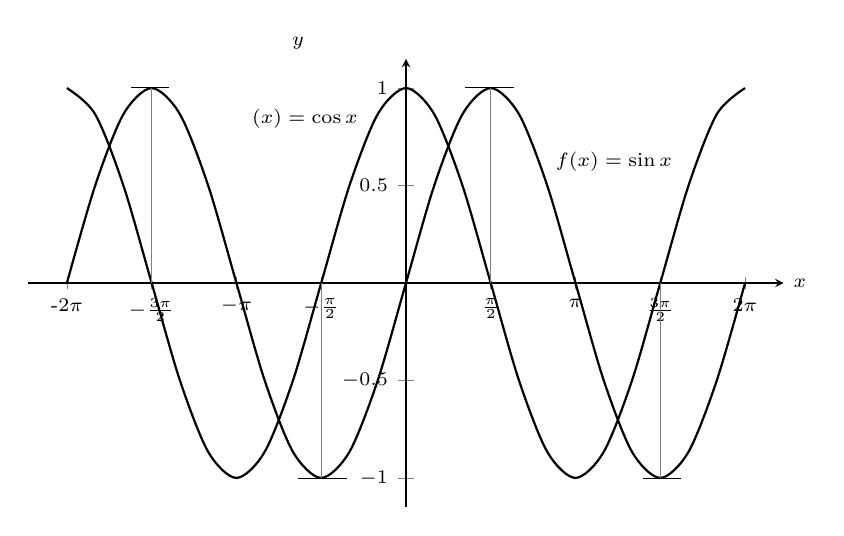
\begin{tikzpicture}
\begin{axis}[tick label style={font=\scriptsize}, axis y line=middle,axis x line=middle, ymin=-1.15, ymax=1.15,xmin=-7,xmax=7,name=myplot,  xtick={-6.28318, -4.7123889, -3.14159, -1.5708, 1.5708, 3.14159, 4.7123889, 6.28318}, xticklabels={-$2\pi$, $-\frac{3\pi}{2}$,$-\pi$, $-\frac{\pi}{2}$, $\frac{\pi}{2}$,$\pi$, $\frac{3\pi}{2}$, $2\pi$}, xscale=1.4]
\addplot [{\colorone}, smooth, domain=-6.28318:6.28318,thick] {sin(deg(x))} 
         node [pos=.7, above right] {\scriptsize $f(x)=\sin{x}$};
\addplot [{\colortwo},smooth, domain=-6.28318:6.28318,thick] {cos(deg(x))}
         node [pos=.45, above left] {\scriptsize $\fp(x)=\cos{x}$};
\draw[\colortwo] (axis cs:-5.1,1.005)--(axis cs:-4.4,1.005);
\draw[\colortwo] (axis cs:-2,-1.005)--(axis cs:-1.1,-1.005);
\draw[\colortwo] (axis cs:5.1,-1.005)--(axis cs:4.4,-1.005);
\draw[\colortwo] (axis cs:2,1.005)--(axis cs:1.1,1.005);  
\draw[gray] (axis cs:-4.7123889,0)--(axis cs:-4.7123889,1);
\draw[gray] (axis cs:-1.5708,0)--(axis cs:-1.5708,-1);
\draw[gray] (axis cs:1.5708,0)--(axis cs:1.5708,1);
\draw[gray] (axis cs:4.7123889,0)--(axis cs:4.7123889,-1);
\end{axis}
\node [right] at (myplot.right of origin) {\scriptsize $x$};
\node [above] at (myplot.above origin) {\scriptsize $y$};
\end{tikzpicture}
\caption{The function $f(x)=\sin x$ and its derivative $\fp(x)=\cos x$.}
\label{fig:sin_and_dsin}
\end{lxfigure}

Initially, this might be somewhat surprising; the result of a tedious limit process and the sine function is a nice function. Then again, perhaps this is not entirely surprising. The sine function is periodic --- it repeats itself on regular intervals. Therefore its rate of change also repeats itself on the same regular intervals. In fact, if we think about $\fp(x)$ as the slope of the tangent to the sine curve we notice the following
\begin{itemize}
\item when the slope of tangent lines is 0 then $\fp(x)=\cos x$ crosses the $x-$axis;
\item when the slopes of the tangent lines are positive then $\fp$ lies above the $x-$axis; and 
\item when the slopes of the tangent lines are negative then $\fp$ lies below the $x-$axis.
\end{itemize}

We should have known the derivative would be periodic; we now know exactly which periodic function it is.

Thinking back to \autoref{ex_der_num_approx}, we can find the slope of the tangent line to $f(x)=\sin x$ at $x=0$ using our derivative. We approximated the slope as $0.9983$; we now know the slope is \textit{exactly} $\cos 0 =1$.

\clearpage

\example{ex_not_diff}{Finding the derivative of a piecewise defined function}{Find the derivative of the absolute value function,
\[f(x) = \abs{x} = \begin{cases}-x & x<0 \\ x & x\geq 0\end{cases}.\]
See \autoref{fig:absolutevalue}.}
{We need to evaluate $\ds \lim_{h\to0}\frac{f(x+h)-f(x)}{h}.$ As $f$ is piecewise-defined, we need to consider separately the limits when $x<0$ and when $x>0$. \\

\mfigure{0in}{The absolute value function, $f(x) = \abs{x}$. Notice how the slope of the lines (and hence the tangent lines) abruptly changes at $x=0$.}{fig:absolutevalue}{figures/figabsolutevalue}

When $x<0$:
	\begin{align*}
	\frac{d}{dx}\big(-x\big)
	&= \lim_{h\to 0}\frac{-(x+h) - (-x)}{h} \\
	&=	\lim_{h\to 0}\frac{-h}{h}\\
	&=	\lim_{h\to 0}-1 \\
	&=	-1.
	\end{align*}
When $x>0$, a similar computation shows that $\ds \frac{d}{dx}\big(x\big) = 1$. \\

We need to also find the derivative at $x=0$. By the definition of the derivative at a point, we have $$\fp(0) = \lim_{h\to0}\frac{f(0+h)-f(0)}{h}.$$ Since $x=0$ is the point where our function's definition switches from one piece to the other, we need to consider left and right-hand limits. Consider the following, where we compute the left and right hand limits side by side.\\
\begin{minipage}[b]{.49\linewidth}
\begin{align*}
\lim_{h\to0^-}\frac{f(0+h)-f(0)}{h} &= \\
\lim_{h\to0^-}\frac{-h-0}{h} &= \\
\lim_{h\to0^-}-1 & =-1
\end{align*}
\end{minipage}\rule{.5pt}{70pt}%
\begin{minipage}[b]{.49\linewidth}
\begin{align*}
\lim_{h\to0^+}\frac{f(0+h)-f(0)}{h} &= \\
\lim_{h\to0^+}\frac{h-0}{h} &= \\
\lim_{h\to0^+}1 & =1
\end{align*}
\end{minipage}
%		
%		$$\begin{array}{ccccc}
%		\displaystyle \lim_{h\to0}\frac{f(0+h)-f(0)}{h} & = & \displaystyle\lim_{h\to0^-}\frac{f(0+h)-f(0)}{h} &=&\displaystyle\lim_{h\to0^+}\frac{f(0+h)-f(0)}{h}\\
%	\rule{0pt}{20pt}	&= & \displaystyle\lim_{h\to0^-}\frac{-h-0}{h} &=&\displaystyle\lim_{h\to0^+}\frac{h-0}{h}\\
%	\rule{0pt}{15pt}	&= & \displaystyle\lim_{h\to0^-}-1 &=&\displaystyle\lim_{h\to0^+}1\\
%	\rule{0pt}{12pt}	&= & -1 &=& 1\\
%		\end{array}$$
%		
\mfigure{-1in}{A graph of the derivative of $f(x) = \abs{x}$.}{fig:absolutevalueprime}{figures/figabsolutevalueprime}

\noindent
The last lines of each column tell the story: the left and right hand limits are not equal. Therefore the limit does not exist at 0, and $f$ is not differentiable at 0; see \autoref{fig:absolutevalueprime}.
So we have $$\fp(x) = \begin{cases} -1 & x<0 \\ 1 & x>0\end{cases}.$$ 
At $x=0$, $\fp(x)$ does not exist; there is a jump discontinuity at 0. So $f(x) = \abs{x}$ is differentiable everywhere except at 0.}

The point of non-differentiability came where the piecewise defined function switched from one piece to the other. Our next example shows that this does not always cause trouble.\bigskip

\example{ex_diff_piecewise}{Finding the derivative of a piecewise defined function}{Find the derivative of $f(x)$, where $\ds f(x) = \begin{cases}\sin x & x\leq \pi/2 \\ 1 & x>\pi/2 \end{cases}.$ See \autoref{fig:piecewisesinx1}.}
{Using \autoref{ex_deriv_sinx}, we know that when $x<\pi/2$, $\fp(x) = \cos x$. It is easy to verify that when $x>\pi/2$, $\fp(x) = 0$; consider:
\mfigure{0in}{A graph of $f(x)$ as defined in \autoref{ex_diff_piecewise}.}{fig:piecewisesinx1}{figures/figpiecewisesinx1}
\[
 \lim_{h\to0}\frac{f(x+h) - f(x)}{h}
 = \lim_{h\to0}\frac{1-1}{h} = \lim_{h\to0}0 =0.
\]

So far we have $$\fp(x) = \begin{cases}\cos x & x<\pi/2\\ 0 & x>\pi/2\end{cases}.$$ We still need to find $\fp(\pi/2)$. Notice at $x=\pi/2$ that both pieces of $\fp$ are 0, meaning we can state that $\fp(\pi/2)=0$. 

Being more rigorous, we can again evaluate the difference quotient limit at $x=\pi/2$, utilizing again left and right--hand limits:\\

\small
\noindent\begin{minipage}{.59\linewidth}
\begin{align*}
\lim_{h\to0^-}\frac{f(\pi/2+h)-f(\pi/2)}{h} &=\\
\lim_{h\to0^-}\frac{\sin(\pi/2+h)-\sin(\pi/2)}{h}&=\\
\lim_{h\to0^-}{ \frac{\sin(\frac{\pi}{2})\cos(h)+\sin(h)\cos(\frac{\pi}{2})-\sin(\frac{\pi}{2})}{h}}&=\\
\lim_{h\to0^-}\frac{1\cdot\cos(h)+\sin(h)\cdot 0-1}{h} &=\\
0
\end{align*}
\end{minipage}
\begin{minipage}{1pt}
 \rule{.5pt}{100pt}
\end{minipage}
\begin{minipage}{.39\linewidth}
\begin{align*}
\lim_{h\to0^+}\frac{f(\pi/2+h)-f(\pi/2)}{h} &=\\
\lim_{h\to0^+}\frac{1-1}{h}&=\\
\lim_{h\to0^+}\frac{0}{h}&=\\
0&\\
\phantom{0}\\
\phantom{0}
\end{align*}
\end{minipage}
\normalsize

%$\ds \lim_{h\to0}\frac{f(\pi/2+h)-f(\pi/2)}{h}=$
%\begin{align*}
% \lim_{h\to0^-}\frac{f(\pi/2+h)-f(\pi/2)}{h}
% &=\lim_{h\to0^+}\frac{f(\pi/2+h)-f(\pi/2)}{h}\\
% \lim_{h\to0^-}\frac{\sin(\pi/2+h)-\sin(\pi/2)}{h} &=\lim_{h\to0^+}\frac{1-1}{h}\\
% \lim_{h\to0^-}{ \frac{\sin(\pi/2)\cos(h)+\sin(h)\cos(\pi/2)-\sin(\pi/2)}{h}}
% &=\lim_{h\to0^+}\frac{0}{h}\\
% \lim_{h\to0^-}\frac{1\cdot\cos(h)+\sin(h)\cdot 0-1}{h} &=\lim_{h\to0^+}0\\
% 0 &=0\\
%\end{align*}
\mfigure{0in}{A graph of $\fp(x)$ in \autoref{ex_diff_piecewise}.}{fig:piecewisecosx1}{figures/figpiecewisecosx1}
Since both the left and right hand limits are 0 at $x=\pi/2$, the limit exists and $\fp(\pi/2)$ exists (and is 0). Therefore we can fully write $\fp$ as $$\fp(x) = \begin{cases}\cos x & x\leq\pi/2\\ 0 & x>\pi/2\end{cases}.$$ See \autoref{fig:piecewisecosx1} for a graph of this function.}

Recall we pseudo-defined a continuous function as one in which we could sketch its graph without lifting our pencil. We can give a pseudo--definition for differentiability as well: it is a continuous function that does not have any ``sharp corners.'' One such sharp corner is shown in \autoref{fig:absolutevalue}. Even though the function $f$ in \autoref{ex_diff_piecewise} is piecewise--defined, the transition is ``smooth'' hence it is differentiable. Note how in the graph of $f$ in \autoref{fig:piecewisesinx1} it is difficult to tell when $f$ switches from one piece to the other; there is no ``corner.''

\ifthenelse{\boolean{latexml}}{%
 To better understand the definition of a derivative, experiment with the Geogebra app at \url{http://mathinsight.org/applet/secant_line_slope}.%
% todo Tim : iframe ?
}{%
 \exvideo{%
  \begin{minipage}[t]{2cm}%
   \vspace{-.5\baselineskip}\qrcode{http://mathinsight.org/applet/secant_line_slope}%
  \end{minipage}
  \quad
  \begin{minipage}[t]{.74\linewidth}%
   To better understand the definition of a derivative, experiment with the Geogebra app at \\
   \url{http://mathinsight.org/applet/secant_line_slope}.%
  \end{minipage}%
 }%
}

This section defined the derivative; in some sense, it answers the question of ``What \textit{is} the derivative?'' The next section addresses the question ``What does the derivative \textit{mean}?''


\printexercises{exercises/02_01_exercises}

\section{Interpretations of the Derivative}\label{sec:interp_deriv}

The previous section defined the derivative of a function and gave examples of how to compute it using its definition (i.e., using limits). The section also started with a brief motivation for this definition, that is, finding the instantaneous velocity of a falling object given its position function. The next section will give us more accessible tools for computing the derivative, tools that are easier to use than repeated use of limits.

This section falls in between the ``What is the definition of the derivative?'' and ``How do I compute the derivative?'' sections. Here we are concerned with ``What does the derivative mean?'', or perhaps, when read with the right emphasis, ``What \textit{is} the derivative?'' We offer two interconnected interpretations of the derivative, hopefully explaining why we care about it and why it is worthy of study.\index{derivative!interpretation}

\subsection{Interpretation of the Derivative \#1: Instantaneous Rate of Change}

The previous section started with an example of using the position of an object (in this case, a falling amusement-park rider) to find the object's velocity. This type of example is often used when introducing the derivative because we tend to readily recognize that velocity is the \textit{instantaneous rate of change of position.} In general, if $f$ is a function of $x$, then $\fp(x)$ measures the instantaneous rate of change of $f$ with respect to $x$. Put another way, the derivative answers ``When $x$ changes, at what rate does $f$ change?'' Thinking back to the amusement-park ride, we asked ``When time changed, at what rate did the height change?'' and found the answer to be ``By $-64$ feet per second.'' 

Now imagine driving a car and looking at the speedometer, which reads ``60 mph.'' Five minutes later, you wonder how far you have traveled. Certainly, lots of things could have happened in those 5 minutes; you could have intentionally sped up significantly, you might have come to a complete stop, you might have slowed to 20 mph as you passed through construction.  But suppose that you know, as the driver, none of these things happened. You know you maintained a fairly consistent speed over those 5 minutes. What is a good approximation of the distance traveled?

One could argue the \textit{only} good approximation, given the information provided, would be based on ``distance = rate $\times$ time.'' In this case, we assume a constant rate of 60 mph with a time of $5/60$ hours. Hence we would approximate the distance traveled as 5 miles.\bigskip


Referring back to the falling amusement-park ride, knowing that at $t=2$ the velocity was $-64$ ft/s, we could reasonably assume that 1 second later the riders' height would have dropped by about 64 feet. Knowing that the riders were \textit{accelerating} as they fell would inform us that this is an \textit{under-approximation}. If all we knew was that $f(2) = 86$ and $\fp(2) = -64$, we'd know that we'd have to stop the riders quickly otherwise they would hit the ground!

\subsubsection{Units of the Derivative}

It is useful to recognize the \textit{units} of the derivative function. If $y$ is a function of $x$, i.e., $y=f(x)$ for some function $f$, and $y$ is measured in feet and $x$ in seconds, then the units of $y' = \fp$ are ``feet per second,'' commonly written as ``ft/s.'' In general, if $y$ is measured in units $P$ and $x$ is measured in units $Q$, then $y'$ will be measured in units ``$P$ per $Q$'', or ``$P/Q$.'' Here we see the fraction-like behavior of the derivative in the notation:
	\begin{center}
	the units of $\quad\ds \frac{dy}{dx}$\quad are \quad$\ds \frac{\text{units of $y$}}{\text{units of $x$}}$.
	\end{center}

\example*{ex_der_meaning1}{The meaning of the derivative: World Population}
{Let $P(t)$ represent the world population $t$ minutes after 12:00 a.m., January 1, 2012. It is fairly accurate to say that $P(0) = 7,028,734,178$ (\texttt{www.prb.org}). It is also fairly accurate to state that $P\primeskip'(0) = 156$; that is, at midnight on January 1, 2012, the population of the world was growing by about 156 \textit{people per minute} (note the units). Twenty days later (or, 28,800 minutes later) we could reasonably assume the population grew by about $(28,800)(156) = 4,492,800$ people.}

\example{ex_der_meaning2}{The meaning of the derivative: Manufacturing}{The term \textit{widget} is an economic term for a generic unit of manufacturing output. Suppose a company produces widgets and knows that the market supports a price of \$10 per widget. Let $P(n)$ give the profit, in dollars, earned by manufacturing and selling $n$ widgets. The company likely cannot make a (positive) profit making just one widget; the start-up costs will likely exceed \$10. Mathematically, we would write this as $P(1) < 0$.

What do $P(1000) = 500$ and $P\primeskip'(1000)=0.25$ mean? Approximate $P(1100)$.}
{The equation $P(1000)=500$ means that selling 1,000 widgets returns a profit of \$500. We interpret $P\primeskip'(1000) = 0.25$ as meaning that when producing 1000 widgets, the profit is increasing at rate of \$0.25 per widget (the units are ``dollars per widget.'') Since we have no other information to use, our best approximation for $P(1100)$ is:
\[P(1100)\approx P(1000)+P\primeskip'(1000)\times100=\$500+100\cdot0.25=\$525.\]
We approximate that selling 1,100 widgets returns a profit of \$525.}

The previous examples made use of an important approximation tool that we first used in our previous ``driving a car at 60 mph'' example at the beginning of this section. Five minutes after looking at the speedometer, our best approximation for distance traveled assumed the rate of change was constant. In Examples \ref{ex_der_meaning1} and \ref{ex_der_meaning2} we made similar approximations. We were given rate of change information which we used to approximate total change. Notationally, we would say that 
\[f(c+h) \approx f(c) + \fp(c)\cdot h.\]
This approximation is best when $h$ is ``small.'' ``Small'' is a relative term; when dealing with the world population, $h=$ 22 days = 28,800 minutes is small in comparison to years. When manufacturing widgets, 100 widgets is small when one plans to manufacture thousands.

% If $C(t)$ measures the number of customers in a store at time $t$, where $t$ is measured in hours since opening, then $C'(t)$ measures the rate at which the number of customers is increasing per hour. Suppose 2 hours after opening there are 50 customers in a store; this means $C(2) = 50$. Suppose further that $C'(2) = 20$. That means that 2 hours after opening, customers are coming into the store at a rate of 20 per hour. One could then reasonably assume that 3 hours after opening the store would have about 70 customers in it. (And 2.5 hours after opening the store would have about 60 customers in it.) If one were to plot the number of people in the 

\subsection{The Derivative and Motion}

One of the most fundamental applications of the derivative is the study of motion. Let $s(t)$ be a position function, where $t$ is time and $s(t)$ is  distance. For instance, $s$ could measure the height of a projectile or the distance an object has traveled. 

Let's let $s(t)$ measure the distance traveled, in feet, of an object after $t$ seconds of travel. Then $s\primeskip'(t)$ has units ``feet per second,'' and $s\primeskip'(t)$ measures the \textit{instantaneous rate of distance change} --- it measures \textbf{velocity}.\index{velocity} 

Now consider $v(t)$, a velocity function. That is, at time $t$, $v(t)$ gives the velocity of an object. The derivative of $v$, $v\primeskip'(t)$, gives the \textit{instantaneous rate of velocity change} ---
\textbf{acceleration}. (We often think of acceleration in terms of cars: a car may ``go from 0 to 60 in 4.8 seconds.'' This is an \textit{average} acceleration, a measurement of how quickly the velocity changed.) If velocity is measured in feet per second, and time is measured in seconds, then the units of acceleration (i.e., the units of $v\primeskip'(t)$) are ``feet per second per second,'' or $($ft/s$)$/s. We often shorten this to ``feet per second squared,'' or ft/s$^2$, but this tends to obscure the meaning of the units.\index{acceleration}

Perhaps the most well known acceleration is that of gravity. In this text, we use $g=32$ft/s$^2$ or $g=9.8$m/s$^2$. What do these numbers mean?

A constant acceleration of 32$($ft/s$)$/s means that the velocity changes by 32ft/s each second. For instance, let $v(t)$ measures the velocity of a ball thrown straight up into the air, where $v$ has units ft/s and $t$ is measured in seconds. The ball will have a positive velocity while traveling upwards and a negative velocity while falling down. The acceleration is thus $-32$ft/s$^2$. If $v(1) = 20$ft/s, then when $t=2$, the velocity will have decreased by 32ft/s; that is, $v(2) = -12$ft/s. We can continue: $v(3) = -44$ft/s, and we can also figure that $v(0) = 52$ft/s.

These ideas are so important we write them out as a Key Idea.

\begin{keyidea}[The Derivative and Motion]\label{idea:motion}
~\\[-2\baselineskip]\begin{enumerate}
	\item Let $s(t)$ be the position function of an object. Then $s\primeskip'(t)$ is the velocity function of the object.
	\item	Let $v(t)$ be the velocity function of an object. Then $v\primeskip'(t)$ is the acceleration function of the object.
\end{enumerate}%
\index{derivative!motion}\index{derivative!velocity}\index{derivative!acceleration}
\end{keyidea}

We now consider the second interpretation of the derivative given in this section. This interpretation is not independent from the first by any means; many of the same concepts will be stressed, just from a slightly different perspective.

\subsection{Interpretation of the Derivative \#2: The Slope of the Tangent Line}

Given a function $y=f(x)$, the difference quotient $\ds \frac{f(c+h)-f(c)}{h}$ gives a change in $y$ values divided by a change in $x$ values; i.e., it is a measure of the ``rise over run,'' or ``slope,'' of the line that goes through two points on the graph of $f$: $\big(c, f(c)\big)$ and $\big(c+h,f(c+h)\big)$. As $h$ shrinks to 0, these two points come close together; in the limit we find $\fp(c)$, the slope of a special line called the tangent line. % that intersects $f$ only once near $x=c$.

Lines have a constant rate of change, their slope. Nonlinear functions do not have a constant rate of change, but we can measure their \textit{instantaneous rate of change} at a given $x$ value $c$ by computing $\fp(c)$. We can get an idea of how $f$ is behaving by looking at the slopes of its tangent lines. We explore this idea in the following example.

\youtubeVideo{CpDfay5NeCg}{Interpreting slope of a curve exercise}

\mtable{A graph of $f(x)=x^2$ and tangent lines.}{fig:xsquared}{\begin{tikzpicture}
\begin{axis}[width=1.16\marginparwidth,tick label style={font=\scriptsize},
ytick={0,4,8,12,16},minor x tick num=0,minor y tick num=3,axis y line=middle,
axis x line=middle,ymin=-.4,ymax=17,xmin=-.1,xmax=4.1,name=myplot,grid=major]
\addplot [draw={\colorone},smooth,thick,domain=-.1:4.1] {x*x};
\addplot [draw={\colortwo},domain=0:4]{2*(x-1)+1};
\addplot [draw={\colortwo},domain=1.5:4]{6*(x-3)+9};
\end{axis}
\node [right] at (myplot.right of origin) {\scriptsize $x$};
\node [above] at (myplot.above origin) {\scriptsize $y$};
\end{tikzpicture}}

\example{ex_der_meaning3}{Understanding the derivative: the rate of change}{Consider $f(x) = x^2$ as shown in \autoref{fig:xsquared} with tangent lines at $x=1$ and $x=3$. It is clear that at $x=3$ the function is growing faster than at $x=1$, as it is steeper at $x=3$. How much faster is it growing?}
{We can answer this directly after the following section, where we learn to quickly compute derivatives. For now, we will answer graphically, by considering the slopes of the respective tangent lines.

With practice, one can fairly effectively sketch tangent lines to a curve at a particular point. In \autoref{fig:xsquared}, we have sketched the tangent lines to $f$ at $x=1$ and $x=3$, along with a grid to help us measure the slopes of these lines. At $x=1$, the slope is 2; at $x=3$, the slope is 6. Thus we can say not only is $f$ growing faster at $x=3$ than at $x=1$, it is growing \textit{three times as fast}.}

\mtable{Graphs of $f$ and $\fp$ in \autoref{ex_der_meaning4}, along with tangent lines.}{fig:fwithderiv}{\begin{tikzpicture}
\begin{axis}[width=1.16\marginparwidth,tick label style={font=\scriptsize},
minor x tick num=1,minor y tick num=4,axis y line=middle,axis x line=middle,
ymin=-8.9,ymax=5.9,xmin=-.1,xmax=3.49,name=myplot]
\addplot [draw={\colorone},smooth,thick,domain=0:3.5] {-x^3+7*x^2-12*x+4};
\addplot [draw={\colortwo},smooth,thick,domain=0:3.5] {-12+14*x-3*x^2};
\addplot [domain=0:2,thick] {-1*(x-1)-2};
\addplot [domain=1:3,thick] {4*(x-2)};
\addplot [domain=2:4,thick] {3*(x-3)+4};
\filldraw [draw={\colortwo}] (axis cs:1,-1) circle (1pt);
\filldraw [draw={\colortwo}] (axis cs:2,4) circle (1pt);
\filldraw [draw={\colortwo}] (axis cs:3,3) circle (1pt);
\draw (axis cs:3.25,5.5) node {\scriptsize $f(x)$};
\draw (axis cs:1.25,3) node {\scriptsize $f\,'(x)$};
\end{axis}
\node [right] at (myplot.right of origin) {\scriptsize $x$};
\node [above] at (myplot.above origin) {\scriptsize $y$};
\end{tikzpicture}}

\example{ex_der_meaning4}{Understanding the graph of the derivative}{Consider the graph of $f(x)$ and its derivative, $\fp(x)$, in \autoref{fig:fwithderiv}.
%f[x_] := InterpolatingPolynomial[{-1, 0, 2}, x]*4,MAKE BIGGER, PLOT THIS WITH F' NO INTEGRATE,IDIOT
Use these graphs to find the slopes of the tangent lines to the graph of $f$ at $x=1$, $x=2$, and $x=3$.%
}%Because of interp poly, we have \fp = -1, 0, 2 respectively
{To find the appropriate slopes of tangent lines to the graph of $f$, we need to look at the corresponding values of $\fp$.

The slope of the tangent line to $f$ at $x=1$ is $\fp(1)$; this looks to be about $-1$.

The slope of the tangent line to $f$ at $x=2$ is $\fp(2)$; this looks to be about $4$. 

The slope of the tangent line to $f$ at $x=3$ is $\fp(3)$; this looks to be about $3$. 

Using these slopes, the tangent lines to $f$ are sketched in \autoref{fig:fwithderiv} as well. Included on the graph of $\fp$ in this figure are filled circles where $x=1$, $x=2$ and $x=3$ to help better visualize the $y$ value of $\fp$ at those points.}

% todo maybe change example 2.2.5 so that f'(3)!=3
\example{ex_der_meaning5}{Approximation with the derivative}{Consider again the graph of $f(x)$ and its derivative $\fp(x)$ in \autoref{ex_der_meaning4}.
%
\mtable{Zooming in on $f$ and its tangent line at $x=3$ for the function given in Examples \ref{ex_der_meaning4} and \ref{ex_der_meaning5}.}{fig:fwithderivzoom3}{\begin{tikzpicture}
\begin{axis}[width=1.16\marginparwidth,tick label style={font=\scriptsize},
minor x tick num=1,minor y tick num=4,axis y line=middle,
axis x line=middle,ymin=1.9,ymax=4.9,xmin=2.7,xmax=3.3,name=myplot]
\addplot [draw={\colorone},smooth,thick,domain=2.7:3.3] {-x^3+7*x^2-12*x+4};
\addplot [domain=2.7:3.3,thick] {3*(x-3)+4};
\end{axis}
\node [right] at (myplot.right of origin) {\scriptsize $x$};
\node [above] at (myplot.above origin) {\scriptsize $y$};
\end{tikzpicture}}
%
Use the tangent line to $f$ at $x=3$ to approximate the value of $f(3.1)$.}
{\autoref{fig:fwithderivzoom3} shows the graph of $f$ along with its tangent line, zoomed in at $x=3$. Notice that near $x=3$, the tangent line makes an excellent approximation of $f$. Since lines are easy to deal with, often it works well to approximate a function with its tangent line. (This is especially true when you don't actually know much about the function at hand, as we don't in this example.)

While the tangent line to $f$ was drawn in \autoref{ex_der_meaning4}, it was not explicitly computed. Recall that the tangent line to $f$ at $x=c$ is $y = \fp(c)(x-c)+f(c)$. While $f$ is not explicitly given, by the graph it looks like $f(3) = 4$. Recalling that $\fp(3) = 3$, we can compute the tangent line to be approximately $y = 3(x-3)+4.$ It is often useful to leave the tangent line in point-slope form.

To use the tangent line to approximate $f(3.1)$, we simply evaluate $y$ at $3.1$ instead of $f$.
\[f(3.1) \approx y(3.1) = 3(3.1-3)+4 = .1*3+4 = 4.3.\]
We approximate $f(3.1) \approx 4.3.$}

To demonstrate the accuracy of the tangent line approximation, we now state that in \autoref{ex_der_meaning5}, $f(x) = -x^3+7x^2-12x+4$. We can evaluate $f(3.1) = 4.279$. Had we known $f$ all along, certainly we could have just made this computation. In reality, we often only know two things:
\begin{enumerate}
	\item	What $f(c)$ is, for some value of $c$, and
	\item	what $\fp(c)$ is.
\end{enumerate}
	
For instance, we can easily observe the location of an object and its instantaneous velocity at a particular point in time. We do not have a ``function $f$\ '' for the location, just an observation. This is enough to create an approximating function for $f$.

This last example has a direct connection to our approximation method explained above after \autoref{ex_der_meaning2}. We stated there that
\[f(c+h) \approx f(c)+\fp(c)\cdot h.\]
If we know $f(c)$ and $\fp(c)$ for some value $x=c$, then computing the tangent line at $(c,f(c))$ is easy: $y(x) = \fp(c)(x-c)+f(c)$. In \autoref{ex_der_meaning5}, we used the tangent line to approximate a value of $f$. Let's use the tangent line at $x=c$ to approximate a value of $f$ near $x=c$; i.e., compute $y(c+h)$ to approximate $f(c+h)$, assuming again that $h$ is ``small.'' Note:
\[y(c+h) = \fp(c)\big((c+h)-c\big)+f(c) = \fp(c)\cdot h + f(c).\]
This is the exact same approximation method used above! Not only does it make intuitive sense, as explained above, it makes analytical sense, as this approximation method is simply using a tangent line to approximate a function's value.\bigskip\bigskip


The importance of understanding the derivative cannot be understated. When $f$ is a function of $x$, $\fp(x)$ measures the instantaneous rate of change of $f$ with respect to $x$ and gives the slope of the tangent line to $f$ at $x$.

\printexercises{exercises/02_02_exercises}

% todo find an interactive where you specify the function and overlay f and f'
\section{Basic Differentiation Rules}\label{sec:basic_diff_rules}

The derivative is a powerful tool but is admittedly awkward given its reliance on limits. Fortunately, one thing mathematicians are good at is \emph{abstraction.} For instance, instead of continually finding derivatives at a point, we abstracted and found the derivative function. 

Let's practice abstraction on linear functions, $y=mx+b$. What is $y\primeskip'$? Without limits, recognize that linear functions are characterized by being functions with a constant rate of change (the slope). The derivative, $y\primeskip'$, gives the instantaneous rate of change; with a linear function, this is constant, $m$. Thus $y\primeskip'=m$. 

Let's abstract once more. Let's find the derivative of the general quadratic function, $f(x) = ax^2+bx+c$. Using the definition of the derivative, we have:
\begin{align*}
	\fp(x)
	&=	\lim_{h\to 0}\frac{a(x+h)^2+b(x+h)+c-(ax^2+bx+c)}{h} \\
	&=	\lim_{h\to 0} \frac{ah^2+2ahx+bh}{h} \\
	&=	\lim_{h\to 0}(ah+2ax+b)\\
	&= 2ax+b.
\end{align*}
		
So if $y = 6x^2+11x-13$, we can immediately compute $y\primeskip' = 12x+11$.\bigskip

In this section (and in some sections to follow) we will learn some of what mathematicians have already discovered about the derivatives of certain functions and how derivatives interact with arithmetic operations. We start with a theorem.

\begin{anywhereenum}
\begin{theorem}[Derivatives of Common Functions]\label{thm:deriv_common}
\noindent\index{derivative!basic rules}\index{derivative!Constant Rule}\index{derivative!Power Rule}\index{Power Rule!differentiation}%
\tagpdfsetup{table/tagging=presentation}
\begin{tabular}{ll}
\item \textbf{Constant Rule:}	$\dfrac \dd{\dd x}\bigl( c\bigr) = 0$, &
\item \textbf{Power Rule:} $\dfrac \dd{\dd x}\left(x^n\right) = nx^{n-1}$,\\
\null\qquad where $c$ is a constant. &
\null\qquad where $n$ is any real number.\\
\item $\dfrac \dd{\dd x}(\sin x) = \cos x$ &
\item $\dfrac \dd{\dd x}(\cos x) = -\sin x$ \\[2ex]
\item $\dfrac \dd{\dd x}\left(e^x\right) = e^x$ &
\item $\dfrac \dd{\dd x}(\ln x) = \dfrac1x$
\end{tabular}
\end{theorem}
\end{anywhereenum}

This theorem starts by stating an intuitive fact: constant functions have a rate of change of zero, as they are \emph{constant}. Therefore their derivative is 0. The proof is left as an exercise.

The theorem then states some fairly amazing things.

In Part 2, the Power Rule states that the derivatives of functions of the form $y=x^n$ where $\mathbf{n}$ \textbf{is ANY real number} are very straightforward: multiply by the power, then subtract 1 from the power. This allows us to differentiate Power Functions, Root Functions, and functions with irrational exponents. The work we have done so far only allows us to prove the Power Rule when $n$ is a non-negative integer, which is presented here. We will provide proofs for other values of $n$ as we add the necessary tools to our knowledge of calculus.

\begin{proof}[Proof of Differentiation Power Rule when $n$ is a non-negative integer]
If $n=0$, then $f(x)=x^0=1$ (except when $x=0$, when the expression is indeterminate).  This means that
\[\fp(x)=\lim_{h\to0}\frac{1-1}h=\lim_{h\to0}\frac0h=0=0x^{0-1}\]
as claimed.  Now let $f(x)= x^n$, where $n \in \mathbb{Z}^+$. By the definition of derivative,
\begin{align*}
\fp(x)
&= \lim_{h\to 0} \dfrac{(x+h)^n - x^n}{h} \\
&= \lim_{h\to 0} \dfrac{(x+h)^n - x^n}{h} \qquad\text{\small use the Binomial Theorem to expand $(x+h)^n$} \\
&=\lim_{h\to 0} \dfrac{\binom{n}{0}x^n + \binom{n}{1} hx^{n-1} + \binom{n}{2} h^2x^{n-2}+ \dotsb +\binom{n}{n-1} h^{n-1}x + \binom {n}{n} h^n  -x^n}{h} \\
&= \lim_{h\to 0} \dfrac{\binom{n}{1} hx^{n-1} + \binom{n}{2} h^2x^{n-2}+ \dotsb +\binom{n}{n-1} h^{n-1}x + \binom{n}{n} h^n}{h} \\
&= \lim_{h\to 0} \dfrac{h\left[\binom{n}{1} x^{n-1} + \binom{n}{2} h x^{n-2}+ \dotsb +\binom{n}{n-1} h^{n-2}x + \binom {n}{n} h^{n-1}\right]}{h},\text{\small~divide $h$}\\
&= \lim_{h\to 0}\left[\dbinom{n}{1} x^{n-1} + \dbinom{n}{2} h x^{n-2}+ \dotsb +\dbinom{n}{n-1} h^{n-2}x + \dbinom {n}{n} h^{n-1}\right],\\
&=  n x^{n-1} \qquad\text{\small since } \dbinom{n}{1} = n \qedhere
\end{align*}
\end{proof}

We proved \autoref{thm:deriv_common} part 3 in \autoref{sec:derivative} and part 4 is left as an exercise.  In parts 5 and 6 we see something incredible about the functions $y=e^x$ and $y=\ln x$. We will use these rules freely, unfortunately their proofs will have to wait until we know a few more calculus techniques.
% it is its own derivative.

%One special case of the Power Rule is when $n=1$, i.e., when $f(x) = x$. What is $\fp(x)$? According to the Power Rule, \[\fp(x) = \frac{\dd}{\dd x}\bigl(x\bigr) = \frac{\dd}{\dd x}\bigl(x^1\bigr) = 1\cdot x^0 = 1.\] In words, we are asking ``At what rate does $f$ change with respect to $x$?'' Since $f$ \emph{is} $x$, we are asking ``At what rate does $x$ change with respect to $x$?'' The answer is: 1. They change at the same rate.\\

Let's practice using this theorem.

\begin{example}[Using \autoref{thm:deriv_common} to find, and use, derivatives]\label{ex_deriv_rule1}
Let $f(x)=x^3$. 
\begin{enumerate}
	\item	Find $\fp(x)$.
	\item	Find the equation of the line tangent to the graph of $f$ at $x=-1$. 
	\item	Use the tangent line to approximate $(-1.1)^3$.
	\item	Sketch $f$, $\fp$ and the found tangent line on the same axis.
\end{enumerate}
\solution
\begin{enumerate}
	\item	The Power Rule states that if $f(x) = x^3$, then $\fp(x) = 3x^2$. 
	\item	To find the equation of the line tangent to the graph of $f$ at $x=-1$, we need a point and the slope. The point is $(-1,f(-1)) = (-1, -1)$. The slope is $\fp(-1)= 3$. Thus the tangent line has equation $y = 3(x-(-1))+(-1) = 3x+2$. 

	\mtable{A graph of $f(x) = x^3$, along with its derivative $\fp(x) = 3x^2$ and its tangent line at $x=-1$.}{fig:xcubedwithderiv}{\pdftooltip{\begin{tikzpicture}
\begin{axis}[width=1.16\marginparwidth,tick label style={font=\scriptsize},minor x tick num=1,minor y tick num=1,axis y line=middle,axis x line=middle,ymin=-5.1,ymax=5.1,xmin=-2.1,xmax=2.1,name=myplot]
\addplot [draw={\colorone},smooth,thick,domain=-2:2] {x^3};
\addplot [draw={\colortwo},smooth,thick,domain=-2:2] {3*x^2};
\addplot [smooth,thick,domain=-2:1.2] {3*(x+1)-1};
\filldraw (axis cs:-1,-1) circle (1pt);
\filldraw (axis cs:-1,3) circle (1pt);
\end{axis}
\node [right] at (myplot.right of origin) {\scriptsize $x$};
\node [above] at (myplot.above origin) {\scriptsize $y$};
\end{tikzpicture}}{A curve that begins near (-1.5,-3.5), moves upward and flattens out to go through the origin, and then curves upward to finish near (1.5, 3.5).  A second curve is U shaped, going through the points (-1,3), the origin, and (1,3).  A line is tangent to the first curve at the point (-1,-1).  The slope of this line is 3, so that the second curve goes through the point (-1,3).}}
	\item	We can use the tangent line to approximate $(-1.1)^3$ as $-1.1$ is close to $-1$. We have
	\[(-1.1)^3 \approx (-1)^3+3(-1.1-(-1))=-1+3(-.1)= -1.3.\]
	We can easily find the actual answer; $(-1.1)^3 = -1.331$. 
	\item	See \autoref{fig:xcubedwithderiv}.
\end{enumerate}
\end{example}

\autoref{thm:deriv_common} gives useful information, but we will need much more. For instance, using the theorem, we can easily find the derivative of $y=x^3$, but it does not tell how to compute the derivative of $y=2x^3$, $y=x^3+\sin x$, nor $y=x^3\sin x$. The following theorem helps with the first two of these examples (the third is answered in the next section).

\begin{theorem}[Properties of the Derivative]\label{thm:deriv_prop}
Let $f$ and $g$ be differentiable on an open interval $I$ and let $c$ be a real number. Then:
\index{derivative!Sum/Difference Rule}\index{Sum/Difference Rule!of derivatives}
\index{derivative!Constant Multiple Rule}\index{Constant Multiple Rule!of derivatives}\begin{enumerate}
	\item	\textbf{Sum/Difference Rule:}\\
	\qquad$\ds \frac{\dd}{\dd x}\Bigl(f(x) \pm g(x)\Bigr) = \frac{\dd}{\dd x}\Bigl(f(x)\Bigr) \pm \frac{\dd}{\dd x}\Bigl(g(x)\Bigr)=\fp(x)\pm g\primeskip'(x)$
	\item	\textbf{Constant Multiple Rule:}\\
	\qquad$\ds \frac{\dd}{\dd x}\Bigl(c\cdot f(x)\Bigr) = c\cdot\frac{\dd}{\dd x}\Bigl(f(x)\Bigr) = c\cdot\fp(x)$.
\end{enumerate}
\end{theorem}

\begin{proof}[Proof of Sum Rule for Differentiation]
Let $f$ and $g$ be differentiable on an open interval $I$ and let $c$ be a real number,
\begin{align*}
\frac{\dd}{\dd x}( f(x) + g(x))
&= \lim_{h\to 0} \frac{[f(x+h)+g(x+h)] - [f(x)+g(x)]}{h} \\
&= \lim_{h\to 0} \frac{[f(x+h)-f(x)] + [g(x+h) - g(x)]}{h} \\
&= \lim_{h\to 0} \frac{[f(x+h)-f(x)]}{h} + \lim_{h\to 0}\frac {g(x+h) - g(x)}{h}\\
&= \fp(x) + g'(x)\qedhere
\end{align*}
\end{proof}

\youtubeVideo{3dJepii_rJ0}{Basic Derivative Examples}

\autoref{thm:deriv_prop} allows us to find the derivatives of a wide variety of functions. It can be used in conjunction with the Power Rule to find the derivatives of any polynomial. Recall in \autoref{ex_deriv1} that we found, using the limit definition, the derivative of $f(x) = 3x^2+5x-7$. We can now find its derivative without expressly using limits:
\begin{align*}
	\frac{\dd}{\dd x}\Bigl(3x^2+5x+7\Bigr)
	&= 3\frac{\dd}{\dd x}\Bigl(x^2\Bigr) + 5\frac{\dd}{\dd x}\Bigl(x\Bigr) + \frac{\dd}{\dd x}\Bigl(7\Bigr) \\
	&= 3\cdot 2x+5\cdot 1+ 0\\
	&= 6x+5.
\end{align*}

We were a bit pedantic here, showing every step. Normally we would do all the arithmetic and steps in our head and readily find $\ds \frac{\dd}{\dd x}\Bigl(3x^2+5x+7\Bigr) = 6x+5$.

\begin{example}[Using Theorems \ref{thm:deriv_common} and \ref{thm:deriv_prop} to find derivatives]\label{ex_der15}
Use Theorems \ref{thm:deriv_common} and \ref{thm:deriv_prop} to differentiate
\[\text{1. }g(x)=(x^2+1)^3\qquad\qquad\text{2. }f(x)=\ln\frac{\sqrt{x}}8\]
\solution
Given the differentiation rules we have thus far, our only option for finding $g'(x)$ is to first multiply $g(x)$ out and then apply the sum and power rules. We see that
\[g(x) = x^6 + 3x^4 + 3x^2 + 1\]
thus,\vspace{-.5\baselineskip}
\[g'(x) = 6x^5 + 12x^3 + 6x.\]

To differentiate $f(x)$ we will first need to use the Laws of Logarithms to expand $f$ as\vspace{-.5\baselineskip}
\begin{align*}
f(x)
&= \ln \frac{\sqrt x}{8}\\
&= \ln x^{\frac{1}{2}} - \ln 8 \\
&= \frac12\ln x - \ln 8 \\
\end{align*}
so that,\vspace{-.5\baselineskip}
\[\fp(x)=\frac12\cdot\frac1x-0=\frac12x.\]
\end{example}

\begin{example}[Using the tangent line to approximate a function value]\label{ex_der2}
Let $f(x) = \sin x + 2x+1$. Approximate $f(3)$ using an appropriate tangent line.
\solution
This problem is intentionally ambiguous; we are to \emph{approximate} using an \emph{appropriate} tangent line. How good of an approximation are we seeking? What does appropriate mean?

In the ``real world,'' people solving problems deal with these issues all time. One must make a judgment using whatever seems reasonable. In this example, the actual answer is $f(3) = \sin 3 + 7$, where the real problem spot is $\sin 3$. What is $\sin 3$?

Since $3$ is close to $\pi$, we can assume $\sin 3\approx \sin \pi = 0$. Thus one guess is $f(3) \approx 7$. Can we do better? Let's use a tangent line as instructed and examine the results; it seems best to find the tangent line at $x=\pi$. 

Using \autoref{thm:deriv_common} we find $\fp(x) = \cos x + 2$. The slope of the tangent line is thus $\fp(\pi) = \cos \pi + 2 =1$. Also, $f(\pi) = 2\pi+1 \approx 7.28$. So the tangent line to the graph of $f$ at $x=\pi$ is $y=1(x-\pi)+ 2\pi+1 =x+\pi+1 \approx x+4.14$. Evaluated at $x=3$, our tangent line gives $y=3+4.14 = 7.14$. Using the tangent line, our final approximation is that $f(3) \approx 7.14$.

Using a calculator, we get an answer accurate to 4 places after the decimal: $f(3) = 7.1411$. Our initial guess was $7$; our tangent line approximation was more accurate, at $7.14$.

The point is \emph{not} ``Here's a cool way to do some math without a calculator.'' Sure, that might be handy sometime, but your phone could probably give you the answer. Rather, the point is to say that tangent lines are a good way of approximating, and many scientists, engineers and mathematicians often face problems too hard to solve directly. So they approximate.
\end{example}

\subsection{Higher Order Derivatives}

The derivative of a function $f$ is itself a function, therefore we can take its derivative. The following definition gives a name to this concept and introduces its notation.

\begin{definition}[Higher Order Derivatives]\label{def:Higher_Deriv}
Let $y=f(x)$ be a differentiable function on $I$. \index{derivative!higher order}\index{derivative!notation}
	\begin{enumerate}
		\item	The \emph{second derivative} of $f$ is: 
			\[ \fp'(x) = \frac{\dd}{\dd x}\Bigl(\fp(x)\Bigr) = \frac{\dd}{\dd x}\left(\frac{\dd y}{\dd x}\right) = \frac{\dd^2y}{\dd x^2}=y\primeskip''.\]
		\item	The \emph{third derivative} of $f$ is: 
			\[ \fp''(x) = \frac{\dd}{\dd x}\Bigl(\fp'(x)\Bigr) = \frac{\dd}{\dd x}\left(\frac{\dd^2y}{\dd x^2}\right) = \frac{\dd^3y}{\dd x^3}=y\primeskip'''.\]
		\item	The \emph{n\textsuperscript{th} derivative} of $f$ is:
			\[ f\,^{(n)}(x) = \frac{\dd}{\dd x}\left(f\,^{(n-1)}(x)\right) = \frac{\dd}{\dd x}\left(\frac{\dd^{n-1}y}{\dd x^{n-1}}\right) = \frac{\dd^ny}{\dd x^n}=y^{(n)}.\]
	\end{enumerate}
\end{definition}

\mnote[-1in]{\textbf{Note:} \autoref{def:Higher_Deriv} comes with the caveat ``Where the corresponding limits exist.'' With $f$ differentiable on $I$, it is possible that $\fp$ is \emph{not} differentiable on all of $I$, and so on.}

In general, when finding the fourth derivative and on, we resort to the $f\,^{(4)}(x)$ notation, not $\fp'''(x)$; after a while, too many ticks is too confusing.\bigskip

Let's practice using this new concept.

\begin{example}[Finding higher order derivatives]\label{ex_high_order}
Find the first four derivatives of the following functions:
\[1.\ f(x) = 4x^2\qquad 2.\ f(x) = \sin x\qquad 3.\ f(x) = 5e^x\]
\solution
\begin{enumerate}
	\item	Using the Power and Constant Multiple Rules, we have: $\fp(x) = 8x$. Continuing on, we have 
	\[\fpp(x) = \frac{\dd}{\dd x}\bigl(8x\bigr) = 8;\qquad \fp''(x) = 0;\qquad f\,^{(4)}(x) = 0.\]
Notice how all successive derivatives will also be 0.
	\item	We employ \autoref{thm:deriv_common} repeatedly.
	\[\fp(x) = \cos x;\quad \fp'(x) = -\sin x;\quad \fp''(x) = -\cos x;\quad f\,^{(4)}(x) = \sin x.\]
	Note how we have come right back to $f(x)$ again. (Can you quickly figure what $f\,^{(23)}(x)$ is?)
	\item	Employing \autoref{thm:deriv_common} and the Constant Multiple Rule, we can see that
	\[\fp(x) = \fp'(x) = \fp''(x) = f\,^{(4)}(x) = 5e^x.\]
	\end{enumerate}
\end{example}

\subsection{Interpreting Higher Order Derivatives}

What do higher order derivatives \emph{mean}? What is the practical interpretation? \index{derivative!higher order!interpretation}

Our first answer is a bit wordy, but is technically correct and beneficial to understand. That is,
	\begin{quote}
	The second derivative of a function $f$ is the rate of change of the rate of change of $f$.
	\end{quote}

One way to grasp this concept is to let $f$ describe a position function. Then, as stated in \autoref{idea:motion}, $\fp$ describes the rate of position change: velocity. We now consider $\fp'$, which describes the rate of velocity change. Sports car enthusiasts talk of how fast a car can go from 0 to 60 mph; they are bragging about the \emph{acceleration} of the car.

We started this chapter with amusement-park riders free-falling with position function $f(t) = -16t^2+150$. It is easy to compute $\fp(t)=-32t$ ft/s and $\fp'(t) = -32$ (ft/s)/s. We may recognize this latter constant; it is the acceleration due to gravity. In keeping with the unit notation introduced in the previous section, we say the units are ``feet per second per second.'' This is usually shortened to ``feet per second squared,'' written as ``ft/s$^2$.''

It can be difficult to consider the meaning of the third, and higher order, derivatives. The third derivative is ``the rate of change of the rate of change of the rate of change of $f$.'' That is essentially meaningless to the uninitiated. In the context of our position/velocity/acceleration example, the third derivative is the ``rate of change of acceleration,'' commonly referred to as ``jerk.'' 

Make no mistake: higher order derivatives have great importance even if their practical interpretations are hard (or ``impossible'') to understand. The mathematical topic of \emph{series} makes extensive use of higher order derivatives.

\printexercises{exercises/02-03-exercises}

% todo Find an interactive where you specify f and see f, f', and f''

\section{The Product and Quotient Rules}\label{sec:prod_quot_rules}

The previous section showed that, in some ways, derivatives behave nicely. The Constant Multiple and Sum/Difference Rules established that the derivative of $f(x) = 5x^2+\sin x $ was not complicated. We neglected computing the derivative of things like $g(x) = 5x^2\sin x$ and $h(x) = \frac{5x^2}{\sin x}$ on purpose; their derivatives are \emph{not} as straightforward. (If you had to guess what their respective derivatives are, you would probably guess wrong.) For these, we need the Product and Quotient Rules, respectively, which are defined in this section. 

We begin with the Product Rule.

\begin{theorem}[Product Rule]\label{thm:ProductRule}
Let $f$ and $g$ be differentiable functions on an open interval $I$.\index{Product Rule!differentiation}\index{derivative!Product Rule} Then $f\cdot g$ is a differentiable function on $I$, and
\[\frac{\dd}{\dd x}\Bigl(f(x)g(x)\Bigr) = f(x)g\primeskip'(x) + \fp(x)g(x).\]
\end{theorem}

\textbf{Important:} $\ds\frac{\dd}{\dd x}\Bigl(f(x)g(x)\Bigr) \neq \fp(x)g\primeskip'(x)$. While this answer is simpler than the Product Rule, it is wrong.  We can show that this is wrong by considering the functions
$f(x)=x^2$ and $g(x)=x^5$. \\
Using the WRONG rule we get $\dfrac{\dd}{\dd x}[f(x)g(x)] =2x \cdot 5x^4 = 10x^5$. However, when we simplify the product first and apply the Power Rule, $f \cdot g = x^2 \cdot x^5 = x^7$ and 
\[\frac{\dd}{\dd x}[f(x)g(x)] = 7x^6 \neq 10x^5.\]

Applying the \textbf{real} Product Rule we see that,
\begin{align*}
\frac{\dd}{\dd x}[f(x)g(x)]
& = x^2 \frac{\dd}{\dd x} (x^5) + \frac{\dd}{\dd x} (x^2) \cdot x^5 \\
& = x^2 \cdot 5x^4+2x \cdot x^5 \\
&= 7x^6
\end{align*}

\youtubeVideo{uPCjqfT0Ixg}{The Product Rule for Derivatives}

We practice using this new rule in an example, followed by a proof of the theorem.

\begin{example}[Using the Product Rule]\label{ex_prod1}
Use the Product Rule to compute the derivative of $y=5x^2\sin x$. Evaluate the derivative at $x=\pi/2$.
\solution
To make our use of the Product Rule explicit, let's set $f(x) = 5x^2$ and $g(x) = \sin x$. We easily compute/recall that $\fp(x) = 10x$ and $g\primeskip'(x) = \cos x$. Employing the rule, we have
\[\frac{\dd}{\dd x}\Bigl(5x^2\sin x\Bigr) = 5x^2\cos x + 10x\sin x.\]

\mtable[1in]{A graph of $y = 5x^2\sin x$ and its tangent line at $x=\pi/2$.}{fig:5xsquaredsinx}{\begin{tikzpicture}
\begin{axis}[width=1.16\marginparwidth,tick label style={font=\scriptsize},
minor x tick num=1,minor y tick num=1,axis y line=middle,axis x line=middle,
ymin=-1.1,ymax=21,xmin=-0.1,xmax=3.5,xtick={1.57,3.14},
xticklabels={$\frac{\pi}2$,$\pi$},name=myplot]
\addplot [draw={\colorone},smooth,thick,domain=0:3.14] {5*(x^2)*sin(x*180/3.14)};
\addplot [draw={\colortwo},smooth,thick,domain=0:2.2] {15.7*(x-1.57)+12.34};
\end{axis}
\node [right] at (myplot.right of origin) {\scriptsize $x$};
\node [above] at (myplot.above origin) {\scriptsize $y$};
\end{tikzpicture}}

At $x=\pi/2$, we have
\[y\primeskip'(\pi/2) = 5\left(\frac{\pi}{2}\right)^2\cos \left(\frac{\pi}2\right) + 10\frac{\pi}2 \sin\left(\frac{\pi}{2}\right) = 5\pi.\]
We graph $y$ and its tangent line at $x=\pi/2$, which has a slope of $5\pi$, in \autoref{fig:5xsquaredsinx}. While this does not \emph{prove} that the Product Rule is the correct way to handle derivatives of products, it helps validate its truth.
\end{example}

\begin{proof}[Proof of the Product Rule]
By the limit definition, we have 
\[\frac{\dd}{\dd x}\Bigl(f(x)g(x)\Bigr) =\lim_{h\to0} \frac{f(x+h)g(x+h)-f(x)g(x)}{h}.\]
We now do something a bit unexpected; add 0 to the numerator (so that nothing is changed) in the form of $-f(x+h)g(x)+f(x+h)g(x)$, and then do some regrouping as shown.

\begin{align*}
	\dfrac{\dd}{\dd x}&\Bigl(f(x)g(x)\Bigr) \\
	&=\lim_{h\to0} \frac{f(x+h)g(x+h)-f(x)g(x)}{h}
	\qquad\text{\small(now add 0 to the numerator)}\\
	&=\lim_{h\to0} \frac{f(x+h)g(x+h)-f(x+h)g(x)+f(x+h)g(x)-f(x)g(x)}{h} \\
	&=\lim_{h\to0} \frac{\Bigl(f(x+h)g(x+h)-f(x+h)g(x)\Bigr)+\Bigl(f(x+h)g(x)-f(x)g(x)\Bigr)}{h} \\
	&=\lim_{h\to0} \frac{f(x+h)g(x+h)-f(x+h)g(x)}{h}+\lim_{h\to0}\frac{f(x+h)g(x)-f(x)g(x)}{h} \\ %\quad\text{\small(factor)} \\
	&=\lim_{h\to0} f(x+h)\frac{g(x+h)-g(x)}{h}+\lim_{h\to0}\frac{f(x+h)-f(x)}{h}g(x) \\ %\qquad\text{\small(apply limits)}\\
	&=\lim_{h\to0} f(x+h)\lim_{h\to0}\frac{g(x+h)-g(x)}{h}+\lim_{h\to0}\frac{f(x+h)-f(x)}{h}\lim_{h\to0}g(x) \\ %\qquad\text{\small(apply limits)}\\
	&=f(x)g\primeskip'(x) + \fp(x)g(x).\qedhere
\end{align*}
\end{proof}

It is often true that we can recognize that a theorem is true through its proof yet somehow doubt its applicability to real problems. In the following example, we compute the derivative of a product of functions in two ways to verify that the Product Rule is indeed ``right.''

\begin{example}[Exploring alternate derivative methods]\label{ex_prod2}
Let $y = (x^2+3x+1)(2x^2-3x+1)$. Find $y\primeskip'$ two ways: first, by expanding the given product and then taking the derivative, and second, by applying the Product Rule. Verify that both methods give the same answer.
\solution
We first expand the expression for $y$; a little algebra shows that $y = 2x^4+3x^3-6x^2+1$. It is easy to compute $y\primeskip'$;
\[y\primeskip' = 8x^3+9x^2-12x.\]

Now apply the Product Rule.
\begin{align*}
	y\primeskip'
	&=(x^2+3x+1)\cdot\frac{\dd}{\dd x}(2x^2-3x+1)+\frac{\dd}{\dd x}(x^2+3x+1)\cdot(2x^2-3x+1)\\
	&=(x^2+3x+1)(4x-3)+(2x+3)(2x^2-3x+1) \\
	&=\bigl(4x^3+9x^2-5x-3\bigr) + \bigl(4x^3-7x+3\bigr) \\
	&=8x^3+9x^2-12x.
\end{align*}

The uninformed usually assume that ``the derivative of the product is the product of the derivatives.'' Thus we are tempted to say that $y\primeskip' = (2x+3)(4x-3) = 8x^2+6x-9$. Obviously this is not correct.
\end{example}

\begin{example}[Using the Product Rule with a product of three functions]\label{ex_prod10}
Let $y = x^3\ln x\cos x$. Find $y\primeskip'.$
\solution
We have a product of three functions while the Product Rule only specifies how to handle a product of two functions. Our method of handling this problem is to simply group the latter two functions together, and consider $y = x^3\bigl(\ln x\cos x\bigr)$. Following the Product Rule, we have
\begin{align*}
	\yp &= (x^3)\bigl(\ln x\cos x\bigr)' + 3x^2\bigl(\ln x\cos x\bigr)
\intertext{To evaluate $\bigl(\ln x\cos x\bigr)'$, we apply the Product Rule again:}
		&= (x^3)\left(\ln x(-\sin x) + \frac1x\cos x\right)+ 3x^2\bigl(\ln x\cos x\bigr)\\
		&= x^3\ln x(-\sin x) + x^3\frac1x\cos x+ 3x^2\ln x\cos x
\end{align*} 
Recognize the pattern in our answer above: when applying the Product Rule to a product of three functions, there are three terms added together in the final derivative. Each term contains only one derivative of one of the original functions, and each function's derivative shows up in only one term. It is straightforward to extend this pattern to finding the derivative of a product of 4 or more functions.
\end{example}

We consider one more example before discussing another derivative rule.

\begin{example}[Using the Product Rule]\label{ex_deriv_ln}
Find the derivatives of the following functions.
\[1.\ f(x) = x\ln x\qquad 2.\ g(x) = x\ln x - x.\]
\solution
Recalling that the derivative of $\ln x$ is $1/x$, we use the Product Rule to find our answers.
\begin{enumerate}
	\item	$\ds \frac{\dd}{\dd x}\Bigl(x\ln x\Bigr) = x\cdot 1/x + 1\cdot \ln x = 1+\ln x$. 
	\item	Using the result from above, we compute
	\[\ds \frac{\dd}{\dd x}\Bigl(x\ln x-x\Bigr) = 1+\ln x-1 = \ln x.\]
\end{enumerate}
This seems significant; if the natural log function $\ln x$ is an important function (it is), it seems worthwhile to know a function whose derivative is $\ln x$. We have found one. (We leave it to the reader to find others; a correct answer will be \emph{very} similar to this one.)
\end{example}

We have learned how to compute the derivatives of sums, differences, and products of functions. We now learn how to find the derivative of a quotient of functions.\bigskip

\begin{theorem}[Quotient Rule]\label{thm:QuotientRule}
Let $f$ and $g$ be differentiable functions defined on an open interval $I$, where $g(x) \neq 0$ on $I$.\index{derivative!Quotient Rule}\index{Quotient Rule} Then $f/g$ is differentiable on $I$, and
\[\frac{\dd}{\dd x}\left(\frac{f(x)}{g(x)}\right) = \frac{g(x)\fp(x) - f(x)g\primeskip'(x)}{[g(x)]^2}.\]
\end{theorem}

%The Quotient Rule is not hard to use, although it might be a bit tricky to remember. A useful mnemonic works as follows. Consider a fraction's numerator and denominator as ``HI'' and ``LO'', respectively. Then \[\frac{\dd}{\dd x}\left(\frac{\text{HI}}{\text{LO}}\right) = \frac{\text{LO$\cdot$ \dd HI -- HI$\cdot$ \dd LO}}{\text{LOLO}},\] read ``low dee high minus high dee low, over low low.'' Said fast, that phrase can roll off the tongue, making it easy to memorize. The ``dee high'' and ``dee low'' parts refer to the derivatives of the numerator and denominator, respectively.\\

\begin{proof}[Proof of the Quotient Rule]
Let the functions $f$ and $g$ be defined and $g(x) \neq 0$ on an open interval $I$. By the definition of derivative,
\begin{align*}
\frac{\dd}{\dd x}\left(\frac {f(x)}{g(x)}\right)
&=\lim_{h\to 0}\frac{\frac{f(x+h)}{g(x+h)}-\frac{f(x)}{g(x)}}{h} \\
&=\lim_{h\to 0}
\left[\left(\frac{f(x+h)}{g(x+h)}-\frac{f(x)}{g(x)}\right)\cdot\frac1h\right]\\[.5\baselineskip]
&=\lim_{h\to 0}
\left[\left(\frac{f(x+h)g(x)-f(x)g(x+h)}{g(x+h)g(x)}\right)\cdot\frac1h\right]
\end{align*}

Adding and subtracting the term $f(x)g(x)$ in the numerator does not change the value of the expression and allows us to separate $f$ and $g$ so that
{\small\allowdisplaybreaks
\begin{align*}
\frac{\dd}{\dd x}\left(\frac{f(x)}{g(x)}\right)
&=\lim_{h\to 0}\left[\left(\frac{f(x+h)g(x)-f(x)g(x)+f(x)g(x)-f(x)g(x+h)}{g(x+h)g(x)}\right)\cdot\frac1h\right] \\[.5\baselineskip]
&=\lim_{h\to 0}\left[\frac{f(x+h)g(x)-f(x)g(x)}{hg(x+h)g(x)}+\frac{f(x)g(x)-f(x)g(x+h)}{hg(x+h)g(x)}\right] \\[.5\baselineskip]
&=\lim_{h\to 0}\left[g(x)\frac{f(x+h)-f(x)}{hg(x+h)g(x)}+f(x)\frac{g(x)-g(x+h)}{hg(x+h)g(x)}\right] \\[.5\baselineskip]
&=\lim_{h\to 0}\frac{g(x)\frac{f(x+h)-f(x)}{h}-f(x)\frac{g(x+h)-g(x)}{h}}{g(x+h)g(x)} \\[.5\baselineskip]
&=\frac{\ds\lim_{h\to 0}g(x)\cdot\lim_{h\to 0}\frac{f(x+h)-f(x)}{h}-\lim_{h\to 0}f(x) \cdot\lim_{h\to 0}\frac{g(x+h) - g(x)}{h}}{\ds\lim_{h\to 0}g(x+h)\cdot\lim_{h\to 0}g(x)} \\[.5\baselineskip]
&=\frac{g(x)\fp(x)-f(x)g\primeskip'(x)}{[g(x)]^2}\qedhere
\end{align*}}
\end{proof}

Let's practice using the Quotient Rule.

\begin{example}[Using the Quotient Rule]\label{ex_quot1}
Let $\ds f(x) = \frac{5x^2}{\sin x}$. Find $\fp(x)$.
\solution
Directly applying the Quotient Rule gives:
\begin{align*}
	\frac{\dd}{\dd x}\left(\frac{5x^2}{\sin x}\right)
	& = \frac{\sin x\frac{\dd}{\dd x}(5x^2)-5x^2\frac{\dd}{\dd x}(\sin x)}{(\sin x)^2} \\
	&= \frac{\sin x\cdot 10x - 5x^2\cdot \cos x}{\sin^2x} \\
	&= \frac{10x\sin x - 5x^2\cos x}{\sin^2 x}.
\end{align*}
\end{example}

The Quotient Rule allows us to fill in holes in our understanding of derivatives of the common trigonometric functions. We start with finding the derivative of the tangent function.

\begin{example}[Using the Quotient Rule to find $\frac{\dd}{\dd x}\bigl(\tan x\bigr)$.]\label{ex_der_tan}
Find the derivative of $y=\tan x$.
\solution
At first, one might feel unequipped to answer this question. But recall that $\tan x = \sin x/\cos x$, so we can apply the Quotient Rule.
\begin{align*}
	\frac{\dd}{\dd x}\Bigl(\tan x\Bigr)
	&= \frac{\dd}{\dd x}\left(\frac{\sin x}{\cos x}\right) \\
	& = \frac{\cos x\frac{\dd}{\dd x}(\sin x)-\sin x\frac{\dd}{\dd x}(\cos x)}{(\cos x)^2} \\
	&= \frac{\cos x \cos x - \sin x (-\sin x)}{\cos^2 x} \\
	&= \frac{\cos^2x+\sin^2x}{\cos^2x}\\
	&= \frac{1}{\cos^2x} \\
	&= \sec ^2 x.
\end{align*}
This is a beautiful result. To confirm its truth, we can find the equation of the tangent line to $y=\tan x$ at $x=\pi/4$. The slope is $\sec^2(\pi/4) = 2$; $y=\tan x$, along with its tangent line, is graphed in \autoref{fig:tanx}.
\mtable{A graph of $y=\tan x$ along with its tangent line at $x=\pi/4$.}{fig:tanx}{\begin{tikzpicture}
\begin{axis}[width=1.16\marginparwidth,tick label style={font=\scriptsize},
minor x tick num=1,minor y tick num=1,axis y line=middle,axis x line=middle,
ymin=-11,ymax=11,xmin=-1.65,xmax=1.7,xtick={-1.57,-.785,.785,1.57},
xticklabels={$-\frac{\pi}2$,$-\frac{\pi}2$,$\frac{\pi}4$,$\frac{\pi}2$},name=myplot]
\addplot [draw={\colorone},smooth,thick,samples=50,domain=-1.5:1.5] {tan(deg(x))};
\addplot [draw={\colortwo},smooth,thick,domain=-1.0:1.5] {2*(x-.785)+1};
\end{axis}
\node [right] at (myplot.right of origin) {\scriptsize $x$};
\node [above] at (myplot.above origin) {\scriptsize $y$};
\end{tikzpicture}}
\end{example}

We include this result in the following theorem about the derivatives of the trigonometric functions. Recall we found the derivative of $y=\sin x$ in \autoref{ex_deriv_sinx} and stated the derivative of the cosine function in \autoref{thm:deriv_common}. The derivatives of the cotangent, cosecant and secant functions can all be computed directly using \autoref{thm:deriv_common} and the Quotient Rule.

\begin{theorem}[Derivatives of Trigonometric Functions]\label{thm:deriv_trig}
\index{derivative!trigonometric functions}
\begin{anywhereenum}
\renewcommand{\arraystretch}{2.2}
	\begin{tabular}{ll}
		\item	$\dfrac{\dd}{\dd x}\bigl(\sin x\bigr) = \cos x$ &
		\item	$\dfrac{\dd}{\dd x}\bigl(\cos x\bigr) = -\sin x$ \\
		\item	$\dfrac{\dd}{\dd x}\bigl(\tan x\bigr) = \sec^2 x$ \qquad\quad\null&
		\item	$\dfrac{\dd}{\dd x}\bigl(\cot x\bigr) = -\csc^2 x$ \\
		\item	$\dfrac{\dd}{\dd x}\bigl(\sec x\bigr) = \sec x\tan x$ &
		\item	$\dfrac{\dd}{\dd x}\bigl(\csc x\bigr) = -\csc x\cot x$
	\end{tabular}
\end{anywhereenum}
\end{theorem}

The proofs of these derivatives have been presented or left as exercises. To remember the above, it may be helpful to keep in mind that the derivatives of the trigonometric functions that start with ``c'' have a minus sign in them.

\begin{example}[Exploring alternate derivative methods]\label{ex_prod_quot}
In \autoref{ex_quot1} the derivative of $\ds f(x) = \frac{5x^2}{\sin x}$ was found using the Quotient Rule. Rewriting $f$ as $f(x) = 5x^2\csc x$, find $\fp$ using \autoref{thm:deriv_trig} and verify the two answers are the same.
\solution
We found $\ds \fp(x) = \frac{10x\sin x - 5x^2\cos x}{\sin^2 x}$ in \autoref{ex_quot1}. We now find $\fp$ using the Product Rule, considering $f$ as $f(x) = 5x^2\csc x$.
\begin{align*}
	\fp(x)
	&= \frac{\dd}{\dd x}\Bigl(5x^2\csc x\Bigr) \\
	& = 5x^2 \frac{\dd}{\dd x} (\csc x) - \csc x \frac{\dd}{\dd x}(5x^2) \\
	&= 5x^2(-\csc x\cot x) + 10x\csc x && \text{\small (now rewrite trig functions)}\\
	&= 5x^2\cdot \frac{-1}{\sin x}\cdot \frac{\cos x}{\sin x} + \frac{10x}{\sin x}\\
	&= \ds\frac{-5x^2\cos x}{\sin ^2x}+\frac{10x}{\sin x} && \text{\small (get common denominator)}\\
	&= \frac{10x\sin x - 5x^2\cos x}{\sin^2x}
\end{align*}
Finding $\fp$ using either method returned the same result. At first, the answers looked different, but some algebra verified they are the same. In general, there is not one final form that we seek; the immediate result from the Product Rule is fine. Work to ``simplify\primeskip'' your results into a form that is most readable and useful to you.
\end{example}

When we stated the Power Rule in \autoref{sec:basic_diff_rules} we claimed that it worked for all $n\in\mathbb{R}$ but only provided the proof for non-negative integers. The next example uses the Quotient Rule to provide justification of the Power Rule for  $n\in\mathbb{Z}$.

\begin{example}[Using the Quotient Rule to expand the Power Rule]\label{ex_deriv_power}
Find the derivatives of the following functions. 
\begin{enumerate}
	\item	$\ds f(x) = \frac{1}{x}$
	\item	$\ds f(x)= \frac{1}{x^n}$, where $n>0$ is an integer.
\end{enumerate}
\solution
We employ the Quotient Rule.
\begin{enumerate}
	\item	$\ds \fp(x) = \frac{x\cdot 0 - 1\cdot 1}{x^2} = -\frac{1}{x^2}$.
	\item	$\ds \fp(x) = \frac{x^n\cdot 0 - 1\cdot nx^{n-1}}{(x^n)^2} = -\frac{nx^{n-1}}{x^{2n}} = -\frac{n}{x^{n+1}}.$
\end{enumerate}
\end{example}

The derivative of $\ds y=\frac{1}{x^n}$ turned out to be rather nice. It gets better. Consider:
\begin{align*}
	\frac{\dd}{\dd x}\left(\frac{1}{x^n}\right)
	&= \parbox{60pt}{$\ds\frac{\dd}{\dd x}\Bigl(x^{-n}\Bigr)$}
	\text{\small (apply result from \autoref{ex_deriv_power})}\\
	&= \parbox{60pt}{$\ds-\frac{n}{x^{n+1}}$}\text{\small (rewrite algebraically)} \\
	&= -nx^{-(n+1)} \\
	&= -nx^{-n-1}.
\end{align*}
Thus, for all $n\in\mathbb{Z}$, we can officially apply the Power Rule: multiply by the power, then subtract 1 from the power.

Taking the derivative of many functions is relatively straightforward. It is clear (with practice) what rules apply and in what order they should be applied. Other functions present multiple paths; different rules may be applied depending on how the function is treated. One of the beautiful things about calculus is that there is not ``the'' right way; each path, when applied correctly, leads to the same result, the derivative. We demonstrate this concept in an example.

\begin{example}[Exploring alternate derivative methods]\label{ex_multiple_deriv}
Let $\ds f(x) = \frac{x^2-3x+1}{x}$. Find $\fp(x)$ in each of the following ways:
\begin{enumerate}
	\item	By applying the Quotient Rule,
	\item	by viewing $f$ as $f(x) = \bigl(x^2-3x+1\bigr)\cdot x^{-1}$ and applying the Product and Power Rules, and
	\item	by ``simplifying\primeskip'' first through division.
\end{enumerate}
Verify that all three methods give the same result.
\solution
\begin{enumerate}
	\item	Applying the Quotient Rule gives:
	\[\fp(x) = \frac{x\cdot\bigl(2x-3\bigr)-\bigl(x^2-3x+1\bigr)\cdot 1}{x^2} = \frac{x^2-1}{x^2} = 1-\frac{1}{x^2}.\]
	\item	By rewriting $f$, we can apply the Product and Power Rules as follows:
	\begin{align*}
		\fp(x)
		&= \bigl(x^2-3x+1\bigr)\cdot (-1)x^{-2} + \bigl(2x-3\bigr)\cdot x^{-1} \\
		&= -\frac{x^2-3x+1}{x^2}+\frac{2x-3}{x} \\
		&= -\frac{x^2-3x+1}{x^2}+\frac{2x^2-3x}{x^2}\\
		&= \frac{x^2-1}{x^2} = 1-\frac{1}{x^2},
	\end{align*}
	the same result as above.
	\item	As $x\neq 0$, we can divide through by $x$ first, giving $\ds f(x) = x-3+\frac{1}x$. Now apply the Power Rule to see
	\[\fp(x) = 1-\frac{1}{x^2},\]
	the same result as before.
\end{enumerate}
\end{example}

\autoref{ex_multiple_deriv} demonstrates three methods of finding \fp. It is difficult to argue for a ``best method'' as all three gave the same result without too much difficulty, although it is clear that using the Product Rule required more steps. Ultimately, the important principle to take away from this is: simplify the answer to a form that seems ``simple'' and easy to interpret.  They are equal; they are all correct. The most appropriate form of $\fp$ depends on what we need to do with the function next. For later problems it will be important for us to determine the most appropriate form to use and to move flexibly between the different forms.
% In that example, we saw different expressions for \fp, including: {\small 
%		\[1-\frac{1}{x^2} = \frac{x\cdot\bigl(2x-3\bigr)-\bigl(x^2-3x+1\bigr)\cdot 1}{x^2} = 	\bigl(x^2-3x+1\bigr)\cdot (-1)x^{-2} + \bigl(2x-3\bigr)\cdot x^{-1}.\]} They are equal; they are all correct; only the first is ``clear.'' Work to make answers clear.
		
In the next section we continue to learn rules that allow us to more easily compute derivatives than using the limit definition directly. We have to memorize the derivatives of a certain set of functions, such as ``the derivative of $\sin x$ is $\cos x$.'' The Sum/Difference, Constant Multiple, Power, Product and Quotient Rules show us how to find the derivatives of certain combinations of these functions. The next section shows how to find the derivatives when we \emph{compose} these functions together.

\printexercises{exercises/02-04-exercises}

\section{The Chain Rule}\label{sec:chainrule}

We have covered almost all of the derivative rules that deal with combinations of two (or more) functions.  The operations of addition, subtraction, multiplication (including by a constant) and division led to the Sum and Difference rules, the Constant Multiple Rule, the Power Rule, the Product Rule and the Quotient Rule.  %As a nice subcase of the Product Rule, we also have the Power Rule (which we will generalize in this section).  
To complete the list of differentiation rules, we look at the last way two (or more) functions can be combined: the process of composition (i.e. one function ``inside''  another).

One example of a composition of functions is $f(x) = \cos(x^2)$. We currently do not know how to compute this derivative. If forced to guess, one would likely guess $\fp(x) = -\sin(2x)$, where we recognize $-\sin x$ as the derivative of $\cos x$ and $2x$ as the derivative of $x^2$. However, this is not the case; $\fp(x)\neq -\sin(2x)$. In \autoref{ex_chain7} we'll see the correct answer, which employs the new rule this section introduces, the \textbf{Chain Rule}. 

Before we define this new rule, recall the notation for composition of functions. We write $(f \circ g)(x)$ or $f(g(x))$, read as ``$f$ of $g$ of $x$,'' to denote composing $f$ with $g$.  In shorthand, we simply write
$f \circ g$ or $f(g)$ and read it as ``$f$ of $g$.''  Before giving the corresponding differentiation rule, we note that the rule extends to multiple compositions like $f(g(h(x)))$ or $f(g(h(j(x))))$, etc.

To motivate the rule, let's look at three derivatives we can already compute.

\begin{example}[Exploring similar derivatives]\label{ex_chain1}%
Find the derivatives of $F_1(x) = (1-x)^2$, $F_2(x) = (1-x)^3,$ and $F_3(x) = (1-x)^4.$ (We'll see later why we are using subscripts for different functions and an uppercase $F$.)
\solution
In order to use the rules we already have, we must first expand each function as
$F_1(x) = 1 - 2x + x^2$,  $F_2(x) = 1 - 3x + 3x^2 - x^3$ and $F_3(x) = 1 - 4x + 6x^2 - 4x^3 + x^4$.
  
It is not hard to see that:
\begin{align*}
F_1\primeskip'(x) &= -2 + 2x,\\
F_2\primeskip'(x) &= -3 + 6x - 3x^2\qquad\text{and}\\
F_3\primeskip'(x) &= -4 + 12x - 12x^2 + 4x^3.
\end{align*}
An interesting fact is that these can be rewritten as
\begin{align*}
F_1\primeskip'(x) &= -2(1-x),\\
F_2\primeskip'(x) &= -3(1-x)^2\qquad\text{and} \\
F_3\primeskip'(x) &= -4(1-x)^3.
\end{align*}
%\[
%F_1\primeskip'(x) = -2(1-x),\quad
%F_2\primeskip'(x) = -3(1-x)^2\ \textrm{ and } \ 
%F_3\primeskip'(x) = -4(1-x)^3.
%\]
A pattern might jump out at you.  Recognize that each of these functions is a composition, letting $g(x) = 1-x$:
\begin{align*}
F_1(x) &= f_1(g(x)), \text{ where } f_1(x) = x^2,\\
F_2(x) &= f_2(g(x)), \text{ where } f_2(x) = x^3,\\
F_3(x) &= f_3(g(x)), \text{ where } f_3(x) = x^4.
\end{align*}

We'll come back to this example after giving the formal statements of the Chain Rule; for now, we are just illustrating a pattern.
\end{example}

\begin{theorem}[The Chain Rule]\label{thm:chain_rule}%
Let $y = f(u)$ be a differentiable function of $u$ and let $u = g(x)$ be a differentiable function of $x$.\index{derivative!Chain Rule}\index{Chain Rule} Then $y=f(g(x))$ is a differentiable function of $x$, and \[y\primeskip' = \fp(g(x))\cdot g\primeskip'(x).\]
\end{theorem}

We can think of this as taking the derivative of the outer function evaluated at the inner function times the derivative of the inner function. To help  understand the Chain Rule, we return to \autoref{ex_chain1}.

\begin{example}[Using the Chain Rule]\label{ex_chain2}%
Use the Chain Rule to find the derivatives of the functions given in \autoref{ex_chain1}.
\solution
\autoref{ex_chain1} ended with the recognition that each of the given functions was actually a composition of functions. To avoid confusion, we ignore most of the subscripts here.

\noindent $F_1(x) = (1-x)^2:$\\
\indent We found that
\[y=(1-x)^2 = f(g(x)), \text{ where } f(x) = x^2\ \text{ and }\ g(x) = 1-x.\]
To find $y\primeskip'$, we apply the Chain Rule. We need $\fp(x)=2x$ and $g\primeskip'(x)=-1.$

Part of the Chain Rule uses $\fp(g(x))$. This means substitute $g(x)$ for $x$ in the equation for $\fp(x)$. That is, $\fp(x) = 2(1-x)$.  Finishing out the Chain Rule we have
\[y\primeskip' = \fp(g(x))\cdot g\primeskip'(x) = 2(1-x)\cdot (-1) = -2(1-x)= 2x-2.\]

\noindent $F_2(x) = (1-x)^3$:\\
\indent Let $y = (1-x)^3 = f(g(x))$, where $f(x) = x^3$ and $g(x) = (1-x)$. We have $\fp(x) = 3x^2$, so $\fp(g(x)) = 3(1-x)^2$. The Chain Rule then states
\[y\primeskip' = \fp(g(x))\cdot g\primeskip'(x) = 3(1-x)^2\cdot(-1) = -3(1-x)^2.\]

\noindent $F_3(x) = (1-x)^4$:\\
\indent Finally, when $y = (1-x)^4$, we have $f(x)= x^4$ and $g(x) = (1-x)$. Thus $\fp(x) = 4x^3$ and $\fp(g(x)) = 4(1-x)^3$. Thus
\[y\primeskip' = \fp(g(x))\cdot g\primeskip'(x) = 4(1-x)^3\cdot (-1) = -4(1-x)^3.\]
\end{example}

\autoref{ex_chain2} demonstrated a particular pattern: when $f(x)=x^n$ and $y=f(g(x))$, then $y\primeskip' =n\cdot (g(x))^{n-1}\cdot g\primeskip'(x)$. This  is called the Generalized Power Rule.

\begin{theorem}[Generalized Power Rule]\label{thm:gen_power_rule}%
Let $g(x)$ be a differentiable function.\index{derivative!Generalized Power Rule}\index{Generalized Power Rule} Then
\[\frac{\dd}{\dd x}\Bigl(g(x)^n\Bigr) = n\cdot \bigl(g(x)\bigr)^{n-1}\cdot g\primeskip'(x).\]
\end{theorem}

This allows us to quickly find the derivative of functions like $y = (3x^2-5x+7+\sin x)^{20}$. While it may look intimidating, the Generalized Power Rule states that
\begin{align*}
y\primeskip'
&= 20(3x^2 -5x +7 + \sin x)^{19} \cdot  \frac{\dd}{\dd x} (3x^2 -5x +7 + \sin x)\\
&= 20(3x^2-5x+7+\sin x)^{19}\cdot (6x-5+\cos x).
\end{align*}

Treat the derivative-taking process step-by-step. In the example just given, first multiply by 20, then rewrite the inside of the parentheses, raising it all to the 19$^{\text{th}}$ power. Then think about the derivative of the expression inside the parentheses, and multiply by that.

\youtubeVideo{6kScLENCXLg}{Chain Rule for Finding Derivatives}

We now consider more examples that employ the Chain Rule.

\begin{example}[Using the Chain Rule]\label{ex_chain3}%
Find the derivatives of the following functions:
\[
 1.\quad y = \sin{2x}\qquad\qquad
 2.\quad y= \ln (4x^3-2x^2)\qquad\qquad
 3.\quad y = e^{-x^2}
\]
\solution
\begin{enumerate}
	\item	Consider $y = \sin 2x$. Recognize that this is a composition of functions, where $f(x) = \sin x$ and $g(x) = 2x$. Thus
	\[
	 y\primeskip' = \fp(g(x))\cdot g\primeskip'(x)
	 =\cos (2x) \cdot \frac{\dd}{\dd x}(2x)= \cos (2x)\cdot 2 = 2\cos 2x.
	\]
	\item	Recognize that $y = \ln (4x^3-2x^2)$ is the composition of $f(x) = \ln x$ and $g(x) = 4x^3-2x^2$. Also, recall that
	\[\frac{\dd}{\dd x}\Bigl(\ln x\Bigr) = \frac{1}{x}.\]
	This leads us to:
	\begin{align*}
	 y\primeskip'
	 & = \frac{1}{4x^3-2x^2} \cdot \frac{\dd}{\dd x} (4x^3-2x^2) \\
	 & = \frac{1}{4x^3-2x^2} \cdot (12x^2-4x) \\
	 & = \frac{12x^2-4x}{4x^3-2x^2} \\
	 & = \frac{4x(3x-1)}{2x(2x^2-x)} \\
	 & = \frac{2(3x-1)}{2x^2-x}.
	\end{align*}
	\item	Recognize  that $y = e^{-x^2}$ is the composition of $f(x) = e^x$ and $g(x) = -x^2$. Remembering that $\fp(x) = e^x$, we have
	\[
	 y\primeskip'=e^{x^2}\cdot\frac{\dd}{\dd x}(x^2)=e^{-x^2}\cdot(-2x)=(-2x)e^{-x^2}.
	\]
\end{enumerate}
\end{example}

\begin{example}[Using the Chain Rule to find a tangent line]\label{ex_chain7}%
Let $f(x) = \cos x^2$. Find the equation of the line tangent to the graph of $f$ at $x=1$.
\solution
The tangent line goes through the point $(1,f(1)) \approx (1,0.54)$ with slope $\fp(1)$. To find $\fp$, we need the Chain Rule.

$\fp(x) = -\sin(x^2) \cdot(2x) = -2x\sin x^2$. Evaluated at $x=1$, we have $\fp(1) = -2\sin 1\approx -1.68$. Thus the equation of the tangent line is approximately
%
\mtable{$f(x) = \cos x^2$ sketched along with its tangent line at $x=1$.}{fig:chain7}{\begin{tikzpicture}[alt={The curve begins near (-3,-1), rises quickly to (-2.5,1), falls quickly to (-1.8,-1), rises to flatten out near (0,1), and then repeats the process reflected across the y axis.  The line tangent near (1,0.5) is steep.}]
\begin{axis}[width=1.16\marginparwidth,height=1.16\marginparwidth,tick label style={font=\scriptsize},minor x tick num=1,minor y tick num=1,axis y line=middle,axis x line=middle,ymin=-1.1,ymax=1.1,xmin=-3.1,xmax=3.1,name=myplot]
\addplot [draw={\colorone},smooth,thick,domain=-3.14:3.14,samples=60] {cos(deg(x*x))};
\addplot [draw={\colortwo},smooth,thick,domain=.1:1.9] {-1.68*(x-1)+0.54};
\end{axis}
\node [right] at (myplot.right of origin) {\scriptsize $x$};
\node [above] at (myplot.above origin) {\scriptsize $y$};
\end{tikzpicture}}
%
\[y = -1.68(x-1)+0.54.\]

The tangent line is sketched along with $f$ in \autoref{fig:chain7}.
\end{example}

The Chain Rule is used often in taking derivatives. Because of this, one can become familiar with the basic process and learn  patterns that facilitate finding derivatives quickly. For instance,
\[
 \frac{\dd}{\dd x}\Bigl(\ln (\text{anything})\Bigr)
 = \frac{1}{\text{anything}}\cdot\frac{\dd}{\dd x}(\text{anything})
 = \frac{\frac{\dd}{\dd x}(\text{anything})}{\text{anything}}.
\]
A concrete example of this is
\[
\frac{\dd}{\dd x}\Bigl(\ln(3x^{15}-\cos x+e^x)\Bigr)
= \frac{45x^{14}+\sin x+e^x}{3x^{15}-\cos x+e^x}.
\]
While the derivative may  look intimidating at first, look for the pattern. The denominator is the same as what was inside the natural log function; the  numerator is simply its derivative.

This pattern recognition process can be applied to lots of functions. In general, instead of writing ``anything'', we use $u$ as a generic function of $x$. We then say \[\frac{\dd}{\dd x}\Bigl(\ln u\Bigr) = \frac{u\primeskip'}{u}.\]
The following is a short list of how the Chain Rule can be quickly applied to familiar functions.

\begin{multicols}{2}
\begin{enumerate}\lxAddClass{columns2}
	\item	$\ds\frac{\dd}{\dd x}\Bigl(u^n\Bigr) = n\cdot u^{n-1}\cdot u\primeskip'.$
	\item	$\ds\frac{\dd}{\dd x}\Bigl(e^u\Bigr) = u\primeskip'\cdot e^u.$
	\item	$\ds\frac{\dd}{\dd x}\Bigl(\sin u\Bigr) = u\primeskip'\cdot \cos u.$
	\item	$\ds\frac{\dd}{\dd x}\Bigl(\cos u\Bigr) = -u\primeskip'\cdot \sin u.$
	\item	$\ds\frac{\dd}{\dd x}\Bigl(\tan u\Bigr) = u\primeskip'\cdot \sec^2 u.$
	\item[]\bigskip
\end{enumerate}
\end{multicols}

Of course, the Chain Rule can be applied in conjunction with any of the other rules we have already learned. We practice this next.

\begin{example}[Using the Product, Quotient and Chain Rules]\label{ex_chain4}%
Find the derivatives of the following functions.
\[
 1.\quad f(x) = x^5 \sin{2x^3} \qquad\qquad 2.\quad f(x) = \dfrac{5x^3}{e^{-x^2}}.
\]
\solution
\begin{enumerate}
\item	We must use the Product and Chain Rules. Do not think that you must be able to ``see'' the whole answer immediately; rather, just proceed step-by-step.
\begin{align*}
 \fp(x)
 &= x^5 \cdot \frac{\dd}{\dd x}(\sin 2x^3) + \frac{\dd}{\dd x}(x^5) \cdot \sin 2x^3\\
 &= x^5 \cdot [\cos 2x^3 \cdot \frac{\dd}{\dd x}(2x^3)] + 5x^4 \cdot \sin 2x^3\\
 &= x^5\bigl(6x^2\cos 2x^3\bigr) + 5x^4\bigl(\sin 2x^3\bigr)\\
 &= 6x^7\cos2x^3+5x^4\sin 2x^3.
\end{align*}
\item	We must employ the Quotient Rule along with the Chain Rule. Again, proceed step-by-step.
\begin{align*}
 \fp(x)
 &= \frac{e^{-x^2} \cdot \frac{\dd}{\dd x}(5x^3) - 5x^3\frac{\dd}{\dd x}e^{-x^2}}{(e^{-x^2})^2}\\
 &= \frac{e^{-x^2} \cdot 15x^2 - 5x^3 \cdot e^{-x^2} \cdot \frac{\dd}{\dd x}(-x^2)}{(e^{-x^2})^2}\\
 &= \frac{e^{-x^2}\bigl(15x^2\bigr) - 5x^3\bigl((-2x)e^{-x^2}\bigr)}{\bigl(e^{-x^2}\bigr)^2}\\
 &=\frac{e^{-x^2}\bigl(10x^4+15x^2\bigr)}{e^{-2x^2}}\\
 &= e^{x^2}\bigl(10x^4+15x^2\bigr).
\end{align*}
\end{enumerate}
\end{example}

A key to correctly working these problems is to break the problem down into smaller, more manageable pieces. For instance, when using the Product and Chain Rules together, just consider the first part of the Product Rule at first: $f(x)g\primeskip'(x)$. Just rewrite $f(x)$, then find $g\primeskip'(x)$. Then move on to the $\fp(x)g(x)$ part. Don't attempt to figure out both parts at once.

Likewise, using the Quotient Rule, approach the numerator in two steps and handle the denominator after completing that. Only simplify afterward.

We can also employ the Chain Rule itself several times, as shown in the next example.

\begin{example}[Using the Chain Rule multiple times]\label{ex_chain6}%
Find the derivative of $y = \tan^5(6x^3-7x)$.
\solution
Recognize that we have the function $g(x)=\tan(6x^3-7x)$ ``inside'' the function $f(x) = x^5$; that is, we have $y=\left(\tan(6x^3-7x)\right)^5$. We use the Chain Rule multiple times, beginning with the Generalized Power Rule:
\begin{align*}
y\primeskip' &= 5\left(\tan(6x^3-7x)\right)^4 \cdot \frac{\dd}{\dd x} \tan(6x^3-7x)\\
&= 5\tan^4(6x^3-7x) \cdot \sec^2 (6x^3-7x) \cdot \frac{\dd}{\dd x}(6x^3-7x) \\
&= 5\tan^4 (6x^3-7x) \cdot \sec^2 (6x^3-7x) \cdot (18x^2-7)\\
&= 5(18x^2-7)\tan^4 (6x^3-7x) \sec^2 (6x^3-7x) \\
\end{align*}

This function is frankly a ridiculous function, possessing no real practical value. It is very difficult to graph, as the tangent function has many vertical asymptotes and $6x^3-7x$ grows so very fast. The important thing to learn from this is that the derivative can be found. In fact, it is not ``hard;'' one must take several small steps and be careful to keep track of how to apply each of these steps.%However, just to demonstrate that this is the proper derivative, we have plotted the tangent line to the function, along with $y$, in FIGURE. The derivative gives the correct slope.
%Do for x=.05
\end{example}

It is a traditional mathematical exercise to find the derivatives of arbitrarily complicated functions just to demonstrate that it \emph{can be done}. Just break everything down into smaller pieces.

%We note that these functions (which look similar to those in the previous example) may arise in dealing with a Fourier transform or a Fourier series (perhaps in a differential equations or circuits class).  They are more complicated, because you do not use the chain rule immediately.  You must first use a previous rule, namely the product rule.  However, within the calculations, you will have to involve the chain rule.**   \\

\begin{example}[Using the Product, Quotient and Chain Rules]\label{ex_chain5}%
Find the derivative of $f(x)=\dfrac{x\cos(x^{-2})-\sin^2(e^{4x})}{\ln x^2}$.
\solution
This function likely has no practical use outside of demonstrating derivative skills. The answer is given below without simplification. It employs the Quotient Rule, the Product Rule, and the Chain Rule three times.\\
\scriptsize
$\fp(x) = $
%\flushinner
\normalsize

The reader is highly encouraged to look at each term and recognize why it is there. %(I.e., the Quotient Rule is used; in the numerator, identify the ``LOdHI'' term, etc.)
This example demonstrates that derivatives can be computed systematically, no matter how arbitrarily complicated the function is.
\end{example}

%------------------------\\
%FOOTNOTE **: Most derivatives will use a combination of the derivative rules.  For kicks, have a shot at finding the derivative of
%\[
%F(x) = \frac{x\cos(x^{-2})-\sin^2(e^{4x})}{\ln(x^2+5x^4)}
%\]
%you will never come across this function in practice (or at least we hope not!), but it does involve the constant multiple, sum, difference, product, quotient and chain rules all at once (and a healthy dose of transcendental functions).  Here's the answer: $<$solution redacted - blame the lawyers$>$.\\
%------------------------\\
%\\
%Using the product rule, we can see that 
%\begin{eqnarray*}
%A^{\, \prime}(x) &= &1 \cdot \sin{2x} + x \cdot (\sin{2x})^{\prime},\\
%B^{\, \prime}(x) &=& 1 \cdot e^{3x} + x \cdot (e^{3x})^{\prime},\\
%C^{\, \prime}(x) &=& 15x^2 \cdot e^{-x^2}  +  5x^3 \cdot (e^{-x^2})^{\prime}.
%\end{eqnarray*}
%To complete the calculation, instead of reapplying the chain rule here, we use the results in the previous example to get
%\begin{eqnarray*}
%A^{\, \prime}(x) &= &1 \cdot \sin{2x} + x \cdot 2\cos{2x},\\
%B^{\, \prime}(x) &=& 1 \cdot e^{3x} + x \cdot 3e^{3x},\\
%C^{\, \prime}(x) &=& 15x^2 \cdot e^{-x^2}  +  5x^3 \cdot -2x e^{-x^2}.
%\end{eqnarray*}
%or
%\begin{eqnarray*}
%A^{\, \prime}(x) &=& \sin{2x} + 2x \cos{2x},\\
%B^{\, \prime}(x) &=&  e^{3x} + 3x e^{3x},\\
%C^{\, \prime}(x) &=& 15x^2 e^{-x^2}  -  10x^4 e^{-x^2}.
%\end{eqnarray*}
%If you wish, you can simplify the second two as $B^{\, \prime}(x) =  e^{3x}(1 + 3x)$ and 
%$C^{\, \prime}(x) = e^{-x^2}(15x^2  -  10x^4)$.  We probably would make these simplifications because they look nicer, they are easer to calculate with, and it is easier to take further derivatives as necessary.\\
%\\


% this is covered in Calc 2

%The Chain Rule also has theoretic value. That is, it can be used to find the derivatives of functions that we have not yet learned as we do in the following example.
%
%\begin{example}[The Chain Rule and exponential functions]\label{ex_chain8}%
%Use the Chain Rule to find the derivative of $y= a^x$ where $a>0$, $a\neq 1$ is constant.
%\solution
%We only know how to find the derivative of one exponential function: $y = e^x$; this problem is asking us to find the derivative of functions such as $y = 2^x$. 
%
%This can be accomplished by rewriting $a^x$ in terms of $e$.  Recalling that $e^x$ and $\ln x$ are inverse functions, we can write
%\[a = e^{\ln a} \qquad \text{and so} \qquad y = a^x = e^{\ln (a^x)}.\]
%
%By the exponent property of logarithms, we can ``bring down'' the power to get 
%\[y = a^x = e^{x (\ln a)}.\]
%
%The function is now the composition $y=f(g(x))$, with $f(x) = e^x$ and $g(x) = x(\ln a)$.  Since $\fp(x) = e^x$ and $g\primeskip'(x) = \ln a$, the Chain Rule  gives 
%\[y\primeskip' = e^{x (\ln a)} \cdot \ln a.\]
%Recall that the $e^{x(\ln a)}$ term on the right hand side is just $a^x$, our original function. Thus, the derivative contains the original function itself. We have
%\[y\primeskip' = y \cdot \ln a = a^x\cdot \ln a.\]
%The Chain Rule, coupled with the derivative rule of $e^x$, allows us to find the derivatives of all exponential functions.
%\end{example}
%
%The previous example produced a result worthy of its own ``box.''
%
%\begin{theorem}[Derivatives of Exponential Functions]\label{thm:exponentials}%
%Let $f(x)=a^x$, for $a>0, a\neq 1$.\index{derivative!exponential functions} Then $f$ is differentiable for all real numbers and \[\fp(x) = \ln a\cdot a^x.\]
%\end{theorem}

%% possibly end the move to Calc 2 part, the below was originally commented out

%{\bf Hard Examples:} For constants $a$ and $\nu,$ find the derivatives of 
%\begin{eqnarray*}
%y(x) &=& a\ln\left(\frac{a+\sqrt{a^2-x^2}}{x}\right) - \sqrt{a^2-x^2}\\
%f(t) &=& \frac{\Gamma(\frac{\nu + 1}{2})}{\sqrt{\nu \pi} \Gamma(\frac{\nu}{2})}
%\left(1+\frac{t^2}{\nu}\right)^{-\frac{\nu+1}{2}}, \\
%E(x) &=& \frac{2}{\sqrt{\pi}}\int_0^{\frac{x}{\sqrt{2}}} e^{\frac{-t^2}{2}} \dd t
%\end{eqnarray*}
%where $y$ is the equation of a tractrix (important in the study of a certain motion), $f$ is the probability density function of the student's $t$-distribution (in statistics) and $E$ is related to the error function, which is defined as
%erf$\displaystyle (x) = \frac{2}{\sqrt{\pi}}\int_0^x e^{\frac{-t^2}{2}} \dd t$, and to the normal cummulative distribution 
%$\Phi(x) = \frac{1}{2} \left[ 1 + \textrm{erf}\left(\frac{x}{\sqrt{2}}  \right)\right]$  ***.  \\
%\\
%------------------------\\
%FOOTNOTE ***: 
%Yes, feel free to Google these functions and plot them on WolframAlpha - we would!\\
%------------------------\\
%\\
%To compute the derivative of $y(x)$, rewrite it as
%\[
%y(x) = a\ln\left(\frac{a+(a^2-x^2)^{\frac{1}{2}}}{x}\right) - (a^2-x^2)^\frac{1}{2}
%\]
%and use the constant multiple, chain, and quotient rules:
%\[
%y^{\, \prime}(x) 
%= 
%a\left(\frac{x}{a+(a^2-x^2)^{\frac{1}{2}}}\right)
%\cdot
%\frac{1}{2} (a^2-x^2)^{-\frac{1}{2}} \cdot (-2x)
%- 
%\frac{1}{2} (a^2-x^2)^{-\frac{1}{2}} \cdot (-2x).
%\]
%With a little algebra, this simplifies to
%\[
%y^{\, \prime}(x) 
%= 
%-\frac{a\sqrt{a^2-x^2}+a^2-x^2}{x\sqrt{a^2-x^2}+ax}.
%\]
%The derivative of $f(t)$ isn't actually too bad, since the leading fraction is a constant, so we only need to use the constant multiple and chain rules:
%\[
%f^{\, \prime}(t) 
%= 
%\frac{\Gamma(\frac{\nu + 1}{2})}{\sqrt{\nu \pi} \Gamma(\frac{\nu}{2})}
%\cdot
%\left(-\frac{\nu+1}{2}\right)
%\left(1+\frac{t^2}{\nu}\right)^{-\frac{\nu+3}{2}}
%\cdot
%\frac{2t}{\nu}
%=
%-\frac{\Gamma(\frac{\nu + 1}{2})}{\sqrt{\nu \pi} \Gamma(\frac{\nu}{2})}
%\left(\frac{\nu+1}{\nu}\right)
%\cdot
%t\left(1+\frac{t^2}{\nu}\right)^{-\frac{\nu+3}{2}}.
%\]
%The derivative of $E(x)$ primarily uses the 1st Fundamental Theorem of Calculus as well as the chain rule
%\[
%E^{\, \prime}(x) 
%= 
%\frac{2}{\sqrt{\pi}} e^{\frac{-\left(\frac{x}{\sqrt{2}}\right)^2}{2}} 
%\cdot
%\frac{1}{\sqrt{2}}
%=
%\sqrt{\frac{2}{\pi}} \, e^{\frac{-x^2}{4}}. 
%\]

% definitely end the move to Calc 2 part

% do we want x^2 sin(1/x) as an example of a differentiable function whose derivative isn't continuous ? no

\subsection{Alternate Chain Rule Notation}

It is instructive to understand what the  Chain Rule ``looks like'' using ``$\frac{\dd y}{\dd x}$'' notation instead of $y\primeskip'$ notation.  Suppose that $y=f(u)$ is a function of $u$, where $u=g(x)$ is a function of $x$, as stated in \autoref{thm:chain_rule}.  Then, through the composition $f \circ g$, we can think of $y$ as a function of $x$, as $y=f(g(x))$. Thus the derivative of $y$ with respect to $x$ makes sense; we can talk about $\frac{\dd y}{\dd x}.$  This leads to an interesting progression of notation:\index{Chain Rule!notation}\index{derivative!Chain Rule}

\begin{align*}
 y\primeskip'
 &= \fp(g(x))\cdot g\primeskip'(x) \\
 \frac{\dd y}{\dd x} &= y\primeskip'(u) \cdot u\primeskip'(x)
 &&\text{\small (since $y=f(u)$ and $u=g(x)$)}\\
 \frac{\dd y}{\dd x} &= \frac{\dd y}{\dd u} \cdot \frac{\dd u}{\dd x}
 &&\text{\small (using ``fractional'' notation for the derivative)}
\end{align*}

%Using the previous notation, this would be written as $y^{\, \prime}(x(t)) \cdot x^{\, \prime}(t)$, but it makes more sense to write
%\[
%\frac{\dd y}{\dd t} = \frac{\dd y}{\dd x} \cdot \frac{\dd x}{\dd t}.
%\]

Here the ``fractional'' aspect of the derivative notation stands out. On the right hand side, it seems as though the ``$\dd u$'' terms divide out, leaving
\[\frac{\dd y}{\dd x} = \frac{\dd y}{\dd x}.\]
It is important to realize that we \emph{are not} dividing these terms; the derivative notation of $\frac{\dd y}{\dd x}$ is one symbol. It is equally important to realize that this notation was chosen precisely because of this behavior. It makes applying the Chain Rule easy with multiple variables. For instance,
%
%If you look at it like a fraction it sort of looks like the $\dd x$ part ``divides out'' leaving $\displaystyle \frac{\dd y}{\dd t}.$  This isn't quite right, but it does work.  In fact you can extend this as
\[
 \frac{\dd y}{\dd t}
 =\frac{\dd y}{\dd\Box}\cdot\frac{\dd\Box}{\dd\triangle}\cdot\frac{\dd\triangle}{\dd t}.
\]
where $\Box$ and $\triangle$ are any variables you'd like to use.

%After a while, you get better at recognizing the pattern and may take the short cut of not actually writing down the functions that make up the composition when you apply the Chain Rule.  We simply recommend caution and point out that's where errors in work can (and often do) occur.\bigskip

\mtable[-.5in]{A series of gears to demonstrate the Chain Rule. Note how $\frac{\dd y}{\dd x} = \frac{\dd y}{\dd u}\cdot\frac{\dd u}{\dd x}$}{fig:chainrulegears}{\begin{tikzpicture}[alt={A large gear labeled x is twice as big as a medium sized gear labeled u, which is in turn three times as big as a small gear labeled y.},>=latex,scale=.8]
\begin{scope}[shift={(0,-200pt)}]
\begin{scope}
\foreach \x in {0,1,2,...,35} {
 \draw [rotate around={{\x*10}:(0,0)}] (60pt,0)--(65pt,0) arc (0:{4.}:65pt);
 \draw [rotate around={{\x*10+4.}:(0,0)}] (65pt,0) -- (60pt,0) arc (0:6:60pt);
}
\draw [->] (40pt,0) arc (0:170:40pt);
\draw (0,0) node {$x$};
\end{scope}
\begin{scope}[shift={(4.5pt,-99pt)}]
\foreach \x in {0,1,2,...,17} {
 \draw [rotate around={{\x*20}:(0,0)}] (30pt,0)--(35pt,0) arc (0:{9}:35pt);
 \draw [rotate around={{\x*20+9}:(0,0)}] (35pt,0) -- (30pt,0) arc (0:11:30pt);
}
\draw [->] (0,25pt) arc (90:-80:25pt);
\draw (0,0) node {$u$};
\draw (45pt,-30pt) node {\small$\ds \frac{\dd y}{\dd u} = 3$};
\draw (-50pt,30pt) node {\small $\ds \frac{\dd u}{\dd x} = 2$};
\draw (60pt,40pt) node {\small $\ds \frac{\dd y}{\dd x} = 6$};
\end{scope}
\begin{scope}[shift={(53.5pt,-100pt)}]
\foreach \x in {0,1,2,...,5} {
 \draw [rotate around={{\x*60}:(0,0)}] (10pt,0)--(15pt,0) arc (0:{29}:15pt);
 \draw [rotate around={{\x*60+29}:(0,0)}] (15pt,0) -- (10pt,0) arc (0:31:10pt);
}
\draw [->] (0,-20pt) arc (-90:70:20pt);
\draw (0,0) node {$y$};
\end{scope}
\end{scope}
\end{tikzpicture}}
%
One of the most common ways of ``visualizing'' the Chain Rule is to consider a set of gears, as shown in \autoref{fig:chainrulegears}. The gears have 36, 18, and 6 teeth, respectively. That means for every revolution of the $x$ gear, the $u$ gear revolves twice. That is, the rate at which the $u$ gear makes a revolution is twice as fast as the rate at which the $x$ gear makes a revolution. Using the terminology of calculus, the rate of $u$-change, with respect to $x$, is $\frac{\dd u}{\dd x} = 2$. 

Likewise, every revolution of $u$ causes 3 revolutions of $y$: $\frac{\dd y}{\dd u} = 3$. How does $y$ change with respect to $x$? For each revolution of $x$, $y$ revolves 6 times; that is,
\[\frac{\dd y}{\dd x} = \frac{\dd y}{\dd u}\cdot \frac{\dd u}{\dd x} = 2\cdot 3 = 6.\]
We can then extend the Chain Rule with more variables by adding more gears to the picture.\bigskip

It is difficult to overstate the importance of the Chain Rule. So often the functions that we deal with are compositions of two or more functions, requiring us to use this rule to compute derivatives. It is often used in practice when actual functions are unknown. Rather, through measurement, we can calculate $\frac{\dd y}{\dd u}$ and $\frac{\dd u}{\dd x}$. With our knowledge of the Chain Rule, finding $\frac{\dd y}{\dd x}$ is straightforward. 

In the next section, we use the Chain Rule to justify another differentiation technique. There are many curves that we can draw in the plane that fail the ``vertical line test.'' For instance, consider $x^2+y^2=1$, which describes the unit circle. We may still be interested in finding slopes of tangent lines to the circle at various points. The next section shows how we can find $\frac{\dd y}{\dd x}$ without first ``solving for $y$.'' While we can in this instance, in many other instances solving for $y$ is impossible. In these situations, \emph{implicit differentiation} is indispensable. 


\printexercises{exercises/02-05-exercises}

\section{Implicit Differentiation}\label{sec:imp_deriv}

In the previous sections we learned to find the derivative, $ \frac{dy}{dx}$, or $y\primeskip'$, when $y$ is given \textit{explicitly} as a function of $x$. That is, if we know $y=f(x)$ for some function $f$, we can find $y\primeskip'$. For example, given  $y=3x^2-7$, we can easily find $y\primeskip'=6x$. (Here we explicitly state how $x$ and $y$ are related. Knowing $x$, we can directly find $y$.)

Sometimes the relationship between $y$ and $x$ is not explicit; rather, it is \textit{implicit}. For instance, we might know that $x^2-y=4$. This equality defines a relationship between $x$ and $y$; if we know $x$, we could figure out $y$. Can we still find $y\primeskip'$?  In this case, sure; we  solve for $y$ to get $y=x^2-4$ (hence we now know $y$ explicitly)  and then differentiate to get $y\primeskip'=2x$.

Sometimes the \textit{implicit} relationship between $x$ and $y$ is complicated.  Suppose we are given $\sin(y)+y^3=6-x^3$. A graph of this equation is given in \autoref{fig:implicit1}. In this case there is absolutely no way to solve for $y$ in terms of elementary functions.  The surprising thing is, however, that we can still find $y\primeskip'$ via a process known as \sword{implicit differentiation}.\index{implicit differentiation}\index{derivative!implicit}

\mtable{A graph of the equation $\sin (y)+y^3=6-x^3$.}{fig:implicit1}{\begin{tikzpicture}
\begin{axis}[width=1.16\marginparwidth,tick label style={font=\scriptsize},
minor x tick num=1,minor y tick num=1,axis y line=middle,axis x line=middle,
ymin=-3.2,ymax=3.2,xmin=-3.2,xmax=3.2,axis equal,name=myplot]
\addplot [draw={\colorone},smooth,thick] coordinates {(2.89,-2.61) (2.78,-2.46) (2.65,-2.28) (2.52,-2.09) (2.36,-1.82)(2.22,-1.57) (2.1,-1.33) (2.,-1.07) (1.94,-0.842) (1.89,-0.607)(1.85,-0.295) (1.82,-0.0424) (1.79,0.214) (1.76,0.471) (1.71,0.686)
(1.65,0.899) (1.61,1.) (1.51,1.18) (1.39,1.32) (1.29,1.42) (1.18,1.5)(1.07,1.55) (0.96,1.6) (0.794,1.65) (0.643,1.68) (0.416,1.7)(0.00338,1.71) (-0.214,1.71) (-0.423,1.72) (-0.643,1.74) (-0.947,1.8)(-1.28,1.93) (-1.49,2.04) (-1.67,2.14) (-1.83,2.24) (-2.07,2.43)(-2.31,2.61) (-2.52,2.79) (-2.68,2.92)};
\end{axis}
\node [right] at (myplot.right of origin) {\scriptsize $x$};
\node [above] at (myplot.above origin) {\scriptsize $y$};
\end{tikzpicture}}

Implicit differentiation is a technique based on the Chain Rule that is used to find a derivative when the relationship between the variables is given implicitly rather than explicitly (solved for one variable in terms of the other).\bigskip

We begin by reviewing the Chain Rule. Let $f$ and $g$ be functions of $x$. Then \[\frac{d}{dx}\Big(f(g(x))\Big) = \fp(g(x))\cdot g'(x).\]
Suppose now that $y=g(x)$. We can rewrite the above as
\begin{equation}
\frac{d}{dx}\Big(f(y)\Big) = \fp(y)\cdot y\primeskip', \quad \text{or}\quad
\frac{d}{dx}\Big(f(y)\Big) = \fp(y)\cdot \frac{dy}{dx} .\label{eq:implicit1}
\end{equation}
These equations look strange; the key concept to learn here is that we can find $y\primeskip'$ even if we don't exactly know how $y$ and $x$ relate.\\

\youtubeVideo{2CsQ_l1S2_Y}{Showing explicit and implicit differentiation give same result}

We demonstrate this process in the following example.

\example{ex_implicit1}{Using Implicit Differentiation}{Find $y\primeskip'$ given that $\sin(y) + y^3=6-x^3$.}
{We start by taking the derivative of both sides (thus maintaining the equality). We have:
\[\frac{d}{dx}\Big(\sin(y) + y^3\Big)=\frac{d}{dx}\Big(6-x^3\Big).\]
The right hand side is easy; it returns $-3x^2$. 

The left hand side requires more consideration. We take the derivative term-by-term.  Using the technique derived from \autoeqref{eq:implicit1} above, we can see that
\[\frac{d}{dx}\Big(\sin y\Big) = \cos y \cdot y\primeskip'.\] %The derivative of $\sin(y)$ is $\cos(y)y\primeskip'$.  The reason for this is the chain rule. Since $y$ itself depends on $x$, the term $\sin(y)$ is really a function inside of a function, $y$ being a function of $x$.

We apply the same process to the $y^3$ term. 
\[
\frac{d}{dx}\Big(y^3\Big) = \frac{d}{dx}\Big((y)^3\Big) = 3(y)^2\cdot y\primeskip'.
\]
%Similarly, the derivative of $y^3$ is $3y^2y\primeskip'$.  
Putting this together with the right hand side, we have
\[\cos(y)y\primeskip'+3y^2y\primeskip' = -3x^2.\]
Now solve for $y\primeskip'$.
\begin{align*}
	\cos(y)y\primeskip'+3y^2y\primeskip' 	&= -3x^2.\\
	\big(\cos y+3y^2\big)y\primeskip' &=	-3x^2\\
	y\primeskip'&=	\frac{-3x^2}{\cos y+3y^2}
\end{align*}

This equation for $y\primeskip'$ probably seems unusual for it contains both $x$ and $y$ terms. How is it to be used? We'll address that next.}

Implicit functions are generally harder to deal with than explicit functions. With an explicit function, given an $x$ value, we have an explicit formula for computing the corresponding $y$ value. With an implicit function, one often has to find $x$ and $y$ values \textit{at the same time} that satisfy the equation. It is much easier to demonstrate that a given point satisfies the equation than to actually find such a point.

For instance, we can affirm easily that the point $(\sqrt[3]{6},0)$ lies on the graph of the equation $\sin y + y^3=6-x^3$. Plugging in $0$ for $y$, we see the left hand side is $0$. Setting $x=\sqrt[3]6$, we see the right hand side is also $0$; the equation is satisfied. The following example finds an equation of the tangent line to this equation at this point.

\example{ex_implicit2}{Using Implicit Differentiation to find a tangent line}{%
Find the equation of the line tangent to the implicitly defined curve $\sin y + y^3=6-x^3$ at the point $(\sqrt[3]6,0)$.}%
{In \autoref{ex_implicit1} we found that
\[y\primeskip' = \frac{-3x^2}{\cos y +3y^2}.\]
We find the slope of the tangent line at the point  $(\sqrt[3]6,0)$ by substituting $\sqrt[3]6$ for $x$ and $0$ for $y$. Thus at the point $(\sqrt[3]6,0)$, we have the slope as
\[y\primeskip' = \frac{-3(\sqrt[3]{6})^2}{\cos 0 + 3\cdot0^2} = \frac{-3\sqrt[3]{36}}{1} \approx -9.91.\]

\mtable{The equation $\sin y+y^3 = 6-x^3$ and its tangent line at the point $(\sqrt[3]{6},0)$.}{fig:implicit2}{\begin{tikzpicture}
\begin{axis}[width=1.16\marginparwidth,tick label style={font=\scriptsize},
minor x tick num=1,minor y tick num=1,axis y line=middle,axis x line=middle,
ymin=-3.2,ymax=3.2,xmin=-3.2,xmax=3.2,name=myplot,axis equal]
\addplot [draw={\colorone},smooth,thick] coordinates {(2.89,-2.61) (2.78,-2.46) (2.65,-2.28) (2.52,-2.09) (2.36,-1.82)(2.22,-1.57) (2.1,-1.33) (2.,-1.07) (1.94,-0.842) (1.89,-0.607)(1.85,-0.295) (1.82,-0.0424) (1.79,0.214) (1.76,0.471) (1.71,0.686)
(1.65,0.899) (1.61,1.) (1.51,1.18) (1.39,1.32) (1.29,1.42) (1.18,1.5)(1.07,1.55) (0.96,1.6) (0.794,1.65) (0.643,1.68) (0.416,1.7)(0.00338,1.71) (-0.214,1.71) (-0.423,1.72) (-0.643,1.74) (-0.947,1.8)(-1.28,1.93) (-1.49,2.04) (-1.67,2.14) (-1.83,2.24) (-2.07,2.43)(-2.31,2.61) (-2.52,2.79) (-2.68,2.92)};
\addplot [draw={\colortwo},smooth,thick,domain=1.5:2.15] {-9.91*x+18};
\end{axis}
\node [right] at (myplot.right of origin) {\scriptsize $x$};
\node [above] at (myplot.above origin) {\scriptsize $y$};
\end{tikzpicture}}
Therefore an equation of the tangent line to the implicitly defined curve $\sin y + y^3=6-x^3$ at the point $(\sqrt[3]{6},0)$ is
\[y = -3\sqrt[3]{36}(x-\sqrt[3]{6})+0 \approx -9.91x+18.\]
The curve and this tangent line are shown in \autoref{fig:implicit2}.}


This suggests a general method for implicit differentiation.  For the steps below assume $y$ is a function of $x$.
\begin{enumerate}
\item Take the derivative of each term in the equation.  Treat the $x$ terms like normal.  When taking the derivatives of $y$ terms, the usual rules apply except that, because of the Chain Rule, we need to multiply each term by $y\primeskip'$.
\item Get all the $y\primeskip'$ terms on one side of the equal sign and put the remaining terms on the other side.
\item Factor out $y\primeskip'$;  solve for $y\primeskip'$ by dividing.
\end{enumerate}

\paragraph{Practical Note:}When working by hand, it may be beneficial to use the symbol $\frac{dy}{dx}$ instead of $y\primeskip'$, as the latter can be easily confused for $y$ or $y^1$.

\example{ex_implicit3}{Using Implicit Differentiation}{Given the implicitly defined function $y^3+x^2y^4=1+2x$, find $y\primeskip'$.}
{We will take the implicit derivatives term by term. Using the Chain Rule the derivative of $y^3$ is $3y^2 y\primeskip'$.

The second term, $x^2y^4$ is a little more work. It requires the Product Rule as it is the product of two functions of $x$: $x^2$ and $y^4$. We see that $\dfrac{d}{dx}(x^2y^4)$ is
\begin{gather*}
x^2 \cdot \frac{d}{dx}(y^4) + \frac{d}{dx}(x^2) \cdot y^4 \\
x^2 \cdot (4y^3y') + 2x \cdot y^4 
\end{gather*}
The first part of this expression requires a $y\primeskip'$ because we are taking the derivative of a $y$ term. The second part does not require it because we are taking the derivative of $x^2$.

The derivative of the right hand side of the equation is found to be $2$. In all, we get:
\[3y^2y\primeskip' + 4x^2y^3y\primeskip' + 2xy^4 = 2.\]

Move terms around so that the left side consists only of the $y\primeskip'$ terms and the right side consists of all the other terms:
\[3y^2y\primeskip' + 4x^2y^3y\primeskip' = 2-2xy^4.\]
Factor out $y\primeskip'$ from the left side and solve to get
\[y\primeskip' = \frac{2-2xy^4}{3y^2+4x^2y^3}.\]

To confirm the validity of our work, let's find the equation of a tangent line to this curve at a point. It is easy to confirm that the point $(0,1)$ lies on the graph of this curve. At this point, $y\primeskip' = 2/3$. So the equation of the tangent line is $y = 2/3(x-0)+1$. The equation and its tangent line are graphed in \autoref{fig:implicit4}.

\mtable{A graph of the equation $y^3+x^2y^4=1+2x$ along with its tangent line at the point $(0,1)$.}{fig:implicit4}{\begin{tikzpicture}
\begin{axis}[width=1.16\marginparwidth,tick label style={font=\scriptsize},
minor x tick num=1,minor y tick num=1,axis y line=middle,axis x line=middle,
ymin=-10.5,ymax=2.49,xmin=-1.5,xmax=10.5,name=myplot,axis equal]
\addplot [draw={\colorone},smooth,thick] coordinates {(-0.324,-9.34) (-0.336,-8.66) (-0.351,-7.95) (-0.371,-7.13)
(-0.396,-6.3) (-0.414,-5.68) (-0.451,-4.91) (-0.472,-4.48)(-0.497,-4.02) (-0.525,-3.57) (-0.56,-3.15) (-0.61,-2.63)(-0.664,-2.18) (-0.727,-1.71) (-0.762,-1.29) (-0.668,-0.805)(-0.513,-0.29) (-0.453,0.439) (-0.308,0.71) (0.0816,1.05)(0.452,1.15) (0.893,1.13) (1.33,1.08) (1.79,1.02) (2.24,0.975)(2.82,0.925) (3.4,0.881) (4.11,0.844) (4.91,0.781) (5.77,0.766)(6.76,0.74) (7.59,0.722) (8.26,0.706) (8.93,0.689) (9.69,0.671)
};
\addplot [draw={\colorone},smooth,thick] coordinates {(9.6,-0.677) (9.13,-0.696) (8.66,-0.697) (8.21,-0.707) (7.72,-0.722)(7.3,-0.738) (6.79,-0.754) (5.98,-0.778) (5.1,-0.81) (4.34,-0.858)(3.84,-0.893) (3.4,-0.927) (2.77,-0.99) (2.27,-1.07) (1.82,-1.17)(1.38,-1.34) (0.97,-1.7) (0.779,-2.1) (0.678,-2.5) (0.593,-3.)(0.534,-3.66) (0.483,-4.38) (0.444,-5.04) (0.415,-5.71) (0.393,-6.38)(0.375,-7.05) (0.362,-7.59) (0.343,-8.38) (0.334,-8.9) (0.322,-9.33)(0.317,-9.83) };
\addplot [draw={\colortwo},smooth,thick,domain=-1.4:2.2] {2/3*(x)+1};
\end{axis}
\node [right] at (myplot.right of origin) {\scriptsize $x$};
\node [above] at (myplot.above origin) {\scriptsize $y$};
\end{tikzpicture}}

Notice how our curve looks much different than other functions we have worked with up to this point.
% For one, it fails the vertical line test.
Such curves are important in many areas of mathematics, so developing tools to deal with them is also important.}

\example{ex_implicit5}{Using Implicit Differentiation}{Given the implicitly defined curve $\sin(x^2y^2)+y^3=x+y$, find $y\primeskip'$.}
{Differentiating term by term, we find the most difficulty in the first term.  It requires both the Chain and Product Rules.
\begin{align*}
	\frac{d}{dx}\left(\sin (x^2y^2)\right)
	&= \cos(x^2y^2) \cdot \frac{d}{dx} (x^2y^2)\\
	&= \cos(x^2y^2) \cdot \left(x^2 \frac{d}{dx} (y^2)
	+ \frac{d}{dx} (x^2) \cdot y^2\right)\\
	&= \cos(x^2y^2) \cdot (x^2 \cdot 2yy\primeskip'+2xy^2)\\
	&= 2(x^2yy\primeskip'+xy^2)\cos(x^2y^2). \\
\end{align*}

We leave the derivatives of the other terms to the reader. After taking the derivatives of both sides, we have
\[2(x^2yy\primeskip'+xy^2)\cos(x^2y^2) + 3y^2y\primeskip' = 1 + y\primeskip'.\]

\mtable{A graph of the equation $\sin(x^2y^2)+y^3=x+y$ and certain tangent lines.}{fig:implicit5}{\begin{tikzpicture}
\begin{axis}[width=1.16\marginparwidth,tick label style={font=\scriptsize},
minor x tick num=1,minor y tick num=1,axis y line=middle,axis x line=middle,
ymin=-1.95,ymax=1.95,xmin=-1.95,xmax=1.95,name=myplot,axis equal]
\addplot [draw={\colorone},smooth,thick] coordinates {(-1.91,-1.57) (-1.82,-1.61) (-1.68,-1.61) (-1.7,-1.49) (-1.74,-1.38)(-1.76,-1.28) (-1.64,-1.26) (-1.54,-1.29) (-1.36,-1.35) (-1.2,-1.42)(-1.09,-1.46) (-0.989,-1.49) (-0.86,-1.5) (-0.714,-1.45)(-0.566,-1.35) (-0.327,-1.18) (-0.15,-1.08)(0.107,-0.947) (0.216,-0.895) (0.332,-0.832)
(0.429,-0.755) (0.464,-0.623) (0.429,-0.52) (0.308,-0.335)(0.142,-0.144) (-0.071,0.0714) (-0.239,0.261) (-0.336,0.45)
(-0.336,0.622) (-0.278,0.757) (-0.17,0.884) (-0.046,0.975)(0.0714,1.03) (0.216,1.07) (0.48,1.09) (0.714,1.07) (0.929,1.05)(1.15,1.07) (1.24,1.13) (1.27,1.25) (1.28,1.37) (1.29,1.49)(1.36,1.58) (1.47,1.57) (1.59,1.52) (1.68,1.48) (1.79,1.43)(1.89,1.39) (1.98,1.36) (1.98,1.6)};
\end{axis}
\node [right] at (myplot.right of origin) {\scriptsize $x$};
\node [above] at (myplot.above origin) {\scriptsize $y$};
\end{tikzpicture}
\\ (a) \\
\begin{tikzpicture}
\begin{axis}[width=1.16\marginparwidth,tick label style={font=\scriptsize},minor x tick num=1,minor y tick num=1,axis y line=middle,axis x line=middle,ymin=-1.95,ymax=1.95,xmin=-1.95,xmax=1.95,name=myplot,axis equal]

\addplot [draw={\colorone},smooth,thick] coordinates
	{(-1.91,-1.57) (-1.82,-1.61) (-1.68,-1.61) (-1.7,-1.49) (-1.74,-1.38)
	 (-1.76,-1.28) (-1.64,-1.26) (-1.54,-1.29) (-1.36,-1.35) (-1.2,-1.42)
	 (-1.09,-1.46) (-0.989,-1.49) (-0.86,-1.5) (-0.714,-1.45) (-0.566,-1.35)
	 (-0.327,-1.18) (-0.15,-1.08) (0.107,-0.947) (0.216,-0.895) (0.332,-0.832)
	 (0.429,-0.755) (0.464,-0.623) (0.429,-0.52) (0.308,-0.335) (0.142,-0.144)
	 (-0.071,0.0714) (-0.239,0.261) (-0.336,0.45) (-0.336,0.622) (-0.278,0.757)
	 (-0.17,0.884) (-0.046,0.975)(0.0714,1.03) (0.216,1.07) (0.48,1.09) (0.714,1.07)
	 (0.929,1.05) (1.15,1.07) (1.24,1.13) (1.27,1.25) (1.28,1.37) (1.29,1.49)
	 (1.36,1.58) (1.47,1.57) (1.59,1.52) (1.68,1.48) (1.79,1.43) (1.89,1.39)
	 (1.98,1.36) (1.98,1.6)};

\addplot [draw={\colortwo},smooth,thick,domain=-.75:.75] {-x};
\addplot [draw={\colortwo},smooth,thick,domain=-.75:.75] {0.5*x+1};
\addplot [draw={\colortwo},smooth,thick,domain=-.75:.75] {0.5*x-1};
\end{axis}

\node [right] at (myplot.right of origin) {\scriptsize $x$};
\node [above] at (myplot.above origin) {\scriptsize $y$};
\end{tikzpicture}
\\ (b) }

We now have to be careful to properly solve for $y\primeskip'$, particularly because of the product on the left.  It is best to multiply out the product.  Doing this, we get
\[2x^2y\cos(x^2y^2)y\primeskip' + 2xy^2\cos(x^2y^2) + 3y^2y\primeskip' = 1 + y\primeskip'.\]
From here we can safely move around terms to get the following:
\[2x^2y\cos(x^2y^2)y\primeskip' + 3y^2y\primeskip' - y\primeskip' = 1 - 2xy^2\cos(x^2y^2).\]
Then we can solve for $y\primeskip'$ to get
\[y\primeskip' = \frac{1 - 2xy^2\cos(x^2y^2)}{2x^2y\cos(x^2y^2)+3y^2-1}.\]

A graph of this implicit equation is given in \autoref{fig:implicit5}(a). It is easy to verify that the points $(0,0)$, $(0,1)$ and $(0,-1)$ all lie on the graph. We can find the slopes of the tangent lines at each of these points using our formula for $y\primeskip'$. 

At $(0,0)$, the slope is $-1$.

At $(0,1)$, the slope is $1/2$.

At $(0,-1)$, the slope is also $1/2$.\\
The tangent lines have been added to the graph of the function in \autoref{fig:implicit5}(b).}

Quite a few ``famous'' curves have equations that are given implicitly.  We can use implicit differentiation to find the slope at various points on those curves. We investigate two such curves in the next examples.\bigskip

\example{ex_implicit7}{Finding slopes of tangent lines to a circle}{Find the slope of the tangent line to the circle $x^2+y^2=1$ at the point $(1/2, \sqrt{3}/2)$.}
{Taking derivatives, we get $2x+2yy\primeskip'=0$.  Solving for $y\primeskip'$  gives: \[\ds y\primeskip' = \frac{-x}{y}.\]
This is a clever formula. Recall that the slope of the line through the origin and the point $(x,y)$ on the circle will be $y/x$. We have found that the slope of the tangent line to the circle at that point is the opposite reciprocal of $y/x$, namely, $-x/y$. Hence these two lines are always perpendicular.

At the point $(1/2, \sqrt{3}/2)$, we have the tangent line's slope as
\[y\primeskip' = \frac{-1/2}{\sqrt{3}/2} = \frac{-1}{\sqrt{3}} \approx -0.577.\]

A graph of the circle and its tangent line at $(1/2,\sqrt{3}/2)$ is given in \autoref{fig:implicit7}, along with a thin dashed line from the origin that is perpendicular to the tangent line. (It turns out that all normal lines to a circle pass through the center of the circle.)

\mtable[-1in]{The unit circle with its tangent line at $(1/2,\sqrt{3}/2)$.}{fig:implicit7}{\begin{tikzpicture}
\begin{axis}[width=1.16\marginparwidth,tick label style={font=\scriptsize},
minor x tick num=1,minor y tick num=1,axis y line=middle,axis x line=middle,
ymin=-1.2,ymax=1.2,xmin=-1.2,xmax=1.2,name=myplot,axis equal]
\addplot [draw={\colorone},smooth,thick,domain=0:360] ({cos(x)},{sin(x)});
\addplot [draw={\colortwo},smooth,thick,domain=.1:.9] {-.577*(x-.5)+.866};
\filldraw [black] (axis cs:.5,.866) node [above right] {\scriptsize $(1/2,\sqrt{3}/2)$} circle (1pt);
\draw [thin,draw={\colortwo},dashed] (axis cs:0,0) -- (axis cs:.5,.866);
\end{axis}
\node [right] at (myplot.right of origin) {\scriptsize $x$};
\node [above] at (myplot.above origin) {\scriptsize $y$};
\end{tikzpicture}}}

This section has shown how to find the derivatives of implicitly defined functions, whose graphs include a wide variety of interesting and unusual shapes. Implicit differentiation can also be used to further our understanding of ``regular'' differentiation. 

%One hole in our current understanding of derivatives is this: what is the derivative of the square root function? That is,
%\[\frac{d}{dx}\big(\sqrt{x}\big) = \frac{d}{dx}\big(x^{1/2}\big) = \text{?}\]
%
%We allude to a possible solution, as we can write the square root function as a power function with a rational (or, fractional) power. We are then tempted to apply the Power Rule and obtain
%\[\frac{d}{dx}\big(x^{1/2}\big) = \frac12x^{-1/2} = \frac{1}{2\sqrt{x}}.\]
%
%The trouble with this is that the Power Rule was initially defined only for positive integer powers, $n>0$. While we did not justify this at the time, generally the Power Rule is proved using something called the Binomial Theorem, which deals only with positive integers. The Quotient Rule allowed us to extend the Power Rule to negative integer powers. Implicit Differentiation allows us to extend the Power Rule to rational powers, as shown below.
%
%Let $y = x^{m/n}$, where $m$ and $n$ are integers with no common factors (so $m=2$ and $n=5$ is fine, but $m=2$ and $n=4$ is not). We can rewrite this explicit function implicitly as $y^n = x^m$. Now apply implicit differentiation.
%
%\begin{align*}
%	y &= x^{m/n} \\
%	y^n &= x^m \\
%	\frac{d}{dx}\big(y^n\big) &= \frac{d}{dx}\big(x^m\big) \\
%	n\cdot y^{n-1}\cdot y\primeskip' &= m\cdot x^{m-1} \\
%	y\primeskip' &= \frac{m}{n} \frac{x^{m-1}}{y^{n-1}} && \mbox{\small (now substitute $x^{m/n}$ for $y$)} \\
%	&= \frac{m}{n} \frac{x^{m-1}}{(x^{m/n})^{n-1}} && \mbox{\small (apply lots of algebra)}\\
%%	&= \frac{m}{n} \frac{x^{m-1}}{x^{m(n-1)/n}} \\
%%	&=	\frac{m}n	x^{(m-1)-m(n-1)/n} \\
%%	&=	\frac{m}n x^{((m-1)n-m(n-1))/n} \\
%	&= \frac{m}n x^{(m-n)/n}\\
%	&= \frac{m}n x^{m/n -1}.
%\end{align*}
%
%The above derivation is the key to the proof extending the Power Rule to rational powers. Using limits, we can extend this once more to include \textit{all} powers, including irrational (even transcendental!) powers, giving the following theorem.
%
%\theorem{thm:finalpower}{Power Rule for Differentiation}
%{Let $f(x) = x^n$, where $n\neq 0$ is a real number. Then $f$ is a differentiable function, and $\fp(x) = n\cdot x^{n-1}$.\index{derivative!Power Rule}\index{Power Rule!differentiation}}
%
%This theorem allows us to say the derivative of $x^\pi$ is $\pi x^{\pi -1}$. 
%
%We now apply this final version of the Power Rule in the next example, the second investigation of a ``famous'' curve.\\
%
%\example{ex_implicit8}{Using the Power Rule}{Find the slope of $x^{2/3}+y^{2/3}=8$ at the point $(8,8)$.}
%{This is a particularly interesting curve called an \emph{astroid}.  It is the shape traced out by a point on the edge of a circle that is rolling around inside of a larger circle, as shown in \autoref{fig:implicit8}(a).
%
%\mtable{An astroid, traced out by a point on the smaller circle as it rolls inside the larger circle, along with a tangent line.}{fig:implicit8}{
%\begin{tikzpicture}
%\begin{axis}[width=1.16\marginparwidth,tick label style={font=\scriptsize},
%minor x tick num=1,minor y tick num=1,axis y line=middle,axis x line=middle,
%ymin=-24,ymax=24,xmin=-24,xmax=24,name=myplot,equal axis]
%\addplot [draw={\colorone},smooth,thick,domain=0:360,samples=52] ({22.63*cos(x)^3},{22.63*sin(x)^3});
%\addplot [black,smooth,thick,domain=0:360] ({22.63*cos(x)},{22.63*sin(x)});% {};
%\addplot [draw={\colortwo},smooth,thick,domain=0:360] ({5.66*cos(x)-12},{5.66*sin(x)-12});
%\filldraw [black] (axis cs:-8,-8) circle (1pt);
%\end{axis}
%\node [right] at (myplot.right of origin) {\scriptsize $x$};
%\node [above] at (myplot.above origin) {\scriptsize $y$};
%\end{tikzpicture}
%\\(a) \\
%\begin{tikzpicture}
%\begin{axis}[width=1.16\marginparwidth,tick label style={font=\scriptsize},
%minor x tick num=1,minor y tick num=1,axis y line=middle,axis x line=middle,
%ymin=-24,ymax=24,xmin=-24,xmax=24,name=myplot,equal axis]
%\addplot [draw={\colorone},smooth,thick,domain=0:360,samples=52] ({22.63*cos(x)^3},{22.63*sin(x)^3});
%\addplot [draw={\colortwo},smooth,thick,domain=1:15] {-1*(x-8)+8};
%\filldraw [black] (axis cs:8,8) node [shift={(10pt,8pt)}] {\scriptsize $(8,8)$} circle (1pt);
%\end{axis}
%\node [right] at (myplot.right of origin) {\scriptsize $x$};
%\node [above] at (myplot.above origin) {\scriptsize $y$};
%\end{tikzpicture}
%\\(b)}
%
%
%To find the slope of the astroid at the point $(8,8)$, we take the derivative implicitly.
%\begin{align*}
%	\frac23x^{-1/3}+\frac23y^{-1/3}y\primeskip'&=0\\	
%	\frac23y^{-1/3}y\primeskip' &= -\frac23x^{-1/3}\\
%	y\primeskip'&=	-\frac{x^{-1/3}}{y^{-1/3}}\\
%	y\primeskip'&=	-\frac{y^{1/3}}{x^{1/3}} = -\sqrt[3]{\frac{y}x}.
%\end{align*}
%
%Plugging in $x=8$ and $y=8$, we get a slope of $-1$. The astroid, with its tangent line at $(8,8)$, is shown in \autoref{fig:implicit8}(b).}

\subsection{Implicit Differentiation and the Second Derivative}

We can use implicit differentiation to find higher order derivatives. In theory, this is simple: first find $\frac{dy}{dx}$, then take its derivative with respect to $x$. In practice, it is not hard, but it often requires a bit of algebra. We demonstrate this in an example.

\example{ex_implicit9}{Finding the second derivative}{Given $x^2+y^2=1$, find $\ds\frac{d^2y}{dx^2} = y\primeskip''$. }
{We found that $y\primeskip' = \frac{dy}{dx} = -x/y$ in \autoref{ex_implicit7}. To find $y\primeskip''$, we apply implicit differentiation to $y\primeskip'$.
\begin{align*}
	y\primeskip''
	&= \frac{d}{dx}\big(y\primeskip'\big) \\
	&= \frac{d}{dx}\left(-\frac xy\right) && \text{\small now use the Quotient Rule} \\
	&= -\frac{y(1) - x(y\primeskip')}{y^2} && \text{\small replace $y\primeskip'$ with $-x/y$} \\
	&= -\frac{y-x(-x/y)}{y^2}\\
%	&= -\frac{y+x^2/y}{y^2} \\
%	&= -\frac{y+x^2/y}{y^2}\cdot\frac yy \\
	&= -\frac{y^2+x^2}{y^3}, && \text{\small since we were given $x^2+y^2=1$} \\
	&= -\frac1{y^3}.
\end{align*}
%While this is not a particularly simple expression, it is usable.
We can see that $y\primeskip''>0$ when $y<0$ and $y\primeskip''<0$ when $y>0$. In \autoref{sec:concavity}, we will see how this relates to the shape of the graph.}

% todo write a better section summary for implicit differentiation
Implicit differentiation proves to be useful as it allows us to find the instantaneous rates of change of a variety of functions.
% In particular, it extended the Power Rule to rational exponents, which we then extended to all real numbers.
% In \autoref{sec:deriv_inverse_function}, implicit differentiation will be used to find the derivatives of \textit{inverse} functions, such as $y=\sin^{-1} x$.
We close with a small gallery of ``interesting'' and ``famous'' curves along with the implicit equations that produce them.

\noindent\begin{minipage}[t]{\linewidth}\noindent%
\captionsetup{type=figure}%
\flushinner{%
 \begin{tabular}{ccc}
 % astroid
\begin{tikzpicture}
\begin{axis}[width=1.16\marginparwidth,tick label style={font=\scriptsize},
axis y line=middle,axis x line=middle,name=myplot,xtick={-1,1},ytick={-1,1},
ymin=-1.1,ymax=1.1,xmin=-1.1,xmax=1.1,axis equal]
\addplot [thick,draw={\colorone}, smooth,domain=0:360,samples=360]
 ({(cos(x))^3},{(sin(x))^3});
\end{axis}
\node [right] at (myplot.right of origin) {\scriptsize $x$};
\node [above] at (myplot.above origin) {\scriptsize $y$};
\end{tikzpicture}
  &
  % fattened circle with n=2
\begin{tikzpicture}
\begin{axis}[width=1.16\marginparwidth,tick label style={font=\scriptsize},
axis y line=middle,axis x line=middle,name=myplot,xtick={-1,1},ytick={-1,1},
ymin=-1.1,ymax=1.1,xmin=-1.1,xmax=1.1,axis equal]
\addplot [thick,draw={\colorone}, smooth,domain=0:90,samples=90]
 ({sqrt(cos(x))},{sqrt(sin(x))});
\addplot [thick,draw={\colorone}, smooth,domain=0:90,samples=90]
 ({-sqrt(cos(x))},{sqrt(sin(x))});
\addplot [thick,draw={\colorone}, smooth,domain=0:90,samples=90]
 ({-sqrt(cos(x))},{-sqrt(sin(x))});
\addplot [thick,draw={\colorone}, smooth,domain=0:90,samples=90]
 ({sqrt(cos(x))},{-sqrt(sin(x))});
\end{axis}
\node [right] at (myplot.right of origin) {\scriptsize $x$};
\node [above] at (myplot.above origin) {\scriptsize $y$};
\end{tikzpicture}
   &
   % Elliptic curve y^2=x^3+ax+b with a=-2, b=2
\begin{tikzpicture}
\begin{axis}[width=1.16\marginparwidth,tick label style={font=\scriptsize},
axis y line=middle,axis x line=middle,name=myplot,xtick={-2,2},ytick={-2,2},
ymin=-3.1,ymax=3.1,xmin=-3.1,xmax=3.1,axis equal]
\addplot [thick,draw={\colorone}, smooth,domain=-1.769:3.1,samples=40]
 {sqrt(x*x*x-2*x+2)};
\addplot [thick,draw={\colorone}, smooth,domain=-1.769:3.1,samples=40]
 {-sqrt(x*x*x-2*x+2)};
\end{axis}
\node [right] at (myplot.right of origin) {\scriptsize $x$};
\node [above] at (myplot.above origin) {\scriptsize $y$};
\end{tikzpicture}
   \\
  \parbox{150pt}{\centering Astroid\\$x^{2/3}+y^{2/3}=1$} &
  \parbox{150pt}{\centering Fattened circle\\$x^{2n}+y^{2n}=1$} &
  \parbox{150pt}{\centering Elliptic curve\\$y^2=x^3+ax+b$} \bigskip\\
  % Cassini ovals with a=1, b=1.1
\begin{tikzpicture}
\begin{axis}[width=1.16\marginparwidth,tick label style={font=\scriptsize},
axis y line=middle,axis x line=middle,name=myplot,
ymin=-1,ymax=1,xmin=-1.6,xmax=1.6,axis equal]
\addplot[thick,draw={\colorone},smooth,domain=0:360,samples=90]
 ({cos(x)*sqrt(cos(2*x)+sqrt(1.1^4-(sin(2*x))^2))},
  {sin(x)*sqrt(cos(2*x)+sqrt(1.1^4-(sin(2*x))^2))});
  % polar form courtesy of http://mathworld.wolfram.com/CassiniOvals.html
\end{axis}
\node [right] at (myplot.right of origin) {\scriptsize $x$};
\node [above] at (myplot.above origin) {\scriptsize $y$};
\end{tikzpicture}
  &
  % devil's curve with a=1, b=.8
  \begin{tikzpicture}
   \begin{axis}[width=\marginparwidth,tick label style={font=\scriptsize},
                axis y line=middle,axis x line=middle,name=myplot,
                ymin=-1.5,ymax=1.5,xmin=-1.5,xmax=1.5,axis equal]
    \addplot [thick,draw={\colorone}, smooth,domain=-.8:.8,samples=40]
     {-sqrt(5-sqrt(100*x^4-64*x^2+25))/sqrt(10)};
    \addplot [thick,draw={\colorone}, smooth,domain=-.8:.8,samples=40]
     {sqrt(5-sqrt(100*x^4-64*x^2+25))/sqrt(10)};
    \addplot [thick,draw={\colorone}, smooth,domain=-1.5:1.5,samples=40]
     {-sqrt(5+sqrt(100*x^4-64*x^2+25))/sqrt(10)};
    \addplot [thick,draw={\colorone}, smooth,domain=-1.5:1.5,samples=40]
     {sqrt(5+sqrt(100*x^4-64*x^2+25))/sqrt(10)};
   \end{axis}
   \node [right] at (myplot.right of origin) {\scriptsize $x$};
   \node [above] at (myplot.above origin) {\scriptsize $y$};
  \end{tikzpicture}
  &
  % folium of Descartes
  \begin{tikzpicture}
   \begin{axis}[width=\marginparwidth,tick label style={font=\scriptsize},
                axis y line=middle,axis x line=middle,name=myplot,
                ymin=-2.1,ymax=2.1,xmin=-2.1,xmax=2.1,axis equal]
    \addplot [thick,draw={\colorone}, smooth,domain=-40:130,samples=20]
     ({3*sin(x)*cos(x)^2/((sin(x))^3+(cos(x))^3)},{3*sin(x)^2*cos(x)/((sin(x))^3+(cos(x))^3)});
   \end{axis}
   \node [right] at (myplot.right of origin) {\scriptsize $x$};
   \node [above] at (myplot.above origin) {\scriptsize $y$};
  \end{tikzpicture} \\
  \parbox{150pt}{\centering Cassini ovals\\$((x-a)^2+y^2)((x+a)^2+y^2)=b^4$} &
  \parbox{150pt}{\centering Devil's curve\\$y^2(y^2-a^2)=x^2(x^2-b^2)$} &
  \parbox{150pt}{\centering Folium of Descartes\\$x^3+y^3=3axy$}
 \end{tabular}}
\end{minipage}\bigskip

The astroid and folium of Descartes also appear in \autoref{sec:param_eqs}.  Other important implicit curves are the conic sections, which are discussed in \autoref{sec:conic_sections}.  Also, the lemniscate, cardioid, and lima\c con seen in \autoref{sec:polar} have particularly nice implicit representations.\bigskip

% other possibilities
% trident curve?
% Folium curve??
% Kampyle of Eudoxus is polar
% Tschirnhausen cubic is polar
% conchoid is polar


In this chapter we have defined the derivative, given rules to facilitate its computation, and given the derivatives of a number of standard functions. We restate the most important of these in the following theorem, intended to be a reference for further work.

\theorem{thm:deriv_glossary}{Glossary of Derivatives of Elementary Functions}
{Let $u$ and $v$ be differentiable functions, and let $c$ and $n$ be real numbers, $n\neq 0$. \\
\begin{anywhereenum}
\renewcommand{\arraystretch}{1.6}
\begin{tabular}{ll}
	\item		$\frac{d}{dx}\big(cu\big) = cu'$ &
	\item		$\frac{d}{dx}\big(u\pm v\big) = u'\pm v'$ \\
	\item		$\frac{d}{dx}\big(u\cdot v\big) = uv'+u'v$ &
	\item		$\frac{d}{dx}\big(\frac uv\big) = \frac{u'v-uv'}{v^2}$ \\
	\item		$\frac{d}{dx}\big(u(v)\big) = u'(v)v'$ &
	\item		$\frac{d}{dx}\big(x^n\big) = nx^{n-1}$ \\
	\item		$\frac{d}{dx}\big(c\big) = 0$ &
	\item		$\frac{d}{dx}\big(x\big) = 1$ \\
	\item		$\frac{d}{dx}\big(\ln x\big) = \frac{1}{x}$ &
	\item		$\frac{d}{dx}\big(e^x\big) = e^x$ \\
	\item		$\frac{d}{dx}\big(\sin x\big) = \cos x$ &
	\item		$\frac{d}{dx}\big(\cos x\big) = -\sin x$ \\
	\item		$\frac{d}{dx}\big(\tan x\big) = \sec^2x$ &
	\item		$\frac{d}{dx}\big(\cot x\big) = -\csc^2x$ \\
	\item		$\frac{d}{dx}\big(\sec x\big) = \sec x\tan x$\qquad\null &
	\item		$\frac{d}{dx}\big(\csc x\big) = -\csc x\cot x$
%	\item		$\frac{d}{dx}\big(a^x\big) = \ln a\cdot a^x$ \\
%	\item		$\frac{d}{dx}\big(\log_a x\big) = \frac{1}{\ln a}\cdot\frac{1}{x}$ &
%	\item		$\frac{d}{dx}\big(\sin^{-1}x\big) = \frac{1}{\sqrt{1-x^2}}$ &
%	\item		$\frac{d}{dx}\big(\csc^{-1}x\big) = -\frac{1}{\abs{x}\sqrt{x^2-1}}$ \\
%	\item		$\frac{d}{dx}\big(\tan^{-1}x\big) = \frac{1}{1+x^2}$ &
%	\item		$\frac{d}{dx}\big(\cos^{-1}x\big) = -\frac{1}{\sqrt{1-x^2}}$
%	\item		$\frac{d}{dx}\big(\sec^{-1}x\big) = \frac{1}{\abs{x}\sqrt{x^2-1}}$
%	\item		$\frac{d}{dx}\big(\cot^{-1}x\big) = -\frac{1}{1+x^2}$
\end{tabular}
\end{anywhereenum}}

\printexercises{exercises/02_06_exercises}

\ifthenelse{\boolean{isEarlyTrans}}{\section{Derivatives of Inverse Functions}\label{sec:deriv_inverse_function}

%Recall that a function $y=f(x)$ is said to be \textit{one-to-one} if it passes the horizontal line test; that is, for two different $x$ values $x_1$ and $x_2$, we do \textit{not} have $f(x_1)=f(x_2)$. In some cases the domain of $f$ must be restricted so that it is one-to-one. For instance, consider $f(x)=x^2$. Clearly, $f(-1)= f(1)$, so $f$ is not one-to-one on its regular domain, but by restricting $f$ to $(0,\infty)$, $f$ is one-to-one.\index{derivative!inverse function}
%
%Now recall that one-to-one functions have \textit{inverses}. That is, if $f$ is one-to-one, it has an inverse function, denoted by $f\primeskip^{-1}$, such that if $f(a)=b$, then $f\primeskip^{-1}(b) = a$. The domain of $f\primeskip^{-1}$ is the range of $f$, and vice-versa. For ease of notation, we set $g=f\primeskip^{-1}$ and treat $g$ as a function of $x$.
%
%Since $f(a)=b$ implies $g(b)=a$, when we compose $f$ and $g$ we get a nice result: $$f\big(g(b)\big) = f(a) = b.$$ In general, $f\big(g(x)\big) =x$ and $g\big(f(x)\big) = x$. This gives us a convenient way to check if two functions are inverses of each other: compose them and if the result is $x$, then they are inverses (on the appropriate domains.)
%
%When the point $(a,b)$ lies on the graph of $f$, the point $(b,a)$ lies on the graph of $g$. This leads us to discover that the graph of $g$ is the reflection of $f$ across the line $y=x$. In \autoref{fig:inverse1} we see a function graphed along with its inverse. See how the point $(1,1.5)$ lies on one graph, whereas $(1.5,1)$ lies on the other. Because of this relationship, whatever we know about $f$ can quickly be transferred into knowledge about $g$.
%
%\mfigure{-1in}{A function $f$ along with its inverse $f\primeskip^{-1}$. (Note how it does not matter which function we refer to as $f$; the other is $f\primeskip^{-1}$.)}{fig:inverse1}{figures/figinverse1}
%
%For example, consider \autoref{fig:inverse2} where the tangent line to $f$ at the point $(a,b)$ is drawn. That line has slope $\fp(a)$. Through reflection across $y=x$, we can see that the tangent line to $g$ at the point $(b,a)$ should have slope $\ds \frac{1}{\fp(a)}$. This then tells us that $\ds g\primeskip'(b) = \frac{1}{\fp(a)}.$
%
%\mfigure{0in}{Corresponding tangent lines drawn to $f$ and $f\primeskip^{-1}$.}{fig:inverse2}{figures/figinverse2}
%
%Consider:
%\begin{center}
%	\begin{tabular}{ccc}
%	Information about $f$ & & Information about $g=f\primeskip^{-1}$ \\ \hline
%	\parbox{100pt}{\centering $(-0.5,0.375)$ lies on $f$}\rule{0pt}{12pt} & \h skip 40pt & \parbox{100pt}{\centering $(0.375,-0.5)$ lies on $g$}\\
%	\rule{0pt}{20pt}\parbox{100pt}{\centering Slope of tangent line to $f$ at $x=-0.5$ is $3/4$} & & \parbox{100pt}{\centering Slope of tangent line to $g$ at $x=0.375$ is $4/3$}\rule{0pt}{17pt} \\
%	\rule{0pt}{15pt}$\fp(-0.5) = 3/4$ & & $g\primeskip'(0.375) = 4/3$\rule{0pt}{12pt}
%	\end{tabular}
%\end{center}
%
%We have discovered a relationship between $\fp$ and $g\primeskip'$ in a mostly graphical way. We can realize this relationship analytically as well. Let $y = g(x)$, where again $g = f\primeskip^{-1}$. We want to find $\ds y\primeskip'$. Since $y = g(x)$, we know that $f(y) = x$. Using the Chain Rule and Implicit Differentiation, take the derivative of both sides of this last equality.
%		\begin{align*}
%			\frac{d}{dx}\Big(f(y)\Big) &= \frac{d}{dx}\Big(x\Big) \\
%			\fp(y)\cdot y\primeskip' &= 1\\
%			y\primeskip' &= \frac{1}{\fp(y)}\\
%			y\primeskip' &= \frac{1}{\fp(g(x))}
%		\end{align*}
%		
%This leads us to the following theorem.

In this section we will figure out how to differentiate the inverse of a function. To do so, we recall that if $f$ and $g$ are inverses, then $f(g(x))=x$ for all $x$ in the domain of $f$. Differentiating and simplifying yields:
\begin{align*}
f(g(x))&=x\\
\fp(g(x))g\primeskip'(x)&=1\\
g\primeskip'(x)&=\frac 1{\fp(g(x))} \quad\text{assuming $\fp(x)$ is nonzero}
\end{align*}
Note that the derivation above assumes that the function $g$ is differentiable. It is possible to prove that $g$ must be differentiable if $\fp$ is nonzero, but the proof is beyond the scope of this text. However, assuming this fact we have shown the following:

\theorem{thm:deriv_inverse_functions}{Derivatives of Inverse Functions}
{Let $f$ be differentiable and one-to-one on an open interval $I$, where $\fp(x) \neq 0$ for all $x$ in $I$, let $J$ be the range of $f$ on $I$, let $g$ be the inverse function of $f$, and let $f(a) = b$ for some $a$ in $I$. Then $g$ is a differentiable function on $J$, and in particular,
\begin{align*}
 \left(f\primeskip^{-1}\right)'(b) &=g\primeskip'(b) = \frac{1}{\fp(a)} \\
 \left(f\primeskip^{-1}\right)'(x) &=g\primeskip'(x) = \frac{1}{\fp(g(x))}
\end{align*}}

The results of \autoref{thm:deriv_inverse_functions} are not trivial; the notation may seem confusing at first. Careful consideration, along with examples, should earn understanding.

\youtubeVideo{RKfGMX0pn2k}{Derivative of an Inverse Function, Ex 2}

In the next example we apply \autoref{thm:deriv_inverse_functions} to the arcsine function.

\example{ex_deriv_arcsin}{Finding the derivative of an inverse trigonometric function}{Let $y = \sin^{-1} x$. Find $y\primeskip'$ using \autoref{thm:deriv_inverse_functions}.}
{Adopting our previously defined notation, let $g(x) = \sin^{-1} x$ and $f(x) = \sin x$. Thus $\fp(x) = \cos x$. Applying \autoref{thm:deriv_inverse_functions}, we have 
\begin{align*}
	g\primeskip'(x) &= \frac{1}{\fp(g(x))} \\
	&= \frac{1}{\cos(\sin^{-1}x)}.
\end{align*}
			
\mfigure{0in}{A right triangle defined by $y=\sin ^{-1}(x/1)$ with the length of the third leg found using the Pythagorean Theorem.}{fig:inverse3}{figures/figinverse3}

This last expression is not immediately illuminating. Drawing a figure will help, as shown in \autoref{fig:inverse3}. Recall that the sine function can be viewed as taking in an angle and returning a ratio of sides of a right triangle, specifically, the ratio ``opposite over hypotenuse.'' This means that the arcsine function takes as input a ratio of sides and returns an angle. The equation $y=\sin^{-1} x$ can be rewritten as $y=\sin^{-1}(x/1)$; that is, consider a right triangle where the hypotenuse has length 1 and the side opposite of the angle with measure $y$ has length $x$. This means the final side has length $\sqrt{1-x^2}$, using the Pythagorean Theorem.

Therefore $\cos (\sin^{-1} x) = \cos y = \sqrt{1-x^2}/1 = \sqrt{1-x^2}$, resulting in $$\frac d{dx}\big(\sin^{-1}x\big)=g\primeskip'(x)=\frac1{\sqrt{1-x^2}}.\eoehere$$}

Remember that the input $x$ of the arcsine function is a ratio of a side of a right triangle to its hypotenuse; the absolute value of this ratio will be less than 1. Therefore $1-x^2$ will be positive.

\mfigure{0in}{Graphs of $y=\sin x$ and $y=\sin^{-1}x$ along with corresponding tangent lines.}{fig:inverse4}{figures/figinverse4}

In order to make $y=\sin x$ one-to-one, we restrict its domain to $[-\pi/2,\pi/2]$; on this domain, the range is $[-1,1]$. Therefore the domain of $y=\sin^{-1}x$ is $[-1,1]$ and the range is $[-\pi/2,\pi/2]$. When $x=\pm 1$, note how the derivative of the arcsine function is undefined; this corresponds to the fact that as $x\to \pm1$, the tangent lines to arcsine approach vertical lines with undefined slopes.

In \autoref{fig:inverse4} we see $f(x) = \sin x$ and $f\primeskip^{-1}(x)=\sin^{-1} x$ graphed on their respective domains. The line tangent to $\sin x$ at the point $(\pi/3, \sqrt{3}/2)$ has slope $\cos \pi/3 = 1/2$. The slope of the corresponding point on $\sin^{-1}x$, the point $(\sqrt{3}/2,\pi/3)$, is $$\frac{1}{\sqrt{1-(\sqrt{3}/2)^2}} = \frac{1}{\sqrt{1-3/4}} = \frac{1}{\sqrt{1/4}} = \frac{1}{1/2}=2,$$ verifying \autoref{thm:deriv_inverse_functions} yet again: at corresponding points, a function and its inverse have reciprocal slopes.\bigskip

Using similar techniques, we can find the derivatives of all the inverse trig\-o\-no\-metric functions after first restricting their domains according to \autoref{fig:domain_trig} to allow them to be invertible.

\theorem{thm:deriv_inverse_trig}{Derivatives of Inverse Trigonometric Functions}
{The inverse trigonometric functions are differentiable on all open sets contained in their domains (as listed in \autoref{fig:domain_trig}) and their derivatives are as follows:\\
\begin{minipage}{.5\specialboxlength}\small
	\begin{enumerate}
		\item	$\ds\frac d{dx}\big(\sin^{-1}x\big)= \frac1{\sqrt{1-x^2}}$ 
		\item	$\ds\frac d{dx}\big(\sec^{-1}x\big)= \frac1{\abs{x}\sqrt{x^2-1}}$
		\item	$\ds\frac d{dx}\big(\tan^{-1}x\big)= \frac1{1+x^2}$
	\end{enumerate}
	\end{minipage}%
	\begin{minipage}{.5\specialboxlength}\small
	\begin{enumerate}\addtocounter{enumi}{3}
		\item	$\ds\frac d{dx}\big(\cos^{-1}x\big)=-\frac1{\sqrt{1-x^2}}$ 
		\item	$\ds\frac d{dx}\big(\csc^{-1}x\big)=-\frac1{\abs{x}\sqrt{x^2-1}}$
		\item	$\ds\frac d{dx}\big(\cot^{-1}x\big)=-\frac1{1+x^2}$
	\end{enumerate}\index{derivative!inverse trig.}
	\normalsize
\end{minipage}}			

Note how the last three derivatives are merely the negatives of the first three, respectively. Because of this, the first three are used almost exclusively throughout this text.

%In \autoref{sec:basic_diff_rules}, we stated without proof or explanation that $\ds \frac{d}{dx}\bigl(\ln x\bigr) = \frac1x$. We can justify that now using \autoref{thm:deriv_inverse_functions}, as shown in the example.
%
%\example{ex_deriv_lnx}{Finding the derivative of $y=\ln x$}{Use \autoref{thm:deriv_inverse_functions} to compute $\ds \frac{d}{dx}\big(\ln x\big)$.}
%{View $y= \ln x$ as the inverse of $y = e^x$. Therefore, using our standard notation, let $f(x) = e^x$ and $g(x) = \ln x$. We wish to find $g\primeskip'(x)$. \autoref{thm:deriv_inverse_functions} gives:
%\begin{align*}
%	g\primeskip'(x)
%	&= \frac1{\fp(g(x))} \\
%	&= \frac1{e^{\ln x}} \\
%	&= \frac1x.\eoehere
%\end{align*}}

\example{eg_inv_derivs}{Finding derivatives of inverse functions}{Find the derivatives of the following functions:
\[
 \text{1.}\quad f(x)=\cos^{-1}(x^2)\qquad
 \text{2.}\quad g(x)=\frac{\sin^{-1}x}{\sqrt{1-x^2}}\qquad
 \text{3.}\quad f(x)=\sin^{-1}(\cos x)
\]}{\begin{enumerate}
\item We use \autoref{thm:deriv_inverse_trig} and the Chain Rule to find:
% todo Tim show this
\[\fp(x)=-\frac{1}{\sqrt{1-(x^2)^2}}(2x)=- \frac{2x}{\sqrt{1-x^4}}\]
\item We use \autoref{thm:deriv_inverse_trig} and the Quotient Rule to compute: 
\begin{align*}
 g\primeskip'(x)
 &=\frac{\left(\frac 1{\sqrt{1-x^2}}\right)\sqrt{1-x^2} - (\sin^{-1} x)\left( \frac 1{2\sqrt{1-x^2}} (-2x)\right)}{\left(\sqrt{1-x^2}\right)^2}\\
 &=\frac{\sqrt{1-x^2}+x\sin^{-1}x}{\left(\sqrt{1-x^2}\right)^3}
\end{align*}
\item We apply \autoref{thm:deriv_inverse_trig} and the Chain Rule again to compute:
\begin{align*}
 \fp(x)&=\frac{1}{\sqrt{1-\cos^2x}}(-\sin x)\\
 &=\frac{-\sin x}{\sqrt{\sin^2x}}\\
 &=\frac{-\sin x}{\sin x}\\
 &=-1.\eoehere
\end{align*}
\end{enumerate}}

\autoref{thm:deriv_inverse_trig} allows us to integrate some functions that we could not integrate before. For example,
\[\int\frac{dx}{\sqrt{1-x^2}}=\sin^{-1}x+C.\]
Combining these formulas with $u$-substitution yields the following:

\theorem{thm:int_inverse_trig}{Integrals Involving Inverse Trigonometric Functions}
{Let $a>0$.
\begin{enumerate}
	\item	$\ds\int\frac1{a^2+x^2}\ dx=\frac1a\tan^{-1}\left(\frac xa\right) + C$
	\item	$\ds\int\frac1{\sqrt{a^2-x^2}}\ dx=\sin^{-1}\left(\frac xa\right)+C$
	\item	$\ds\int\frac1{x\sqrt{x^2-a^2}}\ dx=\frac1a\sec^{-1}\left(\frac{\abs x}a\right)+C$
\end{enumerate}}

We will look at the second part of this theorem. The other parts are similar and are left as exercises.

First we note that the integrand involves the number $a^2$, but does not explicitly involve $a$. We make the assumption that $a>0$ in order to simplify what follows. We can rewrite the integral as follows:
\[\int\frac{dx}{\sqrt{a^2-x^2}}=\int\frac{dx}{\sqrt{a^2(1-(x/a)^2)}}=\int\frac{dx}{a\sqrt{1-(x/a)^2}}\]
We next use the substitution $u=x/a$ and $du=dx/a$ to find: 
\begin{align*}
\int\frac{dx}{a\sqrt{1-(x/a)^2}}
&=\int\frac{a}{a\sqrt{1-u^2}}\ du\\
&=\int \frac{du}{\sqrt{1-u^2}}\\
&=\sin^{-1}u+C\\
&=\sin^{-1}(x/a)+C
\end{align*}

We conclude this section with several examples.

\example{eg_inv_deriv_harder}{Finding antiderivatives involving inverse functions}{Find the following integrals.
\[
 \text{1.}\quad\int\frac{dx}{100+x^2}\qquad
 \text{2.}\quad\int\frac{\sin^{-1} x}{\sqrt{1-x^2}}\ dx\qquad
 \text{3.}\int\frac{dx}{x^2+2x+5}
\]}{\begin{enumerate}
\item $\ds\int\frac{dx}{100+x^2}=\int\frac{dx}{10^2+x^2}=\frac1{10}\tan^{-1}(x/10)+C$
\item We use the substitution $u=\sin^{-1}x$ and $du=\frac{dx}{\sqrt{1-x^2}}$ to find:
\[\int\frac{\sin^{-1}x}{\sqrt{1-x^2}}=\int u\ du=\frac12 u^2+C=\frac 12\left(\sin^{-1}x\right)^2+C\]
\item This does not immediately look like one of the forms in \autoref{thm:int_inverse_trig}, but we can complete the square in the denominator to see that
\[\int\frac{dx}{x^2+2x+5} =\int\frac{dx}{(x^2+2x+1)+4}=\int\frac{dx}{4+(x+1)^2}\]
We now use the substitution $u=x+1$ and $du=dx$ to find:
\[\int\frac{dx}{4+(x+1)^2} =\int\frac{du}{4+u^2}=\frac12 \tan^{-1}(u/2)+C =\frac 12\tan^{-1}\left(\frac{x+1}2\right)+C.\eoehere\]
\end{enumerate}}

% moved to end of implicit differentiation.  but do we want to give it again?
%In this chapter we have defined the derivative, given rules to facilitate its computation, and given the derivatives of a number of standard functions. We restate the most important of these in the following theorem, intended to be a reference for further work.
%
%\theorem{thm:deriv_glossary}{Glossary of Derivatives of Elementary Functions}
%{Let $u$ and $v$ be differentiable functions, and let $a$, $c$ and $n$ be real numbers, $a>0$, $n\neq 0$. \\
%
%\noindent%
%	\begin{minipage}{.5\specialboxlength}
%	\begin{enumerate}
%	\item		$\frac{d}{dx}\big(cu\big) = cu'$\addtocounter{enumi}{1}
%	\item		$\frac{d}{dx}\big(u\cdot v\big) = uv'+u'v$\addtocounter{enumi}{1}
%	\item		$\frac{d}{dx}\big(u(v)\big) = u'(v)v'$\addtocounter{enumi}{1}
%	\item		$\frac{d}{dx}\big(x\big) = 1$\addtocounter{enumi}{1}
%	\item		$\frac{d}{dx}\big(e^x\big) = e^x$\addtocounter{enumi}{1}
%	\item		$\frac{d}{dx}\big(\ln x\big) = \frac{1}{x}$\addtocounter{enumi}{1}
%	\item		$\frac{d}{dx}\big(\sin x\big) = \cos x$\addtocounter{enumi}{1}
%	\item		$\frac{d}{dx}\big(\csc x\big) = -\csc x\cot x$\addtocounter{enumi}{1}
%	\item		$\frac{d}{dx}\big(\tan x\big) = \sec^2x$\addtocounter{enumi}{1}
%	\item		$\frac{d}{dx}\big(\sin^{-1}x\big) = \frac{1}{\sqrt{1-x^2}}$\addtocounter{enumi}{1}
%	\item		$\frac{d}{dx}\big(\csc^{-1}x\big) = -\frac{1}{\abs{x}\sqrt{x^2-1}}$\addtocounter{enumi}{1}
%	\item		$\frac{d}{dx}\big(\tan^{-1}x\big) = \frac{1}{1+x^2}$\addtocounter{enumi}{1}
%	\end{enumerate}
%\normalsize
%\end{minipage}%
%\begin{minipage}{.5\specialboxlength}
%	\begin{enumerate}\addtocounter{enumi}{1}
%	\item		$\frac{d}{dx}\big(u\pm v\big) = u'\pm v'$\addtocounter{enumi}{1}
%	\item		$\frac{d}{dx}\big(\frac uv\big) = \frac{u'v-uv'}{v^2}$\addtocounter{enumi}{1}
%	\item		$\frac{d}{dx}\big(c\big) = 0$\addtocounter{enumi}{1}
%	\item		$\frac{d}{dx}\big(x^n\big) = nx^{n-1}$\addtocounter{enumi}{1}
%	\item		$\frac{d}{dx}\big(a^x\big) = \ln a\cdot a^x$\addtocounter{enumi}{1}
%	\item		$\frac{d}{dx}\big(\log_a x\big) = \frac{1}{\ln a}\cdot\frac{1}{x}$\addtocounter{enumi}{1}
%	\item		$\frac{d}{dx}\big(\cos x\big) = -\sin x$\addtocounter{enumi}{1}
%	\item		$\frac{d}{dx}\big(\sec x\big) = \sec x\tan x$\addtocounter{enumi}{1}
%	\item		$\frac{d}{dx}\big(\cot x\big) = -\csc^2x$\addtocounter{enumi}{1}
%	\item		$\frac{d}{dx}\big(\cos^{-1}x\big) = -\frac{1}{\sqrt{1-x^2}}$\addtocounter{enumi}{1}
%	\item		$\frac{d}{dx}\big(\sec^{-1}x\big) = \frac{1}{\abs{x}\sqrt{x^2-1}}$\addtocounter{enumi}{1}
%	\item		$\frac{d}{dx}\big(\cot^{-1}x\big) = -\frac{1}{1+x^2}$
%	\end{enumerate}
%\normalsize
%\end{minipage}
%}

\printexercises{exercises/02_07_exercises}
}{}


\apexchapter{The Graphical Behavior of Functions}{chapter:graphbehavior}

Our study of limits led to continuous functions, which is a certain class of functions that behave in a particularly nice way. Limits then gave us an even nicer class of functions, functions that are differentiable.

This chapter explores many of the ways we can take advantage of the information that continuous and differentiable functions  provide.

\section{Extreme Values}\label{sec:extreme_values}

\mnote{\textbf{Note:} The extreme values of a function are ``$y$'' values, values the function attains, not the input values.}

Given any quantity described by a function, we are often interested in the largest and/or smallest values that quantity attains. For instance, if a function describes the speed of an object, it seems reasonable to want to know the fastest/slowest the object traveled. If a function describes the value of a stock, we might want to know the highest/lowest values the stock attained over the past year. We call such values \textit{extreme values.}

\begin{definition}[Extreme Values]\label{def:extreme_values}
Let $f$ be defined on an interval $I$ containing $c$.\index{extreme values}\index{absolute minimum}\index{minimum!absolute}\index{absolute maximum}\index{maximum!absolute}
\begin{enumerate}
	\item	$f(c)$ is the \textbf{minimum} (also, \textbf{absolute minimum}) of $f$ on $I$ if $f(c) \leq f(x)$ for all $x$ in $I$.
	\item	$f(c)$ is the \textbf{maximum} (also, \textbf{absolute maximum}) of $f$ on $I$ if $f(c) \geq f(x)$ for all $x$ in $I$.
\end{enumerate}
The maximum and minimum values are the \textbf{extreme values}, or \textbf{extrema}, of $f$ on $I$.\index{extrema!absolute}
\end{definition}

\mtable[-2.5in]{Graphs of functions with and without extreme values.}{fig:extreme}{\begin{tikzpicture}
\begin{axis}[width=1.16\marginparwidth,tick label style={font=\scriptsize},
minor x tick num=1, axis y line=middle,axis x line=middle,
ymin=-.9,ymax=5.5,xmin=-2.2,xmax=2.2,name=myplot]
\addplot [thick,draw={\colorone},smooth,domain=-2:2] {-x^2+5};
\filldraw [thick,draw={\colorone},fill=white] (axis cs:2,1) circle (1.5pt);
\filldraw [thick,draw={\colorone},fill=white] (axis cs:-2., 1) circle (1.5pt);
\draw [thick] (axis cs:-2,0) node {\textbf{(}};
\draw [thick] (axis cs:2,0) node {\textbf{)}};
\draw [ultra thick] (axis cs:-2,0) -- (axis cs:2,0);
\end{axis}
\node [right] at (myplot.right of origin) {\scriptsize $x$};
\node [above] at (myplot.above origin) {\scriptsize $y$};
\end{tikzpicture}
\\(a)\\
\begin{tikzpicture}
\begin{axis}[width=1.16\marginparwidth,tick label style={font=\scriptsize},
minor x tick num=1, axis y line=middle,axis x line=middle,
ymin=-.9,ymax=5.5,xmin=-2.2,xmax=2.2,name=myplot]
\addplot [thick,draw={\colorone},smooth,domain=-2:2] {-x^2+5};
\filldraw [thick,draw={\colorone}] (axis cs:2,1) circle (1.5pt);
\filldraw [thick,draw={\colorone}] (axis cs:-2., 1) circle (1.5pt);
\filldraw [thick,draw={\colorone}] (axis cs:0,3) circle (1.5pt);
\filldraw [thick,draw={\colorone},fill=white] (axis cs:0,5) circle (1.5pt);
\draw [thick] (axis cs:-2,0) node {\textbf{[}};
\draw [thick] (axis cs:2,0) node {\textbf{]}};
\draw [ultra thick] (axis cs:-2,0) -- (axis cs:2,0);
\end{axis}
\node [right] at (myplot.right of origin) {\scriptsize $x$};
\node [above] at (myplot.above origin) {\scriptsize $y$};
\end{tikzpicture}
\\(b)\\
\begin{tikzpicture}
\begin{axis}[width=1.16\marginparwidth,tick label style={font=\scriptsize},
minor x tick num=1, axis y line=middle,axis x line=middle,
ymin=-.9,ymax=5.5,xmin=-2.2,xmax=2.2,name=myplot]
\addplot [thick,draw={\colorone},smooth,domain=-2:2] {-x^2+5};
\filldraw [thick,draw={\colorone}] (axis cs:2,1) circle (1.5pt);
\filldraw [thick,draw={\colorone}] (axis cs:-2., 1) circle (1.5pt);
\draw [thick] (axis cs:-2,0) node {\textbf{[}};
\draw [thick] (axis cs:2,0) node {\textbf{]}};
\draw [ultra thick] (axis cs:-2,0) -- (axis cs:2,0);
\end{axis}
\node [right] at (myplot.right of origin) {\scriptsize $x$};
\node [above] at (myplot.above origin) {\scriptsize $y$};
\end{tikzpicture}
\\(c)}

Consider \autoref{fig:extreme}. The function displayed in (a) has a maximum, but no minimum, as the interval over which the function is defined is open. In (b), the function has a minimum, but no maximum; there is a discontinuity in the ``natural'' place for the maximum to occur. Finally, the function shown in (c) has both a maximum and a minimum; note that the function is continuous and the interval on which it is defined is closed. 
 
It is possible for discontinuous functions defined on an open interval to have both a maximum and minimum value, but we have just seen examples where they did not. On the other hand, continuous functions on a closed interval \textit{always} have a maximum and minimum value.
 
\begin{theorem}[The Extreme Value Theorem]\label{thm:extremeVal}
Let $f$ be a continuous function defined on a finite closed interval $I$. Then $f$ has both a maximum and minimum value on $I$.%\hfill\hyperref[pf:extremeVal]{(See the proof.)}
\index{Extreme Value Theorem}
\end{theorem}

%As with \autoref{thm:IVT}, this theorem seems obvious but depends on there being enough real numbers to find the extrema.  To see that it does not work with the rational numbers, we can consider the function $f(x)=x^3-6x$ on $[-2,2]$.

This theorem states that $f$ has extreme values, but it does not offer any advice about how/where to find these values. The process can seem to be fairly easy, as the next example illustrates. After the example, we will draw on lessons learned to form a more general and powerful method for finding extreme values.

\youtubeVideo{3-6bdDXzl9M}{Finding Critical Numbers --- Example 2}

\begin{example}[Approximating extreme values]\label{ex_extval1}
Consider $f(x) = 2x^3-9x^2$ on $I=[-1,5]$, as graphed in \autoref{fig:extval1}. Approximate the extreme values of $f$.
%
\mtable{A graph of $f(x) = 2x^3-9x^2$ as in \autoref{ex_extval1}.}{fig:extval1}{\begin{tikzpicture}
\begin{axis}[width=1.16\marginparwidth,tick label style={font=\scriptsize},
minor x tick num=5,xtick={-1,5}, axis y line=middle,axis x line=middle,
ymin=-31,ymax=31,xmin=-1.5,xmax=5.5,name=myplot]
\addplot [thick,draw={\colorone},smooth,domain=-1:5] {2*x^3-9*x^2};
\filldraw [thick,draw={\colorone}] (axis cs:5,25) node [black,above] {\tiny$(5,25)$} circle (1pt);
\filldraw [thick,draw={\colorone}] (axis cs:-1., -11) circle (1pt);
\filldraw [draw={\colorone}] (axis cs: 3,-27) node [black,shift={(0,9pt)}] {\tiny$(3,-27)$} circle (1pt);
\filldraw [draw={\colorone}] (axis cs: -1,-11) node [black,shift={(4pt,-5pt)}] {\tiny$(-1,-11)$} circle (1pt) ;
\filldraw [draw={\colorone}] (axis cs: 0,0) node [black,above right] {\tiny$(0,0)$} circle (1pt); 
\end{axis}
\node [right] at (myplot.right of origin) {\scriptsize $x$};
\node [above] at (myplot.above origin) {\scriptsize $y$};
\end{tikzpicture}}
\solution
The graph is drawn in such a way to draw attention to certain points. It certainly seems that the smallest $y$ value is $-27$, found when $x=3$. It also seems that the largest $y$ value is 25, found at the endpoint of $I$, $x=5$. We use the word \textit{seems}, for by the graph alone we cannot be sure the smallest value is not less than $-27$. Since the problem asks for an approximation, we approximate the extreme values to be $25$ and $-27$.
\end{example}

Notice how the minimum value came at ``the bottom of a valley,'' and the maximum value came at an endpoint. Also note that while $0$ is not an extreme value, it would be if we narrowed our interval to $[-1,4]$. The idea that the point $(0,0)$ is the location of an extreme value for some interval is important, leading us to a definition.

\begin{definition}[Relative Minimum and Relative Maximum]\label{def:rel_ext}
Let $f$ be defined on an interval $I$ containing $c$.\index{minimum!relative/local} \index{maximum!relative/local}\index{extrema!relative}
\begin{enumerate}
	\item	If there is an open interval containing $c$ such that $f(c)$ is the minimum value of $f$ on that interval, then $f(c)$ is a \textbf{relative minimum} of $f$. We also say that $f$ has a relative minimum at $(c,f(c))$.
	\item	If there is an open interval containing $c$ such that $f(c)$ is the maximum value of $f$ on that interval, then $f(c)$ is a \textbf{relative maximum} of $f$. We also say that $f$ has a relative maximum at $(c,f(c))$.
\end{enumerate}

The relative maximum and minimum values comprise the \textbf{relative extrema} of $f$.
\end{definition}

\mnote[-1in]{\textbf{Note:} The terms \textit{local minimum}, \textit{local maximum}, and \textit{local extrema} are often used as synonyms for \textit{relative minimum}, \textit{relative maximum}, and \textit{relative extrema}.}

We briefly practice using these definitions.

\mtable{A graph of $f(x) = (3x^4-4x^3-12x^2+5)/5$ as in \autoref{ex_extval2}.}%
{fig:extval2}{\begin{tikzpicture}
\begin{axis}[width=1.16\marginparwidth,tick label style={font=\scriptsize},
axis y line=middle,axis x line=middle,name=myplot,xtick={-2,-1,1,2,3},
ytick={-6,-4,-2,0,2,4,6},minor y tick num=1,ymin=-6.5,ymax=6.9,xmin=-2.2,xmax=3.2]
\addplot [thick,draw={\colorone},smooth,domain=-2:3] {(3*x^4-4*x^3-12*x^2+5)/5};
\end{axis}
\node [right] at (myplot.right of origin) {\scriptsize $x$};
\node [above] at (myplot.above origin) {\scriptsize $y$};
\end{tikzpicture}}

\begin{example}[Approximating relative extrema]\label{ex_extval2}
Consider $f(x) = (3x^4-4x^3-12x^2+5)/5$, as shown in \autoref{fig:extval2}. Approximate the relative extrema of $f$. At each of these points, evaluate $\fp$.
\solution
We still do not have the tools to exactly find the relative extrema, but the graph does allow us to make reasonable approximations. It seems $f$ has relative minima at $x=-1$ and $x=2$, with values of $f(-1)=0$ and $f(2) = -5.4$. It also seems that $f$ has a relative maximum at the point $(0,1)$. 

We approximate the relative minima to be $0$ and $-5.4$; we approximate the relative maximum to be $1$.

It is straightforward to evaluate $\fp(x) =\frac15(12x^3-12x^2-24x)$ at $x=0, 1$ and $2$. In each case, $\fp(x) = 0$.
\end{example}

\mtable{A graph of $f(x) = (x-1)^{2/3}+2$ as in \autoref{ex_extval3}.}{fig:extval3}{\begin{tikzpicture}
\begin{axis}[width=1.16\marginparwidth,tick label style={font=\scriptsize},
axis y line=middle,axis x line=middle,name=myplot,
ymin=-.5,ymax=3.5,xmin=-.6,xmax=2.6]
\addplot [thick,draw={\colorone},domain=-1.144:1.144] ({x*x*x+1},{x*x+2});
\end{axis}
\node [right] at (myplot.right of origin) {\scriptsize $x$};
\node [above] at (myplot.above origin) {\scriptsize $y$};
\end{tikzpicture}}

\begin{example}[Approximating relative extrema]\label{ex_extval3}
Approximate the relative extrema of $f(x) = (x-1)^{2/3}+2$, shown in \autoref{fig:extval3}. At each of these points, evaluate $\fp$.
\solution
The figure implies that $f$ does not have any relative maxima, but has a relative minimum at $(1,2)$. In fact, the graph suggests that not only is this point a relative minimum, $y=f(1)=2$ is \textit{the} minimum value of the function.

We compute $\fp(x) = \frac23(x-1)^{-1/3}$. When $x=1$, $\fp$ is undefined.
\end{example}

What can we learn from the previous two examples? We were able to visually approximate relative extrema, and at each such point, the derivative was either 0 or it was not defined. This observation holds for all functions, leading to a definition and a theorem.

\begin{definition}[Critical Numbers and Critical Points]\label{def:criticalnum}
Let $f$ be defined at $c$. The value $c$ is a \textbf{critical point} (or \textbf{critical number}) of $f$ if $\fp(c)=0$ or $\fp(c)$ is not defined.\index{critical number}\index{critical point}\index{critical value}\bigskip

If $c$ is a critical number of $f$, then $f(c)$ is a \textbf{critical value} of $f$.
\end{definition}

\begin{theorem}[Fermat's Theorem]\label{thm:criticalpts}
Let a function $f$ have a relative extrema at the point $(c,f(c))$. Then $c$ is a critical point of $f$.
\end{theorem}%\hfill\hyperref[pf:criticalpts]{(See the proof.)}

It isn't too hard to see why this should be true.  If $\fp$ is defined at a relative extreme, then the tangent line must be horizontal.  Otherwise, we'd be able to move along the graph in the direction given by the tangent line to get a more extreme value.

\mtable{A graph of $f(x)=x^3$ which has a critical point of $x=0$, but no relative extrema.}{fig:extreme4}{\begin{tikzpicture}
\begin{axis}[width=1.16\marginparwidth,tick label style={font=\scriptsize},
axis y line=middle,axis x line=middle,name=myplot,xtick={-1,1},ytick={-1,1},
ymin=-1.1,ymax=1.1,xmin=-1.1,xmax=1.1]
\addplot [thick,draw={\colorone},domain=-1:1] {x^3};
\end{axis}
\node [right] at (myplot.right of origin) {\scriptsize $x$};
\node [above] at (myplot.above origin) {\scriptsize $y$};
\end{tikzpicture}}

Be careful to understand that this theorem states  ``All relative extrema occur at critical points.'' It does not say ``All critical points produce relative extrema.'' For instance, consider $f(x) = x^3$. Since $\fp(x) = 3x^2$, it is straightforward to determine that $x=0$ is a critical point of $f$. However, $f$ has no relative extrema, as illustrated in \autoref{fig:extreme4}.\bigskip

\autoref{thm:extremeVal} states that a continuous function on a closed interval will have absolute extrema, that is, both an absolute maximum and an absolute minimum. These extrema occur either at the endpoints or at critical points in the interval. We combine these concepts to offer a strategy for finding extrema.

\begin{keyidea}[Finding Extrema on a Closed Interval]\label{idea:extrema}
Let $f$ be a continuous function defined on a closed interval $[a,b]$. To find the maximum and minimum values of $f$ on $[a,b]$:\index{extrema!finding}
	\begin{enumerate}
	\item		Evaluate $f$ at the endpoints $a$ and $b$ of the interval.
	\item		Find the critical points of $f$ in $(a,b)$.
	\item		Evaluate $f$ at each critical point.
	\item		The absolute maximum of $f$ is the largest of these values, and the absolute minimum of $f$ is the least of these values.
	\end{enumerate}
\end{keyidea}

We practice these ideas in the next examples.

\begin{example}[Finding extreme values]\label{ex_extval4}
Find the extreme values of $f(x) = 2x^3+3x^2-12x$ on $[0,3]$, graphed in \autoref{fig:extval4}(a).
\solution
We follow the steps outlined in \autoref{idea:extrema}. We first evaluate $f$ at the endpoints:
%
\mtable[-.5in]{A graph and table of extreme values of $f(x) = 2x^3+3x^2-12x$ on $[0,3]$ as in \autoref{ex_extval4}.}{fig:extval4}{%
\begin{tikzpicture}
\begin{axis}[width=1.16\marginparwidth,tick label style={font=\scriptsize},
axis y line=middle,axis x line=middle,name=myplot,
ymin=-7.5,ymax=45.5,xmin=-.4,xmax=3.3]
\addplot [thick,draw={\colorone},domain=0:3] {2*x^3+3*x^2-12*x};
\end{axis}
\node [right] at (myplot.right of origin) {\scriptsize $x$};
\node [above] at (myplot.above origin) {\scriptsize $y$};
\end{tikzpicture}
\\(a)\smallskip\\
\begin{tabular}{cr}
 $x$ & $f(x)$ \\ \midrule
 0 & 0 \\
 1 & $-7$\\
 3 & 45
\end{tabular}
\\(b)}
%
\[f(0)=2(0)^3+3(0)^2-12(0) = 0 \quad \text{and}\quad f(3)=2(3)^3+3(3)^2-12(3) =45.\]
Next, we find the critical points of $f$ on $[0,3]$. We see that $\fp(x) = 6x^2+6x-12 = 6(x+2)(x-1)$; therefore the critical points of $f$ are $x=-2$ and $x=1$. Since $x=-2$ does not lie in the interval $[0,3]$, we ignore it. Evaluating $f$ at the only critical point in our interval gives: $f(1)=2(1)^3+3(1)^2-12(1) = -7$. 

The table in \autoref{fig:extval4}(b) gives $f$ evaluated at the ``important'' $x$ values in $[0,3]$. We can easily see the maximum and minimum values of $f$: the maximum value is $45$ and the minimum value is $-7$.
\end{example}

Note that all this was done without the aid of a graph; this work followed an analytic algorithm and did not depend on any visualization. \autoref{fig:extval4}(a) shows $f$ and we can confirm our answer, but it is important to  understand that these answers can be found without graphical assistance.

We practice again.

\begin{example}[Finding extreme values]\label{ex_extval5}
Find the maximum and minimum values of $f$ on $[-4,2]$, where
\[f(x) = \begin{cases} (x-1)^2 & x\leq 0 \\ x+1 & x>0 \end{cases}.\]
\solution
Here $f$ is piecewise-defined, but we can still apply \autoref{idea:extrema} because it is continuous. Evaluating $f$ at the endpoints gives: 
\mtable{A table of extreme values and graph of $f(x)$ on $[-4,2]$ as in \autoref{ex_extval5}.}{fig:extval5}{\begin{tabular}{rr}
 $x$ & $f(x)$ \\ \midrule
 $-4$ & 25 \\
 0 & 1 \\
 2 & 3
\end{tabular}
\\(a)\\
\begin{tikzpicture}
\begin{axis}[width=1.16\marginparwidth,tick label style={font=\scriptsize},
axis y line=middle,axis x line=middle,name=myplot,
ymin=-.9,ymax=25.5,xmin=-4.5,xmax=2.5]
\addplot [thick,draw={\colorone},domain=-4:0] {(x-1)^2};
\addplot [thick,draw={\colorone},domain=0:2] {(x+1)};
\end{axis}
\node [right] at (myplot.right of origin) {\scriptsize $x$};
\node [above] at (myplot.above origin) {\scriptsize $y$};
\end{tikzpicture}
\\(b)}
\[f(-4)=(-4-1)^2=(-5)^2 = 25 \quad \text{and} \quad f(2)=2+1 = 3.\]

We now find the critical points of $f$. We have to define $\fp$ in a piecewise manner; it is
\[\fp(x) =\begin{cases} 2(x-1) & x < 0 \\ 1 & x>0 \end{cases} .\]
Note that while $f$ is defined for all of $[-4,2]$, $\fp$ is not, as the derivative of $f$ does not exist when $x=0$. (From the left, the derivative approaches $-2$; from the right the derivative is 1.) Thus one critical point of $f$ is $x=0$.

We now set $\fp(x) = 0$. When $x >0$, $\fp(x)$ is never 0.  When $x<0$, $\fp(x)$ is also never 0. (We may be tempted to say that $\fp(x) = 0 $ when $x=1$. However, this is nonsensical, for we only consider $\fp(x) = 2(x-1)$ when $x<0$, so we will ignore a solution that says $x=1$.) 

So we have three important $x$ values to consider: $x= -4, 2$ and $0$. We have already evaluated the first two, and $f(0)=(0-1)^2=(-1)^2=1$.  Collecting these values into \autoref{fig:extval5}(a), we see that the absolute minimum of $f$ is 1 and the absolute maximum of $f$ is $25$. Our answer is confirmed by the graph of $f$ in \autoref{fig:extval5}(b).
\end{example}

\mtable[-1in]{A table of extreme values and graph of $f(x)= \cos (x^2)$ on $[-2,2]$ in \autoref{ex_extval6}.}{table:ext6}{%
\begin{tabular}{cl}
 $x$ & $f(x)$ \\ \midrule
 $-2$ & $-0.65$ \\
 $-\sqrt{\pi}$ & $-1$ \\
 0 & $\phantom{-}1$ \\
 $\sqrt{\pi}$ & $-1$ \\
 2 & $-0.65$
\end{tabular}
\\(a)\\
\begin{tikzpicture}
\begin{axis}[width=1.16\marginparwidth,tick label style={font=\scriptsize},
axis y line=middle,axis x line=middle,name=myplot,
ymin=-1.1,ymax=1.1,xmin=-2.2,xmax=2.2]
\addplot [thick,draw={\colorone},domain=-2:2,samples=40,smooth] {cos(deg(x^2))};
\end{axis}
\node [right] at (myplot.right of origin) {\scriptsize $x$};
\node [above] at (myplot.above origin) {\scriptsize $y$};
\end{tikzpicture}
\\(b)}

\begin{example}[Finding extreme values]\label{ex_extval6}
Find the extrema of  $f(x) = \cos (x^2)$ on $[-2,2]$.
\solution
We again use \autoref{idea:extrema}. Evaluating $f$ at the endpoints of the interval gives: $f(-2) = f(2) = \cos (4) \approx -0.6536.$ We now find the critical points of $f$.

Applying the Chain Rule, we find $\fp(x) = -2x\sin (x^2)$. Set $\fp(x) = 0$ and solve for $x$ to find the critical points of $f$. 

We have $\fp(x) = 0$ when $x = 0$ and when $\sin (x^2) = 0$. In general, $\sin t = 0$ when $t = \dotsc -2\pi, -\pi, 0, \pi, \dotsc$ Thus $\sin (x^2) = 0$ when $x^2 = 0, \pi, 2\pi, \dotsc$ ($x^2$ is always positive so we ignore $-\pi$, etc.) So $\sin (x^2)=0$ when $x=0, \pm\sqrt\pi, \pm\sqrt{2\pi}, \dotsc$. The only values to fall in the given interval of $[-2,2]$ are $0$ and $\pm\sqrt\pi$, approximately $\pm 1.77$.

We again construct a table of important values in \autoref{table:ext6}(a). In this example we have 5 values to consider: $x= 0$, $\pm 2$, $\pm\sqrt{\pi}$. 

From the table it is clear that the maximum value of $f$ on $[-2,2]$ is 1; the minimum value is $-1$. The graph in \autoref{table:ext6}(b) confirms our results.
\end{example}

We consider one more example.

\mtable[-.5in]{A graph and table of extrema of $f(x)=\sqrt{1-x^2}$ on $[-1,1]$ as in \autoref{ex_extval7}.}{fig:extval7}{%
\begin{tikzpicture}
\begin{axis}[width=1.16\marginparwidth,tick label style={font=\scriptsize},
axis y line=middle,axis x line=middle,name=myplot,axis equal,
ytick={1},ymin=-.2,ymax=1.1,xmin=-1.2,xmax=1.2]
\addplot [thick,draw={\colorone},smooth,domain=0:180] ({cos(x)},{sin(x)});
\end{axis}
\node [right] at (myplot.right of origin) {\scriptsize $x$};
\node [above] at (myplot.above origin) {\scriptsize $y$};
\end{tikzpicture}
\\(a)\smallskip\\
\begin{tabular}{rc}
 $x$ & $f(x)$ \\ \midrule
 $-1$ & 0 \\
 0 & 1 \\
 1 & 0
\end{tabular}
\\(b)}

\begin{example}[Finding extreme values]\label{ex_extval7}
Find the extreme values of $f(x) = \sqrt{1-x^2}$.
\solution
A closed interval is not given, so we find the extreme values of $f$ on its domain. This $f$ is defined whenever $1-x^2\geq 0$; thus the domain of $f$ is $[-1,1]$. Evaluating $f$ at either endpoint returns 0.

Using the Chain Rule, we find $\ds \fp(x) = \frac{-x}{\sqrt{1-x^2}}$. The critical points of $f$ are found when $\fp(x) = 0$ or when $\fp$ is undefined. It is straightforward to find that $\fp(x) = 0$ when $x=0$, and $\fp$ is undefined when $x=\pm 1$, the endpoints of the interval. The table of important values is given in \autoref{fig:extval7}(b). The maximum value is 1, and the minimum value is 0.
\end{example}

\mnote[.5in]{\textbf{Note:} We implicitly found the derivative of $x^2+y^2=1$, the unit circle, in \autoref{ex_implicit7} as $\frac{dy}{dx} = -x/y$. In \autoref{ex_extval7}, half of the unit circle is given as $y=f(x) = \sqrt{1-x^2}$. We found $\fp(x) = \frac{-x}{\sqrt{1-x^2}}$. Recognize that the denominator of this fraction is $y$; that is, we again found $\fp(x) = \frac{dy}{dx} = -x/y.$}

We have seen that continuous functions on closed intervals always have a maximum and minimum value, and we have also developed a technique to find these values. In the next section, we further our study of the information we can glean from ``nice'' functions with the Mean Value Theorem. On a closed interval, we can find the \textit{average rate of change} of a function (as we did at the beginning of Chapter 2). We will see that differentiable functions always have a point at which their \textit{instantaneous} rate of change is same as the \textit{average} rate of change. This is surprisingly useful, as we'll see.

\printexercises{exercises/03_01_exercises}

\section{The Mean Value Theorem}\label{sec:mvt}

We motivate this section with the following question: Suppose you leave your house and drive to your friend's house in a city 100 miles away, completing the trip in two hours.  Is there necessarily a moment during the trip when you are going 50 miles per hour?

In answering this question, it is clear that the \emph{average} speed for the entire trip is 50 mph (i.e. 100 miles in 2 hours), but the question is whether or not your \emph{instantaneous} speed is ever exactly 50 mph. More simply, does your speedometer ever read exactly 50 mph?  \autoref{fig:mvt_ex} shows a graphical interpretation of this question.  The answer, under some very reasonable assumptions, is ``yes.''

\mtable[.5in]{Distance traveled as a function of time.  Must there be a tangent line parallel to the average slope?}{fig:mvt_ex}{\pdftooltip{\begin{tikzpicture}
\begin{axis}[width=\marginparwidth, tick label style={font=\scriptsize},
			ymajorgrids=true, xmajorgrids=true, xmin=0, xmax=2, ymin=0, ymax=100,
			xlabel={Time (hours)}, ylabel={Distance (miles)}]
\addplot [draw={\colorone},thick,smooth] coordinates {(0,0)(.5,10)(1,50)(1.5,90)(2,100)};
\addplot [draw={\colortwo},thick,smooth] coordinates {(0,0)(2,100)};
\end{axis}
\end{tikzpicture}}{A straight line from the origin to the point (2,100).  A different curve begins at the origin, and starts out below the straight line.  Then it curves up to cross the line at (1,50) and is above the line before finishing at the same (2,100).}}

Let's now see why this situation is in a calculus text by translating it into mathematical symbols.\bigbreak

First assume that the function $y = f(t)$ gives the distance (in miles) traveled from your home at time $t$ (in hours) where $0\le t\le 2$.  In particular, this gives $f(0)=0$ and $f(2)=100$.  The slope of the secant line (average velocity) connecting the starting and ending points $(0,f(0))$ and $(2,f(2))$ is therefore 
\[
\frac{\Delta f}{\Delta t} = \frac{f(2)-f(0)}{2-0} = \frac{100-0}{2} = 50 \, \text{mph}.
\]

The slope at any point on the graph itself (instantaneous velocity) is given by the derivative $\fp(t)$.  So, since the answer to the question above is ``yes,'' this means that at some time during the trip, the derivative takes on the value of 50 mph.  Symbolically, 
\[\fp(c) = \frac{f(2)-f(0)}{2-0} = 50\]
for some time $0\le c \le 2.$\bigskip

How about more generally?  Given any function $y=f(x)$ and a range $a\le x\le b$ does the value of the derivative at some point between $a$ and $b$ have to match the slope of the secant line connecting the points $(a,f(a))$ and $(b,f(b))$?  Or equivalently, does the equation 
$\fp(c) = \frac{f(b)-f(a)}{b-a}$ have to hold for some $a < c < b$?

Let's look at two functions in an example.

\begin{example}[Comparing average and instantaneous rates of change]\label{ex_mvt1}
Consider functions
%
\mtable[2in]{A graph of $f_1(x) = 1/x^2$ and $f_2(x) = \abs{x}$ in \autoref{ex_mvt1}.}{fig:mvt1}%
{\pdftooltip{\begin{tikzpicture}
 \begin{axis}[width=1.16\marginparwidth,tick label style={font=\scriptsize},
   minor x tick num=1,axis y line=middle,axis x line=middle,
   ymin=-.6,ymax=3.9,xmin=-1.95,xmax=1.95,name=myplot]
  \addplot[draw={\colorone},smooth,thick,domain=-1.95:-.507] {1/(x*x)};
  \addplot[draw={\colorone},smooth,thick,domain=.507:1.95] {1/(x*x)};
  \filldraw [fill={\colorone},draw={\colorone},thick] (axis cs:-1,1) circle (1pt);
  \filldraw [fill={\colorone},draw={\colorone},thick] (axis cs:1,1) circle (1pt);
  \draw [draw={\colorone},dashed,thick] (axis cs:-1,1) -- (axis cs:1,1);
 \end{axis}
 \node [right] at (myplot.right of origin) {\scriptsize $x$};
 \node [above] at (myplot.above origin) {\scriptsize $y$};
\end{tikzpicture}}{A curve beginning near (-2,.25) and curving upward to get arbitrarily large as x nears zero.  Afterward, the curve is a mirror image across the y-axis, decreasing to finish near (2,.25).  There is a dashed line joining the points (-1,1) and (1,1).}
\smallskip\\(a)\\
\pdftooltip{\begin{tikzpicture}
\begin{axis}[width=1.16\marginparwidth,tick label style={font=\scriptsize},
minor x tick num=1,axis y line=middle,axis x line=middle,
ymin=-.1,ymax=1.2,ytick={.5,1},xmin=-1.4,xmax=1.4,name=myplot,axis equal]
\filldraw [fill={\colorone},draw={\colorone},thick] (axis cs:-1,1) circle (1pt);
\filldraw [fill={\colorone},draw={\colorone},thick] (axis cs:1,1) circle (1pt);
\draw [draw={\colorone},dashed,thick] (axis cs:-1,1) -- (axis cs:1,1); 
\draw [draw={\colorone},thick] (axis cs:-1.2,1.2) -- (axis cs:0,0); 
\draw [draw={\colorone},thick] (axis cs:0,0) -- (axis cs:1.2,1.2);
\end{axis}
\node [right] at (myplot.right of origin) {\scriptsize $x$};
\node [above] at (myplot.above origin) {\scriptsize $y$};
\end{tikzpicture}}{A line segment from (-1.2,1.2) to the origin and then up to (1.2,1.2).  There is a dashed line joining the points (-1,1) and (1,1).}
\\(b)}
%
\[f_1(x)=\frac{1}{x^2}\quad \text{and} \quad f_2(x) = \abs{x}\]
with $a=-1$ and $b=1$ as shown in \autoref{fig:mvt1}(a) and (b), respectively. Both functions have a value of 1 at $a$ and $b$.  Therefore the slope of the secant line connecting the end points is $0$ in each case.  But if you look at the plots of each, you can see that there are no points on either graph where the tangent lines have slope zero. Therefore we have found that there is no $c$ in $[-1,1]$ such that \[\fp(c) = \frac{f(1)-f(-1)}{1-(-1)} = 0.\]
\end{example}

So what went ``wrong\primeskip''?  It may not be surprising to find that the discontinuity of $f_1$ and the corner of $f_2$ play a role.  If our functions had been continuous and differentiable, would we have been able to find that special value $c$? This is our motivation for the following theorem.

\mtable{A graph of illustrating the Mean Value Theorem of Differentiation}{fig:mvt_illus}{\pdftooltip{\begin{tikzpicture}
 \begin{axis}[width=1.16\marginparwidth,axis equal,
   axis x line=middle, axis y line=middle, xmin=-.2, xmax=2.2, ymin=-.2, ymax=1.5,
   xtick={.5, 1.1, 2}, ytick={.3,.75,1.02},
   yticklabels={\scriptsize$f(a)$, ,\scriptsize$f(b)$},
   xticklabels={\scriptsize$a$, \scriptsize$c$, \scriptsize$b$},name=myplot]
  \draw (axis cs: .5,.3) .. controls (axis cs: 1,1.3) and
   (axis cs: 1.2,1.1) .. (axis cs: 2,.75);
  \addplot[mark=*, only marks] coordinates {(.5,.3)(2,.75)(1.1,1.02)};
  \addplot[domain=.2:2.3, draw=\colorone, smooth] {.3*x+.15}
	node [color=black,pos=.55,below right] {\scriptsize{secant line}};
  \addplot[domain=.2:2.3, draw=\colorone, dashed, smooth] {(.3*x+.15)+.54}
	node[color=black,pos=.7,above left]{\scriptsize{tangent line}};
  \draw[dashed, thin, draw=\colortwo] (axis cs:1.1,0)-- (axis cs:1.1,1.02);
 \end{axis}
 \node [right] at (myplot.right of origin) {$x$};
 \node [above] at (myplot.above origin) {$y$};
\end{tikzpicture}}{A curve starting at a solid dot at (0.5,0.3), going up to a solid dot at (2,0.75), and finishing at a solid dot near (1.1,1).  A secant line goes through the first and third dots.  A tangent line goes through the middle dot and is tangent to the curve.}}

\begin{theorem}[The Mean Value Theorem of Differentiation]\label{thm:mvt}
Let $y=f(x)$ be a continuous function on the closed interval $[a,b]$ and differentiable on the open interval $(a,b)$. There exists a value $c$, $a < c < b$, such that \index{Mean Value Theorem!of differentiation}\index{derivative!Mean Value Theorem}
\[\fp(c) = \frac{f(b)-f(a)}{b-a}.\]
That is, there is a value $c$ in $(a,b)$ where the instantaneous rate of change of $f$ at $c$ is equal to the average rate of change of $f$ on $[a,b]$.
\end{theorem}

Note that the reasons that the functions in \autoref{ex_mvt1} fail are indeed that $f_1$ has a discontinuity on the interval $[-1,1]$ and $f_2$ is not differentiable at the origin.\bigskip

We will give a proof of the Mean Value Theorem below. To do so, we use Rolle's Theorem, stated here.

\begin{theorem}[Rolle's Theorem]\label{thm:rolles}
Let $f$ be continuous on $[a,b]$ and differentiable on $(a,b)$, where $f(a) = f(b)$. There is some $c$ in $(a,b)$ such that $\fp(c) = 0.$\index{Rolle's Theorem}
\end{theorem}

\mtable{A graph of $f(x) = x^3-5x^2+3x+5$, where $f(a) = f(b)$. Note the existence of $c$, where $a<c<b$, where $\fp(c)=0$.}{fig:mvt3}{\pdftooltip{\begin{tikzpicture}
\begin{axis}[width=1.16\marginparwidth,tick label style={font=\scriptsize},
axis y line=middle,axis x line=middle,name=myplot,xtick={-1,1,2},
extra x ticks={-.39,1.22,.333},extra x tick labels={$a$,$b$,$c$},
ymin=-5.2,ymax=8,xmin=-1.5,xmax=2.5]
\addplot [thick,draw={\colorone},smooth,domain=-1.5:3.5] {x^3-5*x^2+3*x+5};
\addplot [dashed,thin,domain=-1:2] {3};
\filldraw (axis cs:-.39,3) circle (1pt);
\filldraw (axis cs:1.22,3) circle (1pt);
\addplot [thin,dashed,domain=-.75:1.5] {5.48};
\filldraw (axis cs:.3333,5.48) circle (1pt);
\end{axis}
\node [right] at (myplot.right of origin) {\scriptsize $x$};
\node [above] at (myplot.above origin) {\scriptsize $y$};
\end{tikzpicture}}{A curve beginning near (-1.1,-5.7) increasing to cross the x-axis and then the y-axis, peaking near (.3,5.5), and then descending to cross the x axis and finish near (2.5,-3.1).  There is a dashed horizontal line touching the peak, and another dashed horizontal line below that intersecting the curve at two points where x equals a and b.}}

Consider \autoref{fig:mvt3} where the graph of a function $f$ is given, where $f(a) = f(b)$. It should make intuitive sense that if $f$ is differentiable (and hence, continuous) that there would be a value $c$ in $(a,b)$ where $\fp(c)=0$; that is, there would be a relative maximum or minimum of $f$ in $(a,b)$. Rolle's Theorem guarantees at least one; there may be more. 

Rolle's Theorem is really just a special case of the Mean Value Theorem. If $f(a) = f(b)$, then the \emph{average} rate of change on $(a,b)$ is $0$, and the theorem guarantees some $c$ where $\fp(c)=0$. We will prove Rolle's Theorem, then use it to prove the Mean Value Theorem.

\begin{proof}[Proof of Rolle's Theorem]
Let $f$ be differentiable on $(a,b)$ where $f(a)=f(b)$. We consider two cases. 

\begin{description}[leftmargin=0pt]
\item[Case 1:] Consider the case when $f$ is constant on $[a,b]$; that is, $f(x) = f(a) = f(b)$ for all $x$ in $[a,b]$. Then $\fp(x) = 0$ for all $x$ in $[a,b]$, showing there is at least one value $c$ in $(a,b)$ where $\fp(c)=0$.

\item[Case 2:] Now assume that $f$ is not constant on $[a,b]$. The Extreme Value Theorem guarantees that $f$ has a maximal and minimal value on $[a,b]$, found either at the endpoints or at a critical point in $(a,b)$. Since $f(a)=f(b)$ and $f$ is not constant, it is clear that the maximum and minimum cannot \emph{both} be found at the endpoints. Assume, without loss of generality, that the maximum of $f$ is not found at the endpoints. Therefore there is a $c$ in $(a,b)$ such that $f(c)$ is the maximum value of $f$. By \autoref{thm:criticalpts}, $c$ must be a critical point of $f$; since $f$ is differentiable, we have that $\fp(c) = 0$, completing the proof of the theorem.\qedhere
\end{description}
\end{proof}

% todo Tim does the next example need an introduction?
% IVT says some function has a root.  Can there be other roots?  Rolle's can be used to show there aren't additional
%An interesting use of Rolle's Theorem is to prove that a function cannot have too many roots, as in our next example.

\begin{example}[Exactly One Root]\label{ex_rolle1}
Show that $f(x)=8x^7+x^3+3x+2$ has exactly one real root.
\solution
We'll do this in two steps.  The first step is to use the Intermediate Value Theorem to show that there is at least one root.  The second step is to use Rolle's Theorem to show that there is at most one root.  (Because $f$ is a polynomial, it is continuous and differentiable, so both of these theorems apply.)

We can apply the Intermediate Value Theorem on the interval $[-1,0]$.  Since $f(-1)=-10<0<f(0)=2$, the Intermediate Value Theorem tells us that there is at least one place in $[-1,0]$ where $f(x)=0$.  This means that there is at least one root, but there may be more in the interval (and there may be more outside the interval where we haven't even looked).

We will now use Rolle's Theorem to show that $f$ has at most one root. Suppose for this paragraph that $f$ had two (or more) roots. Then by Rolle's Theorem, there is some $c$ in between the roots so that $0=\fp(c)=56x^6+3x^2+3$. But this cannot happen, since $\fp$ is always at least 3.

Therefore, $f$ has at most one root.  Combining this with ``there is at least one root'', we see that $f$ has exactly one root.  (Notice that because both the Intermediate Value Theorem and Rolle's Theorem are existential theorems, we don't know what the root is, only that it must exist.)
\end{example}

We will now use Rolle's Theorem to prove the Mean Value Theorem.

\begin{proof}[Proof of the Mean Value Theorem]
Define the function
\[g(x) = f(x) - \frac{f(b)-f(a)}{b-a}x.\]
We know $g$ is differentiable on $(a,b)$ and  continuous on $[a,b]$ since $f$ is.  We also see that
\begin{align*}
g(b)-g(a)&=f(b)-\frac{f(b)-f(a)}{b-a}b-f(a)+\frac{f(b)-f(a)}{b-a}a\\
&=\bigl(f(b)-f(a)\bigr)-\frac{f(b)-f(a)}{b-a}(b-a)=0
\end{align*}
which shows that $g(a)=g(b)$. We can then apply Rolle's theorem to guarantee the existence of $c \in (a,b)$ such that $g\primeskip'(c) = 0$.  But note that
\[0= g\primeskip'(c) = \fp(c) - \frac{f(b)-f(a)}{b-a} \ ;\]
hence
\[\fp(c) = \frac{f(b)-f(a)}{b-a},\]
which is what we sought to prove.
\end{proof}

Going back to the very beginning of the section, we see that the only assumption we would need about our distance function $f(t)$ is that it be continuous and differentiable for $t$ from 0 to 2 hours (both reasonable assumptions).  By the Mean Value Theorem, we are guaranteed a time during the trip where our instantaneous speed is 50 mph. This fact is used in practice. Some law enforcement agencies monitor traffic speeds while in aircraft. They do not measure speed with radar, but rather by timing individual cars as they pass over lines painted on the highway whose distances apart are known. The officer is able to measure the \emph{average} speed of a car between the painted lines; if that average speed is greater than the posted speed limit, the officer is assured that the driver exceeded the speed limit at some time.

Note that the Mean Value Theorem is an \emph{existence} theorem. It states that a special value $c$ \emph{exists}, but it does not give any indication about how to find it. It turns out that when we need the Mean Value Theorem, existence is all we need.

\youtubeVideo{xYOrYLq3fE0}{The Mean Value Theorem}

\begin{example}[Using the Mean Value Theorem]\label{ex_mvt2}
Consider $f(x) = x^3+5x+5$ on $[-3,3]$. Find $c$ in $[-3,3]$ that satisfies the Mean Value Theorem.
\solution
The average rate of change of $f$ on $[-3,3]$ is:
		\[\frac{f(3)-f(-3)}{3-(-3)} = \frac{84}{6} = 14.\]
		
We want to find $c$ such that $\fp(c) = 14$. We find $\fp(x) = 3x^2+5$. We set this equal to 14 and solve for $x$. 
		\begin{align*}
		\fp(x) &= 14 \\
		3x^2 +5 &= 14\\
		x^2  &= 3\\
		x &= \pm \sqrt{3} \approx \pm 1.732
		\end{align*}
		
\mtable{Demonstrating the Mean Value Theorem in \autoref{ex_mvt2}.}{fig:mvt4}{\pdftooltip{\begin{tikzpicture}
\begin{axis}[width=1.16\marginparwidth,tick label style={font=\scriptsize},
axis y line=middle,axis x line=middle,name=myplot,xtick={-3,-2,-1,1,2,3},
ymin=-45,ymax=51,xmin=-3.2,xmax=3.2]
\addplot [thick,draw={\colorone},smooth,domain=-3:3] {x^3+5*x+5};
\draw [dashed,thick] (axis cs:-3,-37) -- (axis cs:3,47);
\filldraw (axis cs:-3,-37) circle (1pt);
\filldraw (axis cs:3,47) circle (1pt);
\filldraw (axis cs:-1.732,-8.86) circle (.75pt);
\addplot [thick,dashed,domain=-2.8:-.1,draw={\colortwo}] {14*(x+1.732)-13.86+5};
\filldraw (axis cs:1.732,18.86) circle (.75pt);
\addplot [thick,dashed,domain=-.1:3,draw={\colortwo}] {14*(x-1.732)+13.86+5};
\end{axis}
\node [right] at (myplot.right of origin) {\scriptsize $x$};
\node [above] at (myplot.above origin) {\scriptsize $y$};
\end{tikzpicture}}{A curve beginning at (-3,-37), increasing quickly and then more slowly to cross the x axis near x=-1 and then the y-axis at y=5 before increasing quickly again to finish at (3,47).  A dashed line connects the starting and ending points.  Another dashed line is tangent the curve above the first dashed line, while a third dashed line is tangent to the curve below the first dashed line.  All three dashed lines are parallel.}}

We have found 2 values $c$ in $[-3,3]$ where the instantaneous rate of change is equal to the average rate of change; the Mean Value Theorem guaranteed at least one. In \autoref{fig:mvt4} $f$ is graphed with a dashed line representing the average rate of change; the lines tangent to $f$ at $x=\pm \sqrt{3}$ are also given. Note how these lines are parallel (i.e., have the same slope) as the dashed line.
\end{example}

While the Mean Value Theorem has practical use (for instance, the speed monitoring application mentioned before), it is mostly used to advance other theory. We will use it in the next section to relate  the shape of a graph to its derivative.

%
%EXERCISES
%1. Draw a couple of possible graphs of time versus distance traveled for the situation at the beginning of the section (traveling to your friend's house).  Also, mark on your graphs the times at which you are traveling exactly 50 mph.
%2. Estimate the values of $x$ for which the speed matches the overall average speed for the entire trip (with picture).

\printexercises{exercises/03-02-exercises}

\section{Increasing and Decreasing Functions}\label{sec:incr_decr}

Our study of ``nice'' functions $f$ in this chapter has so far focused on individual points: points where $f$ is maximal/minimal, points where $\fp(x) = 0$ or $\fp$ does not exist, and points $c$ where $\fp(c)$ is the average rate of change of $f$ on some interval. 

In this section we begin to study how functions behave \textit{between} special points; we begin studying in more detail the shape of their graphs. 

\mfigure{0in}{A graph of a function $f$ used to illustrate the concepts of \textit{increasing} and \textit{decreasing}.}{fig:incr0}{figures/figincr0}

We start with an intuitive concept. Given the graph in \autoref{fig:incr0}, where would you say the function is \textit{increasing}? \textit{Decreasing}? Even though we have not defined these terms mathematically, one likely answered that $f$ is increasing when $x>1$ and decreasing when $x<1$. We formally define these terms here.

\definition{def:incr_decr}{Increasing and Decreasing Functions}
{Let $f$ be a function defined on an interval $I$.\index{increasing function}\index{decreasing function}\index{increasing function!strictly}\index{decreasing function!strictly}
\begin{enumerate}
	\item	$f$ is \textbf{increasing} on $I$ if for every $a<b$ in $I$, $f(a) \leq f(b)$.
	\item	$f$ is \textbf{decreasing} on $I$ if for every $a<b$ in $I$, $f(a) \geq f(b)$.
\end{enumerate}
A function is \textbf{strictly increasing} when $a<b$ in $I$ implies $f(a) < f(b)$, with a similar definition holding for \textbf{strictly decreasing}.}

Informally, a function is increasing if as $x$ gets larger (i.e., looking left to right) $f(x)$ gets larger.

Our interest lies in finding intervals in the domain of $f$ on which $f$ is either increasing or decreasing. Such information should seem useful. For instance, if $f$ describes the speed of an object, we might want to know when the speed was increasing or decreasing (i.e., when the object was accelerating vs. decelerating). If $f$ describes the population of a city, we should be interested in when the population is growing or declining.

\mfigure{0in}{Examining the secant line of an increasing function.}{fig:incr00}{figures/figincr00}

To find such intervals, we again consider secant lines. Let $f$ be an increasing, differentiable function on an open interval $I$, such as the one shown in \autoref{fig:incr00}, and let $a<b$ be given in $I$. The secant line on the graph of $f$ from $x=a$ to $x=b$ is drawn; it has a slope of $(f(b)-f(a))/(b-a)$. But note:
\[
 \frac{f(b)-f(a)}{b-a}
 \Rightarrow \frac{\text{numerator }>0}{\text{denominator } >0}
 \Rightarrow \parbox{70pt}{\centering slope of the secant line $>0$}
 \Rightarrow \parbox{70pt}{\centering Average rate of change of $f$ on $[a,b]$ is $>0$.}
\]

We have shown mathematically what may have already been obvious: when $f$ is increasing, its secant lines will have a positive slope. Now recall the Mean Value Theorem guarantees that there is a number $c$, where $a<c<b$, such that $$\fp(c) = \frac{f(b)-f(a)}{b-a}>0.$$ By considering all such secant lines in $I$, we strongly imply that $\fp(x) \geq 0$ on $I$. A similar statement can be made for decreasing functions.

Our above logic can be summarized as ``If $f$ is increasing, then $\fp$ is probably  positive.'' \autoref{thm:incr_decr} below turns this around by stating ``If $\fp$ is postive, then $f$ is increasing.'' This leads us to a method for finding when functions are increasing and decreasing.

\mnote[3\baselineskip]{\textbf{Note:} \autoref{thm:incr_decr} (parts 1 and 2) also holds if $\fp(c) = 0$ for a finite number of values of $c$ in $I$.}

\theorem{thm:incr_decr}{Test For Increasing/Decreasing Functions}%
{Let $f$ be a continuous function on $[a,b]$ and differentiable on $(a,b)$.
\begin{enumerate}
\item	If $\fp(c) > 0$ for all $c$ in $(a,b)$, then $f$ is increasing on $[a,b]$.
\item	If $\fp(c) <0$ for all $c$ in $(a,b)$, then $f$ is decreasing on $[a,b]$.
\item	If $\fp(c) =0$ for all $c$ in $(a,b)$, then $f$ is constant on $[a,b]$.
\end{enumerate}}

Let $a$ and $b$ be in $I$ where $\fp(a)>0$ and $\fp(b)<0$. If $\fp$ is continuous, then we can use the Intermediate Value Theorem. Even if $\fp$ isn't continuous, an advanced theorem\footnote{Darboux's Theorem} shows that $\fp$ has the Intermediate Value property.  Either way, there must be some value $c$ between $a$ and $b$ where $\fp(c) = 0$.  This leads us to the following method for finding intervals on which a function is increasing or decreasing.

\keyidea{idea:incr_decr}{Finding Intervals on which $f$ is Increasing or Decreasing}
{Let $f$ be a differentiable function on an interval I. To find intervals on which $f$ is increasing and decreasing:\index{increasing function!finding intervals}\index{decreasing function!finding intervals}
\begin{enumerate}
\item	Find the critical values of $f$. That is, find all $c$ in $I$ where $\fp(c) = 0$ or $\fp$ is not defined.
\item	Use the critical values to divide $I$ into subintervals.
\item	Pick any point $p$ in each subinterval, and find the sign of $\fp(p)$. 
		\begin{enumerate}
		\item	If $\fp(p)>0$, then $f$ is increasing on that subinterval.
		\item	If $\fp(p)<0$, then $f$ is decreasing on that subinterval.
		\end{enumerate}
\end{enumerate}}

\youtubeVideo{-W4d0qFzyQY}{Finding Intervals of Increase/Decrease Local Max/Mins}

We demonstrate using \autoref{idea:incr_decr} in the following example.

\example{ex_incr1}{Finding intervals of increasing/decreasing}{Let $f(x) = x^3+x^2-x+1$. Find intervals on which $f$ is increasing or decreasing.}
{Using \autoref{idea:incr_decr}, we first find the critical values of $f$. We have $\fp(x) = 3x^2+2x-1 = (3x-1)(x+1)$, so $\fp(x) = 0$ when $x=-1$ and when $x=1/3$. We see that $\fp$ is never undefined.

Since an interval was not specified for us to consider, we consider the entire domain of $f$ which is $(-\infty,\infty)$. We thus break the whole real line into three subintervals based on the two critical values we just found: $(-\infty,-1)$, $(-1,1/3)$ and $(1/3,\infty)$. This is shown in the following sign chart.

\begin{center}
\includecodegraphics{figures/matrices/incrdecr1}
\end{center}

We now pick a value $p$ in each subinterval and find the sign of $\fp(p)$. All we care about is the sign, so we do not actually have to fully compute $\fp(p)$; pick ``nice'' values that make this simple.

\iflatexml\begin{description}\else\begin{description}[leftmargin=0pt]\fi
\item[Subinterval 1,] $(-\infty,-1)$:\quad We (arbitrarily) pick $p=-2$. We can compute $\fp(-2)$ directly: $\fp(-2) = 3(-2)^2+2(-2)-1=7>0$. We conclude that $f$ is increasing on $(-\infty,-1)$.

Note we can arrive at the same conclusion without computation. For instance, we could choose $p=-100$. The first term in $\fp(-100)$, i.e., $3(-100)^2$ is clearly positive and very large. The other terms are small in comparison, so we know $\fp(-100)>0$. All we need is the sign.

\item[Subinterval 2,] $(-1,1/3)$:\quad We pick $p=0$ since that value seems easy to deal with and note that $\fp(0)=-1<0$. We conclude $f$ is decreasing on $(-1,1/3)$.

\item[Subinterval 3,] $(1/3,\infty)$:\quad Pick an arbitrarily large value for $p>1/3$ and note that $\fp(p)=3p^2+2p-1>0$. We conclude that $f$ is increasing on $(1/3,\infty)$ and use all of our information to complete our sign chart.
\end{description}

\begin{center}
\includecodegraphics{figures/matrices/incrdecr1full}
\end{center}

\mfigure{1in}{A graph of $f(x)$ in \autoref{ex_incr1}, showing where $f$ is increasing and decreasing.}{fig:incr1}{figures/figincr1}

We can verify our calculations by considering \autoref{fig:incr1}, where $f$ is graphed. The graph also presents $\fp$; note how $\fp>0$ when $f$ is increasing and $\fp<0$ when $f$ is decreasing.}

One is justified in wondering why so much work is done when the graph seems to make the intervals very clear. We give three reasons why the above work is worthwhile.

First, the points at which $f$ switches from increasing to decreasing are not precisely known given a graph. The graph shows us something significant happens near $x=-1$ and $x=0.3$, but we cannot determine exactly where from the graph. 

One could argue that just finding critical values is important; once we know the significant points are $x=-1$ and $x=1/3$, the graph shows the increasing/decreasing traits just fine. That is true. However, the technique prescribed here helps reinforce the relationship between increasing/decreasing and the sign of $\fp$. Once mastery of this concept (and several others) is obtained, one finds that either (a) just the critical points are computed and the graph shows all else that is desired, or (b) a graph is never produced, because determining increasing/decreasing using $\fp$ is straightforward and the graph is unnecessary. So our second reason why the above work is worthwhile is this: once mastery of a subject is gained, one has \textit{options} for finding needed information. We are working to develop mastery.

Finally, our third reason: many problems we face ``in the real world'' are very complex. Solutions are tractable only through the use of computers to do many calculations for us. Computers do not solve problems ``on their own,'' however; they need to be taught (i.e., \textit{programmed}) to do the right things. It would be beneficial to give a function to a computer and have it return maximum and minimum values, intervals on which the function is increasing and decreasing, the locations of relative maxima, etc. The work that we are doing here is easily programmable. It is hard to teach a computer to ``look at the graph and see if it is going up or down.'' It is easy to teach a computer to ``determine if a number is greater than or less than 0.''

In \autoref{sec:extreme_values} we learned the definition of relative maxima and minima and found that they occur at critical points. We are now learning that functions can switch from increasing to decreasing (and vice--versa) at critical points. This new understanding of increasing and decreasing creates a great method of determining whether a critical point corresponds to a maximum, minimum, or neither. Imagine a function increasing until a critical point at $x=c$, after which it decreases. A quick sketch helps confirm that $f(c)$ must be a relative maximum. A similar statement can be made for relative minimums, see \autoref{fig:first_deriv_examples}. We formalize this concept in a theorem.

\mtable[.5in]{The four cases of \autoref{thm:first_der}}{fig:first_deriv_examples}{\begin{tabular}{cc}
\begin{tikzpicture}
\begin{axis}[width=.6\marginparwidth,
axis y line=none,axis x line=none,
name=myplot,ymin=-1,ymax=.5,xmin=-1,xmax=1
]
\addplot[thick,draw={\colorone},smooth,domain=-1:1] { -x*x };
\filldraw (axis cs:0,0) node [below] {\small$c$} circle (1pt);
\end{axis}
\end{tikzpicture}
&
\begin{tikzpicture}
\begin{axis}[width=.6\marginparwidth,
axis y line=none,axis x line=none,
name=myplot,ymin=-.5,ymax=1,xmin=-1,xmax=1%
]
\addplot[thick,draw={\colorone},smooth,domain=-1:1] { x*x };
\filldraw (axis cs:0,0) node [above] {\small$c$} circle (1pt);
\end{axis}
\end{tikzpicture}
\\
Case 1 & Case 2 \\
\begin{tikzpicture}
\begin{axis}[width=.6\marginparwidth,
axis y line=none,axis x line=none,
name=myplot,ymin=-1,ymax=1,xmin=-1,xmax=1%
]
\addplot[thick,draw={\colorone},smooth,domain=-1:1] { x*x*x };
\filldraw (axis cs:0,0) node [below] {\small$c$} circle (1pt);
\end{axis}
\end{tikzpicture}
&
\begin{tikzpicture}
\begin{axis}[width=.6\marginparwidth,
axis y line=none,axis x line=none,
name=myplot,ymin=-1,ymax=1,xmin=-1,xmax=1%
]
\addplot[thick,draw={\colorone},smooth,domain=-1:1] { -x*x*x };
\filldraw (axis cs:0,0) node [below] {\small$c$} circle (1pt);
\end{axis}
\end{tikzpicture}
\\
Case 3 & Case 4
\end{tabular}}

\theorem{thm:first_der}{First Derivative Test}%
{Let $f$ be differentiable on $I$ and let $c$ be a critical number in $I$.\index{First Derivative Test}\index{derivative!First Deriv. Test}\index{extrema!and First Deriv. Test}\index{maximum!and First Deriv. Test}\index{minimum!and First Deriv. Test}
\begin{enumerate}
\item	If the sign of \fp\ switches from positive to negative at $c$, then $f(c)$ is a relative maximum of $f$.
\item	If the sign of \fp\ switches from negative to positive at $c$, then $f(c)$ is a relative minimum of $f$.
\item	If the sign of \fp\ is positive before and after $c$, then $f(c)$ is not a relative extrema of $f$.
\item	If the sign of \fp\ is negative before and after $c$, then $f(c)$ is not a relative extrema of $f$.
\end{enumerate}}

\example{ex_incr2}{Using the First Derivative Test}{Find the intervals on which $f$ is increasing and decreasing, and use the First Derivative Test to determine the relative extrema of $f$,  where $$f(x) = \frac{x^2+3}{x-1}.$$}
{We start by noting the domain of $f$: $(-\infty,1)\cup(1,\infty)$. \autoref{idea:incr_decr} describes how to find intervals where $f$ is increasing and decreasing \textit{when the domain of $f$ is an interval.} Since the domain of $f$ in this example is the union of two intervals, we apply the techniques of \autoref{idea:incr_decr} to both intervals of the domain of $f$. 

Since $f$ is not defined at $x=1$, the increasing/decreasing nature of $f$ could switch at this value. We do not formally consider $x=1$ to be a critical value of $f$, but we will include it in our list of critical values that we find next.

Using the Quotient Rule, we find
$$\fp(x) = \frac{x^2-2x-3}{(x-1)^2}.$$
We need to find the critical values of $f$; we want to know when $\fp(x)=0$ and when $\fp$ is not defined. That latter is straightforward: when the denominator of $\fp(x)$ is 0, $\fp$ is undefined. That occurs when $x=1$, which we've already recognized as an important value.

%\mnote{\textbf{Note:} Strictly speaking, $x=1$ is not a critical value of $f$ as $f$ is not defined at $x=1$. We therefore actually apply \autoref{idea:incr_decr} to the intervals $(-\infty,1)$ and $(1,\infty)$. We make note of $x=1$ on the number line as we recognize that the behavior of $f$ can change there, as it is not defined there.}

$\fp(x)=0$ when the numerator of $\fp(x)$ is 0. That occurs when $x^2-2x-3 = (x-3)(x+1) = 0$; i.e., when $x=-1,3$. 

We have found that $f$ has two critical numbers, $x=-1,3$, and at $x=1$ something important might also happen. These three numbers divide the real number line into 4 subintervals: $$(-\infty,-1), \quad (-1, 1), \quad (1,3) \quad \text{and} \quad (3,\infty).$$ Pick a number $p$ from each subinterval and test the sign of \fp\ at $p$ to determine whether $f$ is increasing or decreasing on that interval. Again, we do well to avoid complicated computations; notice that the denominator of $\fp$ is \textit{always} positive so we can ignore it during our work.

\drawexampleline

\iflatexml\begin{description}\else\begin{description}[leftmargin=0pt]\fi
\item[Interval 1,] $(-\infty,-1)$:\quad  Choosing a very small number (i.e., a negative number with a large magnitude) $p$ returns $p^2-2p-3$ in the numerator of $\fp$; that will be positive. Hence $f$ is increasing on $(-\infty,-1)$.

\item[Interval 2,] $(-1,1)$:\quad Choosing 0 seems simple: $\fp(0)=-3<0$. We conclude $f$ is decreasing on $(-1,1)$.

\item[Interval 3,] $(1,3)$:\quad Choosing 2 seems simple: $\fp(2) = -3<0$. Again, $f$ is decreasing.

\item[Interval 4,] $(3,\infty)$:\quad Choosing a very large number $p$ from this subinterval will give a positive numerator and (of course) a positive denominator. So $f$ is increasing on $(3,\infty)$.
\end{description}

In summary, $f$ is increasing on $(-\infty,-1)$ and $(3,\infty)$ and is decreasing on $(-1,1)$ and $(1,3)$. Since at $x=-1$, the sign of \fp\ switched from positive to negative, \autoref{thm:first_der} states that $f(-1)$ is a relative maximum of $f$. At $x=3$, the sign of \fp\ switched from negative to positive, meaning $f(3)$ is a relative minimum. At $x=1$, $f$ is not defined, so there is no relative extrema at $x=1$.

\begin{center}
\includecodegraphics{figures/matrices/incrdecr2}
\end{center}

\mnote{\textbf{Note:} In our sign charts, we will use ``U'' to indicate that something is undefined.}

\mfigure{0in}{A graph of $f(x)$ in \autoref{ex_incr2}, showing where $f$ is increasing and decreasing.}{fig:incr2}{figures/figincr2}

This is summarized in the number line shown above. Also, \autoref{fig:incr2} shows a graph of $f$, confirming our calculations. This figure also shows $\fp$, again demonstrating that $f$ is increasing when $\fp>0$ and decreasing when $\fp<0$.}

One is often tempted to think that functions always alternate ``increasing, decreasing, increasing, decreasing,$\ldots$'' around critical values. Our previous example demonstrated that this is not always the case. While $x=1$ was not technically a critical value, it was an important value we needed to consider. We found that $f$ was decreasing on ``both sides of $x=1.$''

\example{ex_incr3}{Using the First Derivative Test}{Find the intervals on which $f(x) = x^{8/3}-4x^{2/3}$ is increasing and decreasing and identify the relative extrema.}
{We again start with taking derivatives. Since we know we want to solve $\fp(x) = 0$, we will do some algebra after taking derivatives.

\begin{align*}
f(x) &= x^{\frac{8}{3}}-4x^{\frac{2}{3}} \\
\fp(x) &= \frac83 x^{\frac53} - \frac83x^{-\frac13}\\
	&= \frac83x^{-\frac13}\left(x^{\frac63}-1\right)\\
	&=\frac83x^{-\frac13}(x^2-1)\\
	&=\frac83x^{-\frac13}(x-1)(x+1).
\end{align*}

This derivation of $\fp$ shows that $\fp(x) = 0$ when $x=\pm 1$ and \fp\ is not defined when $x=0$. Thus we have 3 critical values, breaking the number line into 4 subintervals: $(-\infty,-1)$, $(-1,0)$, $(0,1)$, and $(1\infty)$.

\iflatexml\begin{description}\else\begin{description}[leftmargin=0pt]\fi
\item[Interval 1,] $(\infty,-1)$: We choose $p=-2$; we can easily verify that $\fp(-2)<0$. So $f$ is decreasing on $(-\infty,-1)$.

\item[Interval 2,] $(-1,0)$: Choose $p=-1/2$. Once more we practice finding the sign of $\fp(p)$ without computing an actual value. We have $\fp(p) = (8/3)p^{-1/3}(p-1)(p+1)$; find the sign of each of the three terms. 
	\[\fp(p) = \frac 83 \cdot \underbrace{p^{-\frac13}}_{<0}\cdot \underbrace{(p-1)}_{<0}\underbrace{(p+1)}_{>0}.\]
	We have a ``negative $\times$ negative $\times$ positive'' giving a positive number; $f$ is increasing on $(-1,0)$.

\item[Interval 3,] $(0,1)$: We do a similar sign analysis as before, using $p$ in $(0,1)$.
	$$\fp(p) = \frac 83 \cdot \underbrace{p^{-\frac13}}_{>0}\cdot \underbrace{(p-1)}_{<0}\underbrace{(p+1)}_{>0}.$$
	We have 2 positive factors and one negative factor; $\fp(p)<0$ and so $f$ is decreasing on $(0,1)$.

\item[Interval 4,] $(1,\infty)$: Similar work to that done for the other three intervals shows that $\fp(x)>0$ on $(1,\infty)$, so $f$ is increasing on this interval.  We can now put all this information into a chart.
\end{description}

\begin{center}
\includecodegraphics{figures/matrices/incrdecr3}
\end{center}

\mfigure{0in}{A graph of $f(x)$ in \autoref{ex_incr3}, showing where $f$ is increasing and decreasing.}{fig:incr3}{figures/figincr3}

We conclude by stating that $f$ is increasing on $(-1,0)$ and $(1,\infty)$ and decreasing on $(-\infty,-1)$ and $(0,1)$. The sign of \fp\ changes from negative to positive around $x=-1$ and $x=1$, meaning by \autoref{thm:first_der} that $f(-1)$ and $f(1)$ are relative minima of $f$. As the sign of \fp\ changes from positive to negative at $x=0$, we have a relative maximum at $f(0)$. \autoref{fig:incr3} shows a graph of $f$, confirming our result. We also graph $\fp$, highlighting once more that $f$ is increasing when $\fp>0$ and is decreasing when $\fp<0$.}

We examine one more example.

\example{inc_dec_trig}{Using the First Derivative Test with Trigonometry}{Find the intervals on which $f(\theta)=\cos\theta-\cos^2\theta$ is increasing and decreasing and find the relative extrema on the interval $[0,2\pi]$.}{We see that $\fp(\theta)=-\sin\theta+2\cos\theta\sin\theta=\sin\theta(2\cos\theta-1)$.  Therefore, $\fp(\theta)=0$ when $\theta=0,\frac\pi3,\pi,\frac{5\pi}3,2\pi$.  This breaks our number line into four intervals.

\iflatexml\begin{description}\else\begin{description}[leftmargin=0pt]\fi
\item[Interval 1,] $(0,\frac\pi3)$: We choose $\theta=\frac\pi6$, and see that $\sin\theta$ and $2\cos\theta-1$ are both positive.  Therefore, $\fp>0$.
\item[Interval 2,] $(\frac\pi3,\pi)$: When $\theta=\frac\pi2$, $\sin\theta$ is positive, but $2\cos\theta-1$ is negative.  Therefore, $\fp<0$.
\item[Interval 3,] $(\pi,\frac{5\pi}3)$: When $\theta=\frac{3\pi}2$, $\sin\theta$ and $2\cos\theta-1$ are both negative.  Therefore, $\fp>0$.
\item[Interval 4,] $(\frac{5\pi}3,2\pi)$: When $\theta=\frac{5\pi}6$, $\sin\theta<0$ and $2\cos\theta-1>0$ so that $\fp<0$.  We summarize this information in a chart.
\end{description}

\begin{center}
\includecodegraphics{figures/matrices/incrdecrTrig}
\end{center}

This means that $f$ is increasing on $(0,\frac\pi3)$ and $(\pi,\frac{5\pi}3)$ and decreasing on $(\frac\pi3,\pi)$ and $(\frac{5\pi}3,2\pi)$, so that the relative maxima are $f(\frac\pi3)$ and $f(\frac{5\pi}3)$ and the relative minimum is $f(\pi)$.  (The values $f(0)$ and $f(2\pi)$ would also be relative minima, but relative extrema are not allowed to occur at the endpoints of an interval.)}

We have seen how the first derivative of a function helps determine when the function is going ``up'' or ``down.'' In the next section, we will see how the second derivative helps determine how the graph of a function curves.

\printexercises{exercises/03_03_exercises}

% todo write more problems

\section{Concavity and the Second Derivative}\label{sec:concavity}

Our study of ``nice'' functions continues. The previous section showed how the first derivative of a function, \fp, can relay important information about $f$. We now apply the same technique to \fp\ itself, and learn what this tells us about $f$.

The key to studying $\fp$ is to consider its derivative, namely  $\fp'$, which is the second derivative of $f$.  When $\fp'>0$, $\fp$ is increasing. When $\fp'<0$, \fp\ is decreasing.  As with $f$, $\fp$ has relative maxima and minima where $\fp'=0$ or is undefined.

This section explores how knowing information about \fpp\ gives information about $f$.
%reaches its maximum rate of increase or decrease, in other words, when the function is changing at its most rapid rate, we usually have $\fpp=0$.

\subsection{Concavity}

We begin with a definition, then explore its meaning.

\mnote{\textbf{Note:} We often state that ``$f$ is concave up'' instead of ``the graph of $f$ is concave up'' for simplicity.}

\begin{definition}[Concave Up and Concave Down]\label{def:concavity}%
Let $f$ be differentiable on an interval $I$. 
The graph of $f$ is \textbf{concave up} on $I$ if $\fp$ is increasing. The graph of $f$ is \textbf{concave down} on $I$ if $\fp$ is decreasing. If $\fp$ is constant then the graph of $f$ is said to have \textbf{no concavity}.\index{concavity}\index{concave up}\index{concave down}
\end{definition}

\mtable[-0in]{A function $f$ with a graph that is (a) concave up and (b) concave down. Notice how the slopes of the tangent lines, when looking from left to right, are (a) increasing and (b) decreasing.}{fig:concavity1}{%
\begin{tikzpicture}[alt={ALT-TEXT-TO-BE-DETERMINED}]
\begin{axis}[width=1.16\marginparwidth,tick label style={font=\scriptsize},
axis y line=middle,axis x line=middle,name=myplot,ymin=-1,ymax=35,xmin=-3.5,xmax=3.5]
\addplot [thick, draw={\colorone},smooth,domain=-3:3] {3*x^2+5};
\addplot [thick,draw={\colortwo}, domain =-3:-1] {-12*(x+2)+17};
\addplot [thick,draw={\colortwo}, domain =1:3] {12*(x-2)+17} ;
\addplot [thick,draw={\colortwo}, domain =-2.5:.5] {-6*(x+1)+8};
\addplot [thick,draw={\colortwo}, domain =-.5:2.5] {6*(x-1)+8} ;
\end{axis}
\node [right] at (myplot.right of origin) {\scriptsize $x$};
\node [above] at (myplot.above origin) {\scriptsize $y$};
\end{tikzpicture}
\\ (a) \\
\begin{tikzpicture}[alt={ALT-TEXT-TO-BE-DETERMINED}]
\begin{axis}[width=1.16\marginparwidth,tick label style={font=\scriptsize},
axis y line=middle,axis x line=middle,name=myplot,ymin=-1,ymax=35,xmin=-3.5,xmax=3.5]
\addplot [thick, draw={\colorone},smooth,domain=-3:3] {-3*x^2+31};
\addplot [thick,draw={\colortwo}, domain =-3:-1] {12*(x+2)+19};
\addplot [thick,draw={\colortwo}, domain =1:3] {-12*(x-2)+19} ;
\addplot [thick,draw={\colortwo}, domain =-2.5:-.2] {6*(x+1)+28};
\addplot [thick,draw={\colortwo}, domain =.2:2.5] {-6*(x-1)+28} ;
\end{axis}
\node [right] at (myplot.right of origin) {\scriptsize $x$};
\node [above] at (myplot.above origin) {\scriptsize $y$};
\end{tikzpicture}
\\ (b)}

Geometrically, a function is concave up if its graph lies above its tangent lines, so that it curves upward. A function is concave down if its graph lies below its tangent lines, so that it curves downward.

The graph of a function $f$ is concave up when \fp\ is increasing. That means as one looks at a concave up graph from left to right, the slopes of the tangent lines will be increasing. Consider \autoref{fig:concavity1}(a), where a concave up graph is shown along with some tangent lines. Notice how the tangent line on the left is steep, downward, corresponding to a  small value of \fp. On the right, the tangent line is steep, upward, corresponding to a large value of \fp.

If a function is decreasing and concave up, then its rate of decrease is slowing; it is ``leveling off.''  If the  function is increasing and concave up, then the \emph{rate} of increase is increasing.  The function is increasing at a faster and faster rate.

Now consider a function which is concave down. We essentially repeat the above paragraphs with slight variation.

The graph of a function $f$ is concave down  when \fp\ is decreasing. That means as one looks at a concave down graph from left to right, the slopes of the tangent lines will be decreasing. Consider \autoref{fig:concavity1}(b), where a concave down graph is shown along with some tangent lines. Notice how the tangent line on the left is  steep, upward, corresponding to a large value of \fp. On the right, the tangent line is steep, downward, corresponding to a small value of \fp.

If a function is increasing and concave down, then its rate of increase is slowing; it is ``leveling off.''  If the function is decreasing and concave down, then the \emph{rate} of decrease is decreasing.  The function is decreasing at a faster and faster rate.

\mnote{\textbf{Note:} A mnemonic for remembering what concave up / down means is: ``Concave up is like a cup; concave down is like a frown.'' It is admittedly terrible, but it works.%
%
%A mnemonic for remembering how to pronounce ``mnemonic'' is to recall it begins with the same sound as ``mnemotechnic.''
} 

Our definition of concave up and concave down is given in terms of when the first derivative is increasing or decreasing. We can apply the results of the previous section and to find intervals on which a graph is concave up or down. That is, we recognize that $\fp$ is increasing when $\fpp>0$, etc. 

\begin{theorem}[Test for Concavity]\label{thm:concavity}%
Let $f$ be twice differentiable on an interval $I$. The graph of $f$ is concave up if $\fpp>0$ on $I$, and is concave down if $\fpp<0$ on $I$. \index{concavity!test for}\index{concavity!inflection point}
\end{theorem}

If knowing where a graph is concave up/down is important, it makes sense that the places where the graph changes from one to the other is also important. This leads us to a definition.

\begin{definition}[Point of Inflection]\label{def:infl}%
A \textbf{point of inflection} is a point on the graph of $f$ at which the concavity of $f$ changes.\index{point of inflection}\index{inflection point}
\end{definition}

\autoref{fig:concavity4} shows a graph of a function with inflection points labeled.

\mtable{A graph of a function with its inflection points marked. The intervals where concave up/down are also indicated.}{fig:concavity4}{\begin{tikzpicture}[alt={ALT-TEXT-TO-BE-DETERMINED}]
\begin{axis}[width=1.16\marginparwidth,tick label style={font=\scriptsize},
axis y line=middle,axis x line=middle,name=myplot,xtick={1,2,3,4},
ymin=-1,ymax=16,xmin=-.5,xmax=4.5]
%
\addplot [thick, draw={\colorone},smooth,domain=.5:4.5] {2*(x-1)*(x-2)*(x-3)*(x-4)+5};
\filldraw (axis cs:1.85,4.39) circle (1pt);
\filldraw (axis cs:3.15,4.39) circle (1pt);
\draw (axis cs:1.5,8) node {\tiny \parbox{30pt}{\centering$\fpp>0$\\[2pt]c. up}};
\draw (axis cs:3.5,8) node {\tiny \parbox{30pt}{\centering$\fpp>0$\\[2pt]c. up}};
\draw (axis cs:2.5,4) node {\tiny \parbox{30pt}{\centering$\fpp<0$\\[2pt]c. down}};
\end{axis}
\node [right] at (myplot.right of origin) {\scriptsize $x$};
\node [above] at (myplot.above origin) {\scriptsize $y$};
\end{tikzpicture}}

If the concavity of $f$ changes at a point $(c,f(c))$, then \fp\ is changing from increasing to decreasing (or, decreasing to increasing) at $x=c$. That means that the sign of \fpp\ is changing from positive to negative (or, negative to positive) at $x=c$.  This leads to the following theorem.

\begin{theorem}[Points of Inflection]\label{thm:inflection}%
If $(c,f(c))$ is a point of inflection on the graph of $f$, then either $\fpp=0$ or $\fpp$ is not defined at $c$.
\end{theorem}

%The interesting parts of a graph are when \fp\ or \fpp\ change sign.  At that point, we have the following:
%
%\begin{center}
%\begin{tikzpicture}[alt={ALT-TEXT-TO-BE-DETERMINED}]%[scale=2]
%%\draw (-4,-3) grid (4,2);
%%\fill (0,0) circle (.1);
%%
%\draw [thick,->] (-4,0) arc (180:90:2);
%\draw (-2.5,1) node [] {\parbox{50pt}{\small$\fp>0$\\$\fpp<0$}};
%
%\draw [thick,<-] (-2,-3) arc (0:90:2);
%\draw (-2.5,-2) node [] {\parbox{50pt}{\small$\fp<0$\\$\fpp<0$}};
%
%\draw [thick,<-] (2,2) arc (0:-90:2);
%\draw (1.5,1.25) node [] {\parbox{50pt}{\small$\fp>0$\\$\fpp>0$}};
%
%\draw [thick,->] (0,-1) arc (180:270:2);
%\draw (2,-2.25) node [] {\parbox{50pt}{\small$\fp<0$\\$\fpp>0$}};
%
%\draw [thick,->] (-3,0) -- (-3,-1);
%\draw (-2.5,-.5) node [] {\small max};
%
%\draw [thick,->] (1,-1) -- (1,0);
%\draw (1.5,-.5) node [] {\small min};
%
%\draw [thick,<->] (-1.5,-2) -- (-.5,-2);
%\draw (-1,-1.5) node [] {\small i.p.};
%
%\draw [thick,<->] (-1.5,1) -- (-.5,1);
%\draw (-1,1.3) node [] {\small i.p.};
%\end{tikzpicture}
%\end{center}

We have identified the concepts of concavity and points of inflection. It is now time to practice using these concepts; given a function, we should be able to find its points of inflection and identify intervals on which it is concave up or down. We do so in the following examples.

\youtubeVideo{QtXCIxB6kW8}{Finding Local Maximums/Minimums --- Second Derivative Test}

\begin{example}[Finding intervals of concave up/down, inflection points]\label{ex_conc1}%
Let $f(x)=x^3-3x+1$. Find the inflection points of $f$ and the intervals on which it is concave up/down.
\solution
We start by finding $\fp(x)=3x^2-3$ and $\fpp(x)=6x$.  To find the inflection points, we use \autoref{thm:inflection} and find where $\fpp(x)=0$ or where \fpp\ is undefined. We find \fpp\ is always defined, and is 0 only when $x=0$. So the point $(0,1)$ is the only possible point of inflection.

\mtable{A number line determining the concavity of $f$ and a graph of $f$ used in \autoref{ex_conc1}.}{fig:concline1}{\includecodegraphics{figures/matrices/concline1}
\\ (a) \\
\begin{tikzpicture}[alt={ALT-TEXT-TO-BE-DETERMINED}]
\begin{axis}[width=1.16\marginparwidth,tick label style={font=\scriptsize},
axis y line=middle,axis x line=middle,name=myplot,
ymin=-3.5,ymax=3.5,xmin=-2.2,xmax=2.2]
\addplot [thick, draw={\colorone},smooth,samples=50] {x^3-x*3+1};
\addplot [draw={\colortwo},thick,smooth] {6*x};
\draw (axis cs: -.8,2) node {\scriptsize $f(x)$};
\draw (axis cs: .8,2) node {\scriptsize $\fp'(x)$};
\end{axis}
\node [right] at (myplot.right of origin) {\scriptsize $x$};
\node [above] at (myplot.above origin) {\scriptsize $y$};
\end{tikzpicture}
\\ (b)}

This possible inflection point divides the real line into two intervals, $(-\infty,0)$ and $(0,\infty)$. We use a process similar to the one used in the previous section to determine increasing/decreasing. Pick any $c<0$; $\fpp(c)<0$ so $f$ is concave down on $(-\infty,0)$. Pick any $c>0$; $\fpp(c)>0$ so $f$ is concave up on $(0,\infty)$. Since the concavity changes at $x=0$, the point $(0,1)$ is an inflection point.

The number line in \autoref{fig:concline1}(a) illustrates the process of determining concavity (to save space, we will abbreviate ``concave down'', ``concave up'', and ``inflection point'' to ``CD'', ``CU'', and ``IP'', respectively). \autoref{fig:concline1}(b) shows a graph of $f$ and \fpp, confirming our results. Notice how $f$ is concave down precisely when $\fpp(x)<0$ and concave up when $\fpp(x)>0$.
\end{example}

\begin{example}[Finding intervals of concave up/down, inflection points]\label{ex_conc2}%
Let $f(x)=x/(x^2-1)$. Find the inflection points of $f$ and the intervals on which it is concave up/down.
\solution
The first thing we see is that $f$ itself is not defined at $x=\pm1$, having a domain of $(-\infty,-1)\cup(-1,1)\cup(1,\infty)$. Since the domain of $f$ is the union of three intervals, it makes sense that the concavity of $f$ could switch across intervals. We cannot say that $f$ has points of inflection at $x=\pm1$ as they are not part of the domain, but we must still consider these $x$-values to be important and will include them in our number line.

We need to find \fp\ and \fpp. Using the Quotient Rule and simplifying, we find
\[
\fp(x)=\frac{-(1+x^2)}{(x^2-1)^2}
\quad \text{and}\quad
\fpp(x) = \frac{2x(x^2+3)}{(x^2-1)^3}.
\]

To find the possible points of inflection, we seek to find where $\fpp(x)=0$ and where $\fpp$ is not defined. Solving $\fpp(x)=0$ reduces to solving $2x(x^2+3)=0$; we find $x=0$.  We find that \fpp\ is not defined when $x=\pm 1$, for then the denominator of \fpp\ is 0 (of course, $f$ is not defined at these points either).

The important $x$-values at which concavity might switch are $x=-1$, $x=0$ and $x=1$, which  split the number line into four intervals as shown in our sign chart below. We determine the concavity on each. Keep in mind that all we are concerned with is the \emph{sign} of \fpp\ on the interval.\bigskip

\begin{description}%[leftmargin=0pt]
\item[Interval 1,] $(-\infty,-1)$: Select a number $c$ in this interval with a large magnitude (for instance, $c=-100$). The denominator of $\fp'(x)$ will be positive. In the numerator, the $(c^2+3)$ will be positive and the $2c$ term will be negative. Thus the numerator is negative and $\fpp(c)$ is negative. We conclude $f$ is concave down on $(-\infty,-1)$.

\item[Interval 2,] $(-1,0)$: For any number $c$ in this interval, the term $2c$ in the numerator will be negative, the term $(c^2+3)$ in the numerator will be positive, and the term $(c^2-1)^3$ in the denominator will be negative. Thus $\fpp(c)>0$ and $f$ is concave up on this interval.

\item[Interval 3,] $(0,1)$: Any number $c$ in this interval will be positive and ``small.'' Thus the numerator is positive while the denominator is negative. Thus $\fpp(c)<0$ and $f$ is concave down on this interval.

\item[Interval 4,] $(1,\infty)$: Choose a large value for $c$. It is evident that $\fpp(c)>0$, so we conclude that $f$ is concave up on $(1,\infty)$.
\end{description}

\mtable{A graph of $f(x)$ and $\fpp(x)$ in \autoref{ex_conc2}.}{fig:conc2}{\begin{tikzpicture}[alt={ALT-TEXT-TO-BE-DETERMINED}]
 \begin{axis}[width=1.16\marginparwidth,tick label style={font=\scriptsize},
   axis y line=middle,axis x line=middle,name=myplot,
   ymin=-11,ymax=11,xmin=-3.2,xmax=3.2]
  \addplot [thick,draw={\colorone},smooth,samples=25,domain=-3.2:-1.047] {x/(x^2-1)};
  \addplot [thick,draw={\colorone},smooth,samples=25,domain=-.955:.955] {x/(x^2-1)};
  \addplot [thick,draw={\colorone},smooth,samples=25,domain=1.047:3.2] {x/(x^2-1)}
   node[pos=.5,left,color=black] {\scriptsize $f(x)$};
  \addplot [draw={\colortwo},thick,smooth,samples=25,domain=-3.2:-1.45]
   {(2*x*(x^2+3))/((x^2-1)^3)};
  \addplot [draw={\colortwo},thick,smooth,samples=25,domain=-.553:.553]
   {(2*x*(x^2+3))/((x^2-1)^3)};
  \addplot [draw={\colortwo},smooth,thick,samples=25,domain=1.45:3.2]
   {(2*x*(x^2+3))/((x^2-1)^3)} node[pos=.5,right,color=black] {\scriptsize $\fpp(x)$};
 \end{axis}
 \node [right] at (myplot.right of origin) {\scriptsize $x$};
 \node [above] at (myplot.above origin) {\scriptsize $y$};
\end{tikzpicture}}

\begin{center}
\includecodegraphics{figures/matrices/concline2}
\end{center}

We conclude that $f$ is concave up on $(-1,0)$ and $(1,\infty)$ and concave down on $(-\infty,-1)$ and $(0,1)$. There is only one point of inflection, $(0,0)$, as $f$ is not defined at $x=\pm 1$. Our work is confirmed by the graph of $f$ in \autoref{fig:conc2}. Notice how $f$ is concave up whenever \fpp\ is positive, and concave down when \fpp\ is negative.
\end{example}

Recall that relative maxima and minima of $f$ are found at critical points of $f$; that is, they are found when $\fp(x)=0$ or when $\fp$ is undefined. Likewise, the relative maxima and minima of \fp\ are found when $\fpp(x)=0$ or when \fpp\ is undefined; note that these are the inflection points of $f$. 

What does a ``relative maximum of \fp\ '' \emph{mean}? The derivative measures the rate of change of $f$; maximizing \fp\ means finding where $f$ is increasing the most --- where $f$ has the steepest tangent line. A similar statement can be made for minimizing \fp; it corresponds to where $f$ has the steepest negatively-sloped tangent line.

We utilize this concept in the next example.

\mtable{A graph of $S(t)$ in \autoref{ex_conc3}, modeling the sale of a product over time.}{fig:conc3}{\begin{tikzpicture}[alt={ALT-TEXT-TO-BE-DETERMINED}]
\begin{axis}[width=1.16\marginparwidth,tick label style={font=\scriptsize},
axis y line=middle,axis x line=middle,name=myplot,ymin=-1,ymax=21,xmin=-.2,xmax=3.2]
\addplot [thick, draw={\colorone},smooth,domain=0:3] {x^4-8*x^2+20};
\draw (axis cs:1,16) node {\scriptsize $S(t)$};
\end{axis}
\node [right] at (myplot.right of origin) {\scriptsize $t$};
\node [above] at (myplot.above origin) {\scriptsize $y$};
\end{tikzpicture}}

\begin{example}[Understanding inflection points]\label{ex_conc3}%
The sales of a certain product over a three-year span are modeled by $S(t)= t^4-8t^2+20$, where $t$ is the time in years, shown in \autoref{fig:conc3}.  Over the first two years, sales are decreasing.  Find the point at which sales are decreasing at their greatest rate.
\solution
We want to maximize the rate of decrease, which is to say, we want to find where $S\primeskip'$ has a minimum.  To do this, we find where $S\primeskip''$ is 0.  We find $S\primeskip'(t)=4t^3-16t$ and $S\primeskip''(t)=12t^2-16$.  Setting $S\primeskip''(t)=0$ and solving, we get $t=2/\sqrt3\approx 1.16$ (we ignore the negative value of $t$ since it does not lie in the domain of our function $S$).

\mtable[.5in]{A graph of $S(t)$ in \autoref{ex_conc3} along with $S\primeskip'(t)$.}{fig:conc3b}{\begin{tikzpicture}[alt={ALT-TEXT-TO-BE-DETERMINED}]
\begin{axis}[width=\marginparwidth,tick label style={font=\scriptsize},
axis y line=middle,axis x line=middle,name=myplot,ymin=-16,ymax=22,xmin=-.2,xmax=3.2]
\addplot [thick, draw={\colortwo},smooth,domain=0:3] {4*x^3-16*x};
\addplot [thick, draw={\colorone},smooth,domain=0:3] {x^4-8*x^2+20};
\filldraw (axis cs:1.16,11.04) circle (1pt);
\draw (axis cs:1.9,-10) node {\scriptsize $S\hskip.75pt'(t)$};
\draw (axis cs:1,16) node {\scriptsize $S(t)$};
\end{axis}
\node [right] at (myplot.right of origin) {\scriptsize $t$};
\node [above] at (myplot.above origin) {\scriptsize $y$};
\end{tikzpicture}}

\begin{center}
\includecodegraphics{figures/matrices/concline3}
\end{center}

This is both the inflection point and the point of maximum decrease.  This is the point at which things first start looking up for the company.  After the inflection point, it will still take some time before sales start to increase, but at least sales are not decreasing quite as quickly as they had been.

A graph of $S(t)$ and $S\primeskip'(t)$ is given in \autoref{fig:conc3b}. When $S\primeskip'(t)<0$, sales are decreasing; note how at $t\approx 1.16$, $S\primeskip'(t)$ is minimized. That is, sales are decreasing at the fastest rate at $t\approx 1.16$.  On the interval of $(1.16,2)$, $S$ is decreasing but concave up, so the decline in sales is ``leveling off.''
\end{example}

Not every critical point corresponds to a relative extrema; $f(x)=x^3$ has a critical point at $x=0$ but no relative maximum or minimum. Likewise, just because $\fpp(x)=0$ we cannot conclude concavity changes at that point. We were careful before to use terminology ``\emph{possible} point of inflection'' since we needed to check to see if the concavity changed. The canonical example of $\fpp(x)=0$ \emph{without} concavity changing is $f(x)=x^4$. At $x=0$, $\fpp(x)=0$ but $f$ is always concave up, as shown in \autoref{fig:concavity5}.

\mtable[2\baselineskip]{A graph of $f(x) = x^4$. Clearly $f$ is always concave up, despite the fact that $\fpp(x) = 0$ when $x=0$. It this example, the \emph{possible} point of inflection $(0,0)$ is not a point of inflection.}{fig:concavity5}{\begin{tikzpicture}[alt={ALT-TEXT-TO-BE-DETERMINED}]
\begin{axis}[width=1.16\marginparwidth,tick label style={font=\scriptsize},
axis y line=middle,axis x line=middle,name=myplot,
ymin=-.1,ymax=1.1,xmin=-1.1,xmax=1.1]
\addplot [thick, draw={\colorone},smooth,domain=-1:1] {x^4};
\end{axis}
\node [right] at (myplot.right of origin) {\scriptsize $x$};
\node [above] at (myplot.above origin) {\scriptsize $y$};
\end{tikzpicture}}


\subsection{The Second Derivative Test}

The first derivative of a function gave us a test to find if a critical value corresponded to a relative maximum, minimum, or neither. The second derivative gives us another way to test if a critical point is a local maximum or minimum. The following theorem officially states something that is intuitive: if a critical value occurs in a region where a function $f$ is concave up, then that critical value must correspond to a relative minimum of $f$, etc. See \autoref{fig:concavity6} for a visualization of this.

\mtable[.5in]{Demonstrating the fact that relative maxima occur when the graph is concave down and relative minima occur when the graph is concave up.}{fig:concavity6}{\begin{tikzpicture}[alt={ALT-TEXT-TO-BE-DETERMINED}]
 \begin{axis}[width=1.16\marginparwidth,tick label style={font=\scriptsize},
   axis y line=middle,axis x line=middle,name=myplot,
   ymin=-11,ymax=11,xmin=-2.1,xmax=2.1]
  \addplot [thick,draw={\colorone},smooth,domain=-2.021:2.021] {5*x^3-15*x};
  \filldraw (axis cs:-1,10) node [shift={(0pt,-20pt)}] {\tiny \parbox{50pt}{\centering CD $\Rightarrow$ \\ rel.\ max}} circle (1pt);
  \filldraw (axis cs:1,-10) node [shift={(0pt,20pt)}] {\tiny \parbox{50pt}{\centering CU $\Rightarrow$ \\ rel min}} circle (1pt);
 \end{axis}
 \node [right] at (myplot.right of origin) {\scriptsize $x$};
 \node [above] at (myplot.above origin) {\scriptsize $y$};
\end{tikzpicture}}

\begin{theorem}[The Second Derivative Test]\label{thm:second_der}%
Let $c$ be a critical point of $f$ where $\fpp(c)$ is defined. \index{derivative!Second Deriv.\ Test}\index{Second Derivative Test}\index{extrema!and Second Deriv.\ Test}\index{maximum!and Second Deriv.\ Test}\index{minimum!and First Deriv.\ Test}
\begin{enumerate}
\item If $\fpp(c)>0$, then $f$ has a local minimum at $(c,f(c))$.
\item If $\fpp(c)<0$, then $f$ has a local maximum at $(c,f(c))$.
\end{enumerate}
\end{theorem}

Note that if $\fpp(c)=0$, then the Second Derivative Test is inconclusive. The Second Derivative Test relates to the First Derivative Test in the following way. If $\fpp(c)>0$, then the graph is concave up at a critical point $c$ and $\fp$ itself is growing.  Since $\fp(c)=0$ and $\fp$ is growing at $c$, then it must go from negative to positive at $c$.  This means the function goes from decreasing to increasing, indicating a local minimum at $c$.

\begin{example}[Using the Second Derivative Test]\label{ex_conc4}%
Let $f(x)=100/x + x$.  Find the critical points of $f$ and use the Second Derivative Test to label them as relative maxima or minima.
\solution
%
\mtable{A graph of $f(x)$ in \autoref{ex_conc4}. The second derivative is evaluated at each critical point. When the graph is concave up, the critical point represents a local minimum; when the graph is concave down, the critical point represents a local maximum.}{fig:conc4}{\begin{tikzpicture}[alt={ALT-TEXT-TO-BE-DETERMINED}]
\begin{axis}[width=1.16\marginparwidth,tick label style={font=\scriptsize},
axis y line=middle,axis x line=middle,name=myplot,ymin=-51,ymax=51,xmin=-21,xmax=21]
\addplot [thick, draw={\colorone},smooth,domain=-20:-.5] {100/x+x};
\addplot [thick, draw={\colorone},smooth,domain=.5:20] {100/x+x};
\filldraw (axis cs:10,20) node [shift={(2pt,10pt)}] {\tiny $\fpp(10)>0$} circle (1pt);
\filldraw (axis cs:-10,-20) node [shift={(-2pt,-10pt)}] {\tiny $\fpp(-10)<0$} circle (1pt);
\end{axis}
\node [right] at (myplot.right of origin) {\scriptsize $x$};
\node [above] at (myplot.above origin) {\scriptsize $y$};
\end{tikzpicture}}
%
We find $\fp(x)=-100/x^2+1$ and $\fpp(x) = 200/x^3.$  We set $\fp(x)=0$ and solve for $x$ to find the critical points (note that \fp\ is not defined at $x=0$, but neither is $f$ so this is not a critical point.) We find  the critical points are $x=\pm 10$.  Evaluating \fpp\ at $x=10$ gives $0.1>0$, so there is a local minimum at $x=10$.  Evaluating $\fpp(-10)=-0.1<0$, determining a relative maximum at  $x=-10$. These results are confirmed in \autoref{fig:conc4}.
\end{example}

We have been learning how the first and second derivatives of a function relate information about the graph of that function. We have found intervals of increasing and decreasing, intervals where the graph is concave up and down, along with the locations of relative extrema and inflection points. In \autoref{chapter:limits} we saw how limits explained asymptotic behavior. In the next section we combine all of this information to produce accurate sketches of functions.


\printexercises{exercises/03-04-exercises}

% todo write more problems

\section{Curve Sketching}\label{sec:sketch}

We have been learning how we can understand the behavior of a function based on its first and second derivatives. While we have been treating the properties of a function separately (increasing and decreasing, concave up and concave down, etc.), we combine them here to produce an accurate graph of the function without plotting lots of extraneous points.

Why bother? Graphing utilities are very accessible, whether on a computer, a hand--held calculator, or a smartphone. These resources are usually very fast and accurate. We will see that our method is not particularly fast -- it will require time (but it is not \textit{hard}). So again: why bother?

\mfigure{0in}{Demonstrating the 4 ways that concavity interacts with increasing/decreasing, along with the relationships with the first and second derivatives.}{fig:concavity3}{figures/figconcavity3}

We are attempting to understand the behavior of a function $f$ based on the information given by its derivatives. While all of a function's derivatives relay information about it, it turns out that ``most'' of the behavior we care about is explained by \fp\ and \fpp. Understanding the interactions between the graph of $f$ and \fp\ and \fpp\ is important and is illustrated in \autoref{fig:concavity3}. To gain this understanding, one might argue that all that is needed is to look at lots of graphs. This is true to a point, but is somewhat similar to stating that one understands how an engine works after looking only at pictures. It is true that the basic ideas will be conveyed, but ``hands--on'' access increases understanding.

The following Key Idea summarizes what we have learned so far that is applicable to sketching graphs of functions and gives a framework for putting that information together. It is followed by several examples.

\keyidea{idea:sketch}{Curve Sketching}
{To produce an accurate sketch a given function $f$, consider the following steps.\index{curve sketching}
\iflatexml\begin{enumerate}\else\begin{enumerate}[series=curvesketching]\fi
	\item	Find the domain of $f$. Generally, we assume that the domain is the entire real line then find restrictions, such as where a denominator is 0 or where negatives appear under the radical.
	\item	Find the location of any vertical asymptotes of $f$ (usually done in conjunction with the previous step).
	\item	Find the $x$ and $y$-intercepts of $f$, and any symmetry.
\iflatexml\else
 \end{enumerate}
 \textit{\small(continued)}
 }

 \addtocounter{keyideaEnv}{-1}
 %\renewcommand{\thmcontinues}[1]{Curve Sketching --- Continued}
 %\keyidea[,continues=idea:sketch]{idea:sketchb}{Curve Sketching --- Continued}
 % thmtools should let this work, but no
 \keyidea{idea:sketchb}{Curve Sketching --- Continued}
 {~\\[-2\baselineskip]
 \hspace{0pt}\begin{enumerate}[resume=curvesketching] % just resume doesn't cut it
\fi
	\item	Consider the limits $\ds\lim_{x\to-\infty}f(x)$ and $\ds\lim_{x\to\infty}f(x)$ to determine the end behavior of the function.
	\item	Find the critical values of $f$.
	\item	Find the possible points of inflection of $f$.
	\item	Create a number line that includes all critical points, possible points of inflection, and locations of vertical asymptotes. For each interval created, determine whether $f$ is increasing or decreasing, concave up or down.
	\item	Evaluate $f$ at each critical point and possible point of inflection. Plot these points on a set of axes. Connect these points with curves exhibiting the proper concavity. Sketch asymptotes and $x$ and $y$-intercepts where applicable.
\end{enumerate}}

\youtubeVideo{DMYUsv8ZaoY}{Summary of Curve Sketching --- Example 2, Part 1 of 4}

\example{ex_sketch1}{Curve sketching}{Use \autoref{idea:sketch} to sketch $f(x) = 3x^3-10x^2+4x+10$.}
{We follow the steps outlined in the Key Idea.
\begin{enumerate}
	\item	The domain of $f$ is the entire real line; there are no values $x$ for which $f(x)$ is not defined.
	\item	There are no vertical asymptotes.
	\item	We see that $f(0)=10$, and $f$ does not appear to factor easily (so we skip finding the roots).  It has no symmetry.
	\item	We determine the end behavior using limits as $x$ approaches $\pm$infinity.			\[\lim_{x\to-\infty}f(x)=-\infty\qquad\lim_{x\to\infty}f(x)=\infty.\]
		We do not have any horizontal asymptotes.
	\item	Find the critical values of $f$. We compute $\fp(x) = 9x^2-20x+4=(9x-2)(x-2)$, so that $x=\frac29,2$.
	\item	Find the possible points of inflection of $f$. We see $\fpp(x) = 18x-20$, so that $$\fpp(x) = 0 \Rightarrow x= 10/9 \approx 1.111.$$
	\item	We place the values $x=\frac29,\frac{10}9,2$ on a number line. We mark each subinterval as increasing or decreasing, concave up or down, using the techniques used in Sections \ref{sec:incr_decr} and \ref{sec:concavity}.

\mtable{Sketching $f$ in \autoref{ex_sketch1}.}{fig:sketch1}{%
\begin{tikzpicture}
\begin{axis}[width=1.16\marginparwidth,tick label style={font=\scriptsize},minor x tick num=1,axis y line=middle,axis x line=middle,ymin=-.5,ymax=10.9,xmin=-1.2,xmax=3.2,name=myplot]
\addplot [{\colorone},thick,smooth] coordinates {(-.75,.109)(.222,10.428)(1.111,6.214)(2,2)(2.8,8.656)};
\filldraw [{\colorone}] (axis cs:0.222,10.428) circle (1pt);
\filldraw [{\colorone}] (axis cs:1.111,6.214) circle (1pt);
\filldraw [{\colorone}] (axis cs:2,2) circle (1pt);
\end{axis}
\node [right] at (myplot.right of origin) {\scriptsize $x$};
\node [above] at (myplot.above origin) {\scriptsize $y$};
\end{tikzpicture}\\
(a)\\
\begin{tikzpicture}
\begin{axis}[width=1.16\marginparwidth,tick label style={font=\scriptsize},minor x tick num=1,axis y line=middle,axis x line=middle,ymin=-.5,ymax=10.9,xmin=-1.2,xmax=3.2,name=myplot]
\addplot [{\colorone},smooth,thick,domain=-.75:2.8] {3*x^3-10*x^2+4*x+10};
\filldraw [{\colorone}] (axis cs:0.222,10.428) circle (1pt);
\filldraw [{\colorone}] (axis cs:1.111,6.214) circle (1pt);
\filldraw [{\colorone}] (axis cs:2,2) circle (1pt);
\end{axis}
\node [right] at (myplot.right of origin) {\scriptsize $x$};
\node [above] at (myplot.above origin) {\scriptsize $y$};
\end{tikzpicture}\\ (b)}

\begin{center}
\begin{tikzpicture}
  \matrix[row sep=1mm,column sep=0.5mm,ampersand replacement=\&] {
    \&\&\& \node (tp1) {$\frac29\approx0.2$}; \&\& \node (tp2) {$\frac{10}9\approx1.1$}; \&\& \node (tp3) {$2$}; \\[-1ex]
    \node(linestart) {$x$}; \&\&\&\&\&\&\&\&\& \node(lineend) {}; \\[-1ex]
    \&\node (fpstart) {$\fp$}; \& \node {$+$}; \&\& \node {$-$}; \&\& \node {$-$}; \&\& \node {$+$}; \\
    \&\node (fppstart) {$\fpp$}; \& \node {$-$}; \&\& \node {$-$}; \&\& \node {$+$}; \&\& \node {$+$}; \\
    \&\node (fstart) {$f$}; \& \node {\tbox{incr\\CD}}; \& \node {max}; \& \node {\tbox{decr\\CD}}; \& \node {IP}; \& \node {\tbox{decr\\CU}}; \& \node {min}; \& \node {\tbox{incr\\CU}}; \\
  };
  \draw [<->] (linestart.east) -- (lineend);
  \draw (fpstart.south west) -- (lineend.west |- fpstart.south);
  \draw (fppstart.south west) -- (lineend.west |- fppstart.south);
  \draw (fppstart.east |- lineend) -- (fppstart.east|-fstart.south);
  \foreach \x in {1,2,3} {
    \draw (tp\x |- linestart)+(0,5pt) -- (tp\x |- fppstart.south);
  };
\end{tikzpicture}
\end{center}

	\item	We plot the appropriate points on axes as shown in \autoref{fig:sketch1}(a) and connect the points with the proper concavity. Our curve crosses the $y$ axis at $y=10$ and crosses the $x$ axis near $x=-0.75$. In \autoref{fig:sketch1}(b) we show a graph of $f$ drawn with a computer program, verifying the accuracy of our sketch.\eoehere
\end{enumerate}}

\example{ex_sketch2}{Curve sketching}{Sketch $\ds f(x) = \frac{x^2-x-2}{x^2-x-6}$.}
{We again follow the steps outlined in \autoref{idea:sketch}.

\begin{enumerate}
	\item	In determining the domain, we assume it is all real numbers and look for restrictions. We find that at $x=-2$ and $x=3$, $f(x)$ is not defined. So the domain of $f$ is $D = \{\text{real numbers } x\ \vert \ x\neq -2,3\}$.
		
	\item	The vertical asymptotes of $f$ are at $x=-2$ and $x=3$, the places where $f$ is undefined.  We see that $\ds\lim_{x\to-2^-}f(x)=\infty$, $\ds\lim_{x\to-2^+}f(x)=-\infty$, $\ds\lim_{x\to3^-}f(x)=-\infty$, and $\ds\lim_{x\to3^+}f(x)=\infty$.
		
	\item	We see that $f(0)=\frac13$ and that $f(x)=0$ when $0=x^2-x-2=(x-2)(x+1)$ so that $x=-1,2$.  There is no symmetry.

	\item	There is a horizontal asymptote of $y=1$, as $\ds \lim_{x\to -\infty}f(x) = 1$ and $\ds\lim_{x\to\infty}f(x) =1$.
		
	\item	To find the critical values of $f$, we first find $\fp(x)$. Using the Quotient Rule, we find $$\fp(x) = \frac{-8x+4}{(x^2+x-6)^2} = \frac{-8x+4}{(x-3)^2(x+2)^2}.$$
		
	$\fp(x) = 0$ when $x = 1/2$, and $\fp$ is undefined when $x=-2,3$. Since \fp\ is undefined only when $f$ is, these are not critical values. The only critical value is $x=1/2$.
		
	\item	To find the possible points of inflection, we find $\fpp(x)$, again employing the Quotient Rule: $$\fpp(x) = \frac{24x^2-24x+56}{(x-3)^3(x+2)^3}.$$
		
	We find that $\fpp(x)$ is never 0 (setting the numerator equal to 0 and solving for $x$, we find the only roots to this quadratic are imaginary) and \fpp\ is undefined when $x=-2,3$. Thus concavity will possibly only change at $x=-2$ and $x=3$ (although these are not inflection points, since $f$ is not defined there).
		
\mtable[-2in]{Sketching $f$ in \autoref{ex_sketch2}.}{fig:sketch2}{%
\begin{tabular}{c}
\myincludegraphics{figures/figsketch2b}\\[10pt]
(a)\\[10pt]
\myincludegraphics{figures/figsketch2}\\[10pt]
(b)
\end{tabular}}

	\item	We place the values $x=1/2$, $x=-2$ and $x=3$ on a number line. We mark in each interval whether $f$ is increasing or decreasing, concave up or down. We see that $f$ has a relative maximum at $x=1/2$; concavity changes only at the vertical asymptotes.

\begin{center}
\begin{tikzpicture}
  \matrix[row sep=1mm,column sep=2mm,ampersand replacement=\&] {
    \&\&\& \node (tp1) {$-2$}; \&\& \node (tp2) {$\frac12$}; \&\& \node (tp3) {$3$}; \\[-1ex]
    \node(linestart) {$x$}; \&\&\&\&\&\&\&\&\& \node(lineend) {}; \\[-1ex]
    \&\node (fpstart) {$\fp$}; \& \node {$+$}; \&\& \node {$+$}; \&\& \node {$-$}; \&\& \node {$-$}; \\
    \&\node (fppstart) {$\fpp$}; \& \node {$+$}; \&\& \node {$-$}; \&\& \node {$-$}; \&\& \node {$+$}; \\
    \&\node (fstart) {$f$}; \& \node {\tbox{incr\\CU}}; \& \node {U}; \& \node {\tbox{incr\\CD}}; \& \node {max}; \& \node {\tbox{decr\\CD}}; \& \node {U}; \& \node {\tbox{decr\\CU}}; \\
  };
  \draw [<->] (linestart.east) -- (lineend);
  \draw (fpstart.south west) -- (lineend.west |- fpstart.south);
  \draw (fppstart.south west) -- (lineend.west |- fppstart.south);
  \draw (fppstart.east |- lineend) -- (fppstart.east|-fstart.south);
  \foreach \x in {1,2,3} {
    \draw (tp\x |- linestart)+(0,5pt) -- (tp\x |- fppstart.south);
  };
\end{tikzpicture}
\end{center}
		
	\item	In \autoref{fig:sketch2}(a), we plot the points from the number line on a set of axes and connect the points with the appropriate concavity. We also show $f$ crossing the $x$ axis at $x=-1$ and $x=2$. \autoref{fig:sketch2}(b) shows a computer generated graph of $f$, which verifies the accuracy of our sketch.\eoehere
\end{enumerate}}

\example{ex_sketch3}{Curve sketching}{Sketch $\ds f(x) = \frac{5(x-2)(x+1)}{x^2+2x+4}.$}
{We again follow \autoref{idea:sketch}.
	\begin{enumerate}
	\item	We assume that the domain of $f$ is all real numbers and consider restrictions. The only restrictions come when the denominator is 0, but this never occurs. Therefore the domain of $f$ is all real numbers, $\mathbb{R}$.
	\item	There are no vertical asymptotes.
	\item	We see that $f(0)=-\dfrac52$ and that $f(x)=0$ when $x=-1,2$.
	\item	We have a horizontal asymptote of $y=5$, as
	\[\lim_{x\to\pm\infty}f(x)=\lim_{x\to\pm\infty}\frac{5(1-\frac2x)(1+\frac1x)}{1+\frac2x+\frac4{x^2}}=5.\]
	\item	We find the critical values of $f$ by setting $\fp(x)=0$ and solving for $x$. We find 
			$$\fp(x) = \frac{15x(x+4)}{(x^2+2x+4)^2} \quad \Rightarrow \quad \fp(x) = 0 \text{ when } \ x=-4,0.$$
	\item	We find the possible points of inflection by solving $\fpp(x) = 0$ for $x$. We find
			$$\fpp(x) = -\frac{30x^3+180x^2-240}{(x^2+2x+4)^3}.$$ The cubic in the numerator does not factor very ``nicely.'' We instead approximate the roots at $x= -5.759$, $x=-1.305$ and $x=1.064$.
			
	\item	We place the critical points and possible inflection points on a number line and mark each interval as increasing/decreasing, concave up/down appropriately.

\begin{center}
%\setlength{\unitlength}{4.6em}
\scriptsize
\begin{tikzpicture}
  \matrix[row sep=1mm,column sep=0mm,ampersand replacement=\&] {
    \&\&\& \node (tp1) {$-5.8$}; \&\& \node (tp2) {$-4$}; \&\& \node (tp3) {$-1.3$}; \&\& \node (tp4) {$0$}; \&\& \node (tp5) {$1.1$}; \\[-1ex]
    \node(linestart) {$x$}; \&\&\&\&\&\&\&\&\&\&\&\&\& \node(lineend) {}; \\[-1ex]
    \&\node (fpstart) {$\fp$}; \& \node {$+$}; \&\& \node {$+$}; \&\& \node {$-$}; \&\& \node {$-$}; \&\& \node {$+$}; \&\& \node {$+$}; \\
    \&\node (fppstart) {$\fpp$}; \& \node {$+$}; \&\& \node {$-$}; \&\& \node {$-$}; \&\& \node {$+$}; \&\& \node {$+$}; \&\& \node {$-$}; \\
    \&\node (fstart) {$f$}; \& \node {\tbox{incr\\CU}}; \& \node {IP}; \& \node {\tbox{incr\\CD}}; \& \node {max}; \& \node {\tbox{decr\\CD}}; \& \node {IP}; \& \node {\tbox{decr\\CU}}; \& \node {min}; \& \node {\tbox{incr\\CU}}; \& \node {IP}; \& \node {\tbox{incr\\CD}}; \\
  };
  \draw [<->] (linestart.east) -- (lineend);
  \draw (fpstart.south west) -- (lineend.west |- fpstart.south);
  \draw (fppstart.south west) -- (lineend.west |- fppstart.south);
  \draw (fppstart.east |- lineend) -- (fppstart.east|-fstart.south);
  \foreach \x in {1,2,3,4,5} {
    \draw (tp\x |- linestart)+(0,5pt) -- (tp\x |- fppstart.south);
  };
\end{tikzpicture}
\end{center}	
	
\mtable{Sketching $f$ in \autoref{ex_sketch3}.}{fig:sketch3}{%
\begin{tabular}{c}
\myincludegraphics{figures/figsketch3b}\\[10pt]
(a)\\[10pt]
\myincludegraphics{figures/figsketch3}\\[10pt]
(b)
\end{tabular}}

	\item	In \autoref{fig:sketch3}(a) we plot the significant points from the number line as well as the two roots of $f$, $x=-1$ and $x=2$, and connect the points with the appropriate concavity. \autoref{fig:sketch3}(b) shows a computer generated graph of $f$, affirming our results (but the top left was slightly off).\eoehere
\end{enumerate}}

In each of our examples, we found a few, significant points on the graph of $f$ that corresponded to changes in increasing/decreasing or concavity. We connected these points with curves, and finished by showing a very accurate, computer generated graph. 

Why are computer graphics so good? It is not because computers are ``smart\-er'' than we are. Rather, it is largely because computers are much faster at computing than we are. In general, computers graph functions much like most students do when first learning to draw graphs: they plot equally spaced points, then connect the dots using lines. By using lots of points, the connecting lines are short and the graph looks smooth. 

This does a fine job of graphing in most cases (in fact, this is the method used for many graphs in this text). However, in regions where the graph is very ``curvy,'' this can generate noticeable sharp edges on the graph unless a large number of points are used. High quality computer algebra systems, such as \textit{Mathematica}, use special algorithms to plot lots of points only where the graph is ``curvy.''

In \autoref{fig:mathematica_sinx}, a graph of $y=\sin x$ is given, generated by \textit{Mathematica}. The small points represent each of the places \textit{Mathematica} sampled the function. Notice how at the ``bends'' of $\sin x$, lots of points are used; where $\sin x$ is relatively straight, fewer points are used. (Many points are also used at the endpoints to ensure the ``end behavior'' is accurate.) 

\begin{figure}[!ht]
\centering
\includegraphics{figures/figmathematica_sinx}
\caption{A graph of $y=\sin x$ generated by \textit{Mathematica}.}
\label{fig:mathematica_sinx}
\end{figure}

How does \textit{Mathematica} know where the graph is ``curvy''? Calculus. When we study \textit{curvature} in a later chapter, we will see how the first and second derivatives of a function work together to provide a measurement of ``curviness.'' \textit{Mathematica} employs algorithms to determine regions of ``high curvature'' and plots extra points there.

Again, the goal of this section is not ``How to graph a function when there is no computer to help.'' Rather, the goal is ``Understand that the shape of the graph of a function is largely determined by understanding the behavior of the function at a few key places.'' In \autoref{ex_sketch3}, we were able to accurately sketch a complicated graph using only 5 points and knowledge of asymptotes!

There are many applications of our understanding of derivatives beyond curve sketching. The next chapter explores some of these applications, demonstrating just a few kinds of problems that can be solved with a basic knowledge of differentiation. 

\printexercises{exercises/03_05_exercises}

% todo write more problems



\apexchapter{Applications of the Derivative}{chapter:deriv_apps}

In \autoref{chapter:graphbehavior}, we learned how the first and second derivatives of a function influence its graph. In this chapter we explore other applications of the derivative.

\input{text/04_Related_Rates}
\section{Optimization}\label{sec:optimization}

In \autoref{sec:extreme_values} we learned about extreme values -- the largest and smallest values a function attains on an interval. We motivated our interest in such values by discussing how it made sense to want to know the highest/lowest values of a stock, or the fastest/slowest an object was moving. In this section we apply the concepts of extreme values to solve ``word problems,'' i.e., problems stated in terms of situations that require us to create the appropriate mathematical framework in which to solve the problem.\index{optimization}

\youtubeVideo{BbTwa4Dbmmo}{Optimization Problem \#7 --- Minimizing the Area of Two Squares With Total Perimeter of Fixed Length}

We start with a classic example which is followed by a discussion of the topic of optimization.

\example{ex_opt1}{Optimization: perimeter and area}{A man has 100 feet of fencing, a large yard, and a small dog. He wants to create a rectangular enclosure for his dog with the fencing that provides the maximal area. What dimensions provide the maximal area?}
{One can likely guess the correct answer -- that is great. We will proceed to show how calculus can provide this answer in a context that proves this answer is correct.

It helps to make a sketch of the situation. Our enclosure is sketched twice in \autoref{fig:opt1}, either with green grass and nice fence boards or as a simple rectangle. Either way, drawing a rectangle forces us to realize that we need to know the dimensions of this rectangle so we can create an area function -- after all, we are trying to maximize the area.

\ifthenelse{\boolean{longpage}}% longpage
{\noindent\begin{center}
\myincludegraphics{figures/figopt1b}
\captionsetup{type=figure}%
\caption{A sketch of the enclosure in \autoref{ex_opt1}.}\label{fig:opt1}
\end{center}
} % end longpage
{\mfigure{-1in}{A sketch of the enclosure in \autoref{ex_opt1}.}{fig:opt1}{figures/figopt1a}
} %end regular page


We let $x$ and $y$ denote the lengths of the sides of the rectangle. Clearly, $$\text{Area}=xy.$$

We do not yet know how to handle functions with 2 variables; we need to reduce this down to a single variable. We know more about the situation: the man has 100 feet of fencing. By knowing the perimeter of the rectangle must be 100, we can create another equation: $$\text{Perimeter} = 100 = 2x+2y.$$

We now have 2 equations and 2 unknowns. In the latter equation, we solve for $y$:
$$y = 50-x.$$ Now substitute this expression for $y$ in the area equation:
$$ \text{Area} = A(x) = x(50-x).$$ Note we now have an equation of one variable; we can truly call the Area a function of $x$. 

This function only makes sense when $0\leq x \leq 50$, otherwise we get negative values of area. So we find the extreme values of $A(x)$ on the interval $[0,50]$. 

To find the critical points, we take the derivative of $A(x)$ and set it equal to 0, then solve for $x$.
\begin{align*}
A(x) &= x(50-x) \\
			&= 50x-x^2 \\
A'(x) 	&= 50-2x
\end{align*}
We solve $50-2x=0$ to find $x=25$; this is the only critical point. We evaluate $A(x)$ at the endpoints of our interval and at this critical point to find the extreme values; in this case, all we care about is the maximum.

Clearly $A(0)=0$ and $A(50)=0$, whereas $A(25) = 625 \text{ ft}^2$. This is the maximum. Since we earlier found $y = 50-x$, we find that $y$ is also $25$. Thus the dimensions of the rectangular enclosure with perimeter of 100 ft. with maximum area is a square, with sides of length 25 ft.}

This example is very simplistic and a bit contrived. (After all, most people create a design then buy fencing to meet their needs, and not buy fencing and plan later.) But it models well the necessary process: create equations that describe a situation, reduce an equation to a single variable, then find the needed extreme value.

``In real life,'' problems are much more complex. The equations are often \textit{not} reducible to a single variable (hence multi--variable calculus is needed) and the equations themselves may be difficult to form. Understanding the principles here will provide a good foundation for the mathematics you will likely encounter later.

We outline here the basic process of solving these optimization problems.
%\small
\keyidea{idea:optimization}{Solving Optimization Problems}
{~\\[-\baselineskip]
\begin{enumerate}
	\item	Understand the problem. Clearly identify what quantity is to be maximized or minimized. Make a sketch if helpful.
	\item	Create equations relevant to the context of the problem, using the information given. (One of these should describe the quantity to be optimized. We'll call this the \textit{fundamental equation.})
	\item	If the fundamental equation defines the quantity to be optimized as a function of more than one variable, reduce it to a single variable function using substitutions derived from the other equations.
%		\end{enumerate}
%\textit{\small (continued)$\ldots$}
%}
%
%\addtocounter{keyideacounter}{-1}
%\keyidea{idea:optimizationb}{Solving Optimization Problems -- Continued}
%{\begin{enumerate}\addtocounter{enumi}{3}
	\item	Identify the domain of this function, keeping in mind the context of the problem.
	\item	Find the extreme values of this function on the determined domain.
	\item	Identify the values of all relevant quantities of the problem.
\end{enumerate}}

We will use \autoref{idea:optimization} in a variety of examples.

\example{ex_opt2}{Optimization: perimeter and area}{Here is another classic calculus problem: A woman has a 100 feet of fencing, a small dog, and a large yard that contains a stream (that is mostly straight). She wants to create a rectangular enclosure with maximal area that uses the stream as one side. (Apparently her dog won't swim away.) What dimensions provide the maximal area?}
{We will follow the steps outlined by \autoref{idea:optimization}. 
\mfigure{-1in}{A sketch of the enclosure in \autoref{ex_opt2}.}{fig:opt2}{figures/figopt2a}
\begin{enumerate}
	\item		We are maximizing \textit{area}. A sketch of the region will help; \autoref{fig:opt2} gives two sketches of the proposed enclosed area. A key feature of the sketches is to acknowledge that one side is not fenced. 
	
	\item		We want to maximize the area; as in the example before, $$\text{Area} = xy.$$ This is our fundamental equation. This defines area as a function of two variables, so we need another equation to  reduce it to one variable. 
	
	We again appeal to the perimeter; here the perimeter is $$\text{Perimeter} = 100 = x+2y.$$ Note how this is different than in our previous example.
	\item		We now reduce the fundamental equation to a single variable. In the perimeter equation, solve for $y$: $y = 50 - x/2$. We can now write Area as $$\text{Area} = A(x) = x(50-x/2) = 50x - \frac12x^2.$$ Area is now defined as a function of one variable.
	\item		We want the area to be nonnegative. Since $A(x) = x(50-x/2)$, we want $x\geq 0$ and $50-x/2\geq 0$. The latter inequality implies that $x\leq100$, so $0\leq x\leq 100$. 
	\item		We now find the extreme values. At the endpoints, the minimum is found, giving an area of 0. 
	
	Find the critical points. We have $A'(x) = 50-x$; setting this equal to 0 and solving for $x$ returns $x=50$. This gives an area of $$A(50) = 50(25) = 1250.$$
	\item		We earlier set $y = 50-x/2$; thus $y = 25$. Thus our rectangle will have two sides of length 25 and one side of length 50, with a total area of 1250~ft$^2$.\eoehere
\end{enumerate}}

Keep in mind as we do these problems that we are practicing a \textit{process}; that is, we are learning to turn a situation into a system of equations. These equations allow us to write a certain quantity as a function of one variable, which we then optimize.

%\mnote{\textbf{Note:} \autoref{ex_opt3} is another classic calculus example. The underlying principle is given in a variety of contexts; Google ``calculus dog'' to find articles where 

\mfigure{0in}{Running a power line from the power station to an offshore facility with minimal cost in \autoref{ex_opt3}.}{fig:opt3b}{figures/figopt3b}

\example{ex_opt3}{Optimization: minimizing cost}{A power line needs to be run from an power station located on the beach to an offshore facility. \autoref{fig:opt3b} shows the distances between the power station to the facility.

It costs \$50/ft. to run a power line along the land, and \$130/ft. to run a power line under water. How much of the power line should be run along the land to minimize the overall cost? What is the minimal cost?}
{We will follow the strategy of \autoref{idea:optimization} implicitly, without specifically numbering steps.

There are two immediate solutions that we could consider, each of which we will reject through ``common sense.'' First, we could minimize the distance by directly connecting the two locations with a straight line. However, this requires that all the wire be laid underwater, the most costly option. Second, we could minimize the underwater length by running a wire all 5000 ft. along the beach, directly across from the offshore facility. This has the undesired effect of having the longest distance of all, probably ensuring a non--minimal cost.

The optimal solution likely has the line being run along the ground for a while, then underwater, as the figure implies. We need to label our unknown distances -- the distance run along the ground and the distance run underwater. Recognizing that the underwater distance can be measured as the hypotenuse of a right triangle, we choose to label the distances as shown in \autoref{fig:opt3c}.

\mfigure{0in}{Labeling unknown distances in \autoref{ex_opt3}.}{fig:opt3c}{figures/figopt3c}

By choosing $x$ as we did, we make the expression under the square root simple. We now create the cost function. 

\[
\begin{array}{ccccc}
	\text{Cost} &=&  \text{land cost} &+ & \text{water cost} \\
	&=& \text{\$50}\times \text{land distance} &+& \text{\$130}\times \text{water distance} \\
	&=& 50(5000-x) &+& 130\sqrt{x^2+1000^2}.\\
\end{array}
\]

So we have $c(x) = 50(5000-x)+ 130\sqrt{x^2+1000^2}$. This function only makes sense on the interval $[0,5000]$. While we are fairly certain the endpoints will not give a minimal cost, we still evaluate $c(x)$ at each to verify.
\[c(0) = 380,000 \quad\quad c(5000) \approx 662,873.\]

We now find the critical values of $c(x)$. We compute $c\primeskip'(x)$ as 
\[c\primeskip'(x) = -50+\frac{130x}{\sqrt{x^2+1000^2}}.\]

Recognize that this is never undefined. Setting $c\primeskip'(x)=0$ and solving for $x$, we have:
\begin{align*}
-50+\frac{130x}{\sqrt{x^2+1000^2}} &= 0 \\
\frac{130x}{\sqrt{x^2+1000^2}}  &= 50\\
\frac{130^2x^2}{x^2+1000^2} &= 50^2\\
130^2x^2 &= 50^2(x^2+1000^2) \\
130^2x^2-50^2x^2 &= 50^2\cdot1000^2\\
(130^2-50^2)x^2 &= 50,000^2\\
x^2 &= \frac{50,000^2}{130^2-50^2}\\
x &= \frac{50,000}{\sqrt{130^2-50^2}}\\
x & = \frac{50,000}{120} =\frac{1250}{3} %=416+\frac23
\approx 416.67.
\end{align*}

Evaluating $c(x)$ at $x=416.67$ gives a cost of about \$370,000. The distance the power line is laid along land is $5000-416.67 = 4583.33$ ft., and the underwater distance is $\sqrt{416.67^2+1000^2} \approx 1083$ ft.}

\example{ex_min_surf_area}{Optimization: Minimizing Surface Area}{Design a closed cylindrical can of volume $8$ ft$^3$ so that it uses the least amount of metal. In other words, minimize the surface area of the can.}{

\mtable{A sketch for \autoref{ex_min_surf_area}.}{fig:min_surf_area}{
\begin{tikzpicture}[scale=.67]
 \draw [{\colorone},left color=\colorone!60,right color=\colorone!20,thick]
  (0,0) ellipse [x radius=1.5cm, y radius=1cm];
 \begin{scope}[xscale=1.5]
  \draw [{\colorone},left color=\colorone!60,right color=\colorone!20,thick]
   (-1,0) -- node [pos=.5,left,color=black] {\scriptsize $h$} (-1,-3.5) arc (180:360:1) -- (1,0) arc (360:180:1);
%  \draw [{\colorone},left color=\colorone!60,right color=\colorone!20]
%   (-1,-.2) -- (-1,-3.3)
%   arc (180:360:1) -- (1,-.2) arc (360:180:1);
 \end{scope}
 \draw (0,0) -- node [pos=.5,above] {\scriptsize $r$} (1.5,0);
\end{tikzpicture}}

Following the strategy of \autoref{idea:optimization}, we make a sketch in \autoref{fig:min_surf_area} and identify the quantity to be minimized as the surface area of the cylinder. The formula for the surface area is our fundamental equation  since it relates all of our relevant quantities.
\[
 A
 =\underbrace{\pi r^2}_{\text{Top}}
 +\underbrace{\pi r^2}_{\text{Bottom}}
 +\underbrace{2\pi rh}_{\text{Side}}
 =2\pi r^2+2\pi rh
\]

Our surface area is now defined in terms of two variables. To reduce this to a single variable we use the volume of a can, $V=\pi r^2h$. Since the can must have $V=8$ ft$^3$, we set $\pi r^2h=8$. Thus $h=\dfrac8{\pi r^2}$ and
\[A(r)=2\pi r^2+2\pi r\frac8{\pi r^2}=2\pi r^2+\frac{16}{r}\]

Next we find the critical values of $A(r)$. We compute
\[A'(r)=4\pi r-\dfrac{16}{r^2}=\dfrac{4\pi r^3-16}{r^2}\]
and find that $A'(r)=0$ when $r^3=\dfrac4\pi$, that is, $r=\left(\dfrac4\pi\right)^{1/3}\approx 1.08$ ft.

Looking back at $A(r)$, we notice that $r$ is not restricted to a closed interval. The radius can take on any positive value making the interval of optimization $(0, \infty)$. Since we do not have endpoints to test in $A(r)$ we consider what happens to $A(r)$ as $r$ approaches the endpoints of $(0, \infty)$. We see that
\begin{align*}
	A(r) &\to\infty\text{ as }r\to\infty&&\text{ (because of the $r^2$ term) and}\\
	A(r) &\to\infty\text{ as }r\to0&&\text{ (because of the $\frac{16}{r}$ term)}
\end{align*}
Thus, the surface area must be minimized at the critical value we found. Finally, we determine the height of the cylinder.
\[
 h
 =\frac8{\pi r^2}
 =\frac8\pi r^{-2}
% =\frac8\pi\left(\left(\frac4\pi\right)^{1/3}\right)^{-2} \\
 =2\left(\frac4\pi\right)\left(\frac4\pi\right)^{-2/3}
 =2\left(\frac4\pi\right)^{1/3}
 \approx 2.17\text{ ft.}
\]

Notice that the height is twice the length of the radius. This means that the surface area is minimized when the can is as tall as it is wide.}

In the exercises you will see a variety of situations that require you to combine problem--solving skills with calculus. Focus on the \textit{process}; learn how to form equations from situations that can be manipulated into what you need. Eschew memorizing how to do ``this kind of problem'' as opposed to ``that kind of problem.'' Learning a process will benefit one far longer than memorizing a specific technique.

The next section introduces another application of the derivative: \textit{differentials}. Given $y=f(x)$, they offer a method of approximating the change in $y$ after $x$ changes by a small amount. 

\printexercises{exercises/04_03_exercises}

\section{Differentials}\label{sec:differentials}

In \autoref{sec:interp_deriv} we explored the meaning and use of the derivative. This section starts by revisiting some of those ideas.

Recall that the derivative of a function $f$ can be used to find the slopes of lines tangent to the graph of $f$. At $x=c$, the tangent line to the graph of $f$ has equation
\[y = \fp(c)(x-c)+f(c).\]
The tangent line can be used to find good approximations of $f(x)$ for values of $x$ near $c$. (This tangent line is also called the \emph{linearization} of $f$ at $c$.)\index{linearization}

For instance, we can approximate $\sin 1.1$ using the tangent line to the graph of $f(x)=\sin x$ at $x=\pi/3 \approx 1.05.$ Recall that $\sin (\pi/3) = \sqrt{3}/2 \approx 0.866$, and $\cos (\pi/3) = 1/2$. Thus the tangent line to $f(x) = \sin x$ at $x=\pi/3$ is:
\[\ell(x) = \frac12(x-\pi/3)+0.866.\]


\mtable{Graphing $f(x) = \sin x$ and its tangent line at $x=\pi/3$ in order to estimate $\sin 1.1$.}{fig:diffal1}{%
\begin{tikzpicture}[alt={Blue y=sinx curve with red tangent at (π/3, √3/2); point marked; axes x,y.}]
\begin{axis}[width=\marginparwidth,tick label style={font=\scriptsize},
axis y line=middle,axis x line=middle,name=myplot,xtick=\empty,extra x ticks={1.047},
extra x tick labels={$\frac{\pi}{3}$},extra y ticks={0.866},
extra y tick labels={$\frac{\sqrt{3}}{2}$},ymin=-.1,ymax=1.1,xmin=-.1,xmax=2,]
\addplot [thick, draw={\colorone},smooth,samples=50] {sin(deg(x))};
\addplot [draw={\colortwo},thick] {.5*(x-pi/3)+0.866025};
\filldraw (axis cs:1.047,0.866) circle (1pt);
\draw (axis cs:1.04,.86) rectangle (axis cs:1.12,.9);
\end{axis}
\node [right] at (myplot.right of origin) {\scriptsize $x$};
\node [above] at (myplot.above origin) {\scriptsize $y$};
\end{tikzpicture}
 \\ (a) \\
\begin{tikzpicture}[alt={Zoom: sin x and tangent overlap near x=1.1 (π/3 to 1.1); arrows show sin 1.1≈ℓ(1.1).}]
\begin{axis}[width=\marginparwidth,tick label style={font=\scriptsize},
axis y line=middle,axis x line=middle,name=myplot,xtick=\empty,
extra x ticks={1.047,1.1},extra x tick labels={$\frac{\pi}{3}$,$1.1$},
ytick={0.86,0.87,0.88,0.89},extra y ticks={0.866},
extra y tick labels={$\frac{\sqrt{3}}{2}$},ymin=.86,ymax=.9,xmin=1.04,xmax=1.12,]
\addplot[draw={\colorone},thick,smooth,domain=1.04:1.12]{sin(deg(x))};
\addplot [draw={\colortwo},thick] {.5*(x-pi/3)+0.866025};
\filldraw (axis cs:1.047,0.866) circle (1pt);
\filldraw (axis cs:1.1,.8925) circle (.75pt);
\filldraw (axis cs:1.1,.8912) circle (.75pt);
\draw (axis cs:1.07,.8925) node (a) {\tiny $\ell(1.1) \approx \sin 1.1$} ;
\draw [->,>=latex] (a) -- (axis cs:1.097,.8925);
\draw(axis cs:1.1,.88) node (b) {\tiny $\sin 1.1$};
\draw [->,>=latex] (b) -- (axis cs:1.1,.889);
\end{axis}
\node [right] at (myplot.right of origin) {\scriptsize $x$};
\node [above] at (myplot.above origin) {\scriptsize $y$};
\end{tikzpicture}
 \\ (b)}

In \autoref{fig:diffal1}(a), we see a graph of $f(x) = \sin x$ graphed along with its tangent line at $x=\pi/3$. The small rectangle shows the region that is displayed in \autoref{fig:diffal1}(b). In this figure, we see how we are approximating $\sin 1.1$ with the tangent line, evaluated at $1.1$. Together, the two figures show how close these values are.

Using this line to approximate $\sin 1.1$, we have:
\begin{align*}
	\ell(1.1) &= \frac12(1.1-\pi/3)+0.866 \\
					&= \frac12(0.053)+0.866 = 0.8925.
\end{align*}
(We leave it to the reader to see how good of an approximation this is.)\bigskip

We now generalize this concept. Given $f(x)$ and an $x$-value $c$,  the tangent line is $\ell(x) = \fp(c)(x-c)+f(c)$. Clearly, $f(c) = \ell(c)$. Let $\Delta x$ be a small number, representing a small change in $x$ value. We assert that:
\[f(c+\Delta x) \approx \ell(c+\Delta x),\]
since the tangent line to a function approximates well the values of that function near $x=c$. 

As the $x$ value changes from $c$ to $c+\Delta x$, the $y$ value of $f$ changes from $f(c)$ to $f(c+\Delta x)$. We call this change of $y$ value $\Delta y$. That is:
\[\Delta y = f(c+\Delta x)-f(c).\]
Replacing $f(c+\Delta x)$ with its tangent line approximation, we have 
\begin{align}
	\Delta y &\approx \ell(c+\Delta x) - f(c) \notag\\
	&= \fp(c)\bigl((c+\Delta x)-c\bigr)+f(c) - f(c)\notag \\
	&=\fp(c)\Delta x		\label{eq:differential}
\end{align}

This final equation is important; we'll come back to it in \autoref{idea:differential}.

We introduce two new variables, $\dd x$ and $\dd y$ in the context of a formal definition. %We defined $\dd x = \Delta x$; that is, it is a small change in $x$. We define

\begin{definition}[Differentials of $x$ and $y$.]\label{def:differential}%
Let $y=f(x)$ be differentiable. The \textbf{differential of $x$}, denoted $\dd x$, is any nonzero real number (usually taken to be a small number).\index{differential}\index{derivative!differential} The \textbf{differential of $y$}, denoted $\dd y$, is
\[\dd y = \fp(x)\dd x.\]
\end{definition}

We can solve for $\fp(x)$ in the above equation: $\fp(x) = \dd y/\dd x$. This states that the derivative of $f$ with respect to $x$ is the differential of $y$ divided by the differential of $x$; this is \textbf{not} the alternate notation for the derivative, $\frac{\dd y}{\dd x}$. This latter notation was chosen because of the fraction-like qualities of the derivative, but again, it is one symbol and not a fraction.

It is helpful to organize our new concepts and notations in one place and an accompanying figure.

\mtable{The distances involved in \autoref{idea:differential}.}{fig_differential_explain}{%
\begin{tikzpicture}[alt={Blue curve with red tangent; dx = Δx horizontal, dy then Δy vertical; axes x,y.}]
 \begin{axis}[width=\marginparwidth,axis y line=middle, axis x line=middle,
   xmin=-.1, xmax=1.2, ymin=-.2, ymax=1,name=myplot, ytick=\empty,xtick=\empty]
  \addplot[draw=\colorone,domain=-.2:1,thick,smooth]{x*x};
%  \draw(axis cs:.3,.09)circle(2pt);
  \addplot[draw=\colortwo,thick,domain=0:1]{.6*(x-.3)+.09};
  \draw(axis cs:.3,.09)
   --node[pos=.6,above,yshift=-.5ex]{\scriptsize $\dd x=\Delta x$}(axis cs:.8,.09)
   --node[pos=.3,right,xshift=-.3em]{$\Big\}\scriptstyle \dd y$}
     node[pos=.5,right,xshift=1em]{$\left.\rule{0pt}{5ex}\right\}\scriptstyle \Delta y$}(axis cs:.8,.64);
\end{axis}
\node [right] at (myplot.right of origin) {\scriptsize $x$};
\node [above] at (myplot.above origin) {\scriptsize $y$};
\end{tikzpicture}}

\begin{keyidea}[Differential Notation]\label{idea:differential}%
Let $y = f(x)$ be a differentiable function. \index{differential!notation}
\begin{enumerate}
	\item $\Delta x$ represents a small, nonzero change in $x$ value.
	\item	$\dd x$ represents a small, nonzero change in $x$ value (i.e., $\Delta x = \dd x$).
	\item	$\Delta y$ is the change in $y$ value as $x$ changes by $\Delta x$; hence
	\[\Delta y = f(x+\Delta x)-f(x).\]
	\item		$\dd y = \fp(x)\dd x$ which, by \autoeqref{eq:differential}, is an \emph{approximation} of the change in $y$ value as $x$ changes by $\Delta x$; $\dd y \approx \Delta y$.
\end{enumerate}
\end{keyidea}

What is the value of differentials? Like many mathematical concepts, differentials provide both practical and theoretical benefits. We explore both here.

\youtubeVideo{AvM8-LUdg84}{Differentials 2}

\begin{example}[Finding and using differentials]\label{ex_diffal1}%
Consider $f(x) = x^2$. Knowing $f(3) = 9$, approximate $f(3.1)$.
\solution
The $x$ value is changing from $x=3$ to $x=3.1$; therefore, we see that $\dd x=0.1$. If we know how much the $y$ value changes from $f(3)$ to $f(3.1)$ (i.e., if we know $\Delta y$), we will know exactly what $f(3.1)$ is (since we already know $f(3)$). We can approximate $\Delta y$ with $\dd y$.
\begin{align*}
	\Delta y &\approx \dd y \\
	&= \fp(3)\dd x \\
	&= 2\cdot 3\cdot 0.1 = 0.6.
\end{align*}

We expect the $y$ value to change by about $0.6$, so we approximate $f(3.1) \approx 9.6.$

We leave it to the reader to verify this, but the preceding discussion links the differential to the tangent line of $f(x)$ at $x=3$. One can verify that the tangent line, evaluated at $x=3.1$, also gives $y=9.6$.
\end{example}

Of course, it is easy to compute the actual answer (by hand or with a calculator): $3.1^2 = 9.61.$ (Before we get too cynical and say ``Then why bother?'', note our approximation is \emph{really} good!)

So why bother?

In ``most'' real life situations, we do not know the function that describes a particular behavior. Instead, we can only take measurements of how things change --- measurements of the derivative.

Imagine water flowing down a winding channel. It is easy to measure the speed and direction (i.e., the \emph{velocity}) of water at any location. It is very hard to create a function that describes the overall flow, hence it is hard to predict where a floating object placed at the beginning of the channel will end up. However, we can \emph{approximate} the path of an object using differentials. Over small intervals, the path taken by a floating object is essentially linear. Differentials allow us to approximate the true path by piecing together lots of short, linear paths. This technique is called Euler's Method, studied in introductory Differential Equations courses.

We use differentials once more to approximate the value of a function. Even though calculators are very accessible, it is neat to see how these techniques can sometimes be used to easily compute something that looks rather hard.

\begin{example}[Using differentials to approximate a function value]\label{ex_diffal2}%
Approximate $\sqrt{4.5}$.
\solution
We expect $\sqrt{4.5} \approx 2$, yet we can do better. Let $f(x) = \sqrt{x}$, and let $c=4$. Thus $f(4) = 2$. We can compute $\fp(x) = 1/(2\sqrt{x})$, so $\fp(4) = 1/4$. 

We approximate the difference between $f(4.5)$ and $f(4)$ using differentials, with $\dd x = 0.5$:
\[f(4.5)-f(4) = \Delta y \approx \dd y = \fp(4)\cdot \dd x = 1/4 \cdot 1/2 = 1/8 = 0.125.\]
The approximate change in $f$ from $x=4$ to $x=4.5$ is $0.125$, so we approximate $\sqrt{4.5} \approx 2.125$.
\end{example}

Differentials are important when we discuss \emph{integration}. When we study that topic, we will use notation such as
\[\int f(x)\dd x\]
quite often. While we don't discuss here what all of that notation means, note the existence of the differential $\dd x$. Proper handling of \emph{integrals} comes with proper handling of differentials. 

In light of that, we practice finding differentials in general.

\begin{example}[Finding differentials]\label{ex_diffal3}%
In each of the following, find the differential $\dd y$.
\[
\text{1.}\quad y = \sin x\qquad\qquad
\text{2.}\quad y = e^x(x^2+2)\qquad\qquad
\text{3.}\quad y = \sqrt{x^2+3x-1}
\]
\solution
\begin{enumerate}
	\item	$y = \sin x$:	\quad As $f(x) = \sin x$, $\fp(x) = \cos x$. Thus
	\[\dd y = \cos(x)\dd x.\]
	\item	$y = e^x(x^2+2)$:\quad Let $f(x) = e^x(x^2+2)$. We need $\fp(x)$, requiring the Product Rule. 

We have $\fp(x) = e^x(x^2+2) + 2xe^x$, so
\[\dd y = \bigl(e^x(x^2+2) + 2xe^x\bigr)\dd x.\]

	\item	$y = \sqrt{x^2+3x-1}$:\quad	Let $f(x) = \sqrt{x^2+3x-1}$; we need $\fp(x)$, requiring the Chain Rule.

We have $\ds \fp(x) = \frac{1}{2}(x^2+3x-1)^{-\frac12}(2x+3) = \frac{2x+3}{2\sqrt{x^2+3x-1}}.$ Thus 
\[\dd y = \frac{(2x+3)\dd x}{2\sqrt{x^2+3x-1}}.\]
\end{enumerate}
\end{example}

Finding the differential $\dd y$ of $y=f(x)$ is really no harder than finding the derivative of $f$; we just \emph{multiply} $\fp(x)$ by $\dd x$. It is important to remember that we are not simply adding the symbol ``$\dd x$'' at the end.\bigskip

We have seen a practical use of differentials as they offer a good method of making certain approximations. Another use is \emph{error propagation.} Suppose a length is measured to be $x$, although the actual value is $x+\Delta x$ (where we hope $\Delta x$ is small). This measurement of $x$ may be used to compute some other value; we can think of this as $f(x)$ for some function $f$. As the true length is $x+\Delta x$, one really should have computed $f(x+\Delta x)$. The difference between $f(x)$ and $f(x+\Delta x)$ is the propagated error. 

How close are $f(x)$ and $f(x+\Delta x)$? This is a difference in ``y'' values;
\[f(x+\Delta x)-f(x) = \Delta y \approx \dd y.\]
We can approximate the propagated error using differentials.

\begin{example}[Using differentials to approximate propagated error]\label{ex_diffal4}%
A steel ball bearing is to be manufactured with a diameter of 2cm. The manufacturing process has a tolerance of $\pm 0.1$mm in the diameter. Given that the density of steel is about 7.85g/cm$^3$, estimate the propagated error in the mass of the ball bearing.
\solution
The mass of a ball bearing is found using the equation ``mass = volume $\times$ density.'' In this situation the mass function is a product of the radius of the ball bearing, hence it is $m = 7.85\frac43\pi r^3$. The differential of the mass is
\[\dd m = 31.4\pi r^2 \dd r.\]
The radius is to be 1cm; the manufacturing tolerance in the radius is $\pm 0.05$mm, or $\pm 0.005$cm. The propagated error is approximately:
\begin{align*}
\Delta m & \approx \dd m \\
				&= 31.4\pi (1)^2 (\pm 0.005) \\
				&= \pm 0.493\text{g}
\end{align*}
Is this error significant? It certainly depends on the application, but we can get an idea by computing the \emph{relative error}. The ratio between amount of error to the total mass is
\begin{align*}
\frac{\dd m}{m} &= \pm \frac{0.493}{7.85\frac43\pi} \\
							&=\pm \frac{0.493}{32.88}\\
							&=\pm 0.015,
\end{align*}
or $\pm 1.5$\%. 

We leave it to the reader to confirm this, but if the diameter of the ball was supposed to be 10cm, the same manufacturing tolerance would give a propagated error in mass of $\pm12.33$g, which corresponds to a \emph{percent error} of $\pm0.19$\%. While the amount of error is much greater ($12.33 > 0.493$), the percent error is much lower.
\end{example}

\printexercises{exercises/04-04-exercises}

% todo Find the related and absolute errors in the examples, ask for the errors in the exercises

\section{Newton's Method}\label{sec:newton}

Solving equations is one of the most important things we do in mathematics, yet we are surprisingly limited in what we can solve analytically.  For instance, equations as simple as $x^5+x+1=0$ or $\cos x =x $ cannot be solved by algebraic methods in terms of familiar functions.  Fortunately, there are methods that can give us \emph{approximate} solutions to equations like these.  These methods can usually give an approximation correct to as many decimal places as we like. In \autoref{sec:continuity} we learned about the Bisection Method.  This section focuses on another technique (which generally works faster), called Newton's Method.

\mtable{Demonstrating the geometric concept behind Newton's Method.}{fig:newt1}{\begin{tikzpicture}[alt={Blue curve; tangent at $x_0$ meets x-axis at$x_1$; dashed verticals at $x_0$ and$x_1$; axes $x,y$.}]
\begin{axis}[width=1.16\marginparwidth,tick label style={font=\scriptsize},
axis y line=middle,axis x line=middle,name=myplot,xtick=\empty,
extra x ticks={.45,2.52},extra x tick labels={$x_0$,$x_1$},
ymin=-1.1,ymax=1.1,xmin=-.3,xmax=2.7]
\addplot [thick, draw={\colorone},smooth,domain=-.3:3.2] {cos(deg(x))};
\addplot [thick, draw={\colortwo},smooth,domain=.3:2.52] {-0.434*(x-.45)+.9};
\draw [dashed] (axis cs:.45,.9) -- (axis cs:.45,0);
\filldraw (axis cs:0.45,0.9) circle (1pt);
\end{axis}
\node [right] at (myplot.right of origin) {\scriptsize $x$};
\node [above] at (myplot.above origin) {\scriptsize $y$};
\end{tikzpicture}
\\(a)\\
\begin{tikzpicture}[alt=Blue curve; tangent at $x_1$ meets x-axis at $x_2$; dashed vertical at $x_2$; axes $x,y$.}]
\begin{axis}[width=1.16\marginparwidth,tick label style={font=\scriptsize},
axis y line=middle,axis x line=middle,name=myplot,xtick=\empty,
extra x ticks={.5,2.52,1.12},extra x tick labels={$x_0$,$x_1$,$x_2$},
ymin=-1.1,ymax=1.1,xmin=-.3,xmax=2.7]
\addplot [thick, draw={\colorone},smooth,domain=-.3:3.2] {cos(deg(x))};
\addplot [thick, draw={\colortwo},smooth,domain=1.12:2.7] {-0.58*(x-2.52)-.813};
\draw [dashed] (axis cs:2.52,0) -- (axis cs:2.52,-.813);
\filldraw (axis cs:2.52,-.813) circle (1pt);
\end{axis}
\node [right] at (myplot.right of origin) {\scriptsize $x$};
\node [above] at (myplot.above origin) {\scriptsize $y$};
\end{tikzpicture}
\\ (b) \\
\begin{tikzpicture}[alt={Blue curve; tangent at $x_2$ meets x-axis at $x_3$; axes $x,y$.}]
\begin{axis}[width=1.16\marginparwidth,tick label style={font=\scriptsize},
axis y line=middle,axis x line=middle,name=myplot,xtick=\empty,
extra x ticks={.5,2.52,1.12,1.6},extra x tick labels={$x_0$,$x_1$,$x_2$,$x_3$},
ymin=-1.1,ymax=1.1,xmin=-.3,xmax=2.7]
\addplot [thick, draw={\colorone},smooth,domain=-.3:3.2] {cos(deg(x))};
\addplot [thick, draw={\colortwo},smooth,domain=.8:1.6] {-.9*(x-1.12)+.432};
\draw [dashed] (axis cs:1.12,0) -- (axis cs:1.12,.432);
\filldraw (axis cs:1.12,.432) circle (1pt);
\end{axis}
\node [right] at (myplot.right of origin) {\scriptsize $x$};
\node [above] at (myplot.above origin) {\scriptsize $y$};
\end{tikzpicture}
\\(c)}

Newton's Method is built around tangent lines.  The main idea is that if $x$ is sufficiently close to a root of $f(x)$, then the  tangent line to the graph at $(x,f(x))$ will cross the $x$-axis at a point closer to the root than $x$.  

We start Newton's Method with an initial guess about roughly where the root is.  Call this $x_0$. (See \autoref{fig:newt1}(a).)  Draw the tangent line to the graph at $(x_0,f(x_0))$ and see where it meets the $x$-axis. Call this point $x_1$.  Then repeat the process --- draw the tangent line to the graph at $(x_1, f(x_1))$ and see where it meets the $x$-axis. (See \autoref{fig:newt1}(b).) Call this point $x_2$.  Repeat the process again to get $x_3$, $x_4$, etc.  This sequence of points will often converge rather quickly to a root of $f$.  

We can use this \emph{geometric} process to create an \emph{algebraic} process.  Let's look at how we found $x_1$.  We started with the tangent line to the graph at $(x_0,f(x_0))$.  The slope of this tangent line is $\fp(x_0)$ and the equation of the line is
\[y=\fp(x_0)(x-x_0)+f(x_0).\]
This line crosses the $x$-axis when $y=0$, and the $x$-value where it crosses is what we called $x_1$. So let $y=0$ and replace $x$ with $x_1$, giving the equation: 
\[ 0 = \fp(x_0)(x_1-x_0)+f(x_0).\] 
Now solve for $x_1$:
\[x_1=x_0-\frac{f(x_0)}{\fp(x_0)}.\]
Since we repeat the same geometric process to find $x_2$ from $x_1$, we have
\[x_2=x_1-\frac{f(x_1)}{\fp(x_1)}.\]
In general, given an approximation $x_n$, we can find the next approximation, $x_{n+1}$ as follows:
\[x_{n+1} = x_{n} - \frac{f(x_{n})}{\fp(x_{n})}.\]

We summarize this process as follows.

\begin{keyidea}[Newton's Method]\label{idea:Newton}%
Let $f$ be a differentiable function on an interval $I$ with a root in $I$. To approximate the value of the root, accurate to $d$ decimal places:\index{Newton's Method}
\begin{enumerate}
	\item		Choose a value $x_0$ as an initial approximation of the root. (This is often done by looking at a graph of $f$.)
	\item		Create successive approximations iteratively; given an approximation $x_n$, compute the next approximation $x_{n+1}$ as
	\[x_{n+1} = x_n - \frac{f(x_n)}{\fp(x_n)}.\]
	\item		Stop the iterations when successive approximations do not differ in the first $d$ places after the decimal point.
\end{enumerate}
\end{keyidea}

\mnote{\textbf{Note:} Newton's Method is not infallible. The sequence of approximate values may not converge, or it may converge so slowly that one is ``tricked'' into thinking a certain approximation is better than it actually is. These issues will be discussed at the end of the section.}

\youtubeVideo{1uN8cBGVpfs}{Newton's Method}

Let's practice Newton's Method with a concrete example.

\begin{example}[Using Newton's Method]\label{ex_newt2}%
Approximate the real root of $x^3-x^2-1=0$,  accurate to the first 3 places after the decimal, using Newton's Method and an initial approximation of $x_0=1$.
\solution
To begin, we compute $\fp(x)=3x^2-2x$.  Then we apply the Newton's Method algorithm, outlined in \autoref{idea:Newton}. 
\begin{flalign*}
x_1&=1-\frac{f(1)}{\fp(1)}=1-\frac{1^3-1^2-1}{3\cdot 1^2-2\cdot 1}=2, &\\
x_2&=2-\frac{f(2)}{\fp(2)}=2-\frac{2^3-2^2-1}{3\cdot 2^2-2\cdot 2}=1.625,
\end{flalign*}
\begin{flalign*}
x_3&=1.625-\frac{f(1.625)}{\fp(1.625)} = 1.625-\frac{1.625^3-1.625^2-1}{3\cdot 1.625^2-2\cdot 1.625}\approx 1.48579, &\\
x_4 &= 1.48579 - \frac{f(1.48579)}{\fp(1.48579)} \approx  1.46596,\\
x_5 &= 1.46596 - \frac{f(1.46596)}{\fp(1.46596)} \approx 1.46557
\end{flalign*}
We performed 5 iterations of Newton's Method to find a root accurate to the first 3 places after the decimal; our final approximation is $1.465.$ The exact value of the root, to six decimal places, is $1.465571$; it turns out that our $x_5$ is accurate to more than just 3 decimal places.

\mtable{A graph of $f(x) = x^3-x^2-1$ in \autoref{ex_newt2}.}{fig:newt2}{\begin{tikzpicture}[alt={Blue graph of $y = x^{3}-x^{2}-1$; dips below $y=0$ near $x\aprox1$, rises past $(1.5,0.5)$; axes $x,y$ with ticks.}]
\begin{axis}[width=\marginparwidth,tick label style={font=\scriptsize},
axis y line=middle,axis x line=middle,name=myplot,
ymin=-1.5,ymax=.6,xmin=-0.1,xmax=1.6]
\addplot [thick, draw={\colorone},smooth,domain=-.05:1.58] {x^3-x^2-1};
\end{axis}
\node [right] at (myplot.right of origin) {\scriptsize $x$};
\node [above] at (myplot.above origin) {\scriptsize $y$};
\end{tikzpicture}}

A graph of $f(x)$ is given in \autoref{fig:newt2}. We can see from the graph that our initial approximation of $x_0=1$ was not particularly accurate; a closer guess would have been $x_0=1.5$. Our choice was based on ease of initial calculation, and shows that Newton's Method can be robust enough that we do not have to make a very accurate initial approximation.
\end{example}

We can automate this process on a calculator that has an \verb+Ans+ key that returns the result of the previous calculation.  Start by pressing \verb+1+ and then \texttt{Enter}. (We have just entered our initial guess, $x_0=1$.)  Now  compute \[\texttt{Ans}-\frac{f(\texttt{Ans})}{\fp(\texttt{Ans})}\]
by entering the following and repeatedly press the \texttt{Enter} key:
\begin{center}
\verb+Ans-(Ans^3-Ans^2-1)/(3*Ans^2-2*Ans)+
\end{center}
Each time we press the \texttt{Enter} key, we are finding the successive approximations, $x_1$, $x_2$, \dots, and each one is getting closer to the root.  In fact, once we get past around $x_7$ or so, the approximations don't appear to be changing.  They actually are changing, but the change is far enough to the right of the decimal point that it doesn't show up on the calculator's display.  When this happens, we can be pretty confident that we have found an accurate approximation.

We can use a similar approach in most spreadsheet programs, which intelligently copy formulas.  Start by entering \verb+1+ in cell A1.  Then in cell A2, enter:
\begin{center}
\verb+A1-(A1^3-A1^2-1)/(3*A1^2-2*A1)+
\end{center}
Copy this cell, and paste it into A3.  The spreadsheet will automatically change A1 to A2, giving you the next approximation.  Continue pasting this into A4, A5, and so on.  Each time we paste the formula, we are finding the successive approximations, and each one is getting closer to the root.

Using a calculator in this manner makes the calculations simple; many iterations can be computed very quickly.

%In general, one would usually run Newton's Method in this way, finding approximations until the difference between two successive approximations is less than some prescribed tolerance, like maybe $10^{-10}$, whatever is necessary for the problem at hand.

\begin{example}[Using Newton's Method to find where functions intersect]\label{ex_newt3}%
Use Newton's Method to approximate a solution to $\cos x=x$, accurate to 5 places after the decimal.
\solution
Newton's Method provides a method of solving $f(x) = 0$; it is not (directly) a method for solving equations like $f(x) = g(x)$. However, this is not a problem; we can rewrite the latter equation as $f(x) - g(x)=0$ and then use Newton's Method. 

So we rewrite $\cos x=x$ as $\cos{x}-x=0$.  Written this way, we are finding a root of $f(x)=\cos{x}-x$.  We compute $\fp(x)=-\sin{x} - 1$.  Next we need a starting value, $x_0$.  Consider \autoref{fig:newt3}, where $f(x) = \cos x-x$ is graphed. It seems that $x_0=0.75$ is pretty close to the root, so we will use that as our $x_0$. (The figure also shows the graphs of $y=\cos x$ and $y=x$, drawn with dashed lines. Note how they intersect at the same $x$ value as when $f(x) = 0$.)

\mtable{A graph of $f(x)=\cos x-x$ used to find an initial approximation of its root.}{fig:newt3}{\begin{tikzpicture}[alt={Blue $f(x)=\cos x-x$ curve; red dashed $y=\cos x$ arc and $y=x$ red dashed intersect near root; axes $x,y$.}]
\begin{axis}[width=1.16\marginparwidth,tick label style={font=\scriptsize},
axis y line=middle,axis x line=middle,name=myplot,
ymin=-1.1,ymax=1.1,xmin=-1.1,xmax=1.1]
\addplot [thick, draw={\colorone},smooth] {cos(deg(x))-x};
\addplot [dashed,thick,draw={\colortwo},smooth] {cos(deg(x))};
\addplot [draw={\colortwo},thick,dashed,smooth] {x};
\end{axis}
\node [right] at (myplot.right of origin) {\scriptsize $x$};
\node [above] at (myplot.above origin) {\scriptsize $y$};
\end{tikzpicture}}

We now compute $x_1$, $x_2$, etc.  The formula for $x_1$ is 
\[x_1 = 0.75 - \frac{\cos(0.75)-0.75}{-\sin(0.75)-1}\approx 0.7391111388.\]
%To 11 decimal places, this gives .7391111388.  We then compute 
Apply Newton's Method again to find $x_2$:
\[x_2 = 0.7391111388 - \frac{\cos(0.7391111388)-0.7391111388}{-\sin(0.7391111388)-1}\approx 0.7390851334.\]
We can continue this way, but it is really best to automate this process.  On a calculator with an Ans key, we would start by pressing 0.75, then \texttt{Enter}, inputting our initial approximation. We then enter:
%\begin{verbatim}
\begin{center}\texttt{Ans - (cos(Ans)-Ans)/(-sin(Ans)-1)}.\end{center}
%\end{verbatim}
(In a spreadsheet, we would enter \texttt{A1-(cos(A1)-A1)/(-sin(A1)-1)} in A2.)

Repeatedly pressing the \texttt{Enter} key gives successive approximations.  We quickly find:
\begin{align*}
x_3 &= 0.7390851332\\
x_4 &= 0.7390851332.
\end{align*}
Our approximations $x_2$ and $x_3$ did not differ for at least the first 5 places after the decimal, so we could have stopped. However, using our calculator in the manner described is easy, so finding $x_4$ was not hard. It is interesting to see how we found an approximation, accurate to as many decimal places as our calculator displays, in just 4 iterations.
\end{example}

If you know how to program, you can translate the following pseudocode into your favorite language to perform the computation in this problem.
\begin{center}
\begin{verbatim}
x = .75
while true
    oldx = x
    x = x - (cos(x)-x)/(-sin(x)-1)
    print x
    if abs(x-oldx) < .0000000001
        break
\end{verbatim}
\end{center}

\mtable[1.5in]{A graph of $f(x) = x^3-x^2-1$, showing why an initial approximation of $x_0=0$ with Newton's Method fails.}{fig:newt2a}{\begin{tikzpicture}[alt={Blue curve $y=x^{3}-x^{2}-1$; horizontal red tangent at $x_0=0$ fails to cross x-axis; axes $x,y$.}]
\begin{axis}[width=1.16\marginparwidth,tick label style={font=\scriptsize},
axis y line=middle,axis x line=middle,name=myplot,
ymin=-1.5,ymax=.6,xmin=-0.6,xmax=1.6]
\addplot [thick,draw={\colortwo},domain=-.5:1.58] {-1};
\addplot [thick, draw={\colorone},smooth,domain=-.5:1.58] {x^3-x^2-1};
\end{axis}
\node [right] at (myplot.right of origin) {\scriptsize $x$};
\node [above] at (myplot.above origin) {\scriptsize $y$};
\end{tikzpicture}}

This code calculates $x_1$, $x_2$, etc., storing each result in the variable \texttt{x}.  The previous approximation is stored in the variable \texttt{oldx}.  We continue looping until the difference between two successive approximations, \texttt{abs(x-oldx)}, is less than some small tolerance, in this case,
\texttt{.0000000001}.

\subsection{Convergence of Newton's Method}

What should one use for the initial guess, $x_0$?  Generally, the closer to the actual root the initial guess is, the better.  However, some initial guesses should be avoided.  For instance, consider \autoref{ex_newt2} where we sought the root to $f(x) = x^3-x^2-1$.  Choosing  $x_0=0$ would have been a particularly poor choice. Consider \autoref{fig:newt2a}, where $f(x)$ is graphed along with its tangent line at $x=0$. Since $\fp(0)=0$, the tangent line is horizontal and does not intersect the $x$-axis. Graphically, we see that Newton's Method fails.

We can also see analytically that it fails. Since
\[x_1 = 0 -\frac{f(0)}{\fp(0)}\]
and $\fp(0)=0$, we see that $x_1$ is not well defined.  

This problem can also occur if, for instance, it turns out that $\fp(x_5)=0$. Adjusting the initial approximation $x_0$ by a very small amount will likely fix the problem.

It is also possible for Newton's Method to not converge while each successive approximation is well defined. Consider $f(x) = x^{1/3}$, as shown in \autoref{fig:newt4}. It is clear that the root is $x=0$, but let's approximate this with $x_0=0.1$. \autoref{fig:newt4}(a) shows graphically the calculation of $x_1$; notice how it is farther from the root than $x_0$. Figures \ref{fig:newt4}(b) and (c) show the calculation of $x_2$ and $x_3$, which are even farther away; our successive approximations are getting worse. (It turns out that in this particular example, each successive approximation is twice as far from the true answer as the previous approximation.)

\mtable[4in]{Newton's Method fails to find a root of $f(x) = x^{1/3}$, regardless of the choice of $x_0$.}{fig:newt4}{%
\begin{tikzpicture}[alt={Blue $y=x^{1/3}$ curve; red tangent at $x_0$ crosses x-axis at $x_1$ farther from root; axes $x,y$.}]
\begin{axis}[width=1.16\marginparwidth,tick label style={font=\scriptsize},
axis y line=middle,axis x line=middle,name=myplot,extra x ticks={.1},
extra x tick labels={$x_0$},ymin=-1.6,ymax=1.6,xmin=-1.6,xmax=1.6]
\addplot[thick,draw={\colorone},smooth,domain=-1.144:1.144] ({x*x*x},x);
\addplot [thick,draw={\colortwo},domain = -.2:.2] {1.547*(x-.1)+.464};
\filldraw (axis cs:.1,0.464) circle (1pt);
\draw [dashed] (axis cs:.1,0) -- (axis cs:.1,.464);
\end{axis}
\node [right] at (myplot.right of origin) {\scriptsize $x$};
\node [above] at (myplot.above origin) {\scriptsize $y$};
\end{tikzpicture}
\\ (a) \\
\begin{tikzpicture}[alt={Blue $y=x^{1/3}$ curve; red tangent at $x_1$ crosses x-axis at $x_2$ even farther; axes $x,y$.}]
\begin{axis}[width=1.16\marginparwidth,tick label style={font=\scriptsize},
axis y line=middle,axis x line=middle,name=myplot,extra x ticks={.1,-.2},
extra x tick labels={$x_0$,$x_1$},ymin=-1.6,ymax=1.6,xmin=-1.6,xmax=1.6]
\addplot[thick,draw={\colorone},smooth,domain=-1.144:1.144] ({x*x*x},x);
\addplot [thick,draw={\colortwo},domain = -.3:.4] {.975*(x+.2)-.585};
\filldraw (axis cs:-.2,-.585) circle (1pt);
\draw [dashed] (axis cs:-.2,0) -- (axis cs:-.2,-.585);
\end{axis}
\node [right] at (myplot.right of origin) {\scriptsize $x$};
\node [above] at (myplot.above origin) {\scriptsize $y$};
\end{tikzpicture}
\\ (b) \\
\begin{tikzpicture}[alt={Blue $y=x^{1/3}$ curve; red tangent at $x_2$ meets x-axis at $x_3$ diverging further; axes $x,y$.}]
\begin{axis}[width=1.16\marginparwidth,tick label style={font=\scriptsize},
axis y line=middle,axis x line=middle,name=myplot,extra x ticks={.1,-.2,.4,-.8},
extra x tick labels={$x_0$,$x_1$,$x_2$,$x_3$},ymin=-1.6,ymax=1.6,xmin=-1.6,xmax=1.6]
\addplot[thick,draw={\colorone},smooth,domain=-1.144:1.144] ({x*x*x},x);
\addplot [thick,draw={\colortwo},domain = -.8:.4] {.614*(x-.4)+.737};
\filldraw (axis cs:.4,.737) circle (1pt);
\draw [dashed] (axis cs:.4,0) -- (axis cs:.4,.737);
\end{axis}
\node [right] at (myplot.right of origin) {\scriptsize $x$};
\node [above] at (myplot.above origin) {\scriptsize $y$};
\end{tikzpicture}
\\ (c)}

There is no ``fix'' to this problem; Newton's Method simply will not work and another method must be used.

%There are other things that can go wrong with Newton's Method.  For instance, $f(x)=\sqrt[3]{x}$ has a vertical tangent line near its root at $x=0$.  This has the effect of actually pushing the approximations away from the root.  

While Newton's Method does not always work, it does work ``most of the time,'' and it is generally very fast. Once the approximations get close to the root, Newton's Method can as much as double the number of correct decimal places with each successive approximation. A course in Numerical Analysis will introduce the reader to more iterative root finding methods, as well as give greater detail about the strengths and weaknesses of Newton's Method.\bigskip

%Despite the fact that Newton's Method won't always work, it does work quite often. And it is quick.  A lot of the time, once the approximations get close to the root, Newton's Method can as much as double the number of correct decimal places with each successive approximation.  Newton's Method and other methods that are related to it are what calculators and computer algebras systems use to find approximate solutions to equations.

We first learned of the derivative in the context of instantaneous rates of change and slopes of tangent lines. We furthered our understanding of the power of the derivative by studying how it relates to the graph of a function (leading to ideas of increasing/decreasing and concavity). This chapter has put the derivative to yet more uses:
\begin{itemize}
\item	Related Rates (furthering our use of the derivative to find instantaneous rates of change)
\item	Optimization (applied extreme values), and
\item	Differentials (useful for various approximations and for something called integration).
\item Equation solving (Newton's Method)
\end{itemize}

In the next chapters, we will consider the ``reverse'' problem to computing the derivative: given a function $f$, can we find a function whose derivative is $f$\primeskip? Being able to do so opens up an incredible world of mathematics and applications.

\printexercises{exercises/04-01-exercises}

% todo find and write application problems for Newton's method



\apexchapter{Integration}{chapter:integration}

We have spent considerable time considering the derivatives of a function and their applications. In the following chapters, we are going to starting thinking in ``the other direction.'' That is, given a function $f(x)$, we are going to consider functions $F(x)$ such that $F\primeskip'(x) = f(x)$. There are numerous reasons this will prove to be useful: these functions will help us compute areas, volumes, mass, force, pressure, work, and much more.

\section{Antiderivatives and Indefinite Integration}\label{sec:antider}

Given a function $y=f(x)$, a \emph{differential equation} is one that incorporates $y$, $x$, and the derivatives of $y$. For instance, a simple differential equation is:
\[y\primeskip' = 2x.\]

Solving a differential equation amounts to finding a function $y$ that satisfies the given equation. Take a moment and consider that equation; can you find a function $y$ such that $y\primeskip' = 2x$?

Can you find another?

And yet another?

Hopefully one was able to come up with at least one solution: $y = x^2$. ``Finding another'' may have seemed impossible until one realizes that a function like $y=x^2+1$ also has a derivative of $2x$. Once that discovery is made, finding ``yet another'' is not difficult; the function $y = x^2 + 123{,}456{,}789$ also has a derivative of $2x$. The differential equation $y\primeskip' = 2x$ has many solutions. This leads us to some definitions.

% todo Tim should involve an interval in some way
\begin{definition}[Antiderivatives]\label{def:antider}
Let a function $f(x)$ be given. An \textbf{antiderivative} of $f(x)$ is a function $F(x)$ such that $\Fp(x) = f(x)$.\index{antiderivative}
\end{definition}

We refer to \emph{an} antiderivative of $f$, as opposed to \emph{the} antiderivative of $f$, since antiderivatives are not unique. We often use upper-case letters to denote antiderivatives.

%Knowing one antiderivative of $f$ allows us to find infinitely many more, simply by adding a constant. Not only does this give us \emph{more} antiderivatives, it gives us \emph{all} of them.

\begin{theorem}[Antiderivative Forms]\label{thm:antideriv_const}
Let $F(x)$ and $G(x)$ be antiderivatives of $f(x)$ on an interval. Then there exists a constant $C$ such that
\[G(x) = F(x) + C.\]
\end{theorem}

\begin{proof}
Suppose that $a$ and $b$ are two distinct points in the interval.  Then by applying the Mean Value Theorem to the function $G(x)-F(x)$, there is a point $c$ between $a$ and $b$ so that
\[(G(b)-F(b))-(G(a)-F(a))=(G'(c)-F'(c))(b-a)=(f(c)-f(c))(b-a)=0.\]
Because this holds for any $a$ and $b$ in the interval, $G(b)-F(b)$ is constant for all possible $b$.
\end{proof}

Given a function $f$ and one of its antiderivatives $F$, we know \emph{all} antiderivatives of $f$ have the form $F(x) + C$ for some constant $C$.

\begin{definition}[Indefinite Integrals]\label{def:indef_int}
The set of all antiderivatives of $f(x)$ is the \textbf{indefinite integral of $f$}, denoted by
\index{indefinite integral}\index{integration!indefinite}
\[\int f(x) \dd x.\]
\end{definition}

Using Definitions \ref{def:antider} and \ref{def:indef_int}, we can say that on an interval
\[\int f(x) \dd x = F(x) + C.\]

Let's analyze this indefinite integral notation.\index{integration!notation}
%
%\begin{figure}[!hb]
\begin{center}
\begin{tikzpicture}[>=latex]
%\draw [thin,step=1cm] (0,0) grid  (3,3);
\draw  (2,2) node {$\displaystyle \int f(x)\dd x=F(x)+C$};
\draw [draw={\colorone}] (1,1) node [](a) {\scriptsize Integrand};
\draw [draw={\colorone},->] (a) -- (1.1,1.75);
\draw [draw={\colorone}] (0,3) node [text width=32pt,align=center] (b) {\scriptsize \centering Integration\\[-5pt] symbol};
\draw [draw={\colorone},->] (b) -- (.6,2.1);
\draw [draw={\colorone}] (2,3) node [text width=32pt,align=center] (c) {\scriptsize \centering Differential\\[-5pt] of $x$};
\draw [draw={\colorone},->] (c) -- (1.7,2.3);
\draw [draw={\colorone}] (2.5,1) node [text width=40pt,align=center] (c) {\scriptsize \centering One\\[-5pt] antiderivative};
\draw [draw={\colorone},->] (c) -- (2.5,1.75);
\draw [draw={\colorone}] (3.5,3) node [text width=35pt,align=center] (c) {\scriptsize \centering Constant of\\[-5pt] integration};
\draw [draw={\colorone},->] (c) -- (3.45,2.3);
\end{tikzpicture}
%\caption{Understanding the indefinite integral notation.}\label{fig:anti1}
\end{center}
%\end{figure}
%
%\autoref{fig:anti1} shows the typical notation of the indefinite integral.
The integration symbol, $\int$, is in reality an ``elongated S,'' representing ``take the sum.'' We will later see how \emph{sums} and \emph{antiderivatives} are related.

The function we want to find an antiderivative of is called the \emph{integrand}. It contains the differential of the variable we are integrating with respect to. The $\int$ symbol and the differential $\dd x$ are not ``bookends'' with a function sandwiched in between; rather, the symbol $\int$ means ``find all antiderivatives of what follows,'' and the function $f(x)$ and $\dd x$ are multiplied together; the $\dd x$ does not ``just sit there.''

Let's practice using this notation.

\begin{example}[Evaluating indefinite integrals]\label{ex_anti2}
Evaluate $\displaystyle \int \sin x\dd x$.
\solution
We are asked to find all functions $F(x)$ such that $\Fp(x) = \sin x$. Some thought will lead us to one solution: $F(x) = -\cos x$, because\\
$\frac{\dd}{\dd x}(-\cos x) = \sin x$.

The indefinite integral of $\sin x$ is thus $-\cos x$, plus a constant of integration. So:
\[\int \sin x \dd x = -\cos x + C.\]
\end{example}

A commonly asked question is ``What happened to the $\dd x$?'' The unenlightened response is ``Don't worry about it. It just goes away.'' A full understanding includes the following.

\mnote{\textbf{Note:} Recall from \autoref{def:differential} that $\dd x$ is any nonzero real number and $\dd y=\fp(x)\dd x$.}

This process of \emph{antidifferentiation} is really solving a \emph{differential} question. The integral
\[\int \sin x\dd x\]
presents us with a differential, $\dd y = \sin x\dd x$. It is asking: ``What is $y$?'' We found lots of solutions, all of the form $y = -\cos x+C$.

%We can view integration in the following way. 
Letting $\dd y = \sin x\dd x$,  rewrite 
\[\int \sin x \dd x \quad \text{as}\quad \int \dd y.\]
This is asking: ``What functions have a differential of the form $\dd y$?'' The answer is ``Functions of the form $y+C$, where $C$ is a constant.'' What is $y$? We have lots of choices, all differing by a constant; the simplest choice is $y = -\cos x$.

Understanding all of this is more important later as we try to find antiderivatives of more complicated functions. In this section, we will simply explore the rules of indefinite integration, and one can succeed for now with answering ``What happened to the $\dd x$?'' with ``It went away.''

Let's practice once more before stating integration rules.

\begin{example}[Evaluating indefinite integrals]\label{ex_anti3}
Evaluate $\ds \int (3x^2 + 4x+5)\dd x$.
\solution
We seek a function $F(x)$ whose derivative is $3x^2+4x+5$. When taking derivatives, we can consider functions term-by-term, so we can likely do that here.

What functions have a derivative of $3x^2$? Some thought will lead us to a cubic, specifically $x^3+C_1$, where $C_1$ is a constant. 

What functions have a derivative of $4x$? Here the $x$ term is raised to the first power, so we likely seek a quadratic. Some thought should lead us to $2x^2+C_2$, where $C_2$ is a constant.

Finally, what functions have a derivative of $5$? Functions of the form $5x+C_3$, where $C_3$ is a constant.

Our answer appears to be 
\[\int (3x^2+4x+5)\dd x = x^3+C_1+2x^2+C_2+5x+C_3.\]
We do not need three separate constants of integration; combine them as one constant, giving the final answer of 
\[\int (3x^2+4x+5)\dd x = x^3+2x^2+5x+C.\]

It is easy to verify our answer; take the derivative of $x^3+2x^3+5x+C$ and see we indeed get $3x^2+4x+5$.
\end{example}

This final step of ``verifying our answer'' is important both practically and theoretically. In general, taking derivatives is easier than finding antiderivatives so checking our work is easy and vital as we learn.

We also see that taking the derivative of our answer returns the function in the integrand. Thus we can say that:
\[\frac{\dd}{\dd x}\left(\int f(x)\dd x\right) = f(x).\]
Differentiation ``undoes'' the work done by antidifferentiation. 

\autoref{thm:deriv_glossary} gave a list of the derivatives of common functions we had learned at that point. We restate part of that list here to stress the relationship between derivatives and antiderivatives. This list will also be useful as a glossary of common antiderivatives as we learn.

\begin{theorem}[Derivatives and Antiderivatives]\label{thm:indef_alg}
\mbox{}\\[-2.5\baselineskip]
\parbox[t]{\linewidth}{\begin{multicols}{2}
\begin{enumerate}
\item\label{thm:d_const_mult_rule} $\frac{\dd}{\dd x}\bigl(cf(x) \bigr) = c\cdot \fp(x)$
\item\label{thm:d_sum_diff_rule} $\frac{\dd}{\dd x}\bigl(f(x)\pm g(x) \bigr) =$ \\
\null\qquad$\fp(x)\pm g'(x)$
\item $\frac{\dd}{\dd x}\bigl(C \bigr) = 0$
\setcounter{enumi}{0}
\item $\int c\cdot f(x)\dd x = c\cdot \int f(x)\dd x$
\item $\int \bigl(f(x)\pm g(x)\bigr)\dd x =$ \\
\null\qquad$\int f(x)\dd x\pm \int g(x)\dd x$
\item $\int 0\dd x = C$
\end{enumerate}
\end{multicols}}
\end{theorem}

We highlight a few important points from \autoref{thm:indef_alg}:\index{Constant Multiple Rule!of integration}\index{integration!Sum/Difference Rule}\index{Sum/Difference Rule!of integration}
\begin{itemize}
	\item	Rule \#\ref{thm:d_const_mult_rule} states $\int c\cdot f(x)\dd x = c\cdot \int f(x)\dd x$. This is the Constant Multiple Rule: we can temporarily ignore constants when finding antiderivatives, just as we did when computing derivatives (i.e., $\frac{\dd}{\dd x}\bigl(3x^2\bigr)$ is just as easy to compute as $\frac{\dd}{\dd x}\bigl(x^2\bigr)$). An example:
	\[\int 5\cos x\dd x = 5\cdot\int \cos x\dd x = 5\cdot (\sin x+C) = 5\sin x + C.\]
	In the last step we can consider the constant as also being multiplied by 5, but ``5 times a constant'' is still a constant, so we just write ``$C$\,''.
	\item	Rule \#\ref{thm:d_sum_diff_rule} is the Sum/Difference Rule: we can split integrals apart when the integrand contains terms that are added/subtracted, as we did in \autoref{ex_anti3}. So:
	\begin{align*}
		\int(3x^2+4x+5)\dd x
		&= \int 3x^2\dd x + \int 4x\dd x + \int 5\dd x \\
		&= 3\int x^2\dd x + 4\int x\dd x + \int 5\dd x\\
		&= 3\cdot \frac13x^3 + 4\cdot \frac12x^2+5x+C\\
		&= x^3+2x^2+5x+C
	\end{align*}
	In practice we generally do not write out all these steps, but we demonstrate them here for completeness.
\end{itemize}

% todo Tim check T3 page break
{
\tcbset{grow to right by=2em}
\begin{theorem}[Derivatives and Antiderivatives]\label{thm:common_indef_alg}
\mbox{}\\[-2.5\baselineskip]
\parbox[t]{\linewidth}{\begin{multicols}{2}
Common Derivatives
\begin{enumerate}\setcounter{enumi}{3}
\item\label{thm:d_power_rule} $\frac{\dd}{\dd x}\bigl(x^n \bigr) = n\cdot x^{n-1}
\vphantom{\frac{x^n}n}$
\item\label{thm:d_ln_rule} $\frac{\dd}{\dd x}\bigl(\ln\abs{x}\bigr) = \frac1 x$
\item $\frac{\dd}{\dd x}\bigl(e^ x \bigr) = e^x$
\item $\frac{\dd}{\dd x}\bigl(\sin x \bigr) = \cos x$
\item $\frac{\dd}{\dd x}\bigl(\cos x \bigr) = -\sin x$
\item $\frac{\dd}{\dd x}\bigl(\tan x \bigr) = \sec^2 x$
\item $\frac{\dd}{\dd x}\bigl(\cot x \bigr) = -\csc^2 x$
\item $\frac{\dd}{\dd x}\bigl(\sec x \bigr) = \sec x\tan x$
\item $\frac{\dd}{\dd x}\bigl(\csc x \bigr) = -\csc x\cot x$ \quad\null
\end{enumerate}
\columnbreak
Common Indefinite Integrals
\begin{enumerate}\setcounter{enumi}{3}
\index{integration!Power Rule}\index{Power Rule!integration}
\item $\int x^n\dd x =\frac{x^{n+1}}{n+1}+ C$\quad{\scriptsize ($n\neq -1$)}
\item $\int \frac{1}x\dd x = \ln\abs{x}+C$
\item $\int e^x\dd x = e^x+C$
\item $\int \cos x\dd x = \phantom{-}\sin x+C$
\item $\int \sin x\dd x = -\cos x+C$
\item $\int \sec^2 x\dd x = \phantom{-}\tan x+C$
\item $\int \csc^2 x\dd x = -\cot x+C$
\item $\int \sec x\tan x\dd x = \phantom{-}\sec x+C$
\item $\int \csc x\cot  x\dd x = -\csc x+C$
\end{enumerate}
\end{multicols}}
\end{theorem}
}

\begin{itemize}
	\item	Rule \#\ref{thm:d_power_rule} is the Power Rule of indefinite integration. There are two important things to keep in mind:
	\begin{enumerate}
		\item	Notice the restriction that $n\neq -1$. This is important: $\int \frac{1}{x}\dd x \neq $ ``$\frac{1}{0}x^0+C$\primeskip''; rather, see Rule \#\ref{thm:d_ln_rule}.
		\item	We are presenting antidifferentiation as the ``inverse operation'' of differentiation. Here is a useful quote to remember:
		\begin{quote}
			``Inverse operations do the opposite things in the opposite order.''
		\end{quote}
		When taking a derivative using the Power Rule, we \textbf{first} \emph{multiply} by the power, then \textbf{second} \emph{subtract} 1 from the power. To find the antiderivative, do the opposite things in the opposite order: \textbf{first} \emph{add} one to the power, then \textbf{second} \emph{divide} by the power.
	\end{enumerate}
	\item	Note that Rule \#\ref{thm:d_ln_rule} incorporates the absolute value of $x$. The exercises will work the reader through why this is the case; for now, know the absolute value is important and cannot be ignored.
\end{itemize}

\subsection{Initial Value Problems}

In \autoref{sec:basic_diff_rules} we saw that the derivative of a position function gave a velocity function, and the derivative of a velocity function describes  acceleration.\index{initial value problem} We can now go ``the other way:'' the antiderivative of an acceleration function gives a velocity function, etc. While there is just one derivative of a given function, there are infinite antiderivatives. Therefore we cannot ask ``What is \emph{the} velocity of an object whose acceleration is $-32$ft/s$^2$?'', since there is more than one answer.

\youtubeVideo{brNADtx8Qu8}{Antiderivatives: Acceleration, Velocity, Position Functions --- A Word Problem}

We can find \emph{the} answer if we provide more information with the question, as done in the following example. Often the additional information comes in the form of an \emph{initial value}, a value of the function that one knows beforehand.

\begin{example}[Solving initial value problems]\label{ex_anti4}
The acceleration due to gravity of a falling object is $-32$ ft/s$^2$. At time $t=3$, a falling object had a velocity of $-10$ ft/s. Find the equation of the object's velocity.
\solution
We want to know a velocity function, $v(t)$. We know two things:
	\begin{itemize}
		\item		The acceleration, i.e., $v\primeskip'(t)= -32$, and
		\item		the velocity at a specific time, i.e., $v(3) = -10$.
	\end{itemize}
Using the first piece of information, we know that $v(t)$ is an antiderivative of $v\primeskip'(t)=-32$. So we begin by finding the indefinite integral of $-32$:
\[v(t)=\int (-32)\dd t = -32t+C.\]
Now we use the fact that $v(3)=-10$ to find $C$:
\begin{align*}
	v(t) &= -32t+C \\
	v(3) &= -10 \\
	-32(3)+C &= -10\\
	C &= 86
\end{align*}

Thus $v(t)= -32t+86$. We can use this equation to understand the motion of the object: when $t=0$, the object had a velocity of $v(0) = 86$ ft/s. Since the velocity is positive, the object was moving upward.

When did the object begin moving down? Immediately after $v(t) = 0$:
\[-32t+86 = 0 \quad \Rightarrow\quad  t = \frac{43}{16}  \approx 2.69\text{s}.\]
Recognize that we are able to determine quite a bit about the path of the object knowing just its acceleration and its velocity at a single point in time.
\end{example}

\begin{example}[Solving initial value problems]\label{ex_anti5}
Find $f(t)$, given that $\fpp(t) = \cos t$, $\fp(0) = 3$ and $f(0) = 5$.
\solution
We start by finding $\fp(t)$, which is an antiderivative of $\fpp(t)$:
\[\fp(t)=\int \fpp(t)\dd t = \int \cos t\dd t = \sin t + C.\]

So $\fp(t) = \sin t+C$ for the correct value of $C$. We are given that $\fp(0) = 3$, so:
\[\fp(0) = 3 \quad \Rightarrow \quad \sin 0+C = 3 \quad \Rightarrow \quad C=3.\]
Using the initial value, we have found $\fp(t) = \sin t+ 3.$
		
We now find $f(t)$ by integrating again.

\[f(t)=\int \fp(t) \dd t = \int (\sin t+3)\dd t = -\cos t + 3t + C.\]
We are given that $f(0) = 5$, so
\begin{align*}
-\cos 0 + 3(0) + C &= 5 \\
-1 + C &= 5\\
C &= 6
\end{align*}
 Thus $f(t) = -\cos t + 3t + 6$.
\end{example}

This section introduced antiderivatives and the indefinite integral. We found they are needed when finding a function given information about its derivative(s). For instance, we found a position function given a velocity function.

In the next section, we will see how position and velocity are unexpectedly related by the areas of certain regions on a graph of the velocity function. Then, in \autoref{sec:FTC}, we will see how areas and antiderivatives are closely tied together.

\printexercises{exercises/05_01_exercises}

\section{The Definite Integral}\label{sec:def_int}

We start with an easy problem. An object travels in a straight line at a constant velocity of 5 ft/s for 10 seconds. How far away from its starting point is the object?

We approach this problem with the familiar ``Distance $=$ Rate $\times$ Time'' equation. In this case, Distance = 5ft/s $\times$ 10s $=$ 50 feet.

It is interesting to note that this solution of 50 feet can be represented graphically. Consider \autoref{fig:defint1}, where the constant velocity of 5ft/s is graphed on the axes. Shading the area under the line from $t=0$ to $t=10$ gives a rectangle with an area of 50 square units; when one considers the units of the axes, we can say this area represents 50 ft.

\mtable{The area under a constant velocity function corresponds to distance traveled.}{fig:defint1}{\begin{tikzpicture}
\begin{axis}[width=1.16\marginparwidth,tick label style={font=\scriptsize},
axis y line=middle,axis x line=middle,name=myplot,axis on top,ytick={5},
ymin=-.9,ymax=5.9,xmin=-.9,xmax=10.9]
\addplot [draw={\coloronefill},fill={\coloronefill},domain=0:10,area style]
 {5} |- (axis cs:0,0) --cycle;
\addplot [thick, draw={\colorone},domain=0:10] {5};
\end{axis}
\node [right] at (myplot.right of origin) {\scriptsize $t$ (s)};
\node [above] at (myplot.above origin) {\scriptsize $y$ (ft/s)};
\end{tikzpicture}}

Now consider a slightly harder situation (and not particularly realistic): an object travels in a straight line with a constant velocity of 5ft/s for 10 seconds, then instantly reverses course at a rate of 2ft/s for 4 seconds. (Since the object is traveling in the opposite direction when reversing course, we say the velocity is a constant $-2$ft/s.) How far away from the starting point is the object --- what is its \textit{displacement}?

Here we use ``Distance $=$ Rate$_1$ $\times$ Time$_1$ + Rate$_2$ $\times$ Time$_2$,'' which is 
\[\text{Distance } \ = 5\cdot10 + (-2)\cdot 4 = 42\text{ ft.}\]
Hence the object is 42 feet from its starting location.

We can again depict this situation graphically. In \autoref{fig:defint2} we have the velocities graphed as straight lines on $[0,10]$ and $[10,14]$, respectively. The displacement of the object is
\begin{center}
``Area above the $t$-axis \quad $-$\quad Area below the $t$-axis,''
\end{center}
which is easy to calculate as $50-8=42$ feet.

\mtable{The total displacement is the area above the $t$-axis minus the area below the $t$-axis.}{fig:defint2}{\begin{tikzpicture}
\begin{axis}[width=1.16\marginparwidth,tick label style={font=\scriptsize},
axis y line=middle,axis x line=middle,name=myplot,axis on top,ytick={-2,5},
minor x tick num=4,ymin=-2.9,ymax=5.9,xmin=-.9,xmax=15.9]
\addplot[draw={\coloronefill},fill={\coloronefill},domain=0:10,area style]{5}\closedcycle;
\addplot [thick, draw={\colorone},domain=0:10] {5};
\addplot[draw={\coloronefill},fill={\coloronefill},domain=10:14,area style]
 {-2}\closedcycle;
\addplot [thick, draw={\colorone},domain=10:14] {-2};
\end{axis}
\node [right] at (myplot.right of origin) {\scriptsize $t$ (s)};
\node [above] at (myplot.above origin) {\scriptsize $y$ (ft/s)};
\end{tikzpicture}}

Now consider a more difficult problem.

\example{ex_defint3}{Finding position using velocity}{The velocity of an object moving straight up/down under the acceleration of gravity is given as $v(t) = -32t+48$, where time $t$ is given in seconds and velocity is in ft/s. When $t=0$, the object had a height of 0 ft.
\begin{enumerate}
	\item	What was the initial velocity of the object?
	\item	What was the maximum height of the object?
	\item	What was the height of the object at time $t=2$?
\end{enumerate}}
{It is straightforward to find the initial velocity; at time $t=0$, $v(0) =-32\cdot 0+48 = 48 $ ft/s.

To answer questions about the height of the object, we need to find the object's position function $s(t)$. This is an initial value problem, which we studied in the previous section. We are told the initial height is 0, i.e., $s(0) = 0$. We know $s\primeskip'(t) = v(t) = -32t+48$. To find $s$, we find the indefinite integral of $v(t)$:
\[s(t)=\int v(t)\ dt = \int (-32t+48)\ dt = -16t^2+48t+C.\]
Since $s(0) = 0$, we conclude that $C=0$ and $s(t) = -16t^2+48t$.

To find the maximum height of the object, we need to find the maximum of $s$. Recalling our work finding extreme values, we find the critical points of $s$ by setting its derivative equal to 0 and solving for $t$:
\[s\primeskip'(t) = -32t+48 = 0 \quad \Rightarrow \quad t=48/32 = 1.5\text{s}.\]
(Notice how we ended up just finding when the velocity was 0ft/s.) The first derivative test shows this is a maximum, so the maximum height of the object is found at
\[s(1.5) = -16(1.5)^2+48(1.5)=36\text{ft}.\]
The height at time $t=2$ is now straightforward to compute: it is $s(2) = 32$ft.\\

While we have answered all three questions, let's look at them again graphically, using the concepts of area that we explored earlier.


\autoref{fig:defint3} shows a graph of $v(t)$ on axes from $t=0$ to $t=3$. It is again straightforward to find $v(0)$. How can we use the graph to find the maximum height of the object?

\mtable{A graph of $v(t)=-32t+48$; the shaded areas help determine displacement.}{fig:defint3}{\begin{tikzpicture}
\begin{axis}[width=1.16\marginparwidth,tick label style={font=\scriptsize},
axis y line=middle,axis x line=middle,name=myplot,axis on top,
ymin=-55,ymax=55,xmin=-.5,xmax=3.2]
\addplot [draw={\coloronefill},fill={\coloronefill},domain=0:3,area style]
 {-32*x+48} \closedcycle;
\addplot [thick, draw={\colorone},domain=0:3] {-32*x+48};
\end{axis}
\node [right] at (myplot.right of origin) {\scriptsize $t$ (s)};
\node [above] at (myplot.above origin) {\scriptsize $y$ (ft/s)};
\end{tikzpicture}}

Recall how in our previous work that the displacement of the object (in this case, its height) was found as the area under the velocity curve, as shaded in the figure. Moreover, the area between the curve and the $t$-axis that is below the $t$-axis counted as ``negative'' area. That is, it represents the object coming back toward its starting position. So to find the maximum distance from the starting point --- the maximum height --- we find the area under the velocity line that is above the $t$-axis, i.e., from $t=0$ to $t=1.5$. This region is a triangle; its area is 
\[\text{Area } = \frac12\text{Base} \times \text{Height} =\frac12\times 1.5\text{s}\times 48\text{ft/s} = 36\text{ft},\]
which matches our previous calculation of the maximum height.

Finally, to find the height of the object at time $t=2$, we calculate the total signed area under the velocity function from $t=0$ to $t=2$. This signed area is equal to $s(2)$, the displacement (i.e., signed distance) from the starting position at $t=0$ to the position at time $t=2$.
%Finally, we find the total \textit{signed} area under the velocity function from $t=0$ to $t=2$ to find the $s(2)$, the height at $t=2$, which is a displacement, the distance from the current position to the starting position.
That is,
	\begin{center}
	Displacement = Area above the $t$-axis $-$ Area below $t$-axis.
	\end{center}
	The regions are triangles, and we find 
	\[\text{Displacement} = \frac12(1.5\text{s})(48\text{ft/s}) - \frac12(.5\text{s})(16\text{ft/s}) = 32\text{ft}.\]
This also matches our previous calculation of the height at $t=2$.

Notice how we answered each question in this example in two ways. Our first method was to manipulate equations using our understanding of antiderivatives and derivatives. Our second method was geometric: we answered questions looking at a graph and finding the areas of certain regions of this graph.}

The above example does not \textit{prove} a relationship between area under a velocity function and displacement, but it does indicate that there may be a relationship. \autoref{sec:FTC} will fully establish fact that the area under a velocity function is displacement.

While \autoref{fig:defint2} shows the graph of a function that has a jump discontinuity, we will now focus on functions that are continuous.  Given a graph of a continuous function $y=f(x)$, we will find that there is great use in computing the area between the curve $y=f(x)$ and the $x$-axis. Because of this, we need to define some terms.  The \textbf{total signed area} from $x=a$ to $x=b$ under a continuous function $f$ is
\begin{center}
(area  under $f$ and above the $x$-axis on $[a,b]$) $-$ \quad\\
\qquad(area above $f$ and under the $x$-axis on $[a,b]$).
\end{center}\index{signed area}\index{total signed area}

\definition{def:def_int}{The Definite Integral}
{Let $y=f(x)$ be continuous on a closed interval $[a,b]$. The \textbf{definite integral of $f$ on $[a,b]$} is the total signed area of $f$ on $[a,b]$, denoted
\[\int_a^b f(x)\ dx,\]
where $a$ and $b$ are the \textbf{bounds of integration.}\index{integration!definite}\index{definite integral}\index{integration!notation}\index{integration!area}}

By our definition, the definite integral gives the ``signed area under $f$.'' We usually drop the word ``signed'' when talking about the definite integral, and simply say the definite integral gives ``the area under $f$\,'' or, more commonly, ``the area under the curve.''

The previous section introduced the indefinite integral, which is related to antiderivatives. We have now defined the definite integral, which relates to areas under a curve. The two are very much related, as we'll see when we learn the Fundamental Theorem of Calculus in \autoref{sec:FTC}. Recall that earlier we said that the ``$\int$'' symbol was an ``elongated S'' that represented finding a ``sum.'' In the context of the definite integral, this notation makes a bit more sense, as we are adding up areas under the function $f$.

We practice using this notation.

\example{ex_defint4}{Evaluating definite integrals}{Consider the function $f$ given in \autoref{fig:defint4}. Find:

\mtable[.5in]{A graph of $f(x)$ in \autoref{ex_defint4}.}{fig:defint4}{\begin{tikzpicture}
\begin{axis}[width=1.16\marginparwidth,tick label style={font=\scriptsize},
axis y line=middle,axis x line=middle,name=myplot,axis on top,
xtick={1,2,3,4,5},ytick={-1,1},ymin=-1.1,ymax=1.1,xmin=-.5,xmax=5.5]
\addplot [draw={\coloronefill},fill={\coloronefill},area style]
 coordinates {(0,0) (1,1) (5,-1)} \closedcycle;
\addplot [thick, draw={\colorone}] coordinates {(0,0) (1,1) (5,-1)};
\end{axis}
\node [right] at (myplot.right of origin) {\scriptsize $x$};
\node [above] at (myplot.above origin) {\scriptsize $y$};
\end{tikzpicture}}

\noindent\begin{minipage}[t]{.5\textwidth}
\begin{enumerate}
	\item	$\ds \int_0^3 f(x)\ dx$
	\item	$\ds \int_3^5 f(x)\ dx$
	\item	$\ds \int_0^5 f(x)\ dx$
\end{enumerate}
\end{minipage}%
\begin{minipage}[t]{.5\textwidth}
\begin{enumerate}\addtocounter{enumi}{3}
	\item	$\ds \int_0^3 5f(x)\ dx$
	\item	$\ds \int_1^1 f(x) \ dx$
\end{enumerate}
\end{minipage}}
{\begin{enumerate}
	\item	$ \int_0^3 f(x)\ dx$ is the area under $f$ on the interval $[0,3]$. This region is a triangle, so the area is $\int_0^3 f(x)\ dx=\frac12(3)(1) = 1.5$. 
	\item	$\int_3^5 f(x)\ dx$ represents the area of the triangle found under the $x$-axis on $[3,5]$. The area is $\frac12(2)(1) = 1$; since it is found \textit{under} the $x$-axis, this is ``negative area.'' Therefore $ \int_3^5 f(x)\ dx = -1$.
	\item	$ \int_0^5f(x)\ dx$ is the total signed area under $f$ on $[0,5]$. This is $1.5 + (-1) = 0.5$.
	\item	$ \int_0^35f(x)\ dx$ is the area under $5f$ on $[0,3]$. This is sketched in \autoref{fig:defint4a}. Again, the region is a triangle, with height 5 times that of the height of the original triangle. Thus the area is $ \int_0^35f(x)\ dx = 15/2 = 7.5.$
		
\mtable{A graph of $5f$ in \autoref{ex_defint4}. (Yes, it looks just like the graph of $f$ in \autoref{fig:defint4}, just with a different $y$-scale.)}{fig:defint4a}{\begin{tikzpicture}
\begin{axis}[width=1.16\marginparwidth,tick label style={font=\scriptsize},
axis y line=middle,axis x line=middle,name=myplot,axis on top,xtick={1,2,3,4,5},
ytick={-5,5},ymin=-5.5,ymax=5.5,xmin=-.5,xmax=5.5]
\addplot [draw={\coloronefill},fill={\coloronefill},area style]
 coordinates {(0,0) (1,5) (5,-5)} \closedcycle;
\addplot [thick, draw={\colorone}] coordinates {(0,0) (1,5) (5,-5)};
\end{axis}
\node [right] at (myplot.right of origin) {\scriptsize $x$};
\node [above] at (myplot.above origin) {\scriptsize $y$};
\end{tikzpicture}}
		
	\item	$\int_1^1f(x)\ dx$ is the area under $f$ on the ``interval'' $[1,1]$. This describes a line segment, not a region; it has no width. Therefore the area is 0.\eoehere
\end{enumerate}}

This example illustrates some of the properties of the definite integral, given in \autoref{thm:defintprop}.

So far, when we have computed a definite integral $\int_a^b f(x)\,dx$, we have required that $a\leq b$. In practice, it is sometimes convenient to be able to compute $\int_a^b f(x)\,dx$ for $a>b$. To do so, we introduce the convention that for any $a$ and $b$, $\int_a^b f(x)\,dx=-\int_b^a f(x)\,dx$. It will be clear why this makes sense after we introduce Riemann sums.

\theorem{thm:defintprop}{Properties of the Definite Integral}
{Let $f$ and $g$ be continuous on a closed interval $I$ that contains the values $a$, $b$, and $c$, and let $k$ be a constant. The following hold:
\begin{enumerate}
	\item $\ds\int_a^a f(x)\,dx=0$
	\item $\ds\int_a^b f(x)\,dx=-\int_b^a f(x)\,dx$
	\item $\ds\int_a^b f(x)\,dx+\int_b^c f(x)\,dx=\int_a^c f(x)\,dx$
	\item $\ds\int_a^b (f(x)\pm g(x))\,dx =\int_a^b f(x)\,dx \pm \int_a^b g(x)\,dx$
	\item $\ds\int_a^b k\cdot f(x)\,dx =k\cdot \int_a^b f(x)\,dx$
\end{enumerate}%
%~\hfill\hyperref[pf:defintprop]{(see the proof)}
}

We will justify these properties after introducing Riemann sums. For now, we note that properties 1 and 5 are illustrated in \autoref{ex_defint4} and property 2 is our convention from above. To see why property 3 makes sense geometrically, consider the figure below:

\begin{tikzpicture}
\begin{axis}[width=\marginparwidth, ticks=none, axis y line=middle,axis x line=middle, ymin=-1.5, ymax=4.5,xmin=-1, xmax=7.5, name=myplot]
\addplot [draw={\colorone},domain=1:5,thick] {x-1};
\addplot [draw={\colorone},domain=5:7,thick] {(x-7)^2};
\draw (5,-.1) -- (8,4);
\filldraw [black] (axis cs:2,86) circle (1pt);
\filldraw [black] (axis cs:3,6) circle (1pt);
\end{axis}
\node [below] at (0.9,.5) {$\scriptstyle a$};
\node [below] at (2.6,.53) {$\scriptstyle b$};
\node [below] at (3.3,.5) {$\scriptstyle c$};
\node [right] at (myplot.right of origin) {\scriptsize $x$};
\node [above] at (myplot.above origin) {\scriptsize $y$};
\end{tikzpicture}

Property 3 says that the total area under this curve should be the sum of the area under the curve from $a$ to $b$ and the area under the curve from $b$ to $c$.

What if the picture were like the following?

\begin{tikzpicture}
\begin{axis}[width=\marginparwidth, ticks=none, axis y line=middle,axis x line=middle, ymin=-1.5, ymax=4.5,xmin=-1, xmax=7.5, name=myplot]
\addplot [draw={\colorone},domain=1:5,thick] {x-1};
\addplot [draw={\colorone},domain=5:7,thick] {(x-7)^2};
\draw (5,-.1) -- (8,4);
\filldraw [black] (axis cs:2,86) circle (1pt);
\filldraw [black] (axis cs:3,6) circle (1pt);
\end{axis}
\node [below] at (0.9,.5) {$\scriptstyle a$};
\node [below] at (2.6,.5) {$\scriptstyle c$};
\node [below] at (3.3,.53) {$\scriptstyle b$};
\node [right] at (myplot.right of origin) {\scriptsize $x$};
\node [above] at (myplot.above origin) {\scriptsize $y$};
\end{tikzpicture}

Then we have
\[\int_a^b f(x)\,dx=\int_a^c f(x)\,dx+\int_c^b f(x)\,dx\]
and we can apply property 2.
\begin{align*}
\int_a^c f(x)\,dx &=\int_a^b f(x)\,dx-\int_c^b f(x)\,dx, \qquad \text{so property 2 yields}\\
\int_a^c f(x)\,dx &=\int_a^b f(x)\,dx+\int_b^c f(x)\,dx 
\end{align*}

%We give a brief justification of \autoref{thm:defintprop} here.
%\begin{enumerate}
%	\item	As demonstrated in \autoref{ex_defint4}, there is no ``area under the curve'' when the region has no width; hence this definite integral is 0.
%	\item	This states that total area is the sum of the areas of subregions. It is easily considered when we let $a<b<c$. We can break the interval $[a,c]$ into two subintervals, $[a,b]$ and $[b,c]$. The total area over $[a,c]$ is the area over $[a,b]$ plus the area over $[b,c]$. 
%		
%	It is important to note that this still holds true even if $a<b<c$ is not true. We discuss this in the next point.
%	\item	This property can be viewed a merely a convention to make other properties work well. (Later we will see how this property has a justification all its own, not necessarily in support of other properties.) Suppose $b<a<c$. The discussion from the previous point clearly justifies 
%	\begin{equation}\int_b^a f(x)\ dx + \int_a^c f(x)\ dx = \int_b^c f(x)\ dx.\label{eq:defint1}\end{equation}
%	However, we still claim that, as originally stated, 
%	\begin{equation}\int_a^b f(x)\ dx + \int_b^c f(x)\ dx = \int_a^c f(x)\ dx.\label{eq:defint2}\end{equation}
%	How do Equations \eqref{eq:defint1} and \eqref{eq:defint2} relate? Start with \autoeqref{eq:defint1}:
%	\begin{align*}
%		\int_b^a f(x)\ dx + \int_a^c f(x)\ dx &= \int_b^c f(x)\ dx\\
%		\int_a^c f(x)\ dx &= -\int_b^a f(x)\ dx + \int_b^c f(x)\ dx\\
%	\end{align*}
%Property $(3)$ justifies changing the sign and switching the bounds of integration on the $\ds -\int_b^a f(x)\ dx$ term; when this is done, Equations \eqref{eq:defint1} and \eqref{eq:defint2} are equivalent.
%
%The conclusion is this: by adopting the convention of Property (3), Property (2) holds no matter the order of $a$, $b$ and $c$. Again, in the next section we will see another justification for this property.
%	\item[4,5.]	Each of these may be non-intuitive. Property (5) states that when one scales a function by, for instance, 7, the area of the enclosed region also is scaled by a factor of 7. Both Properties (4) and (5)  can be proved using geometry. The details are not complicated but are not discussed here.
%\end{enumerate}

\example{ex_defint5}{Evaluating definite integrals using \autoref{thm:defintprop}.}
{Consider the graph of a function $f(x)$ shown in \autoref{fig:defint5}. Answer the following:
%
\mtable{A graph of a function in \autoref{ex_defint5}.}{fig:defint5}{\begin{tikzpicture}
\begin{axis}[width=1.16\marginparwidth,tick label style={font=\scriptsize},
axis y line=middle,axis x line=middle,name=myplot,axis on top,xtick=\empty,
extra x ticks={.5,1.5,3},extra x tick labels={$a$,$b$,$\ c$},ytick=\empty,
ymin=-1.1,ymax=1.1,xmin=-.2,xmax=3.5]
\addplot [smooth,draw={\coloronefill},fill={\coloronefill},area style,domain=0.5:3]
 {(x-.5)*(x-1.5)*(x-3)} \closedcycle;
\addplot [thick, draw={\colorone},smooth,domain=0.5:3] {(x-.5)*(x-1.5)*(x-3)};
\end{axis}
\node [right] at (myplot.right of origin) {\scriptsize $x$};
\node [above] at (myplot.above origin) {\scriptsize $y$};
\end{tikzpicture}}
%
\begin{enumerate}
	\item	Which value is greater: $\ds \int_a^b f(x)\ dx$ or $\ds \int_b^c f(x)\ dx$?
	\item	Is $\ds \int_a^c f(x)\ dx$ greater or less than 0?
	\item	Which value is greater: $\ds \int_a^b f(x)\ dx$ or $\ds \int_c^b f(x)\ dx$?
\end{enumerate}}
{\begin{enumerate}
	\item	$\int_a^b f(x)\ dx$ has a positive value (since the area is above the $x$-axis) whereas $\int_b^c f(x)\ dx$ has a negative value. Hence $\int_a^b f(x)\ dx$ is bigger.
	\item	$\int_a^c f(x)\ dx$ is the total signed area under $f$ between $x=a$ and $x=c$. Since the region below the $x$-axis looks to be larger than the region above, we conclude that the definite integral has a value less than 0.
	\item	Note how the second integral has the bounds ``reversed.'' Therefore $\int_c^b f(x)\ dx$ represents a positive number, greater than the area described by the first definite integral. Hence $\int_c^b f(x)\ dx$ is greater.\eoehere
\end{enumerate}}

The area definition of the definite integral allows us to use geometry to compute the definite integral of some simple functions.

\mtable{A graph of $f(x) = 2x-4$ in (a) and $f(x) = \sqrt{9-x^2}$ in (b), from \autoref{ex_defint8}.}{fig:defint8}{%
\begin{tikzpicture}
\begin{axis}[width=1.16\marginparwidth,tick label style={font=\scriptsize},
axis y line=middle,axis x line=middle,name=myplot,axis on top,xtick={-2,2,5},
ymin=-11,ymax=11,xmin=-3.5,xmax=5.5]
\addplot [draw={\coloronefill},fill={\coloronefill},area style,domain=-2:5]
 {2*x-4} \closedcycle;
\addplot [thick, draw={\colorone},domain=-2:5] {2*x-4};
\draw [black,fill=black] (axis cs: -2,-8) node [shift={(-6pt,-7pt)}]
 {\scriptsize $(-2,-8)$} circle (1.5pt);
\draw [black,fill=black] (axis cs: 5,6) node [above left]
 {\scriptsize $(5,6)$} circle (1.5pt);
\draw (axis cs:-1,-2) node {\scriptsize $R_1$};
\draw (axis cs:4.2,2) node {\scriptsize $R_2$};
\end{axis}
\node [right] at (myplot.right of origin) {\scriptsize $x$};
\node [above] at (myplot.above origin) {\scriptsize $y$};
\end{tikzpicture}
\\(a)\\
\begin{tikzpicture}
\begin{axis}[width=1.16\marginparwidth,tick label style={font=\scriptsize},
axis y line=middle,axis x line=middle,name=myplot,axis on top,xtick={-3,3},
extra y ticks={1,2,3,4},extra y tick labels=\empty,ytick={5},
ymin=-.5,ymax=5.5,xmin=-3.5,xmax=3.5]
\addplot [smooth,draw={\coloronefill},fill={\coloronefill},area style,domain=0:180]
 ({3*cos (x)},{3*sin(x)}) \closedcycle;
\addplot [smooth,thick, draw={\colorone},domain=0:180] ({3*cos (x)},{3*sin(x)});
\end{axis}
\node [right] at (myplot.right of origin) {\scriptsize $x$};
\node [above] at (myplot.above origin) {\scriptsize $y$};
\end{tikzpicture}
\\(b)}
\example{ex_defint8}{Evaluating definite integrals using geometry}{Evaluate the following definite integrals:
\[1.\quad\int_{-2}^5 (2x-4)\ dx \qquad\qquad 2.\quad\int_{-3}^3 \sqrt{9-x^2}\ dx.\]}
{\begin{enumerate}
	\item	It is useful to sketch the function in the integrand, as shown in \autoref{fig:defint8}(a). We see we need to compute the areas of two regions, which we have labeled $R_1$ and $R_2$. Both are triangles, so the area computation is straightforward:
	\[R_1: \frac12(4)(8) = 16 \qquad R_2: \frac12(3)6 = 9.\]
	Region $R_1$ lies under the $x$-axis, hence it is counted as negative area (we can think of the triangle's height as being ``$-8$''), so
	\[\int_{-2}^5(2x-4)\ dx = -16+9 = -7.\]
	\item	Recognize that the integrand of this definite integral describes a half circle, as sketched in \autoref{fig:defint8}(b), with radius 3. Thus the area is:
	\[\int_{-3}^3 \sqrt{9-x^2}\ dx = \frac12\pi r^2 = \frac 92\pi.\eoehere\]
\end{enumerate}}

\mtable{A graph of a velocity in \autoref{ex_defint6}.}{fig:defint6}{\begin{tikzpicture}
\begin{axis}[width=1.16\marginparwidth,tick label style={font=\scriptsize},
axis y line=middle,axis x line=middle,name=myplot,axis on top,xtick=\empty,
extra x ticks={2,6,8},extra x tick labels={$\ a$,$b\ $,$\ c$},ytick={-5,5,10,15},
ymin=-9,ymax=17,xmin=-.5,xmax=8.5]
\addplot [smooth,draw={\coloronefill},fill={\coloronefill},area style,domain=0:8]
 {15/64*x*(x-2)*(x-6)*(x-8)} \closedcycle;
\addplot [smooth,thick, draw={\colorone},domain=0:8] {15/64*x*(x-2)*(x-6)*(x-8)};
\draw (axis cs:.9,-4) node {\scriptsize $11$};
\draw (axis cs:7.1,-4) node {\scriptsize $11$};
\draw (axis cs:4,8) node {\scriptsize $38$};
\end{axis}
\node [right] at (myplot.right of origin) {\scriptsize $t$ (s)};
\node [above] at (myplot.above origin) {\scriptsize $y$ (ft/s)};
\end{tikzpicture}}

\example{ex_defint6}{Understanding motion given velocity}{Consider the graph of a velocity function of an object moving in a straight line, given in \autoref{fig:defint6}, where the numbers in the given regions gives the area of that region. Assume that the definite integral of a velocity function gives displacement. Find the maximum speed of the object and its maximum displacement from its starting position.}
{Since the graph gives velocity, finding the maximum speed is simple: it looks to be 15ft/s.

\mnote{\textbf{Note:} The \emph{displacement} of the object is different from the distance traveled since the object moves backwards and forwards at different times in this example. The displacement measures how far the object is from where it started, without regard for how far it actually traveled to get there.}

At time $t=0$, the displacement is 0; the object is at its starting position. At time $t=a$, the object has moved backward 11 feet. Between times $t=a$ and $t=b$, the object moves forward 38 feet, bringing it into a position 27 feet forward of its starting position. From $t=b$ to $t=c$ the object is moving backwards again, hence its maximum displacement is 27 feet from its starting position.

We can also analyze the displacement by drawing the path of the particle's location as time varies, as in \autoref{fig_displacement_line}.\\
\noindent\begin{minipage}[t]{\linewidth}\noindent%
\captionsetup{type=figure}%
\begin{tikzpicture}[x=.7em,y=2.5em]
 \draw[<->](-12.9,1)--(28.9,1);
 \foreach\x in {-12,-11,...,28} { \draw(\x,.8)--(\x,1.2); }
 \draw[thick](0,.5)--(0,1.5);
 \draw(0,0)node(start){$0$};
 \draw(-11,-1)node(leftmost){};
 \draw(0,-2)node(middle1){};
 \draw(16,-2)node(middle2){};
 \draw(27,-3)node(rightmost){};
 \draw(16,-4)node(end){$16$};
 \draw[fill=black](leftmost)circle(2pt);
 \draw[fill=black](rightmost)circle(2pt);
 \draw[>->](start)
  to[out=180,in=90]node[pos=1,right]{$-11$}(leftmost)
  to[out=270,in=180](middle1)
  to[out=0,in=180](middle2)
  to[out=0,in=90]node[pos=1,left]{$27$}(rightmost)
  to[out=270,in=0](end);
\end{tikzpicture}
\caption{Number line for \autoref{ex_defint6}.}
\label{fig_displacement_line}
\end{minipage}\\
The object starts at the origin, and moves to the left with a negative velocity 11 units.  It then reverses direction and moves to the right with a positive velocity 38 units, arriving at 27.  Finally, it reverses direction again and moves to the left with a negative velocity 11 units, ending at 26.}

\youtubeVideo{Z7uyQjcFSy4}{Definite Integral as Area 2 --- Breaking Up the Region}

\mtable{What is the area below $y=x^2$ on $[0,3]$? The region is not a usual geometric shape.}{fig:defint7}{\begin{tikzpicture}
\begin{axis}[width=1.16\marginparwidth,tick label style={font=\scriptsize},
axis y line=middle,axis x line=middle,name=myplot,axis on top,xtick={1,2,3},
ymin=-1,ymax=11,xmin=-1,xmax=3.5]
\addplot [draw={\coloronefill},fill={\coloronefill},area style,domain=0:3]
 {x^2} \closedcycle;
\addplot [smooth,thick, draw={\colorone},domain=0:3] {x^2};
\end{axis}
\node [right] at (myplot.right of origin) {\scriptsize $x$};
\node [above] at (myplot.above origin) {\scriptsize $y$};
\end{tikzpicture}}

In our examples, we have either found the areas of regions that have nice geometric shapes (such as rectangles, triangles and circles) or the areas were given to us. Consider \autoref{fig:defint7}, where a region below $y=x^2$ is shaded. What is its area? The function $y=x^2$ is relatively simple, yet the shape it defines has an area that is not simple to find geometrically.\bigskip

\noindent In the next section we will explore how to find the areas of such regions.

\printexercises{exercises/05_02_exercises}

\section{Riemann Sums}\label{sec:riemann}

In the previous section we defined the definite integral of a function on $[a,b]$ to be the signed area between the curve and the $x$-axis. Some areas were simple to compute; we ended the section with a region whose area was not simple to compute. In this section we develop a technique to find such areas.\index{Riemann Sum}

A fundamental calculus technique is to first answer a given problem with an approximation, then refine that approximation to make it better, then use limits in the refining process to find the exact answer. That is exactly what we will do here.

Consider the region given in \autoref{fig:rie1a}, which is the area under $y=4x-x^2$ on $[0,4]$. What is the signed area of this region --- i.e., what is $\ds\int_0^4(4x-x^2)\dd x$?

\mtable{A graph of $f(x) = 4x-x^2$. What is the area of the shaded region?}{fig:rie1a}{\begin{tikzpicture}
\begin{axis}[width=1.16\marginparwidth,tick label style={font=\scriptsize},
axis y line=middle,axis x line=middle,name=myplot,axis on top,xtick={1,2,3,4},
ytick={1,2,3,4},ymin=-1,ymax=5,xmin=-.5,xmax=4.5]
\addplot [draw={\coloronefill},fill={\coloronefill},area style,domain=0:4]
 {4*x-x^2} \closedcycle;
\addplot [smooth,thick, draw={\colorone},domain=0:4] {4*x-x^2};
\end{axis}
\node [right] at (myplot.right of origin) {\scriptsize $x$};
\node [above] at (myplot.above origin) {\scriptsize $y$};
\end{tikzpicture}}

We start by approximating. We can surround the region with a rectangle with height and width of 4 and find the area is approximately 16 square units. This is obviously an \emph{over-approximation}; we are including area in the rectangle that is not under the parabola. 

%We can try to compensate for this over-estimate by reducing the height of the rectangle. This would leave out some area, but still include too much in other places. We'd be guessing, though, as to the ``best'' height to choose.

We have an approximation of the area, using one rectangle. How can we refine our approximation to make it better? The key to this section is this answer: \emph{use more rectangles.}

Let's use 4 rectangles of equal width of 1. This \emph{partitions} the interval $[0,4]$ into 4 \emph{subintervals}, $[0,1]$, $[1,2]$, $[2,3]$ and $[3,4]$. On each subinterval we will draw a rectangle.

There are three common ways to determine the height of these rectangles: the \textbf{Left Hand Rule}, the \textbf{Right Hand Rule}, and the \textbf{Midpoint Rule}. The \textbf{Left Hand Rule} says to evaluate the function at the left-hand endpoint of the subinterval and make the rectangle that height. In \autoref{fig:rie1b}, the rectangle drawn on the interval $[2,3]$ has height determined by the Left Hand Rule; it has a height of $f(2)$. (The rectangle is labeled ``LHR.'')\index{Left Hand Rule}\index{Right Hand Rule}\index{Midpoint Rule}

% not \ds because of spacing
\mtable{Approximating $\int_0^4(4x-x^2)\dd x$ using rectangles. The heights of the rectangles are determined using different rules.}{fig:rie1b}{\begin{tikzpicture}
\begin{axis}[width=1.16\marginparwidth,tick label style={font=\scriptsize},
axis y line=middle,axis x line=middle,name=myplot,axis on top,xtick={1,2,3,4},
ytick={1,2,3,4},ymin=-1,ymax=5,xmin=-.5,xmax=4.5]
\addplot [draw={\coloronefill},fill={\coloronefill},area style,domain=0:4]
 {4*x-x^2} \closedcycle;
\addplot [smooth,thick, draw={\colorone},domain=0:4] {4*x-x^2};
\draw [thick,draw={\colortwo}] (axis cs:0,0) rectangle (axis cs:1,3);
\draw [thick,draw={\colortwo}] (axis cs:1,0) rectangle (axis cs:2,3.75);
\draw [thick,draw={\colortwo}] (axis cs:2,0) rectangle (axis cs:3,4);
\draw [thick,draw={\colortwo}] (axis cs:3,0) rectangle (axis cs:4,1.666);
\draw [fill=black] (axis cs:1,3) circle (1pt);
\draw [fill=black] (axis cs:1.5,3.75) circle (1pt);
\draw [fill=black] (axis cs:2,4) circle (1pt);
\draw [fill=black] (axis cs:3.53,1.666) circle (1pt);
\draw (axis cs:.5,.3) node {\scriptsize RHR};
\draw (axis cs:1.5,.3) node {\scriptsize MPR};
\draw (axis cs:2.5,.3) node {\scriptsize LHR};
\draw (axis cs:3.5,.3) node {\scriptsize other};
\end{axis}
\node [right] at (myplot.right of origin) {\scriptsize $x$};
\node [above] at (myplot.above origin) {\scriptsize $y$};
\end{tikzpicture}}

The \textbf{Right Hand Rule} says the opposite: on each subinterval, evaluate the function at the right endpoint and make the rectangle that height. In the figure, the rectangle drawn on $[0,1]$ is drawn using $f(1)$ as its height; this rectangle is labeled ``RHR.''.

The \textbf{Midpoint Rule} says that on each subinterval, evaluate the function at the midpoint and make the rectangle that height. The rectangle drawn on $[1,2]$ was made using the Midpoint Rule, with a height of $f(1.5)$. That rectangle is labeled ``MPR.''

These are the three most common rules for determining the heights of approximating rectangles, but one is not forced to use one of these three methods. The rectangle on $[3,4]$ has a height of approximately $f(3.53)$, very close to the Midpoint Rule. It was chosen so that the area of the rectangle is \emph{exactly} the area of the region under $f$ on $[3,4]$. (Later you'll be able to figure how to do this, too.)

The following example will approximate the value of $\ds\int_0^4 (4x-x^2)\dd x$ using these rules.

\begin{example}[Using the Left Hand, Right Hand and Midpoint Rules]\label{ex_rie2}
Approximate the value of $\ds\int_0^4 (4x-x^2)\dd x$ using the Left Hand Rule, the Right Hand Rule, and the Midpoint Rule, using 4 equally spaced subintervals.
\solution
We break the interval $[0,4]$ into four subintervals as before. In \autoref{fig:rie2a} we first see 4 rectangles drawn on $f(x) = 4x-x^2$ using the Left Hand Rule. (The areas of the rectangles are given in each figure.)

% not \ds because of the line break
\mtable{Approximating $\int_0^4(4x-x^2)\dd x$ in \autoref{ex_rie2}.}{fig:rie2a}{%
\begin{tikzpicture}
\begin{axis}[width=1.16\marginparwidth,tick label style={font=\scriptsize},
axis y line=middle,axis x line=middle,name=myplot,axis on top,xtick={1,2,3,4},
ytick={1,2,3,4},ymin=-1,ymax=5,xmin=-.5,xmax=4.5]
\addplot [draw={\coloronefill},fill={\coloronefill},area style,domain=0:4]
 {4*x-x^2} \closedcycle;
\addplot [smooth,thick, draw={\colorone},domain=0:4] {4*x-x^2};
\draw [thick,draw={\colortwo}] (axis cs:0,0) rectangle (axis cs:1,0);
\draw [thick,draw={\colortwo}] (axis cs:1,0) rectangle (axis cs:2,3);
\draw [thick,draw={\colortwo}] (axis cs:2,0) rectangle (axis cs:3,4);
\draw [thick,draw={\colortwo}] (axis cs:3,0) rectangle (axis cs:4,3);
\draw [fill=black] (axis cs:0,0) circle (1pt);
\draw [fill=black] (axis cs:1,3) circle (1pt);
\draw [fill=black] (axis cs:2,4) circle (1pt);
\draw [fill=black] (axis cs:3,3) circle (1pt);
\draw (axis cs:.5,.3) node {$0$};
\draw (axis cs:1.5,.3) node {$3$};
\draw (axis cs:2.5,.3) node {$4$};
\draw (axis cs:3.5,.3) node {$3$};
\end{axis}
\node [right] at (myplot.right of origin) {\scriptsize $x$};
\node [above] at (myplot.above origin) {\scriptsize $y$};
\end{tikzpicture}
\\Left Hand Rule\\
\begin{tikzpicture}
\begin{axis}[width=1.16\marginparwidth,tick label style={font=\scriptsize},
axis y line=middle,axis x line=middle,name=myplot,axis on top,xtick={1,2,3,4},
ytick={1,2,3,4},ymin=-1,ymax=5,xmin=-.5,xmax=4.5]
\addplot [draw={\coloronefill},fill={\coloronefill},area style,domain=0:4]
 {4*x-x^2} \closedcycle;
\addplot [smooth,thick, draw={\colorone},domain=0:4] {4*x-x^2};
\draw [thick,draw={\colortwo}] (axis cs:0,0) rectangle (axis cs:1,3);
\draw [thick,draw={\colortwo}] (axis cs:1,0) rectangle (axis cs:2,4);
\draw [thick,draw={\colortwo}] (axis cs:2,0) rectangle (axis cs:3,3);
\draw [thick,draw={\colortwo}] (axis cs:3,0) rectangle (axis cs:4,0);
\draw [fill=black] (axis cs:4,0) circle (1pt);
\draw [fill=black] (axis cs:1,3) circle (1pt);
\draw [fill=black] (axis cs:2,4) circle (1pt);
\draw [fill=black] (axis cs:3,3) circle (1pt);
\draw (axis cs:.5,.3) node {$3$};
\draw (axis cs:1.5,.3) node {$4$};
\draw (axis cs:2.5,.3) node {$3$};
\draw (axis cs:3.5,.3) node {$0$};
\end{axis}
\node [right] at (myplot.right of origin) {\scriptsize $x$};
\node [above] at (myplot.above origin) {\scriptsize $y$};
\end{tikzpicture}
\\Right Hand Rule\\
\begin{tikzpicture}
\begin{axis}[width=1.16\marginparwidth,tick label style={font=\scriptsize},
axis y line=middle,axis x line=middle,name=myplot,axis on top,xtick={1,2,3,4},
ytick={1,2,3,4},ymin=-1,ymax=5,xmin=-.5,xmax=4.5]
\addplot [draw={\coloronefill},fill={\coloronefill},area style,domain=0:4]
 {4*x-x^2} \closedcycle;
\addplot [smooth,thick, draw={\colorone},domain=0:4] {4*x-x^2};
\draw [thick,draw={\colortwo}] (axis cs:0,0) rectangle (axis cs:1,1.75);
\draw [thick,draw={\colortwo}] (axis cs:1,0) rectangle (axis cs:2,3.75);
\draw [thick,draw={\colortwo}] (axis cs:2,0) rectangle (axis cs:3,3.75);
\draw [thick,draw={\colortwo}] (axis cs:3,0) rectangle (axis cs:4,1.75);
\draw [fill=black] (axis cs:.5,1.75) circle (1pt);
\draw [fill=black] (axis cs:1.5,3.75) circle (1pt);
\draw [fill=black] (axis cs:2.5,3.75) circle (1pt);
\draw [fill=black] (axis cs:3.5,1.75) circle (1pt);
\draw (axis cs:.5,.3) node {\small$1.75$};
\draw (axis cs:1.5,.3) node {\small$3.75$};
\draw (axis cs:2.5,.3) node {\small$3.75$};
\draw (axis cs:3.5,.3) node {\small$1.75$};
\end{axis}
\node [right] at (myplot.right of origin) {\scriptsize $x$};
\node [above] at (myplot.above origin) {\scriptsize $y$};
\end{tikzpicture}
\\Midpoint Rule}

Note how in the first subinterval, $[0,1]$, the rectangle has height $f(0)=0$. We add up the areas of each rectangle (height$\times$ width) for our Left Hand Rule approximation:
\begin{align*}
 f(0)\cdot 1 + f(1)\cdot 1+ f(2)\cdot 1+f(3)\cdot 1 &=\\
	0+3+4+3&= 10.
\end{align*}
	
\autoref{fig:rie2a} next shows 4 rectangles drawn under $f$ using the Right Hand Rule; note how the $[3,4]$ subinterval has a rectangle of height 0. 

%\mtable[1in]{Approximating $\ds\int_0^4(4x-x^2)\dd x$ using the Right Hand Rule in \autoref{ex_rie2}.}{fig:rie2b}{\begin{tikzpicture}
%\begin{axis}[width=1.16\marginparwidth,tick label style={font=\scriptsize},
%axis y line=middle,axis x line=middle,name=myplot,axis on top,xtick={1,2,3,4},
%ytick={1,2,3,4},ymin=-1,ymax=5,xmin=-.5,xmax=4.5]
%\addplot [draw={\coloronefill},fill={\coloronefill},area style,domain=0:4]
% {4*x-x^2} \closedcycle;
%\addplot [smooth,thick, draw={\colorone},domain=0:4] {4*x-x^2};
%\draw [thick,draw={\colortwo}] (axis cs:0,0) rectangle (axis cs:1,3);
%\draw [thick,draw={\colortwo}] (axis cs:1,0) rectangle (axis cs:2,4);
%\draw [thick,draw={\colortwo}] (axis cs:2,0) rectangle (axis cs:3,3);
%\draw [thick,draw={\colortwo}] (axis cs:3,0) rectangle (axis cs:4,0);
%\draw [fill=black] (axis cs:4,0) circle (1pt);
%\draw [fill=black] (axis cs:1,3) circle (1pt);
%\draw [fill=black] (axis cs:2,4) circle (1pt);
%\draw [fill=black] (axis cs:3,3) circle (1pt);
%\draw (axis cs:.5,.3) node {$3$};
%\draw (axis cs:1.5,.3) node {$4$};
%\draw (axis cs:2.5,.3) node {$3$};
%\draw (axis cs:3.5,.3) node {$0$};
%\end{axis}
%\node [right] at (myplot.right of origin) {\scriptsize $x$};
%\node [above] at (myplot.above origin) {\scriptsize $y$};
%\end{tikzpicture}}

These rectangle seem to be the mirror image of those found with the Left Hand Rule. (This is because of the symmetry of our shaded region.) Our approximation gives the same answer as before, though calculated a different way:
\begin{align*}
 f(1)\cdot 1 + f(2)\cdot 1+ f(3)\cdot 1+f(4)\cdot 1 &=\\
	3+4+3+0&= 10.
\end{align*}

%\mtable{Approximating $\ds\int_0^4(4x-x^2)\dd x$ using the Midpoint Rule in \autoref{ex_rie2}.}{fig:rie2c}{\begin{tikzpicture}
%\begin{axis}[width=1.16\marginparwidth,tick label style={font=\scriptsize},
%axis y line=middle,axis x line=middle,name=myplot,axis on top,xtick={1,2,3,4},
%ytick={1,2,3,4},ymin=-1,ymax=5,xmin=-.5,xmax=4.5]
%\addplot [draw={\coloronefill},fill={\coloronefill},area style,domain=0:4]
% {4*x-x^2} \closedcycle;
%\addplot [smooth,thick, draw={\colorone},domain=0:4] {4*x-x^2};
%\draw [thick,draw={\colortwo}] (axis cs:0,0) rectangle (axis cs:1,1.75);
%\draw [thick,draw={\colortwo}] (axis cs:1,0) rectangle (axis cs:2,3.75);
%\draw [thick,draw={\colortwo}] (axis cs:2,0) rectangle (axis cs:3,3.75);
%\draw [thick,draw={\colortwo}] (axis cs:3,0) rectangle (axis cs:4,1.75);
%\draw [fill=black] (axis cs:.5,1.75) circle (1pt);
%\draw [fill=black] (axis cs:1.5,3.75) circle (1pt);
%\draw [fill=black] (axis cs:2.5,3.75) circle (1pt);
%\draw [fill=black] (axis cs:3.5,1.75) circle (1pt);
%\draw (axis cs:.5,.3) node {\small$1.75$};
%\draw (axis cs:1.5,.3) node {\small$3.75$};
%\draw (axis cs:2.5,.3) node {\small$3.75$};
%\draw (axis cs:3.5,.3) node {\small$1.75$};
%\end{axis}
%\node [right] at (myplot.right of origin) {\scriptsize $x$};
%\node [above] at (myplot.above origin) {\scriptsize $y$};
%\end{tikzpicture}}
\autoref{fig:rie2a} last shows 4 rectangles drawn under $f$ using the Midpoint Rule.
This gives an approximation of $\ds\int_0^4(4x-x^2)\dd x$ as:
\begin{align*} f(0.5)\cdot 1 + f(1.5)\cdot 1+ f(2.5)\cdot 1+f(3.5)\cdot 1 &=\\
	1.75+3.75+3.75+1.75&= 11.
\end{align*}
Our three methods provide two approximations of $\ds\int_0^4(4x-x^2)\dd x$: 10 and 11.
\end{example}

\subsection{Summation Notation}

It is hard to tell at this moment which is a better approximation: 10 or 11? We can continue to refine our approximation by using more rectangles. The notation can become unwieldy, though, as we add up longer and longer lists of numbers. We introduce \textbf{summation notation} to ameliorate this problem. \index{summation!notation}

Suppose we wish to add up a list of numbers $a_1$, $a_2$, $a_3$, \dots, $a_9$. Instead of writing
\[a_1+a_2+a_3+a_4+a_5+a_6+a_7+a_8+a_9,\]
we use summation notation and write
\[\sum_{i=1}^9 a_i\]
Lets analyze this notation.\\
\noindent\begin{minipage}[t]{\linewidth}\noindent
\captionsetup{type=figure}
\centering
\tikzset{textnode/.style={align=center, execute at begin node=\setlength{\baselineskip}{7pt},font=\scriptsize}}
\begin{tikzpicture}[>=latex]
\iflatexml
 \draw (1.2,1.2) node {$\displaystyle \sum_{i=1}^9 a_i.$};
 \draw (-.5,0) node [text width=45pt,textnode](a) {$i$=index of~summation};
 \draw (2,0) node [text width=20pt,textnode] (b) {lower bound};
 \draw (0,2.5) node [text width=32pt,textnode] (c) {upper bound};
 \draw (2,2) node [text width=32pt,textnode] (d) {summand};
 \draw (-1.5,2) node [text width=50pt,textnode] (e) {summation symbol (an~upper~case sigma)};
 \draw [draw={\colorone},->] (b) -- (1.2,.5);
\else
 \draw (1,1) node {$\displaystyle \sum_{i=1}^9 a_i.$};
 \draw (-.2,0) node [text width=45pt,textnode](a) {$i$=index of~summation};
 \draw (2,0) node [text width=20pt,textnode] (b) {lower bound};
 \draw (0,2) node [text width=32pt,textnode] (c) {upper bound};
 \draw (2,2) node [text width=32pt,textnode] (d) {summand};
 \draw (-1,1) node [text width=50pt,textnode] (e) {summation symbol \mbox{(an~upper~case} sigma)};
 \draw [draw={\colorone},->] (b) -- (1.05,.5);
\fi
\draw [draw={\colorone},->] (a) -- (.6,.5);
\draw [draw={\colorone},->] (c) -- (.7,1.5);
\draw [draw={\colorone},->] (d) -- (1.4,1.2);
\draw [draw={\colorone},->] (e) -- (.6,1);
\end{tikzpicture}
\caption{Understanding summation notation.}\label{fig:rie_notation}
\end{minipage}

The upper case sigma, $\sum$, represents the term ``sum.'' The index of summation in this example is $i$; any symbol can be used. By convention, the index takes on only the integer values between (and including) the lower and upper bounds. 

Let's practice using this notation.

\begin{example}[Using summation notation]\label{ex_rie3}
Let the numbers $\{a_i\}$ be defined as $a_i = 2i-1$ for integers $i$, where $i\geq 1$. So $a_1 = 1$, $a_2 = 3$, $a_3 = 5$, etc. (The output is the positive odd integers). Evaluate the following summations:
\[ 1.\ \sum_{i=1}^6 a_i \qquad\qquad\qquad 2.\ \sum_{i=3}^7 (3a_i-4)\qquad\qquad \qquad 3.\ \sum_{i=1}^4 (a_i)^2\]
\solution
\begin{enumerate}
	\item \hfill$\begin{aligned}[t]
			\sum_{i=1}^6 a_i &= a_1+a_2+a_3+a_4+a_5+a_6\\
			&=	1+3+5+7+9+11 \\
			&=	36.
		\end{aligned}$\hfill\null
	\item	Note the starting value is different than 1:
		\begin{align*}
			\sum_{i=3}^7 &(3a_i-4)\\
			&= (3a_3-4)+(3a_4-4)+(3a_5-4)+(3a_6-4)+(3a_7-4) \\
			&= 11+17+23+29+35 \\
			&= 115.
		\end{align*}
	\item \hfill$\begin{aligned}[t]
			\sum_{i=1}^4 (a_i)^2 &=	(a_1)^2+(a_2)^2+(a_3)^2+(a_4)^2\\
			&=	1^2+3^2+5^2+7^2 \\
			&=	84
		\end{aligned}$\hfill\null
\end{enumerate}
\end{example}

It might seem odd to stress a new, concise way of writing summations only to write each term out as we add them up. It is. The following theorem gives some of the properties of summations that allow us to work with them without writing individual terms. Examples will follow.

{
\tcbset{grow to right by=7.5em}
\begin{theorem}[Properties of Summations]\label{thm:summation}
\mbox{}\\[-\baselineskip]\parbox[t]{\linewidth}{%
\begin{multicols}{2}
\index{summation!properties}
\begin{enumerate}\lxAddClass{columns2}
	\item	$\ds \sum_{i=1}^n c = c\cdot n$, where $c$ is a constant.
	\item	$\ds \sum_{i=m}^n (a_i\pm b_i) = \sum_{i=m}^n a_i \pm \sum_{i=m}^n b_i$
	\item	$\ds \sum_{i=m}^n c\cdot a_i = c\cdot\sum_{i=m}^n a_i$
	\item	$\ds \sum_{i=m}^j a_i + \sum_{i=j+1}^n  a_i = \sum_{i=m}^n a_i$
	\item	$\ds \sum_{i=1}^n i = \frac{n(n+1)}2$
	\item	$\ds \sum_{i=1}^n i^2 = \frac{n(n+1)(2n+1)}6$
	\item	$\ds \sum_{i=1}^n i^3 = \left(\frac{n(n+1)}2\right)^2$
	\item[] $\vphantom{\ds\sum_i^n}$
	\end{enumerate}
\end{multicols}}
\end{theorem}
}

Note: In practice we will sometimes need variations on formulas 5, 6, and 7 above. For example, we note that
\[
\sum_{i=0}^n i=0+1+2+\dots+n
=0+\sum_{i=1}^n i=0+\frac{n(n+1)}{2}
=\frac{n(n+1)}{2}\text{,}
\]
so we see that \[\sum_{i=0}^n i=\frac{n(n+1)}{2}.\] Similarly, we find that 
\begin{align*}
\sum_{i=0}^n i^2&=\frac{n(n+1)(2n+1)}{6},\quad\text{and}\\
\sum_{i=0}^n i^3&=\left(\frac{n(n+1)}{2}\right)^2\\
\end{align*}

\begin{example}[Evaluating summations using \autoref{thm:summation}]\label{ex_rie4}
Revisit \autoref{ex_rie3} and, using \autoref{thm:summation}, evaluate \[\sum_{i=1}^6 a_i = \sum_{i=1}^6 (2i-1).\]
\solution
\begin{align*}
\sum_{i=1}^6 (2i-1)
&=\sum_{i=1}^6 2i-\sum_{i=1}^6 (1) && \text{(\autoref{thm:summation}(2))}\\
&=\left( 2\sum_{i=1}^6 i\right) -\sum_{i=1}^6 (1)
&& \text{(\autoref{thm:summation}(3))}\\
&=2\left(\frac{6(6+1)}{2}\right)-6 && \text{(\autoref{thm:summation}(1,5))}\\
&=2(21)-6=36
\end{align*}
We obtained the same answer without writing out all six terms. When dealing with small sizes of $n$, it may be faster to write the terms out by hand. However, \autoref{thm:summation} is incredibly important when dealing with large sums as we'll soon see.
\end{example}
 
\subsection{Riemann Sums}

Consider again $\ds\int_0^4(4x-x^2)\dd x$. We will approximate this definite integral using 16 equally spaced subintervals and the Right Hand Rule in \autoref{ex_rie7}. Before doing so, it will pay to do some careful preparation.\index{Riemann Sum}

\mtable{Dividing $[0,4]$ into 16 equally spaced subintervals.}{fig:rie5}{\begin{tikzpicture}[>=latex]
\draw [<->] (-.5,0) -- (4.5,0);
\foreach \x in {0,.25,...,4}
        {\draw (\x,-.1) -- (\x,.1);
        }
\draw (0,-.25) node {\scriptsize $0$};
\draw (1,-.25) node {\scriptsize $1$};
\draw (2,-.25) node {\scriptsize $2$};
\draw (3,-.25) node {\scriptsize $3$};
\draw (4,-.25) node {\scriptsize $4$};
%
\draw (0,-.55) node {\scriptsize $x_0$};
\draw (1,-.55) node {\scriptsize $x_4$};
\draw (2,-.55) node {\scriptsize $x_8$};
\draw (3,-.55) node {\scriptsize $x_{12}$};
\draw (4,-.55) node {\scriptsize $x_{16}$};
\end{tikzpicture}}

\autoref{fig:rie5} shows a number line of $[0,4]$ subdivided into 16 equally spaced subintervals. We denote $0$ as $x_0$; we have marked the values of $x_4$, $x_8$, $x_{12}$, and $x_{16}$. We could mark them all, but the figure would get crowded. While it is easy to figure that $x_9=2.25$, in general, we want a method of determining the value of $x_i$ without consulting the figure. Consider:
\begin{center}
\begin{tikzpicture}[>=latex]
	\draw (1.5,1) node {$\ds x_i = x_0 + i\Delta x$};
	\draw [draw={\colorone}] (1,0) node [text width=32pt,align=center] (a) {\scriptsize \centering starting\\[-5pt] value};
	\draw [draw={\colorone},->] (a) -- (1.2,.75);
	\draw [draw={\colorone}] (2,2.25) node [text width=60pt,align=center] (b) {\scriptsize \centering number of subintervals\\[-5pt] between $x_0$ and $x_i$};
	\draw [draw={\colorone},->] (b) -- (1.95,1.25);
	\draw [draw={\colorone}] (3,0) node [text width=60pt,align=center] (c) {\scriptsize \centering subinterval\\[-5pt] size};
	\draw [draw={\colorone},->] (c) -- (2.45,.75);
\end{tikzpicture}
\end{center}
So $x_9=x_0+9(4/16)=9/4=2.25$.

If we had partitioned $[0,4]$ into 100 equally spaced subintervals, each subinterval would have length $\Delta x=4/100 = 0.04$. We could compute $x_{31}$ as
\[x_{31}=x_0+31(4/100)=124/100=1.24.\]
(That was far faster than creating a sketch first.)

Given any subdivision of $[0,4]$, the first subinterval is $[x_0,x_1]$; the second is $[x_1,x_2]$; the $i^{th}$ subinterval is $[x_{i-1},x_i]$.

\noindent When using the Left Hand Rule, the height of the $i^{th}$ rectangle will be $f(x_{i-1})$.

\noindent When using the Right Hand Rule, the height of the $i^{th}$ rectangle will be $f(x_i)$.

\noindent When using the Midpoint Rule, the height of the $i^{th}$ rectangle will be $f\left(\frac{x_{i-1}+x_i}{2}\right)$.

Thus approximating $\ds\int_0^4(4x-x^2)\dd x$ with 16 equally spaced subintervals can be expressed as follows, where $\Delta x = 4/16 = 1/4$:\smallskip\\
\textbf{Left Hand Rule:} $\ds\sum_{i=1}^{16} f(x_{i-1})\Delta x$\smallskip\\
\textbf{Right Hand Rule:} $\ds\sum_{i=1}^{16} f(x_i)\Delta x$\smallskip\\
\textbf{Midpoint Rule:} $\ds\sum_{i=1}^{16} f\left(\frac{x_{i-1}+x_i}2\right)\Delta x$
\index{Left Hand Rule}\index{Right Hand Rule}\index{Midpoint Rule}

\youtubeVideo{gFpHHTxsDkI}{Calculating a Definite Integral Using Riemann Sums --- Part 1}

We use these formulas in the next two examples.
%\begin{example}
%Use technology to approximate $\ds\int_0^4(4x-x^2)\dd x$ using the Left Hand Rule and 16 and 100 equally spaced intervals.
%
%\mnote{\textbf{Note:} If one does not have ready access to such technology, one can still read and understand how technology can be used to accomplish these goals.}
%\solution
%Consider first $n=16$. We have $\Delta x = 4/16 = 0.25$, and $x_i = (i-1)\Delta x$ (as worked out before). We want to evaluate $ \sum_{i=1}^{16} f(x_i)\Delta x$. Access to technology may vary; we show how to use \textit{Mathematica} to compute this sum.
%
%First, note that 
%\begin{align*}
%f(x_i) &= \parbox{130pt}{$\ds f\bigl(0+(i-1)\Delta x\bigr)$} \text{\small (using the formula for $x_i$)}\\
%			&= \parbox{130pt}{$\ds 4(i-1)\Delta x - \bigl((i-1)\Delta x\bigr)^2$} \text{\small (apply the formula $f(x) = 4x-x^2$)}\\
%			& = \parbox{130pt}{$\ds (i-1) - (.25(i-1))^2.$} \text{\small ($\Delta x = 0.25$)}
%\end{align*}
%
%We use the \texttt{Sum} command of \textit{Mathematica} to evaluate the summation using this latter expression of $f(x_i)$:
%\begin{center}
%\noindent\texttt{\detokenize{Sum[((i-1)-(0.25(i-1))^2)*(0.25),{i,1,16}]}}
%\end{center}
%\textit{Mathematica} takes virtually no time at all to return \texttt{10.625} as the sum, giving us a new (and likely better) approximation for $\ds\int_0^4(4x-x^2)\dd x$.
%
%Once the groundwork is laid, it is easy to change from using 16 subintervals to 100. We now have $\Delta x=4/100 = 0.04$. Again simplify $f(x_i)$:
%\begin{align*}
%f(x_i) &= \parbox{130pt}{$\ds f\bigl(0+(i-1)\Delta x\bigr)$} \text{\small (using the formula for $x_i$)}\\
%			&= \parbox{130pt}{$\ds 4(i-1)\Delta x - \bigl((i-1)\Delta x\bigr)^2$} \text{\small (apply the formula $f(x) = 4x-x^2$)}\\
%			& = \parbox{130pt}{$\ds 0.16(i-1) - (.04(i-1))^2.$} \text{\small ($\Delta x = 0.04$)}
%\end{align*}
% We make the proper adjustments for $f(x_i)$ in our old \textit{Mathematica} expression, and  sum from $i=1$ to $i=100$:
%\begin{center}
%\noindent\texttt{\detokenize{Sum[(0.16(i-1)-(0.04(i-1))^2)*(0.04),{i,1,100}]}}
%\end{center}
%Again, \textit{Mathematica} nearly instantly computes this sum as \texttt{10.6656}.
%\end{example}
%
%One of the advantages of using a computer is that it can do a large number of calculations very quickly. Using 10,000 subintervals and the Left Hand Rule, \textit{Mathematica} took approximately $1/5^\text{ th}$ of a second to compute an approximation 10.66666656. It is worthwhile to ascertain what technology is available to you and to understand how to use it appropriately.
The following example lets us practice using the Left Hand Rule and the summation formulas introduced in \autoref{thm:summation}.

\begin{example}[Approximating definite integrals using sums]\label{ex_rie7}
Approximate $\ds\int_0^4 (4x-x^2)\dd x$ using the Right Hand Rule and summation formulas with 16 and 1000 equally spaced intervals.
\solution
Using the formula derived before, using 16 equally spaced intervals and the Right Hand Rule, we can approximate the definite integral as
\[\sum_{i=1}^{16} f(x_i)\Delta x.\]
We have $\Delta x=4/16=0.25$, $x_i=0+i\Delta x=i\Delta x$, and $f(x_i)=f(i\Delta x)=4i\Delta x-i^2\Delta x^2$. Using the summation formulas, we see:
{\allowdisplaybreaks
\begin{flalign*}
\int_0^4 &(4x-x^2)\dd x \\
&\approx \sum_{i=1}^{16} f(x_i)\Delta x\\
&=\sum_{i=1}^{16} f(i\Delta x)\Delta x\\
&=\sum_{i=1}^{16}(4i\Delta x-i^2(\Delta x)^2)\Delta x &&\text{(from above)}\\
&=\sum_{i=1}^{16}(4i(\Delta x)^2-i^2(\Delta x)^3)\\
&=\sum_{i=1}^{16}4i(\Delta x)^2-\sum_{i=1}^{16}i^2(\Delta x)^3 &&\text{(\autoref{thm:summation}(2))}\\
&\omit$\ds=4(\Delta x)^2\sum_{i=1}^{16}i
-(\Delta x)^3\sum_{i=1}^{16}i^2$\hfill(*) % omit makes the hfill work
&&\text{(\autoref{thm:summation}(3))}\\
&=4\left(\frac14\right)^2\left(\frac{(16)(17)}{2}\right) -\left(\frac14\right)^3\left(\frac{(16)(17)(33)}{6}\right)&&\text{(\autoref{thm:summation}(5,6))}\\
&=34-\frac{187}{8}=\frac{85}{8}=10.625
\end{flalign*}}
% not \ds because of line break
\mtable[-3\baselineskip]{Approximating $\int_0^4(4x-x^2)\dd x$ with the Right Hand Rule and 16 evenly spaced subintervals.}{fig:rie7}{\begin{tikzpicture}
\begin{axis}[width=1.16\marginparwidth,
tick label style={font=\scriptsize},axis y line=middle,axis x line=middle,
name=myplot,axis on top,
                        xtick={1,2,3,4},
                        ytick={1,2,3,4},
                        ymin=-1,ymax=5,
                        xmin=-.5,xmax=4.5]
%
\addplot [draw={\coloronefill},fill={\coloronefill},area style,domain=0:4] {4*x-x^2} \closedcycle;
\addplot [smooth,thick, draw={\colorone},domain=0:4] {4*x-x^2};
\foreach \x [evaluate=\x as \y using (4-\x)*\x] in {.25,.5,...,4} {
  \addplot[thick,draw={\colortwo}] coordinates
    { (\x,0) (\x,\y) (\x-.25,\y) (\x-.25,0) };
}
\end{axis}
\node [right] at (myplot.right of origin) {\scriptsize $x$};
\node [above] at (myplot.above origin) {\scriptsize $y$};
\end{tikzpicture}}%
We were able to sum up the areas of 16 rectangles with very little computation. In \autoref{fig:rie7} the function and the 16 rectangles are graphed. While some rectangles over-approximate the area, others under-approximate the area by about the same amount. Thus our approximate area of 10.625 is likely a fairly good approximation.

Notice  Equation (*); by changing the 16's to 1000's and changing the value of $\Delta x$ to $4/1000=0.004$, we can use the equation to sum up the areas of 1000 rectangles. We do so here, skipping from the original summand to the equivalent of Equation (*) to save space.
\begin{align*}
\int_0^4 &(4x-x^2)\dd x \\
&\approx \sum_{i=1}^{1000} f(x_i)\Delta x\\
&=4(\Delta x)^2\sum_{i=1}^{1000} i -(\Delta x)^3\sum_{i=1}^{1000} i^2\\
&=4(.004)^2\left(\frac{(1000)(1001)}{2}\right) -(0.004)^3\left(\frac{(1000)(1001)(2001)}{6}\right)\\
&=10.666656
\end{align*}

Using many, many rectangles, we likely have a good approximation:
% of $\ds\int_0^4 (4x-x^2)\dd x$. That is,
\[\int_0^4 (4x-x^2)\dd x\approx 10.666656.\]
\end{example}

Before the above example, we stated what the summations for the Left Hand, Right Hand and Midpoint Rules looked like. Each had the same basic structure, which was:
\begin{enumerate}
	\item each rectangle has the same width, which we referred to as $\Delta x$, and
	\item each rectangle's height is determined by evaluating $f$ at a particular point in each subinterval. For instance, the Left Hand Rule states that each rectangle's height is determined by evaluating $f$ at the left hand endpoint of the subinterval the rectangle lives on.
\end{enumerate}
%; the only difference was at what values to evaluate $f$. 
One could partition an interval $[a,b]$ with subintervals that did not have the same size. We refer to the length of the first subinterval as $\Delta x_1$, the length of the second subinterval as $\Delta x_2$, and so on, giving the length of the $i^\text{ th}$ subinterval as $\Delta x_i$. Also, one could determine each rectangle's height by evaluating $f$ at \emph{any} point in the $i^\text{ th}$ subinterval. We refer to the point picked in the first subinterval as $c_1$, the point picked in the second subinterval as $c_2$, and so on, with $c_i$ representing the point picked in the $i^\text{ th}$ subinterval. Thus the height of the $i^\text{ th}$ subinterval would be $f(c_i)$, and the area of the $i^\text{ th}$ rectangle would be $f(c_i)\Delta x_i$.

Summations of rectangles with area $f(c_i)\Delta x_i$ are named after mathematician Georg Friedrich Bernhard Riemann, as given in the following definition.

%All three are examples of an even more general construction, named after mathematician Georg Friedrich Bernhard Riemann.

%In this general form, the subintervals do not have be of equal length, and one can choose a point $c_i$ inside each subinterval any way they choose (and not just the left endpoint, or the midpoint, etc.) \autoref{fig:riedef} shows the approximating rectangles of a Riemann sum of $\ds\int_0^4(4x-x^2)\dd x$. (This particular approximation is of little use; clearly the width and heights of the rectangles were not chosen ``well.'')

\begin{definition}[Riemann Sum]\label{def:rie_sum}
Let $f$ be defined on the closed interval $[a,b]$ and let $P$ be a partition of $[a,b]$, with \index{Riemann Sum}
\[a=x_0 < x_1 < \dots < x_{n-1} < x_n=b.\]
Let $\Delta x_i$ denote the length of the $i^\text{ th}$ subinterval
$[x_{i-1},x_i]$ and let $c_i$ denote any value in the $i^\text{ th}$ subinterval. The sum
\[\sum_{i=1}^n f(c_i)\Delta x_i\]
is a \textbf{Riemann sum} of $f$ on $[a,b]$.
\end{definition}

% not \ds because of line break
\mtable{An example of a general Riemann sum to approximate $\int_0^4(4x-x^2)\dd x$.}{fig:riedef}{\begin{tikzpicture}
\begin{axis}[width=\marginparwidth,tick label style={font=\scriptsize},
axis y line=middle,axis x line=middle,name=myplot,axis on top,xtick={1,2,3,4},
ytick={1,2,3,4},ymin=-1,ymax=5,xmin=-.5,xmax=4.5]
\addplot [draw={\coloronefill},fill={\coloronefill},area style,domain=0:4]
 {4*x-x^2} \closedcycle;
\addplot [smooth,thick, draw={\colorone},domain=0:4] {4*x-x^2};
\draw [thick,draw={\colortwo}] (axis cs:0,0) rectangle (axis cs:2,.9375);
\draw [thick,draw={\colortwo}] (axis cs:2,0) rectangle (axis cs:3.5,2.79);
\draw [thick,draw={\colortwo}] (axis cs:3.5,0) rectangle (axis cs:4,.76);
\draw [fill=black] (axis cs:.25,.9375) circle (1pt);
\draw [fill=black] (axis cs:3.1,2.79) circle (1pt);
\draw [fill=black] (axis cs:3.8,.76) circle (1pt);
\end{axis}
\node [right] at (myplot.right of origin) {\scriptsize $x$};
\node [above] at (myplot.above origin) {\scriptsize $y$};
\end{tikzpicture}}

In \autoref{fig:riedef}, we see the approximating rectangles of a Riemann sum of $\ds\int_0^4(4x-x^2)\dd x$. While the rectangles in this example do not approximate well the shaded area, they demonstrate that the subinterval widths may vary and the heights of the rectangles can be determined without following a particular rule.

Usually, Riemann sums are calculated using one of the three methods we have introduced. The uniformity of construction makes computations easier. We have $\Delta x_i = \Delta x = \dfrac{b-a}n$ and the $i^\text{ th}$ term of the partition is $x_i = a + i\Delta x$.  Then the Left Hand Rule uses $c_i=x_{i-1}$, the Right Hand Rule uses $c_i=x_i$, and the Midpoint Rule uses $c_i=\dfrac{x_{i-1}+x_i}{2}$.

%Before working another example, let's summarize some of what we have learned in a convenient way.

%\begin{keyidea}[Riemann Sum Concepts]\label{idea:riemann}
%Consider $\ds\int_a^b f(x)\dd x \approx \sum_{i=1}^n f(c_i)\Delta x_i.$ 
%
%\begin{enumerate}
%\item	When the $n$ subintervals have equal length, $\ds \Delta x_i = \Delta x = \frac{b-a}n.$
%\item	The $i^\text{ th}$ term of the partition is $x_i = a + i\Delta x$. (This makes $x_n = b$.)
%\item	The Left Hand Rule summation is: $\ds \sum_{i=1}^n f(x_{i-1})\Delta x$.
%\item	The Right Hand Rule summation is: $\ds \sum_{i=1}^n f(x_i)\Delta x$.
%\item	The Midpoint Rule summation is: $\ds \sum_{i=1}^n f\left(\frac{x_{i-1}+x_i}{2}\right)\Delta x$.
%\end{enumerate}
%\end{keyidea}

Let's do another example.

\begin{example}[Approximating definite integrals with sums]\label{ex_rie8}
Approximate $\ds\int_{-2}^3 (5x+2)\dd x$ using the Midpoint Rule and 10 equally spaced intervals.
\solution
We see that %Following \autoref{idea:riemann}, we have
\[
 \Delta x = \frac{3 - (-2)}{10} = \frac12
 \quad \text{and} \quad
 x_i = (-2) + \frac12 i = \frac i2-2.
\]
As we are using the Midpoint Rule, we will also need $x_{i-1}$ and $\ds \frac{x_{i-1}+x_i}2$. Since $x_i = \frac i2-\frac52$,\quad $x_{i-1} = \frac{i-1}2 - 2 = \frac i2 -\frac52$.  This gives 
\[
 \frac{x_{i-1}+x_i}2 = \frac{(\frac i2-\frac52) + (\frac i2-2)}{2} = \frac{i-\frac92}{2} = \frac i2 - \frac94.
\]
We now construct the Riemann sum and compute its value using summation formulas.
\begin{align*}
	\int_{-2}^3 (5x+2)\dd x
	&\approx \sum_{i=1}^{10} f\left(\frac{x_{i-1}+x_i}{2}\right)\Delta x \\
	&= \sum_{i=1}^{10} f\left(\frac i2 - \frac94\right)\Delta x \\
	&= \sum_{i=1}^{10} \left(5\left(\frac i2-\frac94\right) + 2\right)\left(\frac12\right)\\
	&= \sum_{i=1}^{10}\left(\frac{5i}4 - \frac{37}8\right)\\
	&= \left(\frac54\sum_{i=1}^{10} (i) -
	 \sum_{i=1}^{10}\left(\frac{37}8\right)\right) \\
	&= \left(\frac54\cdot\frac{(10)(11)}2 - 10\cdot\frac{37}8\right)  \\
	&= \frac{45}2 = 22.5
\end{align*}

% not \ds because of line break
\mtable[-1in]{Approximating $\int_{-2}^3 (5x+2)\dd x$ using the Midpoint Rule and 10 evenly spaced subintervals in \autoref{ex_rie8}.}{fig:rie8}{\begin{tikzpicture}
\begin{axis}[width=1.16\marginparwidth,tick label style={font=\scriptsize},
axis y line=middle,axis x line=middle,name=myplot,axis on top,xtick={-2,-1,1,2,3},
ytick={10,17,-8},ymin=-9,ymax=19,xmin=-2.5,xmax=3.5]
\addplot [draw={\coloronefill},fill={\coloronefill},area style,domain=-2:3]
 {5*x+2} \closedcycle;
\addplot [smooth,thick, draw={\colorone},domain=-2:3] {5*x+2};
\foreach\x in{-1.75,-1.25,...,2.75} {
 \edef\y{2+5*\x}
 \edef\temp{\noexpand\draw[thick,draw={\colortwo}]
  (axis cs:{\x-.25},0)rectangle(axis cs:{\x+.25},{\y});}
 \temp
}
\end{axis}
\node [right] at (myplot.right of origin) {\scriptsize $x$};
\node [above] at (myplot.above origin) {\scriptsize $y$};
\end{tikzpicture}}

Note the graph of $f(x) = 5x+2$ in \autoref{fig:rie8}. The regions whose area is computed by the definite integral are triangles, meaning we can find the exact answer without summation techniques. We find that the exact answer is indeed 22.5. One of the strengths of the Midpoint Rule is that often each rectangle includes area that should not be counted, but misses other area that should. When $\Delta x$ is small, these two amounts are about equal and these errors almost ``subtract each other out.'' In this example, since our function is a line, these errors are exactly equal and they do subtract each other out, giving us the exact answer.

Note too that when the function is negative, the rectangles have a ``negative'' height. When we compute the area of the rectangle, we use $f(c_i)\Delta x$; when $f$ is negative, the area is counted as negative.
\end{example}

Notice in the previous example that while we used 10 equally spaced intervals, the number ``10'' didn't play a big role in the calculations until the very end. Mathematicians love to abstract ideas; let's approximate the area of another region using $n$ subintervals, where we do not specify a value of $n$ until the very end.

\begin{example}[Approximating definite integrals with a sum formula]\label{ex_rie9}
Revisit $\ds\int_0^4(4x-x^2)\dd x$ yet again. Approximate this definite integral using the Right Hand Rule with $n$ equally spaced subintervals.
\solution
We see that %Using \autoref{idea:riemann}, we know
$\Delta x = \dfrac{4-0}{n} = \dfrac4n$. We also find $x_i = 0 + \Delta xi = \dfrac{4i}n$.

We construct the Right Hand Rule Riemann sum as follows. Be sure to follow each step carefully. If you get stuck, and do not understand how one line proceeds to the next, you may skip to the result and consider how this result is used. You should come back, though, and work through each step for full understanding.
{\allowdisplaybreaks
\begin{flalign*}
	\int_0^4 (4x-x^2)\dd x %\\
	&\approx \sum_{i=1}^n f(x_i)\Delta x \\
	&= \sum_{i=1}^n f\left(\frac{4i}{n}\right) \Delta x \\
	&=	\sum_{i=1}^n \left[4\frac{4i}n-\left(\frac{4i}n\right)^2\right]\frac4n\\
	&=	\sum_{i=1}^n \left(\frac{64}{n^2}\right)i - \sum_{i=1}^n \left(\frac{64}{n^3}\right)i^2 \\
	&=	\left(\frac{64}{n^2}\right)\sum_{i=1}^n i - \left(\frac{64}{n^3}\right)\sum_{i=1}^n i^2  \\
	&= \left(\frac{64}{n^2}\right)\cdot \frac{n(n+1)}{2} - \left(\frac{64}{n^3}\right)\frac{n(n+1)(2n+1)}{6} \\
	&=\frac{32(n+1)}{n} - \frac{32(n+1)(2n+1)}{3n^2}
	\qquad\text{\small(now simplify)} \\
	&= \frac{32}{3}\left(1-\frac{1}{n^2}\right)
\end{flalign*}}

The result is an amazing, easy to use formula. To approximate the definite integral with 10 equally spaced subintervals and the Right Hand Rule, set $n=10$ and compute 
\[\int_0^4 (4x-x^2)\dd x \approx \frac{32}{3}\left(1-\frac{1}{10^2}\right) = 10.56.\]
Recall how earlier we approximated the definite integral with 4 subintervals; with $n=4$, the formula gives 10, our answer as before.

It is now easy to approximate the integral with 1,000,000 subintervals.  Hand-held calculators may round off the answer a bit prematurely giving an answer of $10\frac23$. (The actual answer for this many subintervals is $10.666666666656$.)
\end{example}

We now take an important leap. Up to this point, our mathematics has been limited to geometry and algebra (finding areas and manipulating expressions). Now we apply \emph{calculus}. For any \emph{finite} $n$, we know that
\[\int_0^4 (4x-x^2)\dd x \approx \frac{32}{3}\left(1-\frac{1}{n^2}\right).\]
Both common sense and high-level mathematics tell us that as $n$ gets large, the approximation gets better. In fact, if we take the \emph{limit} as $n\rightarrow \infty$, we get the \emph{exact area} described by $\ds\int_0^4 (4x-x^2)\dd x$. That is, 
\begin{align*}
	\int_0^4 (4x-x^2)\dd x
	&= \lim_{n\to\infty} \frac{32}{3}\left(1-\frac{1}{n^2}\right) \\
	&= \frac{32}{3}\left(1-0\right)\\
	&= \frac{32}{3} = 10.\overline{6}
\end{align*}
This is a fantastic result. By considering $n$ equally-spaced subintervals, we obtained a formula for an approximation of the definite integral that involved our variable $n$. As $n$ grows large --- without bound --- the error shrinks to zero and we obtain the exact area.

This section started with a fundamental calculus technique: make an approximation, refine the approximation to make it better, then use limits in the refining process to get an exact answer. That is precisely what we just did.

Let's practice this again.

\begin{example}[Approximating definite integrals with a sum formula]\label{ex_rie10}
Find a formula that approximates $\ds\int_{-1}^5 x^3\dd x$ using the Right Hand Rule and $n$ equally spaced subintervals, then take the limit as $n\to\infty$ to find the exact area.
\solution
We see that %Following \autoref{idea:riemann}, we have
$\Delta x = \frac{5-(-1)}{n} = \frac6n$ and $x_i = (-1) + i\Delta x=-1+\frac{6i}n$.

The Riemann sum corresponding to the Right Hand Rule is (followed by simplifications):
\begin{align*}
	\int_{-1}^5 x^3\dd x %\\
	&\approx \sum_{i=1}^n f(x_i)\Delta x \\
	&= \sum_{i=1}^n f(-1+i\Delta x)\Delta x \\
	&= \sum_{i=1}^n \left(-1+i\frac6n\right)^3\frac6n \\
	&= \sum_{i=1}^n \frac{1296 i^3}{n^4}-\frac{648 i^2}{n^3}+\frac{108 i}{n^2}-\frac6n \\
	&= \frac{1296}{n^4}\sum_{i=1}^n i^3 -\frac{648}{n^3}\sum_{i=1}^n i^2+\frac{108}{n^2}\sum_{i=1}^n i-\sum_{i=1}^n\frac6n \\
	&= \frac{1296}{n^4}\left(\frac{n(n+1)}{2}\right)^2 -\frac{648}{n^3}\frac{n(n+1)(2n+1)}{6}+\frac{108}{n^2}\frac{n(n+1)}{2}-6 \\
	&=156 + \frac{378}n + \frac{216}{n^2} \qquad\text{\small (after a sizable amount of algebra)}
\end{align*}
Once again, we have found a compact formula for approximating the definite integral with $n$ equally spaced subintervals and the Right Hand Rule. Using 10 subintervals, we have an approximation of $195.96$ (these rectangles are shown in \autoref{fig:rie9}). Using $n=100$ gives an approximation of $159.802$. 

\mtable[-1in]{Approximating $\ds\int_{-1}^5 x^3\dd x$ using the Left Hand Rule and 10 evenly spaced subintervals.}{fig:rie9}{\begin{tikzpicture}
\begin{axis}[width=1.16\marginparwidth,%
tick label style={font=\scriptsize},axis y line=middle,axis x line=middle,name=myplot,axis on top,%
                        xtick={-1,1,2,3,4,5},% 
                        ymin=-2,ymax=130,%
                        xmin=-1.5,xmax=5.5%
]
\addplot [draw={\coloronefill},fill={\coloronefill},area style,domain=-1:5] {(x)^3} \closedcycle;
\addplot [smooth,thick, draw={\colorone},domain=-1:5] {(x)^3};
%
\foreach \x [evaluate=\x as \y using {(\x)*(\x)*(\x)}] in {-1,-.4,...,4.4001} {
  \addplot[thick,draw={\colortwo}] coordinates
    { (\x,0) (\x,\y) (\x+.6,\y) (\x+.6,0) };
}
\end{axis}
%
\node [right] at (myplot.right of origin) {\scriptsize $x$};
\node [above] at (myplot.above origin) {\scriptsize $y$};
\end{tikzpicture}}

Now find the exact answer using a limit:
\[
\int_{-1}^5 x^3\dd x
= \lim_{n\to\infty} \left(156 - \frac{378}n + \frac{216}{n^2}\right) = 156.
\]
\end{example}

\subsection{Limits of Riemann Sums}

We have used limits to find the exact value of certain definite integrals. Will this always work? We will show, given not-very-restrictive conditions, that yes, it will always work.

The previous two examples demonstrated how an expression such as
\[\sum_{i=1}^n f(x_i)\Delta x\]
can be rewritten as an expression explicitly involving $n$, such as $\dfrac{32}3(1-\dfrac1{n^2})$.

Viewed in this manner, we can think of the summation as a function of $n$. An $n$ value is given (where $n$ is a positive integer), and the sum of areas of $n$ equally spaced rectangles is returned, using the Left Hand, Right Hand, or Midpoint Rules. 

Given a definite integral $\ds\int_a^b f(x)\dd x$, let:
\begin{itemize}
	\item	$\ds S_L(n) = \sum_{i=1}^n f(x_{i-1})\Delta x$, the sum of equally spaced rectangles formed using the Left Hand Rule,
	\item	$\ds S_R(n) = \sum_{i=1}^n f(x_i)\Delta x$, the sum of equally spaced rectangles formed using the Right Hand Rule, and
	\item	$\ds S_M(n) = \sum_{i=1}^n f\left(\frac{x_{i-1}+x_i}{2}\right)\Delta x$, the sum of equally spaced rectangles formed using the Midpoint Rule.
\end{itemize}
	
Recall the definition of a limit as $n\to\infty$: $\ds\lim_{n\to\infty}S_L(n) = K$ if, given any $\epsilon>0$, there exists $N>0$ such that
\[\abs{S_L(n)-K}< \epsilon \quad \text{when}\quad n\geq N.\]

The following theorem states that we can use any of our three rules to find the exact value of a definite integral $\ds\int_a^b f(x)\dd x$. It also goes two steps further. The theorem states that the height of each rectangle doesn't have to be determined following a specific rule, but could be $f(c_i)$, where $c_i$ is any point in the $i^\text{ th}$ subinterval, as discussed before Riemann Sums where defined in \autoref{def:rie_sum}.

The theorem goes on to state that the rectangles do not need to be of the same width. Using the notation of \autoref{def:rie_sum}, let $\Delta x_i$ denote the length of the $i^\text{ th}$ subinterval in a partition of $[a,b]$. Now let $\norm{P}$ represent the length of the largest subinterval in the partition: that is, $\norm{P}$ is the largest of all the $\Delta x_i$'s (this is sometimes called the \emph{size} of the partition). If $\norm{P}$ is small, then $[a,b]$ must be partitioned into many subintervals, since all subintervals must have small lengths. ``Taking the limit as $\norm{P}$ goes to zero'' implies that the number $n$ of subintervals in the partition is growing to infinity, as the largest subinterval length is becoming arbitrarily small. We then interpret the expression 
\[\lim_{\norm{P}\to 0}\ \sum_{i=1}^n f(c_i)\Delta x_i\]
as ``the limit of the sum of rectangles, where the width of each rectangle can be different but getting small, and the height of each rectangle is not necessarily determined by a particular rule.'' The theorem states that this Riemann Sum also gives the value of the definite integral of $f$ over $[a,b]$.

{\tcbset{grow to right by=1em}
\begin{theorem}[Definite Integrals and the Limit of Riemann Sums]\label{thm:riemannSum}
Let $f$ be continuous on the closed interval $[a,b]$  and let $S_L(n)$, $S_R(n)$ and $S_M(n)$ be defined as before. Then:\index{Riemann Sum!and definite integral}\index{integration!definite!Riemann Sums}
\begin{enumerate}
	\item	$\ds \lim_{n\to\infty} S_L(n) = \lim_{n\to\infty} S_R(n) = \lim_{n\to\infty} S_M(n) = \lim_{n\to\infty}\sum_{i=1}^n f(c_i)\Delta x$, 
	\item	$\ds \lim_{n\to\infty}\sum_{i=1}^n f(c_i)\Delta x = \int_a^b f(x)\dd x$, and
	\item	$\ds \lim_{\norm{P}\to 0}\ \sum_{i=1}^n f(c_i)\Delta x_i = \int_a^b f(x)\dd x$.
\end{enumerate}
\end{theorem}}

Now that we have more tools to work with, we can now justify the remaining properties in \autoref{thm:defintprop}. 

%\begin{theorem}[Properties of the Definite Integral]
%
%Let $f$ and $g$ be continuous on a closed interval $I$ that contains the values $a$, $b$, and $c$, and let $k$ be constant. The following hold:
%\begin{enumerate}
%\item $\ds\int_a^a f(x)\dd x=0$
%\item $\ds\int_a^b f(x)\dd x=-\int_b^a f(x)\dd x$
%\item $\ds\int_a^b f(x)\dd x+\int_b^c f(x)\dd x=\int_a^c f(x)\dd x$
%\item $\ds\int_a^b (f(x)\pm g(x))\dd x =\int_a^b f(x)\dd x \pm \int_a^b g(x)\dd x$
%\item $\ds\int_a^b k\cdot f(x)\dd x =k\cdot \int_a^b f(x)\dd x$
%\end{enumerate}
%\end{theorem}

\begin{proof}\label{pf:defintprop}
% todo Tim check page break at proof just after T5.3.2
\mbox{}\\[-2\baselineskip]
\begin{enumerate}
\item To see why this property holds note that for any Riemann sum we have $\Delta x=0$, from which we see that: 
\begin{align*}
\int_a^b f(x)\dd x
&=\lim_{n\to\infty}\sum_{i=1}^n f(c_i)\Delta x
\quad \text{(by \autoref{thm:riemannSum}(2))}\\
&=\lim_{n\to\infty} 0\\
&=0\\
\end{align*}

\item Applying \autoref{thm:riemannSum}(2), we have:
\[\int_a^b f(x)\dd x=\lim_{n\to\infty}\sum_{i=1}^n f(c_i)\Delta x.\]
When we compute $\ds\int_b^a f(x)\dd x$, we can use the same partitions and the same points $c_i$, so the heights $f(c_i)$ will remain the same. Since we want to start at $x=b$ and finish at $x=a$, we use $\widetilde\Delta x=\frac{a-b}n=-\Delta x$. We now have:
\begin{align*}
\int_b^a f(x)\dd x
&=\lim_{n\to\infty} \sum_{i=1}^n f(c_i)\widetilde\Delta x
&&\text{(\autoref{thm:riemannSum}(2))}\\
&=\lim_{n\to\infty} \sum_{i=1}^n f(c_i)(-\Delta x)\\
&=\lim_{n\to\infty} -\left(\sum_{i=1}^n f(c_i)\Delta x\right)
&&\text{(using \autoref{thm:summation}(3))}\\
&=-\lim_{n\to\infty} \sum_{i=1}^n f(c_i)\Delta x\\
&=-\int_a^b f(x)\dd x &&\text{(\autoref{thm:riemannSum}(2))}
\end{align*}

\item This property was justified previously.

\item To see why this property holds, we again use Theorems \ref{thm:summation} and \ref{thm:riemannSum}. In this case we have:
{\allowdisplaybreaks
\begin{align*}
\int_a^b(f(x)+g(x))\dd x
&=\lim_{n\to\infty}\sum_{i=1}^n(f(c_i)+g(c_i))\Delta x\\
&=\lim_{n\to\infty} \sum_{i=1}^n (f(c_i)\Delta x+g(c_i)\Delta x)\\
&=\lim_{n\to\infty}\left(\sum_{i=1}^n f(c_i)\Delta x
+\sum_{i=0}^{n-1} g(c_i)\Delta x\right)\\
&=\lim_{n\to\infty}\sum_{i=1}^n f(c_i)\Delta x
+\lim_{n\to\infty}\sum_{i=1}^n g(c_i)\Delta x\\
&=\int_a^b f(x)\dd x+\int_a^bg(x)\dd x
\end{align*}}

\item The justification of this property is left as an exercise.\qedhere
\end{enumerate}
\end{proof}

\begin{theorem}[Further Properties of the Definite Integral]\label{thm:further_def_int_props}
Let $f$ be continuous on the interval $[a,b]$ and let $k$, $m$, and $M$ be constants. The following hold:
\begin{enumerate}
\item $\ds\int_a^b k\dd x=k(b-a)$.
\item If $m\leq f(x)$ for all $x$ in $[a,b]$, then $m(b-a)\leq \ds\int_a^b f(x)\dd x$.
\item If $f(x)\leq M$ for all $x$ in $[a,b]$, then $\ds\int_a^b f(x)\dd x\leq M(b-a)$.
\end{enumerate}
\end{theorem}

\begin{proof}
Before justifying these properties, note that for any subdivision of $[a,b]$ we have: \[\sum_{i=1}^n \Delta x=n\frac{b-a}n=b-a.\]
To see why (a) holds, let $k$ be a constant. We apply \autoref{thm:riemannSum} to see that:
\begin{align*}
\int_a^b k\dd x &=\lim_{n\to\infty}\sum_{i=1}^n k\Delta x\\
&=\lim_{n\to\infty}k\left( \sum_{i=1}^n \Delta x\right)
&&\text{(using \autoref{thm:summation})}\\
&=k\left(\lim_{n\to\infty}\sum_{i=1}^n \Delta x\right)\\
&=k\left( \lim_{n\to\infty} (b-a)\right)\\
&=k(b-a)
\end{align*}

We can now use this property to see why (b) holds. Let $f$ and $m$ be as given. Then we have:
\begin{align*}
m(b-a)&=\int_a^b m\dd x \\
&=\lim_{n\to\infty}\sum_{i=1}^n m\Delta x
&&\text{(\autoref{thm:riemannSum})}\\
&\leq \lim_{n\to\infty}\sum_{i=1}^n f(c_i)\Delta x\\
&=\int_a^b f(x)\dd x &&\text{(\autoref{thm:riemannSum})}
\end{align*}

Justifying property (c) is similar and is left as an exercise.
\end{proof}

We summarize what we have learned over the past few sections here.
\begin{itemize}
\item	Knowing the ``area under the curve'' can be useful. One common example is: the area under a velocity curve is displacement.
\item	We have defined the definite integral, $\ds\int_a^b f(x)\dd x$, to be the signed area under $f$ on the interval $[a,b]$. 
\item	While we can approximate a definite integral many ways, we have focused on using rectangles whose heights can be determined using: the Left Hand Rule, the Right Hand Rule and the Midpoint Rule. 
\item	Sums of rectangles of this type are called Riemann sums.
\item	The exact value of the definite integral can be computed using the limit of a Riemann sum. We generally use one of the above methods as it makes the algebra simpler.
\end{itemize}

We first learned of derivatives through limits and then learned rules that made the process simpler. We know of a way to evaluate a definite integral using limits; in the next section we will see how the Fundamental Theorem of Calculus makes the process simpler. The key feature of this theorem is its connection between the indefinite integral and the definite integral.

\printexercises{exercises/05-03-exercises}

\section{The Fundamental Theorem of Calculus}\label{sec:FTC}

In this section we will find connections between differential calculus (derivatives and antiderivatives) and integral calculus (definite integrals). These connections between the major ideas of calculus are important enough to be called the Fundamental Theorem of Calculus. These connections will also explain why we use the term indefinite integral for the set of all antiderivatives, and why we use such similar notations for antiderivatives and definite integrals.

Let $f(t)$ be a continuous function defined on $[a,b]$. The definite integral $\int_a^b f(x)\dd x$ is the ``area under $f\ $'' on $[a,b]$. We can turn this concept into a function by letting the upper (or lower) bound vary.

Let $F(x) = \int_a^x f(t)\dd t$. It computes the area under $f$ on $[a,x]$ as illustrated in \autoref{fig:ftc1}. We can study this function using our knowledge of the definite integral. For instance, $F(a)=0$ since $\int_a^af(t)\dd t=0$. %If $f(t)>0$, then $F(x)>0$ when $x>a$ (consider the figure for a visual understanding). If $f$ is defined for values less than $a$

\mtable{The area of the shaded region is $F(x) = \int_a^x f(t)\dd t$.}{fig:ftc1}{\begin{tikzpicture}
\begin{axis}[width=1.16\marginparwidth,tick label style={font=\scriptsize},
axis y line=middle,axis x line=middle,name=myplot,axis on top,xtick=\empty,
extra x ticks={1,2.5,3},extra x tick labels={$a$,$x$,$b$},ytick=\empty,
ymin=-.5,ymax=2,xmin=-.5,xmax=3.5]
\addplot [draw={\coloronefill},fill={\coloronefill},area style,domain=1:2.5] {.5*sin(deg(x))+1} \closedcycle;
\addplot [smooth,thick, draw={\colorone},domain=0:3.25] {.5*sin(deg(x))+1};
\end{axis}
\node [right] at (myplot.right of origin) {\scriptsize $t$};
\node [above] at (myplot.above origin) {\scriptsize $y$};
\end{tikzpicture}}

The first part of the Fundamental Theorem of Calculus tells us how to find derivatives of these kinds of functions.

\begin{theorem}[The Fundamental Theorem of Calculus, Part 1]\label{thm:FTC1}
Let $f$ be continuous on $[a,b]$ and let $F(x) = \int_a^x f(t)\dd t$. Then $F$ is a continuous function on $[a,b]$, differentiable on $(a,b)$, and\index{Fundamental Theorem of Calculus}\index{integration!Fun. Thm. of Calc.}
\[\Fp(x)=f(x).\]
\end{theorem}

\begin{proof}
In order to see why this is true, we must compute $\ds\lim_{h\to 0}\frac{F(x+h)-F(x)}{h}$. Suppose $x$ and $x+h$ are in $[a,b]$. \autoref{thm:defintprop} implies that
\[\int_a^{x+h}f(t)\dd t =\int_a^x f(t)\dd t+\int_x^{x+h} f(t)\dd t,\]
which we can rewrite as
\[\int_x^{x+h} f(t)\dd t=\int_a^{x+h} f(t)\dd t-\int_a^x f(t)\dd t.\]
This allows us to simplify the numerator of the difference quotient in our limit as follows:
\begin{align*}
F(x+h)-F(x)
&=\int_a^{x+h} f(t)\dd t-\int_a^x f(t)\dd t \quad\text{(by the definition of $F$)}\\
&=\int_x^{x+h} f(t)\dd t,
\end{align*}
so we see that
\[\lim_{h\to 0}\frac{F(x+h)-F(x)}{h}=\lim_{h\to 0}\frac 1h\int_x^{x+h} f(t)\dd t.\]

% begin current argument
Assume for the moment that $h>0$. Since $x$ and $x+h$ are both in $[a,b]$ and $f$ is continuous on $[a,b]$, $f$ is also continuous on $[x,x+h]$. Applying the Extreme Value Theorem (\autoref{thm:extremeVal}), we know that $f$ must have an absolute minimum value $f(u)=m$ and an absolute maximum value $f(v)=M$ on this interval. In other words, $m\leq f(t)\leq M$ whenever $x\leq t\leq x+h$. Using \autoref{thm:further_def_int_props},
we can now say that
\[\int_x^{x+h} m\dd t \leq \int_x^{x+h} f(t)\dd t \leq \int_x^{x+h} M\dd t.\]
Computing the outer integrals, this becomes 
\begin{align*}
m(x+h-x)\leq \int_x^{x+h} f(t)&\dd t \leq M(x+h-x),\quad\text{or}\\
mh\leq \int_x^{x+h} f(t)&\dd t \leq Mh.
\end{align*}
Since $h>0$, we may divide by $h$ to obtain
\[f(u)=m\leq \frac1h\int_x^{x+h} f(t)\dd t \leq M=f(v).\]

Now suppose that $h<0$. Preceding as before, we know that $f$ has an absolute minimum value $f(u)=m$ and an absolute maximum value $f(v)=M$ on the interval $[x+h,x]$. We know that $m\leq f(t)\leq M$ whenever $x+h\leq t\leq x$, so we have
\[\int_{x+h}^x m\dd t\leq\int_{x+h}^x f(t)\dd t\leq \int_{x+h}^x M\dd t.\]
Once again we compute to obtain
\[ -mh\leq \int_{x+h}^x f(t)\dd t \leq -Mh.\]
Since $-h>0$, we can divide by $-h$ to obtain:
\begin{align*}
m\leq -\frac1h\int_{x+h}^x f(t)&\dd t \leq M\\
f(u)=m\leq \frac1h \int_x^{x+h} f(t)&\dd t \leq M=f(v)
\quad\text{(using \autoref{thm:defintprop}(2))}\\
\end{align*}

We are now ready to compute the desired limit,
\[\lim_{h\to 0}\frac{F(x+h)-F(x)}{h}=\lim_{h\to 0}\frac1h\int_x^{x+h} f(t)\dd t.\]
Whether $h>0$ or $h<0$, we know that
\[f(u)\leq \frac1h\int_x^{x+h} f(t)\dd t\leq f(v),\]
where $u$ and $v$ are both between $x$ and $x+h$. Note that 
\[\lim_{h\to 0} (x+h)=x \text{\quad and \quad} \lim_{h\to 0} x=x,\]
so the Squeeze Theorem (\autoref{thm:sqz}) says that
\[\lim_{h\to 0}u=x \text{\quad and \quad} \lim_{h\to 0} v=x.\]
Since $f$ is continuous at $x$, we know that
\[\lim_{h\to 0} f(u)=f(x)\text{\quad and \quad} \lim_{h\to 0}f(v)=f(x).\]
Finally, we know that
\[f(u)\leq \frac1h \int_x^{x+h} f(t)\dd t\leq f(v)\text{,}\]
so applying the Squeeze Theorem again tells us that
\[\lim_{h\to 0}\frac1h\int_x^{x+h} f(t)\dd t=f(x).\] 
% end current argument. begin alternate argument
%By the definition of limit, this will be equal to $f(x)$ if for any $\epsilon>0$, we can find a $\delta>0$ so that $\abs h<\delta$ implies that
%\[\abs{\frac1h\int_x^{x+h}f(t)\dd t-f(x)}<\epsilon.\]
%% pulling out the epsilon-delta definition may be confusing
%Because $x$ is fixed, $f(x)$ is a constant and is equal to $\frac1h\int_x^{x+h}f(x)\dd t$.  Because $f$ is continuous at $x$, for any $\epsilon>0$, we can find a $\delta>0$ so that $\abs{x-t}<\delta$ implies $\abs{f(x)-f(t)}<\epsilon$.  In this case,
%\begin{multline*}
% \abs{\frac1h\int_x^{x+h}f(t)\dd t-f(x)}
% =\abs{\frac1h\int_x^{x+h}f(t)-f(x)\dd t} \\ % this step may be confusing
% \le\frac1h\int_x^{x+h}\abs{f(t)-f(x)}\dd t
% <\frac1h\int_x^{x+h}\epsilon\dd t
% =\epsilon.
%\end{multline*}
% end alternate argument

Therefore $\Fp(x)=f(x)$ as desired.  Because the limit exists, \exautoref{diffimpliescont} in \autoref{sec:derivative} implies that $F$ is continuous on $(a,b)$ as well. All that remains is to show that $F$ is continuous at $a$ and $b$.  But repeating the preceding argument shows that $\abs{F(a+\delta)-F(a)}\le(\abs M+\abs m)\delta$, and similarly for $F$ near $b$.%, so that it is differentiable.
\end{proof}

\youtubeVideo{PGmVvIglZx8}{Fundamental Theorem of Calculus Part 1}

Initially this seems simple, as demonstrated in the following example.

\begin{example}[Using the Fundamental Theorem of Calculus, Part 1]\label{ex_ftc2}
Let $\ds F(x) = \int_{-5}^x (t^2+\sin t)\dd t$. What is $\Fp(x)$?
\solution
Using the Fundamental Theorem of Calculus, we have\\
$\Fp(x) = x^2+\sin x$.
\end{example}

This simple example reveals something incredible: $F(x)$ is an antiderivative of $x^2+\sin x$. Therefore, $F(x) = \frac13x^3-\cos x+C$ for some value of $C$. (We can find $C$, but generally we do not care. We know that $F(-5)=0$, which allows us to compute $C$. In this case, $C=\cos(-5)+\frac{125}3$.)

We have done more than found a complicated way of computing an antiderivative. Consider a function $f$ defined on an open interval containing $a$, $b$ and $c$. Suppose we want to compute $\int_a^b f(t)\dd t$. First, let $F(x) = \int_c^x f(t)\dd t$. Using the properties of the definite integral found in \autoref{thm:defintprop}, we know 
\begin{align*}
	\int_a^b f(t)\dd t
	&= \int_a^c f(t)\dd t + \int_c^b f(t)\dd t \\
	&= -\int_c^a f(t)\dd t + \int_c^b f(t)\dd t \\
	&=-F(a) + F(b)\\
	&= F(b) - F(a).
\end{align*}
We now see how indefinite integrals and definite integrals are related: we can evaluate a definite integral using antiderivatives.  Furthermore, \autoref{thm:antideriv_const} told us that any other antiderivative $G$ differs from $F$ by a constant: $G(x)=F(x)+C$.  This means that $G(b)-G(a)=(F(b)+C)-(F(a)+C)=F(b)-F(a)$, and the formula we've just found holds for any antiderivative.  Consequently, it does not matter what value of $C$ we use, and we might as well let $C=0$. This proves the second part of the Fundamental Theorem of Calculus.

\begin{theorem}[The Fundamental Theorem of Calculus, Part 2]\label{thm:FTC2}
Let $f$ be continuous on $[a,b]$ and let $F$ be \emph{any} antiderivative of $f$. Then\index{Fundamental Theorem of Calculus}\index{integration!Fun. Thm. of Calc.}
\[\int_a^b f(x)\dd x = F(b) - F(a).\]
\end{theorem}

%\paragraph{The Constant $C$:}\emph{Any} antiderivative $F(x)$ can be chosen when using the Fundamental Theorem of Calculus to evaluate a definite integral, meaning any value of $C$ can be picked. The constant \emph{always} subtracts out of the expression when evaluating $F(b)-F(a)$, so it does not matter what value is picked. This being the case, we might as well let $C=0$.

\youtubeVideo{nHnZVFeQvNQ}{The Fundamental Theorem of Calculus. Part 2}

\begin{example}[Using the Fundamental Theorem of Calculus, Part 2]\label{ex_ftc3}
We spent a great deal of time in the previous section studying $\int_0^4(4x-x^2)\dd x$. Using the Fundamental Theorem of Calculus, evaluate this definite integral.
\solution
We need an antiderivative of $f(x)=4x-x^2$. All antiderivatives of $f$ have the form $F(x) = 2x^2-\frac13x^3+C$; for simplicity, choose $C=0$.

The Fundamental Theorem of Calculus states
\[
\int_0^4(4x-x^2)\dd x = F(4)-F(0)
= \bigl(2(4)^2-\frac134^3\bigr)-\bigl(0-0\bigr) = 32-\frac{64}3 = 32/3.
\]
This is the same answer we obtained using limits in the previous section, just with much less work.
\end{example}

\paragraph{Notation:}\index{integration!notation}%
A special notation is often used in the process of evaluating definite integrals using the Fundamental Theorem of Calculus. Instead of explicitly writing $F(b)-F(a)$, the notation $F(x)\Big|_a^b$ is used. Thus the solution to \autoref{ex_ftc3} would be written as:
\[
\int_0^4(4x-x^2)\dd x = \left.\left(2x^2-\frac13x^3\right)\right|_0^4
= \bigl(2(4)^2-\frac134^3\bigr)-\bigl(0-0\bigr) =  32/3.
\]

\begin{example}[Using the Fundamental Theorem of Calculus, Part 2]\label{ex_ftc4}
Evaluate the following definite integrals.
\[
1.\ \int_{-2}^2 x^3\dd x \qquad 2.\ \int_0^\pi \sin x\dd x \qquad
3.\ \int_0^5 e^t\dd t \qquad 4.\ \int_4^9 \sqrt{u}\dd u\qquad 5.\ \int_1^5 2\dd x
\]
\vspace{-10pt}
\solution
\begin{enumerate}
\item	$\ds \int_{-2}^2 x^3\dd x = \left.\frac14x^4\right|_{-2}^2 = \left(\frac142^4\right) - \left(\frac14(-2)^4\right) = 0.$
\item	$\ds \int_0^\pi \sin x\dd x = -\cos x\Big|_0^\pi = -\cos \pi- \bigl(-\cos 0\bigr) = 1+1=2.$ \\
(This is interesting; it says that the area under one ``hump'' of a sine curve is 2.)
\item	$\ds \int_0^5e^t\dd t = e^t\Big|_0^5 = e^5 - e^0 = e^5-1 \approx 147.41.$
\item	$\ds \int_4^9 \sqrt{u}\dd u = \int_4^9 u^\frac12\ du = \left.\frac23u^\frac32\right|_4^9 = \frac23\left(9^\frac32-4^\frac32\right) = \frac23\bigl(27-8\bigr) =\frac{38}3.$
\item	$\ds \int_1^5 2\dd x = 2x\Big|_1^5 = 2(5)-2=2(5-1)=8.$ 

This integral is interesting; the integrand is a constant function, hence we are finding the area of a rectangle with width $(5-1)=4$ and height 2. Notice how the evaluation of the definite integral led to $2(4)=8$. 

In general, if $c$ is a constant, then $\int_a^b c\dd x = c(b-a)$.
\end{enumerate}
\end{example}

\subsection{The Fundamental Theorem of Calculus and the Chain Rule}

Part 1 of the Fundamental Theorem of Calculus (FTC) states that given $\ds F(x) = \int_a^x f(t)\dd t$,  $\Fp(x) = f(x)$. Using other notation, $\ds \frac{\dd}{\dd x}\bigl(F(x)\bigr) = f(x)$. While we have just practiced evaluating definite integrals, sometimes finding antiderivatives is impossible and we need to rely on other techniques to approximate the value of a definite integral. Functions written as $F(x) = \int_a^x f(t)\dd t$ are useful in such situations.

It may be of further use to compose such a function with another. As an example, we may compose $F(x)$ with $g(x)$ to get
\[F\bigl(g(x)\bigr) = \int_a^{g(x)} f(t)\dd t.\]
What is the derivative of such a function?\index{Fundamental Theorem of Calculus!and Chain Rule} The Chain Rule can be employed to state
\[
\frac{\dd}{\dd x}\Bigl(F\bigl(g(x)\bigr)\Bigr) = \Fp\bigl(g(x)\bigr)g\primeskip'(x)
= f\bigl(g(x)\bigr)g\primeskip'(x).
\]
An example will help us understand this.

\begin{example}[The FTC, Part 1, and the Chain Rule]\label{ex_ftc11}
Find the derivative of $\ds F(x) = \int_2^{x^2} \ln t\dd t$.
\solution
We can view $F(x)$ as being the function $\ds G(x) = \int_2^x \ln t\dd t$ composed with $g(x) = x^2$; that is, $F(x) = G\bigl(g(x)\bigr)$. The Fundamental Theorem of Calculus states that $G\primeskip'(x) = \ln x$. The Chain Rule gives us 
\begin{align*}
F\primeskip'(x) &= G\primeskip'\bigl(g(x)\bigr) g\primeskip'(x) \\
 			&= \ln (g(x)) g\primeskip'(x) \\
 			&= \ln (x^2) 2x \\
 			&=2x\ln x^2
\end{align*}
Normally, the steps defining $G(x)$ and $g(x)$ are skipped.
\end{example}

Practice this once more.

\begin{example}[The FTC, Part 1, and the Chain Rule]\label{ex_ftc12}
Find the derivative of $\ds F(x) = \int_{\cos x}^5 t^3\dd t$.
\solution
Note that $\ds F(x) = -\int_5^{\cos x} t^3\dd t$. Viewed this way, the derivative of $F$ is straightforward:
\[F\primeskip'(x) = \sin x \cos^3 x.\]
\end{example}

\subsection{Understanding Motion with the Fundamental Theorem of Calculus}

We established, starting with \autoref{idea:motion}, that the derivative of a position function is a velocity function, and the derivative of a velocity function is an acceleration function. Now consider definite integrals of velocity and acceleration functions. Specifically, if $v(t)$ is a velocity function, what does $\ds \int_a^b v(t)\dd t$ mean?\index{integration!displacement}\index{displacement}

The Fundamental Theorem of Calculus states that
\[\int_a^b v(t)\dd t = V(b) - V(a),\]
where $V(t)$ is any antiderivative of $v(t)$. Since $v(t)$ is a velocity function, $V(t)$ must be a position function, and $V(b) - V(a)$ measures a change in position, or \textbf{displacement}.

How would we measure total distance traveled? We have to consider the intervals when $v(t)\geq 0$ and when $v(t)\leq 0$. Therefore,
\[\text{total distance traveled}=\int_a^b\abs{v(t)}\dd t.\]\bigskip

\begin{example}[Finding displacement and total distance traveled]\label{ex_ftcmotion1}
A ball is thrown straight up with velocity given by $v(t) = -32t+20$ft/s, where $t$ is measured in seconds. Find, and interpret,
\[1.\ \int_0^1 v(t)\dd t\qquad\text{and}\qquad 2.\ \int_0^1\abs{v(t)}\dd t.\]
\solution
\begin{enumerate}
\item Using the Fundamental Theorem of Calculus, we have 
\begin{align*}
	\int_0^1 v(t)\dd t &= \int_0^1 (-32t+20)\dd t \\
	&= -16t^2 + 20t\Big|_0^1 \\
	&= 4\text{ ft}.
\end{align*}
Thus if a ball is thrown straight up into the air with velocity $v(t) = -32t+20$, the height of the ball, 1 second later, will be 4 feet above the initial height. We will see in part 2. that the \emph{distance traveled} is much farther. It has gone up to its peak and is falling down, but the difference between its height at $t=0$ and $t=1$ is 4 ft.

\item Here we are trying to find the total distance traveled by the ball. We must first consider where $v(t)>0$ and $v(t)<0$.  
\begin{align*}
v(t)=-32t+20&=0\\
-32t&=-20\\
t&=\frac{5}{8}
\end{align*}

This means $v(t)>0$ for $t<\frac{5}{8}$ and $v(t)<0$ for $t>\frac{5}{8}$ so we have 
\begin{align*}
\int_0^1 \abs{v(t)}\dd t
&=\int_0^{5/8} v(t)\dd t + \int_{5/8}^1 -v(t)\dd t\\
&=\int_0^{5/8} -32t+20\dd t + \int_{5/8}^1 32t-20\dd t\\
&=\frac{34}{4}=8.5 \text{ ft}.
\end{align*}
\end{enumerate}
\end{example}

Integrating a rate of change function gives total change. Velocity is the rate of position change; integrating velocity gives the total change of position, i.e., displacement.

Integrating a speed function gives a similar, though different, result. Speed is also the rate of position change, but does not account for direction. So integrating a speed function gives total change of position, without the possibility of ``negative position change.'' Hence the integral of a speed function gives \emph{distance traveled.}

%Integrating a \emph{speed} function gives something different than displacement. If two objects both travel at the same speed along different paths, they will travel the same \emph{distance} though their \emph{displacements} will likely be different. For instance, one object could travel along a circle and the other along a straight line. Their ending points will be far different from each other, though they would have each traveled the same distance. The final conclusion: \emph{integrating a speed function gives distance traveled.}

%Velocity is ``speed and direction,'' so by taking the direction information away, speed 
As acceleration is the rate of velocity change, integrating an acceleration function gives total change in velocity. We do not have a simple term for this analogous to displacement. If $a(t) = 5$miles/h$^2$ and $t$ is measured in hours, then 
\[\int_0^3 a(t)\dd t = 15\]
means the velocity has increased by 15m/h from $t=0$ to $t=3$.

\mtable[3.5in]{A graph of a function $f$ to introduce the Mean Value Theorem and differently sized rectangles giving upper and lower bounds on $\int_1^4 f(x)\dd x$; the last rectangle matches the area exactly.}{fig:ftc7b}%
{\begin{tikzpicture}
\begin{axis}[width=1.16\marginparwidth,tick label style={font=\scriptsize},
axis y line=middle,axis x line=middle,name=myplot,axis on top,xtick={1,2,3,4},
ytick=\empty,ymin=-.5,ymax=1.75,xmin=-.5,xmax=4.5]
\addplot [smooth,thick, draw={\colorone},domain=-.5:4.5] {.3*cos(deg(x))+1}; 
\end{axis}
\node [right] at (myplot.right of origin) {\scriptsize $x$};
\node [above] at (myplot.above origin) {\scriptsize $y$};
\end{tikzpicture}
\\(a)\\
\begin{tikzpicture}
\begin{axis}[width=1.16\marginparwidth,tick label style={font=\scriptsize},
axis y line=middle,axis x line=middle,name=myplot,axis on top,xtick={1,2,3,4},
ytick=\empty,ymin=-.5,ymax=1.75,xmin=-.5,xmax=4.5]
\addplot [draw={\coloronefill},thick,fill={\coloronefill},domain=1:4] {.3*cos(deg(x))+1} \closedcycle;
\addplot [smooth,thick, draw={\colorone},domain=-.5:4.5] {.3*cos(deg(x))+1}; 
\draw [thick,draw={\colortwo}] (axis cs: 1,0) rectangle (axis cs:4,1.35);
\end{axis}
\node [right] at (myplot.right of origin) {\scriptsize $x$};
\node [above] at (myplot.above origin) {\scriptsize $y$};
\end{tikzpicture}
\\(b)\\
\begin{tikzpicture}
\begin{axis}[width=1.16\marginparwidth,tick label style={font=\scriptsize},
axis y line=middle,axis x line=middle,name=myplot,axis on top,xtick={1,2,3,4},
ytick=\empty,ymin=-.5,ymax=1.75,xmin=-.5,xmax=4.5]
\addplot [draw={\coloronefill},thick,fill={\coloronefill},domain=1:4] {.3*cos(deg(x))+1} \closedcycle;
\addplot [smooth,thick, draw={\colorone},domain=-.5:4.5] {.3*cos(deg(x))+1}; 
\draw [thick,draw={\colortwo}] (axis cs: 1,0) rectangle (axis cs:4,.65);
\end{axis}
\node [right] at (myplot.right of origin) {\scriptsize $x$};
\node [above] at (myplot.above origin) {\scriptsize $y$};
\end{tikzpicture}
\\(c)\\
\begin{tikzpicture}
\begin{axis}[width=1.16\marginparwidth,tick label style={font=\scriptsize},
axis y line=middle,axis x line=middle,name=myplot,axis on top,xtick={1,2,3,4},% 
ytick=\empty,ymin=-.5,ymax=1.75,xmin=-.5,xmax=4.5]
\addplot [draw={\coloronefill},thick,fill={\coloronefill},domain=1:4] {.3*cos(deg(x))+1} \closedcycle;
\addplot [smooth,thick, draw={\colorone},domain=-.5:4.5] {.3*cos(deg(x))+1}; 
\draw [thick,draw={\colortwo}] (axis cs: 1,0) rectangle (axis cs:4,.84);
\end{axis}
\node [right] at (myplot.right of origin) {\scriptsize $x$};
\node [above] at (myplot.above origin) {\scriptsize $y$};
\end{tikzpicture}
\\(d)}

\subsection{The Mean Value Theorem and Average Value}

Consider the graph of a function $f$ in \autoref{fig:ftc7b}(a) and the area defined by $\int_1^4 f(x)\dd x$. Three rectangles are then drawn; in (b), the height of the rectangle is greater than $f$ on $[1,4]$, hence the area of this rectangle is is greater than $\int_1^4 f(x)\dd x$.

In (c), the height of the rectangle is smaller than $f$ on $[1,4]$, hence the area of this rectangle is less than $\int_1^4 f(x)\dd x$.

Finally, in (d) the height of the rectangle is such that the area of the rectangle is \emph{exactly} that of $\int_1^4 f(x)\dd x$. Since rectangles that are ``too big\primeskip'', as in (b), and rectangles that are ``too little,'' as in (c), give areas greater/lesser than $\int_1^4 f(x)\dd x$, it makes sense that there is a rectangle, whose top intersects $f(x)$ somewhere on $[1,4]$, whose area is \emph{exactly} that of the definite integral.

We state this idea formally in a theorem.

\begin{theorem}[The Mean Value Theorem of Integration]\label{thm:mvt2}
Let $f$ be continuous on $[a,b]$.\index{Mean Value Theorem!of integration}\index{integration!Mean Value Theorem} There exists a value $c$ in $(a,b)$ such that
\[\int_a^bf(x)\dd x = f(c)(b-a).\]
\end{theorem}

This is an \emph{existential} statement; $c$ exists, but we do not provide a method of finding it. \autoref{thm:mvt2} is directly connected to the Mean Value Theorem of Differentiation, given %in \autoref{sec:mvt} 
as \autoref{thm:mvt}. %; we leave it to the reader to see how.

\begin{proof}
If $a=b$, then $\int_a^a f(x)\dd x =0=f(a)(a-a)$. Otherwise, we define the following for $x$ in $[a,b]$:
\[ F(x)=\int_a^x f(t)\dd t.\]
Applying \autoref{thm:FTC1}, we know $F$ is differentiable on $(a,b)$ and that $\Fp(x)=f(x)$ for any $x$ in $(a,b)$. We may now apply the Mean Value Theorem for Differentiation (\autoref{thm:mvt}) to see that there is a value $c$ in $(a,b)$ such that
\[F'(c)=\frac{F(b)-F(a)}{b-a}.\]
Note that $F'(c)=f(c)$ and that $F(b)-F(a)=\int_a^b f(x)\dd x$ by \autoref{thm:FTC2}. Therefore we can rewrite our equation as: 
\begin{align*}
f(c)&=\frac{\int_a^b f(x)\dd x}{b-a},\text{ or}\\
f(c)(b-a)&=\int_a^b f(x)\dd x.\qedhere
\end{align*}
\end{proof}

We demonstrate the principles involved in this version of the Mean Value Theorem in the following example.

\mtable{A graph of $y=\sin x$ on $[0,\pi]$ and the rectangle guaranteed by the Mean Value Theorem.}{fig:ftc8}{\begin{tikzpicture}
\begin{axis}[width=\marginparwidth,tick label style={font=\scriptsize},
axis y line=middle,axis x line=middle,name=myplot,axis on top,xtick={1,2},
extra x ticks={.69,3.14},extra x tick labels={$c$,$\pi$},ytick={1},
extra y ticks={.637},extra y tick labels={$\sin 0.69$},
ymin=-.25,ymax=1.25,xmin=-.5,xmax=3.5]
\addplot [draw={\coloronefill},thick,fill={\coloronefill},domain=0:3.14] {sin(deg(x))} \closedcycle;
\addplot [smooth,thick, draw={\colorone},domain=-.5:3.5] {sin(deg(x))}; 
\draw [thick,draw={\colortwo}] (axis cs: 0,0) rectangle (axis cs:3.14,.637);
\end{axis}
\node [right] at (myplot.right of origin) {\scriptsize $x$};
\node [above] at (myplot.above origin) {\scriptsize $y$};
\end{tikzpicture}}

\begin{example}[Using the Mean Value Theorem]\label{ex_ftc8}
Consider $\ds\int_0^\pi \sin x\dd x$. Find a value $c$ guaranteed by the Mean Value Theorem.
\solution
We first need to evaluate $\ds\int_0^\pi \sin x\dd x$. (This was previously done in \autoref{ex_ftc4}.)
\[\int_0^\pi\sin x\dd x = -\cos x \Big|_0^\pi = 2.\]
Thus we seek a value $c$ in $[0,\pi]$ such that $\pi\sin c =2$. 
\[
 \pi\sin c = 2\quad \Rightarrow\quad
 \sin c =\frac2\pi\quad \Rightarrow\quad
 c = \sin^{-1}\left(\frac2\pi\right) \approx 0.69.
\]

In \autoref{fig:ftc8} $\sin x$ is sketched along with a rectangle with height $\sin (0.69)$. The area of the rectangle is the same as the area under $\sin x$ on $[0,\pi]$.
\end{example}

Let $f$ be a function on $[a,b]$ with $c$ such that $f(c)(b-a) = \int_a^bf(x)\dd x$. Consider $\int_a^b\bigl(f(x)-f(c)\bigr)\dd x$:
\begin{align*}
	\int_a^b\bigl(f(x)-f(c)\bigr)\dd x
	&= \int_a^b f(x) - \int_a^b f(c)\dd x\\
	&= f(c)(b-a) - f(c)(b-a) \\
	&= 0.
\end{align*}
%
\mtable{On top, a graph of $y=f(x)$ and the rectangle guaranteed by the Mean Value Theorem. Below, $y=f(x)$ is shifted down by $f(c)$; the resulting ``area under the curve'' is 0.}{fig:ftc9}
{\begin{tikzpicture}
\begin{axis}[width=1.16\marginparwidth,tick label style={font=\scriptsize},
axis y line=middle,axis x line=middle,name=myplot,axis on top,xtick=\empty,
extra x ticks={1,4,1.63},extra x tick labels={$a$,$b$,$c$},ytick=\empty,
extra y ticks={1.75},extra y tick labels={$f(c)$},
ymin=-1,ymax=3.5,xmin=-.5,xmax=4.25]
\addplot [draw={\coloronefill},thick,fill={\coloronefill},domain=1:4] {(x-2.5)^2+1} \closedcycle;
\addplot [smooth,thick, draw={\colorone},domain=-.5:4.25] {(x-2.5)^2+1}; 
\draw [thick,draw={\colortwo}] (axis cs: 1,0) rectangle (axis cs:4,1.75);
\draw (axis cs:3.35,3) node {\scriptsize $y=f(x)$};
\end{axis}
\node [right] at (myplot.right of origin) {\scriptsize $x$};
\node [above] at (myplot.above origin) {\scriptsize $y$};
\end{tikzpicture}
\smallskip\\
\begin{tikzpicture}
\begin{axis}[width=1.16\marginparwidth,tick label style={font=\scriptsize},
axis y line=middle,axis x line=middle,name=myplot,axis on top,xtick=\empty,
extra x ticks={1,4,1.63},extra x tick labels={$a$,$b$,$c$},ytick=\empty,
extra y ticks={1.75},extra y tick labels={$f(c)$},
ymin=-1,ymax=3.5,xmin=-.5,xmax=4.25]
\addplot [draw={\coloronefill},thick,fill={\coloronefill},domain=1:4] {(x-2.5)^2-.75} \closedcycle;
\addplot [smooth,thick, draw={\colorone},domain=.75:4.25] {(x-2.5)^2-.75}; 
\draw (axis cs:3.2,2.5) node {\scriptsize $y=f(x)-f(c)$};
\end{axis}
\node [right] at (myplot.right of origin) {\scriptsize $x$};
\node [above] at (myplot.above origin) {\scriptsize $y$};
\end{tikzpicture}}
%
When $f(x)$ is shifted by $-f(c)$, the amount of area under $f$ above the $x$-axis on $[a,b]$ is the same as the amount of area below the $x$-axis above $f$; see \autoref{fig:ftc9} for an illustration of this. In this sense, we can say that $f(c)$ is the \emph{average value} of $f$ on $[a,b]$. 

The value $f(c)$ is the average value in another sense. First, recognize that the Mean Value Theorem can be rewritten as
\[f(c) = \frac{1}{b-a}\int_a^b f(x)\dd x,\]
for some value of $c$ in $[a,b]$. Next, partition the interval $[a,b]$ into $n$ equally spaced subintervals, $a=x_1 < x_2 < \dots < x_{n+1}=b$ and choose any $c_i$ in $[x_i,x_{i+1}]$. The average of the numbers $f(c_1)$, $f(c_2)$, \dots, $f(c_n)$ is:
\[\frac1n\Bigl(f(c_1) + f(c_2) + \dots + f(c_n)\Bigr) = \frac1n\sum_{i=1}^n f(c_i).\]
Multiply this last expression by 1 in the form of $\frac{(b-a)}{(b-a)}$:
\begin{align*}
	\frac1n\sum_{i=1}^n f(c_i)
	&= \sum_{i=1}^n f(c_i)\frac1n \\
	&= \sum_{i=1}^n f(c_i)\frac1n \frac{(b-a)}{(b-a)} \\
	&= \frac{1}{b-a} \sum_{i=1}^n f(c_i)\frac{b-a}n  \\
	&=\frac{1}{b-a} \sum_{i=1}^n f(c_i)\Delta x
	\quad \text{\scriptsize (where $\Delta x = (b-a)/n$)} % \\
\end{align*}
Now take the limit as $n\to\infty$:
\[
 \lim_{n\to\infty} \frac{1}{b-a} \sum_{i=1}^n f(c_i)\Delta x\quad
 = \quad \frac{1}{b-a} \int_a^b f(x)\dd x\quad = \quad  f(c).
\]
This tells us this: when we evaluate $f$ at $n$ (somewhat) equally spaced points in $[a,b]$, the average value of these samples is $f(c)$ as $n\to\infty$.

This leads us to a definition.

\begin{definition}[The Average Value of $f$ on {$[a,b]$}]\label{def:av_val}
Let $f$ be continuous on $[a,b]$. The \textbf{average value of\ \ $\mathbf{f}$\ \ on $\mathbf{[a,b]}$} is $f(c)$, where $c$ is a value in $[a,b]$ guaranteed by the Mean Value Theorem.\index{integration!average value}\index{average value of function} I.e., 
\[\text{Average Value of $f$ on $[a,b]$} = \frac{1}{b-a}\int_a^b f(x)\dd x.\]
\end{definition}

An application of this definition is given in the following example.

\begin{example}[Finding the average value of a function]\label{ex_ftc10}
An object moves back and forth along a straight line with a velocity given by $v(t) = (t-1)^2$ on $[0,3]$, where $t$ is measured in seconds and $v(t)$ is measured in ft/s.

What is the average velocity of the object?
\solution
By our definition, the average velocity is:
\[
\frac1{3-0}\int_0^3 (t-1)^2\dd t
= \frac13 \int_0^3 \bigl(t^2-2t+1\bigr)\dd t
= \left.\frac13\left(\frac13t^3-t^2+t\right)\right|_0^3
= 1\text{ ft/s}.
\]
\end{example}

We can understand the above example through a simpler situation. Suppose you drove 100 miles in 2 hours. What was your average speed? The answer is simple: displacement/time = 100 miles/2 hours = 50 mph.

What was the displacement of the object in \autoref{ex_ftc10}? We calculate this by integrating its velocity function: $\int_0^3 (t-1)^2\dd t = 3$ ft. Its final position was 3 feet from its initial position after 3 seconds: its average velocity was 1 ft/s.\bigskip

This section has laid the groundwork for a lot of great mathematics to follow. The most important lesson is this: definite integrals can be evaluated using antiderivatives. Since the previous section established that definite integrals are the limit of Riemann sums, we can later create Riemann sums to approximate values other than ``area under the curve,'' convert the sums to definite integrals, then evaluate these using the Fundamental Theorem of Calculus. This will allow us to compute the work done by a variable force, the volume of certain solids, the arc length of curves, and more.

The downside is this: generally speaking, computing antiderivatives is much more difficult than computing derivatives. Much of our time in \autoref{chapter:anti_tech} will be devoted to techniques of finding antiderivatives so that a wide variety of definite integrals can be evaluated.
% Before that, the next section explores techniques of approximating the value of definite integrals beyond using the Left Hand, Right Hand and Midpoint Rules.

\printexercises{exercises/05-04-exercises}

\section{Substitution}\label{sec:substitution}

We motivate this section with an example. Let $f(x) = (x^2+3x-5)^{10}$. We can compute $\fp(x)$ using the Chain Rule. It is:
\[\fp(x) = 10(x^2+3x-5)^9\cdot(2x+3) = (20x+30)(x^2+3x-5)^9.\]
Now consider this: What is $\int (20x+30)(x^2+3x-5)^9\dd x$? We have the answer in front of us;
\[\int (20x+30)(x^2+3x-5)^9\dd x = (x^2+3x-5)^{10}+C.\]
How would we have evaluated this indefinite integral without starting with $f(x)$ as we did?

This section explores \emph{integration by substitution.} It allows us to ``undo the Chain Rule.'' Substitution allows us to evaluate the above integral without knowing the original function first.

The underlying principle is to rewrite a ``complicated'' integral of the form $\int f(x)\dd x$ as a not-so-complicated integral $\int h(u)\dd u$. We'll formally establish later how this is done. First, consider again our introductory indefinite integral, $\int (20x+30)(x^2+3x-5)^9\dd x$. Arguably the most ``complicated'' part of the integrand is $(x^2+3x-5)^9$. We wish to make this simpler; we do so through a substitution. Let $u=x^2+3x-5$. Thus
\[(x^2+3x-5)^9 = u^9.\]
We have established $u$ as a function of $x$, so now consider the differential of $u$:
\[\dd u = (2x+3)\dd x.\]
Keep in mind that $(2x+3)$ and $\dd x$ are multiplied; the $\dd x$ is not ``just sitting there.''
\mnote{\textbf{Note:} Recall from \autoref{sec:differentials} that the differential of $x$, denoted $\dd x$, is any nonzero real number.  If $u$ is a function of $x$, then the differential of $u$, denoted $\dd u$, is defined by $\dd u=u'(x)\dd x$.}

Return to the original integral and do some substitutions through algebra:
\begin{align*}
	\int (20x+30)(x^2+3x-5)^9\dd x
	&=	\int 10(2x+3)(x^2+3x-5)^9\dd x \\
	&=\int 10(\underbrace{x^2+3x-5}_u)^9\underbrace{(2x+3)\dd x}_{\dd u} \\
	&=\int 10u^9\dd u \\
	&= u^{10} + C \quad \text{\scriptsize (replace $u$ with $x^2+3x-5$)}\\
	&= (x^2+3x-5)^{10} +C
\end{align*}
One might well look at this and think ``I (sort of) followed how that worked, but I could never come up with that on my own,'' but the process is learnable. This section contains numerous examples through which the reader will gain understanding and mathematical maturity enabling them to regard substitution as a natural tool when evaluating integrals.

We stated before that integration by substitution ``undoes'' the Chain Rule. Specifically, let $F(x)$ and $g(x)$ be differentiable functions and consider the derivative of their composition:
\[\frac{\dd}{\dd x}\Bigl(F\bigl(g(x)\bigr)\Bigr) = \Fp(g(x))g\primeskip'(x).\]
Thus\vspace{-.3\baselineskip}
\[\int \Fp(g(x))g\primeskip'(x)\dd x = F(g(x)) + C.\]
Integration by substitution works by recognizing the ``inside'' function $g(x)$ and replacing it with a variable. By setting $u=g(x)$, we can rewrite the derivative as\vspace{-.3\baselineskip}
\[\frac{\dd}{\dd x}\Bigl(F\bigl(u\bigr)\Bigr) = \Fp(u)u\primeskip'.\]
Since $\dd u = g\primeskip'(x)\dd x$, we can rewrite the above integral as
\[\int \Fp(g(x))g\primeskip'(x)\dd x = \int \Fp(u) \dd u = F(u)+C = F(g(x))+ C.\]
	
This concept is important so we restate it in the context of a theorem.

\begin{theorem}[Integration by Substitution]\label{thm:subst}%
Let $F$ and $g$ be differentiable functions, where the range of $g$ is an interval $I$ contained in the domain of $F$. Then \index{integration!by substitution}
\[\int \Fp(g(x))g\primeskip'(x)\dd x = F(g(x)) + C.\]
If $u = g(x)$, then $\dd u = g\primeskip'(x)\dd x$ and 
\[\int \Fp(g(x))g\primeskip'(x)\dd x = \int \Fp(u)\dd u = F(u)+C = F(g(x))+C.\]
\end{theorem}

The point of substitution is to make the integration step easy. Indeed, the step $\int \Fp(u)\dd u = F(u) + C$ looks easy, as the antiderivative of the derivative of $F$ is just $F$, plus a constant. The ``work'' involved is making the proper substitution. There is not a step-by-step process to memorize; rather, experience will be your guide. To gain experience, we now embark on many examples.

\youtubeVideo{li1SMPsqNuw}{Integration by U-Substitution (Indefinite Integral)}

\begin{example}[Integrating by substitution]\label{ex_sub1}%
Evaluate $\ds \int x\sin(x^2+5)\dd x$.
\solution
Knowing that substitution is related to the Chain Rule, we choose to let $u$ be the ``inside'' function of $\sin(x^2+5)$. (This is not \emph{always} a good choice, but it is often the best place to start.)

Let $u = x^2+5$, hence $\dd u = 2x\dd x$. The integrand has an $x\dd x$ term, but not a $2x\dd x$ term. (Recall that multiplication is commutative, so the $x$ does not physically have to be next to $\dd x$ for there to be an $x\dd x$ term.) We can divide both sides of the $\dd u$ expression by 2:
\[\dd u = 2x\dd x \quad \Rightarrow \quad \frac12\dd u = x\dd x.\]
We can now substitute.
\begin{align*}
	\int x\sin(x^2+5)\dd x
	&= \int \sin(\underbrace{x^2+5}_u) \underbrace{x\dd x}_{\frac12\dd u}\\[-.3\baselineskip]
	&= \int \frac12\sin u\dd u \\
	&= -\frac12\cos u + C \quad \text{\scriptsize (now replace $u$ with $x^2+5$)}\\
	&=-\frac12\cos(x^2+5) + C.
\end{align*}
Thus $\int x\sin(x^2+5)\dd x = -\frac12\cos(x^2+5)+C$. We can check our work by evaluating the derivative of the right hand side.
\end{example}

\begin{example}[Integrating by substitution]\label{ex_sub2}%
Evaluate $\ds \int \cos(5x)\dd x$.
\solution
Again let $u$ replace the ``inside'' function. Letting $u = 5x$, we have $\dd u = 5\dd x$. Since our integrand does not have a $5\dd x$ term, we can divide the previous equation by $5$ to obtain $\frac15\dd u = \dd x$. We can now substitute.
\begin{align*}
	\int \cos(5x)\dd x
	&= \int \cos(\underbrace{5x}_u) \underbrace{\dd x}_{\frac15\dd u} \\[-.3\baselineskip]
	&=	\int \frac15\cos u \dd u \\
	&= \frac15\sin u + C \\
	&= \frac15\sin (5x)+C.
\end{align*}
We can again check our work through differentiation.
\end{example}

The previous example exhibited a common, and simple, type of substitution. The ``inside'' function was a linear function (in this case, $y = 5x$). When the inside function is linear, the resulting integration is very predictable, so that we can say\vspace{-.3\baselineskip}
\[\int \Fp(ax+b)\dd x = \frac{1}{a}F(ax+b) + C.\]

For example, $\int \sin (7x-4)\dd x = -\frac17\cos(7x-4)+C$. Our next example can use this idea, but we will only employ it after going through all of the steps.

\begin{example}[Integrating by substituting a linear function]\label{ex_sub3}%
Evaluate $\ds \int \frac{7}{-3x+1}\dd x$.
\solution
We can view this as a composition of the functions $f(g(x))$, where $f(x) = 7/x$ and $g(x) = -3x+1$. Employing our understanding of substitution, we let $u = -3x+1$, the inside function. Thus $\dd u = -3\dd x$. The integrand lacks a $-3$; hence divide the previous equation by $-3$ to obtain $-\dd u/3 = \dd x$. We can now evaluate the integral through substitution.
\begin{align*}
	\int \frac{7}{-3x+1}\dd x
	&= \int\left(\frac{7}{u}\right)\left(\frac{\dd u}{-3}\right) \\
	&= \frac{-7}3\int \frac{\dd u}{u} \\
	&= \frac{-7}3\ln \abs u + C\\
	&= -\frac73\ln\abs{-3x+1} + C.
\end{align*}
\end{example}

Not all integrals that benefit from substitution have a clear ``inside'' function. Several of the following examples will demonstrate ways in which this occurs.

\begin{example}[Integrating by substitution]\label{ex_sub10}%
Evaluate $\ds \int \sin x\cos x\dd x$.
\solution
There is not a composition of function here to exploit; rather, just a product of functions. Do not be afraid to experiment; when given an integral to evaluate, it is often beneficial to think ``If I let $u$ be \emph{this}, then $\dd u$ must be \emph{that} \ldots'' and see if this helps simplify the integral at all.

In this example, let's set $u = \sin x$. Then $\dd u = \cos x\dd x$, which we have as part of the integrand. The substitution becomes very straightforward:
\begin{align*}
	\int \sin x\cos x\dd x
	&=	\int u\dd u \\
	&= \frac12u^2+ C \\
	&= \frac12\sin^2 x + C.
\end{align*}
One would do well to ask ``What would happen if we let $u = \cos x$?'' The result is just as easy to find, yet looks very different. The challenge to the reader is to evaluate the integral letting $u = \cos x$ and discover why the answer is the same, yet looks different.
\end{example}

Our examples so far have required ``basic substitution.'' The next example demonstrates how substitutions can be made that often strike the new learner as being ``nonstandard.''

\begin{example}[Integrating by substitution]\label{ex_sub4}%
Evaluate $\ds\int x\sqrt{x+3}\dd x$.
\solution
Recognizing the composition of functions, set $u = x+3$. Then $\dd u = \dd x$, giving what seems initially to be a simple substitution. But at this stage, we have:\vspace{-.3\baselineskip}
	\[\int x\sqrt{x+3}\dd x = \int x\sqrt{u}\dd u.\]
We cannot evaluate an integral that has both an $x$ and an $u$ in it. We need to convert the $x$ to an expression involving just $u$.

Since we set $u = x+3$, we can also state that $u-3 = x$. Thus we can replace $x$ in the integrand with $u-3$. It will also be helpful to rewrite $\sqrt{u}$ as $u^\frac12$.
\begin{align*}
	\int x\sqrt{x+3} \dd x
	&= \int (u-3)u^\frac12\dd u \\
	&= \int \bigl(u^\frac32 - 3u^\frac12\bigr) \dd u \\
	&= \frac25u^\frac52 - 2u^\frac32 + C \\
	&= \frac25(x+3)^\frac52 - 2(x+3)^\frac32 + C.
\end{align*}
Checking your work is always a good idea. In this particular case, some algebra will be needed to make one's answer match the integrand in the original problem.
\end{example}

\begin{example}[Integrating by substitution]\label{ex_sub5}%
Evaluate $\ds \int \frac{1}{x\ln x}\dd x$.
\solution
This is another example where there does not seem to be an obvious composition of functions. The line of thinking used in \autoref{ex_sub4} is useful here: choose something for $u$ and consider what this implies $\dd u$ must be. If $u$ can be chosen such that $\dd u$ also appears in the integrand, then we have chosen well.

Choosing $u = 1/x$ makes $\dd u = -1/x^2\dd x$; that does not seem helpful. However, setting $u = \ln x$ makes $\dd u = 1/x\dd x$, which is part of the integrand. Thus:
\begin{align*}
	\int \frac1{x\ln x}\dd x
	&= \int \frac{1}{\underbrace{\ln x}_{1/u}}\underbrace{\frac1x\dd x}_{\dd u} \\
	&= \int \frac1u\dd u \\
	&= \ln \abs u + C \\
	&= \ln \abs{\ln x} + C.
\end{align*}
The final answer is interesting; the natural log of the natural log. Take the derivative to confirm this answer is indeed correct.
\end{example}

\subsection{Integrals Involving Trigonometric Functions}

\autoref{sec:trigint} delves deeper into integrals of a variety of trigonometric functions; here we use substitution to establish a foundation that we will build upon. 

The next three examples will help fill in some missing pieces of our antiderivative knowledge. We know the antiderivatives of the sine and cosine functions; what about the other standard functions tangent, cotangent, secant and cosecant? We discover these next.

\begin{example}[Integration by substitution: antiderivatives of $\tan x$]\label{ex_sub6}%
Evaluate $\ds \int \tan x\dd x.$
\solution
The previous paragraph established that we did not know the antiderivatives of tangent, hence we must assume that we have learned something in this section that  can help us evaluate this indefinite integral. 

Rewrite $\tan x$ as $\sin x/\cos x$. While the presence of a composition of functions may not be immediately obvious, recognize that $\cos x$ is ``inside'' the $1/x$ function. Therefore, we see if setting $u = \cos x$ returns usable results. We have that $\dd u = -\sin x\dd x$, hence $-\dd u = \sin x\dd x$. We can integrate:
\begin{align*}
	\int \tan x \dd x
	&= \int \frac{\sin x}{\cos x}\dd x \\
	&= \int \frac1{\underbrace{\cos x}_u}\underbrace{\sin x\dd x}_{-\dd u} \\
	&= \int \frac {-1}u \dd u\\
	&= -\ln \abs u + C \\
	&= -\ln \abs{\cos x} + C.
\end{align*}
Some texts prefer to bring the $-1$ inside the logarithm as a power of $\cos x$, as in:
\begin{align*}
	-\ln\abs{\cos x} + C
	&= \ln\abs{(\cos x)^{-1}} + C\\
	&= \ln \abs{\frac{1}{\cos x}} + C\\
	&= \ln \abs{\sec x} + C.
\end{align*}
Thus the result they give is $\int \tan x \dd x = \ln\abs{\sec x}+C$. These two answers are equivalent.
\end{example}

\begin{example}[Integrating by substitution: antiderivatives of $\sec x$]\label{ex_sub7}%
Evaluate $\ds\int \sec x\dd x$.
\solution
This example employs a wonderful trick: multiply the integrand by ``1'' so that we see how to integrate more clearly. In this case, we write ``1'' as
\[1 = \frac{\sec x + \tan x}{\sec x + \tan x}.\]
This may seem like it came out of left field, but it works beautifully. Consider:
\begin{align*}
	\int \sec x\dd x
	&= \int \sec x\cdot \frac{\sec x + \tan x}{\sec x + \tan x}\dd x \\
	&= \int \frac{\sec^2 x + \sec x\tan x}{\sec x + \tan x}\dd x.\\
\intertext{Now let $u = \sec x+\tan x$; this means $\dd u = (\sec x\tan x+ \sec^2 x)\dd x$, which is our numerator. Thus:}
	\int \sec x\dd x
	&= \int \frac{\dd u}{u} \\
	&= \ln \abs u + C \\
	&= \ln \abs{\sec x+\tan x} + C.
\end{align*}
\end{example}

We can use similar techniques to those used in Examples \ref{ex_sub6} and \ref{ex_sub7} to find antiderivatives of $\cot x$ and $\csc x$ (which the reader can explore in the exercises.) We summarize our results here.

{%
\begin{theorem}[Antiderivatives of Trigonometric Functions]\label{thm:triganti}%
\mbox{}\\[-2\baselineskip]\parbox[t]{\linewidth}{%
\addtolength{\columnsep}{-4.5em}% 5 sufficient ; 4 insufficient
\begin{multicols}{2}\index{integration!of trig. functions}\small
	\begin{enumerate}\lxAddClass{columns2}
	\item	$\ds \int \sin x \dd x = -\cos x +C$
	\item	$\ds\int \cos x\dd x = \phantom{-}\sin x + C$
	\item	$\ds \int \tan x\dd x = \ln\abs{\sec x}+C$
	\item	$\ds \int \csc x \dd x = -\ln\abs{\csc x+\cot x} +C$
	\item	$\ds\int \sec x\dd x = \phantom{-}\ln\abs{\sec x+\tan x} + C$
	\item	$\ds \int \cot x\dd x = \ln\abs{\sin x}+C$
\end{enumerate}
\end{multicols}}
\end{theorem}%
}


\subsection{Simplifying the Integrand}

It is common to be reluctant to manipulate the integrand of an integral; at first, our grasp of integration is tenuous and one may think that working with the integrand will improperly change the results. Integration by substitution works using a different logic: as long as \emph{equality} is maintained, the integrand can be manipulated so that its \emph{form} is easier to deal with. The next example demonstrates a common way in which using algebra first makes the integration easier to perform.

\begin{example}[Integration by alternate methods]\label{ex_sub11}%
Evaluate $\ds\int \frac{x^2+2x+3}{\sqrt{x}}\dd x$ with, and without, substitution.
\solution
We already know how to integrate this particular example. Rewrite $\sqrt{x}$ as $x^\frac12$ and simplify the fraction:
	\[ \frac{x^2+2x+3}{x^{1/2}} = x^\frac32 + 2x^\frac12 + 3x^{-\frac12}.\]
We can now integrate using the Power Rule:
\begin{align*}
	\int \frac{x^2+2x+3}{x^{1/2}}\dd x &= \int\left(x^\frac32 + 2x^\frac12 + 3x^{-\frac12}\right)\dd x\\
	&=	\frac25x^\frac52 + \frac43x^\frac32 + 6x^\frac12 + C
\end{align*}
This is a perfectly fine approach. We demonstrate how this can also be solved using substitution as its implementation is rather clever.

Let $u = \sqrt{x} = x^\frac12$; therefore 
\[\dd u = \frac12x^{-\frac12}\dd x = \frac{1}{2\sqrt{x}}\dd x \quad \Rightarrow \quad 2\dd u = \frac{1}{\sqrt{x}}\dd x.\]
		
This gives us $\ds \int \frac{x^2+2x+3}{\sqrt{x}}\dd x = \int (x^2+2x+3)\cdot2\dd u$. What are we to do with the other $x$ terms? Since $u=x^{\frac12}$, we have $u^2=x$ and $u^4=x^2$. We can then replace $x^2$ and $x$ with appropriate powers of $u$. We thus have
\begin{align*}
	\int \frac{x^2+2x+3}{\sqrt{x}}\dd x
	&= \int (x^2+2x+3)\cdot2\dd u\\
	&= \int 2(u^4 + 2u^2 + 3)\dd u \\
	&= \frac25u^5 + \frac43u^3 + 6u + C \\
	&= \frac25x^\frac52 + \frac43x^\frac32 + 6x^\frac12+C,
\end{align*}
which is obviously the same answer we obtained before. In this situation, substitution is arguably more work than our other method. The fantastic thing is that it works. It demonstrates how flexible integration is.
\end{example}


\subsection{Substitution and Definite Integration}

So far this section has focused on learning a new technique for finding antiderivatives. In practice, we will frequently be interested in finding definite integrals. We can use this antiderivative to evaluate the definite integral, but there is a more efficient method.

At its heart, (using the notation of \autoref{thm:subst}) substitution converts integrals of the form $\int \Fp(g(x))g\primeskip'(x)\dd x$ into an integral of the form $\int \Fp(u)\dd u$ with the substitution of $u = g(x)$. The following theorem states how the bounds of a definite integral can be changed as the substitution is performed.

\begin{theorem}[Substitution with Definite Integrals]\label{thm:subst_def_int}%
Let $F$ and $g$ be differentiable functions, where the range of $g$ is an interval $I$ that is contained in the domain of $F$. Then \index{integration!definite!and substitution}\index{definite integral!and substitution}
\[\int_a^b \Fp\bigl(g(x)\bigr)g\primeskip'(x)\dd x = \int_{g(a)}^{g(b)} \Fp(u)\dd u.\]
\end{theorem}

In effect, \autoref{thm:subst_def_int} states that once you convert to integrating with respect to $u$, you do not need to switch back to evaluating with respect to $x$. A few examples will help one understand.

\begin{example}[Definite integrals and substitution: changing the bounds]\label{ex_sub12}%
Evaluate $\ds\int_0^2 \cos(3x-1)\dd x$ using \autoref{thm:subst_def_int}.
\solution
Observing the composition of functions, let $u=3x-1$, hence $\dd u = 3\dd x$. As $3\dd x$ does not appear in the integrand, divide the latter equation by 3 to get $\dd u/3 = \dd x$. 

By setting $u = 3x-1$, we are implicitly stating that $g(x) = 3x-1$. \autoref{thm:subst_def_int} states that the new lower bound is $g(0) = -1$; the new upper bound is $g(2) = 5$. We now evaluate the definite integral:

\mtable{Graphing the areas defined by the definite integrals of \autoref{ex_sub12}.}{fig:subst12}{\pdftooltip{\begin{tikzpicture}
\begin{axis}[width=1.16\marginparwidth,tick label style={font=\scriptsize},
axis y line=middle,axis x line=middle,name=myplot,axis on top,xtick={-1,1,2,3,4,5},
ymin=-1.1,ymax=1.1,xmin=-1.5,xmax=5.5]
\addplot [draw={\coloronefill},thick,fill={\coloronefill},domain=0:2] {cos(deg(3*x-1))} \closedcycle;
\addplot [smooth,thick, draw={\colorone},domain=-1.5:5.5,samples=50] {cos(deg(3*x-1))}; 
\draw (axis cs:3.5,1.05) node {\scriptsize $y=\cos(3x-1)$};
\end{axis}
\node [right] at (myplot.right of origin) {\scriptsize $x$};
\node [above] at (myplot.above origin) {\scriptsize $y$};
\end{tikzpicture}}{ALT-TEXT-TO-BE-DETERMINED}
\\(a)\smallskip\\
\pdftooltip{\begin{tikzpicture}
\begin{axis}[width=1.16\marginparwidth,tick label style={font=\scriptsize},
axis y line=middle,axis x line=middle,name=myplot,axis on top,xtick={-1,1,2,3,4,5},
ymin=-1.1,ymax=1.1,xmin=-1.5,xmax=5.5]
\addplot [draw={\coloronefill},thick,fill={\coloronefill},domain=-1:5] {cos(deg(x))/3} \closedcycle;
\addplot [smooth,thick, draw={\colorone},domain=-1.5:5.5] {cos(deg(x))/3}; 
\draw (axis cs:3.5,.5) node {\scriptsize $y=\frac13\cos(u)$};
\end{axis}
\node [right] at (myplot.right of origin) {\scriptsize $u$};
\node [above] at (myplot.above origin) {\scriptsize $y$};
\end{tikzpicture}}{ALT-TEXT-TO-BE-DETERMINED}
\\(b)}

\begin{align*}
	\int_1^2 \cos(3x-1) \dd x
	&= \int_{-1}^5 \cos u \frac{\dd u}{3} \\
	&= \left.\frac{1}{3} \sin u\right|_{-1}^5 \\
	&= \frac{1}{3}\bigl(\sin 5- \sin (-1)\bigr).%\approx -0.039.
\end{align*}
Notice how once we converted the integral to be in terms of $u$, we never went back to using $x$.

The graphs in \autoref{fig:subst12} tell more of the story. In (a) the area defined by the original integrand is shaded, whereas in (b) the area defined by the new integrand is shaded. In this particular situation, the areas look very similar; the new region is ``shorter'' but ``wider,'' giving the same area.
\end{example}

\begin{example}[Definite integrals and substitution: changing the bounds]\label{ex_subst13}%
Evaluate $\ds \int_0^{\pi/2} \sin x \cos x\dd x$ using \autoref{thm:subst_def_int}.
\solution
We saw the corresponding indefinite integral back in \autoref{ex_sub10}. In that example we set $u = \sin x$ but stated that we could have let $u = \cos x$. For variety, we do the latter here.

Let $u = g(x) = \cos x$, giving $\dd u = -\sin x\dd x$ and hence $\sin x\dd x = -\dd u$. The new upper bound is $g(\pi/2) = 0$; the new lower bound is $g(0) = 1$. Note how the lower bound is actually larger than the upper bound now. We have
%
\mtable{Graphing the areas defined by the definite integrals of \autoref{ex_subst13}.}{fig:subst13}{\pdftooltip{\begin{tikzpicture}
\begin{axis}[width=1.16\marginparwidth,tick label style={font=\scriptsize},
axis y line=middle,axis x line=middle,name=myplot,axis on top,xtick={1},
extra x ticks={1.57},extra x tick labels={$\frac{\pi}{2}$},
ymin=-.6,ymax=1.1,xmin=-.5,xmax=2]
\addplot [draw={\coloronefill},thick,fill={\coloronefill},domain=0:1.57] {cos(deg(x))*sin(deg(x)} \closedcycle;
\addplot [smooth,thick, draw={\colorone},domain=-.5:2] {cos(deg(x))*sin(deg(x)}; 
\draw (axis cs:1.25,.6) node {\scriptsize $y=\sin x\cos x$};
\end{axis}
\node [right] at (myplot.right of origin) {\scriptsize $x$};
\node [above] at (myplot.above origin) {\scriptsize $y$};
\end{tikzpicture}}{ALT-TEXT-TO-BE-DETERMINED}
\\ (a) \smallskip\\
\pdftooltip{\begin{tikzpicture}
\begin{axis}[width=1.16\marginparwidth,tick label style={font=\scriptsize},
axis y line=middle,axis x line=middle,name=myplot,axis on top,xtick={1},
extra x ticks={1.57},extra x tick labels={$\frac{\pi}{2}$},
ymin=-.6,ymax=1.1,xmin=-.5,xmax=2]
\addplot [draw={\coloronefill},thick,fill={\coloronefill},domain=0:1] {x} \closedcycle;
\addplot [smooth,thick, draw={\colorone},domain=-.5:1.1] {x}; 
\draw (axis cs:1.25,1) node {\scriptsize $y=u$};
\end{axis}
\node [right] at (myplot.right of origin) {\scriptsize $u$};
\node [above] at (myplot.above origin) {\scriptsize $y$};
\end{tikzpicture}}{ALT-TEXT-TO-BE-DETERMINED}
\\(b)}
%
\begin{align*}
	\int_0^{\pi/2} \sin x\cos x\dd x
	%&= \int_1^0u\ (-1)\dd u\\
	&= \int_1^0 -u\dd u && \text{\scriptsize (switch bounds \& change sign)}\\
	&= \int_0^1 u\dd u\\
	&= \left.\frac12u^2\right|_0^1= \frac12.
\end{align*}
In \autoref{fig:subst13} we have again graphed the two regions defined by our definite integrals. Unlike the previous example, they bear no resemblance to each other. However, \autoref{thm:subst_def_int} guarantees that they have the same area.
\end{example}

\begin{example}[Definite integrals and substitution: changing the bounds]\label{ex_subst_def_3}%
Evaluate $\ds\int_0^2 xe^{x^2+1}\dd x$ using \autoref{thm:subst_def_int}.
\solution
We note the composition of functions and let $u=x^2+1$, hence $\dd u=2x\dd x$. We divide the differential by 2 to get $\frac{\dd u}2=x\dd x$.

Setting $g(x)=u=x^2+1$, we find that the new lower bound is $g(0)=1$; the new upper bound is $g(2)=5$. We now evaluate:
\begin{align*}
	\int_0^2 xe^{x^2+1}\dd x
	&= \int_1^5 e^u \frac{\dd u}2\\
	&= \left.\frac12 e^u\right|_1^5\\
	&= \frac12(e^5-e^1) \\
	&= \frac e2(e^4-1). %\approx 147.41316\\
\end{align*}
\end{example}

% Integration by substitution is a powerful and useful integration technique. The next section introduces another technique, called Integration by Parts. As substitution ``undoes'' the Chain Rule, integration by parts ``undoes'' the Product Rule. Together, these two techniques provide a strong foundation on which most other integration techniques are based.


\printexercises{exercises/06-01-exercises}


\ifthenelse{\boolean{bsc}}{}{

\apexchapter{Applications of Integration}{chapter:app_of_int}

We begin this chapter with a reminder of a few key concepts from \autoref{chapter:integration}. Let $f$ be a continuous function on $[a,b]$ which is partitioned into $n$ equally spaced subintervals as 
\[a=x_0 < x_1 < \cdots < x_{n-1}<x_n=b.\]
Let $\Delta x=(b-a)/n$ denote the length of the  subintervals, and let $c_i$ be any $x$-value in the $i^\text{ th}$ subinterval. \autoref{def:rie_sum} states that the sum
\[\sum_{i=1}^n f(c_i)\Delta x\]
is a \textit{Riemann Sum.} Riemann Sums are often used to approximate some quantity (area, volume, work, pressure, etc.). The \textit{approximation} becomes \textit{exact} by taking the limit 
\[\lim_{n\to\infty} \sum_{i=1}^n f(c_i)\Delta x.\]
\autoref{thm:riemannSum} connects limits of Riemann Sums to definite integrals:
\[\lim_{n\to\infty} \sum_{i=1}^n f(c_i)\Delta x = \int_a^b f(x)\ dx.\]
Finally, the Fundamental Theorem of Calculus states how definite integrals can be evaluated using antiderivatives. 

This chapter employs the following technique to a variety of applications. Suppose the value $Q$ of a quantity is to be calculated. We first approximate the value of $Q$ using a Riemann Sum, then find the exact value via a definite integral. We spell out this technique in the following Key Idea.

\begin{keyidea}[Application of Definite Integrals Strategy]\label{idea:app_of_defint}
Let a quantity be given whose value $Q$ is to be computed.\index{integration!general application technique}
\begin{enumerate}
\item	Divide the quantity into $n$ smaller ``subquantities'' of value $Q_i$.
\item	Identify a variable $x$ and function $f(x)$ such that each subquantity can be approximated with the product $f(c_i)\Delta x$, where $\Delta x$ represents a small change in $x$. Thus $Q_i \approx f(c_i)\Delta x$.
%% A sample approximation $f(c_i)\Delta x$ of $Q_i$ is called a \textit{differential element}.
\item	Recognize that $\ds Q\approx \sum_{i=1}^n Q_i = \sum_{i=1}^n f(c_i)\Delta x$, which is a Riemann Sum.
\item	Taking the appropriate limit gives $\ds Q = \int_a^b f(x)\ dx$
\end{enumerate}
\end{keyidea}

This Key Idea will make more sense after we have had a chance to use it several times. We begin with Area Between Curves.%, which we addressed briefly in \autoref{sec:FTC}.

\section{Area Between Curves}\label{sec:ABC}

We are often interested in knowing the area of a region. Forget momentarily that we addressed this already in \autoref{sec:FTC} and approach it instead using the technique described in \autoref{idea:app_of_defint}. 

\mtable[-3in]{Subdividing a region into vertical slices and approximating the areas with rectangles.}{fig:abcintro}{\small%
\begin{tabular}{c}%
\myincludegraphics{figures/figabcintroa} \\ (a)\\
\myincludegraphics{figures/figabcintrob} \\ (b)\\
\myincludegraphics{figures/figabcintroc} \\ (c)
\end{tabular}}

Let $Q$ be the area of a region bounded by continuous functions $f$ and $g$. If we break the region into many subregions, we have an obvious equation:
\begin{center}
Total Area = sum of the areas of the subregions.
\end{center}
The issue to address next is how to systematically break a region into subregions. A graph will help. Consider \autoref{fig:abcintro} (a) where a region between two curves is shaded. While there are many ways to break this into subregions, one particularly efficient way is to ``slice'' it vertically, as shown in \autoref{fig:abcintro} (b), into $n$ equally spaced slices.

We now approximate the area of a slice. Again, we have many options, but using a rectangle seems simplest. Picking any $x$-value $c_i$ in the $i^\text{ th}$ slice, we set the height of the rectangle to be $f(c_i)-g(c_i)$, the difference of the corresponding $y$-values. The width of the rectangle is a small difference in $x$-values, which we represent with $\dx$. \autoref{fig:abcintro} (c) shows sample points $c_i$ chosen in each subinterval and appropriate rectangles drawn.
%(Each of these rectangles represents a differential element.)
Each slice has an area approximately equal to $\big(f(c_i)-g(c_i)\big)\dx$; hence, the total area is approximately the Riemann Sum
$$Q \approx \sum_{i=1}^n \big(f(c_i)-g(c_i)\big)\dx.$$
Taking the limit as $n\to \infty$ gives the exact area as $\int_a^b \big(f(x)-g(x)\big)\ dx.$

\theorem{thm:areabetweencurves}{Area Between Curves}
{Let $f(x)$ and $g(x)$ be continuous functions defined on $[a,b]$ where $f(x)\geq g(x)$ for all $x$ in $[a,b]$. The area of the region bounded by the curves $y=f(x)$, $y=g(x)$ and the lines $x=a$ and $x=b$ is \index{integration!area between curves}
\[\int_a^b \big(f(x)-g(x)\big)\ dx.\]}

Often, we do not know which function is greater (or they switch within the domain of integration).  In that case, we can say that the area is $\int_a^b\abs{f(x)-g(x)}\ dx$, which may involve dividing the domain of integration into pieces.

\youtubeVideo{DRFyNHdVgUA}{Finding Areas Between Curves}

\example{ex_abc1}{Finding area enclosed by curves}{Find the area of the region bounded by $f(x) = \sin x+2$, $g(x) = \frac12\cos (2x)-1$, $x=0$ and $x=4\pi$, as shown in \autoref{fig:abc1}.}
{\mfigure{0in}{Graphing an enclosed region in \autoref{ex_abc1}.}{fig:abc1}{figures/figabc1}
%
The graph verifies that the upper boundary of the region is given by $f$ and the lower bound is given by $g$. Therefore the area of the region is the value of the integral
\begin{align*} 
	\int_0^{4\pi} \big(f(x)- g(x)\big)\ dx
	& = \int_0^{4\pi} \Big(\sin x+2 - \big(\frac12\cos (2x)-1\big)\Big)\ dx \\
	&= -\cos x -\frac14\sin(2x)+3x\Big|_0^{4\pi}\\
	&=	12\pi %\approx 37.7
	\ \text{units}^2.\eoehere
\end{align*}}

% originally in FTC section
\example{ex_ftc6}{Finding area between curves}{Find the area of the region enclosed by $y=x^2+x-5$ and $y=3x-2$.}
{It will help to sketch these two functions, as done in \autoref{fig:ftc6}. 
\mfigure{0in}{Sketching the region enclosed by $y=x^2+x-5$ and $y=3x-2$ in \autoref{ex_ftc6}.}{fig:ftc6}{figures/figftc6}
The region whose area we seek is completely bounded by these two functions; they seem to intersect at $x=-1$ and $x=3$. To check, set $x^2+x-5=3x-2$ and solve for $x$:
\begin{align*}
	x^2+x-5 &= 3x-2 \\
	(x^2+x-5) - (3x-2) &= 0\\
	x^2-2x-3 &= 0\\
	(x-3)(x+1) &= 0\\
	x&=-1,\ 3.
\end{align*}
Following \autoref{thm:areabetweencurves}, the area is 
\begin{align*}
	\int_{-1}^3\big(3x-2 -(x^2+x-5)\big)\ dx &= \int_{-1}^3 (-x^2+2x+3)\ dx \\
	&=\left.\left(-\frac13x^3+x^2+3x\right)\right|_{-1}^3 \\
	&=-\frac13(27)+9+9-\left(\frac13+1-3\right)\\
	&= 10\frac23 = 10.\overline{6}\eoehere
\end{align*}}

\mfigure{0in}{Graphing a region enclosed by two functions in \autoref{ex_abc2}.}{fig:abc2}{figures/figabc2}

\example{ex_abc2}{Finding total area enclosed by curves}{Find the total area of the region enclosed by the functions $f(x) = -2x+5$ and $g(x) = x^3-7x^2+12x-3$ as shown in \autoref{fig:abc2}.}
{A quick calculation shows that $f=g$ at $x=1, 2$ and 4. One can proceed thoughtlessly by computing $\ds \int_1^4\big(f(x)-g(x)\big)\ dx$, but this ignores the fact that on $[1,2]$, $g(x)>f(x)$. (In fact, the thoughtless integration returns $-9/4$, hardly the expected value of an \textit{area}.) Thus we compute the total area by breaking the interval $[1,4]$ into two subintervals, $[1,2]$ and $[2,4]$ and using the proper integrand in each.
\begin{align*}
	\text{Total Area}
	&= \int_1^2 \big(g(x)-f(x)\big)\ dx + \int_2^4\big(f(x)-g(x)\big)\ dx\\
	&= \int_1^2 \big(x^3-7x^2+14x-8\big) \ dx
	+ \int_2^4\big(-x^3+7x^2-14x+8\big)\ dx\\
	&= \frac5{12} + \frac83 \\
	&= \frac{37}{12} % \approx 3.083
	\ \text{units}^2.\eoehere
\end{align*}}

The previous example makes note that we are expecting area to be \textit{positive}. When first learning about the definite integral, we interpreted it as ``signed area under the curve,'' allowing for ``negative area.'' That doesn't apply here; area is to be positive.

The previous example also demonstrates that we often have to break a given region into subregions before applying \autoref{thm:areabetweencurves}. The following example shows another situation where this is applicable, along with an alternate view of applying the Theorem.\\

\example{ex_abc3}{Finding area: integrating with respect to $y$}{Find the area of the region enclosed by the functions $y=\sqrt{x}+2$, $y=-(x-1)^2+3$ and $y=2$, as shown in \autoref{fig:abc3}.}
{We give two approaches to this problem. In the first approach, we notice that the region's ``top'' is defined by two different curves. On $[0,1]$, the top function is $y=\sqrt{x}+2$; on $[1,2]$, the top function is $y=-(x-1)^2+3$. 
\mfigure{0in}{Graphing a region for \autoref{ex_abc3}.}{fig:abc3}{figures/figabc3}
Thus we compute the area as the sum of two integrals:
\begin{align*}
	\text{Total Area}
	&= \int_0^1 \Big(\big(\sqrt{x}+2\big)-2\Big)\ dx + \int_1^2 \Big(\big(-(x-1)^2+3\big)-2\Big)\ dx \\
	&= 2/3 + 2/3\\
	&=4/3.
\end{align*}

The second approach is clever and very useful in certain situations. We are used to viewing curves as functions of $x$; we input an $x$-value and a $y$-value is returned. Some curves can also be described as functions of $y$: input a $y$-value and an $x$-value is returned. We can rewrite the equations describing the boundary by solving for $x$:
\begin{align*}
y=\sqrt{x}+2 & \quad\Rightarrow\quad x=(y-2)^2 \\
y=-(x-1)^2+3 & \quad\Rightarrow\quad x=\sqrt{3-y}+1.
\end{align*}

\autoref{fig:abc3b} shows the region with the boundaries relabeled. A
% differential element, a
horizontal rectangle is also pictured. The width of the rectangle is a small change in $y$: $\Delta y$. The height of the rectangle is a difference in $x$-values. The ``top'' $x$-value is the largest value, i.e., the rightmost. The ``bottom'' $x$-value is the smaller, i.e., the leftmost. Therefore the height of the rectangle is
\[\big(\sqrt{3-y}+1\big) - (y-2)^2.\]
\mfigure{-1in}{The region used in \autoref{ex_abc3} with boundaries relabeled as functions of $y$.}{fig:abc3b}{figures/figabc3b}	

The area is found by integrating the above function with respect to $y$ with the appropriate bounds. We determine these by considering the $y$-values the region occupies. It is bounded below by $y=2$, and bounded above by $y=3$. That is, both the ``top'' and ``bottom'' functions exist on the $y$ interval $[2,3]$. Thus
\begin{align*}
	\text{Total Area}
	&= \int_2^3 \big(\sqrt{3-y}+1 - (y-2)^2\big)\ dy \\
	&= \Big(-\frac23(3-y)^{3/2}+y-\frac13(y-2)^3\Big)\Big|_2^3 \\
	&= 4/3.
\end{align*}
The important thing to notice is that by integrating with respect to $y$ instead of $x$, we only had to do one integral and did not need to find the point at which to switch from one integration to another.}

This calculus--based technique of finding area can be useful even with shapes that we normally think of as ``easy.'' \autoref{ex_abc4} computes the area of a triangle. While the formula ``$\frac12\times\text{base}\times\text{height}$'' is well known, in arbitrary triangles it can be nontrivial to compute the height. Calculus makes the problem simple.

\example{ex_abc4}{Finding the area of a triangle}{Compute the area of the regions bounded by the lines
\mtable{Graphing a triangular region in \autoref{ex_abc4}.}{fig:abc4}{\begin{tikzpicture}
\begin{axis}[width=1.16\marginparwidth,
	tick label style={font=\scriptsize},axis y line=middle,axis x line=middle,
	name=myplot,axis on top,%xtick={1,2,3},
	ymin=-.1,ymax=5.5,xmin=-.1,xmax=5.5]
\draw [draw={\colorone},thick,fill={\coloronefill}]
  (axis cs:3,0)
  -- node[below left,color=black] {$y=3-x$} (axis cs:1,2)
  -- node[above left,color=black] {$y=x+1$} (axis cs:4,5)
  -- node[pos=.7,below right,color=black] {$y=5x-15$} cycle;
\end{axis}
\node [right] at (myplot.right of origin) {\scriptsize $x$};
\node [above] at (myplot.above origin) {\scriptsize $y$};
\end{tikzpicture}}
$y=3-x$, $y=x+1$ and $y=5x-15$, as shown in \autoref{fig:abc4}.}
{Recognize that there are two ``bottom'' functions to this region, causing us to use two definite integrals.
\begin{align*}
	\text{Total Area}
	&= \int_1^3\bigl((x+1)-(3-x)\bigr)\ dx + \int_3^4\bigl((x+1)-(5x-15)\bigr)\ dx \\
%	&= \int_1^3 2x-2\ dx + \int_3^4 16-4x\ dx \\
%	&= \left.x^2-2x\right|_1^3 + \left.16x-2x^2\right|_3^4 \\
%	&= (3--1) + (32-30) \\
	&= 4+2\\
	&= 6.
\end{align*}
We can also approach this by converting each function into a function of $y$. This also requires 2 integrals, so there isn't really any advantage to doing so. We do it here for demonstration purposes.

The ``top'' function is always $x=\frac y5+3$ while there are two ``bottom'' functions: $x=3-y$ and $x=y-1$. Being mindful of the proper integration bounds, we have
\begin{align*}
	\text{Total Area}
	&= \int_0^2\left(\left(\frac y5+3\right) - (3-y)\right)\ dy
	+ \int_2^5\left(\left(\frac y5+3\right) - (y-1)\right)\ dy \\
%	&= \int_0^2\left(\frac{6y}5\right)\ dy+ \int_2^5\left(-\frac{4y}5+4\right)\ dy \\
%	&= \left.\frac{3y^2}5\right|_0^2 + \left[-\frac{2y^2}5+4y\right]_2^5 \\
%	&= \frac{12}5 + \left[10-\frac{32}5\right] \\
	&= \frac{12}5 + \frac{18}5 \\
%	&= \frac{30}5 \\
	&= 6.
\end{align*}
Of course, the final answer is the same (and we see that integrating with respect to $x$ was probably easier, since it avoided fractions).}

% move this to numerical integration?
%While we have focused on producing exact answers, we are also able to make approximations using the principle of \autoref{thm:areabetweencurves}. The integrand in the theorem is a distance (``top minus bottom''); integrating this distance function gives an area. By taking discrete measurements of distance, we can approximate an area using numerical integration techniques developed in \autoref{sec:numerical_integration}. The following example demonstrates this.
%
%\example{ex_abc5}{Numerically approximating area}{To approximate the area of a lake, shown in \autoref{fig:abc5}(a),  the ``length'' of the lake is measured at 200-foot increments as shown in \autoref{fig:abc5}(b), where the lengths are given in hundreds of feet. Approximate the area of the lake.}
%{The measurements of length can be viewed as measuring ``top minus bottom'' of two functions. The exact answer is found by integrating $\ds \int_0^{12} \big(f(x)-g(x)\big)\ dx$, but of course we don't know the functions $f$ and $g$. Our discrete measurements instead allow us to approximate.
%
%\mtable{(a) A sketch of a lake, and (b) the lake with length measurements.}{fig:abc5}{\noindent\begin{tabular}{c}\myincludegraphics{figures/figabc5b}\\(a)\\ \myincludegraphics{figures/figabc5} \\ (b)\end{tabular}}
%We have the following data points:
%$$(0,0),\ (2,2.25),\ (4,5.08),\ (6,6.35),\ (8,5.21),\ (10,2.76),\ (12,0).$$
%We also have that $\dx=\frac{b-a}{n} = 2$, so Simpson's Rule gives
%\begin{align*}
%	\text{Area}
%	&\approx \frac{2}{3}
%\Big(1\cdot0+4\cdot2.25+2\cdot5.08+4\cdot6.35+2\cdot5.21+4\cdot2.76+1\cdot0\Big)\\
%	&= 44.01\overline{3} \ \text{units}^2.
%\end{align*}
%
%Since the measurements are in hundreds of feet, units${}^2 = (100\ \text{ft})^2 = 10,000\ \text{ft}^2$, giving a total area of $440,133\ \text{ft}^2$. (Since we are approximating, we'd likely say the area was about $440,000\ \text{ft}^2$, which is a little more than 10 acres.)}

In the next section we apply \autoref{idea:app_of_defint} to finding the volumes of certain solids.

\printexercises{exercises/07_01_exercises}

\section[Volume by Cross-Sectional Area; Disk and Washer Methods]{Volume by Cross-Sectional Area;\\Disk and Washer Methods}\label{sec:disk}

The volume of a general right cylinder, as shown in \autoref{fig:cross1}, is 
\begin{center}
Area of the base $\times$ height.
\end{center}
\mtable{The volume of a general right cylinder is the product of its height and its base's area}{fig:cross1}{
\myincludeasythree{width=.5\marginparwidth,
3Droll=5.855410611764742,
3Dortho=0.00922776386141777,
3Dc2c=0.38511115312576294 0.8229191303253174 0.41772428154945374,
3Dcoo=9.545748710632324 -13.143834114074707 1.8314944505691528,
3Droo=150}{width=.5\marginparwidth}{figures/figcross1_3D}}
We can use this fact as the building block in finding volumes of a variety of shapes.

Given an arbitrary solid, we can \emph{approximate} its volume by cutting it into $n$  thin slices. When the slices are thin, each slice can be approximated well by a general right cylinder. Thus the volume of each slice is approximately its cross-sectional area $\times$ thickness.
% (These slices are the differential elements.)

By orienting a solid along the $x$-axis, we can let $A(x_i)$ represent the cross-sectional area
of the $i\,^\text{th}$ slice, and let $\Delta x$ represent the thickness of the slices (the thickness is a small change in $x$). The total volume of the solid is approximately:
	\begin{align*} \text{Volume} &\approx \sum_{i=1}^n \Bigl[\text{Area}\ \times\ \text{thickness}\Bigr] \\
			&= \sum_{i=1}^n A(x_i)\Delta x.
	\end{align*}
	
Recognize that this is a Riemann Sum. By taking a limit (as the thickness of the slices goes to 0) we can find the volume exactly. 
\[\text{Volume}=\lim_{n\to \infty} \sum_{i=1}^n A(x_i)\Delta x\]
with $\Delta x=\frac{b-a}{n}$ and $x_i=a+i\Delta x$. We recognize this as a definite integral.

\begin{theorem}[Volume By Cross-Sectional Area]\label{thm:volume_by_cross_section}
The volume $V$ of a solid, oriented along the $x$-axis with cross-sectional area $A(x)$ from $x=a$ to $x=b$, is \index{integration!volume!cross-sectional area}
\[V = \int_a^b A(x)\dd x.\]
\end{theorem}

\begin{example}[Finding the volume of a solid]\label{ex_disk0}
Find the volume of a pyramid with a square base of side length 10 in and a height of 5 in.
\solution
There are many ways to ``orient'' the pyramid along the $x$-axis; \autoref{fig:disk0}(a) gives one such way, with the pointed top of the pyramid at the origin and the $x$-axis going through the center of the base.
\mtable{Orienting a pyramid along the $x$-axis (top) and cutting a slice in the pyramid (bottom) in \autoref{ex_disk0}.}{fig:disk0}{%
\myincludeasythree{width=\marginparwidth,
3Droll=130.3044775136707,
3Dortho=0.004594136495143175,
3Dc2c=0.4693154990673065 0.5382519960403442 0.7000198364257812,
3Dcoo=60.78499984741211 0.48087620735168457 -14.641631126403809,
3Droo=150.00000157638937}{width=\marginparwidth}{figures/figcross_area1_3D}
\\(a)\\
\myincludeasythree{width=\marginparwidth,
3Droll=130.3044775136707,
3Dortho=0.004594136495143175,
3Dc2c=0.4693154990673065 0.5382519960403442 0.7000198364257812,
3Dcoo=60.78499984741211 0.48087620735168457 -14.641631126403809,
3Droo=150.00000157638937}{width=\marginparwidth}{figures/figcross_area1a_3D}
\\(b)}

Each cross section of the pyramid is a square.
%; this is a sample differential element.
To determine its area $A(x)$, we need to determine the side lengths of the square.

When $x=5$, the square has side length 10; when $x=0$, the square has side length 0. Since the edges of the pyramid are lines, it is easy to figure that each cross-sectional square has side length $2x$, giving $A(x) = (2x)^2=4x^2$.

If one were to cut a slice out of the pyramid at $x=3$, as shown in \autoref{fig:disk0}(b), one would have a shape with square bottom and top with sloped sides. If the slice were thin, both the bottom and top squares would have sides lengths of about 6, and thus the cross-sectional area of the bottom and top would be about 36in$^2$. Letting $\Delta x$ represent the thickness of the slice, the volume of this slice would then be about $36\Delta x$in$^3$. 

Cutting the pyramid into $n$ slices divides the total volume into $n$ equally-spaced smaller pieces, each with volume $(2x_i)^2\Delta x$, where $x_i$ is the approximate location of the slice along the $x$-axis and $\Delta x$ represents the thickness of each slice. One can approximate total volume of the pyramid by summing up the volumes of these slices:
\[\text{Volume } \approx \sum_{i=1}^n (2x_i)^2\Delta x.\]
Taking the limit as $n\to\infty$ gives the actual volume of the pyramid; recognizing this sum as a Riemann Sum allows us to find the exact answer using a definite integral, matching the definite integral given by \autoref{thm:volume_by_cross_section}.

We have 
\begin{align*}
	V
	&= \lim_{n\to\infty} \sum_{i=1}^n (2x_i)^2\Delta x\\
	&= \int_0^5 4x^2\dd x\\
	&= \frac43x^3\Big|_0^5 \\
	&=\frac{500}{3}\ %\text{in}^3 \approx 166.67
	\ \text{in}^3.
\end{align*}
We can check our work by consulting the general equation for the volume of a pyramid (see the back cover under ``Volume of A General Cone''): 
\begin{center}
$\frac13\times \text{area of base}\times \text{height}$.
\end{center}
Certainly, using this formula from geometry is faster than our new method, but the calculus-based method can be applied to much more than just cones.
\end{example}

An important special case of \autoref{thm:volume_by_cross_section} is when the solid is a \textbf{solid of revolution}, that is, when the solid is formed by rotating a shape around an axis.

Start with a function $y=f(x)$ from $x=a$ to $x=b$. Revolving this curve about a horizontal axis encloses a three-dimensional solid whose cross sections are disks (thin circles), perpendicular to the axis of rotation. Let $R(x)$ represent the radius of the cross-sectional disk at $x$; the area of this disk is $\pi [R(x)]^2$. Applying \autoref{thm:volume_by_cross_section} gives the Disk Method.

\begin{keyidea}[The Disk Method]\label{idea:disk_method}
Let a solid be enclosed by revolving the curve $y=f(x)$ from $x=a$ to $x=b$ around a horizontal axis, and let $R(x)$ be the radius of the cross-sectional disk at $x$. The volume of the solid is
\index{integration!volume!Disk Method}\index{Disk Method}
\[V = \pi \int_a^b [R(x)]^2\dd x.\]
\end{keyidea}

\youtubeVideo{nZqOKc067Z8}{Longer Version --- Volumes using Disks/Washers}

\mtable[2.5in]{Sketching a solid in \autoref{ex_disk1}.}{fig:disk1}{%
  \pdftooltip{\begin{tikzpicture}
   \begin{axis}[width=\marginparwidth,
     tick label style={font=\scriptsize},axis y line=middle,
     axis x line=middle,name=myplot,axis on top,
     ymin=-.2,ymax=1.2,xmin=-.1,xmax=2.2]
    \draw[draw={\colorone},fill={\coloronefill}] plot[smooth,domain=1:2]
     (axis cs:\x,1/\x) |- (axis cs:1,0) --(axis cs:2,0)--(axis cs:1,0)-- cycle;
    \draw [thick,draw={\colortwo}] (axis cs: 1.5,0) --
      node[pos=.5,right,color=black]{\scriptsize$R(x)$} (axis cs: 1.5,.667);
   \end{axis}
   \node [right] at (myplot.right of origin) {\scriptsize $x$};
   \node [above] at (myplot.above origin) {\scriptsize $y$};
  \end{tikzpicture}}{ALT-TEXT-TO-BE-DETERMINED}
  \\ (a) \\
	\myincludeasythree{width=\marginparwidth,
3Droll=126.0060482236849,
3Dortho=0.004875946324318647,
3Dc2c=0.44462037086486816 0.39410829544067383 0.8043577671051025,
3Dcoo=67.21983337402344 3.5258262157440186 -29.566415786743164,
3Droo=150.00000160608386}{width=\marginparwidth}{figures/figdisk1_3D}\\
	(b) \\
	\myincludeasythree{width=\marginparwidth,
3Droll=126.0060482236849,
3Dortho=0.004875946324318647,
3Dc2c=0.44462037086486816 0.39410829544067383 0.8043577671051025,
3Dcoo=67.21983337402344 3.5258262157440186 -29.566415786743164,
3Droo=150.00000160608386}{width=\marginparwidth}{figures/figdisk1b_3D}\\
	(c)}

\begin{example}[Finding volume using the Disk Method]\label{ex_disk1}
Find the volume of the solid formed by revolving about the $x$-axis the region bounded by the curves $y=1/x$, $x=1$, $x=2$ and the $x$-axis.
\solution
A sketch is always useful in helping us understand the problem. In \autoref{fig:disk1}(a) we have sketched the region we will be rotating.  In \autoref{fig:disk1}(b), the curve $y=1/x$ is sketched along with the sample slice, a disk, at $x$ with radius $R(x)=1/x$. In \autoref{fig:disk1}(c) the whole solid is pictured, along with the sample slice.

The volume of the sample slice shown in part (b) of the figure is approximately $\pi R(x_i)^2\Delta x$, where $R(x_i)$ is the radius of the disk shown and $\Delta x$ is the thickness of that slice. The radius $R(x_i)$ is the distance from the $x$-axis to the curve, hence $R(x_i) = 1/x_i$.

Slicing the solid into $n$ equally-spaced slices, we can approximate the total volume by adding up the approximate volume of each slice:
\[\text{Approximate volume } = \sum_{i=1}^n \pi \left(\frac1{x_i}\right)^2\Delta x.\]

Taking the limit of the above sum as $n\to\infty$ gives the actual volume; recognizing this sum as a Riemann sum allows us to evaluate the limit with a definite integral, which matches the formula given in \autoref{idea:disk_method}:

%Using \autoref{idea:disk_method}, we have 
\begin{align*}
	V &= \lim_{n\to\infty}\sum_{i=1}^n \pi \left(\frac1{x_i}\right)^2\Delta x\\
		&= \pi\int_1^2 \left(\frac1x\right)^2\dd x \\
		&= \pi\int_1^2 \frac1{x^2}\dd x \\
		&= \pi\left[-\frac1x\right]\Big|_1^2 \\
		&= \pi \left[-\frac12 - \left(-1\right)\right] \\
		&= \frac{\pi}{2}\ \text{units}^3.
\end{align*}
\end{example}

While \autoref{idea:disk_method} is given in terms of functions of $x$, the principle involved can be applied to functions of $y$ when the axis of rotation is vertical, not horizontal. We demonstrate this in the next example.

\mtable[-3in]{Sketching a solid in \autoref{ex_disk2}.}{fig:disk2}{%
  \pdftooltip{\begin{tikzpicture}
   \begin{axis}[width=1.16\marginparwidth,
     tick label style={font=\scriptsize},axis y line=middle,
     axis x line=middle,name=myplot,axis on top,
     ymin=-.2,ymax=1.2,xmin=-.1,xmax=2.2]
    \draw[draw={\colorone},fill={\coloronefill}] plot[smooth,domain=1:2]
     (axis cs:\x,1/\x) -| (axis cs:0,.5) --(axis cs:0,.5)--(axis cs:0,1)-- cycle;
    \draw [thick,draw={\colortwo}] (axis cs: 0,.75) --
     node[pos=.5,below,color=black]{\scriptsize$R(y)$} (axis cs: 1.333,.75);
   \end{axis}
   \node [right] at (myplot.right of origin) {\scriptsize $x$};
   \node [above] at (myplot.above origin) {\scriptsize $y$};
  \end{tikzpicture}}{ALT-TEXT-TO-BE-DETERMINED}
  \\ (a) \\
	\myincludeasythree{width=\marginparwidth,
3Droll=112.9954735907269,
3Dortho=0.003950905054807663,
3Dc2c=0.5512889623641968 0.2862306833267212 0.7836788296699524,
3Dcoo=-9.51923942565918 49.542564392089844 -9.694497108459473,
3Droo=150.00000339216956}{width=\marginparwidth}{figures/figdisk1a_3D}
\\(b)\\
	\myincludeasythree{width=\marginparwidth,
3Droll=112.9954735907269,
3Dortho=0.003950905054807663,
3Dc2c=0.5512889623641968 0.2862306833267212 0.7836788296699524,
3Dcoo=-9.51923942565918 49.542564392089844 -9.694497108459473,
3Droo=150.00000339216956}{width=\marginparwidth}{figures/figdisk2a_3D}
\\(c)}

\begin{example}[Finding volume using the Disk Method]\label{ex_disk2}
Find the volume of the solid formed by revolving about the $y$-axis the region bounded by the curves $y=1/x$, $y=1$, $y=0.5$, and the $y$-axis.
\solution
Since the axis of rotation is vertical, our perpendicular cross sections have thickness $\Delta y$ and radius $x=R(y)$. We need to convert the function into a function of $y$. % and convert the $x$-bounds to $y$-bounds.
Since $y=1/x$ defines the curve, we rewrite it as $x=1/y$.% The bound $x=1$ corresponds to the $y$-bound $y=1$, and the bound $x=2$ corresponds to the $y$-bound $y=1/2$. 

Thus we are rotating about the $y$-axis the region bounded by the curves $x=1/y$, $y=1/2$, $y=1$, and the $y$-axis to form a solid. The region of revolution is sketched in \autoref{fig:disk2}(a), the curve and sample sample disk are sketched in \autoref{fig:disk2}(b), and a full sketch of the solid is in \autoref{fig:disk2}(b). We integrate to find the volume:
\begin{align*}
	V &= \pi\int_{1/2}^1 \frac{1}{y^2}\dd y \\
	&= -\frac{\pi}y\Big|_{1/2}^1 \\
	&= \pi\ \text{units}^3.
\end{align*}
\end{example}

% todo create and work out an example where the same region is rotated about the x axis and y axis but the disk method (for both) shows that they have different volumes

% not the same region
%The previous two examples demonstrate how taking the same region and rotating it about two different axes will result in different solids and thus volumes.

We can also compute the volume of solids of revolution that have a hole in the center. The general principle is simple: compute the volume of the solid irrespective of the hole, then subtract the volume of the hole. If the outside radius of the solid is $R(x)$ and the inside radius (defining the hole) is $r(x)$, then the volume is 
\[
V = \pi\int_a^b [R(x)]^2 \dd x - \pi\int_a^b [r(x)]^2\dd x
= \pi\int_a^b \left([R(x)]^2-[r(x)]^2\right)\dd x.
\]

One can generate a solid of revolution with a hole in the middle by revolving a region about an axis. Consider \autoref{fig:washeridea}(a), where a region is sketched along with a dashed, horizontal axis of rotation. By rotating the region about the axis, a solid is formed. Each cross section of this solid will be a washer (a disk with a hole in the center) as sketched in \autoref{fig:washeridea}(b). The outside of the washer has radius $R(x)$, whereas the inside has radius $r(x)$. The entire solid is sketched in \autoref{fig:washeridea}(c).  This leads us to the Washer Method.

%\mtable{fig:washeridea}{Establishing the Washer Method.}{%
\noindent\begin{minipage}[t]{\linewidth}\noindent%
\captionsetup{type=figure}%
\flushinner{%
\tagpdfsetup{table/header-rows={2}}
\begin{tabular}{ c c c }
 \pdftooltip{\begin{tikzpicture}
  \begin{axis}[width=1.16\marginparwidth,
     tick label style={font=\scriptsize},axis y line=middle,
     axis x line=middle,name=myplot,axis on top,
     ymin=-3.5,ymax=3.5,xmin=-.2,xmax=3.5]
    \draw[draw={\colorone},fill={\coloronefill}]
     (axis cs:1,2.5) parabola bend (axis cs:2,3) (axis cs:3,2.5) --
     (axis cs:3,2) parabola bend (axis cs:2,1) (axis cs:1,2) -- cycle;
    \draw [dashed] (axis cs:-.2,.5) -- (axis cs:3.5,.5);
    \draw [draw={\colortwo}] (axis cs:1.2,2.68) --
     node [pos=.6,left,color=black] {\scriptsize $R(x)$} (axis cs:1.2,.5);
    \draw [draw={\colortwo}] (axis cs: 2.8,1.64) --
     node [pos=.5,right,color=black] {\scriptsize $r(x)$} (axis cs: 2.8,.5);
    \filldraw (axis cs:1.2,2.68) circle (1pt) (axis cs:1.2,.5) circle (1pt)
     (axis cs: 2.8,1.64)circle (1pt)  (axis cs: 2.8,.5) circle (1pt)  ;
  \end{axis}
  \node [right] at (myplot.right of origin) {\scriptsize $x$};
  \node [above] at (myplot.above origin) {\scriptsize $y$};
 \end{tikzpicture}}{ALT-TEXT-TO-BE-DETERMINED}
%\\(a)\\
&
\myincludeasythree{width=\marginparwidth,
3Droll=96.94265756936434,
3Dortho=0.005309578496962786,
3Dc2c=0.547386884689331 0.07732175290584564 0.833299994468689,
3Dcoo=64.78053283691406 10.129053115844727 -47.566162109375,
3Droo=149.99999789136484}{width=\marginparwidth}{figures/figwasher_idea_c_3D}
%\\(b)\\
&
\myincludeasythree{width=\marginparwidth,
3Droll=96.94265756936434,
3Dortho=0.005309578496962786,
3Dc2c=0.547386884689331 0.07732175290584564 0.833299994468689,
3Dcoo=64.78053283691406 10.129053115844727 -47.566162109375,
3Droo=149.99999789136484}{width=\marginparwidth}{figures/figwasher_idea_b_3D}
\\
(a) & (b) &
(c)%}
\end{tabular}}
\caption{Establishing the Washer Method.}
\label{fig:washeridea}
\end{minipage}

\begin{keyidea}[The Washer Method]\label{idea:washermethod}
Let a region bounded by $y=f(x)$, $y=g(x)$, $x=a$ and $x=b$ be rotated about a horizontal axis that does not intersect the region, forming a solid. Each cross section at $x$ will be a washer with outside radius $R(x)$ and inside radius $r(x)$. The volume of the solid is
\index{integration!volume!Washer Method}\index{Washer Method}
\[V = \pi\int_a^b \Bigl([R(x)]^2-[r(x)]^2\Bigr)\dd x.\]
\end{keyidea}

Even though we introduced it first, the Disk Method is just a special case of the Washer Method with an inside radius of $r(x)=0$.

%\mtable[-3\baselineskip]{Sketching the region, a sample slice, and solid in \autoref{ex_wash1}.}{fig:wash1}{%
\noindent\begin{minipage}[t]{\linewidth}\noindent%
\captionsetup{type=figure}%
\flushinner{%
\tagpdfsetup{table/header-rows={2}}
\begin{tabular}{ c c c }
 \pdftooltip{\begin{tikzpicture}
  \begin{axis}[width=\marginparwidth,
     tick label style={font=\scriptsize},axis y line=middle,
     axis x line=middle,name=myplot,axis on top,
     ymin=-.2,ymax=5.5,xmin=-.2,xmax=3.5]
    \draw[draw={\colorone},fill={\coloronefill}]
     (axis cs:1,1) parabola bend (axis cs:1,1) (axis cs:3,5) -- cycle;
    \draw [draw={\colortwo}] (axis cs:2.5,0) --
     node [pos=.4,right,color=black] {\scriptsize $R(x)$} (axis cs:2.5,4);
    \draw [draw={\colortwo}] (axis cs: 1.5,0) --
     node [pos=.5,right,color=black] {\scriptsize $r(x)$} (axis cs: 1.5,1.25);
  \end{axis}
  \node [right] at (myplot.right of origin) {\scriptsize $x$};
  \node [above] at (myplot.above origin) {\scriptsize $y$};
 \end{tikzpicture}}{ALT-TEXT-TO-BE-DETERMINED}
%\\(a)\\
&
\myincludeasythree{width=\marginparwidth,
3Droll=97.32968340849395,
3Dortho=0.004881054162979126,
3Dc2c=0.43117064237594604 0.05905330181121826 0.9003357887268066,
3Dcoo=64.78053283691406 10.12905216217041 -47.566158294677734,
3Droo=149.99999769784193}{width=\marginparwidth}{figures/figwash1c_3D}
%\\(b)\\
&
\myincludeasythree{width=\marginparwidth,
3Droll=97.32968340849395,
3Dortho=0.004881054162979126,
3Dc2c=0.43117064237594604 0.05905330181121826 0.9003357887268066,
3Dcoo=64.78053283691406 10.12905216217041 -47.566158294677734,
3Droo=149.99999769784193}{width=\marginparwidth}{figures/figwash1b_3D}
%\\(c)}
\\(a)&(b)&(c)
\end{tabular}}
\caption{Sketching the region, a sample slice, and solid in \autoref{ex_wash1}.}
\label{fig:wash1}
\end{minipage}

\begin{example}[Finding volume with the Washer Method]\label{ex_wash1}
Find the volume of the solid formed by rotating the region bounded by $y=x^2-2x+2$ and $y=2x-1$ about the $x$-axis.
\solution
A sketch of the region will help, as given in \autoref{fig:wash1}(a). Rotating about the $x$-axis will produce cross sections in the shape of washers, as shown in \autoref{fig:wash1}(b); the complete solid is shown in part (c). The outside radius of this washer is $R(x) = 2x+1$; the inside radius is $r(x) = x^2-2x+2$. As the region is bounded from $x=1$ to $x=3$, we integrate as follows to compute the volume.
\begin{align*}
V &= \pi\int_1^3 \Bigl((2x-1)^2-(x^2-2x+2)^2\Bigr)\dd x \\
		&= \pi\int_1^3 \bigl(-x^4+4x^3-4x^2+4x-3\bigr)\dd x \\
		&= \pi\Bigl[-\frac{1}{5}x^5+x^4-\frac43x^3+2x^2-3x\Bigr]\Big|_1^3 \\
		&=\frac{104}{15}\pi %\approx 21.78
		\ \text{units}^3.
\end{align*}
\end{example}

When rotating about a vertical axis, the outside and inside radius functions must be functions of $y$.

%\mtable{Sketching the region, a sample slice, and the solid in \autoref{ex_wash_3}.}{fig:ex_sq_and_rt}{%
\noindent\begin{minipage}[t]{\linewidth}\noindent%
\captionsetup{type=figure}%
\flushinner{%
\tagpdfsetup{table/header-rows={2}}
\begin{tabular}{ c c c }
 \pdftooltip{\begin{tikzpicture}
  \begin{axis}[width=\marginparwidth,tick label style={font=\scriptsize},
    axis equal,axis y line=middle,axis x line=middle,name=myplot,axis on top,
    xtick=\empty,extra x ticks={1},ytick={1},ymin=-.2,ymax=1.2,xmin=-.1,xmax=1.2]
   \addplot [draw={\coloronefill},fill={\coloronefill},domain=0:1] {sqrt(x)};
   \addplot [draw={\coloronefill},fill={\coloronefill},domain=0:1] {x^2};
   \addplot [draw={\colorone},smooth,thick,domain=0:1] {x^2};
   \addplot [draw={\colorone},smooth,thick,domain=0:1,samples=100] {sqrt x};
   \draw [thick,draw={\colortwo}] (axis cs: 0,.81) --
    node[pos=.4,above,color=black]{\scriptsize $R(x)$}(axis cs:.9,.81);
   \draw [thick,draw={\colortwo}] (axis cs: 0,.5) --
    node[pos=.5,above,color=black]{\scriptsize $r(x)$} (axis cs:.25,.5);
  \end{axis}
  \node [right] at (myplot.right of origin) {\scriptsize $x$};
  \node [above] at (myplot.above origin) {\scriptsize $y$};
 \end{tikzpicture}}{ALT-TEXT-TO-BE-DETERMINED}
% \\ (a) \\
&
\myincludeasythree{width=\marginparwidth,
3Droll=126.0060482236849,
3Dortho=0.004875946324318647,
3Dc2c=0.44462037086486816 0.39410829544067383 0.8043577671051025,
3Dcoo=3.631758213043213 62.91783142089844 -23.517351150512695,
3Droo=150}{width=\marginparwidth}{figures/figsq_rt_3D}
% \\ (b) \\
&
\myincludeasythree{width=\marginparwidth,
3Droll=126.0060482236849,
3Dortho=0.004875946324318647,
3Dc2c=0.44462037086486816 0.39410829544067383 0.8043577671051025,
3Dcoo=3.631758213043213 62.91783142089844 -23.517351150512695,
3Droo=150}{width=\marginparwidth}{figures/figsq_rt_b_3D}
\\(a)&(b)&(c)
\end{tabular}}
% \\ (c)}
\caption{Sketching the region, a sample slice, and the solid in \autoref{ex_wash_3}.}
\label{fig:ex_sq_and_rt}
\end{minipage}

\begin{example}[Finding volume with the Washer Method]\label{ex_wash_3}
Find the volume of the solid formed by rotating the region bounded by $y=x^2$ and $x=y^2$ about the $y$-axis.
\solution
In \autoref{fig:ex_sq_and_rt} we have a sketch of the region (a), a sample slice (b), and the solid (c). Rotating about the $y$-axis will produce cross sections in the shape of washers, as shown in (b); the complete solid is shown in  part (c). Since the axis of rotation is vertical, each radius is a function of $y$. The outside radius of this washer is $R(y)=\sqrt y$ and the inside radius is $r(y)=y^2$. As the region is bounded from $y=0$ to $y=1$, we integrate as follows to compute the volume. 
\begin{align*}
V&=\pi \int_0^1 \left((\sqrt y)^2-(y^2)^2\right) \dd y\\
&=\pi \int_0^1 y-y^4 \dd y\\
&=\pi\left.\left[\frac{1}{2} y^2-\frac{1}{5} y^5\right] \right|_0^1\\
&=\frac{3\pi}{10} \text{units}^3.
\end{align*}
\end{example}

%\mtable{Sketching the region, a sample slice, and the solid in \autoref{ex_wash2}.}{fig:wash2}{%
\noindent\begin{minipage}[t]{\linewidth}\noindent%
\captionsetup{type=figure}%
\flushinner{%
\tagpdfsetup{table/header-rows={2}}
\begin{tabular}{ c c c }
 \pdftooltip{\begin{tikzpicture}
  \begin{axis}[width=1.16\marginparwidth,axis equal,
    tick label style={font=\scriptsize},
    axis y line=middle,axis x line=middle,axis lines=center,name=myplot,
    xtick={1,2},ztick={1,2,3},ymin=-.2,ymax=3.2,xmin=-.2,xmax=2.2]
    \draw[draw={\colorone},fill={\coloronefill}] (axis cs:1,1) -- (axis cs:2,1) --(axis cs:2,3)-- cycle;
    \draw [thick,draw={\colortwo}] (axis cs: 0,2.6) --
      node[pos=.4,below,color=black]{\scriptsize$r(x)$} (axis cs: 1.8,2.6);
    \draw [thick,draw={\colortwo}] (axis cs: 0,1.2) --
      node[pos=.3,above,color=black]{\scriptsize$R(x)$} (axis cs: 2,1.2);
   \end{axis}
   \node [right] at (myplot.right of origin) {\scriptsize $x$};
   \node [above] at (myplot.above origin) {\scriptsize $y$};
  \end{tikzpicture}}{ALT-TEXT-TO-BE-DETERMINED}
%  \\(a) \\
&
\myincludeasythree{width=\marginparwidth,
3Droll=123.42078064170005,
3Dortho=0.00488104997202754,
3Dc2c=0.41855040192604065 0.31316813826560974 0.8524911999702454,
3Dcoo=-7.115118026733398 66.85215759277344 -16.372848510742188,
3Droo=149.99999819286032}{width=\marginparwidth}{figures/figwash2b_3D}
%\\(b) \\
&
\myincludeasythree{width=\marginparwidth,
3Droll=123.42078064170005,
3Dortho=0.00488104997202754,
3Dc2c=0.41855040192604065 0.31316813826560974 0.8524911999702454,
3Dcoo=-7.115118026733398 66.85215759277344 -16.372848510742188,
3Droo=149.99999819286032}{width=\marginparwidth}{figures/figwash2c_3D}
\\(a)&(b)&(c)
\end{tabular}}
%\\(c)}
\caption{Sketching the region, a sample slice, and the solid in \autoref{ex_wash2}.}
\label{fig:wash2}
\end{minipage}

\begin{example}[Finding volume with the Washer Method]\label{ex_wash2}
Find the volume of the solid formed by rotating the triangular region with vertices at $(1,1)$, $(2,1)$ and $(2,3)$ about the $y$-axis.
\solution
The triangular region is sketched in \autoref{fig:wash2}(a); the sample slice is sketched in (b) and the full solid is drawn in (c). They help us establish the outside and inside radii. Since the axis of rotation is vertical, each radius is a function of $y$. 

The outside radius $R(y)$ is formed by the line connecting $(2,1)$ and $(2,3)$; it is a constant function, as regardless of the $y$-value the distance from the line to the axis of rotation is 2. Thus $R(y)=2$.

The inside radius is formed by the line connecting $(1,1)$ and $(2,3)$. The equation of this line is $y=2x-1$, but we need to refer to it as a function of $y$. Solving for $x$ gives $r(y) = \frac12(y+1)$. 

We integrate over the $y$-bounds of $y=1$ to $y=3$. Thus the volume is
\begin{align*}
V 	&=	\pi\int_1^3\Bigl(2^2 - \bigl(\frac12(y+1)\bigr)^2\Bigr)\dd y \\
		&=	\pi\int_1^3\Bigl(-\frac14y^2-\frac12y+\frac{15}4\Bigr)\dd y \\
		&= 	\pi\Bigl[-\frac1{12}y^3-\frac14y^2+\frac{15}4y\Bigr]\Big|_1^3\\
		&= \frac{10}3\pi %\approx 10.47
		\ \text{units}^3.
\end{align*}
\end{example}

In the previous examples, the axis of rotation has either been the $x$ or $y$ axis. We will now consider a problem where the axis of rotation is some other horizontal line.

\mtable{Sketching the solid in \autoref{ex_wash_4}.}{fig:wash4}{%
 \pdftooltip{\begin{tikzpicture}
  \begin{axis}[width=\marginparwidth,axis equal,
     tick label style={font=\scriptsize},axis y line=middle,
     axis x line=middle,name=myplot,axis on top,
     ymin=-.5,ymax=2.5,xmin=-.2,xmax=1.2]
   \addplot [draw={\coloronefill},fill={\coloronefill},domain=0:1] {sqrt(x)};
   \addplot [draw={\coloronefill},fill={\coloronefill},domain=0:1] {x};
   \addplot [draw={\colorone},smooth,thick,domain=0:1] {x};
   \addplot [draw={\colorone},smooth,thick,domain=0:1,samples=100] {sqrt x};
   \draw [dashed] (axis cs:-.2,2) -- (axis cs:2.2,2);
   \draw [draw={\colortwo},thick] (axis cs:.81,2) --
    node[pos=.5,right,color=black]{\scriptsize$r(x)$} (axis cs:.81,.9);
   \draw [draw={\colortwo},thick] (axis cs:.3,2) --
    node[pos=.5,right,color=black]{\scriptsize$R(x)$} (axis cs:.3,.3);
  \end{axis}
  \node [right] at (myplot.right of origin) {\scriptsize $x$};
  \node [above] at (myplot.above origin) {\scriptsize $y$};
 \end{tikzpicture}}{ALT-TEXT-TO-BE-DETERMINED}
 \\ (a) \\
\myincludeasythree{width=\marginparwidth,
3Droll=110.40940687660915,
3Dortho=0.004087134264409542,
3Dc2c=0.5237183570861816 0.21099673211574554 0.8253480792045593,
3Dcoo=57.86643981933594 53.05048751831055 -36.72541809082031,
3Droo=150}{width=\marginparwidth}{figures/figwash4_3D}
\\ (b) \\
\myincludeasythree{width=\marginparwidth,
3Droll=110.40940687660915,
3Dortho=0.004087134264409542,
3Dc2c=0.5237183570861816 0.21099673211574554 0.8253480792045593,
3Dcoo=57.86643981933594 53.05048751831055 -36.72541809082031,
3Droo=150}{width=\marginparwidth}{figures/figwash4b_3D}
\\ (c)}

\begin{example}[Finding volume with the Washer Method]\label{ex_wash_4}
Find the volume of the solid formed by rotating the region bounded by $y=\sqrt x$ and $y=x$ about $y=2$.
\solution
\autoref{fig:wash4} shows the region we are rotating (a), a sample slice (b) and the full solid (c). The axis of rotation is horizontal so the radii must be functions of $x$. The radii is the distance from the axis of rotation to the curve so the outside radius of this washer is $R(x)=2-x$ and the inside radius is $r(x)=2-\sqrt x$. The region is bounded from  $x=0$ to $x=1$, thus the volume is
\begin{align*}
V&=\pi \int_0^1 \left( (2-x)^2-(2-\sqrt x)^2\right) \dd x\\
&=\pi \int_0^1 (4-4x+x^2)-(4-4\sqrt x+x)\dd x\\
&=\pi \int_0^1 x^2 -5x+4\sqrt x \dd x\\
&=\pi \left.\left[\frac13 x^3-\frac52 x^2+\frac83 x^{3/2}\right]\right|_0^1\\
&=\frac{\pi}{2} \text{units}^3.
\end{align*}
\end{example}

This section introduced a new application of the definite integral. Our default view of the definite integral is that it gives ``the area under the curve.'' However, we can establish definite integrals that represent other quantities; in this section, we computed volume.

The ultimate goal of this section is not to compute volumes of solids. That can be useful, but what is more useful is the understanding of this basic principle of integral calculus, outlined in \autoref{idea:app_of_defint}: to find the exact value of some quantity, 
\begin{itemize}
	\item we start with an approximation (in this section, slice the solid and approximate the volume of each slice), 
	\item then make the approximation better by refining our original approximation (i.e., use more slices), 
	\item	then use limits to establish a definite integral which gives the exact value.
\end{itemize}

We practice this principle in the next section where we find volumes by slicing solids in a different way.

\printexercises{exercises/07-02-exercises}

\section{The Shell Method}\label{sec:shell_method}

Often a given problem can be solved in more than one way. A particular method may be chosen out of convenience, personal preference, or perhaps necessity. Ultimately, it is good to have options.

The previous section introduced the Disk and Washer Methods, which computed the volume of solids of revolution by integrating the cross--sectional area of the solid. This section develops another method of computing volume, the \textbf{Shell Method.} Instead of slicing the solid perpendicular to the axis of rotation creating cross-sections, we now slice it parallel to the axis of rotation, creating ``shells.''

\mtable[-.5in]{Introducing the Shell Method.}{fig:shell_intro}{%
\noindent\begin{tabular}{c}
  \begin{tikzpicture}
   \begin{axis}[width=\marginparwidth+25pt,
     tick label style={font=\scriptsize},axis y line=middle,
     axis x line=middle,name=myplot,axis on top,
     ymin=-.2,ymax=1.2,xmin=-.2,xmax=1.2]
    \draw[{\colorone},fill={\coloronefill}] plot[smooth,domain=0:1]
     (axis cs:\x,{1/(\x*\x+1)}) |-(axis cs:1,0)
      --(axis cs:1,0)--(axis cs:0,0)
      -- cycle;
    \draw [thick,{\colortwo}] (axis cs: .75,0) -- (axis cs:.75,.64);
    \draw (axis cs:.8,.85) node[above] {\scriptsize$y=\frac1{1+x^2}$};
   \end{axis}
   \node [right] at (myplot.right of origin) {\scriptsize $x$};
   \node [above] at (myplot.above origin) {\scriptsize $y$};
  \end{tikzpicture}
%\myincludegraphicsthree{width=125pt,3Dmenu,activate=onclick,deactivate=onclick,
%3Droll=134.9923368693739,
%3Dortho=0.00484071671962738,
%3Dc2c=0.3376615047454834 0.4032796025276184 0.8504999876022339,
%3Dcoo=3.760643243789673 66.28701782226562 -12.64914608001709,
%3Droo=149.99997892897957,
%3Dlights=Headlamp,add3Djscript=asylabels.js}{}{figures/figshell_intro_b}\\
%\\myincludegraphics{figures/figshell_intro_b}\\
\\(a)\\
\myincludegraphicsthree{width=125pt,3Dmenu,activate=onclick,deactivate=onclick,
3Droll=134.9923368693739,
3Dortho=0.00484071671962738,
3Dc2c=0.3376615047454834 0.4032796025276184 0.8504999876022339,
3Dcoo=3.760643243789673 66.28701782226562 -12.64914608001709,
3Droo=149.99997892897957,
3Dlights=Headlamp,add3Djscript=asylabels.js}{}{figures/figshell_intro_d}\\
%\myincludegraphics{figures/figshell_intro_d}\\
(b)\\
\myincludegraphicsthree{width=125pt,3Dmenu,activate=onclick,deactivate=onclick,
3Droll=134.9923368693739,
3Dortho=0.00484071671962738,
3Dc2c=0.3376615047454834 0.4032796025276184 0.8504999876022339,
3Dcoo=3.760643243789673 66.28701782226562 -12.64914608001709,
3Droo=149.99997892897957,
3Dlights=Headlamp,add3Djscript=asylabels.js}{}{figures/figshell_intro_a}\\
%\myincludegraphics{figures/figshell_intro_a}\\
(c)
\end{tabular}}

Consider \autoref{fig:shell_intro}, where the region shown in (a) is rotated around the $y$-axis forming the solid shown in (c). A small slice of the region is drawn in (a), \emph{parallel} to the axis of rotation. When the region is rotated, this thin slice forms a \textbf{cylindrical shell}, as pictured in part (b) of the figure. The previous section approximated a solid with lots of thin disks (or washers); we now approximate a solid with many thin cylindrical shells.

To compute the volume of one shell, first consider the paper label on a soup can with radius $r$ and height $h$. What is the area of this label? A simple way of determining this is to cut the label and lay it out flat, forming a rectangle with height $h$ and length $2\pi r$. Thus the area is $A = 2\pi rh$; see \autoref{fig:soupcan}(a).

Do a similar process with a cylindrical shell, with height $h$, thickness $\Delta x$, and approximate radius $r$. Cutting the shell and laying it flat forms a rectangular solid with length $2\pi r$, height $h$ and depth $\dx$. Thus the volume is $V \approx 2\pi rh\dx$; see \autoref{fig:soupcan}(b). (We say ``approximately'' since our radius was an approximation.)

By breaking the solid into $n$ cylindrical shells, we can approximate the volume of the solid as
$$V \approx \sum_{i=1}^n 2\pi r_ih_i\dx_i,$$ where $r_i$, $h_i$ and $\dx_i$ are the radius, height and thickness of the $i\,^\text{th}$ shell, respectively. 

This is a Riemann Sum. Taking a limit as the thickness of the shells approaches 0 leads to a definite integral.
\begin{align*}
V&=\lim_{n\to \infty} \sum_{i=1}^n 2\pi r_i h_i \Delta x_i\\
&=2\pi \int_a^b r(x)h(x)~dx
\end{align*}

\begin{figure}[!hbt]
\flushinner{%
\begin{tabular}{cc}
\begin{tikzpicture}[scale=.67]
 \draw [{\colorone},left color=\colorone!60,right color=\colorone!20,thick] (0,0) ellipse [x radius=1.5cm, y radius=1cm];
\begin{scope}[xscale=1.5]
 \draw [{\colorone},left color=\colorone!60,right color=\colorone!20,thick] (-1,0) -- (-1,-3.5) arc (180:360:1) -- (1,0) arc (360:180:1);
 \draw [{\colorone},fill=white](-1,-.2) -- node [pos=.5,left,color=black] {\scriptsize $h$} (-1,-3.3) arc (180:360:1) -- (1,-.2) arc (360:180:1);
\end{scope}
 \draw [{\colorone},dashed] (1.06,-.91) -- node [pos=.5, above,rotate=90,color=black] {\scriptsize cut here} (1.06,-4.01);
 \draw (0,0) -- node [pos=.5,above] {\scriptsize $r$} (1.5,0);
 \draw [->,>=latex,ultra thick] (2,-2)--(3,-2);
\draw[{\colorone}] (3.5,-.5) -- node [pos=.5,above,color=black] {\scriptsize $2\pi r$} (8.5,-.5) -- node [pos=.5,right,color=black] {\scriptsize $h$} (8.5,-3.6)--(3.5,-3.6) -- cycle;
\draw (6,-2.05) node {\scriptsize $A = 2\pi r h$};
\end{tikzpicture}
&
\begin{tikzpicture}[scale=.67]
\draw [{\colorone},left color=\colorone!60,right color=\colorone!20,thick] (0,0) ellipse [x radius=1.5cm,y radius=1cm];
\begin{scope}[xscale=1.5]
\draw [{\colorone},left color=\colorone!60,right color=\colorone!20,thick] (-1,0) -- (-1,-3.5)  arc (180:360:1) -- (1,0) arc (360:180:1);
\end{scope}
\draw [{\colorone},left color=\colorone!20,right color=\colorone!60,thick] (0,0) ellipse [x radius=1.2cm,y radius=.8cm];
\draw (-1.5,-1.75) node [left,color=black] {\scriptsize $h$};
\draw [{\colorone},dashed] (.8475,-.565) --(1.065,-.71) -- node [pos=.5, above,rotate=90,color=black] {\scriptsize cut here} (1.065,-4.2);
\draw (0,0) -- node [pos=.5,above] {\scriptsize $r$} (1.35,0);
\draw [->,>=stealth](-1.8,.3) node [above] {\scriptsize $\dx$}-- (-1.3,0);
\draw [->,>=latex,ultra thick] (2,-2)--(3,-2);
\draw [{\colorone},left color=\colorone!60,right color=\colorone!20,thick] (3.5,-.3) -- (3.7,-.1) --node [pos=.5,above,color=black] {\scriptsize $2\pi r$} (8.7,-.1) -- (8.5,-.3);
\draw [{\colorone},left color=\colorone!60,right color=\colorone!20,thick] (8.5,-.3) -- (8.7,-.1) --node [pos=.5,right,color=black] {\scriptsize $h$} (8.7,-3.6) -- (8.5,-3.8);
\draw [{\colorone},left color=\colorone!60,right color=\colorone!20,thick] (3.5,-.3) --  (8.5,-.3) --  (8.5,-3.8)--(3.5,-3.8) -- cycle;
\draw [>=stealth,->] (4,0) node [above] {\scriptsize $\dx$} --(3.8,-.2);
\draw (6,-2.05) node {\scriptsize $V\approx 2\pi r h\dx$};
\end{tikzpicture}
\\
(a) & (b)
\end{tabular}}
\caption{Determining the volume of a thin cylindrical shell.}\label{fig:soupcan}
\end{figure}

\bigskip

\keyidea{idea:shell_method}{The Shell Method}
{Let a solid be formed by revolving a region $R$, bounded by $x=a$ and $x=b$, around a vertical axis. Let $r(x)$ represent the distance from the axis of rotation to $x$ (i.e., the radius of a sample shell) and let $h(x)$ represent the height of the solid at $x$ (i.e., the height of the shell). The volume of the solid is 
\index{integration!volume!Shell Method}\index{Shell Method}
$$V = 2\pi\int_a^b r(x)h(x)\ dx.$$
}

\textbf{Special Cases:}
	\begin{enumerate}
	\item		When the region $R$ is bounded above by $y=f(x)$ and below by $y=g(x)$, then $h(x) = f(x)-g(x)$.
	\item		When the axis of rotation is the $y$-axis (i.e., $x=0$) then $r(x) = x$.
	\end{enumerate}

\youtubeVideo{V6nTsxumjgU}{Volumes of Revolution --- Cylindrical Shells}

Let's practice using the Shell Method.

\example{ex_shell1}{Finding volume using the Shell Method}{%
Find the volume of the solid formed by rotating the region bounded by $y=0$, $y=1/(1+x^2)$, $x=0$ and $x=1$ about the $y$-axis.}
{This is the region used to introduce the Shell Method in \autoref{fig:shell_intro}, but is sketched again in \autoref{fig:shell1} for closer reference.
%
\mfigure{-1in}{Graphing a region in \autoref{ex_shell1}.}{fig:shell1}{figures/figshell1}
%
A line is drawn in the region parallel to the axis of rotation representing a shell that will be carved out as the region is rotated about the $y$-axis.

The distance this line is from the axis of rotation determines $r(x)$; as the distance from $x$ to the $y$-axis is $x$, we have $r(x)=x$. The height of this line determines $h(x)$; the top of the line is at $y=1/(1+x^2)$, whereas the bottom of the line is at $y=0$. Thus $h(x) = 1/(1+x^2)-0 = 1/(1+x^2)$. The region is bounded from $x=0$ to $x=1$, so the volume is 
\begin{align*}
	V
	&= 2\pi\int_0^1 \frac{x}{1+x^2}\ dx.
%\end{align*}
\intertext{This requires substitution. Let $u=1+x^2$, so $du = 2x\ dx$. We also change the bounds: $u(0) = 1$ and $u(1) = 2$. Thus we have:}
%\begin{align*}
	&= \pi\int_1^2 \frac{1}{u}\ du \\
	&= \pi\ln u\Big|_1^2\\
	&= \pi\ln 2 %\approx 2.178
	\ \text{units}^3.
\end{align*}
Note: in order to find this volume using the Disk Method, two integrals would be needed to account for the regions above and below $y=1/2$.}

With the Shell Method, nothing special needs to be accounted for to compute the volume of a solid that has a hole in the middle, as demonstrated next.

\mtable[-3in]{Graphing a region in \autoref{ex_shell2}.}{fig:shell2}{%
\begin{tabular}{c}
\myincludegraphics{figures/figshell2a}\\
(a)\\ \\
\myincludegraphicsthree{width=125pt,3Dmenu,activate=onclick,deactivate=onclick,
3Droll=138.26595091591264,
3Dortho=0.0048407199792563915,
3Dc2c=0.16831636428833008 0.19470007717609406 0.966313362121582,
3Dcoo=74.36175537109375 71.21556854248047 -40.660457611083984,
3Droo=149.9999886313645,
3Dlights=Headlamp,add3Djscript=asylabels.js}{}{figures/figshell2b}\\
%\myincludegraphics{figures/figshell2b}\\
(b)\\ \\
\myincludegraphicsthree{width=125pt,3Dmenu,activate=onclick,deactivate=onclick,
3Droll=138.26595091591264,
3Dortho=0.0048407199792563915,
3Dc2c=0.16831636428833008 0.19470007717609406 0.966313362121582,
3Dcoo=74.36175537109375 71.21556854248047 -40.660457611083984,
3Droo=149.9999886313645,
3Dlights=Headlamp,add3Djscript=asylabels.js}{}{figures/figshell2c}\\
(c)
\end{tabular}}

\example{ex_shell2}{Finding volume using the Shell Method}{Find the volume of the solid formed by rotating the triangular region determined by the points $(0,1)$, $(1,1)$ and $(1,3)$ about the line $x=3$.}
{The region is sketched in \autoref{fig:shell2}(a) along with a line within the region parallel to the axis of rotation. In part (b) of the figure, we see a sample shell, and in part (c) the whole solid is shown.

The height of the sample shell is the distance from $y=1$ to $y=2x+1$, the line that connects the points $(0,1)$ and $(1,3)$. Thus $h(x) = 2x+1-1 = 2x$. The radius of the sample shell is the distance from $x$ to $x=3$; that is, it is $r(x)=3-x$. The $x$-bounds of the region are $x=0$ to $x=1$, giving
\begin{align*}
	V
	&= 2\pi\int_0^1 (3-x)(2x)\ dx \\
	&= 2\pi\int_0^1 \big(6x-2x^2)\ dx \\
	&= 2\pi\left.\left(3x^2-\frac23x^3\right)\right|_0^1\\
	&= \frac{14}{3}\pi%\approx 14.66
	\ \text{units}^3.\eoehere
\end{align*}}

When revolving a region around a horizontal axis, we must consider the radius and height functions in terms of $y$, not $x$.

\mtable[-1in]{Graphing a region in \autoref{ex_shell3}.}{fig:shell3}{%
\begin{tabular}{c}
\myincludegraphics{figures/figshell3a}\\
(a) \\
\myincludegraphicsthree{width=125pt,3Dmenu,activate=onclick,deactivate=onclick,
3Droll=97.25039174241927,
3Dortho=0.0048407199792563915,
3Dc2c=0.34401965141296387 0.04830114170908928 0.9377192854881287,
3Dcoo=71.46640014648438 9.081968307495117 -11.759183883666992,
3Droo=149.99998743176678,
3Dlights=Headlamp,add3Djscript=asylabels.js}{}{figures/figshell3b}\\
%\myincludegraphics{figures/figshell3b}\\
(b)\\
\myincludegraphicsthree{width=125pt,3Dmenu,activate=onclick,deactivate=onclick,
3Droll=97.25039174241927,
3Dortho=0.0048407199792563915,
3Dc2c=0.34401965141296387 0.04830114170908928 0.9377192854881287,
3Dcoo=71.46640014648438 9.081968307495117 -11.759183883666992,
3Droo=149.99998743176678,
3Dlights=Headlamp,add3Djscript=asylabels.js}{}{figures/figshell3c}\\
(c)
\end{tabular}}

\example{ex_shell3}{Finding volume using the Shell Method}{%
Find the volume of the solid formed by rotating the region given in \autoref{ex_shell2} about the $x$-axis.}%
{The region is sketched in \autoref{fig:shell3}(a). In part (b) of the figure the sample shell is drawn, and the solid is sketched in (c). (Note that the triangular region looks ``short and wide'' here, whereas in the previous example the same region looked ``tall and narrow.'' This is because the bounds on the graphs are different.)

The height of the sample shell is an $x$-distance, between $x=\frac12y-\frac12$ and $x=1$. Thus $h(y) = 1-(\frac12y-\frac12) = -\frac12y+\frac32.$ The radius is the distance from $y$ to the $x$-axis, so $r(y) =y$. The $y$ bounds of the region are $y=1$ and $y=3$, leading to the integral
\begin{align*}
V &= 2\pi\int_1^3\left[y\left(-\frac12y+\frac32\right)\right]\ dy \\
	&= 2\pi\int_1^3\left[-\frac12y^2+\frac32y\right]\ dy \\
	&= 2\pi\left.\left[-\frac16y^3+\frac34y^2\right]\right|_1^3 \\
	&= 2\pi\left[\frac94-\frac7{12}\right]\\
	&=	\frac{10}{3}\pi %\approx 10.472
	\ \text{units}^3.\eoehere
\end{align*}}

The following example shows how there are times when it does not matter which method you choose to evaluate the volume of a solid. In \autoref{ex_wash_4} we found the volume of the solid formed by rotating the region bounded by $y=\sqrt x$ and $y=x$ about $y=2$. We will now demonstrate how to find the volume with the shell method. Note that your answer should be the same whichever method you choose.

\example{ex_shell_wash_eq}{Using the shell method instead of the washer method}{Find the volume of the solid formed by rotating the region bounded by $y=\sqrt x$ and $y=x$ about $y=2$ using the Shell Method.}{Since our shells are parallel to the axis of rotation, we must consider the radius and height functions in terms of $y$. The radius of a sample shell will be $r(y)=2-y$ and the height of a sample shell will be $h(y)=y=y^2$. The $y$ bounds for the region will be $y=0$ to $y=1$ resulting in the integral
\begin{align*}
V&=2\pi \int_0^1 (2-y)(y-y^2)~dy\\
&=2\pi\int_0^1 y^3-3y^2+2y~dy\\
&=\frac{\pi}{2} \text{units}^3.\eoehere
\end{align*}}

At the beginning of this section it was stated that ``it is good to have options.'' The next example finds the volume of a solid rather easily with the Shell Method, but using the Washer Method would be quite a chore.

\mtable[-3in]{Graphing a region in \autoref{ex_shell4}.}{fig:shell4}{%
\begin{tabular}{c}
\begin{tikzpicture}
\begin{axis}[width=\marginparwidth+25pt,tick label style={font=\scriptsize},
			axis y line=middle,axis x line=middle,name=myplot,axis on top,
			xtick=\empty,extra x ticks={1,2,3},ytick={1,2},
			ymin=-.2,ymax=2.5,xmin=-.1,xmax=3.5]
\addplot [{\coloronefill},fill={\coloronefill},domain=0:2] {3*x-x^2};
\addplot [{\colorone},smooth,thick,domain=0:3] {3*x-x^2};
\addplot[{\colorone},smooth,thick,domain=0:3] {x};
\draw [thick,{\colortwo}] (axis cs: 1,1) -- (axis cs:1,2);
\draw (axis cs: .9,1.5) node[right]{\scriptsize$ \left.\rule{0pt}{22pt}\right\} h(x)$};
\draw (axis cs:.5,1.1) node [below] {$\underbrace{\rule{35pt}{0pt}}_{r(x)}$} ;
\end{axis}
\node [right] at (myplot.right of origin) {\scriptsize $x$};
\node [above] at (myplot.above origin) {\scriptsize $y$};
\end{tikzpicture}
\\
(a) \\
\begin{tikzpicture}
\begin{axis}[width=\marginparwidth+25pt,tick label style={font=\scriptsize},
			axis on top,axis y line=none,axis lines=center,y dir=reverse,
%			view={125}{30},
			name=myplot,ztick={1,2,3},ymin=-3,ymax=3,xtick={1,2,3},
			xmin=-3,xmax=3,zmin=-.1,zmax=3.2]
\addplot3[domain=1:2,y domain=160:340,surf,colormap={mp2}{\colormaptwo},opacity=.6,faceted color=black!60,very thin,z buffer=sort,samples=6,samples y=16]
	({cos(y)},{sin(y)},{x});
\addplot3[domain=0:3,samples y=0,thick,black] (x,0,{3*x-x^2});
\addplot3[domain=0:3,samples y=0,thick,black] (x,0,{x});
\addplot3[domain=1:2,y domain=-20:160,surf,colormap={mp2}{\colormaptwo},opacity=.6,faceted color=black!60,very thin,z buffer=sort,samples=6,samples y=16]
	({cos(y)},{sin(y)},{x});
\addplot3[domain=0:360,samples y=0,black,thick,smooth,] ({cos(x)},{sin(x)},{2});
\addplot3[domain=160:340,samples y=0,black,thick,dashed,smooth,]
	({cos(x)},{sin(x)},{1});
\addplot3[domain=-20:160,samples y=0,black,thick,smooth,] ({cos(x)},{sin(x)},{1});
\draw [thick,{\colortwo}] (axis cs: 1,0,1) -- (axis cs:1,0,2);
\end{axis}
\node [right] at (myplot.right of origin)[shift={(-20pt,-16pt)}] {\scriptsize $x$};
\node [above] at (myplot.above origin) [shift={(0,-15pt)}] {\scriptsize $y$};
\end{tikzpicture}
\\
(b)\\
\begin{tikzpicture}
\begin{axis}[width=\marginparwidth+25pt,tick label style={font=\scriptsize},
			tick label style={font=\scriptsize},axis on top,axis y line=none,
			axis lines=center,y dir=reverse,
%			view={125}{30},
			name=myplot,xtick={1,2,3},ztick={1,2,3},
			ymin=-3,ymax=3,xmin=-3,xmax=3,zmin=-.1,zmax=3.2]
\addplot3[domain=0:2,y domain=150:325,surf,colormap={mp2}{\colormapplaneone},opacity=.6,faceted color=black!40,samples=8,samples y=36,very thin,z buffer=sort]
	({x*cos(y)},{x*sin(y)},{(3*x-x^2)});
\addplot3[domain=0:2,y domain=0:360,surf,colormap={mp2}{\colormapplaneone},opacity=.6,faceted color=black!40,samples=8,samples y=36,very thin,z buffer=sort]
	({(x)*cos(y)},{(x)*sin(y)},{3*x-x^2});
\addplot3[domain=0:2,y domain=-35:150,surf,colormap={mp2}{\colormapplaneone},opacity=.6,faceted color=black!40,samples=8,samples y=36,very thin,z buffer=sort]
	({x*cos(y)},{x*sin(y)},{(3*x-x^2)});
\addplot3[domain=0:2,y domain=0:125,surf,colormap={mp2}{\colormapplaneone},opacity=.6,faceted color=black!40,samples=8,samples y=36,very thin,z buffer=sort]
	({(3*x-x^2)*cos(y)},{(3*x-x^2)*sin(y)},{3*x-x^2});
\addplot3[domain=1.4:2,samples y=0,thick,black] (x,0,{3*x-x^2});
\addplot3[domain=0:1.4,samples y=0,thick,black,dashed] (x,0,{3*x-x^2});
\addplot3[domain=0:2,samples y=0,thick,black] (x,0,{x});
\end{axis}
\node [right] at (myplot.right of origin)[shift={(-20pt,-16pt)}] {\scriptsize $x$};
\node [above] at (myplot.above origin) [shift={(0,-15pt)}] {\scriptsize $y$};
\end{tikzpicture}
\\
(c)
\end{tabular}}

\example{ex_shell4}{Finding volume using the Shell Method}{Find the volume of the solid formed by rotating the region bounded by $y=3x-x^2$ and $y=x$ about the $y$-axis.}
{The region, a sample shell, and the resulting solid are shown in \autoref{fig:shell4}. The radius of a sample shell is $r(x)=x$; the height of a sample shell is $h(x)=(3x-x^2)-x=2x-x^2$. The $x$ bounds on the region are $x=0$ to $x=2$ leading to the integral
\begin{align*}
V&=2\pi \int_0^2 x(2x-x^2) ~dx\\
&=2\pi \int_0^2 2x^2-x^3 ~dx\\
&=2\pi \left.\left[ \frac23 x^3-\frac14 x^4 \right] \right|_0^2\\
&=\frac{4\pi}{3}
\end{align*}

Note that in order to use the Washer Method, we would need to solve $y=3x-x^2$ for $x$, requiring us to complete the square. We must evaluate two integrals as we have two different sample slices. The volume can be computed as 
\begin{align*}
V&=2\pi \int_0^{2} \left(y-\left(\frac32-\sqrt{\frac94 -y}\right)\right)^2~dy \\
&\qquad + 2\pi \int_2^{9/4} \left(\left(\frac32+\sqrt{\frac94 -y}\right)-\left(\frac32-\sqrt{\frac94 -y}\right)\right)^2~dy\\
&=2\pi \int_0^2 \left(y-\frac32 +\sqrt{\frac94 -y}\right)^2 ~dy + 2\pi\int_2^{9/4} \left(2\sqrt{\frac94 -y}\right)^2~dy
\end{align*}
While this integral is not impossible to solve, using the Shell Method gave us a significantly easier way to compute the volume.}

%We end this section with a table summarizing the usage of the Washer and Shell Methods.
%
%\keyidea{idea:shell_and_washer}{Summary of the Washer and Shell Methods}
%{Let a region $R$ be given with $x$-bounds $x=a$ and $x=b$ and $y$-bounds $y=c$ and $y=d$.
%\vskip 5pt
%\begin{tabular}{cccc}
% 		& Washer Method & & Shell Method \rule[-10pt]{0pt}{10pt} \\
% \parbox{50pt}{\centering Horizontal Axis}  & $\ds \pi\int_a^b \big(R(x)^2-r(x)^2\big)\ dx$ & & $\ds 2\pi\int_c^d r(y)h(y)\ dy$ \\ \\
% \parbox{40pt}{\centering Vertical Axis} &  $\ds\pi \int_c^d\big(R(y)^2-r(y)^2\big)\ dy$ & & $\ds 2\pi\int_a^b r(x)h(x)\ dx$
% \end{tabular}
%\index{integration!volume!Washer Method}\index{Washer Method}\index{integration!volume!Shell Method}\index{Shell Method}}

As in the previous section, the real goal of this section is not to be able to compute volumes of certain solids. Rather, it is to be able to solve a problem by first approximating, then using limits to refine the approximation to give the exact value. In this section, we approximate the volume of a solid by cutting it into thin cylindrical shells. By summing up the volumes of each shell, we get an approximation of the volume. By taking a limit as the number of equally spaced shells goes to infinity, our summation can be evaluated as a definite integral, giving the exact value.

%We use this same principle again in the next section, where we find the length of curves in the plane.

\printexercises{exercises/07_03_exercises}

\section{Work}\label{sec:work}

\textit{Work} is the scientific term used to describe the action of a force which moves an object. When a constant force $F$ is applied to move an object a distance $d$, the amount of work performed is $W=F\cdot d$. 

The SI unit of force is the Newton, (kg$\cdot$m/s$^2$), and the SI unit of distance is a meter (m). The fundamental unit of work is one Newton-meter, or a Joule (J). That is, applying a force of one Newton for one meter performs one Joule of work. In Imperial units (as used in the United States), force is measured in pounds (lb) and distance is measured in feet (ft), hence work is measured in ft-lb. 

\mnote{\textbf{Note:} \textit{Mass} and \textit{weight} are closely related, yet different, concepts. The mass $m$ of an object is a quantitative measure of that object's resistance to acceleration. The weight $w$  of an object is a measurement of the force applied to the object by the acceleration of gravity $g$.\\

Since the two measurements are proportional, $w=m\cdot g$, they are often used interchangeably in everyday conversation. When computing work, one must be careful to note which is being referred to. When mass is given, it must be multiplied by the acceleration of gravity to reference the related force.}

When force is constant, the measurement of work is straightforward. For instance, lifting a 200 lb object 5 ft performs $200\cdot 5 = 1000$ ft-lb of work. 

What if the force applied is variable? For instance, imagine a climber pulling a 200 ft rope up a vertical face. The rope becomes lighter as more is pulled in, requiring less force and hence the climber performs less work.

In general, let $F(x)$ be a force function on an interval $[a,b]$. We want to measure the amount of work done applying the force $F$ from $x=a$ to $x=b$. We can approximate the amount of work being done by partitioning $[a,b]$ into subintervals $a=x_0<x_1 <\dots <x_n=b$ and assuming that $F$ is constant on each subinterval. Let $c_i$ be a value in the $i\,^{\text{th}}$ subinterval $[x_i,x_{i+1}]$. Then the work done on this interval is approximately $W_i\approx F(c_i)\cdot(x_{i+1}-x_i) = F(c_i)\Delta x_i$, a constant force $\times$ the distance over which it is applied. The total work is 
\[ W = \sum_{i=1}^n W_i \approx \sum_{i=1}^n F(c_i)\Delta x_i.\]
This, of course, is a Riemann sum. Taking a limit as the subinterval lengths go to zero give an exact value of work which can be evaluated through a definite integral.

\keyidea{idea:work}{Work}
{Let $F(x)$ be a continuous function on $[a,b]$ describing the amount of force being applied to an object in the direction of travel from distance $x=a$ to distance $x=b$. The total work $W$ done on $[a,b]$ is
\index{integration!work}\index{work}
\[W = \int_a^b F(x)\ dx.\]}

\youtubeVideo{2pbInn9PkHQ}{Finding Work using Calculus --- The Cable/Rope Problem}

\example{ex_work1}{Computing work performed: applying variable force}{%
A 60 m climbing rope is hanging over the side of a tall cliff. How much work is performed in pulling the rope up to the top, where the rope has a mass of 66 g/m? 
%How much work is performed pulling a 60 m climbing rope up a cliff face, where the rope has a mass of 66 g/m?
}
{We need to create a force function $F(x)$ on the interval $[0,60]$. To do so, we must first decide what $x$ is measuring: is it the length of the rope still hanging or is it the amount of rope pulled in? As long as we are consistent, either approach is fine. We adopt for this example the convention that $x$ is the amount of rope pulled in. This seems to match intuition better; pulling up the first 10 meters of rope involves $x=0$ to $x=10$ instead of $x=60$ to $x=50$. 

As $x$ is the amount of rope pulled in, the amount of rope still hanging is $60-x$. This length of rope has a mass of 66 g/m, or $0.066$ kg/m. The the mass of the rope still hanging is $0.066(60-x)$ kg; multiplying this mass by the acceleration of gravity, 9.8 m/s$^2$, gives our variable force function
\[F(x) = (9.8)(0.066)(60-x) = 0.6468(60-x).\]

Thus the total work performed in pulling up the rope is 
\[W = \int_0^{60} 0.6468(60-x)\ dx = 1,164.24\ \text{J}.\]

By comparison, consider the work done in lifting the entire rope 60 meters. The rope weights $60\times 0.066 \times 9.8 = 38.808$ N, so the work applying this force for 60 meters is $60\times 38.808 = 2,328.48$ J. This is exactly twice the work calculated before (and we leave it to the reader to understand why.)}

\example{ex_work1_5}{Computing work performed: applying variable force}{Consider again pulling a 60 m rope up a cliff face, where the rope has a mass of 66 g/m. At what point is exactly half the work performed?}
{From \autoref{ex_work1} we know the total work performed is $1,164.24$ J. We want to find a height $h$ such that the work in pulling the rope from a height of $x=0$ to a height of $x=h$ is 582.12, half the total work. Thus we want to solve for $h$ in the equation
\[\int_0^h 0.6468(60-x)\ dx = 582.12.\]

We see that
\begin{align*}
	\int_0^h 0.6468(60-x)\ dx &= 582.12 \\
	\left(38.808x-0.3234x^2\right)\Big|_0^h &=582.12 \\
	38.808h-0.3234h^2 &=582.12 \\
	-0.3234h^2+38.808h-582.12 &=0 \qquad\qquad\text{\small(Apply the Quadratic Formula)} \\
%\intertext{Apply the Quadratic Formula.}
	h&\approx17.57 \ \text{and}\ 102.43
\end{align*}
\mnote{\textbf{Note:} In \autoref{ex_work1_5}, we find that half of the work performed in pulling up a 60 m rope is done in the last 42.43 m. Why is it not coincidental that $60/\sqrt{2}=42.43$?}
As the rope is only 60m long, the only sensible answer is $h=17.57$. Thus about half the work is done pulling up the first 17.57m the other half of the work is done pulling up the remaining 42.43m.}

\example{ex_work2}{Computing work performed: applying variable force}{A box of 100 lb of sand is being pulled up at a uniform rate a distance of 50 ft over 1 minute. The sand is leaking from the box at a rate of 1 lb/s. The box itself weighs 5 lb and is pulled by a rope weighing .2 lb/ft. 
\begin{enumerate}
	\item	How much work is done lifting just the rope?
	\item	How much work is done lifting just the box and sand?
	\item	What is the total amount of work performed?
\end{enumerate}}
{\begin{enumerate}
	\item	We start by forming the force function $F_r(x)$ for the rope (where the subscript denotes we are considering the rope). As in the previous example, let $x$ denote the amount of rope, in feet, pulled in. (This is the same as saying $x$ denotes the height of the box.) The weight of the rope with $x$ feet pulled in is $F_r(x) = 0.2(50-x) = 10-0.2x$. (Note that we do not have to include the acceleration of gravity here, for the \textit{weight} of the rope per foot is given, not its \textit{mass} per meter as before.) The work performed lifting the rope is 
	\[W_r = \int_0^{50} (10-0.2x)\ dx = 250\ \text{ft-lb}.\]
	
	\item	The sand is leaving the box at a rate of 1 lb/s. As the vertical trip is to take one minute, we know that 60 lb will have left when the box reaches its final height of 50 ft. Again letting $x$ represent the height of the box, we have two points on the line that describes the weight of the sand: when $x=0$, the sand weight is 100 lb, producing the point $(0,100)$; when $x=50$, the sand in the box weighs 40 lb, producing the point $(50,40)$. The slope of this line is $\frac{100-40}{0-50} = -1.2$, giving the equation of the weight of the sand at height $x$ as $w(x) = -1.2x+100$. The box itself weighs a constant 5 lb, so the total force function is $F_b(x) = -1.2x+105$. Integrating from $x=0$ to $x=50$ gives the work performed in lifting box and sand:
	\[W_b = \int_0^{50} (-1.2x+105)\ dx = 3750\ \text{ft-lb.}\]
	
	\item	The total work is the sum of $W_r$ and $W_b$: $250+3750=4000$ ft-lb. We can also arrive at this via integration:
	\begin{align*}
	W
	&= \int_0^{50} (F_r(x)+F_b(x))\ dx \\
	&= \int_0^{50} (10-0.2x-1.2x+105)\ dx \\
	&= \int_0^{50} (-1.4x+115) \ dx \\
	&= 4000 \ \text{ft-lb.}\eoehere
	\end{align*}	
\end{enumerate}}

\subsection{Hooke's Law and Springs}

Hooke's Law states that the force required to compress or stretch a spring $x$ units from its natural length is proportional to $x$; that is, this force is $F(x) = kx$ for some constant $k$. For example, if a force of 1 N stretches a given spring 2 cm, then a force of 5 N will stretch the spring 10 cm. Converting the distances to meters, we have that stretching this spring 0.02 m requires a force of $F(0.02) = k(0.02) = 1$ N, hence $k = 1/0.02 = 50$ N/m. 
\index{Hooke's Law}

\example{ex_spring1}{Computing work performed: stretching a spring}{A force of 20 lb stretches a spring from a natural length of 7 inches to a length of 12 inches. How much work was performed in stretching the spring to this length?}
{In many ways, we are not at all concerned with the actual length of the spring, only with the amount of its change. Hence, we do not care that 20 lb of force stretches the spring to a length of 12 inches, but rather that a force of 20 lb stretches the spring by 5 in. This is illustrated in \autoref{fig:spring1}; we only measure the change in the spring's length, not the overall length of the spring.

\begin{figure}[!hb]
\centering
\begin{tikzpicture}
 \begin{scope}[xscale=.2,yscale=.5,shift={(.5,0)}]
  \draw [thick,draw={\colorone}] (-1,.5)--(-.5,.5)--(0,0);
  \foreach \x in {0,1,...,5} {
   \begin{scope}[shift={(\x*2,0)}]
    \draw [thick,draw={\colorone}] (0,0)--(1,1)--(2,0);
   \end{scope}
  }
  \begin{scope}[shift={(12,0)}]
   \draw [thick,draw={\colorone}] (0,0) --(1,1) --(1.5,.5)--(2,.5);
  \end{scope}
 \end{scope}
 \draw [shift={(.9,0)},thick,left color={\colorone!70},right color={\coloronefill},{\colorone}] (2,0) rectangle (2.5,.5);
 \draw [shift={(.9,0)},->,>=stealth]
  (2.75,.15)-= node [pos=.5,above] {$F$} (3.25,.15);
 \begin{scope}[shift={(0,-.25)}]
  \draw [thick] (-.5,0)--(5.5,0);
  \foreach \x in {0,...,6} {
   \draw (\x*.4+2.8,.1)--(\x*.4+2.8,-.1) node [below] {\scriptsize $\x$};
  }
 \end{scope}
 \begin{scope}[shift={(0,-1.75)}]
  \begin{scope}[xscale=.343,yscale=.5,shift={(.5,0)}]
   \draw [thick,draw={\colorone}] (-1,.5)--(-.5,.5)--(0,0);
   \foreach \x in {0,1,...,5} {
    \begin{scope}[shift={(\x*2,0)}]
     \draw [thick,draw={\colorone}] (0,0)--(1,1)--(2,0);
    \end{scope}
   }
   \begin{scope}[shift={(12,0)}]
    \draw [thick,draw={\colorone}] (0,0) --(1,1) --(1.5,.5)--(2,.5);
   \end{scope}
  \end{scope}
  \begin{scope}[shift={(0,-.25)}]
   \draw [thick] (-.5,0)--(5.5,0);
   \foreach \x in {0,...,6} {
    \draw (\x*.4+2.8,.1)--(\x*.4+2.8,-.1) node [below] {\scriptsize $\x$};
   }
  \end{scope}
  \draw [shift={(2.9,0)},thick,left color={\colorone!70},right color={\coloronefill},{\colorone}] (2,0) rectangle (2.5,.5);
 \end{scope}             
\end{tikzpicture}
\caption{Illustrating the important aspects of stretching a spring in computing work in \autoref{ex_spring1}.}
\label{fig:spring1}
\end{figure}

Converting the units of length to feet, we have
\[F(5/12) = (5/12)k = 20\ \text{lb}.\]
Thus $k = 48$ lb/ft and $F(x) = 48x$. 

We compute the total work performed by integrating $F(x)$ from $x=0$ to $x=5/12$:
\begin{align*}
	W
	&= 	\int_0^{5/12} 48x \ dx \\
	&=	24x^2\Big|_0^{5/12} \\
	&=  25/6 %\approx 4.1667
	\ \text{ft-lb.}\eoehere
\end{align*}}

\subsection{Pumping Fluids}

\mtable[-.5in]{Weight and Mass densities}{fig:weight_density}{%
\begin{tabular}{lll}
Fluid & lb/ft$^3$ & kg/m$^3$ \\ \midrule
Gasoline & \phantom{0}45.93 & \phantom{00}737.22\\
Methanol & \phantom{0}49.3 & \phantom{00}791.3\\
Fuel Oil & \phantom{0}55.46 & \phantom{00}890.13 \\
Water & \phantom{0}62.4 & \phantom{0}1000 \\
Milk, whole & \phantom{0}63.6 & \phantom{0}1020 \\
Milk, nonfat & \phantom{0}65.4 & \phantom{0}1050 \\
Concrete & 150 & \phantom{0}2400 \\
Iodine & 307 & \phantom{0}4927 \\
Mercury & 844 & 13546
\end{tabular}}

Another useful example of the application of integration to compute work comes in the pumping of fluids, often illustrated in the context of emptying a storage tank by pumping the fluid out the top. This situation is different than our previous examples for the forces involved are constant. After all, the force required to move one cubic foot of water (about 62.4 lb) is the same regardless of its location in the tank. What is variable is the distance that cubic foot of water has to travel; water closer to the top travels less distance than water at the bottom, producing less work.

We demonstrate how to compute the total work done in pumping a fluid out of the top of a tank in the next two examples.

\example{ex_pump1}{Computing work performed: pumping fluids}{A cylindrical storage tank with a radius of 10 ft and a height of 30 ft is filled with water, which weighs approximately 62.4 lb/ft$^3$. Compute the amount of work performed by pumping the water up to a point 5 feet above the top of the tank.}
{We will refer often to \autoref{fig:pump1a} which illustrates the salient aspects of this problem.

\mtable{Illustrating a water tank in order to compute the work required to empty it in \autoref{ex_pump1}.}{fig:pump1a}{\begin{tikzpicture}[x=.1cm,y=.125cm,>=stealth]
\draw [->] (0,-2) -- (0,37) node [above] {\scriptsize $y$};
\draw (-1,0) node [left] {\scriptsize 0} -- (1,0)
      (-1,30) node [left] {\scriptsize 30} -- (1,30)
      (-1,35) node [left] {\scriptsize 35} -- (1,35);
\draw (2,12)--(4,12)  (2,35)--(4,35)
      (3,12) -- node [pos=.5,fill=white,rotate=90] {\scriptsize $35-y_i$} (3,35);
\begin{scope}[xscale=4,shift={(4.5,0)}]         
\draw (0,30) -- node [pos=.5,above] {\scriptsize $10$} (2.9,29.22);             
\draw [thick] (3,30) --(3,0) arc (0:-180:3) -- (-3,30);
\draw [thick](0,30) circle (3);
\draw [thick,dashed] (3,0) arc (0:180:3);
\foreach \y/\x in {12/{$y_i$},16/{$y_{i+1}$}} {
	\draw (3,\y) node [right] {\scriptsize\x} arc (0:-180:3);
    \draw [dashed] (3,\y) arc (0:180:3);
}
\draw (5.1,14) node {\scriptsize $\left.\rule{0pt}{.3cm}\right\}\Delta y_i$};
\draw [left color={\colorone},right color={\coloronefill},thick] (0,16) circle (3);
\draw [left color={\colorone},right color={\coloronefill},thick]
 (-3,16) -- (-3,12)  arc (180:360:3) -- (3,16) arc (360:180:3);
\end{scope}
\end{tikzpicture}}
% todo Tim make the water tank figure into 3d?

We start as we often do: we partition an interval into subintervals. We orient our tank vertically since this makes intuitive sense with the base of the tank at $y=0$. Hence the top of the water is at $y=30$, meaning we are interested in subdividing the $y$-interval $[0,30]$ into $n$ subintervals as 
\[0 = y_0 < y_1 < \dots < y_n = 30.\]
Consider the work $W_i$ of pumping only the water residing in the $i\,^\text{th}$ subinterval, illustrated in \autoref{fig:pump1a}. The force required to move this water is equal to its weight which we calculate as volume $\times $ density. The volume of water in this subinterval is 
$V_i = 10^2\pi \Delta y_i$; its density is $62.4$ lb/ft$^3$. Thus the required force is $6240\pi\Delta y_i$ lb.

We approximate the distance the force is applied by using any $y$-value contained in the $i\,^\text{th}$ subinterval; for simplicity, we arbitrarily use $y_i$ for now (it will not matter later on). The water will be pumped to a point 5 feet above the top of the tank, that is, to the height of $y=35$ ft. Thus the distance the water at height $y_i$ travels is $35-y_i$ ft. 

In all, the approximate work $W_i$ peformed in moving the water in the $i\,^\text{th}$ subinterval to a point 5 feet above the tank is 
\[W_i \approx 6240\pi\Delta y_i(35-y_i).\]
To approximate the total work performed in pumping out all the water from the tank, we sum all the work $W_i$ performed in pumping the water from each of the $n$ subintervals of $[0,30]$:
\[W \approx \sum_{i=1}^n W_i = \sum_{i=1}^n 6240\pi\Delta y_i(35-y_i).\]
This is a Riemann sum. Taking the limit as the subinterval length goes to 0 gives 
\begin{align*}
W 	&=	\int_0^{30} 6240\pi(35-y)\ dy \\
		&=  6240\pi\left(35y-\frac{y^2}2\right)\Big|_0^{30} \\
		&= 	11,762,123 \ \text{ft-lb}\\
		&\approx  1.176 \times 10^7 \ \text{ft-lb}.\eoehere
\end{align*}}

\mtable{A simplified illustration for computing work.}{fig:pump1b}{\begin{tikzpicture}[x=.1cm,y=.125cm,>=stealth]
\draw [->] (0,-2) -- (0,37) node [above] {\scriptsize $y$};
\draw (-1,0) node [left] {\scriptsize 0} -- (1,0)
      (-1,30) node [left] {\scriptsize 30} -- (1,30)
      (-1,35) node [left] {\scriptsize 35} -- (1,35)
      (-1,14) node [left] {\scriptsize $y$} -- (1,14);
\draw (2,14)--(4,14)  (2,35)--(4,35)
      (3,14) -- node [pos=.5,fill=white,rotate=90] {\scriptsize $35-y$} (3,35);
\begin{scope}[xscale=4,shift={(4.5,0)}]         
\draw (0,30) -- node [pos=.5,above] {\scriptsize $10$} (2.9,29.22);                             
\draw [thick](3,30) --(3,0) arc (0:-180:3) -- (-3,30);
\draw [thick] (0,30) circle (3);
\draw [thick,dashed] (3,0) arc (0:180:3);
\draw [left color={\colorone},right color={\coloronefill},thick,draw={\colorone}] (0,14) circle (3);
\draw [->] (5.25,16) node [above] {\scriptsize $V(y)=100\pi dy$} -- (2,14);
\end{scope}
\end{tikzpicture}}
% todo Tim make the simplified water tank into 3d?

We can ``streamline'' the above process a bit as we may now recognize what the important features of the problem are. \autoref{fig:pump1b} shows the tank from \autoref{ex_pump1} without the $i\,^\text{th}$ subinterval identified. Instead, we just draw a sample slice. This helps establish the height a small amount of water must travel along with the force required to move it (where the force is volume $\times$ density).

We demonstrate the concepts again in the next examples.

\example{ex_pump2}{Computing work performed: pumping fluids}{A conical water tank has its top at ground level and its base 10 feet below ground. The radius of the cone at ground level is 2 ft. It is filled with water weighing 62.4 lb/ft$^3$ and is to be emptied by pumping the water to a spigot 3 feet above ground level. Find the total amount of work performed in emptying the tank.}
{The conical tank is sketched in \autoref{fig:pump2}. We can orient the tank in a variety of ways; we could let $y=0$ represent the base of the tank and $y=10$ represent the top of the tank, but we choose to keep the convention of the wording given in the problem and let $y=0$ represent ground level and hence $y=-10$ represents the bottom of the tank. The actual ``height'' of the water does not matter; rather, we are concerned with the distance the water travels. 

\mtable[-.5in]{A graph of the conical water tank in \autoref{ex_pump2}.}{fig:pump2}{\begin{tikzpicture}[x=.1cm,y=.125cm,>=stealth]
\draw [->] (0,-2) -- (0,37) node [above] {\scriptsize $y$};
\draw (-1,0) node [left] {\scriptsize $-10$} -- (1,0)
      (-1,30) node [left] {\scriptsize 0} -- (1,30)
      (-1,35) node [left] {\scriptsize 3} -- (1,35)
      (-1,14) node [left] {\scriptsize $y$} -- (1,14);
\draw (2,14)--(4,14)  (2,35)--(4,35)
      (3,14) -- node [pos=.5,fill=white,rotate=90] {\scriptsize $3-y$} (3,35);
\begin{scope}[xscale=4,shift={(4.5,0)}]         
\draw (0,30) -- node [pos=.5,above] {\scriptsize $2$} (2.9,29.22);                              
\draw [thick](3,30) --(0,0) -- (-3,30);
\draw [thick] (0,30) circle (3);
\draw [left color={\colorone},right color={\coloronefill},thick,draw={\colorone}] (0,14) circle (1.4);
\draw [->] (3.4,6) node [below] {\scriptsize $V(y)=\pi(\frac y5+2)^2 dy$} -- (0,14);
\end{scope}
\end{tikzpicture}}
% todo Tim make the water cone into 3d?

The figure also sketches %a differential element,
a cross-sectional circle. The radius of this circle is variable, depending on $y$. When $y=-10$, the circle has radius 0; when $y=0$, the circle has radius 2. These two points, $(-10,0)$ and $(0,2)$, allow us to find the equation of the line that gives the radius of the cross-sectional circle, which is $r(y) = y/5+2$. Hence the volume of water at this height is $V(y)=\pi(y/5+2)^2dy$, where $dy$ represents a very small height of the slice. The force required to move the water at height $y$ is $F(y) = 62.4\times V(y)$.

The distance the water at height $y$ travels is given by $h(y)=3-y$. Thus the total work done in pumping the water from the tank is 
\begin{align*}
	W
	&= \int_{-10}^0 62.4\pi(y/5+2)^2(3-y)\ dy\\
	&= 62.4\pi\int_{-10}^0\left(-\frac1{25}y^3-\frac{17}{25}y^2-\frac85y+12\right)\ dy\\
	&= 62.2\pi\cdot\frac{220}{3} %\approx 14,376
	\text{ ft-lb.}	\eoehere
\end{align*}}

\example{ex_pump3}{Computing work performed: pumping fluids}{A rectangular swimming pool is 20 ft wide and has a 3 ft ``shallow end'' and a 6 ft ``deep end.'' It is to have its water pumped out to a point 2 ft above the current top of the water. 
The cross-sectional dimensions of the water in the pool are given in \autoref{fig:pump3}(a). (Note that the ``20 ft wide'' is into the picture; the pool is 25 ft long.) Compute the amount of work performed in draining the pool.}
{For the purposes of this problem we choose to set $y=0$ to represent the bottom of the pool, meaning the top of the water is at $y=6$.
\mtable{The cross-section of a swimming pool filled with water in \autoref{ex_pump3} and two sample slices.}{fig:pump3}{\begin{tabular}{c}
 \begin{tikzpicture}[x=.14cm,y=.2cm,>=stealth]
  \draw [fill={\coloronefill}] (0,0)
   -- node [below] {\scriptsize 10 ft.} (10,0)
   -- node [below,yshift=-3ex] {(a)} (15,3)
   -- node [below] {\scriptsize 10 ft.} (25,3)
   -- node [right] {\scriptsize 3 ft.} (25,6)
   -- node [above] {\scriptsize 25 ft} (0,6)
   -- node [left] {\scriptsize 6 ft.} (0,0);
  \begin{scope}[yshift=-1.3in]
   \draw[>=stealth,->] (-2,-1) -- (-2,10) node [above] {\scriptsize $y$};
   \foreach \y/\x in {0/0,1.5/$y$,3/3,6/6,8/8}
   {
    \draw (-2.5,\y) node [left] {\scriptsize $\x$} -- (-1.5,\y);
   }
   \draw [thick] (0,0) --  (10,0) -- node [below,yshift=-7ex] {(b)} (15,3) --  (25,3)--  (25,6)-- (0,6) -- (0,0);
   \draw [thick,draw={\colorone}] (0,5) -- (25,5)
    (0,1.5) -- (12.5,1.5);
   \draw [fill=black] (10,0) circle (1.5pt) node [shift={(15pt,-2pt)}] {\scriptsize $(10,0)$}
    (15,3) circle (1.5pt) node [shift={(15pt,-6pt)}] {\scriptsize $(15,3)$};
   \draw[>=stealth,->] (-2,-2) -- (20,-2) node [right] {\scriptsize $x$};
   \foreach \y in {0,10,15}
   {
    \draw (\y,-2.5) node [below] {\scriptsize $\y$} -- (\y,-1.5);
   }
  \end{scope}
 \end{tikzpicture}
\end{tabular}}
\autoref{fig:pump3}(b) shows the pool oriented with this $y$-axis, along with 2 sample slices as the pool must be split into two different regions. 

The top region lies in the $y$-interval of $[3,6]$, where the length of the sample slice is $25$ ft as shown. As the pool is 20 ft wide, this sample slice of water has a volume of $V(y) = 20\cdot25\cdot dy$.  The water is to be pumped to a height of $y=8$, so the height function is $h(y) = 8-y$. The work done in pumping this top region of water is 
\[W_t = 62.4\int_3^6 500(8-y)\ dy = 327,600 \text{ ft-lb}.\]

The bottom region lies in the $y$-interval of $[0,3]$; we need to compute the length of the sample slice in this interval.

One end of the sample slice is at $x=0$ and the other is along the line segment joining the points $(10,0)$ and $(15,3)$. The equation of this line is $y= 3(x-10)/5$; as we will be integrating with respect to $y$, we rewrite this equation as $x=5y/3+10$. So the length of the sample slice is a difference of $x$-values: $x=0$ and $x=5y/3+10$, giving a length of $x=5y/3+10$. 

Again, as the pool is 20 ft wide, this slice of water has a volume of $V(y) = 20\cdot(5y/3+10)\cdot dy$; the height function is the same as before at $h(y)=8-y$. The work performed in emptying this part of the pool is
\[W_b = 62.4\int_0^3 20(5y/3+10)(8-y)\ dy = 299,520\ \text{ft-lb}.\]
The total work in emptying the pool is 
\[W = W_b+W_t = 327,600+299,520 = 627,120\ \text{ft-lb}.\]
Notice how the emptying of the bottom of the pool performs almost as much work as emptying the top. The top portion travels a shorter distance but has more water. In the end, this extra water produces more work.}

The next section introduces one final application of the definite integral, the calculation of fluid force on a plate.

\printexercises{exercises/07_05_exercises}

\section{Fluid Forces}\label{sec:fluid_force}

In the unfortunate situation of a car driving into a body of water, the conventional wisdom is that the water pressure on the doors will quickly be so great that they will be effectively unopenable. (Survival techniques suggest immediately opening the door, rolling down or breaking the window, or waiting until the water fills up the interior at which point the pressure is equalized and the door will open. See Mythbusters episode \#72 to watch Adam Savage test these options.)

How can this be true? How much force does it take to open the door of a submerged car? In this section we will find the answer to this question by examining the forces exerted by fluids.

We start with \textbf{pressure}, which is related to \textbf{force} by the following equations:
\[
\text{Pressure} = \frac{\text{Force}}{\text{Area}}
\quad  \Leftrightarrow \quad
\text{Force} = \text{Pressure}\times\text{Area}.
\]
In the context of fluids, we have the following definition.

\begin{definition}[Fluid Pressure]\label{def:fluid_pressure}
Let $w$ be the weight-density of a fluid. The \textbf{pressure} $p$ exerted on an object at depth $d$ in the fluid is $p = w\cdot d.$\index{fluid pressure/force}\index{integration!fluid force}
\end{definition}

We use this definition to find the \textbf{force} exerted on a horizontal sheet by considering the sheet's area.

% todo Tim should this be redone? or not, because Larry Green isn't on Youtube?
% this doesn't work for latexml.  it needs an updated flash
% but it doesn't work at all without flash
\ifbool{latexml}{%
 Watch the video:\\
 Fluid Force on a Vertical Plane at\\
 \url{http://www.ltcconline.net/greenl/courses/106/videos/fluidSemiCircle/fluidSemiCircle1.htm}

\iframe{http://www.ltcconline.net/greenl/courses/106/videos/fluidSemiCircle/fluidSemiCircle1.htm}{640}{582}
}{%
 \exvideo{%
  \begin{minipage}[t]{.18\linewidth}%
   \vspace{-.5\baselineskip}%
\qrcode{http://www.ltcconline.net/greenl/courses/106/videos/fluidSemiCircle/fluidSemiCircle1.htm}
  \end{minipage}
  \quad
  \begin{minipage}[t]{.64\linewidth}%
   \RaggedRight%
   Watch the video:\\
   Fluid Force on a Vertical Plane at\\
   \url{http://www.ltcconline.net/greenl/courses/106/videos/fluidSemiCircle/fluidSemiCircle1.htm}
  \end{minipage}%
 }%
}

\mtable[-.5in]{A cylindrical tank in \autoref{ex_fluid1}.}{fig:fluid1a}{\begin{tikzpicture}[x=.3cm,y=.3cm,>=stealth]
\begin{scope}[xscale=2]
 \draw[thick,left color={\coloronefill},right color={\coloronefill!20}]
 (-2,10) -- (-2,0) arc (180:360:2) -- (2,10);
 \draw[thick,left color={\coloronefill!30},right color={\coloronefill}]
 (0,10)circle(2);
\draw [thick] (0,12) circle (2);
\draw [thick](-2,12)--(-2,10) (2,12)--(2,10);
\draw [dashed,thick] (-2,0) arc (180:0:2);
\draw (0,0) -- node [above,pos=.5] {\scriptsize 2 ft} (2,0);
\end{scope}
\begin{scope}[shift={(5,0)}]
\draw (-.5,0) -- (.5,0) (-.5,10) -- (.5,10)
 (0,0) -- node [pos=.5,fill=white,rotate=90] {\scriptsize 10 ft} (0,10);
\end{scope}
\end{tikzpicture}}
% todo Tim convert the cylindrical tank into a 3d image?

\begin{example}[Computing fluid force]\label{ex_fluid1}
\mbox{}\\[-2\baselineskip]\parbox[t]{\linewidth}{%
\begin{enumerate}
	\item	A cylindrical storage tank has a radius of 2 ft and holds 10 ft of a fluid with a weight-density of 50 lb/ft$^3$. (See \autoref{fig:fluid1a}.) What is the force exerted on the base of the cylinder by the fluid?
	\item	A rectangular tank whose base is a 5 ft square has a circular hatch at the bottom with a radius of 2 ft. The tank holds 10 ft of a fluid with a weight-density of 50 lb/ft$^3$. (See \autoref{fig:fluid1b}.) What is the force exerted on the hatch by the fluid?
%
\mtable{A rectangular tank in \autoref{ex_fluid1}.}{fig:fluid1b}{\begin{tikzpicture}[x=.25cm,y=.25cm,>=stealth]
 \begin{scope}[xscale=2]
  \begin{scope}[rotate=-30]
   \draw [thick](-2.5,0) node (A) {}
                (2.5,0) node (B) {} 
                (2.5,5) node (C) {};
   \draw [dashed,thick] (A.center) -- (-2.5,5) node (D) {} -- (C.center);
   \draw (0,2.5) node (O) {}
         (-1,.77) node (OC) {};
  \end{scope}
  \begin{scope}[shift={(0,10)}]
   \begin{scope}[rotate=-30,]
    \draw (-2.5,0) node (AAA) {} 
          (2.5,0) node (BBB) {}
          (2.5,5) node (CCC) {}
          (-2.5,5) node (DDD) {};
   \end{scope}
  \end{scope}
  \begin{scope}[shift={(0,12)}]
   \begin{scope}[rotate=-30,]
    \draw [thick] (-2.5,0) node (AA) {} 
                  (2.5,0) node (BB) {} 
                  (2.5,5) node (CC) {}
                  (-2.5,5) node (DD) {};
   \end{scope}
  \end{scope}
  \draw[thick,left color={\coloronefill},right color={\coloronefill!20}]
  (AAA.center) -- (A.center)-- node [pos=.5,rotate=-15,below] {\scriptsize 5 ft} (B.center)
   --node [pos=.5,rotate=45,below] {\scriptsize 5 ft}(C.center)--(CCC.center);
  \draw[thick,right color={\coloronefill},left color={\coloronefill!20}]
   (AAA.center) -- (BBB.center) -- (CCC.center)--(DDD.center) -- cycle;
  \draw [thick] (AA.center) -- (BB.center) -- (CC.center)--(DD.center) -- cycle
   (AA.center) -- (AAA.center)
   (CC.center) -- (CCC.center)
   (B.center) -- (BB.center)
   (DD.center) --(DDD.center);
  \draw [thick,dashed] (DDD.center)--(D.center)--(C.center)
   (D.center) -- (A.center)
   (O.center) circle (2)
   (O.center) -- node [pos=.5,above,rotate=15] {\scriptsize 2 ft} (OC.center);
  \begin{scope}[shift={(5.5,3)}]
   \draw (-.5,0) -- (.5,0)
         (-.5,10) -- (.5,10)
         (0,0) -- node [pos=.5,fill=white,rotate=90] {\scriptsize 10 ft} (0,10);
  \end{scope}
 \end{scope}
\end{tikzpicture}}
% todo Tim simplify this tikz? maybe convert it to 3d anyway?
%
\end{enumerate}}\vspace{0pt}
\solution
%
\begin{enumerate}
	\item	Using \autoref{def:fluid_pressure}, we calculate that the pressure exerted on the cylinder's base is $w\cdot d = 50 \text{ lb/ft}^3\times 10\text{ ft} = 500$ lb/ft$^2$. The area of the base is $\pi\cdot 2^2 = 4\pi$ ft$^2$. So the force exerted by the fluid is 
	\[F = 500\times 4\pi = 6283\text{ lb}.\]
Note that we effectively just computed the \emph{weight} of the fluid in the tank.

	\item	The dimensions of the tank in this problem are irrelevant. All we are concerned with are the dimensions of the hatch and the depth of the fluid. Since the dimensions of the hatch are the same as the base of the tank in the previous part of this example, as is the depth, we see that the fluid force is the same. That is, $F = 6283$ lb. 
	
	A key concept to understand here is that we are effectively measuring the weight of a 10 ft column of water above the hatch. The size of the tank holding the fluid does not matter.
\end{enumerate}
\end{example}

The previous example demonstrates that computing the force exerted on a horizontally oriented plate is relatively easy to compute. What about a vertically oriented plate? For instance, suppose we have a circular porthole located on the side of a submarine. How do we compute the fluid force exerted on it?

Pascal's Principle states  that the pressure exerted by a fluid at a depth is equal in all directions. Thus the pressure on any portion of a plate that is 1 ft below the surface of water is the same no matter how the plate is oriented. (Thus a hollow cube submerged at a great depth will not simply be ``crushed'' from above, but the sides will also crumple in. The fluid will exert force on \emph{all} sides of the cube.)

\mtable{A thin, vertically oriented plate submerged in a fluid with weight-density $w$.}{fig:fluid_intro1}{\begin{tikzpicture}[x=1cm,y=1cm,>=stealth]
 \begin{scope}
  \draw [thick] (0,0) -- (1,2) -- (2,2) -- (4,0)--cycle;
  \draw [draw={\colortwo},fill={\colortwofill},thick] (.5,.9) rectangle (3,1.1);
  \draw (3,1) node [right] {\scriptsize $\left. \rule{0pt}{.2cm}\right\}\Delta y_i$};
  \draw (.5,.5) -- (.5,.7)
        (3,.5) -- (3,.7)
        (.5,.6) -- node [pos=.5,below,] {\scriptsize $\ell(c_i)$} (3,.6);
  \foreach \x in {0,1,2,3} {
   \begin{scope}[shift={(\x*1,2.5)}]               
    \draw [draw={\colorone},thick] (-.5,.25) parabola bend (0,0) (.5,.25);
   \end{scope}
  }
  \draw (.2,1) -- (.4,1)
        (.2,2.5) -- (.4,2.5)
        (.3,1) -- node [pos=.5,left] {\scriptsize $d_i$} (.3,2.5);
 \end{scope}
\end{tikzpicture}}

So consider a vertically oriented plate as shown in \autoref{fig:fluid_intro1} submerged in a fluid with weight-density $w$. What is the total fluid force exerted on this plate? We find this force by first approximating the force on small horizontal strips.

Let the top of the plate be at depth $b$ and let the bottom be at depth $a$. (For now we assume that surface of the fluid is at depth 0, so if the bottom of the plate is 3 ft under the surface, we have $a=-3$. We will come back to this later.) We partition the interval $[a,b]$ into $n$ subintervals 
\[a=y_0<y_1<\dotso<y_n=b,\]
with the $i\,^\text{th}$ subinterval having length $\Delta y_i$. The force $F_i$ exerted on the plate in the $i\,^\text{th}$ subinterval is $F_i = \text{Pressure}\times \text{Area}.$

The pressure is depth $\times w$. We approximate the depth of this thin strip by choosing any value $d_i$ in $[y_i,y_{i+1}]$; the depth is approximately $-d_i$. (Our convention has $d_i$ being a negative number, so $-d_i$ is positive.) For convenience, we let $d_i$ be an endpoint of the subinterval; we let $d_i = y_i$. 

The area of the thin strip is approximately length $\times$\ width. The width is $\Delta y_i$. The length is a function of some $y$-value $c_i$ in the $i\,^\text{th}$ subinterval. We state the length is $\ell(c_i)$. Thus 
\begin{align*}
	F_i	&= \text{Pressure} \times \text{Area} \\
		&=	-y_i\cdot w \times \ell(c_i)\cdot\Delta y_i.
\end{align*}
To approximate the total force, we add up the approximate forces on each of the $n$ thin strips:
\[
F = \sum_{i=1}^n F_i \approx \sum_{i=1}^n -w\cdot y_i\cdot\ell(c_i)\cdot\Delta y_i.
\]
This is, of course, another Riemann Sum. We can find the exact force by taking a limit as the subinterval lengths go to 0; we evaluate this limit with a definite integral.

\begin{keyidea}[Fluid Force on a Vertically Oriented Plate]\label{idea:fluid_force}
Let a vertically oriented plate be submerged in a fluid with weight-density $w$ where the top of the plate is at $y=b$ and the bottom is at $y=a$. Let $\ell(y)$ be the length of the plate at $y$.
\index{fluid pressure/force}\index{integration!fluid force}
\begin{enumerate}
	\item	If $y=0$ corresponds to the surface of the fluid, then the force exerted on the plate by the fluid is
	\[F=\int_a^b w\cdot(-y)\cdot\ell(y)\dd y.\]
	\item	In general, let $d(y)$ represent the distance between the surface of the fluid and the plate at $y$. Then the force exerted on the plate by the fluid is 
	\[F=\int_a^b w\cdot d(y)\cdot\ell(y)\dd y.\]
\end{enumerate}
\end{keyidea}

\begin{example}[Finding fluid force]\label{ex_fluid2}
Consider a thin plate in the shape of an
isosceles triangle as shown in \autoref{fig:fluid2a} submerged in water with a
%
\mtable{A thin plate in the shape of an isosceles triangle in \autoref{ex_fluid2}.}{fig:fluid2a}{\begin{tikzpicture}[x=.4cm,y=.4cm,>=stealth]
\draw[thick] (0,0) -- (2,4)
 -- node [pos=.5,above] {\scriptsize 4 ft} (-2,4) -- cycle;
\draw (2.2,0) -- (2.6,0)
      (2.2,4) -- (2.6,4)
      (2.4,0) -- node [pos=.5,rotate=-90,above] {\scriptsize 4 ft} (2.4,4);
\end{tikzpicture}}
%
weight-density of 62.4 lb/ft$^3$. If the bottom of the plate is 10 ft below the surface of the water, what is the total fluid force exerted on this plate?
\solution
We approach this problem in two different ways to illustrate the different ways \autoref{idea:fluid_force} can be implemented. First we will let $y=0$ represent the surface of the water, then we will consider an alternate convention.

	\mtable{Sketching the triangular plate in \autoref{ex_fluid2} with the convention that the water level is at $y=0$.}{fig:fluid2b}{\begin{tikzpicture}
\begin{axis}[width=\marginparwidth, axis y line=middle,axis x line=middle,
tick label style={font=\scriptsize},ymin=-11,ymax=2,xmin=-3,xmax=5,axis on top,
xtick={-2,-1,1,2},ytick={-10,-8,-4,-2},height=1.625\marginparwidth,
xlabel={\scriptsize$x$},ylabel={\scriptsize$y$},xlabel style=right,ylabel style=above]
 \draw[thick] (axis cs:0,-10) -- (axis cs:2,-6) --  (axis cs:-2,-6) -- cycle;
 \draw [fill=black] (axis cs:2,-6) circle (1pt) node [above] {\scriptsize $(2,-6)$}
  (axis cs:-2,-6)circle (1pt) node [above] {\scriptsize $(-2,-6)$}
  (axis cs:0,-10)circle (1pt);
 \draw [draw={\colortwo},thick]  (axis cs:-1.5,-7) -- (axis cs:1.5,-7) node [right,black] {\scriptsize $y$};
 \foreach \x in {-2,-1,0,1,2} {
  \edef\temp{\noexpand\draw[draw={\colorone},thick]
  (axis cs:{\x-.5},.25) parabola bend (axis cs:\x,0) (axis cs:{\x+.5},.25);}\temp
 }
 \draw(axis cs:2,1) node {\scriptsize water line};
 \draw(axis cs:4.1,-7) -- (axis cs:4.5,-7)
      (axis cs:4.1,0) -- (axis cs:4.5,0)
      (axis cs:4.3,-7) -- node [pos=.5,rotate=-90,above] {\scriptsize $d(y) = 10-y$} (axis cs:4.3,0);
\end{axis}
\end{tikzpicture}}

\begin{enumerate}
	\item	We let $y=0$ represent the surface of the water; therefore the bottom of the plate is at $y=-10$. We center the triangle on the $y$-axis as shown in \autoref{fig:fluid2b}. The depth of the plate at $y$ is $-y$ as indicated by the Key Idea. We now consider the length of the plate at $y$.

	We need to find equations of the left and right edges of the plate. The right hand side is a line that connects the points $(0,-10)$ and $(2,-6)$: that line has equation $x=\frac12(y+10)$. (Find the equation in the familiar $y=mx+b$ format and solve for $x$.) Likewise, the left hand side is described by the line $x=-\frac12(y+10)$. The total length is the distance between these two lines: $\ell(y)=\frac12(y+10) - (-\frac12(y+10)) = y+10.$
	
The total fluid force is then:
\begin{align*}
	F 	&=	\int_{-10}^{-6} 62.4(-y)(y+10)\dd y \\
		&=	62.4\cdot \frac{176}{3} \approx	3660.8\text{ lb}.
\end{align*}	

	\item	Sometimes it seems easier to orient the thin plate nearer the origin. For instance, consider the convention that the bottom of the triangular plate is at $(0,0)$, as shown in \autoref{fig:fluid2c}. The equations of the left and right hand sides are easy to find. They are $y=2x$ and $y=-2x$, respectively, which we rewrite as $x=y/2$ and $x=-y/2$. Thus the length function is $\ell(y) =y/2-(-y/2) = y$. 

\mtable[-.2in]{Sketching the triangular plate in \autoref{ex_fluid2} with the convention that the base of the triangle is at $(0,0)$.}{fig:fluid2c}{\begin{tikzpicture}
\begin{axis}[width=\marginparwidth, axis y line=middle,axis x line=middle,
tick label style={font=\scriptsize},ymin=-1,ymax=12,xmin=-3,xmax=5,axis on top,
xtick={-2,-1,1,2},ytick={2,6,8,10},height=1.625\marginparwidth, % 13/8
xlabel={\scriptsize$x$},ylabel={\scriptsize$y$},xlabel style=right,ylabel style=above]
 \draw[thick] (axis cs:0,0) -- (axis cs:2,4) --  (axis cs:-2,4) -- cycle;
 \draw [fill=black] (axis cs:2,4) circle (1pt) node [above] {\scriptsize $(2,4)$}
  (axis cs:-2,4)circle (1pt) node [above] {\scriptsize $(-2,4)$}
  (axis cs:0,0)circle (1pt);
 \draw [draw={\colortwo},thick]  (axis cs:-1.5,3) -- (axis cs:1.5,3) node [right,black] {\scriptsize $y$};
 \foreach \x in {-2,-1,0,1,2} {
  \edef\temp{\noexpand\draw[draw={\colorone},thick]
  (axis cs:{\x-.5},10.25) parabola bend (axis cs:\x,10) (axis cs:{\x+.5},10.25);}\temp
 }
 \draw(axis cs:2,11) node {\scriptsize water line};
 \draw(axis cs:4.1,3) -- (axis cs:4.5,3)
      (axis cs:4.1,10) -- (axis cs:4.5,10)
      (axis cs:4.3,3) -- node [pos=.5,rotate=-90,above] {\scriptsize $d(y) = 10-y$} (axis cs:4.3,10);
\end{axis}
\end{tikzpicture}}

	As the surface of the water is 10 ft above the base of the plate, we have that the surface of the water is at $y=10$. Thus the depth function is the distance between $y=10$ and $y$; $d(y) = 10-y$. We compute the total fluid force as:
	\begin{align*}
	F	&=\int_0^4 62.4(10-y)(y)\dd y \\
		&\approx 3660.8\text{ lb}.
	\end{align*}
\end{enumerate}
The correct answer is, of course, independent of the placement of the plate in the coordinate plane as long as we are consistent.
\end{example}

\begin{example}[Finding fluid force]\label{ex_fluid3}
Find the total fluid force on a car door submerged up to the bottom of its window in water, where the car door is a rectangle 40'' long and 27'' high (based on the dimensions of a 2005 Fiat Grande Punto).
\solution
The car door, as a rectangle, is drawn in \autoref{fig:fluid3}. Its length is $10/3$ ft and its height is 2.25 ft. We adopt the convention that the top of the door is at the surface of the water, both of which are at $y=0$. Using the weight-density of water of 62.4 lb/ft$^3$, we have the total force as
%
\mtable{Sketching a submerged car door in \autoref{ex_fluid3}.}{fig:fluid3}{\begin{tikzpicture}[x=.5cm,y=.5cm,>=stealth]
 \draw[thick] (0,0) -- (3.33,0) --  (3.33,-2.25) -- (0,-2.25) --cycle;
 \draw [fill=black]      (3.33,0) circle (1pt)
  node [above right] {\scriptsize $(3.\overline{3},0)$}
  (3.33,-2.25)circle (1pt) node [below right] {\scriptsize $(3.\overline{3},-2.25)$}
  (0,-2.25)circle (1pt) node [below left] {\scriptsize $(0,-2.25)$};
 \draw [fill=black]      (0,0) circle (1pt) node [above left] {\scriptsize $(0,0)$};
 \draw [draw={\colortwo},thick]  (0,-1.5) -- (3.33,-1.5)node[right,black]{\scriptsize$y$};
 \draw [->] (0,-3) -- (0,1) node [above] {\scriptsize $y$};
 \draw [->] (-1,0) -- (6,0) node [right] {\scriptsize $x$};
 \foreach \x in {-1,0,1,2,3,4} {
  \begin{scope}[shift={(\x*1,0)}]         
   \draw [draw={\colorone},thick] (-.5,.25) parabola bend (0,0) (.5,.25);
  \end{scope}
 }
\end{tikzpicture}}
%
\begin{align*}
	F &=	\int_{-2.25}^0 62.4(-y)10/3\dd y \\
	&= 	\int_{-2.25}^0 -208y\dd y\\
	&= -104y^2\Big|_{-2.25}^0 \\
	&=	526.5 \text{ lb.}
\end{align*}
Most adults would find it very difficult to apply over 500 lb of force to a car door while seated inside, making the door effectively impossible to open. This  is  counter-intuitive as most assume that the door would be relatively easy to open. The truth is that it is not, hence the survival tips mentioned at the beginning of this section.
\end{example}

\mtable{Measuring the fluid force on an underwater porthole in \autoref{ex_fluid4}.}{fig:fluid4}{\begin{tikzpicture}[x=.6cm,y=.6cm,>=stealth]
 \draw[thick] (0,0) circle (1.5);
 \draw [draw={\colortwo},thick] (-1.3,.75) -- (1.3,.75) node[right,black]{\scriptsize$y$};
 \draw [->] (0,-2.2) -- (0,3)--(-.25,3.25) -- (0,3.5) -- (.25,3.75) -- (0,4)
  --(0,6) node [above] {\scriptsize $y$};
 \draw [->] (-2.5,0) -- (2.5,0) node [right] {\scriptsize $x$};
 \foreach \x in {-2,-1,1,2} {
  \draw (\x,0.2) -- (\x,-.2) node [below] {\scriptsize $\x$};
 }
 \foreach \x in {-2,-1,1,2} {
  \draw (.2,\x) -- (-.2,\x) node [left] {\scriptsize $\x$};
 }
 \draw (.2,5) -- (-.2,5) node [left] {\scriptsize $50$};
 \foreach \x in {-1.5,-0.5,0.5,1.5} {
  \draw[draw={\colorone},thick,shift={(\x,5)}](-.5,.25)parabola bend(0,0) (.5,.25);
 }
 \draw (2,6) node {\scriptsize water line}
       (2,-2.5) node {\scriptsize \emph{not to scale}};
 \draw (2.1,.75) -- (2.5,.75)
       (2.1,5) -- (2.5,5)
       (2.3,.75) -- node [pos=.5,rotate=-90,above] {\scriptsize $d(y)=50-y$}(2.3,5);
\end{tikzpicture}}

\begin{example}[Finding fluid force]\label{ex_fluid4}
An underwater observation tower is being built with circular viewing portholes enabling visitors to see underwater life. Each vertically oriented porthole is to have a 3 ft diameter whose center is to be located 50 ft underwater. Find the total fluid force exerted on each porthole. Also, compute the fluid force on a horizontally oriented porthole that is under 50 ft of water.
\solution
We place the center of the porthole at the origin, meaning the surface of the water is at $y=50$ and the depth function will be $d(y)=50-y$; see \autoref{fig:fluid4} 

The equation of a circle with a radius of 1.5 is $x^2+y^2=2.25$; solving for $x$ we have $x=\pm \sqrt{2.25-y^2}$, where the positive square root corresponds to the right side of the circle and the negative square root corresponds to the left side of the circle. Thus the length function at depth $y$ is $\ell(y) = 2\sqrt{2.25-y^2}$. Integrating on $[-1.5,1.5]$ we have:
\begin{align*}
	F
	&= 62.4\int_{-1.5}^{1.5} 2(50-y)\sqrt{2.25-y^2}\dd y \\
	&= 62.4\int_{-1.5}^{1.5} \bigl(100\sqrt{2.25-y^2} - 2y\sqrt{2.25-y^2}\bigr)\dd y \\
	&= 6240\int_{-1.5}^{1.5} \bigl(\sqrt{2.25-y^2}\bigr)\dd y - 62.4\int_{-1.5}^{1.5} \bigl(2y\sqrt{2.25-y^2}\bigr)\dd y.
\end{align*}			
The second integral above can be evaluated using Substitution. Let $u=2.25-y^2$ with $\dd u = -2y\dd y$. The new bounds are: $u(-1.5)=0$ and $u(1.5)=0$; the new integral will integrate from $u=0$ to $u=0$, hence the integral is 0.

The first integral above finds the area of half a circle of radius 1.5, thus the first integral evaluates to $6240\cdot\pi\cdot1.5^2/2 = 22,054$. Thus the total fluid force on a vertically oriented porthole is $22,054$ lb.

Finding the force on a horizontally oriented porthole is more straightforward:
\[
F = \text{Pressure}\times\text{Area} = 62.4\cdot50\times \pi\cdot1.5^2
 = 22,054\text{ lb}.
\]
That these two forces are equal is not coincidental; it turns out that the fluid force applied to a vertically oriented circle whose center is at depth $d$ is the same as force applied to a horizontally oriented circle at depth $d$.
\end{example}

We end this chapter with a reminder of the true skills meant to be developed here. We are not truly concerned with an ability to find fluid forces or the volumes of solids of revolution. Work done by a variable force is important, though measuring the work done in pulling a rope up a cliff is probably not.

What we are actually concerned with is the ability to solve certain problems by first approximating the solution, then refining the approximation, then recognizing if/when this refining process results in a definite integral through a limit. Knowing the formulas found inside the special boxes within this chapter is beneficial as it helps solve problems found in the exercises, and other mathematical skills are strengthened by properly applying these formulas. However, more importantly, understand how each of these formulas was constructed. Each is the result of a summation of approximations; each summation was a Riemann sum, allowing us to take a limit and find the exact answer through a definite integral. %\bigskip

%The next chapter addresses an entirely different topic: sequences and series. In short, a sequence is a list of numbers, where a series is the summation of a list of numbers. These seemingly-simple ideas lead to very powerful mathematics.

\printexercises{exercises/07-06-exercises}


}

\cleardoublepage
